\documentclass[twoside]{umthesis}
%\documentclass{umthesis}
%\documentclass[draft]{umthesis}
%%%%%%%%%%%%%%%%%%%%%%%%%%%%%%%%%%%%%%%%%%%%%%%%%%%%%%%%%%%%%%%%%%%%%%%%%%%%%%%%
\usepackage[inner=1.5in,outer=1in,top=1in,bottom=1in,headheight=0pt]{geometry}

\usepackage{amsmath}
% font choice
\usepackage[T1]{fontenc}
%\usepackage{txfonts}
\usepackage{fourier}
\SetMathAlphabet{\mathcal}{normal}{OMS}{cmsy}{m}{n}%revert calligraphy math

% \singlespacing
%\doublespacing
% for clearing the page on final draft mode
\newcommand{\thesisclearpage}{\clearpage}
%%%%%%%%%%%%%%%%%%%%%%%%%%%%%%%%%%%%%%%%%%%%%%%%%%%%%%%%%%%%%%%%%%%%%%%%%%%%%%%%
% extra packages and shortcuts
\usepackage{bm}
\usepackage{amssymb}
\usepackage{microtype}
\usepackage[pdftex]{graphicx}
\usepackage[width=.75\textwidth,font=small,labelfont=bf]{caption}
\usepackage{booktabs} % \toprule, \midrule, \bottomrule
\usepackage{verbatim}
% note: rotating must go AFTER graphicx
\usepackage{subfig} % figure 1a, 1b
\usepackage{rotating} % sideways tables
% note: this file is in $(git rev-parse --show-toplevel)/texmf/etc
%%% INCLUDE FILE FOR DEFINITIONS
%%% These may require various packages.

% Shortcuts in regular text
\newcommand{\degs}{\ensuremath{^\circ}}
\newcommand{\EE}[1]{\ensuremath{\times 10^{#1}}}
\newcommand{\ttimes}{\ensuremath{{}\times{}}}
\newcommand{\cclicense}{%
  \smash{\raisebox{-0.45ex}{%
  \setlength{\unitlength}{1em}%
  \begin{picture}(1,1)%
    \put(0.5,0.5){\circle{1}}
    \put(0.5,0.5){\hbox to 0pt{\hss\raisebox{-.45ex}{\tiny\textsf{CC}}\hss}}
  \end{picture}%
  }}%
  \hskip -1em%
  \href{http://creativecommons.org/licenses/by-nc-sa/3.0/}%
  {\ \hskip 1em \textsf{BY-NC-SA}}%
}

%\newcommand{\horizsep}{{\par\noindent\centering\rule[.25ex]{.75\columnwidth}{2pt}\par}}
\newcommand{\horizsep}{\vspace{\baselineskip}\noindent\hspace{\stretch{1}}$
\ast\qquad \ast\qquad \ast\qquad
$ \hspace{\stretch{1}} \vspace{\baselineskip}}
\newcommand{\pytrt}{\textsf{PyTRT}}

% Research
\newcommand{\lop}[1]{\mathcal{L}\!\left[#1\right]}
\newcommand{\lopinv}[2]{\mathcal{I}_{#1}\!\left[#2\right]}
\newcommand{\Dtens}{\mat{D}}
\newcommand{\Etens}{\mat{E}}
\newcommand{\Identitytens}{\mat{I}}
\newcommand{\APone}{AP$_1$}
\newcommand{\Pone}{P$_1$}
\newcommand{\SN}{S$_N$}%{S$_\text{N}$}%{$S_N$}%
\newcommand{\PN}{P$_N$}%{P$_\text{N}$}%{$P_N$}%
\newcommand{\CN}{Crank--Nicolson} %Yes, it's Nic not Nich
\newcommand{\Eddington}{\mathcal{E}} %whatever symbol I decided for Eddington
\newcommand{\RadEn}{E} %whatever symbol I decide for radiation energy
\newcommand{\Sigmatr}{\Sigma_{\mathit{tr}}}

% Program names
\newcommand{\cpp}{\textsf{C\raisebox{0.2ex}{++}}}

% General math shortcuts
\newcommand{\ud}{\mathop{}\!\mathrm{d}}
\newcommand{\pder}[2]{\frac{\partial #1}{\partial #2}}
\newcommand{\oder}[2]{\frac{\mathrm{d} #1}{\mathrm{d} #2}}
\newcommand{\tpder}[2]{{\partial #1}/{\partial #2}} %inlined
\newcommand{\toder}[2]{{\mathrm{d} #1}/{\mathrm{d} #2}} %inlined
\newcommand{\lra}{ \quad \Longrightarrow \quad }
\newcommand{\eexp}{\mathop{}\!\mathrm{e}} % upright ``e'' for exponent
\newcommand{\expp}[1]{\exp\!\left( {#1} \right)} % exp with parentheses
\newcommand{\qeq}{\stackrel{\mathrm{?}}{=}}

% Probability
\newcommand{\expectation}[1]{\mathop{}\!\mathrm{E}\!\left[ #1 \right]}
\DeclareMathOperator{\Var}{Var} % variance

% Asymptotic analysis
\DeclareMathOperator{\Ei}{Ei} % Exponential function
\newcommand{\lapl}[1]{\mathcal{L}[{#1}]} %laplace

%change the Re and Im operators from fancy curly letters
\DeclareMathOperator{\MathOpRe}{Re}
\renewcommand{\Re}{\MathOpRe}
\DeclareMathOperator{\MathOpIm}{Im}
\renewcommand{\Im}{\MathOpIm}

%imaginary ``i'' , upright 'i' or \imath
\newcommand{\iimag}{\mathrm{i}}

% Finite differences
\newcommand{\hot}{\text{h.o.t.}}
\newcommand{\inv}{^{-1}}

% Numerical Linear Algebra
\newcommand{\conj}{^{\ast}} % complex conjugate (transpose)
\newcommand{\norm}[1]{\left\| #1 \right\|} % double pipe
\newcommand{\abs}[1]{\left| #1 \right|} % single pipe
\newcommand{\eps}{\varepsilon}
\DeclareMathOperator{\fl}{fl}

\DeclareMathOperator{\acosh}{arccosh} 

% Define a command to write a nice-looking element, e.g. 4,2 He
\newcommand{\elem}[3]{\ensuremath{{}^{{#1}}_{{#2}}\mathrm{{#3}}}}

% Vector definitions
\newcommand{\mat}[1]{\mathbf{#1}} %matrix is bold upright
\renewcommand{\vec}[1]{\bm{#1}} %vector is bold italic
\newcommand{\op}[1]{\mathsf{#1}} % ``operator'' is sans serif

\newcommand{\vd}{\bm{\cdot}} % slightly bold vector dot
\newcommand{\del}{\vec{\nabla}} % gradient (Del) is bold
\newcommand{\grad}{\vec{\nabla}} % gradient

%\newcommand{\abr}[1]{\langle {#1} \rangle}
\newcommand{\abr}[1]{\left\langle {#1} \right\rangle} % angle brackets for avg.

%% topbox is useful in extended definitions of math terms inside an align
\newcommand{\topbox}[2][0.6]{\parbox[t]{#1\columnwidth}{\raggedright{}#2}}

% commands to make text in math mode appear as zero-width (better-looking
% integrals/sums, e.g.)
% from mathmode.pdf page 74, or Alexander R. Perlis ``A complement to \smash,
% \llap, and \rlap''

\def\mathllap{\mathpalette\mathllapinternal}
	\def\mathllapinternal#1#2{%
	\llap{$\mathsurround=0pt#1{#2}$}%
}
\def\clap#1{\hbox to 0pt{\hss#1\hss}}%
\def\mathclap{\mathpalette\mathclapinternal}%
\def\mathclapinternal#1#2{%
	\clap{$\mathsurround=0pt#1{#2}$}%
}
\def\mathrlap{\mathpalette\mathrlapinternal}%
\def\mathrlapinternal#1#2{%
	\rlap{$\mathsurround=0pt#1{#2}$}%
}

\setSRJthesisfigurepaths

% For use in the introduction
\newcommand{\chaptersynopsis}[1]{%
\subsubsection{Chapter~\ref{#1}: \nameref{#1}}}
% For referencing equations from a previous chapter; defined like this for
% compatibility with ``single-chapter'' compile
%\newcommand{\tagref}[1]{\tag{\ref{#1}}}

% float setup
\renewcommand\floatpagefraction{.70}
\renewcommand\topfraction{.95}
\renewcommand\bottomfraction{.95}
\renewcommand\textfraction{.1}

% improve spacing at section starts
\makeatletter
\renewcommand\section{\@startsection {section}{1}{\z@}%
                                     {-2.5ex  \@minus -.2ex}%
                                     {1.5ex \@minus .2ex}%
                                     {\normalfont\Large\bfseries}}
\renewcommand\subsection{\@startsection{subsection}{2}{\z@}%
                                     {-1.75ex  \@minus -.2ex}%
                                     {1.25ex \@minus .2ex}%
                                     {\normalfont\large\bfseries}}
\renewcommand\subsubsection{\@startsection{subsubsection}{3}{\z@}%
                                     {-1.5ex  \@minus -.2ex}%
                                     {1.25ex \@minus .2ex}%
                                     {\normalfont\normalsize\bfseries}}
\makeatother  
%%%%%%%%%%%%%%%%%%%%%%%%%%%%%%%%%%%%%%%%%%%%%%%%%%%%%%%%%%%%%%%%%%%%%%%%%%%%%%%%
\author{Seth R.~Johnson}
\title{Anisotropic Diffusion Approximations for Time-dependent Particle
Transport%
%\texorpdfstring{\\%
%  \emph{DRAFT: \today}}{}
}

\program{Nuclear Engineering and Radiological Sciences}
\degree{Doctor of Philosophy}
\gradyear{2012}
\chaircommitteemember{Edward W.~Larsen}{Professor}
\committeemember{Thomas J.~Downar}{Professor}
\committeemember{James P.~Holloway}{Professor}
\committeemember{William R.~Martin}{Professor}
\committeemember{Katsuyo S.~Thornton}{Professor}

%%%%%%%%%%%%%%%%%%%%%%%%%%%%%%%%%%%%%%%%%%%%%%%%%%%%%%%%%%%%%%%%%%%%%%%%%%%%%%%%
\includeonly{%
introduction,%
trtBackground,%
adDerivation,%
aponeDerivation,%
implementation,%
flatland,%
simpleNumericalResults,%
trtNumericalResults,%
conclusion,%
}
%%%%%%%%%%%%%%%%%%%%%%%%%%%%%%%%%%%%%%%%%%%%%%%%%%%%%%%%%%%%%%%%%%%%%%%%%%%%%%%%
\begin{document}

% let ``align'' break anywhere
\allowdisplaybreaks
% keep huge spaces out from between paragraphs, especially when using double
% spacing
\setlength{\parskip}{0pt plus 0pt minus 0pt}

%%%%%%%%%%%%%%%%%%%%%%%%%%%%%%%%%%%%%%%%%%%%%%%%%%%%%%%%%%%%%%%%%%%%%
% FRONT MATTER
\frontmatter

\maketitle

%%%%%%%%%%%%%%%%%%%%%%%%%%%%%

\begin{frontispiece}
\begin{minipage}[t]{3in}
\begin{flushleft}
The Rackham dissertation guidelines\\
state that the frontispiece can be \emph{anything}.
\end{flushleft}
\end{minipage}

\vspace{1in}

  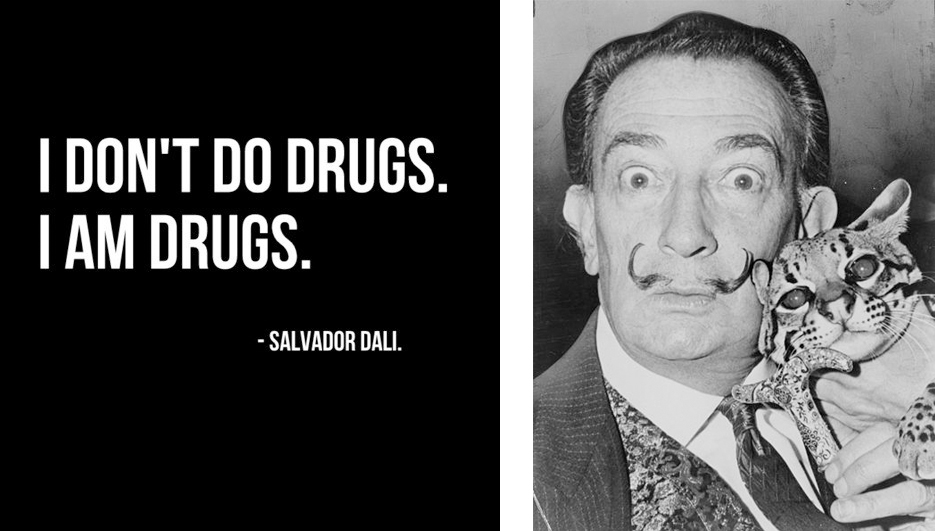
\includegraphics[width=3in]{dali}
\end{frontispiece}
  
%\begin{frontispiece}
%%\begin{flushleft}
%%For in much wisdom is much vexation,\hfill\\
%%\hspace{1.5em}and he who increases knowledge increases sorrow.
%%\end{flushleft}
%%---Eccl.~1:18
%%THIS PAGE INTENTIONALLY LEFT BLANK
%\begin{flushleft}
%\end{frontispiece}

%%%%%%%%%%%%%%%%%%%%%%%%%%%%%

\begin{dedication}
  To my parents, Doug and Carol.
\end{dedication}

%%%%%%%%%%%%%%%%%%%%%%%%%%%%%

\begin{acknowledgments}
  This dissertation would not have been possible without a lifetime of
  edification by others. The foremost of these mentors are my
  parents, who helped my
  interest in science to blossom at an early age \cite{Lew1989}.
  Other strong influences over the years include Kristen Jones, whose
  leadership in high school science bowl stands out particularly;
  Bruce Freeman, who gave invaluable opinions, advice, and support during my
  undergraduate internships; Kevin Clarno, an
  integral force in shaping my interest in reactor analysis and transport
  methods; and the inimitable Todd Urbatsch, whose work and mentoring at LANL
  gave me a solid foundation for my TRT research projects and codes.

  My most recent mentor, Dr. Ed Larsen, has my greatest appreciation and thanks.
  His methodical derivations---as well as his practically limitless patience for
  an upstart like myself---were essential in my graduate education and
  research experiences. The members of my committee also have my grateful
  appreciation for their help in this work.

  In addition to these more formal mentors are my friends over the years who
  have taken something of a mentoring role. Greg Davidson, Jesse Cheatham, and
  Troy Becker transitioned me into graduate school.
  The mentoring and friendship of Shaun and Adrianne Clarke have
  helped me to grow during these years in Michigan. My brother Aaron and sister
  Naomi have remained a source of motivation and endurance.
  Space does not permit me to name the many other friends and family whose
  encouragement
  has been instrumental in helping me struggle through the monumental task of
  writing this thesis.

  I also thank the National Science Foundation for its financial support via
  the Graduate Research Fellowship Program, the Department of Energy for its
  Nuclear Energy University Programs fellowship, and the NERS department for its
  support and its management of the day-to-day necessities.

  Finally, I offer all glory and praise to Jesus Christ, the Creator and my
  Redeemer. Apart from Him, nothing could be possible---especially not this
  dissertation.
\end{acknowledgments}

%%%%%%%%%%%%%%%%%%%%%%%%%%%%%

%\begin{preface}
%  before reading this, you should know\dots
%\end{preface}

% list of contents, etc
\tableofcontents
\listoftables
\listoffigures
%\listofappendices

% % the optional normal abstract is formatted the same as preface and acknowledgements,
% % and is listed in the table of contents
% \begin{abstract}
% \end{abstract}

%%%%%%%%%%%%%%%%%%%%%%%%%%%%%%%%%%%%%%%%%%%%%%%%%%%%%%%%%%%%%%%%%%%%%
% MAIN MATTER
\mainmatter

% note that chapter markers MUST go inside the ``include''-d file
% !TEX root = _individual/introduction.tex

%%%%%%%%%%%%%%%%%%%%%%%%%%%%%%%%%%%%%%%%%%%%%%%%%%%%%%%%%%%%%%%%%%%%%%%%%%%%%%%%
\chapter{Introduction}\label{chap:introduction}
%%%%%%%%%%%%%%%%%%%%%%%%%%%%%%%%%%%%%%%%%%%%%%%%%%%%%%%%%%%%%%%%%%%%%%%%%%%%%%%%

Nuclear engineering is the field in which tools are developed to harness the
power of the
atomic nucleus and high-energy radiation. This field encompasses such
disparate areas as plasma physics, radiation detection, nuclear reactor design,
and atomic particle transport. The latter area is the study of how
statistically large numbers of fundamental particles interact with (and are
``transported'' through) matter: it
accounts for the behavior of neutrons in a nuclear reactor,
gamma rays in shielding applications, electrons in cancer therapy, and photons
in radiative transfer problems. This thesis is concerned with a
particular regime of radiative transfer known as thermal radiative transfer
(TRT).

The difficulty, expense, and impracticality of performing physical
experiments in many fields has produced a tremendous drive to cheaply
simulate physics. The exponentially increasing power and decreasing cost of
computers have led to the rise of computational methods development:
researching and implementing accurate, practical approximations to the physical
equations that describe reality. Our work is in the field of computational
particle transport, and our goal is to develop a new, accurate, inexpensive
approximation to the equations of thermal radiative transfer.

A recent advance in computational methods development is the anisotropic
diffusion (AD)
approximation, recently used to model steady-state neutron transport for
nuclear reactor analysis, viz.~a very high temperature reactor
(VHTR) mock-up \cite{Lar2009c,Tra2011}, for which AD showed promising
results. A similar tensor diffusion
method was also independently formulated for steady-state photon transport
\cite{Mor2007}, but it has not been numerically tested.
Both derivations assumed an infinite medium operating at steady state.
Those two assumptions rarely hold for TRT problems, which typically change
rapidly as a
function of time and necessarily operate in a finite volume. In the new
work presented here, we derive a complete theory describing the anisotropic
diffusion approximation for time-dependent transport problems in finite media.
The new derivation framework allows the development of other ``anisotropic''
approximations. One new member of this family is the anisotropic
\Pone\ method, which is also derived.

Although we develop the theory for a general three-dimensional (3-D) space,
true \mbox{3-D} simulations are expensive because of the expansive problem phase
space: the transport equations operate in three spatial coordinates $(x,y,z)$,
two angular coordinates $(\mu,\theta)$, and time $t$. Even two-dimensional (2-D)
problems, which model a system invariant in the $z$ direction, operate in the
space $(x,y,\mu,\theta,t)$. A ``toy'' geometry called \emph{flatland}
\cite{Abb1884}, recently used in particle transport methods development
\cite{Asa2008,Lar2009c},
reduces the phase space to $(x,y,\theta,t)$ by constraining particles to a
two-dimensional plane. Flatland retains the complexity of multi-dimensional
space while decreasing the computational burden. A notable part of this thesis
is the investigation and application of flatland to transport methods
development.

To verify the accuracy of the newly developed anisotropic theory, it is
necessary to
compare its performance and accuracy against that of existing, proven methods.
Therefore, we compare the AD method against its competitors in several numerical
experiments, most of them using flatland geometry. Due to the complexity of
the thermal radiative transfer process, we first test individual aspects of the
theory. In particular, we verify the predicted boundary conditions in several
steady-state flatland problems \cite{Joh2011a}, and we test the time-dependent
behavior in ``linear'' radiation transport problems, which omit the nonlinear
material--radiation coupling of TRT.

Finally, we apply the new AD approximations to thermal radiative transfer
problems. We begin with
one-dimensional problems in the literature \cite{Rau2005}, and variations
thereof. The primary test bed, though, is a flatland simulation
\cite{Joh2011} inspired by a particular TRT experiment---%
the behavior of a laser-driven shock wave in a small tube filled with xenon
gas---%
in the Center for Radiative Shock Hydrodynamics (CRASH) program
\cite{Crash2010}. In addition to this problem, we test some other difficult
two-dimensional problems \cite{Mou2006}. These comparisons provide a wide and
fair assessment of the AD method, demonstrating both its limitations and its
benefits.

%This thesis extends a steady-state, infinite-medium anisotropic diffusion (AD)
%approximation \cite{Mor2007,Lar2009c} using a systematic derivation from the
%transport equation that accounts for time-dependent behavior and arbitrary
%problem boundaries. Our motivation is to formulate and test an approximation to
%thermal radiative transfer (TRT) that is more accurate than diffusion yet much
%less expensive than a time-dependent transport calculation.

%%%%%%%%%%%%%%%%%%%%%%%%%%%%%%%%%%%%%%%%%%%%%%%%%%%%%%%%%%%%%%%%%%%%%%%%%%%%%%%%
\section{Thermal radiative transfer}

As stated earlier, thermal radiative transfer models the behavior of
energy-transferring photons in hot materials. Radiation is the primary means of
heat transfer in a number of relevant physical problems, such as stellar
astrophysics and fusion experiments \cite{Pom1973,Mih1984}. These systems
operate at the extreme
temperatures necessary to apply the TRT model used in this thesis.

Engineering students know from their heat transfer classes that conduction and
convection transfer energy proportionally to the material
temperature $T$, but radiative energy transfer via black-body emission is
proportional to $T^4$. Thus, when $T$ is very large, conduction and convection
can be neglected, but emission cannot. Other reasonable assumptions
reduce the phenomena of
TRT to the coupling of two dependent variables: the space- and time-dependent material
temperature $T$, and the radiation intensity $I$.

The intensity $I$, analogous to the ``angular flux'' in the reactor physics
world,
describes the state and distribution of photons in space $\vec{x}$, angle
$\vec{\Omega}$, and time $t$.
(In this discussion, we ignore the frequency-dependent nature of radiation.)
The spatial and temporal variables are self-explanatory; the angular
variable essentially determines a photon's velocity${}=c\vec{\Omega}$, using
the speed of light $c$. More photons headed in a certain direction at a certain
point in space-time give rise to a larger value in the intensity---%
an example (outside of TRT) could be an ``intense'' flashlight being shone in
one's eyes.  The time-dependent behavior of the intensity is described by the
Boltzmann transport equation \cite{Dud1976}, sometimes referred to in the
astrophysics literature as the transfer equation \cite{Mih1984}.
The transport equation will be discussed in further detail later.

The second quantity, the material temperature $T(\vec{x},t)$, is a measure of
the amount
of energy stored in the atoms and electrons in the problem at point
$\vec{x}$ at time $t$. When an electron
absorbs a photon, the material energy increases by exactly the amount that the
radiation intensity lost by the absorption event. When the material emits a
photon via the black body process, the lost material energy is transferred to
the radiation field.

The absorption of photons by the material, the black body emission process, and
the straight-line travel of ``streaming'' photons constitute the
thermal radiative transfer process. The rate of absorption of photons is
proportional to the opacity $\sigma$, analogous to the neutron cross section in
reactor physics. Unlike the neutron cross section, the value of $\sigma$ is
a strong function of the material temperature, usually proportional to
$T^{-3}$, so colder materials tend to be more opaque, or optically thick.

Because of the inverse cubic proportionality of the opacity and the quartic
proportionality of radiative emission, most TRT problems share a qualitative
behavior.  The evolution of a system through time tends to show the problem
equilibrating by the progressive deposition of energy within a few mean free
paths of a hot region.  In other words, a layer of cold material will absorb
a great quantity of radiation, heating up and beginning to emit radiation
into the adjacent cold material. This time-dependent evolution is often called
a radiation shock or Marshak wave \cite{Mar1958}.

In summary, the thermal radiative transfer equations describe a physically
complex phenomenon.  The transport equation alone is difficult to model, but
the strong nonlinearity in $\sigma$ and in $T^4$ black body emission make the
TRT equations particularly formidable.
Analytically solving the TRT equations even in the simplest realistic problem
is essentially impossible, hence the need for numerical solutions.
The anisotropic diffusion approximation provides a new method for numerically
solving the radiation transport aspect of the TRT equations.

%%%%%%%%%%%%%%%%%%%%%%%%%%%%%%%%%%%%%%%%%%%%%%%%%%%%%%%%%%%%%%%%%%%%%%%%%%%%%%%%
\section{Overview of TRT solution methods}

The TRT equations have
a large solution phase space and are strongly nonlinear; thus,
they are difficult to solve accurately and quickly. Since the first
simulations of radiative transfer at the dawn of the computer age
\cite{Cam1964,Cam1969}, numerous computational solution methods have been
formulated.  The more useful of these have been reviewed in previous
works \cite{Cam1964,Cam1969,Ols2000,Bru2002,Cas2004,Wol2008};
to give a proper context for the new AD method, we give a brief overview of
them here.

\subsection{Monte Carlo methods}

Generally speaking, the Monte Carlo (MC) method models a random
physical process by simulating the random ``history'' of a statistically large
number
of particles \cite{Bro2004a}. Each stochastic aspect of particle transport---%
birth, collision, scattering, etc.---%
is described by a set of probability distribution functions. Between
events, the simulated particle travels along its stored direction
$\vec{\Omega}$ from its stored position $\vec{x}$. The average behavior of
large numbers of particles (and how large is ``large'' depends on the
complexity of the problem) gives the solution. Each particle history can be
expensive, and the accuracy of the solution is roughly inversely proportional
to the
square root of the number of simulated particles: the Monte Carlo process
gives accurate answers, but it is computationally expensive. 

For linear source-driven transport, which is used e.g.~in reactor analysis, the
solution
methodology is largely intuitive, because each particle is
completely independent from every other. However, the nonlinear nature of the
TRT equations---%
specifically that the behavior of the photons influence the state of the
material, which in turn influences the behavior of other photons---%
makes a Monte Carlo interpretation of TRT far from clear.

The first successful Monte Carlo method for simulating radiative
transfer was Fleck and Cummings' Implicit Monte Carlo (IMC) method
\cite{Fle1971,Wol2008}, which is still widely used today \cite{Urb2006}.
Through the
mathematical process of linearization, it approximates the nonlinear terms in
the TRT equations with linear terms over a short period of time. The
linearization essentially models the process of absorption and
black body re\"emission%
\footnote{For a full discussion of the di\ae resis, refer to R.~McClarren's seminal
work on the inclusion of pretentious footnotes in a dissertation
\cite[p.18]{McC2007}.}%
of photons as isotropic ``pseudo-scattering.'' The resulting linear
transport equation in each time step is solved with Monte Carlo to calculate the
end-of-time-step radiation intensity.

Unlike linear MC methods, IMC does not limit to the exact solution with
increasing number of particles. In addition to the statistical error incurred
by the finite particle count, the linearization of the physics requires
the imposition of both a temporal and a spatial grid, which leads to
truncation errors in time and space. A further complication 
arises because the space and time grids must be properly correlated: for
example, a fine spatial grid with a large time step will produce the unphysical
artifact known as a violation of the maximum principle \cite{Lar1987}.
Additionally, to limit the statistical error (which typically shows up as
random ``noise'' in the solution), the number of particles per
space-time region must remain roughly constant. Finally, unlike linear Monte
Carlo methods, which only need to tally aspects of each particle, IMC requires
that the full state of the radiation intensity be stored in computer memory.
Therefore, generating an accurate fine-mesh solution with IMC can take an
exceedingly large
amount of computer time and memory.

Other Monte Carlo methods \cite{Bro1989,NKa1991,Cha2007a,
Den2004}
have been developed to simulate TRT, but they will not be discussed here.

Even though the IMC method is approximate, it is generally accepted to give
accurate answers, and is thus used as the primary benchmark tool in
our numerical experiments. 

\subsection{Deterministic transport}
Rather than using a ``stochastic'' Monte Carlo interpretation of the physical
process of radiation transport, ``deterministic'' transport methods
approximate the partial differential equation
itself. Deterministic methods make mathematical approximations to the transport
equation, replacing the continuous nature of the variables with discrete
unknowns that can be represented on a computer. The result is a large system of
linear equations that can be solved, typically in an iterative process.

The most popular deterministic method is the discrete ordinates (\SN)
transport method \cite{Lar2010}, which approximates the angular variable
$\vec{\Omega}$ as a quadrature set of discrete directions. There are numerous
ways to discretize the time and space variables, each of which adds the penalty
of discretization error to the solution. In fact, the more subtle effects of
spatial discretization errors were not understood until the late '90s
\cite{Ada1998,Ada2001}.

To use \SN\ for thermal radiative transfer problems, a linearization process
similar to IMC's is performed; it too leads to a pseudo-scattering term.
For purely absorbing steady-state problems, calculating an \SN\ solution is
relatively inexpensive. (We shall take advantage of this property in our
anisotropic diffusion approximation.) However, because of the pseudoscattering
term, \SN\ solutions for TRT problems can converge very slowly.

Like IMC, the \SN\ method requires the full solution of the radiation intensity
$I$ to be stored at the end of each time step. As a transport method, this is
computationally intensive and requires large amounts of storage. These
requirements make high-fidelity transport solutions to some realistic problems
beyond the capability of even today's computers.

\subsection{The diffusion approximation}
If true transport methods are out of reach, it becomes necessary to make
coarser approximations to the transport equation.
%The spherical harmonics (\PN)
%expansion \cite{McC2008a} is the basis for the most popular of these.
%It
%is a different way to approximate the angular dependence of the radiation
%intensity.
The most common course of action is to entirely eliminate the angular variable
from the transport equation, greatly reducing both the computational difficulty
and required storage.

The diffusion approximation has been a mainstay of reactor analysis and TRT
alike since the days of the Manhattan project. In systems whose intensity (or
neutron flux
in the case of nuclear reactors) change very slowly as a function of space, time, and
angle, it is possible to show \cite{Lar1975,Lar1983a} that the transport
solution satisfies a relationship known as Fick's law. This ``law'' states that
the flow of particles is only a function of the gradient of their density:
particles diffuse from areas of high concentration to low concentration.

Diffusion is often used far outside its theoretical range of applicability and
can lead to physically inaccurate answers. A particular artifact of the
diffusion approximation is that, in time-dependent transport, energy can
move faster than the speed of light. One effective but \emph{ad hoc} means to
counter this nonphysical effect is to use a ``flux limiter.''
Flux-limited diffusion (FLD) can provide qualitatively accurate answers to
certain TRT problems \cite{Ols2000}, and computationally it is relatively
inexpensive, so it a common means of simulating TRT.

%%%%%%%%%%%%%%%%%%%%%%%%%%%%%%%%%%%%%%%%%%%%%%%%%%%%%%%%%%%%%%%%%%%%%%%%%%%%%%%%
\section{Contribution of this work}

The different approximations to TRT are represented qualitatively in
Fig.~\ref{fig:fidelity}.

\begin{figure}[htb]
  \centering
  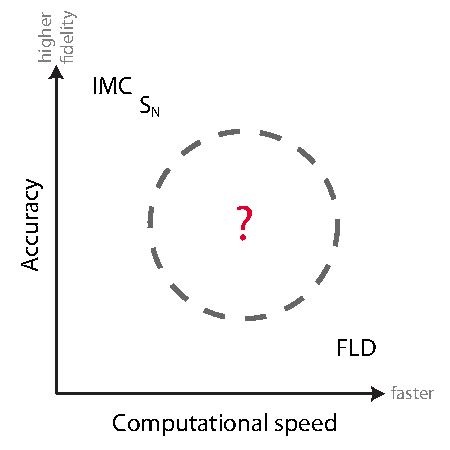
\includegraphics[width=3in]{fidelity}
  \caption{Figurative representation of existing TRT methods, showing the
  trade-off between accuracy and speed.}
  \label{fig:fidelity}
\end{figure}

With our development of anisotropic diffusion and its application to TRT, we
hope to provide a new solution process that is much less expensive than
full-fledged transport but more theoretically robust than standard diffusion or
FLD. Such a method would fit near the question mark in
Fig.~\ref{fig:fidelity}.

%%%%%%%%%%%%%%%%%%%%%%%%%%%%%%%%%%%%%%%%%%%%%%%%%%%%%%%%%%%%%%%%%%%%%%%%%%%%%%%%
\section{Synopsis}

The remainder of this thesis is organized into the following chapters.

\chaptersynopsis{chap:trtBackground}
The assertions about the difficulty of computational modeling of thermal
radiative transfer are bolstered by presenting the equations themselves. We give
a brief overview of existing approximations to the TRT equations and discuss how
those approximations are used in our work. Particular emphasis is given to the
semi-implicit treatment, which allows the nonlinear problem to be approximated
by a system of linear equations.

\chaptersynopsis{chap:adDerivation}
With the transport equation in hand, we derive a new approximation to radiation
transport, anisotropic diffusion. The derivation accounts for both time
dependence and boundary conditions. We then discuss some of the properties of
the AD method and make predictions for its range of applicability.

\chaptersynopsis{chap:aponeDerivation}
The derivation of the time-dependent AD equations assumed that the solution
changes slowly in time, which can be a poor approximation when applied to
TRT: it can actually lead to the nonphysical transfer of energy faster than the
speed of
light. This chapter addresses that shortcoming by modifying the ansatz used in
deriving the anisotropic diffusion equations, leading to a new ``anisotropic
\Pone'' method.

\chaptersynopsis{chap:implementation}
The leakage terms for anisotropic diffusion are more complex than standard
diffusion: rather than a scalar diffusion coefficient, AD has a diffusion
tensor. This necessitates unusual discretization schemes in all but the simplest
of problems. We present new discretization schemes for Cartesian \xy\ geometry
that can account for the transverse leakage induced by the anisotropic diffusion
tensor.

\chaptersynopsis{chap:flatland}
As mentioned earlier, the ``flatland'' geometry has recently proven to be a
valuable test bed for new transport methods because of its smaller phase space
and correspondingly easier solution. This chapter gives a thorough overview of
the differences between flatland and true 3-D geometries, with a focus on
implementing flatland solvers. We also explore diffusion in flatland, not only
deriving the prior result that the diffusion coefficient is different but also
formulating correct diffusion boundary conditions. Finally, we present the AD
equations in flatland geometry.

\chaptersynopsis{chap:simpleNumericalResults}
Before applying the anisotropic approximations to full nonlinear transport in
multi-dimensional geometries, it is important that we test individual components
of the derivation. We detail several steady-state problems that test the
discretization schemes, flatland diffusion boundary conditions, and anisotropic
diffusion boundary conditions. We also test some simple linear transport
problems.

\chaptersynopsis{chap:trtNumericalResults}
Finally, we test the applicability of the anisotropic methods to the nonlinear
TRT equations. To begin, we examine a few simple 1-D test problems, where the
anisotropic methods merely ``smear'' the diffusion coefficients spatially.
This provides a test bed for determining the robustness of the nonlinear
treatment. Then
we move to more complicated flatland problems that simulate radiation flow
through an optically thin channel. (This is the qualitative configuration of
the CRASH problem.)
Additionally, we apply the AD method to some difficult 2-D problems in the
literature that feature optically thick obstacles rather than optically thin
streaming channels.

\chaptersynopsis{chap:conclusion}
The final chapter summarizes the results of the theory developed in this thesis
and its application to TRT problems. We discuss possible improvements to the new
methods and other future work.


% !TEX root = _individual/trtBackground.tex

%%%%%%%%%%%%%%%%%%%%%%%%%%%%%%%%%%%%%%%%%%%%%%%%%%%%%%%%%%%%%%%%%%%%%%%%%%%%%%%%
\chapter{Background to Thermal Radiative Transfer}\label{chap:trtBackground}

Thermal radiative transfer (TRT) is the nonlinear process describing the
dominant form of energy transfer in a very hot material, such as the interior
of a star or the
target of a laser fusion experiment. The equations that model TRT are
time-dependent, contain strong nonlinearities, and reside in a large phase
space. These difficulties make TRT the subject of significant work in methods
development.

A full representation of the physics in
those high-energy-density regimes often includes the consideration of moving
relativistic materials, different electron and ion temperatures, photon
scattering, and thermal conduction in the material \cite{Mih1984}. However,
much theoretical work in the field neglects these complex phenomena by
\begin{itemize}
  \item working in a fixed medium, disregarding material advection;
  \item assuming local thermodynamic equilibrium (LTE), which uses a single
    material temperature;
  \item neglecting photon scattering, which tends to be comparatively small for
    very hot materials; and
  \item neglecting thermal conduction, since energy transfer is dominated by
    radiative transfer in the temperature regimes we consider.
\end{itemize}

A further simplification often used for methods development is the ``gray''
approximation to the frequency dependence. Analogous to the one-group
approximation for neutron transport, the full transport equation is integrated
over all frequencies, and the opacities are averaged with some \emph{a priori}
weighting function. The commonly used Rosseland mean satisfies a radiation
diffusion equation found in an asymptotic analysis of the thermal radiative
transfer equations \cite{Lar1983a} and is therefore the best choice for a
method that resembles diffusion.

%%%%%%%%%%%%%%%%%%%%%%%%%%%%%%%%%%%%%%%%%%%%%%%%%%%%%%%%%%%%%%%%%%%%%%%%%%%%%%%%
\section{TRT equations}\label{sec:trtEquations}
After the simplifications, the thermal radiative transfer process can be
described by
\begin{subequations} \label{eqs:fullGrayTRT}
the radiative transfer equation,
\begin{equation} \label{eq:fullGrayTransport}
  \frac{1}{c} \pder{I}{t}
  + \vec{\Omega} \vd \del I +
 \sigma I
  = \frac{\sigma c U_r}{4\pi} 
  + \frac{c Q}{4\pi} \,,
\end{equation}
and the material energy balance equation
\begin{equation} \label{eq:fullGrayMaterial}
  \pder{U_m}{t} = \sigma \int_{4\pi}  I \ud \Omega - \sigma c U_r
  %= \sigma \phi - \sigma c U_r
  \,.
\end{equation}
\end{subequations}

The notation and omitted parameters in Eqs.~\eqref{eqs:fullGrayTRT} are:
\begin{alignat*}{2}
  I &= I(\vec{x}, \vec{\Omega}, t) &&= \text{the angle-dependent
  radiation intensity,}
%  \\
%  \phi &= \phi(\vec{x}, t) &&= \text{the zeroth angular moment of the radiation
%  intensity,}
  \\
  T &= T(\vec{x}, t) &&= \text{the temperature of the material,}
  \\
  \sigma &= \sigma(\vec{x}, T) &&= \text{the absorption opacity,} 
  \\
  Q &= Q(\vec{x}) &&= \text{an extraneous isotropic radiation energy source,}
  \\
  U_m &= U_m(\vec{x}, T) &&= \text{the material energy density,}
  \\
  U_r &= U_r(\vec{x}, T) &&= \text{the equilibrium radiation energy density of
  the material,}
  \\
  c_v &= c_v(\vec{x}, T) &&= \text{the specific heat capacity of a material,}
  \\
  c& &&= \text{the speed of light.}
\end{alignat*}
The ``equilibrium radiation energy density'' of a material is a scaled integral
of the Planckian emission function:
\begin{subequations} \label{eqs:materialU}
\begin{equation} \label{eq:radEnergyDens}
  U_r(T) \equiv aT^4 = \frac{1}{c} \int_{4\pi} \int_{0}^{\infty}B(\nu, T) \ud
  \nu \ud \Omega \,.
\end{equation}
The material energy density is related only to the material's temperature:
\begin{equation} \label{eq:matEnergyDens}
  U_m(T) = \int_{0}^{T} c_v(T') \ud T' \,.
\end{equation}
The specific heat capacity $c_v(T)$ is the amount of energy per unit
volume needed to change the material's temperature.
\end{subequations}
%The zeroth moment of $I$ is equal to the radiation energy density scaled by the
%speed of light:
%\begin{equation*}
%  \phi(\vec{x}, t) = \int_{4\pi} I(\vec{x}, \vec{\Omega}, t) \ud \Omega
%  = \int_{4\pi} c [h \nu] N(\vec{x}, \vec{\Omega}, t) \ud \Omega
%  = c \RadEn(\vec{x}, t)\,.
%\end{equation*}
%Here, $N$ is the photon density, $h\nu$ is the energy of a single photon, and
%$E$ is the radiation energy density.

The scalar
intensity is the energy density of the radiation scaled by the speed of light:
$\phi=cE$, so integrating $\phi$ over a volume at time $t$ and dividing by $c$
gives the amount of energy in the radiation field in that volume.
%%%%%%%%%%%%%%%%%%%%%%%%%%%%%%%%%%%%%%%%%%%%%%%%%%%%%%%%%%%%%%%%%%%%%%%%%%%%%%%%
\section{Radiation transport approximations}\label{sec:trtApproxMethods}

The large phase space and nonlinearity of Eqs.~\eqref{eqs:fullGrayTRT} makes a
direct solution intractable except for the simplest of problems
\cite{Su1997,Mos2006}. A more complete overview of the approximations is given
in \cite{Bru2002,Ols2000,Wol2008}.

All of the approximations trade speed for accuracy. The fewer unknowns a method
has, the easier it is to solve.

%%%%%%%%%%%%%%%%%%%%%%%%%%%%%%%%%%%%%%%%
\subsection{Implicit Monte Carlo}

%%%%%%%%%%%%%%%%%%%%%%%%%%%%%%%%%%%%%%%%
\subsection{Discrete ordinates}

%%%%%%%%%%%%%%%%%%%%%%%%%%%%%%%%%%%%%%%%
\subsection{Spherical harmonics}
\cite{McC2008a}

%%%%%%%%%%%%%%%%%%%%%%%%%%%%%%%%%%%%%%%%
\subsection{Diffusion}\label{sec:diffusion}

%%%%%%%%%%%%%%%%%%%%%%%%%%%%%%%%%%%%%%%%
\subsection{Flux-limited diffusion}\label{sec:fldBackground}

The radiation intensity satisfies the mathematical identity $\norm{F} \le \phi$,
essentially limiting the leakage of radiation at a point to the radiation
energy at that point. The identity can be proven using the triangle inequality:
\begin{align*}
  \norm{\vec{F}} &= \norm{ \int_{4\pi} \vec{\Omega} I \ud \Omega}
  \\&\le \int_{4\pi} \norm{\vec{\Omega}} \abs{I} \ud \Omega 
  \\
  &\le \int_{4\pi} [1] I \ud\Omega
  \\
  \norm{\vec{F}} &\le \phi\,.
\end{align*}

\subsubsection{Flux limiters}

\subsubsection{Flux limiter discretization}
\cite{Ols2007}

%%%%%%%%%%%%%%%%%%%%%%%%%%%%%%%%%%%%%%%%%%%%%%%%%%%%%%%%%%%%%%%%%%%%%%%%%%%%%%%%
\section{Semi-implicit linearization}

To solve the TRT equations with deterministic methods,\footnote{The Implicit
Monte Carlo scheme of Fleck and Cummings \cite{Fle1971} gives a result very
similar to the semi-implicit discretization. The difference is that Monte
Carlo does not need to approximate the time dependence implicitly.} we use the
semi-implicit time
discretization scheme \cite{Kno1999a,Kno2001,Low2004} where some important
unknowns are treated implicitly in
time, and other unknowns are treated explicitly. By choosing the intensity $I$
and equilibrium radiation energy density $U_r$ to be the implicit variables and 
by treating the opacity $\sigma$ and another material property explicitly,
Eqs.~\eqref{eqs:fullGrayTRT} can be formulated as a time-dependent linear
transport equation over a time step $t^n < t < t^{n+1}$.

\subsection{Linearizing the material energy equation}
First, we define a parameter $\beta$ as a function of Eqs.~\eqref{eqs:materialU}:
\begin{equation} \label{eq:beta}
  \beta(T) = \pder{U_r}{U_m} 
  = \pder{U_r}{T} \Bigg/ \pder{U_m}{T}
  = \frac{4 a T^3}{c_v(T)} \,.
\end{equation}
The chain rule allows the left hand side of Eq.~\eqref{eq:fullGrayMaterial} to be
expressed without approximation in terms of the equilibrium radiation energy
density $U_r$:
\begin{equation*}
  \pder{U_m}{t} = \pder{U_m}{U_r} \pder{U_r}{t} = \frac{1}{\beta(T)}
  \pder{U_r}{t} = \sigma \int_{4\pi}  I \ud \Omega - \sigma c U_r \,.
\end{equation*}
The first approximation is to ``freeze'' the parameter $\beta$ at the beginning-of-time-step temperature $T^n$:
\begin{equation}\label{eq:frozenBeta}
  \frac{1}{\beta^n}
  \pder{U_r}{t} \approx \sigma \int_{4\pi}  I \ud \Omega - \sigma c U_r \,.
\end{equation}
The process of freezing $\beta$ is equivalent to approximating the
Planckian emission term with a Taylor series \cite{Kno2007}.

Because the approximation to $\beta$ is an approximation to the rate of change
in material energy, this equation no longer conserves the system's total
energy. To enforce conservation of energy over a time step, we must set the
material energy change over a time step to the time-integrated approximation:
\begin{align}
  \nonumber
  \int_{t^n}^{t^{n+1}}  \pder{U_m}{t}\ud t &= \frac{1}{\beta^n}
  \int_{t^n}^{t^{n+1}} \pder{U_r}{t}\ud t
  \\
  \nonumber
  U_m^{n+1} - U_m^n &= \frac{1}{\beta^n} \left[ U_r^{n+1} - U_r^n \right]
  \\
  \label{eq:matenConservationUpdate}
  U_m^{n+1} &=  U_m^n + \frac{U_r^{n+1} - U_r^n}{\beta^n}\,.
\end{align}
%Thus, the expression of $\tpder{U_m}{t}$ in terms of $\tpder{U_r}{t}$

The next approximation is to explicitly freeze the opacity $\sigma$ in
Eq.~\eqref{eq:frozenBeta}:
\begin{equation*}
  \frac{1}{\beta^n}
  \pder{U_r}{t} \approx \sigma^n \int_{4\pi}  I \ud \Omega - \sigma^n c U_r \,.
\end{equation*}
Now we can time-average the material equation to express it in terms of two
simple time-average unknowns. Operating by
$\frac{1}{\Delta_t^n}\int_{t_n}^{t^{n+1}} (\cdot) \ud t$,
\begin{equation*}
  \frac{1}{\beta^n}
  \frac{U_r^{n+1} - U_r^n}{\Delta_t^n} = \sigma^n \int_{4\pi} \left[
  \frac{1}{\Delta_t^n}\int_{t_n}^{t^{n+1}} I\ud t
  \right] \ud \Omega - \sigma^n c \left[
  \frac{1}{\Delta_t^n}\int_{t_n}^{t^{n+1}} U_r \ud t \right]\,.
\end{equation*}
Next, we apply the implicit Euler approximation to $U_r(\vec{x}, \vec{\Omega},
t)$ and $I(\vec{x}, \vec{\Omega}, t)$ by setting their time-averaged values to
the values at $t^{n+1}$:
\begin{equation} \label{eq:semiImplicitMaterial}
  \frac{1}{\beta^n(\vec{x})}
  \frac{U_r^{n+1}(\vec{x}) - U_r^n(\vec{x})}{\Delta_t^n}
  = \sigma^n(\vec{x}) \int_{4\pi} I^{n+1}(\vec{x}, \vec{\Omega})\ud \Omega
  - c \sigma^n(\vec{x}) U_r^{n+1}(\vec{x}) \,.
\end{equation}

We solve Eq.~\eqref{eq:semiImplicitMaterial} for $U_r^{n+1}$ in order to
eliminate the implicit dependence of the transport equation on the material
energy equation.
\begin{align} \nonumber
  U_r^{n+1} - U_r^n
  &= \beta^n \Delta_t^n \sigma^n\int_{4\pi} I^{n+1}\ud \Omega
   - c \beta^n \Delta_t^n \sigma^n U_r^{n+1}
   \\ \nonumber
  U_r^{n+1} [ 1 + c \beta^n \Delta_t^n \sigma^n ]
  &= \beta^n \Delta_t^n \sigma^n\int_{4\pi} I^{n+1}\ud \Omega + U_r^n
   \\ \nonumber
  U_r^{n+1}
  &= \frac1c \frac{ c \beta^n \Delta_t^n \sigma^n }{ 1 + c \beta^n \Delta_t^n \sigma^n}
  \int_{4\pi} I^{n+1}\ud \Omega + \frac1{ 1 + c \beta^n \Delta_t^n \sigma^n}
  U_r^n
  \\ \nonumber
  U_r^{n+1}
  &= \left[1 - \frac{1 }{ 1 + c \beta^n \Delta_t^n \sigma^n} \right]
  \int_{4\pi} I^{n+1}\ud \Omega + \frac1{ 1 + c \beta^n \Delta_t^n \sigma^n}
  U_r^n
  \\ \label{eq:urNPlusOne}
  U_r^{n+1}
  &= \left(1 - f^n\right) \frac1c \int_{4\pi} I^{n+1}\ud \Omega + f^n U_r^n
\end{align}
where
\begin{equation} \label{eq:fleckFactor}
  f^n = f^n(\vec{x}) \equiv \left[ 1 + \beta^n c \Delta_t^n \sigma^n
  \right]\inv \,.
\end{equation}
This semi-implicit formulation is very similar to the linearization in Fleck
and Cummings' IMC method \cite{Fle1971}, although they leave the intensity $I$
in a time-dependent form.

\subsection{Linearizing the transport equation}
The next step is apply similar approximations to the nonlinear radiation
transport equation~\eqref{eq:fullGrayTransport}. As with the material equation,
the
opacities are ``frozen'' at their beginning-of-time-step values $\sigma^n$, and
the equation is time-averaged:
\begin{multline*}
  \frac{1}{c} \frac{I^{n+1} - I^n}{\Delta_t^n}
  + \vec{\Omega} \vd \del \left[
  \frac{1}{\Delta_t^n}\int_{t_n}^{t^{n+1}} I\ud t
  \right] +
 \sigma^n \left[
  \frac{1}{\Delta_t^n}\int_{t_n}^{t^{n+1}} I\ud t
  \right]
  \\
  = \frac{\sigma^n c}{4\pi} \left[
  \frac{1}{\Delta_t^n}\int_{t_n}^{t^{n+1}} U_r \ud t \right]
  + \frac{1}{4\pi}\left[
  \frac{1}{\Delta_t^n}\int_{t_n}^{t^{n+1}} Q \ud t \right] \,.
\end{multline*}
Since the extraneous energy source $Q$ is assumed to be known \emph{a priori},
we let its time-averaged value be $Q^n$. As in the material equation, we apply
the implicit Euler approximation to $I$ and $U_r$:
\begin{equation*}
  \frac{1}{c} \frac{I^{n+1} - I^n}{\Delta_t^n}
  + \vec{\Omega} \vd \del I^{n+1}
 + \sigma^n I^{n+1}
 = \frac{\sigma^n c}{4\pi} U_r^{n+1}
  + \frac{c}{4\pi} Q^n \,.
\end{equation*}
Finally, we substitute $U_r^{n+1}$ from Eq.~\eqref{eq:urNPlusOne},
which was derived from the material equation Eq.~\eqref{eq:fullGrayMaterial}:
\begin{align}\nonumber
  \frac{1}{c} \frac{I^{n+1} - I^n}{\Delta_t^n}
  + \vec{\Omega} \vd \del I^{n+1}
 + \sigma^n I^{n+1}
 &= \frac{\sigma^n c}{4\pi} \left[ \left(1 - f^n\right) \frac1c \int_{4\pi} I^{n+1}\ud \Omega + f^n U_r^n \right]
  + \frac{c}{4\pi} Q^n
  \\ \label{eq:linearizedGrayTransport}
  \frac{1}{c} \frac{I^{n+1} - I^n}{\Delta_t^n}
  + \vec{\Omega} \vd \del I^{n+1}
 + \sigma^n I^{n+1}
 &=  \left(1 - f^n\right) \sigma^n \frac{1}{4\pi} \int_{4\pi} I^{n+1}\ud \Omega
 + \frac{1}{4\pi} f^n \sigma^n c U_r^n
  + \frac{1}{4\pi} c Q^n \,.
\end{align}

\subsection{Comments}\label{sec:trtLinearizedComments}
If we compare Eq.~\eqref{eq:linearizedGrayTransport} to a temporally implicit
discretization of a monoenergetic linear transport problem with isotropic
scattering,
\begin{equation*}
  \frac{1}{v} \frac{\psi^{n+1} - \psi^n}{\Delta_t^n} 
  + \vec{\Omega} \vd \del \psi^{n+1}
 + \Sigma_t \psi^{n+1}
 = \frac{1}{4\pi} \int_{4\pi} \psi^{n+1}\ud \Omega
  + \frac{1}{4\pi} q \,,
\end{equation*}
we find equivalences between the two:
\begin{alignat*}{2}
  I &\leftrightarrow \psi &&= \text{the angular flux,}
  \\
  \sigma^n &\leftrightarrow \Sigma_t &&= \text{the total cross section,}
  \\
  \left(1 - f^n\right) \sigma^n &\leftrightarrow \Sigma_s &&= \text{the scattering cross
  section,} 
  \\
  f^n \sigma^n c U_r^n + c Q^n &\leftrightarrow q &&= \text{the isotropic source for time
  step $n$,}
  \\
  v   &\leftrightarrow c &&= \text{the particle velocity.}
\end{alignat*}
Even though the original radiation transport equation was purely
absorbing, the linearization scheme created a ``pseudoscattering''
term that essentially emulates the absorption and isotropic reemission of
radiation during a time step. The IMC literature often refers to the
``effective scattering opacity,''
$\sigma_\text{es}^n \equiv \left(1 - f^n\right) \sigma^n$.

Furthermore, if we take the zeroth angular moment of
Eq.~\eqref{eq:linearizedGrayTransport} and let $\phi^{n+1}(\vec{x}) \equiv
\frac{1}{4\pi} \int_{4\pi} I^{n+1}\ud \Omega$, then we find the radiation
energy conservation equation over the time step to be
\begin{equation}\label{eq:semiImplicitZeroth}
  \frac{1}{c} \frac{\phi^{n+1} - \phi^n}{\Delta_t^n}
  + \del \vd \vec{F}^{n+1} + f^n\sigma^n \phi^{n+1}
 =  f^n \sigma^n c U_r^n + c Q^n\,.
\end{equation}
The quantity, $\sigma_\text{ea}^n \equiv f^n\sigma^n$ is known as the
``effective absorption opacity.''

\subsection{Solution process summary}
The time-dependent radiation solution is stored in the linear time-dependent
transport solver. The material energy $U_m$ must be stored, but the
material temperature can be either stored (highly recommended because of its
frequent use) or calculated on the fly from $U_m$ by inverting the integral in
Eq.~\eqref{eq:matEnergyDens}.

For the $n$th time step, given the initial radiation field $I^{n}$ and the
initial material energy density $U_m^n$, the solution process follows.
\begin{enumerate}
  \item Linearize the system. Using the starting temperature $T^n$, calculate
    the frozen $\sigma^n$ and $\beta^n$ in each spatial cell. Use
    Eq.~\eqref{eq:fleckFactor} to calculate $f^n$, which in turn is used to
    calculate the linearized isotropic source $f^n \sigma^n c U_r^n + c Q^n$
    and the effective scattering cross section $\left(1 - f^n\right) \sigma^n$.
    If using a diffusion method to approximate the transport solution, the
    absorption cross sections and diffusion coefficients must be recalculated.
  \item Solve the linear transport problem for $\psi^{n+1}=I^{n+1}$. The new
    radiation
    temperature can optionally be calculated:
    \begin{equation*}
      a (T_\text{rad}^{n+1})^4 = \frac{1}{c} \int_{4\pi} I^{n+1}
      \ud \Omega
%      \lra
%      (T_\text{rad}^{n+1})^4 = \frac{1}{ac} \phi^{n+1}
      \lra
      T_\text{rad}^{n+1}(\vec{x}) = \left[ \frac{\phi^{n+1}(\vec{x})}{ac} \right]^{1/4}\,.
    \end{equation*}
  \item Update the material temperature. From Eq.~\eqref{eq:urNPlusOne}
    we can calculate the linearized estimate of $U_r^{n+1}$:
    \begin{equation*}
      U_r^{n+1} = \left(1 - f^n\right) \frac1c \phi^{n+1}  + f^n U_r^n\,.
    \end{equation*}
    However, because of the linearization of $\beta$, $U_r^{n+1} \ne a
    (T^{n+1})^4$. Instead, to calculate the material temperature, we must use
    Eq.~\eqref{eq:matenConservationUpdate}. Substituting
    Eq.~\eqref{eq:urNPlusOne} into Eq.~\eqref{eq:matenConservationUpdate}
    and simplifying gives
    \begin{equation}\label{eq:matenConservationUpdate2}
      U_m^{n+1} =  U_m^n + f^n \sigma^n \Delta_t^n \left[ \phi^{n+1} - c U_r^n \right] \,.
    \end{equation}
    [This form can also be derived by integrating
    Eq.~\eqref{eq:fullGrayMaterial} over a time step after making the
    approximation $\sigma(T) \approx \sigma(T^n)$.]
\end{enumerate}

Figure~\ref{fig:semiImplicitFlowchart} shows how the quantities $\Delta_t$,
$\beta$, $\sigma$, $f$, etc.~relate. This relation is especially important when
implementing the linearization scheme programmatically. 
\begin{sidewaysfigure}[hp]
  \centering
  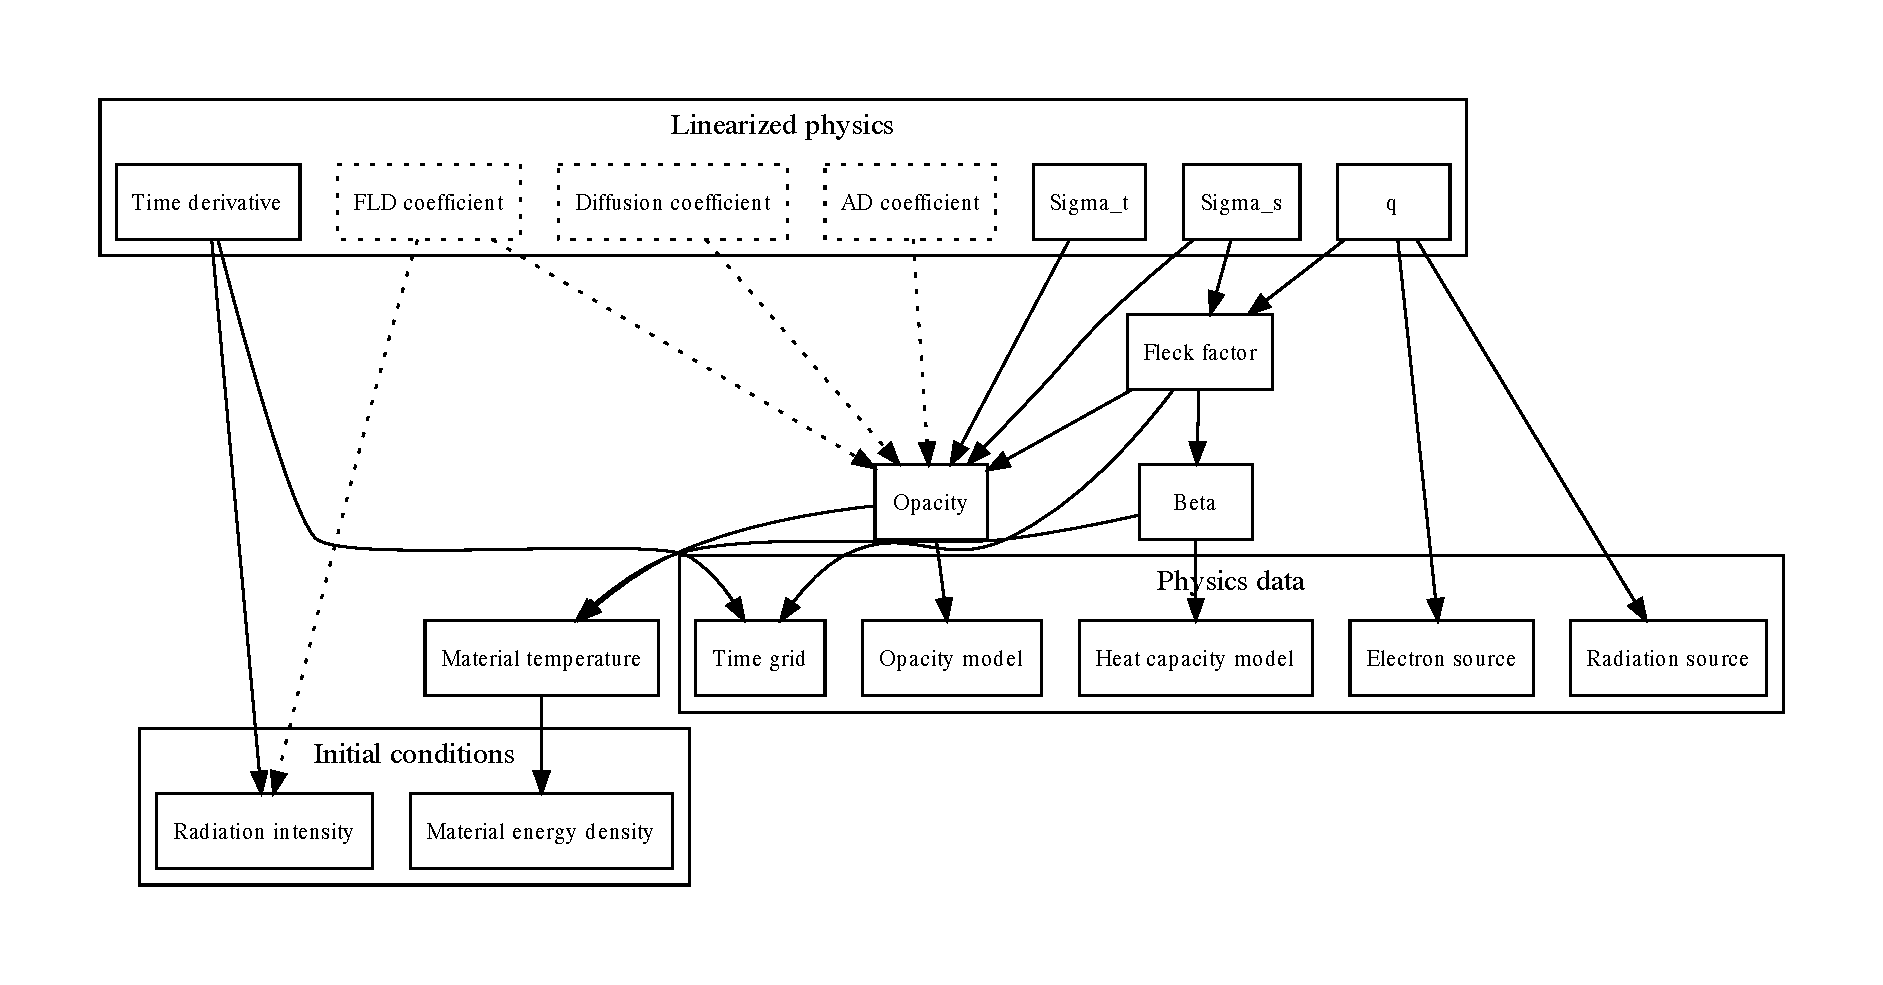
\includegraphics[width=8in]{semi-implicit}
  \caption{Dependency graph of quantities in the semi-implicit discretization.}
  \label{fig:semiImplicitFlowchart}
\end{sidewaysfigure}


% !TEX root = _individual/adDerivation.tex

\newcommand{\epsiloncolor}[1]{#1}
%%%%%%%%%%%%%%%%%%%%%%%%%%%%%%%%%%%%%%%%%%%%%%%%%%%%%%%%%%%%%%%%%%%%%%%%%%%%%%%%
\chapter{Anisotropic diffusion theory}

The previous work in anisotropic diffusion has only considered a steady-state
problem in an infinite medium \cite{Lar2009c,Mor2007}. The new understanding of
the AD method presented in this chapter provides a theoretical basis for
using the AD method in time-dependent and nonlinear contexts, and it also
addresses the heretofore unsolved problem of how to treat the boundary
conditions.

A summary of the derivation is presented up front:
\begin{enumerate}
  \item Consider the time-dependent nonlinear radiation transport equation
    over one time step, with the opacities frozen at some particular value.
  \item Define the anisotropic intensity as $\Psi = I - \frac{1}{4\pi}\phi$.
    From the radiation transport equation and conservation equation, we get a
    transport equation for $\Psi$ with appropriate initial and boundary
    conditions.
  \item Transform this to an integral transport equation for $\Psi$, and move
    the term involving $\phi$ to the right-hand side to get an exact
    integral expression for $I$.
  \item Use Taylor series to approximate nonlocal unknowns with local
    unknowns.
  \item Require that the contribution of boundary terms throughout the problem
    space is zero: this gives boundary conditions for the new approximate
    method.
  \item Take the first angular moment of this new approximate angular
    intensity to get an approximate radiation flux.
  \item Substitute into time-dependent particle conservation equation to get
    time-dependent anisotropic diffusion.
\end{enumerate}

%%%%%%%%%%%%%%%%%%%%%%%%%%%%%%%%%%%%%%%%%%%%%%%%%%%%%%%%%%%%%%%%%%%%%%%%%%%%%%%%
\section{Derivation}
The gray radiative transfer equation inside a time step $0 < t < \Delta_t$,
with opacities frozen at some value $\sigma^\ast$ (which could be
$\sigma(\vec{x},0)$ for a semi-implicit formulation), is:
\begin{subequations} \label{eqs:fullTransport}
\begin{multline} \label{eq:fullTransportVol}
  \frac{1}{c} \pder{I}{t}(\vec{x}, \vec{\Omega}, t)
    + \vec{\Omega}\vd \grad I(\vec{x}, \vec{\Omega}, t)
    + \sigma^\ast(\vec{x}) I (\vec{x}, \vec{\Omega}, t)
    \\ = \frac{1}{4\pi} \sigma^\ast(\vec{x}) ac [T(\vec{x}, t)]^4
    + \frac{1}{4\pi} q_{r}(\vec{x}, t)
    \equiv \frac{1}{4\pi} Q(\vec{x}, t)
    \equiv \hat Q(\vec{x}, \vec{\Omega}, t) \,,
\\
x \in V,\  0 \le t < \Delta_t, \ \vec{\Omega} \in 4\pi,
\end{multline}
with the boundary condition
\begin{equation} \label{eq:fullTransportBndy}
  I(\vec{x}, \vec{\Omega}, t) = I^b(\vec{x}, \vec{\Omega}, t) \,,
 \quad \vec{x} \in \partial V, \ \vec{\Omega} \vd \vec{n} < 0,\ 0 \le t < \Delta_t
\end{equation}
and the initial condition
\begin{equation} \label{eq:fullTransportInit}
 I(\vec{x}, \vec{\Omega}, 0) = I^i(\vec{x}, \vec{\Omega}, t) \,,
 \quad \vec{x} \in V, \ \vec{\Omega} \in 4\pi\,.
\end{equation}
(The initial condition here is usually the solution from the previous time
step.)
\end{subequations}

We can express the left-hand side of Eq.~\eqref{eq:fullTransportVol} as a
transport operator $\lop{\cdot}$ that satisfies
\begin{equation*}
  \lop{I(\vec{x}, \vec{\Omega}, t)} = \hat Q(\vec{x}, \vec{\Omega}, t)
  + \text{boundary conditions} + \text{initial conditions}\,.
\end{equation*}

The particle conservation equation (a scaled form of radiation energy
conservation) is the zeroth moment of the radiation transport equation.
\begin{subequations} \label{eqs:loEquations}
Operating on Eq.~\eqref{eq:fullTransportVol} by $\int_{4\pi} (\cdot) \ud
\Omega$ gives
\begin{equation} \label{eq:loVol}
\frac{1}{c} \pder{\phi}{t} (\vec{x}, t)
  + \grad \vd\vec{F}(\vec{x}, t)
  + \sigma^\ast \phi(\vec{x}, t)
  =  Q(\vec{x}, t)\,.
\end{equation}
Doing the same to the initial condition, Eq.~\eqref{eq:fullTransportInit},
\begin{equation} \label{eq:loInit}
\phi(\vec{x}, 0) = \int_{4\pi}  I^i(\vec{x},
\vec{\Omega}) \ud \Omega = \phi^i(\vec{x}) \,.
\end{equation}
\end{subequations}
Here we have used the scalar intensity $\phi=\int_{4\pi} I \ud \Omega$ and the
radiation flux $\vec{F} = \int_{4\pi} \vec{\Omega} I \ud \Omega$. The boundary
conditions shall be addressed later.

\subsection{Integral transport equation}
Because the opacities are frozen (i.e., independent of time inside $\Delta_t$),
and assuming the arbitrary angle- and space-dependent $\hat Q(\vec{x}, t)$ is
known inside the time step,
the transport operator can be
inverted to yield an integral equation for the time-dependent angular
intensity $I$ \cite{Pri2010}. The exact result for the intensity is:
\begin{subequations} \label{eqs:inverseTransport}
  \begin{align} \label{eq:inverseTransportFull}
  \begin{split}
    I(\vec{x}, \vec{\Omega}, t)
    &=
    I^b(\vec{x}_b, \vec{\Omega}, t - \norm{\vec{x} - \vec{x}_b}/c)
    \eexp^{ -\tau(\vec{x}, \vec{x}_b)}
    U(ct - \norm{\vec{x} - \vec{x}_b})
    \\
    &\qquad + I^i( \vec{x} - ct \vec{\Omega}, \vec{\Omega})
    \eexp^{ -\tau(\vec{x}, \vec{x} - ct \vec{\Omega})}
    U( \norm{\vec{x} - \vec{x}_b} - ct)
    \\
    &\qquad +  \int_{0}^{\norm{\vec{x} - \vec{x}_b}}
    \left[ \hat Q(\vec{x} - s \vec{\Omega}, \vec{\Omega}, t-s/v)
    \right]
    \eexp^{ -\tau(\vec{x}, \vec{x} - s \vec{\Omega})}
    \ud s\,.
  \end{split}
    \\ 
    &\equiv \lopinv{b}{I^b}
    + \lopinv{i}{I^{\smash i \vphantom{\mathrm{i}}}}
    + \lopinv{v}{\hat Q} 
  \end{align}
  Here, $U(\zeta)$ is the heaviside function, unity for $\zeta \ge 0$ and zero
  otherwise. The optical thickness of the medium between points $\vec{x}$ and
  $\vec{x}'$ along direction $\vec{\Omega} = (\vec{x}'-
  \vec{x})/\norm{\vec{x}'-\vec{x}}$ is 
  \begin{equation} \label{eq:fullTauDefinition}
    \tau(\vec{x}, \vec{x}') = \int_{0}^{\norm{\vec{x} -
    \vec{x}'}} \sigma^\ast(\vec{x}-s\vec{\Omega}) \ud s \,.
  \end{equation}
  The point $\vec{x}_b$ is defined as the point on the boundary that,
  following direction $\vec{\Omega}$, intersects point $\vec{x}$. In other
  words, $\vec{x}_b = \vec{x} - s \vec{\Omega}$ where $s$ positive and fixed
  for a particular $(\vec{x}, \vec{\Omega})$.
\end{subequations}

Just as $\lop{\cdot}$ represented a differential operator, $\lopinv{}{\cdot}$
represents an integral operator.
Equation~\eqref{eq:lopinv} shows how the inverse operator is decomposed into
contributions from the incident radiation on the boundary
$\lopinv{b}{I^b}$, contributions from the initial condition
$\lopinv{i}{I^i}$, and contributions from the volumetric angle-dependent source
$\lopinv{v}{\hat Q}$. Because this ``solution'' for $I$ depends on
unknowns in $\hat Q$, it cannot be directly solved. The crux of the AD and
\APone\ methods is to systematically approximate the $\mathcal L \inv$ terms,
rather than approximating the transport equation~\eqref{eq:fullTransportVol}
itself.

Note that these operators are linear, so for some constant $c$ and any
arbitrary space- and angle-dependent functions $A$ and $B$, $\lopinv{X}{ cA +
B} = c\lopinv{X}{ A} + \lopinv{X}{ B}$. This also means $\lopinv{X}{0} = 0$.

%%%%%%%%%%%%%%%%%%%%%%%%%%%%%%%%%%%%%%%%%%%%%%%%%%%%%%%%%%%%%%%%%%%%%%%%%%%%%%%%
\subsection{Anisotropic angular intensity}
The next step is to formulate an equation for the ``anisotropic'' intensity,
i.e., the exact angular intensity with the isotropic component removed:
\begin{equation} \label{eq:capPsi}
  \Psi(\vec{x}, \vec{\Omega}, t) \equiv I(\vec{x}, \vec{\Omega}, t)
  - \frac{1}{4\pi} \phi(\vec{x}, t)\,.
\end{equation}
This definition satisfies $\int_{4\pi} \Psi(\vec{x}, \vec{\Omega}, t)=0$.

\subsubsection{Transport equation}
Multiplying the particle conservation equation~\eqref{eq:loVol} by
$\frac{1}{4\pi}$ and subtracting it from the transport
equation~\eqref{eq:fullTransportVol} cancels the isotropic source on the
right-hand side, yielding
\begin{equation*}
  \frac{1}{c} \pder{}{t}\left[ I(\vec{x}, \vec{\Omega}, t)
  - \frac{1}{4\pi} \phi(\vec{x}, t) \right]
    + \vec{\Omega}\vd \grad I(\vec{x}, \vec{\Omega}, t)
    + \sigma^\ast(\vec{x}) \left[ I(\vec{x}, \vec{\Omega}, t)
  - \frac{1}{4\pi} \phi(\vec{x}, t) \right]
  - \frac{1}{4\pi} \grad \vd\vec{F}(\vec{x}, t)
= 0 \,.
\end{equation*}
Subtracting $\vec{\Omega}\vd \grad \phi/4\pi$ from both sides,
\begin{multline*}
  \frac{1}{c} \pder{}{t}\left[ I(\vec{x}, \vec{\Omega}, t)
  - \frac{1}{4\pi} \phi(\vec{x}, t) \right]
    + \vec{\Omega}\vd \grad \left[ I(\vec{x}, \vec{\Omega}, t)
  - \frac{1}{4\pi} \phi(\vec{x}, t) \right]
    + \sigma^\ast(\vec{x}) \left[ I(\vec{x}, \vec{\Omega}, t)
  - \frac{1}{4\pi} \phi(\vec{x}, t) \right]
  \\ = \frac{1}{4\pi} \grad \vd\vec{F}(\vec{x}, t) -
  \frac{1}{4\pi} \vec{\Omega}\vd \grad \phi(\vec{x}, t)\,.
\end{multline*}
Substituting Eq.~\eqref{eq:capPsi}, we have an exact expression for $\Psi$
inside the problem:
\begin{multline} \label{eq:capPsiVol}
  \frac{1}{c} \pder{}{t}\Psi(\vec{x}, \vec{\Omega}, t)
    + \vec{\Omega}\vd \grad \Psi(\vec{x}, \vec{\Omega}, t)
    + \sigma^\ast(\vec{x}) \Psi(\vec{x}, \vec{\Omega}, t)
  \\
  = \frac{1}{4\pi} \grad \vd\vec{F}(\vec{x}, t) -
  \frac{1}{4\pi} \vec{\Omega}\vd \grad \phi(\vec{x}, t)\,,
  \qquad
x \in V,\  0 \le t < \Delta_t, \ \vec{\Omega} \in 4\pi,
\end{multline}
No approximations have been made, but now instead of an isotropic source term
on the right hand side, we have an anisotropic source term that depends on the
unknowns $\phi$ and $\vec{F}$.

\paragraph{Note} At this point, making the approximation $\Psi(\vec{x},
\vec{\Omega}, t) \approx \frac{3}{4\pi} \vec{\Omega}\vd \vec{F}$ and
integrating the equation over $\vec{\Omega} \in 4\pi$ would yield the \Pone{}
approximation. Also, if the source term from the radiation transport equation
had an anisotropic component (e.g., linearly anisotropic scattering), there
would be an extra term on the right hand side of Eq.~\eqref{eq:capPsiVol}.

\subsubsection{Boundary condition}
Next, we subtract $\phi/4\pi$ from the boundary condition,
Eq.~\eqref{eq:fullTransportBndy}:
\begin{align}\nonumber
  I(\vec{x}, \vec{\Omega}, t) - \frac{1}{4\pi} \phi(\vec{x}, t)
  &= I^b(\vec{x}, \vec{\Omega}, t) - \frac{1}{4\pi} \phi(\vec{x}, t)
  \\
  \intertext{Using the definition of $\phi$ as the integral of $I$ and
  splitting that integral into two hemispheres about the unit normal, we get 
  }\nonumber
  I(\vec{x}, \vec{\Omega}, t) - \frac{1}{4\pi} \phi(\vec{x}, t)
  &= I^b(\vec{x}, \vec{\Omega}, t) - \frac{1}{4\pi}
  \left[ 
   \int_{\vec{\Omega}' \vd \vec{n} < 0} I(\vec{x}, \vec{\Omega}', t) \ud \Omega'
 + \int_{\vec{\Omega}' \vd \vec{n} > 0} I(\vec{x}, \vec{\Omega}', t) \ud \Omega'
  \right]\,.
  \\ 
  \intertext{Substituting Eq.~\eqref{eq:capPsi} into the left hand side and the
  boundary condition Eq.~\eqref{eq:fullTransportBndy} into the right hand side,
  we get a boundary condition on $\Psi$:
  } \label{eq:capPsiBndy}
 \Psi(\vec{x}, \vec{\Omega}, t) 
  &= I^b(\vec{x}, \vec{\Omega}, t) - \frac{1}{4\pi}
 \int_{\vec{\Omega}' \vd \vec{n} < 0} I^b(\vec{x}, \vec{\Omega}', t) \ud \Omega'
 - \frac{1}{4\pi}
 \int_{\vec{\Omega}' \vd \vec{n} > 0} I(\vec{x}, \vec{\Omega}', t) \ud \Omega'
 \,,
\end{align}
for $\vec{x} \in \partial V$, $\vec{\Omega} \vd \vec{n} < 0$, $0 \le t <
\Delta_t$.

\subsubsection{Initial condition}
Finally, to get an initial condition for the anisotropic intensity, we
multiply Eq.~\eqref{eq:loInit} by $1/4\pi$ and subtract it from
Eq.~\eqref{eq:fullTransportInit}:
\begin{align}\nonumber
 I(\vec{x}, \vec{\Omega}, 0) - \phi(\vec{x}, 0)
 &= I^i(\vec{x}, \vec{\Omega}, t) - \frac1{4\pi} \phi^i(\vec{x})
 \\ \label{eq:capPsiInit}
 \Psi(\vec{x}, \vec{\Omega}, 0)
 &= I^i(\vec{x}, \vec{\Omega}, t) - \frac1{4\pi} \phi^i(\vec{x})\,,
\end{align}
for $\vec{x} \in V$, $\vec{\Omega} \in 4\pi$.

Equations \eqref{eq:capPsiVol},~\eqref{eq:capPsiBndy}, and~\eqref{eq:capPsiInit}
comprise a full description of the ``anisotropic'' component of the angular
intensity. Even though they involve unknowns, they are exact.

%%%%%%%%%%%%%%%%%%%%%%%%%%%%%%%%%%%%%%%%%%%%%%%%%%%%%%%%%%%%%%%%%%%%%%%%%%%%%%%%
\subsection{Inverse anisotropic angular intensity}

Applying the inverse transport Eq.~\eqref{eq:inverseTransportFull} to $\Psi$
instead of $I$,
\begin{align*}\nonumber
 \begin{split}
 \Psi &=
 \lopinv{b}{
  I^b
- \frac{1}{4\pi} \int_{\vec{\Omega}' \vd \vec{n} < 0} I^b \ud \Omega'
- \frac{1}{4\pi} \int_{\vec{\Omega}' \vd \vec{n} > 0} I \ud \Omega' }
\\&\qquad
+ \lopinv{i}{
  I^i(\vec{x}, \vec{\Omega}, t)
- \frac{1}{4\pi} \phi^i(\vec{x}) }
+ \lopinv{v}{
  \frac{1}{4\pi} \grad \vd\vec{F}
- \frac{1}{4\pi} \vec{\Omega}\vd \grad \phi} 
 \end{split}
 \\ 
 \intertext{Substituting the definition of Eq.~\eqref{eq:capPsi} and using the
 linear property of $\lopinv{v}{\cdot}$,}
 \begin{split}
 I - \frac{1}{4\pi} \phi &=
 \lopinv{b}{
  I^b
- \frac{1}{4\pi} \int_{\vec{\Omega}' \vd \vec{n} < 0} I^b \ud \Omega'
- \frac{1}{4\pi} \int_{\vec{\Omega}' \vd \vec{n} > 0} I \ud \Omega' }
\\&\qquad
+ \lopinv{i}{
  I^i(\vec{x}, \vec{\Omega}, t)
- \frac{1}{4\pi} \phi^i(\vec{x}) }
+ \lopinv{v}{ \frac{1}{4\pi} \grad \vd\vec{F} }
- \lopinv{v}{ \frac{1}{4\pi} \vec{\Omega}\vd \grad \phi } 
 \end{split}
\end{align*}

Moving $\phi$ to the right-hand side gives an exact expression for the angular
flux that depends on 
\begin{multline}\label{eq:inverseAnisotropicExact}
  I(\vec{x}, \vec{\Omega}, t)  =
 \frac{1}{4\pi} \phi(\vec{x}, t)
+ \lopinv{b}{
  I^b
- \frac{1}{4\pi} \int_{\vec{\Omega}' \vd \vec{n} < 0} I^b \ud \Omega'
- \frac{1}{4\pi} \int_{\vec{\Omega}' \vd \vec{n} > 0} I \ud \Omega' }
\\
+ \lopinv{i}{
  I^i(\vec{x}, \vec{\Omega}, t)
- \frac{1}{4\pi} \phi^i(\vec{x}) }
+ \lopinv{v}{ \frac{1}{4\pi} \grad \vd\vec{F} }
- \lopinv{v}{ \frac{1}{4\pi} \vec{\Omega}\vd \grad \phi } \,.
\end{multline}

Again, we emphasize that no approximations or assumptions at all have been
made. As a
result, the inverse equation~\eqref{eq:inverseAnisotropicExact} still contains
the unknowns $I$, $\phi$, and $\vec{F}$, and the local value of
$I$ depends on the global value of all the unknowns.

\emph{
Our goal is to make reasonable approximations to this equation to yield a
low-order approximation to $\vec{F}=\int_{4\pi}\vec{\Omega} I \ud \Omega$ that
depends only on local unknowns and certain coefficients that can be calculated
without any \emph{a priori} knowledge of the exact solution.
}

Now, we approximate Eq.~\eqref{eq:inverseAnisotropicExact} by
separately considering each component of the intensity:
\begin{equation}\label{eq:approxIntensity1}
  \tilde I(\vec{x}, \vec{\Omega}, t)
  = \frac1{4\pi} \tilde \phi(\vec{x}, t) 
  + \mathrm{ \tilde b }(\vec{x}, \vec{\Omega}, t)
  + \mathrm{ \tilde i }(\vec{x}, \vec{\Omega}, t)
  + \mathrm{ \tilde f }(\vec{x}, \vec{\Omega}, t)
  + \mathrm{ \tilde s }(\vec{x}, \vec{\Omega}, t) \,,
\end{equation}
where:
\begin{itemize}
  \item $\tilde I$ is our approximate representation of the intensity $I$,
  \item $\tilde \phi$ is our approximate representation of the scalar intensity
    $\phi$,
  \item $\mathrm{ \tilde b }$ is an approximation to the boundary conditions
    $\lopinv{b}{\cdots}$,
  \item $\mathrm{ \tilde i }$ is an approximation to the initial condition 
    $\lopinv{i}{\cdots}$,
  \item $\mathrm{ \tilde f }$ is an approximation to the leakage term
    $\lopinv{v}{ \frac1{4\pi} \grad \vd \vec{F} }$, and
  \item $\mathrm{ \tilde s }$ is an approximation to the streaming term
    $\lopinv{v}{ -\frac1{4\pi} \vec{\Omega}\vd \grad \phi }$.
\end{itemize}

At present, it's not clear if we can approximate the ``leakage'' term:
\begin{align*}
  \mathrm{ \tilde f }(\vec{x}, \vec{\Omega}, t) &=
   \lopinv{v}{ \frac1{4\pi}\grad \vd \vec{F} }
  \\
  &= \int_{0}^{\norm{\vec{x} - \vec{x}_b}}
    \left[ \frac1{4\pi}\grad \vd \vec{F}(\vec{x} - s \vec{\Omega}, t-s/v)
    \right]
    \eexp^{ -\tau(\vec{x}, \vec{x} - s \vec{\Omega})}
    \ud s \,.
\end{align*}
For now, we just discard it.

%%%%%%%%%%%%%%%%%%%%%%%%%%%%%%%%%%%%%%%%
\subsection{Approximating the streaming term}
The streaming term in Eq.~\eqref{eq:approxIntensity1} is (see
Eqs.~\eqref{eqs:inverseTransport}):
\begin{align*}
  \mathrm{ \tilde s }(\vec{x}, \vec{\Omega}, t) &=
    \lopinv{v}{ -\frac1{4\pi}\vec{\Omega}\vd \grad \phi }
  \\
  &= \int_{0}^{\norm{\vec{x} - \vec{x}_b}}
    \left[ -\frac1{4\pi}\vec{\Omega}\vd \grad \phi(\vec{x} - s \vec{\Omega},
    t-s/v)
    \right]
    \eexp^{ -\tau(\vec{x}, \vec{x} - s \vec{\Omega})}
    \ud s
\end{align*}
This integral describes the contribution from the volumetric source (in this
case, $-\vec{\Omega}\vd\grad\phi$) along $\vec{\Omega}$, evaluated at a prior
point in time ($t-s/v$, the point along $s$ at which a particle would travel
to $\vec{x}$ at time $t$), attenuated by the medium along the way (the
$\eexp^{ -\tau }$ factor).

We now make our first approximation by expanding the distant $\phi(\vec{x} - s
\vec{\Omega}, t-s/v)$ about the local $\phi(\vec{x}, t)$ in a Taylor series:
\begin{equation} \label{eq:taylorPhi}
  \phi(\vec{x} - s \vec{\Omega}, t-s/v)
  \sim \phi(\vec{x},t) - s \left( \frac{1}{c} \pder{}{t} + \vec{\Omega} \vd
  \grad  \right) \phi (\vec{x}, t) + \cdots \,.
\end{equation}
This is a good approximation if $\phi$ is smooth, especially because the
$\eexp^{ -\tau }$ term exponentially attenuates the non-local components of the
Taylor series as $s$ increases, assuming $\sigma\ne 0$ along the ray
$\vec{\Omega}$.

Applying Eq.~\eqref{eq:taylorPhi} to the nonlocal term in $\mathrm{ \tilde s
}$, we can move the unknown approximate $\tilde \phi$ outside the integral,
because it is no longer a function of $s$:
\begin{align}\nonumber
  \mathrm{ \tilde s }(\vec{x}, \vec{\Omega}, t)
  &\approx \int_{0}^{\norm{\vec{x} - \vec{x}_b}}
    \left[ -\frac1{4\pi}\vec{\Omega}\vd \grad \tilde\phi(\vec{x},t) \right]
    \eexp^{ -\tau(\vec{x}, \vec{x} - s \vec{\Omega})}
    \ud s
  \\\nonumber
  &= - \int_{0}^{\norm{\vec{x} - \vec{x}_b}}
    \left[ \frac1{4\pi}\right]
    \eexp^{ -\tau(\vec{x}, \vec{x} - s \vec{\Omega})} \ud s
    \vec{\Omega}\vd \grad \tilde \phi(\vec{x},t)
  \\\nonumber
  &= - \lopinv{v}{ \frac1{4\pi} } \vec{\Omega}\vd \grad \tilde \phi(\vec{x},t)
  \\\label{eq:tildeS}
  &= -f(\vec{x}, \vec{\Omega}, t) \vec{\Omega}\vd \grad \tilde \phi(\vec{x},t)
  \,.
\end{align}

Here,
\begin{align*}
  f(\vec{x}, \vec{\Omega}, t) &= \lopinv{v}{ \frac1{4\pi} }
%\\
  = \lopinv{b}{0} + \lopinv{i}{0} + \lopinv{v}{ \frac1{4\pi} },
\end{align*}
which (see Eq.~\eqref{eq:inverseTransportFull}) is the description of a
time-dependent transport problem with a homogeneous isotropic source, zero
initial condition, and zero boundary condition:
\begin{subequations} \label{eqs:fFull}
  \begin{equation} \label{eq:fFullVol}
  \frac{1}{c} \pder{f}{t}(\vec{x}, \vec{\Omega}, t)
    + \vec{\Omega}\vd \grad f(\vec{x}, \vec{\Omega}, t)
    + \sigma^\ast f (\vec{x}, \vec{\Omega}, t)
  =  \frac{1}{4\pi} \,, \quad x \in V,\  0 \le t < \Delta_t, \ \vec{\Omega}
  \in 4\pi\,,
  \end{equation}
  with boundary conditions
\begin{equation} \label{eq:fFullBndy}
  f(\vec{x}, \vec{\Omega}, t) = 0 \,,
 \quad \vec{x} \in \partial V, \ \vec{\Omega} \vd \vec{n} < 0,\ 0 \le t <
 \Delta_t \,,
\end{equation}
and the initial condition
\begin{equation} \label{eq:fFullInit}
 f(\vec{x}, \vec{\Omega}, 0) = 0 \,,
 \quad \vec{x} \in V, \ \vec{\Omega} \in 4\pi\,.
\end{equation}
\end{subequations}
We will return to this transport problem later to discuss some of its
advantageous properties.

\paragraph{Note} If we take the limit as $t \to \infty$, the transport
equation for $f$ gives the same transport equation as in anisotropic diffusion,
\begin{equation*}
    \vec{\Omega}\vd \grad f(\vec{x}, \vec{\Omega}, t)
    + \sigma^\ast f (\vec{x}, \vec{\Omega}, t)
  =  \frac{1}{4\pi} \,.
\end{equation*}
Then, taking the first moment of $\tilde I$ in Eq.~\eqref{eq:approxIntensity1}
and discarding the contributions from the boundary, the initial condition, and
the leakage terms,
\begin{equation*}
  \tilde F(\vec{x}, t)
  = \approx\frac{1}{4\pi} \int_{4\pi} \vec{\Omega} \tilde I \ud \Omega
  = 0 - \int_{4\pi} \vec{\Omega} f \vec{\Omega} \ud \Omega
    \vd \grad \tilde \phi(\vec{x},t) 
  = - \Dtens \vd \grad \tilde \phi(\vec{x},t) \,.
\end{equation*}
This is the standard AD result for the interior of a problem, ignoring initial
conditions. However, now that we have expressions for the other terms $\mathrm{
\tilde b}$, $\mathrm{ \tilde i}$, and $\mathrm{ \tilde f}$, we can do better.

%%%%%%%%%%%%%%%%%%%%%%%%%%%%%%%%%%%%%%%%
\subsection{Approximating the initial condition term}\label{sec:derIc}
The term accounting for the initial condition in
Eq.~\eqref{eq:approxIntensity1} is (see Eqs.~\eqref{eqs:inverseTransport}):
\begin{align*}
  \mathrm{ \tilde i }(\vec{x}, \vec{\Omega}, t) &=
    \lopinv{i}{I^i - \frac1{4\pi} \phi^i}
  \\
  &= \left[ I^i - \frac1{4\pi} \phi^i \right]_{( \vec{x} - ct
  \vec{\Omega}, \vec{\Omega})}
    \eexp^{ -\tau(\vec{x}, \vec{x} - ct \vec{\Omega})}
    U( \norm{\vec{x} - \vec{x}_b} - ct)\,.
\end{align*}
This describes the contribution at $(\vec{x}, \vec{\Omega}, t)$ from particles
that started at $t=0$ along the direction $\vec{\Omega}$, which have
traveled a distance $ct$ to get to the current point. The Heaviside function
$U$ is so that only particles that started in the interior are considered. The
particles are attenuated by a factor $\eexp^{ -\tau}$ along their travel, so
the contribution from this term in a non-vacuum is exponentially small at large
times.

Now we approximate the terms in the bracket, which is the evaluated nonlocal
initial condition. Let's expand the initial condition in spherical harmonics:
\begin{equation*}
  I^i(\vec{x}, \vec{\Omega}) = \frac{1}{4\pi} \phi^i(\vec{x})
  + \frac{3}{4\pi} \vec{\Omega} \vd \vec{F}^i(\vec{x}) + \varphi(\vec{x}, \vec{\Omega})\,,
\end{equation*}
where $\varphi$ contains all the spherical moments of $I^i$ that are more than
linearly anisotropic. Substituting the spherical harmonic expansion into
$\mathrm{ \tilde i }$ cancels the isotropic component of the initial condition,
leaving
\begin{align} \nonumber
  \mathrm{ \tilde i }(\vec{x}, \vec{\Omega}, t)
  &= \left[ \frac{3}{4\pi} \vec{\Omega} \vd \vec{F}^i(\vec{x})
  + \varphi(\vec{x}, \vec{\Omega}) \right]_{( \vec{x} - ct \vec{\Omega},
  \vec{\Omega})}
    \eexp^{ -\tau(\vec{x}, \vec{x} - ct \vec{\Omega})}
    U( \norm{\vec{x} - \vec{x}_b} - ct)\,.
  \\
  \intertext{Now we make the dubious but (perhaps for now) necessary
  approximation of discarding the higher-order angular moments:} \nonumber
  \mathrm{ \tilde i }(\vec{x}, \vec{\Omega}, t)
  &= \left[ \frac{3}{4\pi} \vec{\Omega} \vd \vec{F}^i(\vec{x}) \right]_{( \vec{x} - ct \vec{\Omega}, \vec{\Omega})}
    \eexp^{ -\tau(\vec{x}, \vec{x} - ct \vec{\Omega})}
    U( \norm{\vec{x} - \vec{x}_b} - ct)\,.
  \\
  \intertext{At this point, we apply the same Taylor series expansion as in
  Eq.~\eqref{eq:taylorPhi}, but this time to $\vec{F}^i$, allowing us to move
  the term outside the bracket:} \nonumber
  \mathrm{ \tilde i }(\vec{x}, \vec{\Omega}, t)
  &= \left[ \frac{3}{4\pi} \right]_{( \vec{x} - ct \vec{\Omega}, \vec{\Omega})}
    \eexp^{ -\tau(\vec{x}, \vec{x} - ct \vec{\Omega})}
    U( \norm{\vec{x} - \vec{x}_b} - ct)  \vec{\Omega} \vd \vec{F}^i(\vec{x})
  \\ \nonumber
  &= \lopinv{i}{\frac{3}{4\pi}} \vec{\Omega} \vd \vec{F}^i(\vec{x})\,.
  \\\label{eq:tildeI}
  &= g(\vec{x}, \vec{\Omega}, t) \vec{\Omega} \vd \vec{F}^i(\vec{x})\,.
\end{align}

Now we have another simple transport problem:
\begin{equation*}
  g(\vec{x}, \vec{\Omega}, t) = 
  \lopinv{b}{0} + \lopinv{i}{\frac{3}{4\pi}} + \lopinv{v}{ 0 },
\end{equation*}
which describes a time-dependent transport problem with an isotropic initial
condition but no source:
\begin{subequations} \label{eqs:gFull}
  \begin{equation} \label{eq:gFullVol}
  \frac{1}{c} \pder{g}{t}(\vec{x}, \vec{\Omega}, t)
    + \vec{\Omega}\vd \grad g(\vec{x}, \vec{\Omega}, t)
    + \sigma^\ast g (\vec{x}, \vec{\Omega}, t)
  =  0 \,, \quad x \in V,\  0 \le t < \Delta_t, \ \vec{\Omega}
  \in 4\pi\,,
  \end{equation}
  with boundary conditions
\begin{equation} \label{eq:gFullInit}
 g(\vec{x}, \vec{\Omega}, 0) = \frac{3}{4\pi} \,,
 \quad \vec{x} \in V, \ \vec{\Omega} \in 4\pi\,,
\end{equation}
and boundary conditions to be determined.
\end{subequations}

%%%%%%%%%%%%%%%%%%%%%%%%%%%%%%%%%%%%%%%%
\subsection{Approximating the boundary term}\label{sec:derBc}
With Eqs.~\eqref{eq:tildeS} and~\eqref{eq:tildeI}, and if the $\mathrm{ \tilde f }$ term is discarded, our approximate
equation~\eqref{eq:approxIntensity1} for the angular intensity becomes
\begin{equation} \label{eq:approxIntensity2}
  \tilde I(\vec{x}, \vec{\Omega}, t)
  =
  \frac{1}{4\pi} \tilde \phi(\vec{x}, t)
+ \mathrm{ \tilde b }(\vec{x}, \vec{\Omega}, t) 
+ g(\vec{x}, \vec{\Omega}, t) \vec{\Omega} \vd \vec{F}^i(\vec{x})
- f(\vec{x}, \vec{\Omega}, t) \vec{\Omega}\vd \grad \tilde \phi(\vec{x},t) \,,
\end{equation}
where $f$ and $g$ are the solutions to the simple transport equations derived
earlier, Eqs.~\eqref{eqs:fFull} and~\eqref{eqs:gFull}. Even though the boundary
contribution $ \mathrm{ \tilde b }$ is mathematically small away from the
boundaries, we seek to eliminate it globally, including at the boundary
itself.

%%%%%%%%%%%%%%%%%%%%%%%%%%%%%%%%%%%%%%%%
\subsubsection{Low-order ``Marshak'' boundary}
Now let us consider the boundary condition from the true transport problem,
Eq.~\eqref{eq:fullTransportBndy}:
\begin{equation*}
  I(\vec{x}, \vec{\Omega}, t)
  = I^b(\vec{x}, \vec{\Omega}, t) \,,
\end{equation*}
for $\vec{x} \in \partial V, \ \vec{\Omega} \vd \vec{n} < 0,
 \ 0 \le t < \Delta_t$.
 Multiplying both sides by $\abs{\vec{\Omega} \vd \vec{n}}$ and
 integrating over incident directions gives an exact expression for the
 incident radiation flux:
\begin{equation*}
 \int_{\vec{\Omega} \vd \vec{n} < 0} \abs{\vec{\Omega} \vd \vec{n}}
 I(\vec{x}, \vec{\Omega}, t) \ud\Omega
 = F^\mathrm{in}(\vec{x}, t)\,.
\end{equation*}
Substituting our approximate expression for $I$,
Eq.~\eqref{eq:approxIntensity1}, and using the approximations to
$\mathrm{ \tilde f }$, $\mathrm{ \tilde s }$, and $\mathrm{ \tilde i }$ derived
in previous sections, operating under the assumption that we have cancelled the
$\mathrm{ \tilde b }$ term,
\begin{align}\nonumber
  F^\mathrm{in}(\vec{x}, t)
  &= \int_{\vec{\Omega} \vd \vec{n} < 0} \abs{\vec{\Omega} \vd \vec{n}}
 \left[
   \frac1{4\pi} \tilde \phi(\vec{x}, t) 
  + \mathrm{ \tilde b }
  + \mathrm{ \tilde i }
  + \mathrm{ \tilde s }
  + \mathrm{ \tilde f }\right]\ud\Omega
 \\\nonumber
  F^\mathrm{in}(\vec{x}, t)
 &=
 \frac1{4} \tilde \phi(\vec{x}, t) 
 + \int_{\vec{\Omega} \vd \vec{n} < 0} \abs{\vec{\Omega} \vd \vec{n}}
\left[
 0
  + g(\vec{x}, \vec{\Omega}, t) \vec{\Omega} \vd \vec{F}^i(\vec{x})
  - f(\vec{x}, \vec{\Omega}, t) \vec{\Omega} \vd \grad \tilde\phi(\vec{x}, t)
  + 0 \right]\ud\Omega\,.
\\ \nonumber
 F^\mathrm{in}(\vec{x}, t)
 &=
 \frac1{4} \tilde \phi(\vec{x}, t) 
 - \int_{\vec{\Omega} \vd \vec{n} < 0} (\vec{\Omega} \vd \vec{n})
 \vec{\Omega}\:
 g(\vec{x}, \vec{\Omega}, t) \ud\Omega \vd \vec{F}^i(\vec{x})
 + 4\int_{\vec{\Omega} \vd \vec{n} < 0} (\vec{\Omega} \vd \vec{n})
 \vec{\Omega}\:
 f(\vec{x}, \vec{\Omega}, t) \ud\Omega \vd \grad \tilde\phi(\vec{x}, t)
\,.
\\ \label{eq:bndyAnisotropic}
 4F^\mathrm{in}(\vec{x}, t)
 &=
 \tilde \phi(\vec{x}, t) 
 - 4 \vec{n} \vd \int_{\vec{\Omega} \vd \vec{n} < 0}
 \vec{\Omega} \vec{\Omega}\:
 g(\vec{x}, \vec{\Omega}, t) \ud\Omega \vd \vec{F}^i(\vec{x})
 + 4 \vec{n} \vd \int_{\vec{\Omega} \vd \vec{n} < 0}
 \vec{\Omega} \vec{\Omega}\:
 f(\vec{x}, \vec{\Omega}, t) \ud\Omega \vd \grad \tilde\phi(\vec{x}, t)
\,.
\end{align}

%%%%%%%%%%%%%%%%%%%%%%%%%%%%%%%%%%%%%%%%
\subsubsection{High-order boundary term}

The boundary contribution to the approximate intensity,
Eq.~\eqref{eq:approxIntensity1}, is:
\begin{align*}
  \mathrm{ \tilde b }(\vec{x}, \vec{\Omega}, t)
  &= \left[
  I^b
- \frac{1}{4\pi} \int_{\vec{\Omega}' \vd \vec{n} < 0} I^b \ud \Omega'
- \frac{1}{4\pi} \int_{\vec{\Omega}' \vd \vec{n} > 0} I \ud \Omega'
 \right]_{(\vec{x}_b, \vec{\Omega}, t - \norm{\vec{x} - \vec{x}_b}/c)}
    \eexp^{ -\tau(\vec{x}, \vec{x}_b)} U(ct - \norm{\vec{x} - \vec{x}_b})
  \\
  &=
  \lopinv{b}{ I^b
- \frac{1}{4\pi} \int_{\vec{\Omega}' \vd \vec{n} < 0} I^b \ud \Omega'
- \frac{1}{4\pi} \int_{\vec{\Omega}' \vd \vec{n} > 0} I \ud \Omega' }
 \,.
\end{align*}
It accounts for particles that start their life at the boundary inside the
current time step, streaming along $\vec{\Omega}$, attenuated by $\eexp^{
-\tau}$ along their path.

If we can somehow cancel the term in brackets at all points on the boundary,
then there will be no contribution to the internal solution from the boundary
term. Demanding this cancellation gives the equation
\begin{equation*}
I^b(\vec{x}, \vec{\Omega}, t)
- \frac{1}{4\pi} \int_{\vec{\Omega}' \vd \vec{n} < 0} I^b(\vec{x},
\vec{\Omega}', t) \ud \Omega'
= \frac{1}{4\pi} \int_{\vec{\Omega}' \vd \vec{n} > 0} \tilde I(\vec{x},
\vec{\Omega}', t) \ud \Omega'
 \quad \vec{x} \in \partial V, \ \vec{\Omega} \vd \vec{n} < 0,
 \ 0 \le t < \Delta_t\,,
\end{equation*}
where $\tilde I$ is the approximation of the intensity, given in
Eq.~\eqref{eq:approxIntensity2}.
Substituting that approximate expression under the assumption that
$\mathrm{ \tilde b }=0$,
\begin{align*}
\lefteqn{I^b(\vec{x}, \vec{\Omega}, t)
- \frac{1}{4\pi} \int_{\vec{\Omega}' \vd \vec{n} < 0} I^b(\vec{x},
\vec{\Omega}', t) \ud \Omega'}\qquad
\\
&= \frac{1}{4\pi} \int_{\vec{\Omega}' \vd \vec{n} > 0} 
\Bigg[
 \frac{1}{4\pi} \tilde \phi(\vec{x}, t)
 + g(\vec{x}, \vec{\Omega}', t) \vec{\Omega}' \vd \vec{F}^i(\vec{x})
 - f(\vec{x}, \vec{\Omega}', t) \vec{\Omega}'\vd \grad \tilde\phi(\vec{x},t)
 \Bigg] \ud \Omega'
 \\
&= \frac{1}{8\pi} \tilde \phi(\vec{x}, t)
+ \frac{1}{4\pi} \int_{\vec{\Omega}' \vd \vec{n} > 0} 
 g(\vec{x}, \vec{\Omega}', t) \vec{\Omega}' \vd \vec{F}^i(\vec{x})
 \ud \Omega'
- \frac{1}{4\pi} \int_{\vec{\Omega}' \vd \vec{n} > 0} 
 f(\vec{x}, \vec{\Omega}', t) \vec{\Omega}'\vd \grad \tilde\phi(\vec{x},t)
 \ud \Omega'\,.
\end{align*}

To proceed, we assume that $I^b( \vec{x}, \vec{\Omega}, t)
\equiv \frac{1}{\pi} F^\mathrm{in}( \vec{x}, t)$, an isotropic incident
radiation condition with radiation flux $F^\mathrm{in}$.\footnote{Rather than
requiring that the flux be isotropic, we could separate $I_b$ into an
angle-independent component of magnitude $F^\mathrm{in}/\pi$ and a remainder
term. The remainder term would introduce some unaccounted-for boundary terms
into the problem.} Under this assumption, the left-hand side is
\begin{equation*}
I^b( \vec{x},\vec{\Omega},  t)
- \frac{1}{4\pi} \int_{\vec{\Omega}' \vd \vec{n} < 0}
I^b( \vec{x}, \vec{\Omega}', t) \ud \Omega'
= \frac{1}{\pi} F^\mathrm{in}( \vec{x}, t)
- \frac{1}{\pi} F^\mathrm{in}( \vec{x}, t) \left[ \frac{1}{4\pi}
\int_{\vec{\Omega}' \vd \vec{n} < 0} \ud \Omega'\right]
= \frac{1}{2\pi} F^\mathrm{in}( \vec{x}, t)\,.
\end{equation*}
Thus, to cancel the boundary term,
\begin{align}\nonumber
  \frac{1}{2\pi} F^\mathrm{in}( \vec{x}, t)
  &=
  \frac{1}{8\pi} \tilde \phi(\vec{x}, t)
+ \frac{1}{4\pi} \int_{\vec{\Omega}' \vd \vec{n} > 0} 
 g(\vec{x}, \vec{\Omega}', t) \vec{\Omega}' \ud \Omega'
 \vd \vec{F}^i(\vec{x})
- \frac{1}{4\pi} \int_{\vec{\Omega}' \vd \vec{n} > 0} 
 f(\vec{x}, \vec{\Omega}', t) \vec{\Omega}' \ud \Omega'
 \vd \grad \tilde\phi(\vec{x},t)
 \\ \label{eq:bndyElimCond}
 4 F^\mathrm{in}( \vec{x}, t)
  &=
  \tilde \phi(\vec{x}, t)
+ 2\int_{\vec{\Omega}' \vd \vec{n} > 0} 
 g(\vec{x}, \vec{\Omega}', t) \vec{\Omega}' \ud \Omega'
 \vd \vec{F}^i(\vec{x})
- 2\int_{\vec{\Omega}' \vd \vec{n} > 0} 
 f(\vec{x}, \vec{\Omega}', t) \vec{\Omega}' \ud \Omega'
 \vd \grad \tilde\phi(\vec{x},t)
 \ud \Omega'\,.
\end{align}

%%%%%%%%%%%%%%%%%%%%%%%%%%%%%%%%%%%%%%%%
\subsubsection{Resulting boundary conditions}

In summary, the low-order equation~\eqref{eq:bndyAnisotropic} demands that
\begin{align*}
 4F^\mathrm{in}(\vec{x}, t)
 &=
 \tilde \phi(\vec{x}, t) 
 - 4 \vec{n} \vd \left[ \int_{\vec{\Omega} \vd \vec{n} < 0}
 \vec{\Omega} \vec{\Omega}\:
 g(\vec{x}, \vec{\Omega}, t) \ud\Omega \right] \vd \vec{F}^i(\vec{x})
 + 4 \vec{n} \vd \left[ \int_{\vec{\Omega} \vd \vec{n} < 0}
 \vec{\Omega} \vec{\Omega}\:
 f(\vec{x}, \vec{\Omega}, t) \ud\Omega \right] \vd \grad \tilde\phi(\vec{x}, t)
\\ 
\intertext{and we want to satisfy Eq.~\eqref{eq:bndyElimCond},}
 4 F^\mathrm{in}( \vec{x}, t)
  &=
  \tilde \phi(\vec{x}, t)
+ 2 \left[ \int_{\vec{\Omega} \vd \vec{n} > 0} 
 g(\vec{x}, \vec{\Omega}, t) \vec{\Omega} \ud \Omega \right]
 \vd \vec{F}^i(\vec{x})
- 2\left[\int_{\vec{\Omega} \vd \vec{n} > 0} 
 f(\vec{x}, \vec{\Omega}, t) \vec{\Omega} \ud \Omega \right]
\vd \grad \tilde\phi(\vec{x},t)
 \,.
\end{align*}
WHAT JUST HAPPENED TO MY SIGNS?

If we use the old way I did it,
\begin{align*}
  \mathrm{\tilde b} 
  &= \lopinv{b}{I^b
  - \frac{1}{2\pi} \int_{\vec{\Omega}' \vd \vec{n} < 0} I^b \ud \Omega'}
  \\
  &= \lopinv{b}{I^b
  - \frac{1}{4\pi} \int_{\vec{\Omega}' \vd \vec{n} < 0} I^b \ud \Omega'
  - \frac{1}{4\pi} \int_{\vec{\Omega}' \vd \vec{n} < 0} I^b \ud \Omega'}
  \\
  &= \lopinv{b}{I^b
  - \frac{1}{4\pi} \int_{\vec{\Omega}' \vd \vec{n} < 0} I^b \ud \Omega'
  - \frac{1}{4\pi}\left[ \phi - \int_{\vec{\Omega}' \vd \vec{n} > 0} I \ud \Omega' \right]
  }
\end{align*}
i.e.,
\begin{equation*}
  I^b
  - \frac{1}{4\pi} \int_{\vec{\Omega}' \vd \vec{n} < 0} I^b \ud \Omega'
  = \frac{1}{4\pi} \phi
  - \frac{1}{4\pi}\int_{\vec{\Omega}' \vd \vec{n} > 0} I \ud \Omega'
\end{equation*}
then we get
\begin{equation*}
 4 F^\mathrm{in}( \vec{x}, t)
  =
  \tilde \phi(\vec{x}, t)
- 2\int_{\vec{\Omega} \vd \vec{n} > 0} 
 g(\vec{x}, \vec{\Omega}, t) \vec{\Omega} \vd \vec{F}^i(\vec{x})
 \ud \Omega
+ 2\int_{\vec{\Omega} \vd \vec{n} > 0} 
 f(\vec{x}, \vec{\Omega}, t) \vec{\Omega}\vd \grad \tilde\phi(\vec{x},t)
 \ud \Omega\,.
\end{equation*}
and the signs match like we'd expect.

We are ??? in luck. By inspection, both equations holds true for all
values of
$\tilde\phi$, $\vec{F}^i$, and $F^\mathrm{in}$ if:
\begin{subequations} \label{eqs:bndyTransport}
\begin{align} \label{eq:bndyF}
  \int_{\vec{\Omega} \vd \vec{n} > 0} \vec{\Omega}
 \underbrace{f(\vec{x}, \vec{\Omega}, t)}_{\text{exiting}} \ud\Omega
 &= 2 \vec{n} \vd \int_{\vec{\Omega} \vd \vec{n} < 0}
 \vec{\Omega} \vec{\Omega}
 \underbrace{f(\vec{x}, \vec{\Omega}, t)}_{\text{incident}} \ud\Omega
 \\ \intertext{and} \label{eq:bndyG}
  \int_{\vec{\Omega} \vd \vec{n} > 0} \vec{\Omega}
 \underbrace{g(\vec{x}, \vec{\Omega}, t)}_{\text{exiting}} \ud\Omega
 &= 2 \vec{n} \vd \int_{\vec{\Omega} \vd \vec{n} < 0}
 \vec{\Omega} \vec{\Omega}
 \underbrace{g(\vec{x}, \vec{\Omega}, t)}_{\text{incident}} \ud\Omega
\end{align}
\end{subequations}
for all $\vec{x} \in \partial V$, $0\le t < \Delta_t$.

Thus, if $f$ and $g$ have boundary conditions that satisfy
Eqs.~\eqref{eqs:bndyTransport}, and the true incident radiation is isotropic,
and Eq.~\eqref{eq:bndyAnisotropic} is used as the low-order boundary condition,
then we have developed a set of consistent conditions that eliminate
$\mathrm{\tilde b}$ throughout the approximate solution $\tilde\phi$ and
produced a low-order boundary condition for the \APone\ problem.

%%%%%%%%%%%%%%%%%%%%%%%%%%%%%%%%%%%%%%%%
\subsubsection{A further approximation}

If $f$ and $g$ have no azimuthal dependence at the boundary, then
\begin{equation*}
  \int_{\vec{\Omega} \vd \vec{n} > 0} \vec{\Omega}
  f(\vec{x}, \vec{\Omega}, t) \ud\Omega
  = \vec{n} \int_{\vec{\Omega} \vd \vec{n} > 0}
  \left( \vec{\Omega} \vd \vec{n} \right)
  f(\vec{x}, \vec{\Omega}, t) \ud\Omega
  = \vec{n} j^\textrm{out}
\end{equation*}
where $j^\textrm{out}$ is the ``exiting radiation flux'' in the transport
calculation that calculates $f$.

and we get an albedo white boundary condition. (Note that in a 1-D problem,
there is no azimuthal dependence at all, so the albedo white boundary is not an
approximation.)

The assumption of negligible azimuthal dependence on the exiting $f$ has an
additional benefit. Without azimuthal dependence, there is no transverse
leakage on the boundary, so formulating a discretized version of the boundary
conditions is much easier.

%%%%%%%%%%%%%%%%%%%%%%%%%%%%%%%%%%%%%%%%%%%%%%%%%%%%%%%%%%%%%%%%%%%%%%%%%%%%%%%%
\subsection{Approximate radiation flux}
Integrating the approximate expression for the intensity in
Eq.~\eqref{eq:approxIntensity2} yields an approximation to the radiation flux:
\begin{align} \nonumber
  \tilde{\vec{F}} (\vec{x}, t)
  &= \int_{4\pi} \vec{\Omega} \tilde I(\vec{x}, \vec{\Omega}, t) \ud\Omega
  \\ \nonumber
  &= 
  \int_{4\pi} \vec{\Omega} g(\vec{x}, \vec{\Omega}, t) \vec{\Omega} \ud\Omega
  \vd \vec{F}^i(\vec{x})
  - \int_{4\pi} \vec{\Omega} f(\vec{x}, \vec{\Omega}, t) \vec{\Omega} \ud\Omega
  \vd \grad \tilde \phi(\vec{x},t)
  \\ \label{eq:anisotropicP1}
  &= \mat{E}(\vec{x}, t) \vd \vec{F}^i(\vec{x})
  - \Dtens(\vec{x}, t) \vd \grad \tilde \phi(\vec{x},t) \,.
\end{align}
Here, $\mat{E}$ is the second angular moment of $g$, and $\Dtens$ is the second
angular moment of $f$.

Combining this with the zeroth moment of the transport equation, and with the
two transport calculations that yield $\mat{E}$ and $\Dtens$, we have
derived the anisotropic \Pone\ equations.

From this point onward, we discard the tildes because we are aware that our
solutions $\phi$ and $\vec{F}$ are only approximations to the true scalar
intensity and radiation flux.

%%%%%%%%%%%%%%%%%%%%%%%%%%%%%%%%%%%%%%%%%%%%%%%%%%%%%%%%%%%%%%%%%%%%%%%%%%%%%%%%
\subsection{Implicit time-dependent formulation}
To take the implicit Euler approximation of Eq.~\eqref{eq:anisotropicP1}, we
average over the time step $0 < t < \Delta_t$, and approximate the
time-average unknowns by their values at $t^{n+1} = t^i + \Delta_t$. This
procedure yields an approximate but numerically convenient equation,
\begin{equation}\label{eq:implicitFlux1}
  \vec{F}^{n+1}(\vec{x}) = \mat{E}^{n+1} (\vec{x}) \vd \vec{F}^i(\vec{x})
  - \Dtens^{n+1}(\vec{x}) \vd \grad \phi^{n+1} (\vec{x}) 
\end{equation}

\begin{subequations} \label{eqs:implicitD}
The implicit approximation to $\Dtens$ is
\begin{equation}\label{eq:implicitDtens}
  \Dtens^{n+1} = \int_{4\pi} \vec{\Omega} \vec{\Omega} \:
  f^{n+1}(\vec{x}, \vec{\Omega}) \ud\Omega\,,
\end{equation}
and the transport equation~\eqref{eqs:fFull} for $f$ discretized implicitly
over time is:
\begin{equation*}
  \frac{f^{n+1} - f^{0}}{c \Delta_t}
  + \vec{\Omega} \vd \grad f^{n+1}
  + \sigma^\ast f^{n+1}
  =  \frac{1}{4\pi} \,,
\end{equation*}
with appropriate boundary conditions and the initial condition $f^{0}=0$. This
can be rearranged to the form of a steady-state transport solve, with modified
opacities:
\begin{equation} \label{eq:implicitF}
  \vec{\Omega} \vd \grad f^{n+1}
  + \left[ \sigma^\ast + \frac{1}{c \Delta_t} \right]f^{n+1}
  =  \frac{1}{4\pi} \,.
\end{equation}
This transport equation takes only one ``sweep'' to solve!
\end{subequations}

\begin{subequations} \label{eqs:implicitE}
Likewise, the implicit approximation to $\mat{E}$ is
\begin{equation}\label{eq:implicitEtens}
  \mat{E}^{n+1} = \int_{4\pi} \vec{\Omega} \vec{\Omega} \:
  g^{n+1}(\vec{x}, \vec{\Omega}) \ud\Omega\,,
\end{equation}
and the transport equation~\eqref{eqs:gFull} for $g$ discretized implicitly
over time is:
\begin{equation*}
  \frac{g^{n+1} - g^{0}}{c \Delta_t}
  + \vec{\Omega} \vd \grad g^{n+1}
  + \sigma^\ast g^{n+1}
=  0 \,,
\end{equation*}
with appropriate boundary conditions and the initial condition
$g^{0}=\frac{3}{4\pi}$. This too can be rearranged! Substituting the
isotropic initial condition $g^i$,
\begin{equation} \label{eq:implicitG}
  \vec{\Omega} \vd \grad g^{n+1}
  + \left[ \sigma^\ast + \frac{1}{c \Delta_t} \right]g^{n+1}
  = \frac{1}{c \Delta_t} \frac{3}{4\pi} \,.
\end{equation}
This transport equation \emph{also} takes only one ``sweep'' to solve, but
there is another glaringly obvious fact that will make our lives even easier:
with the implicit approximation, $g^{n+1} = \frac{3}{c \Delta t} f^{n+1}$!
\end{subequations}

Therefore, $\mat{E}^{n+1} =  \frac{3}{c \Delta t} \mat{D}^{n+1}$, so
Eq.~\eqref{eq:implicitFlux1} becomes
\begin{equation}\label{eq:implicitFlux}
  \vec{F}^{n+1}(\vec{x}) =  \frac{3}{c \Delta t} \Dtens^{n+1} (\vec{x}) \vd
  \vec{F}^i(\vec{x})
  - \Dtens^{n+1}(\vec{x}) \vd \grad \phi^{n+1} (\vec{x}) \,.
\end{equation}
Our implicit approximation comprises this approximation to the first moment,
Eq.~\eqref{eq:implicitFlux}, and the transport equation used to calculate
$\Dtens$, Eqs.~\eqref{eqs:implicitD}.

\paragraph{Note} This is essentially the same result I got last August when I
first implicitly time-discretized the transport equation and then applied the
old (standard) AD derivation. I guess I should have paid more attention then!
At least this time, I have derived it fairly rigorously, I've got a
time-dependent form that we can improve, and I show how the opacities over a
time step don't need to be approximated if they're lagged to $\sigma^\ast$.

%%%%%%%%%%%%%%%%%%%%%%%%%%%%%%%%%%%%%%%%%%%%%%%%%%%%%%%%%%%%%%%%%%%%%%%%%%%%%%%%
\section{Analysis}


\subsection{Time dependence}
Starting here, we only consider the implicit Euler discretization of the
\APone\ equations. \emph{However}, the fact that we can calculate
$\mat{E}^{n+1}$ and $\Dtens^{n+1}$ however we want means that we could do crazy
stuff like, for example, using a Monte Carlo transport solve to yield
coefficients that take into account the finite speed of the particles, yielding
true time-averaged values for the two tensors, and possibly obviating the error
inherent in implicit time discretization.

%%%%%%%%%%%%%%%%%%%%%%%%%%%%%%%%%%%%%%%%%%%%%%%%%%%%%%%%%%%%%%%%%%%%%%%%%%%%%%%%
\subsubsection{Limit for large time steps}
As $\Delta_t\to \infty$, the modified opacity in Eq.~\eqref{eq:implicitF}
approaches the true space-dependent opacity $\sigma^\ast$. Thus, $\Dtens$
approaches the same $\Dtens$ as the standard anisotropic diffusion method. In
an infinite homogeneous medium, $f\to 1/4\pi \sigma$ so $\Dtens \to
\mat{I}/3\sigma$, the standard diffusion result.

For these large time steps, the contribution of the initial condition
$\vec{F}^i$ should approach zero, so $\mat{E}^{n+1}$ should approach $
\mat{0}$. We find that it does, because the effect of the initial condition
in Eq.~\eqref{eq:implicitG} diminishes exponentially for large time steps. Thus,
for $c \Delta_t \gg \sigma^\ast$, $g^{n+1}=0$ and therefore
$\mat{E}^{n+1}=\mat{0}$.

Therefore, in the limit of large time steps, the \APone\ method limits to the
standard AD method. This is good!

\paragraph{Note} What makes a time step ``large'' is now a non-local factor,
not a local factor as in \Pone.

%%%%%%%%%%%%%%%%%%%%%%%%%%%%%%%%%%%%%%%%%%%%%%%%%%%%%%%%%%%%%%%%%%%%%%%%%%%%%%%%
\subsubsection{Limit for small time steps}
TODO the same analysis makes it clear that as $\Delta_t \to 0$,
$\Dtens^{n+1}$ approaches $\mat{0}$ and $\mat{E}^{n+1}$ approaches $\mat{I}$,
yielding
\begin{equation*}
  \vec{F}^{n+1} \approx \vec{F}^{n}
\end{equation*}
as $\Delta_t \to 0$.

%%%%%%%%%%%%%%%%%%%%%%%%%%%%%%%%%%%%%%%%%%%%%%%%%%%%%%%%%%%%%%%%%%%%%%%%%%%%%%%%
\subsubsection{Infinite homogeneous medium case}
In an infinite homogeneous medium, Eq.~\eqref{eq:implicitFlux} limits to a
form, obviating the error inherent in implicit discretizations.
of the implicitly time-discretized \Pone\ equation.

The solution to Eq.~\eqref{eq:implicitF} is
\begin{equation*}
  f^{n+1}
  = \frac{1}{4\pi} \frac{1}{\sigma^\ast + 1 /c \Delta_t}
  = \frac{1}{4\pi} \frac{\sigma^\ast}{\sigma^\ast} \frac{c \Delta t}{1 + \sigma^\ast c \Delta_t}
  = \frac{1}{4\pi \sigma} ( 1 - \alpha^i) \,,
\end{equation*}
where $\alpha^i = 1/ \sigma^\ast c \Delta_t$. (This has a physical
interpretation, because $\sigma^\ast c \Delta_t$ is the number of mean free
paths a photon travels inside a time step.) Equation~\eqref{eq:implicitDtens}
then gives
\begin{equation*}
  \Dtens = \frac{1}{3 \sigma} ( 1 - \alpha^i) \mat{I}\,.
\end{equation*}

The solution to Eq.~\eqref{eq:implicitG} is
\begin{equation*}
  g^{n+1}
  = \frac{1}{c \Delta_t} \frac{3}{4\pi} \frac{1}{\sigma^\ast + 1 /c \Delta_t}
  = \frac{3}{4\pi} \frac{1}{1 + \sigma^\ast c \Delta_t}
  = \frac{3}{4\pi} \alpha^i \,.
\end{equation*}
Equation~\eqref{eq:implicitEtens} then gives
\begin{equation*}
  \mat{E} = \alpha^i \mat{I}\,.
\end{equation*}

Substituting $\Dtens$ and $\mat{E}$ into Eq.~\eqref{eq:implicitFlux}, we get the
infinite-medium solution
\begin{align*}
  \vec{F}^{n+1}(\vec{x})
  &= \alpha^i \mat{I} \vd \vec{F}^i(\vec{x})
  - \frac{1}{3 \sigma} ( 1 - \alpha^i) \mat{I} \vd \grad \phi^{n+1} (\vec{x}) 
  \\
  &= \alpha^i \vec{F}^i(\vec{x})
  - \frac{1}{3 \sigma} ( 1 - \alpha^i) \grad \phi^{n+1} (\vec{x})\,.
\end{align*}

We can reshape the \Pone\ equations into this exact form:
\begin{align*}
  \frac{\vec{F}^{n+1} - \vec{F}^i}{c \Delta_t} + \frac{1}{3} \grad \phi^{n+1}
  + \sigma^\ast \vec{F}^{n+1} &= 0
  \\
  \vec{F}^{n+1} - \vec{F}^i 
  + \sigma^\ast c \Delta_t \vec{F}^{n+1}
  &= - c \Delta_t \frac{1}{3} \grad \phi^{n+1}
  \\
  \left[ 1 + \sigma^\ast c \Delta_t \right] \vec{F}^{n+1}
  &= \vec{F}^i - \sigma^\ast c \Delta_t \frac{1}{3\sigma^\ast} \grad \phi^{n+1}
  \\
  \vec{F}^{n+1}
  &= \frac{1}{1 + \sigma^\ast c \Delta_t} \vec{F}^i - \frac{\sigma^\ast c
  \Delta_t}{1 + \sigma^\ast c \Delta_t} \frac{1}{3\sigma^\ast} \grad \phi^{n+1}
  \\
  \vec{F}^{n+1}
  &= \alpha^i \vec{F}^i - (1 - \alpha^i) \frac{1}{3\sigma^\ast} \grad \phi^{n+1}
\end{align*}

Ta-da! Our approximation of the previous time step in \S\ref{sec:derIc} as
being linear in angle is really what gives the undesirable $\frac13\grad\phi$
(which has an incorrect wave speed). It may be possible to either improve that
approximation by supposing $f$ for the previous time step is like $f$ from the
current time step (and same with $g$), which would definitely not be the case
if $\Delta_t$ is changing from one time step to the next.

%%%%%%%%%%%%%%%%%%%%%%%%%%%%%%%%%%%%%%%%%%%%%%%%%%%%%%%%%%%%%%%%%%%%%%%%%%%%%%%%
\subsection{Boundaries}
In the general 1-D case during a time step, the transport equation is:
\begin{subequations} \label{eqs:oneDFullTransport}
\begin{multline} \label{eq:oneDFullTransportVol}
  \frac{1}{c} \pder{I}{t}(x, \mu, t)
  + \mu \pder{I}{x}(x, \mu, t)
    + \sigma^\ast(x) I (x, \mu, t)
  = \frac{1}{2} \sigma^\ast(x) ac [T(x, t)]^4
    + \frac{1}{2} q_{r}(x, t)
    \equiv \frac{1}{2} Q(x, t)\,,
\\
0 < x < X,\  0 \le t < \Delta_t, \ -1 < \mu < 1,
\end{multline}
with a specified incident radiation boundary condition on the left:
\begin{equation} \label{eq:oneDFullTransportBndySrc}
  I(0, \mu, t) =I^{\ell,b}(\mu, t) \,,
 \quad 0 < \mu \le 1,\ 0 \le t < \Delta_t
\end{equation}
and a reflecting boundary on the right
\begin{equation} \label{eq:oneDFullTransportBndyRefl}
  I(X, \mu, t) =I(X, -\mu, t) \,,
 \quad -1 \le \mu < 0,\ 0 \le t < \Delta_t
\end{equation}
and the initial condition
\begin{equation} \label{eq:oneDFullTransportInit}
 I(x, \mu, 0) =I^i(x, \mu, t) \,,
\quad 0 < x < X,\  -1 < \mu < 1.
\end{equation}
\end{subequations}

Calculating the incident radiation flux $F^{\ell,\mathrm{in}}$ for both
boundary conditions gives us a starting point for the low-order boundary
conditions. On the left, applying $\int_{0}^{1} \abs{\mu} (\cdot) \ud \mu$,
\begin{subequations} \label{eqs:oneDFin}
\begin{equation} \label{eq:oneDFinLeft}
  \int_{0}^{1} \mu I(0, \mu, t) \ud \mu
  = \int_{0}^{1} \abs{\mu} I^{\ell,b}(\mu, t) \ud \mu
  \equiv F^{\ell,\mathrm{in}}(t) \,.
\end{equation}
On the right, applying $\int_{-1}^{0} \abs{\mu} (\cdot) \ud \mu$,
\begin{align} \nonumber
  -\int_{-1}^{0} \mu I(X, \mu, t) \ud \mu
  &= -\int_{-1}^{0}\mu I(X, -\mu, t) \ud \mu
  \\ \nonumber
  -\int_{-1}^{0} \mu I(X, \mu, t) \ud \mu
  &= -\int_{0}^{1} (-\mu) I(X, \mu, t) \ud \mu
  \\ \nonumber
  0
  &= \int_{-1}^{0} \mu I(X, \mu, t) \ud \mu
  +\int_{0}^{1} \mu I(X, \mu, t) \ud \mu
  \\ \nonumber
  0 &= \int_{-1}^{0} \mu I(X, \mu, t) \ud \mu
  +\int_{0}^{1} \mu I(X, \mu, t) \ud \mu
  \\ \label{eq:oneDFinRight}
  0 &= F(X, t) \,.
\end{align}
Thus, a reflecting boundary condition implies a zero-flux boundary condition.
\end{subequations}

Now, in 1-D, the \APone{} expression for the intensity given by
Eq.~\eqref{eq:approxIntensity2} simplifies to
\begin{equation} \label{eq:approxIntensityOned}
  I(x, \mu, t) \approx \frac{1}{2} \phi(x, t) + \mu g(x, \mu, t) F^i(x)
  -  \mu f(x,\mu,t) \pder{\phi}{x}(x, t)\,.
\end{equation}
where $g$ is determined by the transport equation
\begin{equation*}
  \frac{1}{c} \pder{g}{t}(x, \mu, t)
  + \mu \pder{g}{x}(x, \mu, t) + \sigma^\ast(x) g (x, \mu, t)
  = 0\,, \quad
0 < x < X,\  0 \le t < \Delta_t, \ -1 < \mu < 1,
\end{equation*}
with the initial condition
\begin{equation*}
  g(x, \mu, 0) = \frac{3}{2}\,,
\end{equation*}
and boundary conditions to be determined. The function $f$ is likewise
determined by a simple transport problem
\begin{equation*}
  \frac{1}{c} \pder{f}{t}(x, \mu, t)
  + \mu \pder{f}{x}(x, \mu, t) + \sigma^\ast(x) f (x, \mu, t)
  = \frac{1}{2} \,, \quad
0 < x < X,\  0 \le t < \Delta_t, \ -1 < \mu < 1,
\end{equation*}
with the initial condition
\begin{equation*}
  f(x, \mu, 0) = 0\,,
\end{equation*}
and some boundary conditions which we will calculate.

Substituting the approximate Eq.~\eqref{eq:approxIntensityOned} into the
low-order incident boundary condition Eq.~\eqref{eq:oneDFinLeft} gives the 1-D
equivalent of Eq.~\eqref{eq:bndyAnisotropic}:
\begin{align} \nonumber
  F^{\ell,\mathrm{in}}(t)
  &= \int_{0}^{1} \mu I(0, \mu, t) \ud \mu
  \\ \nonumber
  &= \int_{0}^{1} \mu \left[ \frac{1}{2} \phi(0, t) + \mu g(0, \mu, t) F^i(0)
  -  \mu f(0,\mu,t) \pder{\phi}{x}(0, t) \right] \ud \mu
  \\ \label{eq:bndyAnisotropicOned}
  &= \frac{1}{4} \phi(0, t)
  + \int_{0}^{1} \mu^2 g(0, \mu, t) \ud \mu F^i(0)
  - \int_{0}^{1} \mu^2 f(0, \mu, t) \ud \mu \pder{\phi}{x}(0, t) \,.
\end{align}
(If this were standard diffusion, we would substitute $I \approx (\phi - 3 D
\pder{\phi}{x})/2$ and end up with Marshak boundary conditions.)

Demanding that the boundary term $\mathrm{ \tilde b}$ is zero gives the 1-D
equivalent of Eqs.~\eqref{eqs:bndyTransport}, where $\vec{n} = -1$:
\begin{subequations} \label{eqs:bndyTransportOned}
\begin{align} \label{eq:bndyFOned}
  \frac{1}{2} \int_{-1}^{0} \mu f(0, \mu, t) \ud\mu
  &= - \int_{0}^{1} \mu^2 f(x, \mu, t) \ud\mu
 \\ \intertext{and} \label{eq:bndyGOned}
  \frac{1}{2} \int_{-1}^{0} \mu g(0, \mu, t) \ud\mu
  &= - \int_{0}^{1} \mu^2 g(x, \mu, t) \ud\mu \,.
\end{align}
\end{subequations}

On the right-hand side, TODO

\subsubsection{Steady-state case, incident boundary condition}
In the steady-state problem, $g(x, \mu, t)=0$, and the argument $t$
disappears.
%So we have
%\begin{equation*}
%  I(x, \mu)
%  \approx \frac{1}{2} \phi(0) - f(0,\mu) \mu \pder{\phi}{x}(0)\,,
%\end{equation*}
%and the boundary condition on $f$,
We only have one condition to satisfy, the boundary on $f$:
\begin{equation*}
  \int_{0}^{1} \mu^2 \underbrace{f(0, \mu)}_{\text{incident}} \ud\mu
  = \frac{1}{2} \int_{-1}^{0} \abs{\mu} 
  \underbrace{f(0, \mu) }_{\text{exiting}} \ud\mu
  \equiv \frac{1}{2} j^{\ell,\mathrm{out}}\,.
\end{equation*}
The term $j^{\ell,\mathrm{out}}$ is just the exiting partial current of the
transport problem that calculates $f$.

We can satisfy this condition by letting the incoming values of $f$ be
isotropic, $f(0, \mu)$ = $f^\mathrm{in}$ for $0 < \mu < 1$:
\begin{align*}
  \int_{0}^{1} \mu^2 f^\mathrm{in}\ud \mu
  = \frac{1}{2} j^{\ell,\mathrm{out}}
  \lra
  f^\mathrm{in} \frac{1}{3}
  = \frac{1}{2} j^{\ell,\mathrm{out}}
  \lra
  f^\mathrm{in} = \frac{3}{2} j^{\ell,\mathrm{out}}
\end{align*}
or
\begin{equation} \label{eq:bndyFOnedIncident}
  f(0, \mu) = \frac{3}{2} \int_{-1}^{0} \abs{\mu'} f(0, \mu') \ud\mu' \,.
\end{equation}
This is like a ``white'' boundary but with an albedo factor of 0.75: I would
call it a ``gray'' boundary except that would be ambiguous with the
radiation frequency treatment. I will just call it albedo-white from here
forward.

The low-order boundary condition on the left side of the problem, assuming we
enforce the boundary condition on $f$, simplifies to
\begin{align} \nonumber
  F^{\ell,\mathrm{in}}
  &= \frac{1}{4} \phi(0)
  - \int_{0}^{1} \mu^2 f(0, \mu) \ud \mu \pder{\phi}{x}(0) \,.
  \\ \nonumber
  F^{\ell,\mathrm{in}}
  &= \frac{1}{4} \phi(0)
  - \frac{1}{2} \int_{-1}^{0} \abs{\mu} f(0, \mu) \ud\mu \pder{\phi}{x}(0) \,.
  \\ \label{eq:bndyAnisotropicOnedSs}
  F^{\ell,\mathrm{in}}
  &= \frac{1}{4} \phi(0)
  - \frac{1}{2} j^{\ell,\mathrm{out}} \pder{\phi}{x}(0) \,.
\end{align}
where $j^\mathrm{\ell,out}(0) = \int_{-1}^{0} \mu f(0, \mu) \ud\mu$, which
is almost always calculated with transport solvers to determine leakage rates
from the problem.

Compare this to the standard Marshak boundary condition for diffusion:
\begin{equation*}
  F^{\ell,\mathrm{in}}
  = \frac{1}{4} \phi(0)
  - \frac{1}{2} \frac{1}{3\sigma(0)} \pder{\phi}{x}(0) \,.
\end{equation*}

So there are a couple of things to notice here:
\begin{itemize}
  \item The boundary condition actually requires the value of $f$ on the
    boundary; using $D=\int_{-1}^{1} \mu^2 f \ud \mu$ near the boundary is
    inappropriate.
  \item In an infinite homogeneous medium, where $\sigma$ is constant
    throughout the problem, this does \emph{not} reduce to the standard
    diffusion boundary conditions! We will get 
    Our AD method is more advanced than
    diffusion, because it accounts for some transport effects using $f$.
    Numerical results will show whether this difference (which leads to
    changing values of $D$ near a boundary, even in a semi-infinite
    homogeneous medium) is an improvement or detraction.
\end{itemize}

% !TEX root = _individual/aponeDerivation.tex

%%%%%%%%%%%%%%%%%%%%%%%%%%%%%%%%%%%%%%%%%%%%%%%%%%%%%%%%%%%%%%%%%%%%%%%%%%%%%%%%
% [Anisotropic P1]
\chapter{Anisotropic \texorpdfstring{\Pone}{P1}}\label{chap:aponeDerivation}

The anisotropic diffusion method was derived under the assumptions that the
intensity has weak spatial gradients, mild anisotropy, and very slow time
dependence. By reducing the asymptotic smallness of the time derivative, we
derive a new ``anisotropic'' method, which we name anisotropic \Pone\ (\APone).
In the steady-state case, it reduces to the anisotropic diffusion approximation;
in
the homogeneous-medium case, it reduces to the standard \Pone\ (spherical
harmonic)
approximation. 

%%%%%%%%%%%%%%%%%%%%%%%%%%%%%%%%%%%%%%%%%%%%%%%%%%%%%%%%%%%%%%%%%%%%%%%%%%%%%%%%
\section{Derivation}

We begin with the linear, time-dependent transport equation with isotropic
scattering. By omitting the complication of material--radiation coupling and
nonlinearities, we derive the \APone\ equations with a straightforward
linear asymptotic analysis. We then show how the results may be applied to
the thermal radiative transfer equations.

The linear transport equation, given in Chapter~\ref{chap:adDerivation}
%Eqs.~\eqref{eqs:tdTransport}
and repeated here, comprise the Boltzmann equation,
\begin{multline} \label{eq:tdTransportVol_4}
  \frac{1}{c}\pder{I}{t}(\vec{x},\vec{\Omega},t)
  + \vec{\Omega}\vd \grad I(\vec{x},\vec{\Omega},t)
  + \sigma(\vec{x}) I(\vec{x},\vec{\Omega},t)
  \\ = \frac{\sigma_s(\vec{x})}{4\pi}
  \int_{4\pi} I(\vec{x},\vec{\Omega}',t) \ud \Omega'
  + \frac{q(\vec{x},t)}{4\pi}
  \,, \quad \vec{x}\in V,\ \vec{\Omega}\in4\pi,\ t \ge 0;
\end{multline}
the boundary condition,
\begin{equation} \label{eq:tdTransportBndy_4}
  I(\vec{x},\vec{\Omega},t) = I^b(\vec{x},\vec{\Omega},t) \,,
  \quad \vec{x}\in \partial V ,\ \vec{\Omega}\vd \vec{n} < 0,\ t > 0;
\end{equation}
and the initial condition,
\begin{equation} \label{eq:tdTransportInit_4}
  I(\vec{x},\vec{\Omega},0) = I^i(\vec{x},\vec{\Omega}) \,,
  \quad \vec{x}\in V ,\ \vec{\Omega} \in 4\pi.
\end{equation}

To perform the asymptotic analysis, we again consider the intensity as the
linear superposition of three distinct transport solutions:
\begin{equation} \label{eq:tdSuperposition_4}
  I(\vec{x},\vec{\Omega},t)
  \equiv \Iv(\vec{x},\vec{\Omega},t)
  + \Ibl(\vec{x},\vec{\Omega},t)
  + \Iil(\vec{x},\vec{\Omega},t)\,.
\end{equation}
Here, $\Iv$ is an ``interior'' solution, $\Ibl$ is a ``boundary layer'' solution,
and $\Iil$ is an ``initial layer'' solution. For a more detailed description of
these, see \S\ref{sec:adDerivation} and Fig.~\ref{fig:layers}.

We shall approximate the interior solution $\Iv$ using a slightly different set
of assumptions than were used to arrive at the anisotropic diffusion
approximation. As before, the boundary and
initial layer solutions are used to match the resulting interior result
to the transport solution at the boundary and initial time.

%%%%%%%%%%%%%%%%%%%%%%%%%%%%%%%%%%%%%%%%%%%%%%%%%%%%%%%%%%%%%%%%%%%%%%%%%%%%%%%%
\subsection{Interior solution}

The interior transport equation is valid several mean free paths away from the
outer boundary, and several mean free times after the initial time.
It is identical to the interior equation in \S\ref{sec:adInterior}, and
the first steps in developing the \APone\ approximation strongly resemble those
for the AD approximation.
The derivation differs because the \APone\
assumptions do not allow the time derivative to be discarded: we instead
``split'' the transport operator into a component that depends on angle and a
component that depends on time. The result is an interior approximation $\Iv$
that requires the storage of both $\phi$ and $\vec{F}$.

The interior transport equation is
\begin{equation} \label{eq:tdVol_4}
  \frac{1}{c}\pder{\Iv}{t}(\vec{x},\vec{\Omega},t)
  + \vec{\Omega}\vd \grad \Iv(\vec{x},\vec{\Omega},t)
  + \sigma(\vec{x}) \Iv(\vec{x},\vec{\Omega},t)
  = \frac{\sigma_s(\vec{x})}{4\pi}
  \phi(\vec{x},t) + \frac{q(\vec{x},t)}{4\pi} \,,
\end{equation}
with the \emph{interior} scalar intensity defined as
\begin{equation} \label{eq:tdPhi_4}
  \phi(\vec{x}) \equiv \int_{4\pi} \Iv(\vec{x}, \vec{\Omega},t) \ud \Omega\,.
\end{equation}

The zeroth angular moment of the interior transport equation is the following
conservation equation:
\begin{equation} \label{eq:loVol_4}
\frac{1}{c} \pder{\phi}{t} (\vec{x}, t)
  + \grad \vd\vec{F}(\vec{x}, t)
  + \sigma(\vec{x}) \phi(\vec{x}, t)
 = \sigma_s(\vec{x}) \phi(\vec{x},t) + q(\vec{x},t)\,,
\end{equation}
with the \emph{interior} radiation flux defined as
\begin{equation}\label{eq:tdF_4}
  \vec{F} \equiv \int_{4\pi} \vec{\Omega} \Iv(\vec{x}, \vec{\Omega},t) \ud
  \Omega\,.
\end{equation}

By combining Eqs.~\eqref{eq:tdVol_4} and~\eqref{eq:loVol_4} (see
\S\ref{sec:adInterior}), we eliminate the isotropic scattering and extraneous
sources on
the right-hand side of the transport equation to obtain
\begin{equation}\label{eq:capPsiVol_4}
  \left[ \frac{1}{c}\pder{}{t}
  + \vec{\Omega}\vd \grad
  + \sigma \right]
   \left( \Iv
  - \frac{1}{4\pi} \phi \right)
  = \frac{1}{4\pi} \grad \vd\vec{F} -
  \frac{1}{4\pi} \vec{\Omega}\vd \grad \phi\,.
\end{equation}

Next, we approximate Eq.~\eqref{eq:capPsiVol_4} by making an asymptotic ansatz
about the behavior of $I$ and then discarding ``small'' terms. Here the
derivation diverges from anisotropic diffusion: rather than assuming
$\tpder{I}{t} = O(\epsilon^2)$, we take the scaling $\tpder{I}{t} =
O(\epsilon)$. Thus the assumed magnitude of the intensity, its derivatives, and
its anisotropy are:
\begin{align} \label{eq:ap1ansatz}
  \sigma &= O(1), &
  I &= O(1), &
  \int_{4\pi} \vec{\Omega} I \ud\Omega &= O(\epsilon), &
  \grad I &= O(\epsilon), &
  \pder{I}{t} &= O(\epsilon) \,.
\end{align}

The stronger magnitude of the time derivative requires that the time derivative
in Eq.~\eqref{eq:capPsiVol_4} must be retained to preserving $O(\epsilon^2)$
accuracy. (This differs from anisotropic diffusion, in which the term was
discarded.) The only asymptotically
small term is $\grad \vd\vec{F} = O(\epsilon^2)$, which we discard.
Equation~\eqref{eq:capPsiVol_4} is then
\begin{equation*}
  \left[ \frac{1}{c}\pder{}{t}
  + \vec{\Omega}\vd \grad
  + \sigma \right]
   \left( \Iv - \frac{1}{4\pi} \phi \right)
  = - \frac{1}{4\pi} \vec{\Omega}\vd \grad \phi\,.
\end{equation*}

Now we decompose the ``time${}+{}$leakage${}+{}$collision'' operator on the
left-hand side into an $(\vec{x},t)$-dependent operator, an
$(\vec{x},\vec{\Omega})$-dependent operator, and an asymptotically small
remainder:
\begin{equation*}
  \frac{1}{c}\pder{}{t}
  + \vec{\Omega}\vd \grad
  + \sigma
  =
  \left( \vec{\Omega}\vd \grad + \sigma \right)
  \left( \frac{1}{\sigma} \frac{1}{c}\pder{}{t} + 1 \right)
  -  \vec{\Omega}\vd \grad \frac{1}{\sigma} \frac{1}{c}\pder{}{t} \,.
\end{equation*}
Formally, the rightmost term is $O(\epsilon^2)$: $\sigma$ is $O(1)$,
$\vec{\Omega}\vd\grad$ is $O(\epsilon)$, and $\frac{1}{c}\pder{}{t}$ is
$O(\epsilon)$. Thus the previous equation can be written with $O(\epsilon^2)$
error as:
\begin{equation*}
  \left( \vec{\Omega}\vd \grad + \sigma \right)
  \left( \frac{1}{\sigma} \frac{1}{c}\pder{}{t} + 1 \right)
   \left( \Iv - \frac{1}{4\pi} \phi \right)
  = - \frac{1}{4\pi} \vec{\Omega}\vd \grad \phi\,.
\end{equation*}
By making the definition
\begin{equation}\label{eq:ap1capPsi}
  \Psi(\vec{x},\vec{\Omega},t)
  \equiv
  \left( \frac{1}{\sigma(\vec{x})} \frac{1}{c}\pder{}{t} + 1 \right)
  \left( \Iv(\vec{x},\vec{\Omega},t) - \frac{1}{4\pi} \phi(\vec{x},t) \right)\,,
\end{equation}
we obtain the following ``steady-state'' equation:
\begin{equation}\label{eq:ap1Ss}
  \left[ \vec{\Omega}\vd \grad + \sigma(\vec{x}) \right] \Psi(\vec{x},\vec{\Omega},t)
  = - \frac{1}{4\pi} \vec{\Omega}\vd \grad \phi (\vec{x},t)\,.
\end{equation}
Here, time is a parameter, not a variable: if $\phi(\vec{x},t)$ is known,
$\Psi(\vec{x},\vec{\Omega},t)$ can be calculated without knowledge of any prior
$\phi$ or $\Psi$.

Equation~\eqref{eq:ap1Ss} is very similar to Eq.~\eqref{eq:tdVolApprox1} of the
AD derivation. As we did there, we formally invert the streaming${}+{}$collision
operator on the left, interpreting the inverse as an integral transport
operator:
\begin{align*}
  \Psi
  &= \left[ \vec{\Omega}\vd \grad + \sigma \right]\inv \left(
  - \frac{1}{4\pi} \vec{\Omega}\vd \grad \phi \right)
  \\
  &= - \int_{0}^{\infty}
  \left( \frac{1}{4\pi} \vec{\Omega}\vd \grad \phi(\vec{x} - s \vec{\Omega},
  t)\right)
  \eexp^{ -\tau(\vec{x}, \vec{x} - s \vec{\Omega})}
  \ud s \,.
\end{align*}
Taylor-expanding the non-local $\phi$ about the local point $\vec{x}$, and
recalling the assumption that $\grad\phi = O(\epsilon)$, we move $\phi$ outside
the operator to obtain the following:
\begin{align} \nonumber
\Psi(\vec{x},\vec{\Omega},t)
&= - \left[ \int_{0}^{\infty} \frac{1}{4\pi} 
    \eexp^{ -\tau(\vec{x}, \vec{x} - s \vec{\Omega})}
      \ud s \right] \vec{\Omega}\vd \grad\phi(\vec{x}, t) + O(\epsilon^2)
\\ \nonumber
&= - 
  \left[\left(\vec{\Omega}\vd \grad  + \sigma \right)\inv
  \frac{1}{4\pi}\right] \vec{\Omega}\vd \grad \phi(\vec{x}, t)
\\ \label{eq:ap1capPsiApprox}
&= - \left[ f(\vec{x},\vec{\Omega}) \right] \vec{\Omega}\vd \grad \phi(\vec{x}, t)\,.
\end{align}
Here, $f$ is the solution to the same purely absorbing, steady-state transport
problem as in \S\ref{sec:adInterior}:
\begin{equation} \label{eq:fFullVol_4}
  \vec{\Omega}\vd \grad f(\vec{x}, \vec{\Omega})
  + \sigma(\vec{x}) f (\vec{x}, \vec{\Omega})
= \frac{1}{4\pi} \,.
\end{equation}

We substitute the $O(\epsilon^2)$-accurate expression for $\Psi$,
Eq.~\eqref{eq:ap1capPsiApprox}, into Eq.~\eqref{eq:ap1capPsi}:
\begin{equation}\label{eq:ap1Interior1}
  \left( \frac{1}{\sigma(\vec{x})} \frac{1}{c}\pder{}{t} + 1 \right)
  \left( \Iv(\vec{x},\vec{\Omega},t) - \frac{1}{4\pi} \phi(\vec{x},t) \right)
  = - f(\vec{x},\vec{\Omega}) \vec{\Omega}\vd \grad \phi(\vec{x}, t) \,.
\end{equation}
Taking the first angular moment of this equation eliminates $\phi$ on the
left-hand side to yield the following equation:
\begin{equation}\label{eq:ap1FicksLaw1}
  \left( \frac{1}{\sigma(\vec{x})} \frac{1}{c}\pder{}{t} + 1 \right)
  \vec{F}(\vec{x},t) 
  = - \int_{4\pi} f(\vec{x},\vec{\Omega}) \vec{\Omega} \ud\Omega
  \vd \grad \phi(\vec{x}, t) \,.
\end{equation}
Multiplying through by $\sigma$ and rearranging, we get:
\begin{equation}\label{eq:ap1FicksLaw1a}
  \frac{1}{c}\pder{\vec{F}}{t}(\vec{x},t)
  + \sigma(\vec{x}) \Dtens(\vec{x}) \vd \grad \phi(\vec{x}, t) 
  + \sigma(\vec{x})\vec{F}(\vec{x},t) 
  = 0 \,,
\end{equation}
where we have used the definition of the anisotropic diffusion tensor from
Chapter~\ref{chap:adDerivation},
\begin{equation}\label{eq:dDefinition_4}
  \Dtens(\vec{x}) \equiv \int_{4\pi} \vec{\Omega} \vec{\Omega}
  f(\vec{x}, \vec{\Omega}) \ud\Omega \,.
\end{equation}

Equation~\eqref{eq:ap1FicksLaw1a} is our first attempt at an ``anisotropic
\Pone'' equation. It approximates the radiation using the scalar unknown $\phi$
and the vector unknown $\vec{F}$ in tandem with the calculated anisotropic
diffusion tensor $\Dtens$.

In a homogeneous medium, $\Dtens$ limits to $\Identitytens/(3\sigma)$, so
Eq.~\eqref{eq:ap1FicksLaw1a} becomes:
\begin{equation*}
  \frac{1}{c}\pder{\vec{F}}{t}(\vec{x},t) - \frac{1}{3} \grad\phi(\vec{x}, t)
  + \sigma\vec{F}(\vec{x},t) 
  = 0\,,
\end{equation*}
which is the standard \Pone\ equation.

%Formally inverting the left-hand side, we obtain an approximate expression for
%the interior solution $\Iv$ 
%\begin{equation*}
%   \Iv(\vec{x},\vec{\Omega},t) 
%   = \frac{1}{4\pi} \phi(\vec{x},t) 
%  - \left( \frac{1}{\sigma(\vec{x})} \frac{1}{c}\pder{}{t} + 1 \right)\inv
%  f(\vec{x},\vec{\Omega}) \vec{\Omega}\vd \grad \phi(\vec{x}, t) \,.
%\end{equation*}

%%%%%%%%%%%%%%%%%%%%%%%%%%%%%%%%%%%%%%%%%%%%%%%%%%%%%%%%%%%%%%%%%%%%%%%%%%%%%%%%
\subsubsection{An important substitution}
In a voided region, $\sigma\approx 0$, Eq.~\eqref{eq:ap1FicksLaw1a}
has a serious deficiency. The nonlocal dependence of $f$ on $\sigma$ (see
\S\ref{sec:adVoids}) prevents $\Dtens$ from ``blowing up,'' but in the \APone\
equation, the local $\sigma=0$ eliminates two of the terms. In a void,
Eq.~\eqref{eq:ap1FicksLaw1a} becomes the unphysical
\begin{equation*}
  \frac{1}{c}\pder{\vec{F}}{t}(\vec{x},t) = 0\,.
\end{equation*}

To understand this behavior, we show how a similar procedure yields the standard
\Pone\ equation,
\begin{equation*}
  \frac{1}{c}\pder{\vec{F}}{t}(\vec{x},t) - \frac{1}{3}\grad \phi(\vec{x},t)
  + \sigma \vec{F} = 0\,.
\end{equation*}
We return to Equation~\eqref{eq:ap1Ss}, just after we split the time and angle
operators with an asymptotic error of $O(\epsilon^2)$:
\begin{equation*}
  \Psi(\vec{x},\vec{\Omega},t)
  = - \left[ \vec{\Omega}\vd \grad + \sigma(\vec{x}) \right]\inv \frac{1}{4\pi} \vec{\Omega}\vd \grad \phi (\vec{x},t)\,.
\end{equation*}
The term in brackets can be asymptotically expanded as
\begin{equation*}
  \left[ \epsilon \vec{\Omega}\vd \grad + \sigma \right]\inv
  \sim \frac{1}{\sigma} \left( 1
  - \epsilon \frac{1}{\sigma} \vec{\Omega}\vd \grad + O(\epsilon^2) \right)\,.
\end{equation*}
Substituting into Eq.~\eqref{eq:ap1capPsiApprox} gives
\begin{equation*}
  \left( \frac{1}{\sigma(\vec{x})} \frac{1}{c}\pder{}{t} + 1 \right)
  \left( \Iv(\vec{x},\vec{\Omega},t) - \frac{1}{4\pi} \phi(\vec{x},t) \right)
  = - \frac{1}{\sigma(\vec{x})} \left( 1 - \frac{1}{\sigma} \vec{\Omega}\vd
  \grad \right) \frac{1}{4\pi} \vec{\Omega}\vd \grad \phi(\vec{x},t) \,.
\end{equation*}
The first angular moment of this equation is:
\begin{equation*}
  \frac{1}{\sigma} \frac{1}{c}\pder{\vec{F}}{t} 
  + \vec{F}
  = - \frac{1}{3}\frac{1}{\sigma} \grad \phi \,.
\end{equation*}
Multiplying by $\sigma$ gives the \Pone\ equation:
\begin{equation*}
  \frac{1}{c}\pder{\vec{F}}{t} + \frac{1}{3}\frac{1}{\sigma} \grad \phi
  + \sigma\vec{F}
  = 0 \,.
\end{equation*}

The asymptotic expansion used in the derivation of the \Pone\ equation used a
local approximation to $\sigma$ that corresponded to the local $\sigma$ in the
split operator.
In contrast, the derivation of the ``anisotropic''
equation~\eqref{eq:ap1FicksLaw1a} uses both a local $\sigma$ and a nonlocal $f$.
To rectify this imbalance, we wish to replace the $1/\sigma$ in
Eq.~\eqref{eq:ap1FicksLaw1} with a quantity 
that does not blow up as $\sigma\to 0$ but which approaches $1/\sigma$ in the
diffusive limit.

We make the following substitution, which is accurate to $O(\epsilon^2)$ in the
diffusive limit (in which the opacity has weak spatial derivatives):
\begin{align*}
  \frac{1}{\sigma(\vec{x})}
  &\approx \int_{4\pi} f(\vec{x},\vec{\Omega}) \ud \Omega
  \\
  &= \int_{4\pi} (\vec{\Omega} \vd \grad + \sigma(\vec{x}) )\inv
  \frac{1}{4\pi} \ud \Omega
  \\
  &= \int_{4\pi} \left( \frac{1}{\sigma} \vec{\Omega} \vd
  \grad + 1 \right)\inv \frac{1}{4\pi\sigma} \ud \Omega
  \\
  &\sim \int_{4\pi} \left(1 - \frac{1}{\sigma} \vec{\Omega} \vd
  \grad + O(\epsilon^2) \right) \frac{1}{4\pi\sigma} \ud \Omega
  \\
  &\sim \frac{1}{\sigma} + O(\epsilon^2) \,.
\end{align*}

The resulting \APone\ approximation is:
\begin{equation*}
  \frac{1}{\varsigma(\vec{x})} \pder{\vec{F}}{t}(\vec{x},t)
  + \vec{F}(\vec{x},t) = - \Dtens(\vec{x}) \vd \grad \phi \,,
\end{equation*}
where we have defined
\begin{equation}\label{eq:varSigma}
  \frac{1}{\varsigma(\vec{x})}
  \equiv \int_{4\pi} f(\vec{x},\vec{\Omega}) \ud \Omega
  \sim \frac{1}{\sigma(\vec{x})} + O(\epsilon^2)\,.
\end{equation}

Now Eq.~\eqref{eq:ap1FicksLaw1a} is replaced by the new anisotropic \Pone
equation:
\begin{equation}\label{eq:ap1FicksLawFinal}
  \frac{1}{c}\pder{\vec{F}}{t}(\vec{x},t)
  + \varsigma(\vec{x}) \Dtens(\vec{x}) \vd \grad \phi(\vec{x}, t)
  + \varsigma(\vec{x})\vec{F}(\vec{x},t) 
  = 0 \,.
\end{equation}
This is a closure for the unknown $\vec{F}$ in the conservation
equation~\eqref{eq:loVol_4}; $\Iv$ in the interior is thus approximated by
the unknowns $\phi$ and $\vec{F}$ using the coefficients $\varsigma$ and
$\Dtens$ calculated from the purely absorbing transport equation for $f$.

%%%%%%%%%%%%%%%%%%%%%%%%%%%%%%%%%%%%%%%%%%%%%%%%%%%%%%%%%%%%%%%%%%%%%%%%%%%%%%%%
\subsubsection{The interior approximate intensity}

We return to Eq.~\eqref{eq:ap1Interior1} and replace $\sigma$ with $\varsigma$
as discussed in the previous section:
\begin{equation*}
  \left( \frac{1}{\varsigma(\vec{x})} \frac{1}{c}\pder{}{t} + 1 \right)
  \left( \Iv(\vec{x},\vec{\Omega},t) - \frac{1}{4\pi} \phi(\vec{x},t) \right)
  = - f(\vec{x},\vec{\Omega}) \vec{\Omega}\vd \grad \phi(\vec{x}, t) \,.
\end{equation*}
Formally inverting the operator on the left-hand side, we obtain an expression
for the \APone\ approximation to the radiation intensity:
\begin{equation}\label{eq:ap1Interior2}
 \Iv(\vec{x},\vec{\Omega},t)
 =
 \frac{1}{4\pi} \phi(\vec{x},t)
 - f(\vec{x},\vec{\Omega}) \vec{\Omega} \vd
  \left( \frac{1}{\varsigma(\vec{x})} \frac{1}{c}\pder{}{t} + 1 \right)\inv 
  \grad \phi(\vec{x}, t) \,.
\end{equation}
This expression is unwieldy. We
therefore rewrite it as a function of the known $f$ and its
second moment $\Dtens$, and of the unknown $\phi$ and $\vec{F}$ that are
solved using the conservation equation~\eqref{eq:loVol_4} and
the \APone\ equation~\eqref{eq:ap1FicksLawFinal}.

The first angular moment of Eq.~\eqref{eq:ap1Interior2} is a restatement of
Eq.~\eqref{eq:ap1FicksLawFinal}:
\begin{equation*}
  \vec{F}(\vec{x},t)
  =
 - \Dtens(\vec{x}) \vd
 \left( \frac{1}{\varsigma(\vec{x})} \frac{1}{c}\pder{}{t} + 1 \right)\inv
 \grad \phi(\vec{x}, t) \,.
\end{equation*}
Left-multiplying by the matrix inverse of $\Dtens$, we obtain:
\begin{equation*}
  \Dtens\inv(\vec{x}) \vd \vec{F}(\vec{x},t)
  =
 - \left( \frac{1}{\varsigma(\vec{x})} \frac{1}{c}\pder{}{t} + 1 \right)\inv
 \grad \phi(\vec{x}, t) \,.
\end{equation*}
The right-hand side of this equation is present in Eq.~\eqref{eq:ap1Interior2}.
We substitute it for the left-hand side to obtain the anisotropic \Pone\
approximation to the radiation intensity:
\begin{equation}\label{eq:ap1InteriorFinal}
 \Iv(\vec{x},\vec{\Omega},t)
 =
 \frac{1}{4\pi} \phi(\vec{x},t)
 + f(\vec{x},\vec{\Omega}) \vec{\Omega} \vd
  \Dtens\inv(\vec{x}) \vd \vec{F}(\vec{x},t) \,.
\end{equation}
Here, $\phi$ and $\vec{F}$ are the solutions of Eqs.~\eqref{eq:loVol_4} and
Eq.~\eqref{eq:ap1FicksLawFinal}.

In a steady-state problem, $\vec{F} = -\Dtens \vd \grad \phi$, and the above
equation reduces to the anisotropic diffusion approximation to $\Iv$.

%%%%%%%%%%%%%%%%%%%%%%%%%%%%%%%%%%%%%%%%%%%%%%%%%%%%%%%%%%%%%%%%%%%%%%%%%%%%%%%%
\subsection{Initial layer}

Formally, as shown in Chapter~\ref{chap:adDerivation}, the initial layer
solution matches the transport initial condition,
Eq.~\eqref{eq:tdTransportInit_4}, to the interior approximation of the radiation
intensity, which in the case of \APone\ is Eq.~\eqref{eq:ap1InteriorFinal}. From
Eq.~\eqref{eq:tdSuperposition_4}, the initial conditions of the original transport
equation, the interior approximation, and the initial layer satisfy:
\begin{equation*}
  I^i(\vec{x},\vec{\Omega})
  = \Iv(\vec{x},\vec{\Omega},0) + \Iil(\vec{x},\vec{\Omega},0)\,,
\end{equation*}
and $\Iil$ must rapidly diminish as $t\to\infty$.

In the case of anisotropic \Pone, which uses two unknowns $\phi$ and
$\vec{F}$, the asymptotic matching procedure for the initial condition is not as
clear as with anisotropic diffusion, which has the single unknown $\phi$. (We
are also not aware of any asymptotic procedure to derive the standard \Pone\
equations or match them to initial conditions.)

We therefore take the sensible approach of approximating $\Iil\approx0$, and
setting the zeroth and first moments of the \APone\ initial condition to the
zeroth and first moments of the transport initial condition:
\begin{equation}\label{eq:ap1init}
  \phi(\vec{x},0) = \phi^i(\vec{x}) \,,\qquad\text{and}\qquad
  \vec{F}(\vec{x},0) = \vec{F}^i(\vec{x}) \,.
\end{equation}

%%%%%%%%%%%%%%%%%%%%%%%%%%%%%%%%%%%%%%%%%%%%%%%%%%%%%%%%%%%%%%%%%%%%%%%%%%%%%%%%
\subsection{Boundary layer}

The boundary layer describes the transition from the transport boundary
condition to the interior solution. The boundary layer solution decays to zero
rapidly in the spatial interior, and it satisfies the superposition
equation~\eqref{eq:tdSuperposition_4}:
\begin{equation*}
  I^b(\vec{x},\vec{\Omega},t)
  = \Iv(\vec{x},\vec{\Omega},t) + \Ibl(\vec{x},\vec{\Omega},t)\,,
  \quad \vec{x}\in \partial V, \vec{\Omega}\vd \vec{n} < 0\,.
\end{equation*}
As described in \S\ref{sec:adBoundary}, the condition that causes the boundary
layer solution to vanish in the interior is 
\begin{equation}\label{eq:tdKillBndy_4}
  \int_{\vec{\Omega}\vd\vec{n} < 0}
  W(\abs{\vec{\Omega}\vd\vec{n}}) \Ibl(\vec{x},\vec{\Omega},t) \ud\Omega
  = 0\,,
  \quad \vec{x}\in \partial V ,\ \vec{\Omega}\vd \vec{n} < 0.
\end{equation}
(The function $W$ is related to the Chandrasekhar function, $W(\mu)\approx \mu +
\frac32 \mu^2$.)

Operating by $ \int_{\vec{\Omega}\vd\vec{n} < 0}
W(\abs{\vec{\Omega}\vd\vec{n}}) (\cdot) \ud\Omega$ on the superposition
equation at the boundary, and substituting the
\APone\ approximation in the interior from Eq.~\eqref{eq:ap1InteriorFinal}, we
obtain the following relation:
\begin{align*}
  \lefteqn{\int_{\vec{\Omega}\vd\vec{n} < 0}
  W(\abs{\vec{\Omega}\vd\vec{n}}) I^b(\vec{x},\vec{\Omega},t) \ud\Omega}
  \qquad&
  \\
 &= 
 \int_{\vec{\Omega}\vd\vec{n} < 0}
  W(\abs{\vec{\Omega}\vd\vec{n}}) \left[ \frac{1}{4\pi} \phi(\vec{x},t)
  + f(\vec{x},\vec{\Omega}) \vec{\Omega} \vd
  \Dtens\inv(\vec{x}) \vd \vec{F}(\vec{x},t)\right] \ud\Omega
\\
&= \frac{1}{2} \phi(\vec{x},t)
-  \left[ - \int_{\vec{\Omega}\vd\vec{n} < 0} W(\abs{\vec{\Omega}\vd\vec{n}})
  \vec{\Omega} f(\vec{x},\vec{\Omega}) \ud\Omega\right]
 \Dtens\inv(\vec{x}) \vd \vec{F}(\vec{x},t) \,.
\end{align*}
The quantity in brackets is the same vector $\vec{d}$ as in the anisotropic
diffusion approximation,
\begin{equation} \label{eq:adBoundaryIntegral2_4}
  \vec{d}(\vec{x}) = -\int_{\vec{\Omega}\vd\vec{n} < 0} W(\abs{\vec{\Omega}\vd\vec{n}})
\vec{\Omega} f(\vec{x}, \vec{\Omega}) \ud\Omega\,.
\end{equation}
Substituting this into the previous equation and multiplying by 2, we obtain
the anisotropic \Pone\ boundary condition:
\begin{equation} \label{eq:ap1BoundaryCondition}
  2 \int_{\vec{\Omega}\vd\vec{n} < 0}
  W(\abs{\vec{\Omega}\vd\vec{n}}) I^b(\vec{x},\vec{\Omega},t) \ud\Omega
  = \phi(\vec{x},t)
  - 2 \vec{d}(\vec{x}) \vd \Dtens\inv(\vec{x}) \vd \vec{F}(\vec{x},t) \,.
\end{equation}
If the problem is steady-state, $\vec{F} = - \Dtens \vd \grad \phi$, and the
boundary condition reduces to the anisotropic diffusion boundary condition from
Chapter~\ref{chap:adDerivation}.

The boundary condition for $f$ can, as with anisotropic diffusion, be derived by
demanding that Eq.~\eqref{eq:tdPhi_4} hold on the boundary:
\begin{equation*}
 \phi(\vec{x},t)
 = \int_{4\pi} \Iv(\vec{x},\vec{\Omega},t) \ud \Omega
 = \int_{4\pi}  \left( 
\frac{1}{4\pi} \phi(\vec{x},t)
 + f(\vec{x},\vec{\Omega}) \vec{\Omega} \vd
  \Dtens\inv(\vec{x}) \vd \vec{F}(\vec{x},t)
 \right) \,.
\end{equation*}
The result is the same as Eq.~\eqref{eq:hoBc}:
\begin{equation}\label{eq:hoBc_4}
  \int_{\vec{\Omega}\vd\vec{n} > 0} (\vec{\Omega}\vd \vec{n})
  f(\vec{x}, \vec{\Omega}) \ud\Omega
  =
  \int_{\vec{\Omega}\vd\vec{n} < 0} \abs{\vec{\Omega}\vd \vec{n}}
  f(\vec{x}, \vec{\Omega}) \ud\Omega \,,
\end{equation}
which can be satisfied by a white or a reflecting boundary on $f$.

Recall that under the assumption that $f$ is rotationally invariant about
$\vec{n}$ at the boundary, and if the Marshak approximation $W(\mu) \approx
2\mu$ is used, then $\vec{d} = \vec{n} \vd \Dtens$, canceling $\Dtens\inv$ in
the above expression to yield the standard Marshak boundary condition:
\begin{equation*}
  4 F^-(\vec{x},t) =  \phi(\vec{x},t) - 2 \vec{n} \vd \vec{F}(\vec{x},t)\,,
\end{equation*}
where $\vec{F}$ satisfies the anisotropic \Pone\
equation~\eqref{eq:ap1FicksLawFinal} rather than Fick's law.


%%%%%%%%%%%%%%%%%%%%%%%%%%%%%%%%%%%%%%%%
\subsection{Summary}

By making several asymptotically valid approximations and substitutions, we have
derived a new ``anisotropic \Pone'' approximation to time-dependent radiation
transport. Like the anisotropic diffusion approximation, it uses
a simple, transport-calculated diffusion tensor in conjunction with a low-order
conservation equation. Yet, like the \Pone\ method, the low-order unknowns now
comprise not only $\phi$ but also $\vec{F}$, the zeroth and first moments of the
radiation field, rather than merely the zeroth.

The low-order conservation equation~\eqref{eq:loVol_4} is:
\begin{equation*}
\frac{1}{c} \pder{\phi}{t} (\vec{x}, t)
+ \grad \vd \vec{F}(\vec{x},t)
+ \sigma(\vec{x}) \phi(\vec{x}, t)
  = Q(\vec{x}, t) \,,
  \quad \vec{x} \in V,\ t > 0 \,.
\end{equation*}
This is coupled with Eq.~\eqref{eq:ap1FicksLawFinal}, which acts as a
replacement to Fick's law by relating the radiation flux $\vec{F}$ to the
scalar intensity $\phi$:
\begin{equation*}
  \frac{1}{c}\pder{\vec{F}}{t}(\vec{x},t)
  + \varsigma(\vec{x}) \Dtens(\vec{x}) \vd \grad \phi(\vec{x}, t)
  + \varsigma(\vec{x})\vec{F}(\vec{x},t) 
  = 0 \,.
\end{equation*}
In this equation are embedded two moments of the simple transport solution $f$:
the zeroth moment from Eq.~\eqref{eq:varSigma},
\begin{equation*}
  \varsigma(\vec{x})
  = \left[ \int_{4\pi} f(\vec{x},\vec{\Omega}) \ud \Omega \right]\inv \,,
\end{equation*}
and the second moment from Eq.~\eqref{eq:dDefinition_4},
\begin{equation*}
  \Dtens(\vec{x}) \equiv \int_{4\pi} \vec{\Omega} \vec{\Omega}
  f(\vec{x}, \vec{\Omega}) \ud\Omega \,.
\end{equation*}
The general boundary condition for the low-order equation is given in
Eq.~\eqref{eq:ap1BoundaryCondition}:
\begin{equation*}
  2 \int_{\vec{\Omega}\vd\vec{n} < 0}
  W(\abs{\vec{\Omega}\vd\vec{n}}) I^b(\vec{x},\vec{\Omega},t) \ud\Omega
  = \phi(\vec{x},t)
  - 2 \vec{d}(\vec{x}) \vd \Dtens\inv(\vec{x}) \vd \vec{F}(\vec{x},t) \,,
\end{equation*}
where $\vec{d}$, from Eq.~\eqref{eq:adBoundaryIntegral}, is a particular
angular moment of the transport solution $f$, evaluated at the boundary for
incident angles:
\begin{equation*}
  \vec{d}(\vec{x})
  = \left[ - \int_{\vec{\Omega}\vd\vec{n} < 0}
  \abs{\vec{\Omega}\vd\vec{n}} W(\abs{\vec{\Omega}\vd\vec{n}})
  f(\vec{x}, \vec{\Omega}) \ud\Omega\right] \vec{n}\,.
\end{equation*}
(This equation is written under the assumption that $f$ is rotationally
invariant about $\vec{n}$ at the boundary.)

The transport problem for $f$ is the same as in standard anisotropic diffusion:
a steady-state, purely absorbing transport
equation described by Eq.~\eqref{eq:fFullVol_4}:
\begin{equation*}
  \vec{\Omega}\vd \grad f(\vec{x}, \vec{\Omega})
  + \sigma(\vec{x}) f (\vec{x}, \vec{\Omega}) 
  = \frac{1}{4\pi} \,, \quad x \in V,\ \vec{\Omega} \in 4\pi\,,
\end{equation*}
with boundary conditions, usually taken to be reflecting, that satisfy
Eq.~\eqref{eq:hoBc_4}:
\begin{equation*}
  \int_{\vec{\Omega}\vd\vec{n} > 0} (\vec{\Omega}\vd \vec{n})
  f(\vec{x}, \vec{\Omega}) \ud\Omega
  =
  \int_{\vec{\Omega}\vd\vec{n} < 0} \abs{\vec{\Omega}\vd \vec{n}}
  f(\vec{x}, \vec{\Omega}) \ud\Omega \,.
\end{equation*}

%%%%%%%%%%%%%%%%%%%%%%%%%%%%%%%%%%%%%%%%%%%%%%%%%%%%%%%%%%%%%%%%%%%%%%%%%%%%%%%%
\section{Discussion}

Because the transport equation for $f$ in anisotropic \Pone\ is the same as in
anisotropic diffusion, the diffusion tensor $\Dtens$ is also the same, and much
of the discussion there also applies here.
The transport calculation for $f$ has no scattering source to converge; the
anisotropic diffusion tensor $\Dtens$ is therefore computationally inexpensive.

%%%%%%%%%%%%%%%%%%%%%%%%%%%%%%%%%%%%%%%%%%%%%%%%%%%%%%%%%%%%%%%%%%%%%%%%%%%%%%%%
\subsection{Steady-state limit}
Just as the \Pone\ method limits to standard diffusion as $\tpder I t \to 0$,
the \APone\ method limits to the anisotropic diffusion method. We return to
Eq.~\eqref{eq:ap1FicksLawFinal}:
\begin{equation*}
  \frac{1}{c}\pder{\vec{F}}{t}(\vec{x},t)
  + \varsigma(\vec{x}) \Dtens(\vec{x}) \vd \grad \phi(\vec{x}, t)
  + \varsigma(\vec{x})\vec{F}(\vec{x},t)
  = 0 \,.
\end{equation*}
Letting $\frac{1}{c}\pder{\vec{F}}{t}\to 0$,
\begin{equation*}
  \varsigma(\vec{x})\vec{F}(\vec{x},t)
  = -\varsigma(\vec{x}) \Dtens(\vec{x}) \vd \grad \phi(\vec{x}, t) \,.
\end{equation*}
Dividing through by $\varsigma$, which is strictly positive, we obtain the
anisotropic Fick's law of Eq.~\eqref{eq:adFicks}:
\begin{equation*}
 \vec{F}(\vec{x},t)
  = -\varsigma(\vec{x}) \Dtens(\vec{x}) \vd \grad \phi(\vec{x}, t) \,. 
\end{equation*}

%%%%%%%%%%%%%%%%%%%%%%%%%%%%%%%%%%%%%%%%
\subsection{Homogeneous medium limit}
In a homogeneous medium, the \APone\ equation~\eqref{eq:ap1FicksLawFinal} limits
to the \Pone\ equation.

The time-dependent \Pone\ equation is
\begin{equation*}
  \frac{1}{c}\pder{\vec{F}}{t}(\vec{x},t)
  + \frac{1}{3} \grad \phi(\vec{x}, t)
  + \sigma(\vec{x})\vec{F}(\vec{x},t) 
  = 0 \,.
\end{equation*}

When $\sigma$ is constant, the purely absorbing transport problem for $f$ has the
constant solution $f=1/(4\pi\sigma)$. The nonlocal opacity, $\varsigma$ from
Eq.~\eqref{eq:varSigma}, becomes
\begin{equation*}
  \varsigma
  = \left[ \int_{4\pi} f \ud \Omega \right]\inv
  = \left[ \int_{4\pi} \frac{1}{4\pi\sigma} \ud \Omega \right]\inv
  = \sigma \,.
\end{equation*}
The anisotropic diffusion tensor likewise simplifies to
\begin{equation*}
  \Dtens = \int_{4\pi} \vec{\Omega}\vec{\Omega} f \ud \Omega =
  \frac{1}{3\sigma}\Identitytens \,.
\end{equation*}
Substituting these into the \APone\ equation~\eqref{eq:ap1FicksLawFinal}, we obtain
\begin{equation*}
  \frac{1}{c}\pder{\vec{F}}{t}(\vec{x},t)
  + \sigma \left[ \frac{1}{3\sigma}\Identitytens \right] \vd \grad \phi(\vec{x}, t)
  + \sigma\vec{F}(\vec{x},t) 
  = 0 \,,
\end{equation*}
which is the conventional \Pone\ approximation:
\begin{equation*}
  \frac{1}{c}\pder{\vec{F}}{t}(\vec{x},t) + \frac{1}{3} \grad \phi
  + \sigma\vec{F}(\vec{x},t) 
  = 0\,.
\end{equation*}

%%%%%%%%%%%%%%%%%%%%%%%%%%%%%%%%%%%%%%%%%%%%%%%%%%%%%%%%%%%%%%%%%%%%%%%%%%%%%%%%
\subsection{Application to nonlinear radiation transport}

As with the anisotropic diffusion approximation in
Chapter~\ref{chap:adDerivation}, the \APone\ method was derived for a linear,
time-dependent transport problem with isotropic scattering. We again argue that
it has the proper behavior in the diffusive limit of nonlinear radiation
transport. We note that the semi-implicit linearization of the TRT
equations result in a linear transport equation with isotropic scattering, the
subject of the asymptotic analysis in this section.
Furthermore, in the diffusive limit, $\Dtens \to \frac{1}{3\sigma} +
O(\epsilon^2)$, and the \APone\ equation reduces to the \Pone\ equation. From
\cite{Mor2000}, the \Pone\ approximation has the correct asymptotic behavior in
the diffusive limit; we therefore assert that the \APone\ approximation does
as well. 


%%%%%%%%%%%%%%%%%%%%%%%%%%%%%%%%%%%%%%%%%%%%%%%%%%%%%%%%%%%%%%%%%%%%%%%%%%%%%%%%
\section{Summary}
The anisotropic \Pone\ approximation was derived using the same procedure as 
time-dependent anisotropic diffusion. The assumption of a stronger time
dependence of the radiative intensity led to a larger unknown space---now the
zeroth \emph{and} first moments of $I$---and we therefore expect this method to
be more accurate in problems with rapid transient behavior.


% !TEX root = _individual/implementation.tex

%%%%%%%%%%%%%%%%%%%%%%%%%%%%%%%%%%%%%%%%%%%%%%%%%%%%%%%%%%%%%%%%%%%%%%%%%%%%%%%%
\chapter{Low-order discretization schemes} \label{chap:implementation}

The use of anisotropic diffusion tensors is not new, nor is the search for
accurate discretizations. In this dissertation, we only consider a structured
two-dimensional Cartesian mesh, where all cells are quadrilaterals, and each
cell connects (in
the interior) to four adjacent cells through four faces, and each face is
perpendicular to one of the coordinate system axes.

Because of this simplified problem space, we need not implement the more
complex Support Operators Methods \cite{Mor1998,Run2006}. But the complexity is
not just a burden on the programmer; those methods increase the number of
unknowns and the change the structure of the resulting system of equations,
meaning longer solution times for the user. With this in mind, we seek in this
chapter to find simple but accurate methods of solving the low-order system of
equations for Anisotropic Diffusion on Cartesian meshes.

%%%%%%%%%%%%%%%%%%%%%%%%%%%%%%%%%%%%%%%%%%%%%%%%%%%%%%%%%%%%%%%%%%%%%%%%%%%%%%%%
\section{Introduction}

Because the semi-implicit gray TRT formulation can be expressed as a
steady-state transport equation (see \S\ref{sec:trtLinearizedComments}), for
simplicity we will present these discretizations without time dependence.

The steady-state particle conservation equation is
\begin{equation}\label{eq:ssConservation}
  \grad \vd \vec{F}(\vec{x}) + \sigma_a(\vec{x}) \phi(\vec{x}) =
  q(\vec{x})\,,\qquad \vec{x} \in V\,.
\end{equation}
The first step in a simple differencing scheme is to assume that the unknown
(in this case, $\phi$) is constant over a single cell, represented in
Fig.~\ref{fig:cellDiagram}. We also assume that the opacity and source are
constant over the cell, which, for TRT, means assuming the material temperature
is constant over a cell. Integrating Eq.~\eqref{eq:ssConservation} over cell
$i,j$ and using the divergence theorem gives
\begin{equation} \label{eq:ssConservationDisc}
  %\sum_{f\in \{L,R,B,T\}} \int_f \vec{n}_f \vd \vec{F} \ud A
  \Delta_{x,i} \left( F_T^y - F_B^y \right)
+ \Delta_{y,j} \left( F_R^x - F_L^x \right)
+ \Delta_{x,i}\Delta_{y,j} \sigma_{a,i,j} \phi_{i,j}
= \Delta_{x,i}\Delta_{y,j} q_{i,j}\,.
\end{equation}
Here, $F_A^b$ is the leakage (radiation flux) from cell $i,j$ through face $A$
along the $b$ axis. The methods presented in the following sections provide
different closures for the leakages in terms of the other unknowns. They all
serve to approximate the ``Fick's law'' of anisotropic diffusion,
\begin{equation*}
  \vec{F} = - \Dtens \vd \grad \phi
  = -
  \begin{bmatrix}
    D^{xx} & D^{yx} \\
    D^{xy} & D^{yy}
  \end{bmatrix}
  \begin{bmatrix}
    \tpder{\phi}{x} \\
    \tpder{\phi}{y}
  \end{bmatrix}
  = 
  \begin{bmatrix}
    - D^{xx} \tpder{\phi}{x}
    - D^{yx} \tpder{\phi}{y} \\
    - D^{yy} \tpder{\phi}{y}
    - D^{xy} \tpder{\phi}{x}
  \end{bmatrix}
  \,.
\end{equation*}
Because the diffusion matrix is symmetric, $D^{yx}=D^{xy}$.

\begin{figure}[htb]
  \centering
  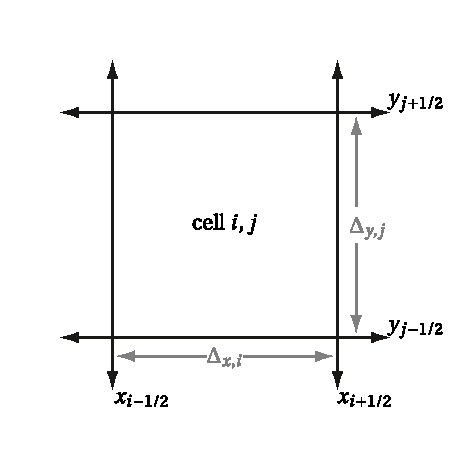
\includegraphics{cell-diagram}
  \caption{Diagram of cell $i,j$.}
  \label{fig:cellDiagram}
\end{figure}

To preserve particles, it's necessary that $F_T^y$ from cell $i,j$ is equal to
$F_B^y$ from cell $i,{j+1}$, and the same from the other directions.

%%%%%%%%%%%%%%%%%%%%%%%%%%%%%%%%%%%%%%%%%%%%%%%%%%%%%%%%%%%%%%%%%%%%%%%%%%%%%%%%
\section{Neglecting transverse diffusion}

Perhaps the simplest way to discretize the anisotropic diffusion equation is by
neglecting the off-diagonal terms of the diffusion tensor that imply transverse
leakage.

In certain simple problems, this is not an approximation. As long as the
opacity is invariant with respect to one of the coordinate system's axes, the
transport solution for $f$ will only change along one axis, and the
off-diagonal terms are zero. Larsen and Trahan's VHTR test problem
\cite{Lar2009c} is an example of such a geometry.

%%%%%%%%%%%%%%%%%%%%%%%%%%%%%%%%%%%%%%%%%%%%%%%%%%%%%%%%%%%%%%%%%%%%%%%%%%%%%%%%
\section{Gol'din-style discretization}

\cite{Val2002}

\begin{figure}[htb]
  \centering
  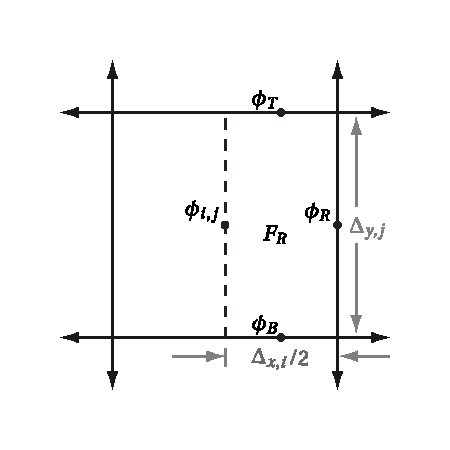
\includegraphics{goldin-righthalf}
  \caption{Right half of cell $i,j$.}
  \label{fig:goldinRight}
\end{figure}

%%%%%%%%%%%%%%%%%%%%%%%%%%%%%%%%%%%%%%%%%%%%%%%%%%%%%%%%%%%%%%%%%%%%%%%%%%%%%%%%
\section{Nine-point stencil}

Fig.~\ref{fig:cellAnisoLeakage} shows the leakage out of cell $i,j$ through the
right face.
\begin{figure}[htb]
  \centering
  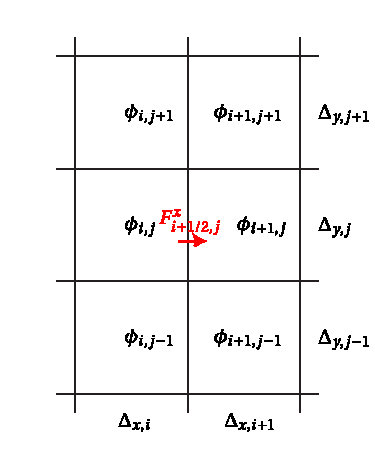
\includegraphics{cell-leakage-right}
  \caption{Diagram showing the radiation exiting interior cell $i,j$ through the
  right face.}
  \label{fig:cellAnisoLeakage}
\end{figure}
We evaluate the face-averaged normal component of the flux,
$F_{i+1/2,j}^x \equiv \int_{y_{j-1/2}}^{y_{j+1/2}} \vec{F} \vd \vec{n} \ud
y$, from both cell $i,j$ and cell $i+1,j$, and set them equal to each other.
Solving for $F_{i+1/2,j}^x$ gives
\begin{equation} \label{eq:cellAnisoFlux}
  F_{i+1/2,j}^{x} \approx
  - \frac{D^{xx}_{i+1/2,j}}{\Delta_{x,i+1/2}}
  \left[ 
    \left( \phi_{i+1,j} - \phi_{i,j} \right)
  + \frac{D^{xy}_{i,j}/D^{xx}_{i,j}}{2/\Delta_{x,i}}
    \pder{\phi}{y} \Bigg|_{x_{i+1/2}^-}
  + \frac{D^{xy}_{i+1,j}/D^{xx}_{i+1,j}}{2/\Delta_{x,i+1}}
    \pder{\phi}{y} \Bigg|_{x_{i+1/2}^+}
  \right]
\end{equation}
where $\tpder{\phi}{y} |_{x_{i+1/2}^-}$ is the transverse derivative of
$\phi$ on the left side of the face, and $\tpder{\phi}{y} |_{x_{i+1/2}^+}$ is
the transverse derivative as viewed from the right side of the face.
The harmonic-averaged diffusion coefficient is
\begin{equation} \label{eq:cellEdgeDHarmonic}
  \frac{D^{xx}_{i+1/2,j}}{\Delta_{x,i+1/2}} \equiv \left[
  \frac12 \left( \frac{D^{xx}_{i,j}}{\Delta_{x,i}} \right)\inv
 + \frac12 \left( \frac{D^{xx}_{i+1,j}}{\Delta_{x,i+1}} \right)\inv
  \right]\inv\,.
\end{equation}

If $D^{xy}$ were zero for both cells, and $D^{xx}=D^{yy}$,
Eq.~\eqref{eq:cellAnisoFlux} would reduce to
the standard cell-centered finite difference discretization so well known to
nuclear engineering students.

Now, in our first nine-point stencil, we approximated
\begin{equation*}
  \pder{\phi}{y} \Bigg|_{x_{i+1/2}^-} \approx \frac{\phi_{i,j+1} -
  \phi_{i,j-1}}{\tfrac12 \Delta_{y,j+1} + \Delta_{y,j} + \tfrac12
  \Delta_{y,j-1}}
\end{equation*}
in the interior of the problem and discarded the term near the boundaries. (The 
$\tpder{\phi}{y} |_{x_{i+1/2}^+}$ term is the same but replacing $i\to i+1$.)
An improvement is to approximate the case on the top boundary with
\begin{equation*}
  \pder{\phi}{y} \Bigg|_{x_{i+1/2}^-} \approx \frac{\phi_{i,j} -
  \phi_{i,j-1}}{\tfrac12 \Delta_{y,j} + \tfrac12 \Delta_{y,j-1} }
\end{equation*}
and the case on the bottom boundary with 
\begin{equation*}
  \pder{\phi}{y} \Bigg|_{x_{i+1/2}^-} \approx \frac{\phi_{i,j+1} -
  \phi_{i,j}}{\tfrac12 \Delta_{y,j+1} + \tfrac12 \Delta_{y,j} }
\end{equation*}

We can also approximate this derivative with approximate cell-edge values. In
the finite difference method, an intermediate cell-edge $\phi$ helps represent
the slope normal to the edge. It is eliminated in the process of finding
$\vec{F}\vd\vec{n}$, but if there is no transverse term, it is possible to
solve for the cell-edge $\phi$ in terms of the two cell-centered $\phi$. Let us
consider the finite difference approximation coupling two cells:
\begin{equation*}
  F = - D_0 \frac{\phi_{1/2} - \phi_0}{\Delta_0/2}
  \qquad\text{and}\qquad
  F = - D_1 \frac{\phi_{1} - \phi_{1/2}}{\Delta_1/2}\,.
\end{equation*}
Multiplying the left equation by $\Delta_0 / D_0$ and the right equation by
$\Delta_1 / D_1$,
\begin{equation*}
  -\frac{\Delta_0/2}{D_0 } F = \phi_{1/2} - \phi_0
  \qquad\text{and}\qquad
  -\frac{\Delta_1/2}{D_1 } F = \phi_{1} - \phi_{1/2}
\end{equation*}
adding them eliminates gives the standard finite-difference approximation for $F$,
\begin{equation*}
  F = - \left( \frac{\Delta_0/2}{D_0 } + \frac{\Delta_1/2}{D_1 } \right)\inv
  \left( \phi_1 - \phi_0 \right),
\end{equation*}
and subtracting the second from the first gives
\begin{equation*}
 -\frac{\Delta_0/2}{D_0 }F + \frac{\Delta_1/2}{D_1 } F
 = 2 \phi_{1/2}-(\phi_0+\phi_1)\,.
\end{equation*}
Defining $ d_i \equiv \frac{\Delta_i}{D_i}$ for $i=0,1$ for brevity, then
\begin{equation*}
  \frac12 F (d_1 - d_0)
 = 2 \phi_{1/2}-(\phi_0+\phi_1)
  \qquad\text{and}\qquad
 F = -2\left( d_1 + d_0 \right)\inv (\phi_1 - \phi_0)\,.
\end{equation*}
Substituting $F$ into the left equation,
\begin{align*}
  \left( d_1 + d_0 \right)\inv\left(d_1 - d_0\right) (\phi_1 - \phi_0)
  &= 2 \phi_{1/2}-(\phi_0+\phi_1)
  \\
 \frac12 \left[ 1 - \frac{d_1 - d_0}{d_1 + d_0} \right] \phi_1
+ \frac12 \left[ 1 + \frac{d_1 - d_0}{d_1 + d_0} \right] \phi_0
 &= \phi_{1/2}
  \\
 \frac{d_0}{d_1 + d_0} \phi_1
+ \frac{d_1}{d_1 + d_0} \phi_0
 &= \phi_{1/2}\,.
\end{align*}

For our case in anisotropic diffusion, we want to approximate 
\begin{equation*}
  \pder{\phi}{y} \Bigg|_{x_{i+1/2}^-} \approx \frac{\phi_{i,j+1/2} -
  \phi_{i,j-1/2}}{\Delta_{y,j}} \,.
\end{equation*}
In evaluating these cell-edge $\phi$ we neglect the transverse leakage (as
leaving them in would add unknowns on more cell faces) and apply the previous
result:
\begin{equation*}
  \phi_{i,j+1/2} \approx
  \frac{D_{i,j}^{yy} / \Delta_{y,j}}{D_{i,j+1}^{yy} / \Delta_{y,j+1} +
  D_{i,j}^{yy} / \Delta_{y,j}} \phi_{i,j+1}
+ \frac{D_{i,j+1}^{yy} / \Delta_{y,j+1}}{D_{i,j+1}^{yy} / \Delta_{y,j+1} +
D_{i,j}^{yy} / \Delta_{y,j}} \phi_{i,j} \,.
\end{equation*}
Subtracting one from the $j$ indices gives the corresponding equation for the
bottom face:
\begin{equation*}
  \phi_{i,j-1/2} \approx
  \frac{D_{i,j-1}^{yy} / \Delta_{y,j-1}}{D_{i,j}^{yy} / \Delta_{y,j} +
  D_{i,j-1}^{yy} / \Delta_{y,j-1}} \phi_{i,j}
+ \frac{D_{i,j}^{yy} / \Delta_{y,j}}{D_{i,j}^{yy} / \Delta_{y,j} +
D_{i,j-1}^{yy} / \Delta_{y,j-1}} \phi_{i,j-1} \,.
\end{equation*}
If cell $i,j$ is in the interior, 
\begin{equation*}
  \pder{\phi}{y} \Bigg|_{x_{i+1/2}^-} \approx \frac{\phi_{i,j+1/2} -
  \phi_{i,j-1/2}}{\Delta_{y,j}} \,,
\end{equation*}
or if it is on the top boundary,
\begin{equation*}
  \pder{\phi}{y} \Bigg|_{x_{i+1/2}^-} \approx \frac{\phi_{i,j} -
  \phi_{i,j-1/2}}{\Delta_{y,j} / 2} \,,
\end{equation*}
or if it is on the bottom boundary,
\begin{equation*}
  \pder{\phi}{y} \Bigg|_{x_{i+1/2}^-} \approx \frac{\phi_{i,j+1/2} -
  \phi_{i,j}}{\Delta_{y,j} / 2} \,.
\end{equation*}

If the anisotropic diffusion coefficients are homogeneous and the grid is
uniform, this expression for $\tpder{\phi}{y}$ is exactly equivalent to the
simpler one.

\begin{figure}[htb]
  \centering
  %\hspace{-.6in}
  \subfigure[Diagonal-only anisotropic]{
  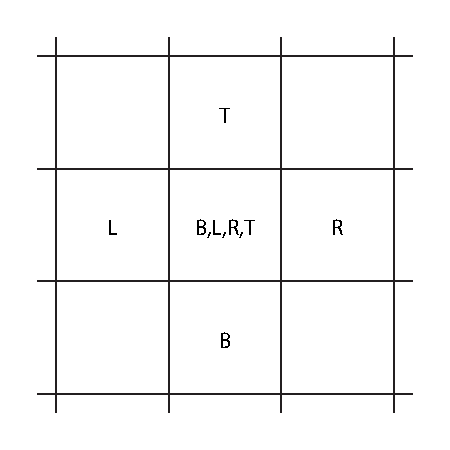
\includegraphics{diaganiso-leakage-terms}
  }
  %\hspace{-.2in}
  \subfigure[Cell anisotropic]{
  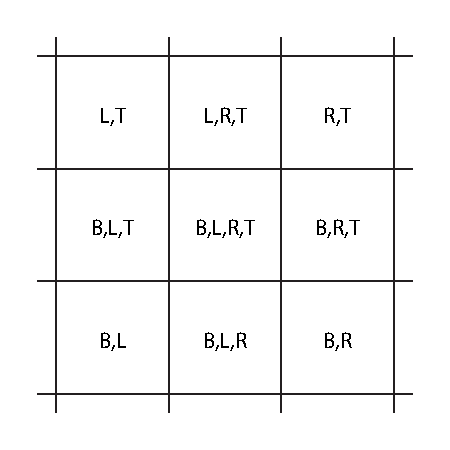
\includegraphics{cellaniso-leakage-terms}
  }
  %\hspace{-.6in}
  \caption{Stencils for $- \grad \vd \Dtens \grad \phi$ showing contribution
  from the leakage terms of each face of the center cell.}
  \label{fig:anisoStencils}
\end{figure}



% !TEX root = _individual/flatland.tex

%%%%%%%%%%%%%%%%%%%%%%%%%%%%%%%%%%%%%%%%%%%%%%%%%%%%%%%%%%%%%%%%%%%%%%%%%%%%%%%%
\chapter{Flatland Geometry}\label{chap:flatland}

``Flatland'' is a fictional two-dimensional universe in which particles are
constrained to exist and
travel in a 2-D plane \cite{Asa2008}. Because the flatland phase space is
$(x,y,\omega)$ with \emph{one} angular variable (the azimuthal~$\omega$),
rather than the
standard 2-D $(x,y,\mu,\omega)$ with \emph{two} angular variables (the
polar cosine~$\mu$ and the azimuthal~$\omega$),
flatland is a computationally simpler testing ground that retains the
complexity of multidimensional geometry. For this reason, flatland has recently
been used in the development and testing of multi-D transport methods, including
the new anisotropic diffusion method \cite{Lar2009c,Joh2011,Tra2011}.

Previous work has shown that the 3-D diffusion coefficient
$\frac{1}{3\sigma}$ differs from the flatland diffusion coefficient
$\frac{1}{2\sigma}$, but accurate boundary conditions for the flatland
diffusion equations have not been derived. An accurate diffusion
boundary condition is needed for benchmarking new transport methods, such as
anisotropic diffusion, against
diffusion solutions. Thus, in this chapter we derive ``Marshak''
and ``variational'' boundary conditions for the flatland diffusion equation.
We also present Monte Carlo sampling algorithms tailored to flatland
geometry, as well as a quick description of how 2-D \SN\ transport can easily be
adapted to flatland.

These methods are implemented in flatland primarily for the purpose of
comparison with the new anisotropic diffusion methods. We briefly derive the
AD approximation in flatland geometry for use in our benchmark problems.

%For the purposes of comparison, we also consider Fig.~\ref{fig:chordFlatland} as
%a sagittal view of an infinite cylinder; Fig.~\ref{fig:chordRz} shows a
%cross-sectional view.
%
%\begin{figure}[htb]
%  \centering
%  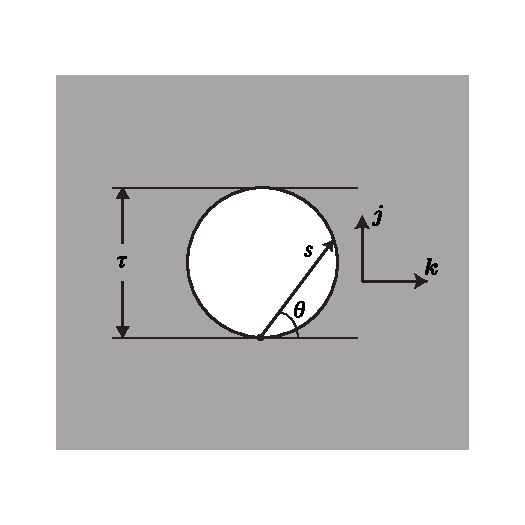
\includegraphics{chord-rz}
%  \caption[A cross-section of the chord length problem in cylindrical
%  geometry.]%
%  {A cross-section of the chord length problem in cylindrical
%  geometry. The orthogonal view looks like Fig.~\ref{fig:chordFlatland}.}
%  \label{fig:chordRz}
%\end{figure}

%%%%%%%%%%%%%%%%%%%%%%%%%%%%%%%%%%%%%%%%%%%%%%%%%%%%%%%%%%%%%%%%%%%%%%%%%%%%%%%%
\clearpage
\section{Transport}

To briefly illustrate the difference between flatland and 2-D geometry, we
view an infinite gap between two materials. The flatland problem and the
two-dimensional projection are identical, shown in Fig.~\ref{fig:chordFlatland}.
%
\begin{figure}[htb]
  \centering
  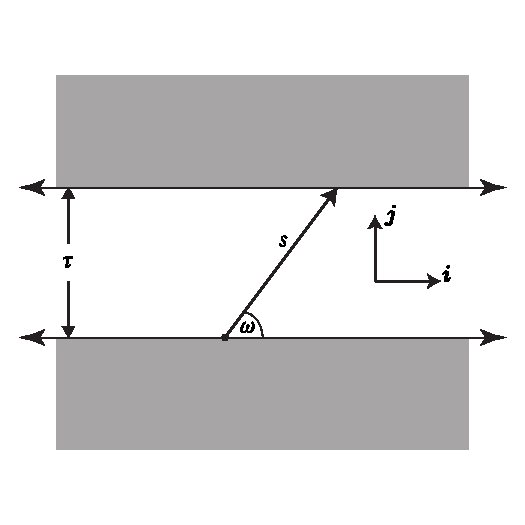
\includegraphics{chord-flatland}
  \caption[The infinite gap as represented on paper.]%
  {The infinite gap as represented on paper. The gap is a distance
  $\tau$ across, $\omega$ is the azimuthal angle, and $s$ is the
  distance across the gap.}
  \label{fig:chordFlatland}
\end{figure}
%
However, in the 2-D case, the figure is merely a slice of a three-dimensional
problem where the two gray rectangles and the gap are infinite in extent
(Fig.~\ref{fig:chordXy}). In the flatland case, the polar angle $\theta$ is
effectively fixed at $\theta=\pi/2$, i.e., $\mu=\cos\theta = 0$.
%
\begin{figure}[htb]
  \centering
  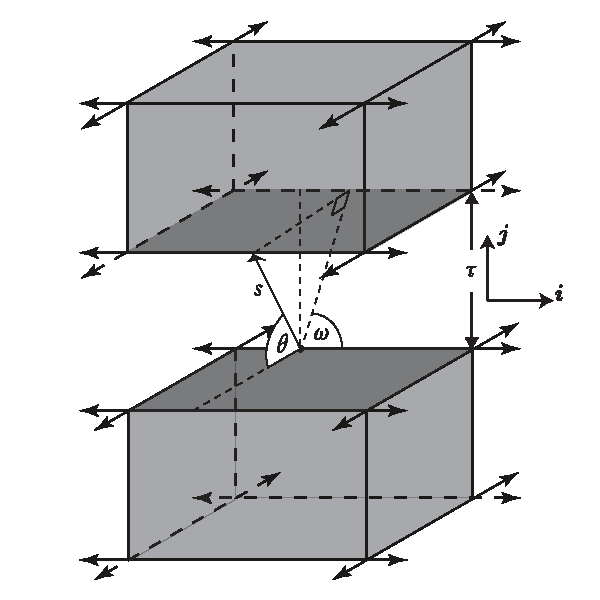
\includegraphics{chord-xyz}
  \caption[A 3-D view of the ``2-D'' infinite gap.]%
  {A 3-D view of the ``2-D'' infinite gap.
  The polar angle cosine is $\mu= \cos \theta$, and the azimuthal angle is
  $\omega$.}
  \label{fig:chordXy}
\end{figure}

Because the time-dependent and nonlinear terms of thermal radiative transfer are
not affected by the choice of geometry, we constrain our discussion in this
section to steady-state transport. Our application of the flatland
transport equation
has only isotropic emission (and ``pseudo-scattering'' if the linearized
transport equation is used), so we limit our study to the case of isotropic
scattering.

To begin, we write the steady-state transport equation with isotropic scattering
in a ``general geometry'' form valid both for flatland and real space (1-D,
2-D, and 3-D):
\begin{subequations} \label{eqs:ssTransport}
\begin{equation}\label{eq:ssTransportVol}
  \vec{\Omega}\vd \grad I(\vec{x}, \vec{\Omega})
  + \sigma(\vec{x}) I(\vec{x}, \vec{\Omega})
  = \frac{c(\vec{x}) \sigma(\vec{x})}{\gamma_0} \phi(\vec{x})
  + \frac{1}{\gamma_0} q(\vec{x}) \,,
  \quad \vec{x} \in V \,,\ \vec{\Omega} \in S\,.
\end{equation}
Here, we use the following definitions:
\begin{align*}
  I(\vec{x},\vec{\Omega}) &= \text{the steady-state angular intensity,} \\
  \vec{\Omega} &= \text{the unit direction vector,} \\
  S &= \text{the domain of the direction vector (the ``unit sphere''),} \\
  \gamma_n &= \text{the $n$th angular moment,} \\
  c(\vec{x}) &= \text{the scattering ratio, and} \\
  \phi(\vec{x}) &= \text{the scalar intensity, i.e.~the zeroth angular moment of $I$.}
\end{align*}
The direction vectors $\vec{\Omega}$ and domains $S$ are presented in
Table~\ref{tab:angularDomain}, and the moments $\gamma_0$ are evaluated in
Table~\ref{tab:angularMoments}. The specified incident radiation
boundary:
\begin{equation} \label{eq:ssBndy}
  I(\vec{x}, \vec{\Omega}) = I^b(\vec{x}, \vec{\Omega})
  \quad \vec{x} \in \partial V \,,\ \vec{\Omega} \vd \vec{n} < 0\,.
\end{equation}
\end{subequations}

\begin{table}[htb]
  \centering
  \begin{tabular}{rccc}
\toprule
   Geometry & $\vec{\Omega}$ & Domain $S$ & $\ud\Omega$
\\ \midrule
   1-D & $\mu$ & $-1 \le \mu \le 1$ & $\ud\mu$
   \\
   2-D & $\sqrt{1-\mu^2} \cos \omega \vec{i}
   + \sqrt{1-\mu^2} \sin \omega \vec{j}$
   & $-1 \le \mu \le 1$, $0 \le \omega < 2\pi$ & $\ud\mu \ud \omega$
   \\
   Flatland & $\cos \omega \vec{i} + \sin \omega \vec{j}$
   & $0 \le \omega < 2\pi$ & $\ud \omega$
   \\
   3-D & $\mu \vec{i}
   + \sqrt{1-\mu^2} \cos \omega \vec{j}
   + \sqrt{1-\mu^2} \sin \omega \vec{k}$
   & $-1 \le \mu \le 1$, $0 \le \omega < 2\pi$ & $\ud\mu \ud \omega$
\\ \bottomrule
  \end{tabular}
  \caption{Angular variables in the various geometries.}
  \label{tab:angularDomain}
\end{table}

\begin{table}[htb]
  \centering
  \begin{tabular}{rccc}
\toprule
   Geometry
   & $\gamma_0 \equiv \int_S \ud\Omega$
   & $\gamma_1 \equiv \int_S \abs{\vec{\Omega}\vd\vec{i}} \ud\Omega$
   & $\gamma_2 \equiv \int_S (\vec{\Omega}\vd\vec{i})^2 \ud\Omega$
\\ \midrule
   1-D & 2 & 1 & $\frac{2}{3}$
   \\
   2-D & $4\pi$ & $2\pi$ & $\frac{4\pi}{3}$
   \\
   Flatland & $2\pi$ & $4$ & $\pi$
   \\
   3-D & $4\pi$ & $2\pi$ & $\frac{4\pi}{3}$
\\ \bottomrule
  \end{tabular}
  \caption{Angular moments in each geometry.}
  \label{tab:angularMoments}
\end{table}

The ``unit sphere''---%
the domain of the unit direction $\vec{\Omega}$---%
differs among the geometries. In 3-D, the direction variable is a unit vector,
$\norm{\vec{\Omega}}=1$, so valid angles
lie on the surface of a sphere of unit radius. In 2-D, those angles are
projected onto a slice through the sphere's middle, so that
$\norm{\vec{\Omega}} \le 1$: valid angles are on a unit disc. Angles on the edge
of the disc---the unit circle---represent particles traveling along the slice,
and angles inside the unit circle are the projection of 3-D angles traveling with a
non-zero polar angle cosine. Flatland geometry allows only angles on the unit
circle, $\norm{\vec{\Omega}}=1$.

%%%%%%%%%%%%%%%%%%%%%%%%%%%%%%%%%%%%%%%%
\subsection{Monte Carlo sampling}

In numerically testing the anisotropic diffusion approximation, we use Monte Carlo
methods to generate the reference solutions.
The Monte Carlo method approximates the transport equation by tracking the
random histories of statistically large numbers of particles as they traverse a
problem. The behavior during their lifetime depends on probability distribution
functions (PDFs) that describe how they are born, how far they travel without a
collision, how they behave when they collide, and so on \cite{Lew1984,Bro2004a}.

In this section, we form and discuss the probability distributions particular to
flatland geometry. We briefly derive those PDFs,
integrate them to get cumulative distribution functions
(CDFs), and use the direct inversion method to show how a uniformly sampled
pseudo-random number $\xi \in [0,1)$ may be used to determine particle behavior
in flatland. Because the geometry tracking routines of steady state Monte Carlo
and Fleck and Cummings' IMC are identical, the results in this section are
applicable any flatland Monte Carlo implementation.

\subsubsection{Isotropic volume source}
A particle emitted from an isotropic internal source, whether an extraneous
radiation source or an indirect isotropic scattering event, has an equal
probability of entering any angle. In any geometry, the normalized PDF that
represents this process is
\begin{equation*}
  f(\vec{\Omega}) \ud\Omega = \alpha \ud\Omega \,,
  \quad \vec{\Omega} \in S \,,
\end{equation*}
where $\Omega$ is the angular domain of the
geometry (see Table~\ref{tab:angularDomain}), and $\alpha$ is a normalization
constant.
Requiring the PDF to integrate to unity over its domain gives the
following value for $\alpha$ in any geometry:
\begin{align*}
  1 = \int_{\Omega} f(\vec{\Omega}) \ud\Omega
  = \alpha \int_{\Omega} \ud\Omega = \alpha \gamma_0
  \lra
  \alpha = \frac{1}{\gamma_0}\,.
\end{align*}
Thus the angular distribution of an isotropic volume source is
\begin{equation}\label{eq:volumeSourcePdf}
  f(\vec{\Omega}) \ud\Omega = \frac{\ud\Omega}{\gamma_0} \,,
  \quad \vec{\Omega} \in S\,.
\end{equation}

In 2-D, using the identities from Tables~\ref{tab:angularDomain}
and~\ref{tab:angularMoments}, Eq.~\eqref{eq:volumeSourcePdf} evaluates to the
familiar
\begin{equation*}
  f(\mu,\omega) \ud\mu\ud\omega = \frac{\ud\mu\ud\omega}{4\pi} 
  = \frac{\ud\mu}{2}\frac{\ud\omega}{2\pi}
  \,,
  \quad -1\le \mu \le 1,\ 0 \le \omega < 2\pi\,,
\end{equation*}
which, integrated, yields the separable CDF
\begin{equation*}
  F(\mu,\omega) = F_1(\mu) F_2(\omega)
  = \frac{1 + \mu}{2}\frac{\omega}{2\pi}\,,
  \quad -1\le \mu \le 1,\ 0 \le \omega < 2\pi\,.
\end{equation*}
Setting two uniformly sampled random numbers $\xi_1 = F_1(\mu)$ and
$\xi_2 = F_2(\omega)$, solving for $\mu$ and $\omega$, and
introducing them back into the 2-D representation of $\vec{\Omega}$, we obtain the
new direction for an isotropically emitted particle in 2-D:
\begin{align*}
  \vec{\Omega} &= \sqrt{1-\mu^2} \cos \omega \vec{i}
  + \sqrt{1-\mu^2} \sin \omega \vec{j}
\\
  &= \sqrt{1-(2\xi_1-1)^2} \cos(2\pi\xi_2) \vec{i}
  + \sqrt{1-(2\xi_1-1)^2} \sin(2\pi\xi_2) \vec{j}\,.
\end{align*}

In flatland, Eq.~\eqref{eq:volumeSourcePdf} becomes the simpler
\begin{equation*}
  f(\omega) \ud\omega = \frac{\ud\omega}{2\pi} \,,
  \quad 0 \le \omega < 2\pi\,,
\end{equation*}
yielding the CDF
\begin{equation}\label{eq:volumeSourceFlatland}
  F(\omega) = \frac{\omega}{2\pi}\,,
  \quad 0 \le \omega < 2\pi\,,
\end{equation}
Setting $\xi_1 = F(\omega)$ and solving for $\omega = F\inv(\xi_1)$ gives the
following simple relation between an isotropically sampled angle $\omega$ and a
uniformly sampled random number $\xi_1$:
\begin{equation*}
  \omega = 2\pi \xi_1\,.
\end{equation*}
The flatland particle's new angle is therefore
\begin{equation*}
  \vec{\Omega} = \cos \omega \vec{i} + \sin \omega \vec{j}
  = \cos(2\pi\xi_1) \vec{i} + \sin(2\pi\xi_1) \vec{j}\,.
\end{equation*}

With only one independent variable that needs sampling, and the omission of
the transcendental operation $\sqrt{1-\mu^2}$, the computational cost of a
scattering event is less in flatland than in 2-D, leading to
faster simulation times.

\subsubsection{Isotropic surface source}\label{sec:isoSurface}
Particles emitted from an isotropic surface source have a cosine distribution
\cite{Gre2002}, where the partial first moment in each differential angle is
constant. The PDF for a surface source is
\begin{equation*}
  f(\vec{\Omega}) \ud\Omega = \alpha \abs{\vec{\Omega}\vd \vec{n}} \ud\Omega \,,
\quad \vec{\Omega}\vd \vec{n} < 0 \,,
\end{equation*}
where $\alpha$ is a normalization constant. We obtain $\alpha$ by integrating over
the angular domain and substituting the angular moments from Table~\ref{tab:angularMoments}:
\begin{align*}
  1 &= \int_{\vec{\Omega}\vd \vec{n} < 0} \left[ \alpha \abs{\vec{\Omega}\vd
  \vec{n}} \right] \ud\Omega
  \\
  1 &=\frac{\alpha}{2} \int_{\Omega} \abs{\vec{\Omega}\vd \vec{n}} \ud\Omega
  \\
  \alpha &= \frac{2}{\gamma_1}\,.
\end{align*}
Thus, the normalized PDF for an isotropic surface source is
\begin{equation}\label{eq:surfaceSourcePdf}
  f(\vec{\Omega}) \ud\Omega = \frac{2}{\gamma_1} \abs{\vec{\Omega}\vd \vec{n}} \ud\Omega \,,
\quad \vec{\Omega}\vd \vec{n} < 0 \,.
\end{equation}

In 3-D, choosing $\vec{n}=\vec{i}$, the isotropic surface PDF is
\begin{equation*}
  f(\mu,\omega) \ud\mu \ud\omega
  = \frac{1}{\pi} \mu \ud\mu \ud\omega
  = (2 \mu \ud\mu) \frac{\ud\omega}{2\pi}\,,
\end{equation*}
which gives the separable CDF
\begin{equation*}
  F(\mu,\omega) = \mu^2 \frac{\omega}{2\pi}\,.
\end{equation*}
The sampled directions are thus $\mu=\sqrt{\xi_1}$ and $\omega=2\pi \xi_2$.

In flatland, the surface source distribution is different. Let us choose
$\vec{n} = -\vec{j}$ so that emitted particles have azimuthal angles in the range
$\omega \in [0, \pi)$.
Applying the flatland identities in Tables~\ref{tab:angularDomain}
and~\ref{tab:angularMoments} to Eq.~\eqref{eq:surfaceSourcePdf}, we obtain
the following surface source PDF for flatland:
\begin{equation*}
  f(\omega) \ud\omega = \frac{2}{4} \, \abs{ -\sin \omega}\ud\omega
  = \frac{1}{2} \sin \omega\ud\omega \,,\quad 0 \le \omega < \pi\,.
\end{equation*}
The corresponding CDF is
\begin{equation}\label{eq:surfaceSourceFlatland}
  F(\omega) = \frac{1}{2} \left( 1-\cos\omega \right)
  \,,\quad 0 \le \omega < \pi\,.
\end{equation}
Solving for $\omega = F\inv(\xi_1)$ gives the sampled azimuthal angle for a surface source
in flatland:
\begin{equation*}
  \omega = \cos\inv(1 - 2\xi_1)\,.
\end{equation*}
Finally, we insert this sampled angle into the flatland
direction vector $\vec{\Omega}$ and use the identity
$\cos^2 \omega + \sin^2 \omega = 1$ to reduce the number of transcendental
functions. Thus the sampled direction of a particle from an isotropic surface
source is:
\begin{align*}
  \vec{\Omega} &= \cos \omega \vec{i} + \sin \omega \vec{j} \\
  &=  \cos[ \cos\inv(1 - 2\xi_1) ] \vec{i} + \sin[ \cos\inv(1 - 2\xi_1) ] \vec{j} \\
  &= (1 - 2\xi_1) \vec{i} + \sqrt{1 - (1 - 2\xi_1)^2} \vec{j}\,.
\end{align*}

%%%%%%%%%%%%%%%%%%%%%%%%%%%%%%%%%%%%%%%%
\subsection{Discrete ordinates quadrature}\label{sec:flatlandQuadrature}

A standard practice in two-dimensional discrete ordinates (\SN) solvers is to
create a quadrature set with polar angles that encompass only the top half of a
unit sphere, $\mu>0$, and to modify the ordinate weights so that they sum to
$4\pi$
\cite{Zik1997}. Well-constructed quadrature sets will also correctly
integrate the spherical harmonic functions \cite{Rab2007} over the unit sphere.
The odd spherical harmonic functions will automatically integrate to zero, and
the even
functions are linear combinations of the even angular moments of
Table~\ref{tab:angularMoments}:
\begin{equation*}
  \gamma_n
  = \sum_{m=1}^{M} \abs{ \vec{\Omega}_m \vd \vec{i}}^n w_m
  = \int_S \abs{ \vec{\Omega}\vd\vec{i} }^n \ud\Omega \,,\ n\ \text{even}.
\end{equation*}
Most quadrature sets do not exactly integrate partial odd moments.

The most straightforward way to implement a \emph{flatland} \SN\
code with only isotropic scattering is to use an existing 2-D \SN\ code with a
special quadrature set
consisting of ordinates that have a single
polar angle $\mu=0$. Using a Chebyshev--Gauss quadrature of the first kind
\cite{Str1966a} for the azimuthal angles will preserve the flatland angular moments,
\begin{equation*}
  \gamma_n
  = \sum_{m=1}^{M} \sin^n \theta_m w_m
  = \int_{2\pi} \sin^n \theta \ud\theta\,,\ n\ \text{even} \,.
\end{equation*}
A quadrature set with $2M$ total ordinates (i.e., $M$ per two octants, the
standard nomenclature for discrete ordinates quadratures) will exactly integrate
the first $2M-1$ polynomials of $x=\sin \theta$. The procedure to calculate
a Chebyshev quadrature set for the first quadrant is:
\begin{enumerate}
  \item Solve for the roots of an $2M$-order Chebyshev polynomial of the first
    kind on $[-1,1]$. Discard the negative roots.
  \item Take the inverse sine of the positive roots. These $M$ roots are the
    ordinate directions $\theta_m$ in the first quadrant.
  \item Assign the uniform weight $w_m = \frac{\pi}{M}$.
\end{enumerate}
For ease of implementation, we normalized the quadrature weights so that they sum
to $4\pi$ instead of $2\pi$. This allows flatland quadrature sets to be used in
an existing 2-D discrete ordinates code, where the scattering kernel expects the
quadrature set to be normalized to $4\pi$. Table~\ref{tab:chebyQs} gives several
orders of the Chebyshev quadrature set with sixteen digits of precision; a more
extensive and computer-readable set of ordinates is available online at
\url{https://github.com/sethrj/PyTRT/blob/master/tools/python/qs/cgvalues2.json}.

\begin{table}[p]
  \centering\small%
\begin{minipage}[t]{3in}
\null% needed to align tops
\hspace{\stretch{1}}
\begin{tabular}{l@{}l} \toprule
\multicolumn{2}{c}{$N=2$, $w=\pi$ } \\ \midrule
$\omega_{0}$ & ${}=0.7853981633974483$ \\ \toprule
\multicolumn{2}{c}{$N=4$, $w=\pi / 2$ } \\ \midrule
$\omega_{0}$ & ${}=0.3926990816987241$ \\
$\omega_{1}$ & ${}=1.1780972450961724$ \\ \toprule
\multicolumn{2}{c}{$N=8$, $w=\pi / 4$ } \\ \midrule
$\omega_{0}$ & ${}=0.1963495408493621$ \\
$\omega_{1}$ & ${}=0.5890486225480862$ \\
$\omega_{2}$ & ${}=0.9817477042468103$ \\
$\omega_{3}$ & ${}=1.3744467859455345$ \\ \toprule
\multicolumn{2}{c}{$N=16$, $w=\pi / 8$ } \\ \midrule
$\omega_{0}$ & ${}=0.0981747704246810$ \\
$\omega_{1}$ & ${}=0.2945243112740431$ \\
$\omega_{2}$ & ${}=0.4908738521234052$ \\
$\omega_{3}$ & ${}=0.6872233929727672$ \\
$\omega_{4}$ & ${}=0.8835729338221293$ \\
$\omega_{5}$ & ${}=1.0799224746714915$ \\
$\omega_{6}$ & ${}=1.2762720155208536$ \\
$\omega_{7}$ & ${}=1.4726215563702156$ \\ \toprule
\multicolumn{2}{c}{$N=32$, $w=\pi / 16$ } \\ \midrule
$\omega_{0}$ & ${}=0.0490873852123405$ \\
$\omega_{1}$ & ${}=0.1472621556370216$ \\
$\omega_{2}$ & ${}=0.2454369260617026$ \\
$\omega_{3}$ & ${}=0.3436116964863836$ \\
$\omega_{4}$ & ${}=0.4417864669110647$ \\
$\omega_{5}$ & ${}=0.5399612373357457$ \\
$\omega_{6}$ & ${}=0.6381360077604268$ \\
$\omega_{7}$ & ${}=0.7363107781851078$ \\
$\omega_{8}$ & ${}=0.8344855486097889$ \\
$\omega_{9}$ & ${}=0.9326603190344699$ \\
$\omega_{10}$ & ${}=1.0308350894591509$ \\
$\omega_{11}$ & ${}=1.1290098598838318$ \\
$\omega_{12}$ & ${}=1.2271846303085130$ \\
$\omega_{13}$ & ${}=1.3253594007331939$ \\
$\omega_{14}$ & ${}=1.4235341711578751$ \\
$\omega_{15}$ & ${}=1.5217089415825562$ \\
\bottomrule
\end{tabular}%
\hspace{\stretch{1}}
\end{minipage}%
%
\begin{minipage}[t]{3in}
\null% needed to align tops
\hspace{\stretch{1}}
\begin{tabular}{l@{}l} \toprule
\multicolumn{2}{c}{$N=64$, $w=\pi / 32$ } \\ \midrule
$\omega_{0}$ & ${}=0.0245436926061703$ \\
$\omega_{1}$ & ${}=0.0736310778185108$ \\
$\omega_{2}$ & ${}=0.1227184630308513$ \\
$\omega_{3}$ & ${}=0.1718058482431918$ \\
$\omega_{4}$ & ${}=0.2208932334555323$ \\
$\omega_{5}$ & ${}=0.2699806186678729$ \\
$\omega_{6}$ & ${}=0.3190680038802134$ \\
$\omega_{7}$ & ${}=0.3681553890925539$ \\
$\omega_{8}$ & ${}=0.4172427743048944$ \\
$\omega_{9}$ & ${}=0.4663301595172349$ \\
$\omega_{10}$ & ${}=0.5154175447295755$ \\
$\omega_{11}$ & ${}=0.5645049299419159$ \\
$\omega_{12}$ & ${}=0.6135923151542565$ \\
$\omega_{13}$ & ${}=0.6626797003665970$ \\
$\omega_{14}$ & ${}=0.7117670855789375$ \\
$\omega_{15}$ & ${}=0.7608544707912781$ \\
$\omega_{16}$ & ${}=0.8099418560036186$ \\
$\omega_{17}$ & ${}=0.8590292412159591$ \\
$\omega_{18}$ & ${}=0.9081166264282996$ \\
$\omega_{19}$ & ${}=0.9572040116406402$ \\
$\omega_{20}$ & ${}=1.0062913968529807$ \\
$\omega_{21}$ & ${}=1.0553787820653211$ \\
$\omega_{22}$ & ${}=1.1044661672776617$ \\
$\omega_{23}$ & ${}=1.1535535524900022$ \\
$\omega_{24}$ & ${}=1.2026409377023428$ \\
$\omega_{25}$ & ${}=1.2517283229146832$ \\
$\omega_{26}$ & ${}=1.3008157081270237$ \\
$\omega_{27}$ & ${}=1.3499030933393643$ \\
$\omega_{28}$ & ${}=1.3989904785517049$ \\
$\omega_{29}$ & ${}=1.4480778637640452$ \\
$\omega_{30}$ & ${}=1.4971652489763858$ \\
$\omega_{31}$ & ${}=1.5462526341887264$ \\
\bottomrule
\end{tabular}%
\hspace{\stretch{1}}
\end{minipage}%
\caption[Chebyshev--Gauss flatland quadrature sets.]{Chebyshev--Gauss
  flatland quadrature sets. Orders 2, 4, 8, 16, 32, and 64 are given for the
  first quadrant. The weights in each order are equal and sum to $4\pi$.}
  \label{tab:chebyQs}
\end{table}

In order to demonstrate the effect of this weight renormalization, let us
consider the calculation of the anisotropic diffusion tensor
in a homogeneous medium.  The purely absorbing flatland transport problem has the
solution $f(\vec{\Omega}) = \frac{1}{2\pi\sigma}$, which yields the diffusion
coefficient
\begin{equation*}
  \Dtens = \int_{0}^{2\pi} \vec{\Omega}\vec{\Omega} f(\vec{\Omega}) \ud \omega
  = \frac{1}{2\sigma} \Identitytens \,.
\end{equation*}
In an \SN\ calculation implemented with modified quadrature weights, the
transport solution for each angle $m$ will yield $f_m = \frac{1}{4\pi\sigma}$,
and the quadrature integration will yield
\begin{equation*}
  \Dtens = \sum_{m=1}^{M} \vec{\Omega}_m \vec{\Omega}_m f_m  w_m 
  = \frac{1}{2\sigma} \Identitytens \,.
\end{equation*}
This implementation therefore will calculate correct low-order angular moments of
the transport solution, but the apparent value of each $f_m$ is one half 
the correct value. Thus, for example, visualizing the \SN\
solution by plotting $f_m$ as a function of $\omega_m$ requires multiplying by a
factor of two.

%%%%%%%%%%%%%%%%%%%%%%%%%%%%%%%%%%%%%%%%%%%%%%%%%%%%%%%%%%%%%%%%%%%%%%%%%%%%%%%%
\section{Diffusion}

An accurate flatland diffusion formulation
is needed for benchmarking the anisotropic diffusion
approximation against diffusion solutions.
In the following section we derive ``Marshak'' and ``variational'' boundary
conditions for the flatland diffusion equation. (A summary of this original
work is published in \cite{Joh2011a}.)
%There is no loss of generality in
%ignoring the time dependence because of the quasi-static approximation made in
%the derivation of the diffusion coefficient (see \S\ref{sec:bgDiffusion}).

The difference between diffusion in flatland and 2-D results from the
angular moments in the two geometries, which
are defined (and evaluated in Table~\ref{tab:angularMoments}) as:
\begin{equation*}
  \gamma_n \equiv \int_S \abs{\vec{\Omega} \vd \vec{i}}^n \ud\Omega\,.
\end{equation*}
These give rise not only to a different diffusion coefficient in the interior
but also different boundary conditions.

%%%%%%%%%%%%%%%%%%%%%%%%%%%%%%%%%%%%%%%%
\subsection{Interior diffusion approximation}

The diffusion approximation begins by assuming that $I$ is linear in angle:
\begin{equation*}
  I(\vec{x}, \vec{\Omega}) \approx f(\vec{x}) + \vec{\Omega} \vd
  \vec{g}(\vec{x})\,.
\end{equation*}
The zeroth angular moment of $I$ determines $f$:
\begin{equation*}
  \phi = \int_S I \ud\Omega
= \int_S \left( f + \vec{\Omega}\vd \vec{g} \right) \ud\Omega
= \int_S\ud\Omega f + 0
= \gamma_0 f \,,
\end{equation*}
and the first moment of $I$ determines $g$:
\begin{equation*}
  \vec{F} = \int_S \vec{\Omega} I \ud\Omega
= f \int_S \vec{\Omega} \ud\Omega
  + \vec{g} \vd \int_S \vec{\Omega}\vec{\Omega} \ud\Omega
= \gamma_2 \vec{g} \,.
\end{equation*}
This is the \Pone\ approximation to the radiation intensity:
\begin{equation}\label{eq:ssPone}
  I(\vec{x}, \vec{\Omega})
  \approx \frac{1}{\gamma_0} \phi(\vec{x})
  + \frac{1}{\gamma_2} \vec{\Omega} \vd \vec{F}(\vec{x})\,.
\end{equation}

The diffusion approximation is a closure for the first angular moment of
the transport equation. Operating on Eq.~\eqref{eq:ssTransportVol} by
$\int_S \vec{\Omega} (\cdot) \ud\Omega$ and substituting
the approximation in Eq.~\eqref{eq:ssPone} reduces the first angular moment of
the transport equation to the following:
\begin{align*}
  \grad \vd \int_S \vec{\Omega} \vec{\Omega} I
  \ud\Omega
  + \sigma \int_S \vec{\Omega} I \ud\Omega
  &=
  \frac{c\sigma}{\gamma_0} \phi \int_S \vec{\Omega} \ud\Omega
  + \frac{1}{\gamma_0} q \int_S \vec{\Omega} \ud\Omega
  \\
  \grad \vd \int_S \vec{\Omega} \vec{\Omega} \left(
  \frac{1}{\gamma_0}\phi + \frac{1}{\gamma_2} \vec{\Omega} \vd \vec{F}
  \right)
  \ud\Omega
  + \sigma \vec{F}
  &= 0
  \\
  \frac{1}{\gamma_0} \grad \vd \int_S \vec{\Omega} \vec{\Omega}
  \ud\Omega\, \phi 
  + \sigma \vec{F} &= 0
  \\
  \frac{\gamma_2}{\gamma_0} \grad \phi + \sigma \vec{F} &= 0 \,.
\end{align*}
Solving for $\vec{F}$ gives Fick's law, expressed in the general form:
\begin{equation} \label{eq:fickGeneral}
  \vec{F}(\vec{x})
  = - \frac{\gamma_2}{\gamma_0} \frac{1}{\sigma(\vec{x})} \grad \phi(\vec{x})
  \equiv -D(\vec{x}) \grad \phi(\vec{x})\,.
\end{equation}
In 2-D and 3-D, $\gamma_2/\gamma_0 = (4\pi / 3) / (4\pi) = 1/3$; in
flatland, $\gamma_2/\gamma_0 = \pi / (2\pi) = 1/2$. Thus, $D=\frac{1}{3\sigma}$ in
2-D but $D=\frac{1}{2\sigma}$ in flatland.

Substituting Fick's law into the linear-in-angle approximation,
Eq.~\eqref{eq:ssPone}, we obtain the diffusion approximation to the angular
intensity:
\begin{align} \nonumber
  I(\vec{x}, \vec{\Omega})
  &\approx \frac{1}{\gamma_0} \phi(\vec{x})
  + \frac{1}{\gamma_2} \vec{\Omega} \vd \left[ - \frac{\gamma_2}{\gamma_0}
  \frac{1}{\sigma(\vec{x})} \grad \phi(\vec{x}) \right]
  \\ \label{eq:diffusionIntensity}
  I(\vec{x}, \vec{\Omega})
  &= \frac{1}{\gamma_0} \left[ \phi(\vec{x})
  - \frac{1}{\sigma(\vec{x})}
  \vec{\Omega} \vd \grad \phi(\vec{x}) \right] \,.
\end{align}
In physical geometry this is the standard diffusion approximation
\begin{equation*}
 I(\vec{x}, \vec{\Omega})
= \frac{1}{4\pi} \left[ \phi(\vec{x}) - \frac{1}{\sigma(\vec{x})} \vec{\Omega}
\vd \grad \phi(\vec{x}) \right] \,,
\end{equation*}
and in flatland, the diffusion approximation is
\begin{equation}\label{eq:flatlandDiffusion}
 I(\vec{x}, \vec{\Omega})
= \frac{1}{2\pi} \left[ \phi(\vec{x}) - \frac{1}{\sigma(\vec{x})} \vec{\Omega}
\vd \grad \phi(\vec{x}) \right]\,.
\end{equation}

%%%%%%%%%%%%%%%%%%%%%%%%%%%%%%%%%%%%%%%%
\subsection{Marshak boundary condition}
The Marshak boundary condition \cite{Mar1947} preserves the incident radiation
flux (the partial first moment for incoming directions) on the boundary. It is
derived by substituting the approximate diffusion
intensity from Eq.~\eqref{eq:diffusionIntensity} into the boundary condition,
Eq.~\eqref{eq:ssBndy}, multiplying by $\abs{\vec{\Omega}\vd \vec{n}}$, and integrating over
incident directions:
\begin{align*}
\int_{\vec{\Omega}\vd \vec{n} < 0 } \abs{\vec{\Omega}\vd \vec{n}}
I^b \ud\Omega
 &= 
\int_{\vec{\Omega}\vd \vec{n} < 0 } \abs{\vec{\Omega}\vd \vec{n}} 
 \frac{1}{\gamma_0} \left[ \phi - \frac{1}{\sigma}
  \vec{\Omega} \vd \grad \phi \right]
  \ud\Omega
\\
F^{-}
&= 
\frac{1}{\gamma_0} \phi \left( \int_{\vec{\Omega}\vd \vec{n} < 0 }
\abs{\vec{\Omega}\vd \vec{n}} \ud\Omega \right) 
  - \frac{1}{\gamma_0}\frac{1}{\sigma}
  \left( \int_{\vec{\Omega}\vd \vec{n} < 0 } [-\vec{\Omega}\vd \vec{n}]
  \vec{\Omega} \ud\Omega  \right) \vd \grad \phi
\\
F^{-}
&=
\frac{1}{\gamma_0} \phi \left( \frac{\gamma_1}{2} \right) 
  + \frac{1}{\gamma_0}\frac{1}{\sigma} \left( \vec{n} \vd
  \frac{\gamma_2}{2} \Identitytens \right)
  \vd \grad \phi
\\
F^{-}
&=
\frac{\gamma_1}{2\gamma_0} \phi
+ \frac{\gamma_2}{2\gamma_0}\frac{1}{\sigma} \vec{n} \vd \grad \phi\,.
\end{align*}
This is the Marshak diffusion boundary condition:
\begin{equation} \label{eq:marshak}
\frac{2\gamma_0}{\gamma_1} F^{-}
=
\phi + \frac{\gamma_2}{\gamma_1}\frac{1}{\sigma} \vec{n} \vd \grad \phi\,.
\end{equation}

The value
\begin{equation*}
  \frac{\gamma_2}{\gamma_1}
  =
  \begin{cases}
    \frac{2}{3} \approx 0.6667 & \text{in 1-D, 2-D, 3-D; and} \\
    \frac{\pi}{4} \approx 0.7854 & \text{in flatland,}
  \end{cases}
\end{equation*}
is the Marshak extrapolation distance.
The underlying physical reason for the longer extrapolation distance in flatland
is that in 2-D, a greater fraction of particles travel at a steep angle to the
$x,y$-plane, yielding a steeper slope for $\phi$ on the boundary.

We can also rewrite the Marshak boundary condition in terms of the diffusion
coefficient by substituting $D$ from Eq.~\eqref{eq:fickGeneral}:
\begin{equation*}
\frac{2\gamma_0}{\gamma_1} F^{-}
= \phi + \frac{\gamma_0}{\gamma_1} D \vec{n} \vd \grad \phi\,.
\end{equation*}
In 1-D, 2-D, and 3-D geometries, this is the standard Marshak boundary condition
\begin{equation*}
4 F^{-}
= \phi + 2 D \vec{n} \vd \grad \phi\,.
\end{equation*}
In flatland, it is the following:
\begin{equation}\label{eq:flatMarshak}
\pi F^{-}
= \phi + \frac{\pi}{2} D \vec{n} \vd \grad \phi\,.
\end{equation}

%%%%%%%%%%%%%%%%%%%%%%%%%%%%%%%%%%%%%%%%
\subsection{Variational boundary condition} \label{sec:varBndy}
It is known that the Marshak boundary condition is heuristic and that
a more accurate boundary condition for diffusion can be derived from an
asymptotic matched boundary layer analysis. However, a simpler
method of deriving a more accurate (than Marshak) boundary condition is to use
a variational analysis \cite{Mal1991}.
A shorter but equivalent analysis, adapted to flatland geometry, follows.

%A lengthy asymptotic boundary layer
%matching analysis \cite{Hab1975} shows that the correct weighting of the
%boundary condition is not $\abs{\vec{\Omega}\vd\vec{n}}$ but rather
%$W(\abs{\vec{\Omega}\vd\vec{n}})$, where $W$ is related to Chandrasekhar's
%$H$-function \cite{Cha1960}:
%\begin{equation*}
%  W(\mu) = \frac{\sqrt{3}}{2} \mu H(\mu) \,,
%\end{equation*}
%which gives an extrapolation distance of
%\begin{align*}
%  z_0 = \frac{\int_{0}^{1} \mu W(\mu) \ud \mu}{\int_{0}^{1} W(\mu) \ud
%  \mu} \approx 0.7104\,.
%\end{align*}
%
%A variational analysis \cite{Mal1991} has been used to
%derive a very accurate approximation to $W$:
%\begin{equation*}
%W(\mu) \approx \mu + \tfrac{3}{2} \mu^2 \,,
%\end{equation*}
%which gives the approximate extrapolation distance of
%\begin{equation*}
%  z_0 = \frac{\int_{0}^{1} \mu (\mu + \tfrac{3}{2} \mu^2 ) \ud
%  \mu}{\int_{0}^{1} (\mu + \tfrac{3}{2} \mu^2 ) \ud \mu} 
%  = \frac{17}{24} \approx 0.7083 \,.
%\end{equation*}

We consider a homogeneous, source-free ($q=0$), purely scattering ($c=1$)
transport problem in a
semi-infinite flatland plane.\footnote{%
The justification for setting $c=1$ and $q=0$ relates to the asymptotic
scaling used to derive diffusion from the transport equation:
both $q$ and $1-c$ are $O(\epsilon^2)$ quantities \cite{Mal1991}.}
The transport equation~\eqref{eq:ssTransportVol} becomes
\begin{subequations} \label{eqs:flatTransport}
\begin{equation}\label{eq:flatTransportVol}
  \cos \omega \pder{I}{x} + \sin \omega \pder{I}{y} + \sigma I
  = \frac{\sigma}{2\pi} \int_{0}^{2\pi} I \ud \omega'\,,\quad
 -\infty < x < \infty,\ 0 \le y < \infty,\ 0 \le \omega < 2\pi\,.
\end{equation}
It has a uniform incident boundary condition,
\begin{equation}\label{eq:flatTransportBndy}
  I(x, 0, \omega) = I^b(\omega) \,,\quad -\infty < x < \infty,\ 
  0 \le \omega < \pi \,.
\end{equation}
\end{subequations}
%The justification for using a purely scattering problem is related to the
%asymptotic analysis that shows the transport solution to satisfy a diffusion
%equation in the ``diffusive'' limit. In this limit, absorption is scaled as
%$O(\epsilon^2)$; the full variational analysis \cite{Mal1991} yields a
%variational estimate of the transport solution also accurate to $O(\epsilon^2)$.

Because neither the boundary condition nor $\sigma$ varies
in $x$, $\tpder{I}{x}=0$, and Eq.~\eqref{eq:flatTransportVol} reduces to the
one-dimensional flatland transport equation 
\begin{equation*}
  \sin \omega \pder{}{y}I(y,\omega) + \sigma I(y,\omega)
  = \frac{\sigma}{2\pi} \int_{0}^{2\pi} I(y,\omega') \ud \omega'\,.
\end{equation*}
which is \emph{not} the 1-D planar geometry transport equation.

We define the $y$ components of the angular moments of $I$ as
\begin{equation} \label{eq:flatPhi}
  \phi_m(y) = \int_{0}^{2\pi} (\vec{\Omega}\vd\vec{j})^m I(y,\omega) \ud\omega
  = \int_{0}^{2\pi} (\sin\omega)^m I(y,\omega) \ud\omega \,.
\end{equation}
As $y\to\infty$, the intensity $I$ will approach a constant $\varphi/2\pi$,
which gives $\phi_0(\infty)=\phi(\infty)\equiv\varphi$.
Concordantly, $\phi_1(\infty)=0$.

Operating on the transport equation by $\int_{0}^{2\pi} (\sin\omega)^m (\cdot)
\ud\omega$ gives the $m$th angular moment in the $y$ direction:
\begin{align} \nonumber
  \pder{}{y} \int_{0}^{2\pi} (\sin\omega)^{m+1} I \ud\omega
  + \sigma \int_{0}^{2\pi} (\sin\omega)^{m} I \ud\omega
  &= \frac{\sigma}{2\pi} \int_{0}^{2\pi} I \ud \omega'
  \int_{0}^{2\pi} (\sin\omega)^{m} \ud\omega
  \\ \label{eq:flatMoments}
  \pder{\phi_{m+1}}{y}
  + \sigma \phi_{m}
  &= \frac{\sigma}{2\pi} \phi_{0}
  \int_{0}^{2\pi} (\sin\omega)^{m} \ud\omega\,.
\end{align}
For $m=0$, the conservation equation, Eq.~\eqref{eq:flatMoments} evaluates to
\begin{equation*}
  \pder{\phi_{1}}{y}
  + \sigma \phi_{0}
  = \frac{\sigma}{2\pi} \phi_{0} (2\pi)
  \lra
  \pder{\phi_{1}}{y} = 0\,.
\end{equation*}
In other words, the radiation flux is a constant, and because $\phi_1(\infty)=0$,
that constant is zero. Physically, a constant $\phi_1$ means that at every
point, the rate of energy being transferred away from the boundary is balanced
by energy moving toward the boundary. This logically follows from the lack of
absorption in the problem: at steady-state, the only means of energy loss is
through exiting the boundary.

Evaluating Eq.~\eqref{eq:flatMoments} for $m=1$ and using the result that
$\phi_{1}=0$, we obtain
\begin{equation*}
  \pder{\phi_{2}}{y}
  + \sigma \phi_{1}
  = \frac{\sigma}{2\pi} \phi_{0} (0)
  \lra
  \pder{\phi_{2}}{y} = 0\,.
\end{equation*}
Thus $\phi_{2}$ is also a constant. At large distances from the boundary,
$y\to\infty$, the radiation assumes an isotropic distribution,
$I\to\varphi/2\pi$. From these two facts we relate the second angular moment
throughout the problem to the equilibrium scalar intensity $\varphi$:
\begin{equation*}
  \phi_{2} = \int_{0}^{2\pi} (\sin\omega)^2 \frac{\varphi}{2\pi} \ud\omega
  = \frac{1}{2} \varphi\,.
\end{equation*}
% in 1-D, this would be $\int_{-1}^{1}\mu^2\frac{\varphi}{2} \ud \mu =
% \frac{1}{3} \varphi$.

Since $\phi_1=0$, we can add $\alpha \phi_1$ to the previous equation for any
$\alpha$:
\begin{align*}
 \alpha\phi_1 + \phi_{2} &= \frac{\varphi}{2} \\
 \int_{0}^{2\pi} (\alpha \sin\omega + \sin^2\omega)
 I(y,\omega) \ud\omega
 &= \frac{\varphi}{2}\,.
\end{align*}
At the boundary $y=0$, $I=I^b$ for incident angles $0 \le \omega < \pi$.
The variational analysis in \cite{Mal1991} reveals that certain trial functions
allow an exiting angular distribution that is isotropic to second order accuracy,
so we make the ``variational'' approximation that $I(0,\omega)=I^\text{out}$.
The previous equation then yields
\begin{equation*}
 \int_{0}^{\pi} (\alpha \sin\omega + \sin^2\omega)
 I^b(\omega) \ud\omega
 + \int_{\pi}^{2\pi} (\alpha \sin\omega + \sin^2\omega)\ud\omega I^\text{out}
 = \frac{\varphi}{2}\,.
\end{equation*}
The value $\alpha=\pi/4$ eliminates the integral over outgoing directions and
gives the following relation between moments of the incident angular flux and the
magnitude of the angular flux as $y\to\infty$:
\begin{equation}\label{eq:varBoundary}
 \varphi = 2\int_{0}^{\pi} \left( \frac{\pi}{4} \sin\omega + \sin^2\omega \right)
 I^b(\omega) \ud\omega
 \,.
\end{equation}

We wish our boundary condition to preserve the value of
$\varphi$ when the diffusion method is used, so we substitute the diffusion
approximation, Eq.~\eqref{eq:flatlandDiffusion}:
\begin{align*}
 \varphi &= 2\int_{0}^{\pi} \left( \frac{\pi}{4} \sin\omega + \sin^2\omega \right)
 I^b(\omega) \ud\omega
 \\
 &= 
  2\int_{0}^{\pi} \left( \frac{\pi}{4} \sin\omega + \sin^2\omega \right)
 \left( \frac{1}{2\pi} \phi -
  \frac{1}{\sigma} \sin\omega \pder{\phi}{y}\right)\ud\omega
\\
 &= 
\frac{1}{2\pi} \int_{0}^{\pi} \left( \frac{\pi}{2} \sin\omega + 2 \sin^2\omega
\right)\ud\omega
 \,\phi -
 \frac{1}{2\pi} \int_{0}^{\pi} \left( \frac{\pi}{2} \sin^2\omega + 2 \sin^3\omega \right)\ud\omega
  \,\frac{1}{\sigma} \pder{\phi}{y}
  \\
 &= 
 \frac{1}{2\pi} \left( \frac{\pi}{2} [2] + 2 \frac{\pi}{2}
\right) \phi
-
\frac{1}{2\pi} \left( \frac{\pi}{2} \left[ \frac{\pi}{2} \right] + 2 \left[
\frac{4}{3} \right] \right) \frac{1}{\sigma} \pder{\phi}{y}
\\
 &= 
  \phi
- \left( \frac{\pi}{8} + \frac{4}{3\pi} \right) \frac{1}{\sigma} \pder{\phi}{y}
\,.
\end{align*}
In this problem, the boundary surface outer normal is $\vec{n}=-\vec{j}$. 
Replacing $\sin \omega$ with $-\vec{\Omega}\vd\vec{n}$, we obtain the following
flatland variational boundary condition:
\begin{equation} \label{eq:flatVarBc}
\int_{\vec{\Omega}\vd\vec{n} < 0} \left[ \frac{\pi}{2}
\abs{\vec{\Omega}\vd\vec{n}} + 2 (\vec{\Omega}\vd\vec{n})^2 \right]
I^b(\vec{x}, \vec{\Omega}) \ud\Omega
= 
  \phi(\vec{x})
  - \left( \frac{\pi}{8} + \frac{4}{3\pi} \right) \frac{1}{\sigma}
  \vec{n}\vd\grad \phi(\vec{x})\,.
\end{equation}
Compared to the flatland Marshak boundary condition,
Eq.~\eqref{eq:flatMarshak}, the variational boundary condition not only yields a
different extrapolation distance $\frac{\pi}{8} + \frac{4}{3\pi} \approx
0.8171$ but also uses a different moment of the incident boundary flux.

%%%%%%%%%%%%%%%%%%%%%%%%%%%%%%%%%%%%%%%%
\subsection{Generalization}\label{sec:flatlandV}

Recall from the discussion of boundary conditions in
Chapter~\ref{chap:adDerivation} that to eliminate the boundary layer solution
in the interior of a 3-D problem, the necessary condition is
\begin{equation}\tagref{eq:tdKillBndy}
  \int_{\vec{\Omega}\vd\vec{n} < 0}
  W(\abs{\vec{\Omega}\vd\vec{n}}) \Ibl(\vec{x},\vec{\Omega}) \ud\Omega
  = 0\,,
  \quad \vec{x}\in \partial V ,\ \vec{\Omega}\vd \vec{n} < 0\,,
\end{equation}
where $W$ is related to Chandrasekhar's $H$-function \cite{Cha1960} and can be
approximated by a variationally-derived polynomial $W_2$:
\begin{equation} \tagref{eq:chandraW}
  W(\mu) = \frac{\sqrt{3}}{2} \mu H(\mu)
  \approx W_2(\mu) \equiv \mu + \tfrac{3}{2} \mu^2 \,, \quad 0 < \mu \le 1 \,.
\end{equation}
The exact extrapolation distance is the first moment of $W$:
\begin{equation*}
  z_0 = \int_{0}^{1} \mu W(\mu) \ud\mu
  \approx 0.7104\,,
\end{equation*}
and the variational approximation gives the following extrapolation distance:
\begin{equation*}
  z_0 \approx \int_{0}^{1} \mu W_2(\mu) \ud\mu = \tfrac{17}{24}
  \approx 0.7083\,.
\end{equation*}
Similarly, the 3-D Marshak boundary condition uses
\begin{equation*}
  W(\mu) \approx W_1(\mu) \equiv 2 \mu \,,
\end{equation*}
which gives the Marshak extrapolation distance
\begin{equation*}
  z_0 \approx \int_{0}^{1} \mu W_1(\mu) \ud\mu = \tfrac{2}{3}
  \approx 0.6667\,.
\end{equation*}

In our analysis of flatland boundary conditions, we have essentially been
investigating flatland equivalent of the $W$ function, which we term ``$V$'',
that preserves the interior solution of a flatland problem:
\begin{equation}\label{eq:flatKillBndy}
\int_{\vec{\Omega}\vd\vec{n} < 0} V( \abs{\vec{\Omega}\vd\vec{n}})
I^b(\vec{x}, \vec{\Omega}) \ud\Omega
=
\int_{\vec{\Omega}\vd\vec{n} < 0} V( \abs{\vec{\Omega}\vd\vec{n}})
I_\text{approx}(\vec{x}, \vec{\Omega}) \ud\Omega \,.
\end{equation}
The ``true'' function $V$ might be calculable, for example, by using a
flatland formulation of the $F_N$ method \cite{Sie1979}, but we instead used a
``variational'' analysis and the standard Marshak treatment to approximate $V$.

We define $V(\mu)$ on the domain $0 < \mu \le 1$, where for our purposes $\mu =
\abs{\vec{\Omega} \vd \vec{n}}$, and normalize the function and its
approximations so that in flatland geometry:
\begin{equation*}
  \int_{\vec{\Omega}\vd\vec{n} < 0} V( \abs{\vec{\Omega}\vd\vec{n}}) \ud\Omega
  = \int_{0}^{\pi} V(\sin\omega) \ud\omega
  = 1 \,.
\end{equation*}
The approximations to $V$ should also have this normalization. Analogous to the
$W$ function, the flatland extrapolation distance is the first moment of $V$:
\begin{equation*}
  z_0 = \int_{\vec{\Omega}\vd\vec{n} < 0} \abs{\vec{\Omega}\vd\vec{n}}
    V( \abs{\vec{\Omega}\vd\vec{n}}) \ud\Omega
  = \int_{0}^{\pi} V(\sin\omega) \sin\omega \ud\omega \,.
\end{equation*}

The flatland Marshak approximation uses only the first angular moment, which,
after normalization, is:
\begin{equation}\label{eq:flatV1}
  V_1(\mu) \equiv \frac{1}{2} \mu \,,
  \quad 0 < \mu \le 1 \,,
\end{equation}
giving the flatland extrapolation distance
\begin{equation*}
 z_0 = \int_{0}^{\pi} V_1(\sin\omega) \sin\omega \ud\omega
  = \frac{\pi}{4} \approx 0.7854 \,.
\end{equation*}

The variational analysis yielded the following two-term approximation to $V$:
\begin{equation}\label{eq:flatV2}
  V_2(\mu) \equiv \frac{1}{2} \mu + \frac{1}{\pi}\mu^2 \,,
  \quad 0 < \mu \le 1 \,.
\end{equation}
The resulting variational flatland extrapolation distance is:
\begin{equation*}
 z_0 = \int_{0}^{\pi} V_2(\sin\omega) \sin\omega \ud\omega
  = \frac{\pi}{8} + \frac{4}{3\pi} \approx 0.8171\,.
\end{equation*}

Using the variational $V(\mu)\approx V_2(\mu)$ with the diffusion
approximation, Eq.~\eqref{eq:flatlandDiffusion}, we obtain
Eq.~\eqref{eq:flatVarBc}. With the Marshak $V(\mu)\approx V_1(\mu)$, the result
is the less accurate Eq.~\eqref{eq:flatMarshak}.

%%%%%%%%%%%%%%%%%%%%%%%%%%%%%%%%%%%%%%%%%%%%%%%%%%%%%%%%%%%%%%%%%%%%%%%%%%%%%%%%
\section{Anisotropic diffusion}
The anisotropic diffusion method presented in
chapter~\ref{chap:adDerivation} needs little modification to be formulated
in the flatland geometry. The most notable change is in formulating the
low-order boundary conditions, which use the flatland function ``$V$'' rather
than the 3-D Chandrasekhar ``$W$.''

We begin with the time-dependent transport equation in the general-geometry
form,
\begin{subequations} \label{eqs:fadTransport}
\begin{multline} \label{eq:fadTransportVol}
  \frac{1}{c}\pder{I}{t}(\vec{x},\vec{\Omega},t)
  + \vec{\Omega}\vd \grad I(\vec{x},\vec{\Omega},t)
  + \sigma(\vec{x}) I(\vec{x},\vec{\Omega},t)
  \\ = \frac{\sigma_s(\vec{x})}{\gamma_0}
  \int_{S} I(\vec{x},\vec{\Omega}',t) \ud \Omega'
  + \frac{q(\vec{x},t)}{2\pi}
  \,, \quad \vec{x}\in V,\ \vec{\Omega}\in S,\ t \ge 0,
\end{multline}
with specified incident boundary conditions
\begin{equation} \label{eq:fadTransportBndy}
  I(\vec{x},\vec{\Omega},t) = I^b(\vec{x},\vec{\Omega},t) \,,
  \quad \vec{x}\in \partial V ,\ \vec{\Omega}\vd \vec{n} < 0,\ t > 0,
\end{equation}
and the initial condition
\begin{equation} \label{eq:fadTransportInit}
  I(\vec{x},\vec{\Omega},0) = I^i(\vec{x},\vec{\Omega}) \,,
  \quad \vec{x}\in V ,\ \vec{\Omega} \in S\,.
\end{equation}
\end{subequations}
In flatland, the unit sphere $S$ is $0 \le \omega < 2\pi$, $\Omega$ lives on
the unit circle, and $\gamma_0=2\pi$.

As before, we write the transport solution as a superposition of an interior
solution (far from initial conditions and exterior boundaries), a boundary layer
solution, and an initial layer solution.
\begin{equation}\tagref{eq:tdSuperposition}
  I(\vec{x},\vec{\Omega},t)
  \equiv \Iv(\vec{x},\vec{\Omega},t)
  + \Ibl(\vec{x},\vec{\Omega},t)
  + \Iil(\vec{x},\vec{\Omega},t)\,.
\end{equation}
See \S\ref{sec:adDerivation} for a review of the relationship between the
three transport equations.

%%%%%%%%%%%%%%%%%%%%%%%%%%%%%%%%%%%%%%%%
\subsection{Interior approximation}

The interior transport equation is
\begin{equation}\label{eq:fadVol}
  \frac{1}{c}\pder{\Iv}{t}(\vec{x},\vec{\Omega},t)
  + \vec{\Omega}\vd \grad \Iv(\vec{x},\vec{\Omega},t)
  + \sigma(\vec{x}) \Iv(\vec{x},\vec{\Omega},t)
   = \frac{\sigma_s(\vec{x})}{\gamma_0}
  \int_{S} \Iv(\vec{x},\vec{\Omega}',t) \ud \Omega'
  + \frac{q(\vec{x},t)}{2\pi} \,.
\end{equation}
The zeroth moment, $\int_S (\cdot) \ud\Omega$, is the conservation equation:
\begin{equation}\label{eq:fadLoVol}
\frac{1}{c} \pder{\phi}{t} (\vec{x}, t)
  + \grad \vd\vec{F}(\vec{x}, t)
  + \sigma(\vec{x}) \phi(\vec{x}, t)
 = \sigma_s(\vec{x}) \phi(\vec{x},t) + q(\vec{x},t)\,.
\end{equation}
This equation is identical to the 3-D conservation equation in
Eq.~\eqref{eq:loVol} because $\int_S \ud\Omega = \gamma_0$.

Multiplying the conservation equation by $\frac{1}{\gamma_0}$ and subtracting
from Eq.~\eqref{eq:fadVol}, we cancel the isotropic sources on the right-hand
side to obtain
\begin{equation*}
  \left[ \frac{1}{c}\pder{}{t}
  + \vec{\Omega}\vd \grad
  + \sigma \right]
   \left( \Iv
  - \frac{1}{\gamma_0} \phi \right)
  = \frac{1}{\gamma_0} \grad \vd\vec{F} -
  \frac{1}{\gamma_0} \vec{\Omega}\vd \grad \phi\,.
\end{equation*}

As before, we take the scaling that, in the interior, the intensity has weak
gradients in space, very weak gradients in time, and only mild anisotropy:
\begin{align} \tagref{eq:ansatz}
  \sigma &= O(1), &
  I &= O(1), &
  \int_{4\pi} \vec{\Omega} I \ud\Omega &= O(\epsilon), &
  \grad I &= O(\epsilon), &
  \pder{I}{t} &= O(\epsilon^2) \,.
\end{align}
With this scaling, the time derivative and $\grad \vd\vec{F}$ are
$O(\epsilon^2)$, and we discard them to obtain the following asymptotically
valid approximation:
\begin{equation*}
  \left[ \vec{\Omega}\vd \grad + \sigma \right]
  \left( \Iv - \frac{1}{\gamma_0} \phi \right)
  =  -\frac{1}{\gamma_0} \vec{\Omega}\vd \grad \phi\,.
\end{equation*}
Formally inverting the left-hand side gives the approximate interior
intensity:
\begin{equation*}
  \Iv = \frac{1}{\gamma_0} \phi 
  - \left[ \vec{\Omega}\vd \grad + \sigma \right]\inv \left( \frac{1}{\gamma_0}
  \vec{\Omega}\vd \grad \phi \right)\,.
\end{equation*}
The inverse expression has the interpretation of an integral transport equation,
given in Eqs.~\eqref{eqs:inverseTransport}. It is independent of geometry, so we
expand the nonlocal $\phi$ and discard the $O(\epsilon^2)$ and higher terms to
obtain:
\begin{equation*}
  \Iv = \frac{1}{\gamma_0} \phi 
  - \left( \left[ \vec{\Omega}\vd \grad + \sigma \right]\inv \frac{1}{\gamma_0}
  \right) \vec{\Omega}\vd \grad \phi \,.
\end{equation*}
We define the parenthesized quantity to be $f$, the solution of a purely
absorbing transport equation with a unit, isotropic source:
\begin{equation} \label{eq:fadFVol}
  \vec{\Omega}\vd \grad f(\vec{x}, \vec{\Omega})
  + \sigma(\vec{x}) f (\vec{x}, \vec{\Omega})
= \frac{1}{\gamma_0} \,, \quad \vec{\Omega} \in S\,.
\end{equation}
Therefore, the anisotropic diffusion approximation in the interior is
\begin{equation}\label{eq:fadVolApproxFinal}
  \Iv(\vec{x},\vec{\Omega},t)
  = \frac{1}{\gamma_0} \phi(\vec{x},t)
  - f(\vec{x}, \vec{\Omega}) \vec{\Omega}\vd \grad \phi(\vec{x},t) \,.
\end{equation}

The first moment of Eq.~\eqref{eq:fadVolApproxFinal} relates the radiation flux
to the gradient of $\phi$, the same anisotropic Fick's law as in
\S\ref{sec:adDerivation}:
\begin{equation}\tagref{eq:adFicks}
  \vec{F}(\vec{x},t) = - \Dtens(\vec{x}) \vd \grad \phi(\vec{x},t) \,.
\end{equation}
Here, $\Dtens$ is the second moment of the transport solution $f$. In 3-D
geometry, in a homogeneous medium, $f=1/(4\pi\sigma)$ so $\Dtens = 1/(3\sigma)$.
In flatland, $f = 1/(2\pi\sigma)$, and its second moment is
\begin{equation*}
  \Dtens = \frac{1}{2\pi\sigma} \int_{S}\vec{\Omega}\vec{\Omega}  \ud\Omega
  = \frac{1}{2\pi\sigma} \gamma_2 \Identitytens
  = \frac{1}{2\sigma} \Identitytens \,.
\end{equation*}
This is the standard flatland diffusion coefficient.

%%%%%%%%%%%%%%%%%%%%%%%%%%%%%%%%%%%%%%%%
\subsection{Initial conditions}
The initial conditions for flatland are the same as in 3-D. To match the
interior solution to the transport initial condition,
\begin{equation*}
  \phi(\vec{x},0) = \int_{0}^{2\pi} I^i(\vec{x},\vec{\Omega}) \ud\omega\,.
\end{equation*}

%%%%%%%%%%%%%%%%%%%%%%%%%%%%%%%%%%%%%%%%
\subsection{Boundary conditions}

To formulate boundary conditions for the flatland anisotropic diffusion
equation, we return to \S\ref{sec:flatlandV}, where we defined a
function $V(\mu)$ that preserves the interior solution in a flatland problem
when integrated over the boundary:
\begin{equation}\tag{\ref{eq:flatKillBndy}}
\int_{\vec{\Omega}\vd\vec{n} < 0} V( \abs{\vec{\Omega}\vd\vec{n}})
I^b(\vec{x}, \vec{\Omega},t) \ud\Omega
=
\int_{\vec{\Omega}\vd\vec{n} < 0} V( \abs{\vec{\Omega}\vd\vec{n}})
I_\text{approx}(\vec{x}, \vec{\Omega},t) \ud\Omega \,.
\end{equation}

Substituting the flatland anisotropic diffusion,
Eq.~\eqref{eq:fadVolApproxFinal}, and evaluating, we obtain:
\begin{align*}
\int_{\vec{\Omega}\vd\vec{n} < 0} V( \abs{\vec{\Omega}\vd\vec{n}})
I^b(\vec{x}, \vec{\Omega},t) \ud\Omega
&=
\int_{\vec{\Omega}\vd\vec{n} < 0} V( \abs{\vec{\Omega}\vd\vec{n}})
\left[ \frac{1}{2\pi} \phi(\vec{x},t)
  - f(\vec{x}, \vec{\Omega}) \vec{\Omega}\vd \grad \phi(\vec{x},t)
 \right] \ud\Omega
\\
&= 
 \frac{1}{2\pi} \phi(\vec{x},t)
 - \int_{\vec{\Omega}\vd\vec{n} < 0} V( \abs{\vec{\Omega}\vd\vec{n}}) 
 \vec{\Omega} f(\vec{x}, \vec{\Omega})  \ud\Omega 
 \vd \grad \phi(\vec{x},t) \,.
\end{align*}
Multiplying by $2\pi$, we arrive at the flatland anisotropic diffusion boundary
condition:
\begin{equation}\label{eq:flatAdBc}
2\pi \int_{\vec{\Omega}\vd\vec{n} < 0} V( \abs{\vec{\Omega}\vd\vec{n}})
I^b(\vec{x}, \vec{\Omega},t) \ud\Omega
=
\phi(\vec{x},t)
+ \frac{\pi}{2} \vec{d}(\vec{x}) \vd \grad \phi(\vec{x},t)\,,
\end{equation}
where we have defined the flatland equivalent of
Eq.~\eqref{eq:adBoundaryIntegral}, the flatland anisotropic diffusion boundary
condition, to be
\begin{equation}\label{eq:flatAdBoundaryIntegral}
  \vec{d}(\vec{x}) = -4\int_{\vec{\Omega}\vd\vec{n} < 0}
  V(\abs{\vec{\Omega}\vd\vec{n}})
\vec{\Omega} f(\vec{x}, \vec{\Omega}) \ud\Omega\,.
\end{equation}

The incident boundary condition for $f$ should preserve the identity
\begin{equation*}
  \phi(\vec{x},t) = \int_{S} \Iv(\vec{x},\vec{\Omega},t) \ud\Omega
  = \phi(\vec{x},t) - \int_{S} \vec{\Omega} f(\vec{x},\vec{\Omega}) \ud\Omega
  \vd \grad \phi(\vec{x},t) \,.
\end{equation*}
Under the assumption that $f$ is rotationally invariant about the
boundary normal, the above relationship reduces to Eq.~\eqref{eq:hoBc}
\begin{equation*}
  \int_{\vec{\Omega}\vd\vec{n} > 0} (\vec{\Omega}\vd \vec{n})
  f(\vec{x}, \vec{\Omega}) \ud\Omega
  =
  \int_{\vec{\Omega}\vd\vec{n} < 0} \abs{\vec{\Omega}\vd \vec{n}}
  f(\vec{x}, \vec{\Omega}) \ud\Omega \,.
\end{equation*}
As discussed in \S\ref{sec:adBoundary}, this is satisfied by a reflecting or
white boundary condition. In flatland, ``rotational invariance'' has the
interpretation not of a conical surface of angles but of two rays.

If $f$ is isotropic, $1/(2\pi\sigma)$, then $\vec{d}$ simplifies:
\begin{align*}
  \vec{d}(\vec{x}) &= -4\int_{\vec{\Omega}\vd\vec{n} < 0}
  V(\abs{\vec{\Omega}\vd\vec{n}})
  \vec{\Omega} \frac{1}{2\pi\sigma} \ud\Omega
\\
&= \frac{2}{\pi\sigma} \left( \int_{\vec{\Omega}\vd\vec{n} < 0}
  V(\abs{\vec{\Omega}\vd\vec{n}})
  \abs{\vec{\Omega}\vd\vec{n}}\ud\Omega\right) \vec{n}
\\
&= \frac{2}{\pi\sigma} (z_0) \,,
\end{align*}
and Eq.~\eqref{eq:flatAdBc} reduces to the flatland diffusion boundary
condition:
\begin{equation*}
2\pi \int_{\vec{\Omega}\vd\vec{n} < 0} V( \abs{\vec{\Omega}\vd\vec{n}})
I^b(\vec{x}, \vec{\Omega},t) \ud\Omega
=
\phi(\vec{x},t)
+ \frac{z_0}{\sigma} \vec{n} \vd \grad \phi(\vec{x},t)\,.
\end{equation*}
Here, of course, $z_0$ is the \emph{flatland} extrapolation distance from
\S\ref{sec:flatlandV}, $z_0\approx 0.8171$.

The Marshak-like approximation is $V_1(\mu) \approx \mu/2$. Substituting that
into \eqref{eq:flatAdBc} gives
\begin{align*}
  2\pi \int_{\vec{\Omega}\vd\vec{n} < 0} \left[
    \frac{1}{2} \abs{\vec{\Omega}\vd\vec{n}} \right]
I^b(\vec{x}, \vec{\Omega},t) \ud\Omega
&=
\phi(\vec{x},t)
+ \frac{\pi}{2} \vec{d}(\vec{x}) \vd \grad \phi(\vec{x},t)
\\
F^-(\vec{x},t) 
&=
\phi(\vec{x},t)
+ \frac{\pi}{2} \vec{d}(\vec{x}) \vd \grad \phi(\vec{x},t) \,,
\end{align*}
where the boundary coefficient is:
\begin{align*}
  \vec{d}(\vec{x}) &= -4\int_{\vec{\Omega}\vd\vec{n} < 0}
  \left[ \frac{1}{2} \abs{\vec{\Omega}\vd\vec{n}} \right]
  \vec{\Omega} f(\vec{x},\vec{\Omega}) \ud\Omega
  \\
  &= 2 \int_{\vec{\Omega}\vd\vec{n} < 0} (\vec{\Omega}\vd\vec{n})
  \vec{\Omega} f(\vec{x},\vec{\Omega}) \ud\Omega
  \\
  &=2 \vec{n} \vd \int_{\vec{\Omega}\vd\vec{n} < 0} \vec{\Omega}
  \vec{\Omega} f(\vec{x},\vec{\Omega}) \ud\Omega \,.
  \\ 
  \intertext{A reflecting boundary condition on $f$ causes this integral to
    be an even function of $\vec{\Omega}$:}
  \vec{d}(\vec{x})
  &= \vec{n} \vd \int_{S}\vec{\Omega} \vec{\Omega}
  f(\vec{x},\vec{\Omega}) \ud\Omega
  \\
  &= \vec{n} \vd \Dtens \,.
\end{align*}
Thus the Marshak-like boundary condition for flatland anisotropic diffusion is:
\begin{equation}\label{eq:flatMarshakAdBc}
\pi F^-(\vec{x},t) 
=
\phi(\vec{x},t)
+ \frac{\pi}{2}\vec{n} \vd \Dtens(\vec{x}) \vd \grad \phi(\vec{x},t) \,.
\end{equation}
This is virtually identical to the standard flatland diffusion Marshak boundary,
Eq.~\eqref{eq:flatMarshak}.

%%%%%%%%%%%%%%%%%%%%%%%%%%%%%%%%%%%%%%%%
\subsection{Review}

Anisotropic diffusion in flatland is very similar to flatland in 3-D. The
difference lies in the value of $\Dtens$, its underlying transport formulation,
and the boundary conditions.

The low-order equation results from substituting the anisotropic Fick's law,
Eq.~\eqref{eq:adFicks}, into the flatland conservation equation,
Eq.~\eqref{eq:fadLoVol}:
\begin{equation*}
\frac{1}{c} \pder{\phi}{t} (\vec{x}, t)
  - \grad \vd \Dtens(\vec{x}) \vd \grad \phi(\vec{x}, t)
  + \sigma(\vec{x}) \phi(\vec{x}, t)
  = \sigma_s(\vec{x}) \phi(\vec{x},t) + q(\vec{x},t)\,,\quad \vec{x}\in V\,,
  0 \le t < \infty\,.
\end{equation*}
This low-order equation is identical to its 3-D counterpart, but the value of
the anisotropic diffusion tensor $\Dtens$ will be different.
The initial condition for the low-order unknown $\phi$ is the zeroth moment of
the transport initial condition:
\begin{equation*}
  \phi(\vec{x},0) = \int_{0}^{2\pi} I^i(\vec{x},\vec{\Omega}) \ud\omega\,.
\end{equation*}
The Marshak boundary condition for flatland anisotropic diffusion, from
Eq.~\eqref{eq:flatMarshakAdBc}, is:
\begin{equation*}
\pi F^-(\vec{x},t) 
=
\phi(\vec{x},t)
+ \frac{\pi}{2}\vec{n} \vd \Dtens(\vec{x}) \vd \grad \phi(\vec{x},t) \,.
\end{equation*}

The diffusion coefficient is the second angular moment of a purely absorbing
flatland transport solution $f$:
\begin{equation*}
  \Dtens(\vec{x}) \equiv \int_{0}^{2\pi} \vec{\Omega} \vec{\Omega}
  f(\vec{x}, \vec{\Omega}) \ud\omega \,,
\end{equation*}
where $f$ is given in Eq.~\eqref{eq:fadFVol} as:
\begin{equation*}
  \vec{\Omega}\vd \grad f(\vec{x}, \vec{\Omega})
  + \sigma(\vec{x}) f (\vec{x}, \vec{\Omega})
= \frac{1}{2\pi} \,, \quad \vec{x}\in V\,, 0 \le \omega < 2\pi \,.
\end{equation*}
The incident boundary condition for $f$ should satisfy Eq.~\eqref{eq:hoBc},
\begin{equation*}
  \int_{\vec{\Omega}\vd\vec{n} > 0} (\vec{\Omega}\vd \vec{n})
  f(\vec{x}, \vec{\Omega}) \ud\Omega
  =
  \int_{\vec{\Omega}\vd\vec{n} < 0} \abs{\vec{\Omega}\vd \vec{n}}
  f(\vec{x}, \vec{\Omega}) \ud\Omega\,, \quad \vec{x}\in \partial V \,.
\end{equation*}

A more accurate low-order boundary condition (compared to the Marshak
boundary condition given above), given in Eq.~\eqref{eq:flatAdBc}, uses
transport-calculated coefficients on the exiting boundary of the problem:
\begin{equation*}
2\pi \int_{\vec{\Omega}\vd\vec{n} < 0} V( \abs{\vec{\Omega}\vd\vec{n}})
I^b(\vec{x}, \vec{\Omega},t) \ud\Omega
=
\phi(\vec{x},t)
+ \frac{\pi}{2} \vec{d}(\vec{x}) \vd \grad \phi(\vec{x},t)\,,
\end{equation*}
where
\begin{equation}\tagref{eq:flatAdBoundaryIntegral}
  \vec{d}(\vec{x}) = -4\int_{\vec{\Omega}\vd\vec{n} < 0}
  V(\abs{\vec{\Omega}\vd\vec{n}})
\vec{\Omega} f(\vec{x}, \vec{\Omega}) \ud\Omega\,,
\end{equation}
and $V$ is well-approximated by the variational form derived in
\S\ref{sec:varBndy}:
\begin{equation*}
  V(\mu) \approx V_2(\mu) =  \frac{1}{2} \mu + \frac{1}{\pi}\mu^2 \,,
  \quad 0 < \mu \le 1 \,.
\end{equation*}

%%%%%%%%%%%%%%%%%%%%%%%%%%%%%%%%%%%%%%%%%%%%%%%%%%%%%%%%%%%%%%%%%%%%%%%%%%%%%%%%
\section{Summary}
The reduced phase space of flatland geometry makes it computationally less
expensive than 2-D geometry. In Monte Carlo
implementations, fewer random numbers are sampled per event and fewer expensive
transcendental functions are evaluated. Additionally, the smaller phase space
implies that fewer particles need be run to achieve a statistical
accuracy comparable to a 2-D problem. In the discrete ordinates method, only
one polar angle $\mu=0$
needs to be accounted for. The correspondingly smaller quadrature set reduces
the cost of a transport sweep and the computational memory burden.

We derived both Marshak and variational boundary conditions for flatland
diffusion. The simpler Marshak boundary uses
the first moment of the incident boundary source, $\pi
\int_{\vec{\Omega}\vd \vec{n} < 0 } \abs{\vec{\Omega}\vd \vec{n}} I^b
\ud\Omega$, and gives an extrapolation distance of about $0.7854$.
The more accurate variational boundary condition given in
Eq.~\eqref{eq:flatVarBc} uses $\int_{\vec{\Omega}\vd\vec{n} < 0}
\big[ \frac{\pi}{2} \abs{\vec{\Omega}\vd\vec{n}} + 2 (\vec{\Omega}\vd\vec{n})^2
\big] I^b(\vec{x}, \vec{\Omega}) \ud\Omega$ with the extrapolation
distance of about $0.8171$. The accuracy of these methods will be compared in
Chapter~\ref{chap:simpleNumericalResults}.

The formulation of the anisotropic diffusion method is virtually identical to
that presented in chapter~\ref{chap:adDerivation}. The only differences are in
the transport problem itself---%
which still uses a unit isotropic source---%
and the boundary conditions, which closely resemble the flatland diffusion
conditions derived earlier.

With the flatland versions of anisotropic diffusion and the benchmark methods in
hand, we will evaluate the performance of the AD approximation with numerical
experiments.


% !TEX root = _individual/simpleNumericalResults.tex

%%%%%%%%%%%%%%%%%%%%%%%%%%%%%%%%%%%%%%%%%%%%%%%%%%%%%%%%%%%%%%%%%%%%%%%%%%%%%%%%
\chapter{Numerical Results: linear test problems}\label{chap:simpleNumericalResults}

When the anisotropic diffusion equations are solved numerically, the solution
is not just a function of the physical problem: it is also affected by the
choice
of low-order discretization scheme, the transport discretization used in
calculating the AD coefficients, the transport convergence criteria, and many
other parameters. Also, the added complexity of time dependence and
nonlinear opacities may obscure both the benefits and the shortcomings of the
anisotropic diffusion methods. Moreover, because of the novelty of the
flatland geometry, which we use extensively, it is necessary to provide
numerical validation for the flatland boundary conditions derived in
Chapter~\ref{chap:flatland}.

In this chapter, we investigate certain attributes particular to
anisotropic diffusion (AD), flux-limited anisotropic diffusion (FLAD), and
anisotropic \Pone\ (\APone) by analyzing their behavior in relatively simple
steady-state
and time-dependent problems. Most of these problems emulate attributes of
realistic thermal radiative transfer problems, viz.~high scattering ratios and
optically thin regions surrounded by optically thick regions.

Our numerical simulations are executed with several existing methods
(discussed more thoroughly in Chapter~\ref{chap:trtBackground}), as well
as the new anisotropic diffusion methods. All
are implemented in the \pytrt\ research code \cite{Pytrt}. Unless otherwise
noted, we use the following solver parameters with each method.
\begin{description}
  \item[The Monte Carlo method] functions as the benchmark transport method. Our
    implementation uses stratified sampling of source regions, and weight
    windows that attempt to keep uniform the weight of particles both emitted
    from sources and transported through previous time steps. The solver runs
    $10^7$ particles and uses path length--weighted tallies.

  \item[Standard diffusion] in our implementation uses a cell-centered
    discretization \cite{Dud1976}.  We use ``variational''
    [Eq.~\eqref{eq:flatVarBc}] rather than the less
    accurate ``Marshak'' [Eq.~\eqref{eq:flatMarshak}] boundary conditions.
    As with the following diffusion-like methods, we explicitly
    construct a sparse matrix that is passed to the Trilinos library
    \cite{Her2003}.  In steady-state problems with fewer than 50,000 unknowns,
    we use the KLU direct solver \cite{Her2003}; otherwise, we use the method
    of conjugate gradients (CG).

  \item[Time-dependent \Pone] uses the standard ``staggered mesh''
    discretization, in which the unknowns are a cell-centered $\phi$ and
    a face-centered $\vec{F}$.

  \item[Flux-limited diffusion] is implemented with the ``square root'' limiter
    and discretization scheme discussed in \S\ref{sec:bgFld}. The limiter is
    treated semi-implicitly; i.e., the nonlinear flux-limited diffusion
    coefficient is not converged. (This is common practice; see
    \S\ref{sec:bgFld}.) The unknowns and diffusion coefficients are
    stored on cell centers.

  \item[Anisotropic diffusion] uses
    coefficients calculated with the diamond difference \SN\ meth\-od, using
    100 sweep iterations\footnote{%
      As a reminder, only one sweep is needed in the absence of boundaries
      because the transport problem is purely absorbing. Opposing reflecting
      boundaries may require many iterations to converge, so we have chosen a
      very large number of sweeps to ensure the AD coefficients are calculated
      accurately. A more realistic number of sweeps would be two or three if
      white boundaries are used and the problem is not minuscule in extent.
    }
    In flatland, we use a Chebyshev--Gauss quadrature set
    (see \S\ref{sec:flatlandQuadrature}) with 64 ordinates (S$_{32}$).
    %In 1-D, we use a Gauss--Legendre quadrature set with 16 ordinates
    %(S$_{16}$); 
    As with FLD, the opacities, diffusion coefficients, and unknowns are
    cell-centered. We use the nine-point stencil given in
    \S\ref{sec:cellAnisoA}. The low-order boundary conditions
    [Eq.~\eqref{eq:loBc}] use the variational extrapolation distance .

  \item[Flux-limited anisotropic diffusion] is implemented with the
    ``max'' limiter described in \S\ref{sec:flad} using the flux limiter
    discretization of \S\ref{sec:bgFld}. Otherwise, it is treated identically to
    the above anisotropic diffusion method.

  \item[Anisotropic \Pone] uses the same ``staggered mesh'' discretization
    as \Pone. In all other aspects, it is identical to the other anisotropic
    methods.

\end{description}

%%%%%%%%%%%%%%%%%%%%%%%%%%%%%%%%%%%%%%%%%%%%%%%%%%%%%%%%%%%%%%%%%%%%%%%%%%%%%%%%
\section{Analysis of non-analytic AD coefficients}

In prior work, the anisotropic diffusion coefficients were calculated using
analytic solutions of $f$ \cite{Lar2009c}. However, in all but the simplest
problems, such solutions are not available, so here we use an \SN\ transport
solver to
calculate the coefficients. Because \SN\ is only an approximation to the
transport equation, discretization in both the spatial and angular variables
will affect the calculated diffusion coefficients $\Dtens$, which in turn affect
the anisotropic diffusion solution $\phi$.

To assess the discrepancy in the solution incurred by using discrete transport,
we compare the solutions of a simple test problem using \SN-calculated
coefficients and analytically calculated coefficients. Furthermore, we compare
the analytic and discrete solutions to a Monte Carlo reference solution, to see
if the discrepancy in the diffusion coefficients affects the accuracy of
the methods.

By varying the number of ordinates in the quadrature set, the spatial
refinement in the \SN\ calculation, the \SN\ convergence criteria, and the
choice of boundary conditions for the calculation of $f$ (reflecting or white),
we determine acceptable solver parameters for later, more complex
problems.  A
voided channel surrounded by a diffusive, optically thick medium is
representative of many of our later test problems.

\subsection{Problem description}

The prototypical anisotropic diffusion test problem, a flatland VHTR mock-up
considered by Larsen and Trahan \cite{Lar2009c}, consists of voided vertical channels in a
diffusive medium. The diffusive region has $\sigma_d=1$, the channel
$\sigma_c=0.01$. The scattering ratio is uniformly $0.99$.  We use a small
portion of this problem (Fig.~\ref{fig:ssSingleXsn}), a single channel of unit
%
\begin{figure}[htb]
  \centering
  \includegraphics{ss_single_channel/xsn-enhanced}
  \Caption{The single channel problem configuration.}{
  The total opacity is plotted in black and white, and the colored region in the
  lower left is the Gaussian source.}
  \label{fig:ssSingleXsn}
\end{figure}
%
width, with diffusive regions on the left and right each with width 4. The left
and lower boundaries are reflecting, and the right and upper boundaries are
vacuum. The source is a Gaussian function,
\begin{equation*}
  q(x,y) = 2 \eexp^{-2 (x^2 + y^2)}\,.
\end{equation*}

The analytic solution of the purely absorbing transport solution for this
problem is \cite{Lar2009c}:
\begin{equation}\label{eq:ssSingleAnalytic}
  f(x,y,\omega)
  = \frac{1}{2\pi \sigma_d}
  + \frac{1}{2\pi} \left( \frac{1}{\sigma_c} - \frac{1}{\sigma_d} \right)
  \times g(x,\omega)\,,
\end{equation}
where $g(x,\omega)$ is given in Table~\ref{tab:ssSingleAnalytic}.

\begin{table}[htb]
  \centering
  \begin{tabular}{rll}
\toprule
& Voided region & Diffusive region
\\ \midrule
  $0 \le \omega < \frac{\pi}{2}$
&
  $1 - \eexp^{ - \sigma_c (W + x) / \cos \omega}$
& 
  $\eexp^{ - \sigma_d (x - W) / \cos \omega} \times
  \left( 1 - \eexp^{ - \sigma_c (2W) / \cos \omega} \right)
  $
\\
  $\frac{\pi}{2} < \omega \le \pi$
&
  $1 - \eexp^{ - \sigma_c (W - x) / \abs{ \cos \omega} }$
&
$0$
\\ \bottomrule
  \end{tabular}
  \Caption{Component $g(x,\omega)$ of the analytic solution of $f$ in the
  single-channel problem.}{
      Here, $\sigma_c$ and $\sigma_d$ are the total opacity in the
      channel and diffusive region, respectively; and $W$ is the half-width of
      the channel.
      Because the problem is symmetric, $g(x, \omega) = g(x, 2\pi - \omega)$ for
      $\omega < \pi \le 2\pi$.
    }
  \label{tab:ssSingleAnalytic}
\end{table}

This solution for $f$ is based on the assumption that the channel is
infinite in extent along the $y$ axis, and that the diffusive regions are
infinitely wide. We therefore expect reflecting boundaries on the \SN\ transport
problem for $f$ to produce answers closer to the analytic values. However, since
the channel is \emph{not} indeed infinite, reflecting boundaries will not
necessarily produce more accurate answers compared to the reference transport
solution. Using the analytic solution for $f$ given in
Eq.~\eqref{eq:ssSingleAnalytic}, we calculate exact (to machine precision)
solutions for the anisotropic diffusion coefficient $\Dtens$
[from Eq.~\eqref{eq:flatDDefinition}]:
\begin{equation*}
  \Dtens(x,y) \equiv \int_{0}^{2\pi} \vec{\Omega} \vec{\Omega}
  f(x,y, \vec{\Omega}) \ud\omega \,,
\end{equation*}
as well as the boundary coefficient $\vec{d}$
[from Eq.~\eqref{eq:flatAdBoundaryIntegral}]:
\begin{equation*}
  \vec{d}(x,y) = -4\int_{\vec{\Omega}\vd\vec{n} < 0}
  V(\abs{\vec{\Omega}\vd\vec{n}})
\vec{\Omega} f(x,y, \vec{\Omega}) \ud\Omega\,.
\end{equation*}

All of the diffusion solutions, even though they may use analytically-calculated
coefficients, are solved using the standard five-point cell-centered diffusion
scheme%
\footnote{%
Because the opacity is symmetric about the $x$ axis, $D^{xy}=0$
throughout the problem; see \S\ref{sec:adLinalg}.
} using a uniform cell width of 0.0625.

\subsection{Solution}
The solution of the problem using four different methods is plotted in
Fig.~\ref{fig:ssSingleContour}. The Monte Carlo solution is the reference
solution.  We have also shown the anisotropic diffusion solutions with
both analytically calculated coefficients and \SN-calculated coefficients. The
latter uses reflecting boundaries on the transport calculation for $f$ with
$10^4$ source iterations. (Many sweeps are needed to fully converge the
opposing reflecting boundaries. Our goal is to judge the error introduced by
the \SN\ discretization, so we wish to reduce the additional error incurred by
an incomplete \SN\ solution.) For comparative purposes, we also plot the
standard
diffusion solution.

Before exploring the parameter space of \SN\ solver options, we first point out
some features in the solution characteristic of anisotropic diffusion. Unlike
the Monte Carlo and diffusion solutions, which have discontinuous first
derivatives at the
boundary between channel and medium, the anisotropic diffusion solution is
smooth. The AD solution is less accurate near the material boundaries, but along
the centerline of the channel (Fig.~\ref{fig:ssSingleCenterline}) and a few mean
free paths into the medium, it matches the reference solution very closely.

\begin{figure}[htb]
  \centering
  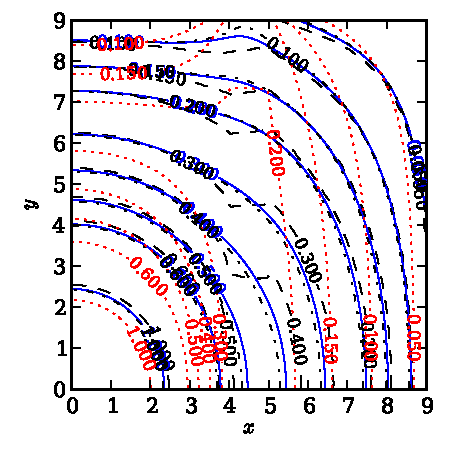
\includegraphics{ss_single_channel/phi.pdf}
  \Caption{ Contour plot of $\phi$ in the steady-state single channel problem.}{
  The dashed black line is the reference Monte Carlo solution; the dotted red
  line is standard diffusion; the broken black line is the anisotropic
  diffusion solution with analytic coefficients; the solid blue line is
  anisotropic diffusion with coefficients calculated with an S$_{32}$ transport
  sweep.}
  \label{fig:ssSingleContour}
\end{figure}

\begin{figure}[htb]
  \centering
  % GNUPLOT: LaTeX picture with Postscript
\begingroup
  \makeatletter
  \providecommand\color[2][]{%
    \GenericError{(gnuplot) \space\space\space\@spaces}{%
      Package color not loaded in conjunction with
      terminal option `colourtext'%
    }{See the gnuplot documentation for explanation.%
    }{Either use 'blacktext' in gnuplot or load the package
      color.sty in LaTeX.}%
    \renewcommand\color[2][]{}%
  }%
  \providecommand\includegraphics[2][]{%
    \GenericError{(gnuplot) \space\space\space\@spaces}{%
      Package graphicx or graphics not loaded%
    }{See the gnuplot documentation for explanation.%
    }{The gnuplot epslatex terminal needs graphicx.sty or graphics.sty.}%
    \renewcommand\includegraphics[2][]{}%
  }%
  \providecommand\rotatebox[2]{#2}%
  \@ifundefined{ifGPcolor}{%
    \newif\ifGPcolor
    \GPcolortrue
  }{}%
  \@ifundefined{ifGPblacktext}{%
    \newif\ifGPblacktext
    \GPblacktexttrue
  }{}%
  % define a \g@addto@macro without @ in the name:
  \let\gplgaddtomacro\g@addto@macro
  % define empty templates for all commands taking text:
  \gdef\gplbacktext{}%
  \gdef\gplfronttext{}%
  \makeatother
  \ifGPblacktext
    % no textcolor at all
    \def\colorrgb#1{}%
    \def\colorgray#1{}%
  \else
    % gray or color?
    \ifGPcolor
      \def\colorrgb#1{\color[rgb]{#1}}%
      \def\colorgray#1{\color[gray]{#1}}%
      \expandafter\def\csname LTw\endcsname{\color{white}}%
      \expandafter\def\csname LTb\endcsname{\color{black}}%
      \expandafter\def\csname LTa\endcsname{\color{black}}%
      \expandafter\def\csname LT0\endcsname{\color[rgb]{1,0,0}}%
      \expandafter\def\csname LT1\endcsname{\color[rgb]{0,1,0}}%
      \expandafter\def\csname LT2\endcsname{\color[rgb]{0,0,1}}%
      \expandafter\def\csname LT3\endcsname{\color[rgb]{1,0,1}}%
      \expandafter\def\csname LT4\endcsname{\color[rgb]{0,1,1}}%
      \expandafter\def\csname LT5\endcsname{\color[rgb]{1,1,0}}%
      \expandafter\def\csname LT6\endcsname{\color[rgb]{0,0,0}}%
      \expandafter\def\csname LT7\endcsname{\color[rgb]{1,0.3,0}}%
      \expandafter\def\csname LT8\endcsname{\color[rgb]{0.5,0.5,0.5}}%
    \else
      % gray
      \def\colorrgb#1{\color{black}}%
      \def\colorgray#1{\color[gray]{#1}}%
      \expandafter\def\csname LTw\endcsname{\color{white}}%
      \expandafter\def\csname LTb\endcsname{\color{black}}%
      \expandafter\def\csname LTa\endcsname{\color{black}}%
      \expandafter\def\csname LT0\endcsname{\color{black}}%
      \expandafter\def\csname LT1\endcsname{\color{black}}%
      \expandafter\def\csname LT2\endcsname{\color{black}}%
      \expandafter\def\csname LT3\endcsname{\color{black}}%
      \expandafter\def\csname LT4\endcsname{\color{black}}%
      \expandafter\def\csname LT5\endcsname{\color{black}}%
      \expandafter\def\csname LT6\endcsname{\color{black}}%
      \expandafter\def\csname LT7\endcsname{\color{black}}%
      \expandafter\def\csname LT8\endcsname{\color{black}}%
    \fi
  \fi
  \setlength{\unitlength}{0.0500bp}%
  \begin{picture}(7200.00,4320.00)%
    \gplgaddtomacro\gplbacktext{%
      \csname LTb\endcsname%
      \put(1910,400){\makebox(0,0)[r]{\strut{} 0.1}}%
      \put(1910,768){\makebox(0,0)[r]{\strut{} 0.08}}%
      \put(1910,1136){\makebox(0,0)[r]{\strut{} 0.06}}%
      \put(1910,1504){\makebox(0,0)[r]{\strut{} 0.04}}%
      \put(1910,1872){\makebox(0,0)[r]{\strut{} 0.02}}%
      \put(1910,2240){\makebox(0,0)[r]{\strut{} 0}}%
      \put(1910,2607){\makebox(0,0)[r]{\strut{} 0.02}}%
      \put(1910,2975){\makebox(0,0)[r]{\strut{} 0.04}}%
      \put(1910,3343){\makebox(0,0)[r]{\strut{} 0.06}}%
      \put(1910,3711){\makebox(0,0)[r]{\strut{} 0.08}}%
      \put(1910,4079){\makebox(0,0)[r]{\strut{} 0.1}}%
      \csname LTb\endcsname%
      \put(2030,200){\makebox(0,0){\strut{} 0.02}}%
      \csname LTb\endcsname%
      \put(2364,200){\makebox(0,0){\strut{} 0}}%
      \csname LTb\endcsname%
      \put(2699,200){\makebox(0,0){\strut{} 0.02}}%
      \csname LTb\endcsname%
      \put(3033,200){\makebox(0,0){\strut{} 0.04}}%
      \csname LTb\endcsname%
      \put(3368,200){\makebox(0,0){\strut{} 0.06}}%
      \csname LTb\endcsname%
      \put(3702,200){\makebox(0,0){\strut{} 0.08}}%
      \csname LTb\endcsname%
      \put(4037,200){\makebox(0,0){\strut{} 0.1}}%
      \csname LTb\endcsname%
      \put(4371,200){\makebox(0,0){\strut{} 0.12}}%
      \csname LTb\endcsname%
      \put(4706,200){\makebox(0,0){\strut{} 0.14}}%
      \csname LTb\endcsname%
      \put(5040,200){\makebox(0,0){\strut{} 0.16}}%
      \csname LTb\endcsname%
      \put(5375,200){\makebox(0,0){\strut{} 0.18}}%
      \csname LTb\endcsname%
      \put(5709,200){\makebox(0,0){\strut{} 0.2}}%
      \csname LTb\endcsname%
      \put(1330,2239){\rotatebox{-270}{\makebox(0,0){\strut{}x1 center $(1.01,3.5)$}}}%
    }%
    \gplgaddtomacro\gplfronttext{%
      \csname LTb\endcsname%
      \put(4806,3916){\makebox(0,0)[r]{\strut{}S$_{128}$}}%
      \csname LTb\endcsname%
      \put(4806,3716){\makebox(0,0)[r]{\strut{}FLAD$_{64}$}}%
      \csname LTb\endcsname%
      \put(4806,3516){\makebox(0,0)[r]{\strut{}AD$_{64}$}}%
      \csname LTb\endcsname%
      \put(4806,3316){\makebox(0,0)[r]{\strut{}FLD}}%
    }%
    \gplbacktext
    \put(0,0){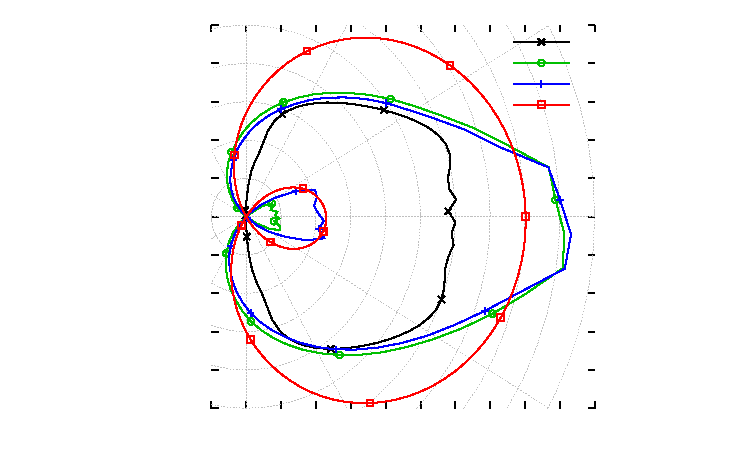
\includegraphics{/Users/seth/_thesis/figures/crashpipe2b/intens-x1-t1/intensity-x1-t1.pdf}}%
    \gplfronttext
  \end{picture}%
\endgroup

  \Caption{Scalar intensity along $x=5.0$.}{
    The ``AD'' curve is the solution using analytic diffusion coefficients;
  the ``AD$_N$'' curves use S$_N$-calculated coefficients.}
  \label{fig:ssSingleCenterline}
\end{figure}

\subsection{\texorpdfstring{\SN}{SN} parameter convergence}
Figure~\ref{fig:ssSingleAbsConv} plots the convergence of the solution $\phi$
against the solution with analytically-calculated AD coefficients, for four
different combinations of \SN\ solver parameters, as a function of the number of
source iterations (transport sweeps) in the calculation of $f$.

Likewise, figure~\ref{fig:ssSingleQsConv} plots the convergence of the \SN\ 
solution with increasing number of ordinates. The black line shows that refining
the quadrature brings the solution closer to the analytic value, but the red
line demonstrates that it does \emph{not} converge to the Monte Carlo transport
solution. This is expected: anisotropic diffusion contains several
approximations that are small but not zero in this problem. As with diffusion,
we run problems far outside their theoretical (asymptotic) range of
applicability: the true solution is strongly anisotropic and has strong
gradients at the channel interface.
Unlike diffusion, anisotropic diffusion yields reasonable answers in the
presence of voids.

\begin{figure}[htb]
  \centering
  \subfloat[Source iterations]{%
    \label{fig:ssSingleAbsConv}
    % GNUPLOT: LaTeX picture with Postscript
\begingroup
  \makeatletter
  \providecommand\color[2][]{%
    \GenericError{(gnuplot) \space\space\space\@spaces}{%
      Package color not loaded in conjunction with
      terminal option `colourtext'%
    }{See the gnuplot documentation for explanation.%
    }{Either use 'blacktext' in gnuplot or load the package
      color.sty in LaTeX.}%
    \renewcommand\color[2][]{}%
  }%
  \providecommand\includegraphics[2][]{%
    \GenericError{(gnuplot) \space\space\space\@spaces}{%
      Package graphicx or graphics not loaded%
    }{See the gnuplot documentation for explanation.%
    }{The gnuplot epslatex terminal needs graphicx.sty or graphics.sty.}%
    \renewcommand\includegraphics[2][]{}%
  }%
  \providecommand\rotatebox[2]{#2}%
  \@ifundefined{ifGPcolor}{%
    \newif\ifGPcolor
    \GPcolortrue
  }{}%
  \@ifundefined{ifGPblacktext}{%
    \newif\ifGPblacktext
    \GPblacktexttrue
  }{}%
  % define a \g@addto@macro without @ in the name:
  \let\gplgaddtomacro\g@addto@macro
  % define empty templates for all commands taking text:
  \gdef\gplbacktext{}%
  \gdef\gplfronttext{}%
  \makeatother
  \ifGPblacktext
    % no textcolor at all
    \def\colorrgb#1{}%
    \def\colorgray#1{}%
  \else
    % gray or color?
    \ifGPcolor
      \def\colorrgb#1{\color[rgb]{#1}}%
      \def\colorgray#1{\color[gray]{#1}}%
      \expandafter\def\csname LTw\endcsname{\color{white}}%
      \expandafter\def\csname LTb\endcsname{\color{black}}%
      \expandafter\def\csname LTa\endcsname{\color{black}}%
      \expandafter\def\csname LT0\endcsname{\color[rgb]{1,0,0}}%
      \expandafter\def\csname LT1\endcsname{\color[rgb]{0,1,0}}%
      \expandafter\def\csname LT2\endcsname{\color[rgb]{0,0,1}}%
      \expandafter\def\csname LT3\endcsname{\color[rgb]{1,0,1}}%
      \expandafter\def\csname LT4\endcsname{\color[rgb]{0,1,1}}%
      \expandafter\def\csname LT5\endcsname{\color[rgb]{1,1,0}}%
      \expandafter\def\csname LT6\endcsname{\color[rgb]{0,0,0}}%
      \expandafter\def\csname LT7\endcsname{\color[rgb]{1,0.3,0}}%
      \expandafter\def\csname LT8\endcsname{\color[rgb]{0.5,0.5,0.5}}%
    \else
      % gray
      \def\colorrgb#1{\color{black}}%
      \def\colorgray#1{\color[gray]{#1}}%
      \expandafter\def\csname LTw\endcsname{\color{white}}%
      \expandafter\def\csname LTb\endcsname{\color{black}}%
      \expandafter\def\csname LTa\endcsname{\color{black}}%
      \expandafter\def\csname LT0\endcsname{\color{black}}%
      \expandafter\def\csname LT1\endcsname{\color{black}}%
      \expandafter\def\csname LT2\endcsname{\color{black}}%
      \expandafter\def\csname LT3\endcsname{\color{black}}%
      \expandafter\def\csname LT4\endcsname{\color{black}}%
      \expandafter\def\csname LT5\endcsname{\color{black}}%
      \expandafter\def\csname LT6\endcsname{\color{black}}%
      \expandafter\def\csname LT7\endcsname{\color{black}}%
      \expandafter\def\csname LT8\endcsname{\color{black}}%
    \fi
  \fi
  \setlength{\unitlength}{0.0500bp}%
  \begin{picture}(7200.00,4320.00)%
    \gplgaddtomacro\gplbacktext{%
      \csname LTb\endcsname%
      \put(1910,400){\makebox(0,0)[r]{\strut{} 0.1}}%
      \put(1910,768){\makebox(0,0)[r]{\strut{} 0.08}}%
      \put(1910,1136){\makebox(0,0)[r]{\strut{} 0.06}}%
      \put(1910,1504){\makebox(0,0)[r]{\strut{} 0.04}}%
      \put(1910,1872){\makebox(0,0)[r]{\strut{} 0.02}}%
      \put(1910,2240){\makebox(0,0)[r]{\strut{} 0}}%
      \put(1910,2607){\makebox(0,0)[r]{\strut{} 0.02}}%
      \put(1910,2975){\makebox(0,0)[r]{\strut{} 0.04}}%
      \put(1910,3343){\makebox(0,0)[r]{\strut{} 0.06}}%
      \put(1910,3711){\makebox(0,0)[r]{\strut{} 0.08}}%
      \put(1910,4079){\makebox(0,0)[r]{\strut{} 0.1}}%
      \csname LTb\endcsname%
      \put(2030,200){\makebox(0,0){\strut{} 0.02}}%
      \csname LTb\endcsname%
      \put(2364,200){\makebox(0,0){\strut{} 0}}%
      \csname LTb\endcsname%
      \put(2699,200){\makebox(0,0){\strut{} 0.02}}%
      \csname LTb\endcsname%
      \put(3033,200){\makebox(0,0){\strut{} 0.04}}%
      \csname LTb\endcsname%
      \put(3368,200){\makebox(0,0){\strut{} 0.06}}%
      \csname LTb\endcsname%
      \put(3702,200){\makebox(0,0){\strut{} 0.08}}%
      \csname LTb\endcsname%
      \put(4037,200){\makebox(0,0){\strut{} 0.1}}%
      \csname LTb\endcsname%
      \put(4371,200){\makebox(0,0){\strut{} 0.12}}%
      \csname LTb\endcsname%
      \put(4706,200){\makebox(0,0){\strut{} 0.14}}%
      \csname LTb\endcsname%
      \put(5040,200){\makebox(0,0){\strut{} 0.16}}%
      \csname LTb\endcsname%
      \put(5375,200){\makebox(0,0){\strut{} 0.18}}%
      \csname LTb\endcsname%
      \put(5709,200){\makebox(0,0){\strut{} 0.2}}%
      \csname LTb\endcsname%
      \put(1330,2239){\rotatebox{-270}{\makebox(0,0){\strut{}x1 center $(1.01,3.5)$}}}%
    }%
    \gplgaddtomacro\gplfronttext{%
      \csname LTb\endcsname%
      \put(4806,3916){\makebox(0,0)[r]{\strut{}S$_{128}$}}%
      \csname LTb\endcsname%
      \put(4806,3716){\makebox(0,0)[r]{\strut{}FLAD$_{64}$}}%
      \csname LTb\endcsname%
      \put(4806,3516){\makebox(0,0)[r]{\strut{}AD$_{64}$}}%
      \csname LTb\endcsname%
      \put(4806,3316){\makebox(0,0)[r]{\strut{}FLD}}%
    }%
    \gplbacktext
    \put(0,0){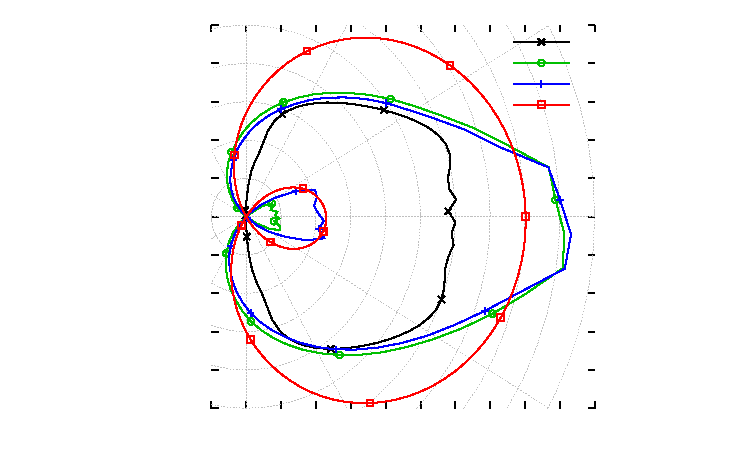
\includegraphics{/Users/seth/_thesis/figures/crashpipe2b/intens-x1-t1/intensity-x1-t1.pdf}}%
    \gplfronttext
  \end{picture}%
\endgroup
}%
  \subfloat[Quadrature sets]{%
    \label{fig:ssSingleQsConv}
    % GNUPLOT: LaTeX picture with Postscript
\begingroup
  \makeatletter
  \providecommand\color[2][]{%
    \GenericError{(gnuplot) \space\space\space\@spaces}{%
      Package color not loaded in conjunction with
      terminal option `colourtext'%
    }{See the gnuplot documentation for explanation.%
    }{Either use 'blacktext' in gnuplot or load the package
      color.sty in LaTeX.}%
    \renewcommand\color[2][]{}%
  }%
  \providecommand\includegraphics[2][]{%
    \GenericError{(gnuplot) \space\space\space\@spaces}{%
      Package graphicx or graphics not loaded%
    }{See the gnuplot documentation for explanation.%
    }{The gnuplot epslatex terminal needs graphicx.sty or graphics.sty.}%
    \renewcommand\includegraphics[2][]{}%
  }%
  \providecommand\rotatebox[2]{#2}%
  \@ifundefined{ifGPcolor}{%
    \newif\ifGPcolor
    \GPcolortrue
  }{}%
  \@ifundefined{ifGPblacktext}{%
    \newif\ifGPblacktext
    \GPblacktexttrue
  }{}%
  % define a \g@addto@macro without @ in the name:
  \let\gplgaddtomacro\g@addto@macro
  % define empty templates for all commands taking text:
  \gdef\gplbacktext{}%
  \gdef\gplfronttext{}%
  \makeatother
  \ifGPblacktext
    % no textcolor at all
    \def\colorrgb#1{}%
    \def\colorgray#1{}%
  \else
    % gray or color?
    \ifGPcolor
      \def\colorrgb#1{\color[rgb]{#1}}%
      \def\colorgray#1{\color[gray]{#1}}%
      \expandafter\def\csname LTw\endcsname{\color{white}}%
      \expandafter\def\csname LTb\endcsname{\color{black}}%
      \expandafter\def\csname LTa\endcsname{\color{black}}%
      \expandafter\def\csname LT0\endcsname{\color[rgb]{1,0,0}}%
      \expandafter\def\csname LT1\endcsname{\color[rgb]{0,1,0}}%
      \expandafter\def\csname LT2\endcsname{\color[rgb]{0,0,1}}%
      \expandafter\def\csname LT3\endcsname{\color[rgb]{1,0,1}}%
      \expandafter\def\csname LT4\endcsname{\color[rgb]{0,1,1}}%
      \expandafter\def\csname LT5\endcsname{\color[rgb]{1,1,0}}%
      \expandafter\def\csname LT6\endcsname{\color[rgb]{0,0,0}}%
      \expandafter\def\csname LT7\endcsname{\color[rgb]{1,0.3,0}}%
      \expandafter\def\csname LT8\endcsname{\color[rgb]{0.5,0.5,0.5}}%
    \else
      % gray
      \def\colorrgb#1{\color{black}}%
      \def\colorgray#1{\color[gray]{#1}}%
      \expandafter\def\csname LTw\endcsname{\color{white}}%
      \expandafter\def\csname LTb\endcsname{\color{black}}%
      \expandafter\def\csname LTa\endcsname{\color{black}}%
      \expandafter\def\csname LT0\endcsname{\color{black}}%
      \expandafter\def\csname LT1\endcsname{\color{black}}%
      \expandafter\def\csname LT2\endcsname{\color{black}}%
      \expandafter\def\csname LT3\endcsname{\color{black}}%
      \expandafter\def\csname LT4\endcsname{\color{black}}%
      \expandafter\def\csname LT5\endcsname{\color{black}}%
      \expandafter\def\csname LT6\endcsname{\color{black}}%
      \expandafter\def\csname LT7\endcsname{\color{black}}%
      \expandafter\def\csname LT8\endcsname{\color{black}}%
    \fi
  \fi
  \setlength{\unitlength}{0.0500bp}%
  \begin{picture}(7200.00,4320.00)%
    \gplgaddtomacro\gplbacktext{%
      \csname LTb\endcsname%
      \put(1910,400){\makebox(0,0)[r]{\strut{} 0.1}}%
      \put(1910,768){\makebox(0,0)[r]{\strut{} 0.08}}%
      \put(1910,1136){\makebox(0,0)[r]{\strut{} 0.06}}%
      \put(1910,1504){\makebox(0,0)[r]{\strut{} 0.04}}%
      \put(1910,1872){\makebox(0,0)[r]{\strut{} 0.02}}%
      \put(1910,2240){\makebox(0,0)[r]{\strut{} 0}}%
      \put(1910,2607){\makebox(0,0)[r]{\strut{} 0.02}}%
      \put(1910,2975){\makebox(0,0)[r]{\strut{} 0.04}}%
      \put(1910,3343){\makebox(0,0)[r]{\strut{} 0.06}}%
      \put(1910,3711){\makebox(0,0)[r]{\strut{} 0.08}}%
      \put(1910,4079){\makebox(0,0)[r]{\strut{} 0.1}}%
      \csname LTb\endcsname%
      \put(2030,200){\makebox(0,0){\strut{} 0.02}}%
      \csname LTb\endcsname%
      \put(2364,200){\makebox(0,0){\strut{} 0}}%
      \csname LTb\endcsname%
      \put(2699,200){\makebox(0,0){\strut{} 0.02}}%
      \csname LTb\endcsname%
      \put(3033,200){\makebox(0,0){\strut{} 0.04}}%
      \csname LTb\endcsname%
      \put(3368,200){\makebox(0,0){\strut{} 0.06}}%
      \csname LTb\endcsname%
      \put(3702,200){\makebox(0,0){\strut{} 0.08}}%
      \csname LTb\endcsname%
      \put(4037,200){\makebox(0,0){\strut{} 0.1}}%
      \csname LTb\endcsname%
      \put(4371,200){\makebox(0,0){\strut{} 0.12}}%
      \csname LTb\endcsname%
      \put(4706,200){\makebox(0,0){\strut{} 0.14}}%
      \csname LTb\endcsname%
      \put(5040,200){\makebox(0,0){\strut{} 0.16}}%
      \csname LTb\endcsname%
      \put(5375,200){\makebox(0,0){\strut{} 0.18}}%
      \csname LTb\endcsname%
      \put(5709,200){\makebox(0,0){\strut{} 0.2}}%
      \csname LTb\endcsname%
      \put(1330,2239){\rotatebox{-270}{\makebox(0,0){\strut{}x1 center $(1.01,3.5)$}}}%
    }%
    \gplgaddtomacro\gplfronttext{%
      \csname LTb\endcsname%
      \put(4806,3916){\makebox(0,0)[r]{\strut{}S$_{128}$}}%
      \csname LTb\endcsname%
      \put(4806,3716){\makebox(0,0)[r]{\strut{}FLAD$_{64}$}}%
      \csname LTb\endcsname%
      \put(4806,3516){\makebox(0,0)[r]{\strut{}AD$_{64}$}}%
      \csname LTb\endcsname%
      \put(4806,3316){\makebox(0,0)[r]{\strut{}FLD}}%
    }%
    \gplbacktext
    \put(0,0){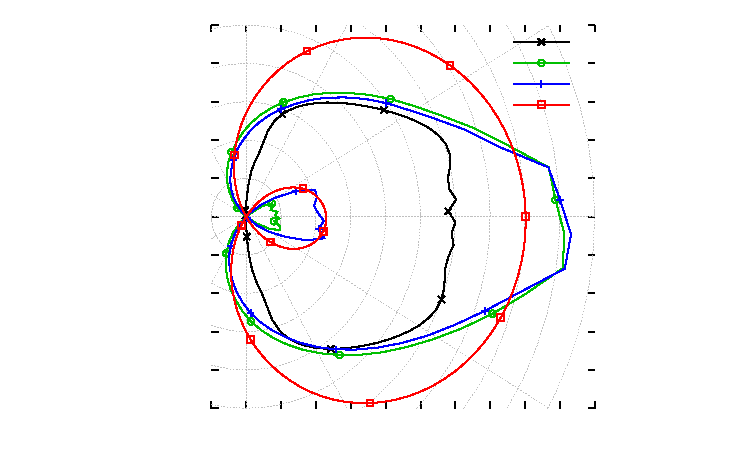
\includegraphics{/Users/seth/_thesis/figures/crashpipe2b/intens-x1-t1/intensity-x1-t1.pdf}}%
    \gplfronttext
  \end{picture}%
\endgroup
}%
  \Caption{Convergence of $\phi$ as a function of \SN\ parameters.}{
    The AD solution $\phi$ with \SN-calculated coefficients is compared
    against the solution with analytic coefficients using a volume-weighted
    2-norm, as a function of increasing source iterations in the calculation of
    $f$. The red line in (b) shows convergence compared to the Monte Carlo
    solution.}
  \label{fig:ssSingleConv}
\end{figure}

The convergence is calculated using a volume-weighted relative 2-norm:
\begin{equation}\label{eq:rel2norm}
  \text{reported difference} =
  \left[ \sum_{i \in \text{cells}} \left(
  \frac{\phi_i}{\phi_{i,\text{reference}}} - 1 \right)^2 (V_i)^2\right]^{1/2} \,.
\end{equation}
This is \emph{not} the convergence of the transport solution $f$, which only
indirectly affects the $\phi$.
Compared to the reference solution, AD (with analytic coefficients) has a 4.5\%
absolute error and standard diffusion has a 19.8\% error.

The data in Fig.~\ref{fig:ssSingleAbsConv} suggest that with a finite number of
ordinates, which cannot exactly
approximate the angular domain, there is little added benefit to using more than
a few sweeps: the error introduced by the angular approximation exceeds that
caused by 
the lack of convergence. But Fig.~\ref{fig:ssSingleQsConv} shows that, since
the analytic AD solution differs from the exact solution by ~5\%, even a
coarse quadrature set can provide accuracy within the inherent limits of the
method.
%Additionally, the choice of reflecting or white boundary conditions has
%little effect on the solution of this problem.

This conclusion may not hold for all problems, of course, but it suggests that
a modest number of ordinates and sweeps are sufficient to yield solutions with
close to the accuracy of an analytic anisotropic diffusion solution.

\subsection{Coarse spatial grid calculation of \texorpdfstring{$\Dtens$}{D}}
\label{sec:coarseGridAdCoeff}

In addition to investigating the sensitivity of the AD solution to the
granularity of
the angular variable in the solution of $f$, we test the discrepancy
introduced by calculating $f$ on a coarser spatial grid. As discussed in
\S\ref{sec:adSmoothness}, the function $f$ is a smooth function of space, and
$\Dtens$ likewise has no discontinuities. We have implemented the basic
multigrid operations of prolongation and restriction in the \pytrt\ code
for cell-centered quantities and quantities on the boundary face \cite{Pytrt}.

%The total opacity is restricted using a volume-weighted harmonic average 
We run the transport calculation for $f$ on a coarse grid and prolongate the
diffusion tensor $\Dtens$ and boundary coefficient $\vec{d}$ back to the fine
grid, in which $\phi$
is then solved. With this methodology, the spatial discretization error of the
diffusion solve is unaffected; the only difference is that the diffusion
coefficients are coarser functions of space. Figure~\ref{fig:ssSingleMgD} shows
the resulting coarse anisotropic diffusion coefficients.

\begin{figure}[htb]
  \centering
\subfloat[$D^{xx}$]{%
  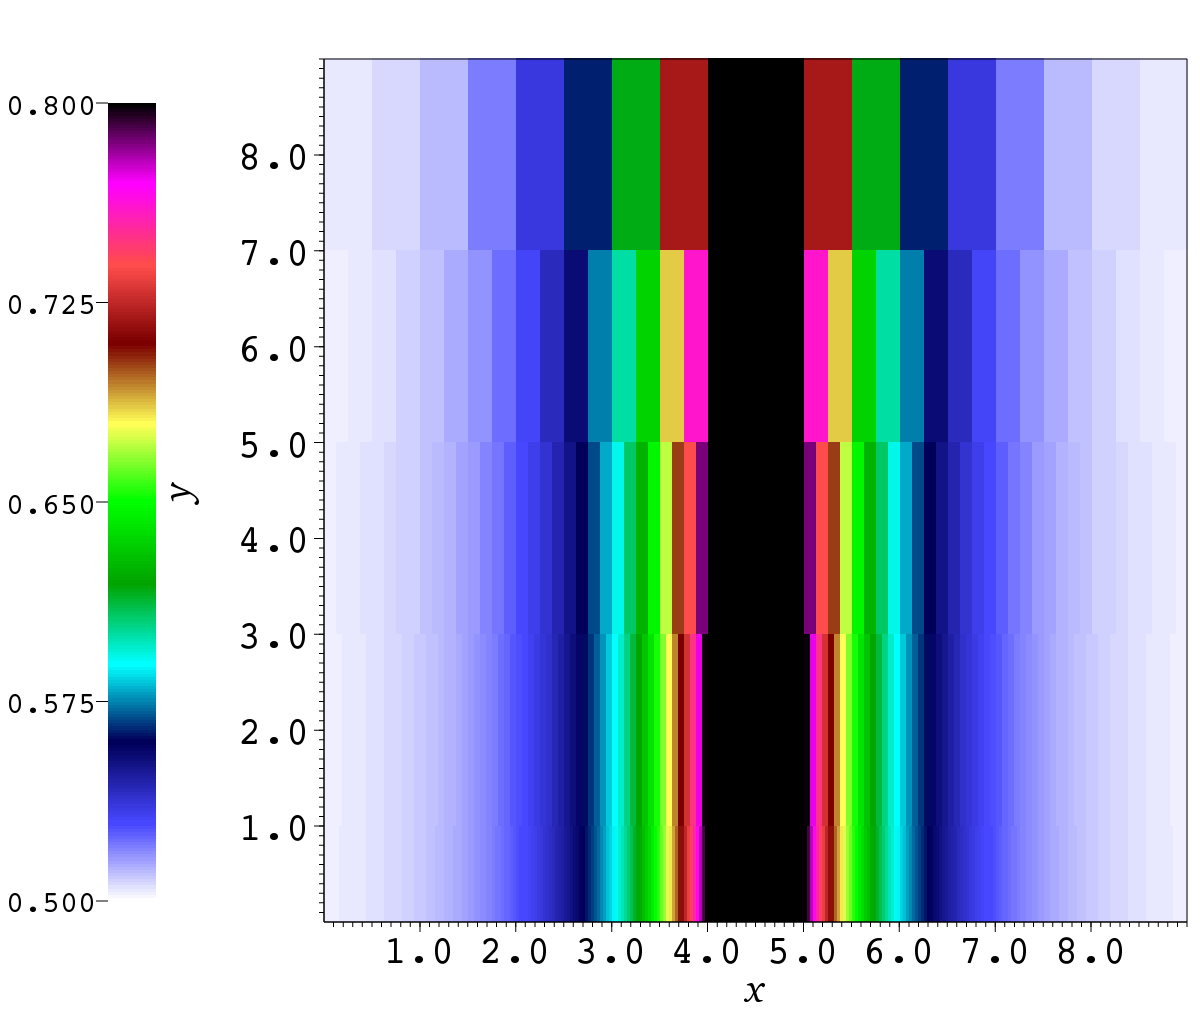
\includegraphics[width=3in]{ss_single_channel/mg-dxx.png}}%
\subfloat[$D^{yy}$]{%
  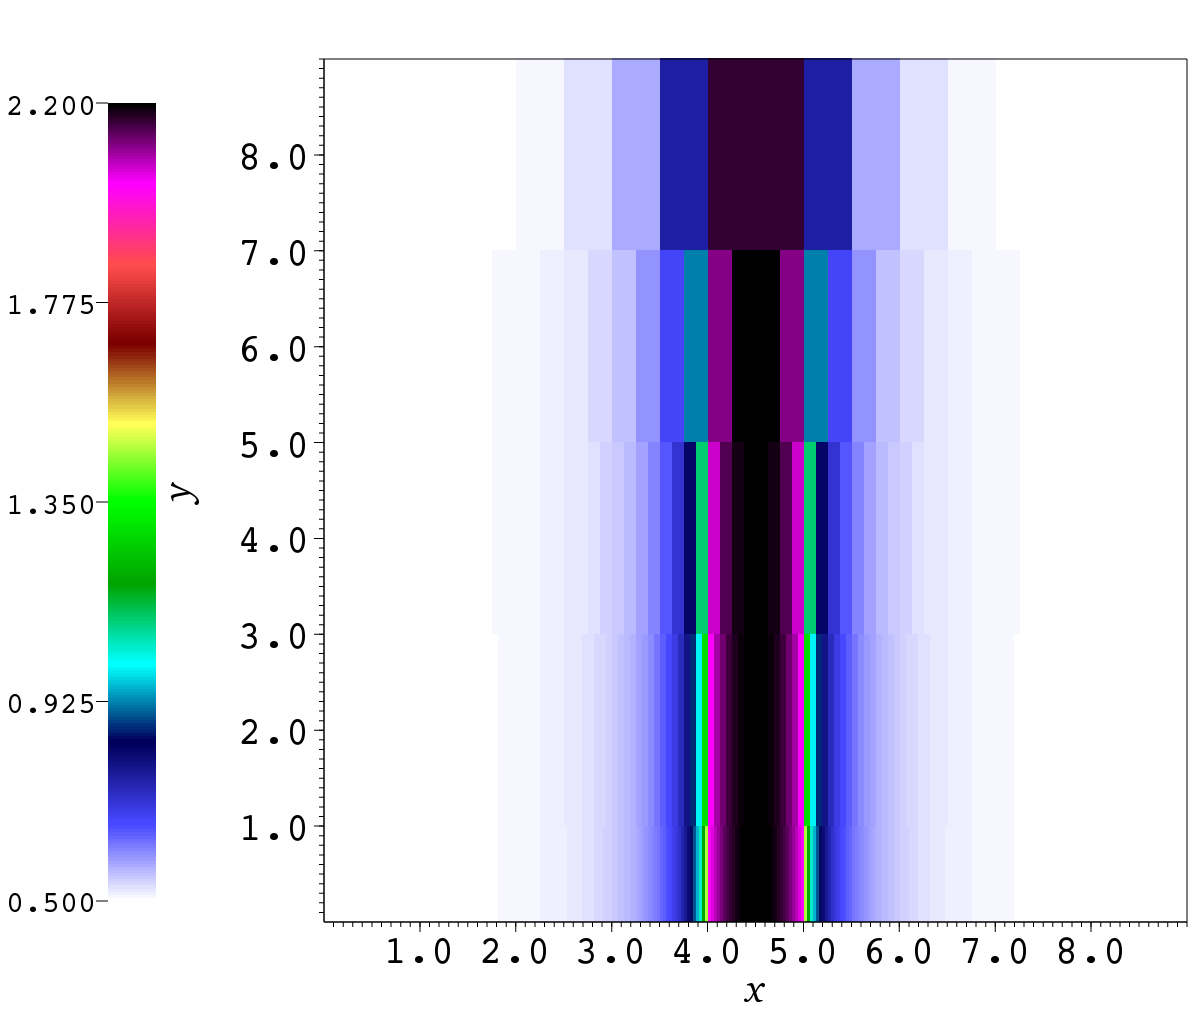
\includegraphics[width=3in]{ss_single_channel/mg-dyy.png}}%
  \Caption{Calculated diffusion coefficients for different grid coarseness.}{
  Every two units downward represents a factor of four refinement in the
  number of fine cells per coarse cell.}
  \label{fig:ssSingleMgD}
\end{figure}

Figure~\ref{fig:ssSingleMgConv} plots the error in $\phi$ introduced by using
%
\begin{figure}[htb]
  \centering
  % GNUPLOT: LaTeX picture with Postscript
\begingroup
  \makeatletter
  \providecommand\color[2][]{%
    \GenericError{(gnuplot) \space\space\space\@spaces}{%
      Package color not loaded in conjunction with
      terminal option `colourtext'%
    }{See the gnuplot documentation for explanation.%
    }{Either use 'blacktext' in gnuplot or load the package
      color.sty in LaTeX.}%
    \renewcommand\color[2][]{}%
  }%
  \providecommand\includegraphics[2][]{%
    \GenericError{(gnuplot) \space\space\space\@spaces}{%
      Package graphicx or graphics not loaded%
    }{See the gnuplot documentation for explanation.%
    }{The gnuplot epslatex terminal needs graphicx.sty or graphics.sty.}%
    \renewcommand\includegraphics[2][]{}%
  }%
  \providecommand\rotatebox[2]{#2}%
  \@ifundefined{ifGPcolor}{%
    \newif\ifGPcolor
    \GPcolortrue
  }{}%
  \@ifundefined{ifGPblacktext}{%
    \newif\ifGPblacktext
    \GPblacktexttrue
  }{}%
  % define a \g@addto@macro without @ in the name:
  \let\gplgaddtomacro\g@addto@macro
  % define empty templates for all commands taking text:
  \gdef\gplbacktext{}%
  \gdef\gplfronttext{}%
  \makeatother
  \ifGPblacktext
    % no textcolor at all
    \def\colorrgb#1{}%
    \def\colorgray#1{}%
  \else
    % gray or color?
    \ifGPcolor
      \def\colorrgb#1{\color[rgb]{#1}}%
      \def\colorgray#1{\color[gray]{#1}}%
      \expandafter\def\csname LTw\endcsname{\color{white}}%
      \expandafter\def\csname LTb\endcsname{\color{black}}%
      \expandafter\def\csname LTa\endcsname{\color{black}}%
      \expandafter\def\csname LT0\endcsname{\color[rgb]{1,0,0}}%
      \expandafter\def\csname LT1\endcsname{\color[rgb]{0,1,0}}%
      \expandafter\def\csname LT2\endcsname{\color[rgb]{0,0,1}}%
      \expandafter\def\csname LT3\endcsname{\color[rgb]{1,0,1}}%
      \expandafter\def\csname LT4\endcsname{\color[rgb]{0,1,1}}%
      \expandafter\def\csname LT5\endcsname{\color[rgb]{1,1,0}}%
      \expandafter\def\csname LT6\endcsname{\color[rgb]{0,0,0}}%
      \expandafter\def\csname LT7\endcsname{\color[rgb]{1,0.3,0}}%
      \expandafter\def\csname LT8\endcsname{\color[rgb]{0.5,0.5,0.5}}%
    \else
      % gray
      \def\colorrgb#1{\color{black}}%
      \def\colorgray#1{\color[gray]{#1}}%
      \expandafter\def\csname LTw\endcsname{\color{white}}%
      \expandafter\def\csname LTb\endcsname{\color{black}}%
      \expandafter\def\csname LTa\endcsname{\color{black}}%
      \expandafter\def\csname LT0\endcsname{\color{black}}%
      \expandafter\def\csname LT1\endcsname{\color{black}}%
      \expandafter\def\csname LT2\endcsname{\color{black}}%
      \expandafter\def\csname LT3\endcsname{\color{black}}%
      \expandafter\def\csname LT4\endcsname{\color{black}}%
      \expandafter\def\csname LT5\endcsname{\color{black}}%
      \expandafter\def\csname LT6\endcsname{\color{black}}%
      \expandafter\def\csname LT7\endcsname{\color{black}}%
      \expandafter\def\csname LT8\endcsname{\color{black}}%
    \fi
  \fi
  \setlength{\unitlength}{0.0500bp}%
  \begin{picture}(7200.00,4320.00)%
    \gplgaddtomacro\gplbacktext{%
      \csname LTb\endcsname%
      \put(1910,400){\makebox(0,0)[r]{\strut{} 0.1}}%
      \put(1910,768){\makebox(0,0)[r]{\strut{} 0.08}}%
      \put(1910,1136){\makebox(0,0)[r]{\strut{} 0.06}}%
      \put(1910,1504){\makebox(0,0)[r]{\strut{} 0.04}}%
      \put(1910,1872){\makebox(0,0)[r]{\strut{} 0.02}}%
      \put(1910,2240){\makebox(0,0)[r]{\strut{} 0}}%
      \put(1910,2607){\makebox(0,0)[r]{\strut{} 0.02}}%
      \put(1910,2975){\makebox(0,0)[r]{\strut{} 0.04}}%
      \put(1910,3343){\makebox(0,0)[r]{\strut{} 0.06}}%
      \put(1910,3711){\makebox(0,0)[r]{\strut{} 0.08}}%
      \put(1910,4079){\makebox(0,0)[r]{\strut{} 0.1}}%
      \csname LTb\endcsname%
      \put(2030,200){\makebox(0,0){\strut{} 0.02}}%
      \csname LTb\endcsname%
      \put(2364,200){\makebox(0,0){\strut{} 0}}%
      \csname LTb\endcsname%
      \put(2699,200){\makebox(0,0){\strut{} 0.02}}%
      \csname LTb\endcsname%
      \put(3033,200){\makebox(0,0){\strut{} 0.04}}%
      \csname LTb\endcsname%
      \put(3368,200){\makebox(0,0){\strut{} 0.06}}%
      \csname LTb\endcsname%
      \put(3702,200){\makebox(0,0){\strut{} 0.08}}%
      \csname LTb\endcsname%
      \put(4037,200){\makebox(0,0){\strut{} 0.1}}%
      \csname LTb\endcsname%
      \put(4371,200){\makebox(0,0){\strut{} 0.12}}%
      \csname LTb\endcsname%
      \put(4706,200){\makebox(0,0){\strut{} 0.14}}%
      \csname LTb\endcsname%
      \put(5040,200){\makebox(0,0){\strut{} 0.16}}%
      \csname LTb\endcsname%
      \put(5375,200){\makebox(0,0){\strut{} 0.18}}%
      \csname LTb\endcsname%
      \put(5709,200){\makebox(0,0){\strut{} 0.2}}%
      \csname LTb\endcsname%
      \put(1330,2239){\rotatebox{-270}{\makebox(0,0){\strut{}x1 center $(1.01,3.5)$}}}%
    }%
    \gplgaddtomacro\gplfronttext{%
      \csname LTb\endcsname%
      \put(4806,3916){\makebox(0,0)[r]{\strut{}S$_{128}$}}%
      \csname LTb\endcsname%
      \put(4806,3716){\makebox(0,0)[r]{\strut{}FLAD$_{64}$}}%
      \csname LTb\endcsname%
      \put(4806,3516){\makebox(0,0)[r]{\strut{}AD$_{64}$}}%
      \csname LTb\endcsname%
      \put(4806,3316){\makebox(0,0)[r]{\strut{}FLD}}%
    }%
    \gplbacktext
    \put(0,0){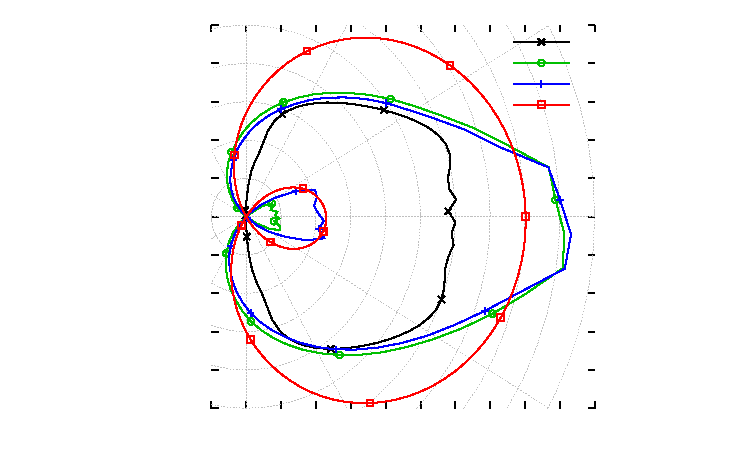
\includegraphics{/Users/seth/_thesis/figures/crashpipe2b/intens-x1-t1/intensity-x1-t1.pdf}}%
    \gplfronttext
  \end{picture}%
\endgroup

  \caption{Error introduced by coarse spatial grids in calculating the AD
  coefficients.}
  \label{fig:ssSingleMgConv}
\end{figure}
%
coarse approximations to the anisotropic diffusion coefficient. (In this
problem, the grid and refinements were chosen so that in the coarsest case, each
coarse cell was composed of a single material.) 
The rightmost data point in the figure has a coarse cell width of
$\Delta_x=0.5$, half the width of the channel.
In this simple problem with well-defined material boundaries, the
solution is relatively insensitive to using less spatially refined diffusion
coefficients. This is perhaps not surprising, as, for example, the standard
diffusion coefficient has no spatial variation inside a homogeneous material.

The implication of all these results is clear: high-fidelity transport
calculations are \emph{not} needed in calculation of the anisotropic diffusion
coefficients. Because the cost of the transport calculation is
roughly proportional to $
  (\text{the number of transport sweeps}) \times 
  (\text{the number of ordinates}) \times 
  (\text{the number of spatial cells})$,
using only a modest number of sweeps and a small quadrature set with a
coarse-grid calculation can provide a substantial speedup when compared with a
fine-grid calculation that might improve the answer only by a tenth of a
percent. Because we do not expect the anisotropic diffusion approximation to
yield exact transport solutions, and because a high-fidelity transport
calculation requires far more computational effort than a diffusion solve, the
small error incurred by using a coarse transport solution is justifiable in
light of the performance gain.

%%%%%%%%%%%%%%%%%%%%%%%%%%%%%%%%%%%%%%%%%%%%%%%%%%%%%%%%%%%%%%%%%%%%%%%%%%%%%%%%
\section{Flatland boundary conditions}\label{sec:nrFlatlandBcs}

The flatland boundary conditions derived in Chapter~\ref{chap:flatland} must,
for the sake of completeness, be numerically verified. We compare the novel
diffusion boundary conditions against a Monte Carlo reference solution in a
simple, diffusive test problem.

We consider a homogeneous flatland problem (Fig.~\ref{fig:flatlandBcProblem})
with a
total cross section $\sigma=1$ and scattering ratio $c=0.99$. The spatial 
domain is the rectangle $0 \le x \le 2$, $0 \le y \le 10$, with
reflecting boundaries on the left,
right, and top sides. The bottom side has a specified unit incident radiation
flux; we consider three different angular
distributions given in Table~\ref{tab:angularDistributions}.\footnote{These
distributions were chosen because of their prior use in a 1-D boundary
matching analysis in Ref.~\cite{Dav2006}.}

\begin{figure}[htb]
  \centering
  \includegraphics[width=4in]{flatlandbc-problem}
  \caption{Problem description for the flatland boundary test.}
  \label{fig:flatlandBcProblem}
\end{figure}

\begin{table}[htb]
  \centering
  \begin{tabular}{ccc}
\toprule
    Distribution & 1-D & Flatland
\\ \midrule
Isotropic & $I(\mu) = \frac{1}{2}$ & $I(\omega) = \frac{\pi}{2}$
\\
Normal & $I(\mu) = \delta(\mu-1)$ & $I(\omega) = \delta(\omega-\pi/2)$
\\
Grazing & $I(\mu) = \delta(\mu-0.1)$ & $I(\omega) = \delta(\omega-\sin\inv.1)$
\\ \bottomrule
  \end{tabular}
  \caption{Angular distributions used in boundary condition tests.}
  \label{tab:angularDistributions}
\end{table}

Figure~\ref{fig:flatlandBcDelta},
 a line-out of the scalar flux $\phi_0$ along
$x=1$ for the normally incident boundary, illustrates the differences between
the methods. The diffusion
approximation cannot reproduce the boundary layer that the true transport
solution features, but the variational approximation to the flatland
diffusion boundary condition allows the asymptotic diffusion solution to
closely match the transport solution in the interior of the system. The Marshak
boundary condition does not have this desirable property.

Figure~\ref{fig:flatlandBcRelative} quantitatively compares both ``variational'' and
``Marshak'' diffusion boundary conditions against the transport solution
for all three incident distributions.  
As with the variational boundary condition for 3-D geometry, the flatland
variational boundary condition gives an interior scalar flux accurate to within
a few percent. The Marshak condition fails to limit to the transport solution except in
the case of an isotropic boundary source, for which only the extrapolation
distance differs from the variational boundary condition.

\begin{figure}[tb]
  \centering\small
  \hspace{-.25in}%
  % GNUPLOT: LaTeX picture with Postscript
\begingroup
  \makeatletter
  \providecommand\color[2][]{%
    \GenericError{(gnuplot) \space\space\space\@spaces}{%
      Package color not loaded in conjunction with
      terminal option `colourtext'%
    }{See the gnuplot documentation for explanation.%
    }{Either use 'blacktext' in gnuplot or load the package
      color.sty in LaTeX.}%
    \renewcommand\color[2][]{}%
  }%
  \providecommand\includegraphics[2][]{%
    \GenericError{(gnuplot) \space\space\space\@spaces}{%
      Package graphicx or graphics not loaded%
    }{See the gnuplot documentation for explanation.%
    }{The gnuplot epslatex terminal needs graphicx.sty or graphics.sty.}%
    \renewcommand\includegraphics[2][]{}%
  }%
  \providecommand\rotatebox[2]{#2}%
  \@ifundefined{ifGPcolor}{%
    \newif\ifGPcolor
    \GPcolortrue
  }{}%
  \@ifundefined{ifGPblacktext}{%
    \newif\ifGPblacktext
    \GPblacktexttrue
  }{}%
  % define a \g@addto@macro without @ in the name:
  \let\gplgaddtomacro\g@addto@macro
  % define empty templates for all commands taking text:
  \gdef\gplbacktext{}%
  \gdef\gplfronttext{}%
  \makeatother
  \ifGPblacktext
    % no textcolor at all
    \def\colorrgb#1{}%
    \def\colorgray#1{}%
  \else
    % gray or color?
    \ifGPcolor
      \def\colorrgb#1{\color[rgb]{#1}}%
      \def\colorgray#1{\color[gray]{#1}}%
      \expandafter\def\csname LTw\endcsname{\color{white}}%
      \expandafter\def\csname LTb\endcsname{\color{black}}%
      \expandafter\def\csname LTa\endcsname{\color{black}}%
      \expandafter\def\csname LT0\endcsname{\color[rgb]{1,0,0}}%
      \expandafter\def\csname LT1\endcsname{\color[rgb]{0,1,0}}%
      \expandafter\def\csname LT2\endcsname{\color[rgb]{0,0,1}}%
      \expandafter\def\csname LT3\endcsname{\color[rgb]{1,0,1}}%
      \expandafter\def\csname LT4\endcsname{\color[rgb]{0,1,1}}%
      \expandafter\def\csname LT5\endcsname{\color[rgb]{1,1,0}}%
      \expandafter\def\csname LT6\endcsname{\color[rgb]{0,0,0}}%
      \expandafter\def\csname LT7\endcsname{\color[rgb]{1,0.3,0}}%
      \expandafter\def\csname LT8\endcsname{\color[rgb]{0.5,0.5,0.5}}%
    \else
      % gray
      \def\colorrgb#1{\color{black}}%
      \def\colorgray#1{\color[gray]{#1}}%
      \expandafter\def\csname LTw\endcsname{\color{white}}%
      \expandafter\def\csname LTb\endcsname{\color{black}}%
      \expandafter\def\csname LTa\endcsname{\color{black}}%
      \expandafter\def\csname LT0\endcsname{\color{black}}%
      \expandafter\def\csname LT1\endcsname{\color{black}}%
      \expandafter\def\csname LT2\endcsname{\color{black}}%
      \expandafter\def\csname LT3\endcsname{\color{black}}%
      \expandafter\def\csname LT4\endcsname{\color{black}}%
      \expandafter\def\csname LT5\endcsname{\color{black}}%
      \expandafter\def\csname LT6\endcsname{\color{black}}%
      \expandafter\def\csname LT7\endcsname{\color{black}}%
      \expandafter\def\csname LT8\endcsname{\color{black}}%
    \fi
  \fi
  \setlength{\unitlength}{0.0500bp}%
  \begin{picture}(7200.00,4320.00)%
    \gplgaddtomacro\gplbacktext{%
      \csname LTb\endcsname%
      \put(1910,400){\makebox(0,0)[r]{\strut{} 0.1}}%
      \put(1910,768){\makebox(0,0)[r]{\strut{} 0.08}}%
      \put(1910,1136){\makebox(0,0)[r]{\strut{} 0.06}}%
      \put(1910,1504){\makebox(0,0)[r]{\strut{} 0.04}}%
      \put(1910,1872){\makebox(0,0)[r]{\strut{} 0.02}}%
      \put(1910,2240){\makebox(0,0)[r]{\strut{} 0}}%
      \put(1910,2607){\makebox(0,0)[r]{\strut{} 0.02}}%
      \put(1910,2975){\makebox(0,0)[r]{\strut{} 0.04}}%
      \put(1910,3343){\makebox(0,0)[r]{\strut{} 0.06}}%
      \put(1910,3711){\makebox(0,0)[r]{\strut{} 0.08}}%
      \put(1910,4079){\makebox(0,0)[r]{\strut{} 0.1}}%
      \csname LTb\endcsname%
      \put(2030,200){\makebox(0,0){\strut{} 0.02}}%
      \csname LTb\endcsname%
      \put(2364,200){\makebox(0,0){\strut{} 0}}%
      \csname LTb\endcsname%
      \put(2699,200){\makebox(0,0){\strut{} 0.02}}%
      \csname LTb\endcsname%
      \put(3033,200){\makebox(0,0){\strut{} 0.04}}%
      \csname LTb\endcsname%
      \put(3368,200){\makebox(0,0){\strut{} 0.06}}%
      \csname LTb\endcsname%
      \put(3702,200){\makebox(0,0){\strut{} 0.08}}%
      \csname LTb\endcsname%
      \put(4037,200){\makebox(0,0){\strut{} 0.1}}%
      \csname LTb\endcsname%
      \put(4371,200){\makebox(0,0){\strut{} 0.12}}%
      \csname LTb\endcsname%
      \put(4706,200){\makebox(0,0){\strut{} 0.14}}%
      \csname LTb\endcsname%
      \put(5040,200){\makebox(0,0){\strut{} 0.16}}%
      \csname LTb\endcsname%
      \put(5375,200){\makebox(0,0){\strut{} 0.18}}%
      \csname LTb\endcsname%
      \put(5709,200){\makebox(0,0){\strut{} 0.2}}%
      \csname LTb\endcsname%
      \put(1330,2239){\rotatebox{-270}{\makebox(0,0){\strut{}x1 center $(1.01,3.5)$}}}%
    }%
    \gplgaddtomacro\gplfronttext{%
      \csname LTb\endcsname%
      \put(4806,3916){\makebox(0,0)[r]{\strut{}S$_{128}$}}%
      \csname LTb\endcsname%
      \put(4806,3716){\makebox(0,0)[r]{\strut{}FLAD$_{64}$}}%
      \csname LTb\endcsname%
      \put(4806,3516){\makebox(0,0)[r]{\strut{}AD$_{64}$}}%
      \csname LTb\endcsname%
      \put(4806,3316){\makebox(0,0)[r]{\strut{}FLD}}%
    }%
    \gplbacktext
    \put(0,0){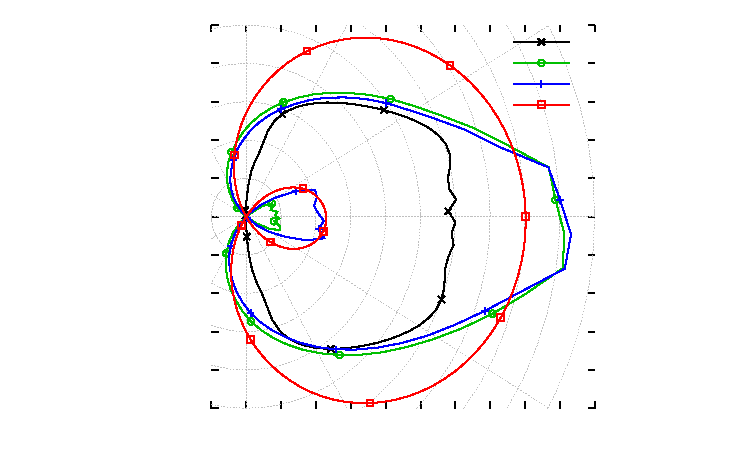
\includegraphics{/Users/seth/_thesis/figures/crashpipe2b/intens-x1-t1/intensity-x1-t1.pdf}}%
    \gplfronttext
  \end{picture}%
\endgroup

  \caption{Scalar flux with a normally incident boundary condition in a
  homogeneous flatland problem.}
  \label{fig:flatlandBcDelta}
\end{figure}
 
\begin{figure}[tb]
  \centering\small
  \hspace{-.25in}%
  % GNUPLOT: LaTeX picture with Postscript
\begingroup
  \makeatletter
  \providecommand\color[2][]{%
    \GenericError{(gnuplot) \space\space\space\@spaces}{%
      Package color not loaded in conjunction with
      terminal option `colourtext'%
    }{See the gnuplot documentation for explanation.%
    }{Either use 'blacktext' in gnuplot or load the package
      color.sty in LaTeX.}%
    \renewcommand\color[2][]{}%
  }%
  \providecommand\includegraphics[2][]{%
    \GenericError{(gnuplot) \space\space\space\@spaces}{%
      Package graphicx or graphics not loaded%
    }{See the gnuplot documentation for explanation.%
    }{The gnuplot epslatex terminal needs graphicx.sty or graphics.sty.}%
    \renewcommand\includegraphics[2][]{}%
  }%
  \providecommand\rotatebox[2]{#2}%
  \@ifundefined{ifGPcolor}{%
    \newif\ifGPcolor
    \GPcolortrue
  }{}%
  \@ifundefined{ifGPblacktext}{%
    \newif\ifGPblacktext
    \GPblacktexttrue
  }{}%
  % define a \g@addto@macro without @ in the name:
  \let\gplgaddtomacro\g@addto@macro
  % define empty templates for all commands taking text:
  \gdef\gplbacktext{}%
  \gdef\gplfronttext{}%
  \makeatother
  \ifGPblacktext
    % no textcolor at all
    \def\colorrgb#1{}%
    \def\colorgray#1{}%
  \else
    % gray or color?
    \ifGPcolor
      \def\colorrgb#1{\color[rgb]{#1}}%
      \def\colorgray#1{\color[gray]{#1}}%
      \expandafter\def\csname LTw\endcsname{\color{white}}%
      \expandafter\def\csname LTb\endcsname{\color{black}}%
      \expandafter\def\csname LTa\endcsname{\color{black}}%
      \expandafter\def\csname LT0\endcsname{\color[rgb]{1,0,0}}%
      \expandafter\def\csname LT1\endcsname{\color[rgb]{0,1,0}}%
      \expandafter\def\csname LT2\endcsname{\color[rgb]{0,0,1}}%
      \expandafter\def\csname LT3\endcsname{\color[rgb]{1,0,1}}%
      \expandafter\def\csname LT4\endcsname{\color[rgb]{0,1,1}}%
      \expandafter\def\csname LT5\endcsname{\color[rgb]{1,1,0}}%
      \expandafter\def\csname LT6\endcsname{\color[rgb]{0,0,0}}%
      \expandafter\def\csname LT7\endcsname{\color[rgb]{1,0.3,0}}%
      \expandafter\def\csname LT8\endcsname{\color[rgb]{0.5,0.5,0.5}}%
    \else
      % gray
      \def\colorrgb#1{\color{black}}%
      \def\colorgray#1{\color[gray]{#1}}%
      \expandafter\def\csname LTw\endcsname{\color{white}}%
      \expandafter\def\csname LTb\endcsname{\color{black}}%
      \expandafter\def\csname LTa\endcsname{\color{black}}%
      \expandafter\def\csname LT0\endcsname{\color{black}}%
      \expandafter\def\csname LT1\endcsname{\color{black}}%
      \expandafter\def\csname LT2\endcsname{\color{black}}%
      \expandafter\def\csname LT3\endcsname{\color{black}}%
      \expandafter\def\csname LT4\endcsname{\color{black}}%
      \expandafter\def\csname LT5\endcsname{\color{black}}%
      \expandafter\def\csname LT6\endcsname{\color{black}}%
      \expandafter\def\csname LT7\endcsname{\color{black}}%
      \expandafter\def\csname LT8\endcsname{\color{black}}%
    \fi
  \fi
  \setlength{\unitlength}{0.0500bp}%
  \begin{picture}(7200.00,4320.00)%
    \gplgaddtomacro\gplbacktext{%
      \csname LTb\endcsname%
      \put(1910,400){\makebox(0,0)[r]{\strut{} 0.1}}%
      \put(1910,768){\makebox(0,0)[r]{\strut{} 0.08}}%
      \put(1910,1136){\makebox(0,0)[r]{\strut{} 0.06}}%
      \put(1910,1504){\makebox(0,0)[r]{\strut{} 0.04}}%
      \put(1910,1872){\makebox(0,0)[r]{\strut{} 0.02}}%
      \put(1910,2240){\makebox(0,0)[r]{\strut{} 0}}%
      \put(1910,2607){\makebox(0,0)[r]{\strut{} 0.02}}%
      \put(1910,2975){\makebox(0,0)[r]{\strut{} 0.04}}%
      \put(1910,3343){\makebox(0,0)[r]{\strut{} 0.06}}%
      \put(1910,3711){\makebox(0,0)[r]{\strut{} 0.08}}%
      \put(1910,4079){\makebox(0,0)[r]{\strut{} 0.1}}%
      \csname LTb\endcsname%
      \put(2030,200){\makebox(0,0){\strut{} 0.02}}%
      \csname LTb\endcsname%
      \put(2364,200){\makebox(0,0){\strut{} 0}}%
      \csname LTb\endcsname%
      \put(2699,200){\makebox(0,0){\strut{} 0.02}}%
      \csname LTb\endcsname%
      \put(3033,200){\makebox(0,0){\strut{} 0.04}}%
      \csname LTb\endcsname%
      \put(3368,200){\makebox(0,0){\strut{} 0.06}}%
      \csname LTb\endcsname%
      \put(3702,200){\makebox(0,0){\strut{} 0.08}}%
      \csname LTb\endcsname%
      \put(4037,200){\makebox(0,0){\strut{} 0.1}}%
      \csname LTb\endcsname%
      \put(4371,200){\makebox(0,0){\strut{} 0.12}}%
      \csname LTb\endcsname%
      \put(4706,200){\makebox(0,0){\strut{} 0.14}}%
      \csname LTb\endcsname%
      \put(5040,200){\makebox(0,0){\strut{} 0.16}}%
      \csname LTb\endcsname%
      \put(5375,200){\makebox(0,0){\strut{} 0.18}}%
      \csname LTb\endcsname%
      \put(5709,200){\makebox(0,0){\strut{} 0.2}}%
      \csname LTb\endcsname%
      \put(1330,2239){\rotatebox{-270}{\makebox(0,0){\strut{}x1 center $(1.01,3.5)$}}}%
    }%
    \gplgaddtomacro\gplfronttext{%
      \csname LTb\endcsname%
      \put(4806,3916){\makebox(0,0)[r]{\strut{}S$_{128}$}}%
      \csname LTb\endcsname%
      \put(4806,3716){\makebox(0,0)[r]{\strut{}FLAD$_{64}$}}%
      \csname LTb\endcsname%
      \put(4806,3516){\makebox(0,0)[r]{\strut{}AD$_{64}$}}%
      \csname LTb\endcsname%
      \put(4806,3316){\makebox(0,0)[r]{\strut{}FLD}}%
    }%
    \gplbacktext
    \put(0,0){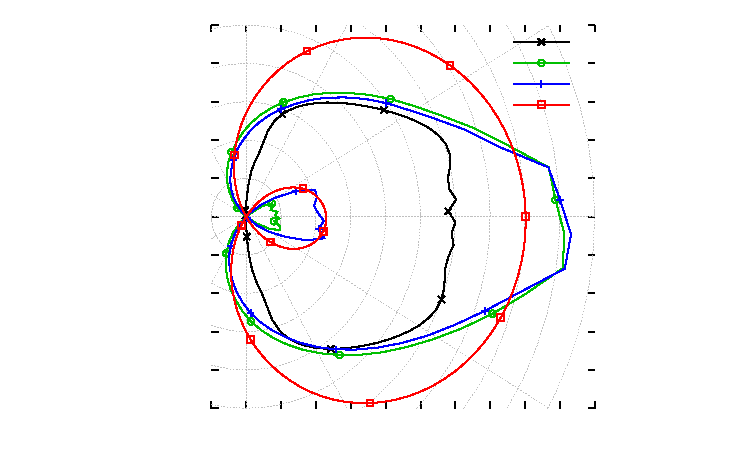
\includegraphics{/Users/seth/_thesis/figures/crashpipe2b/intens-x1-t1/intensity-x1-t1.pdf}}%
    \gplfronttext
  \end{picture}%
\endgroup

  \caption{Relative errors ($\phi/\phi_\text{MC} - 1$) of the three tested
  distributions.}
  \label{fig:flatlandBcRelative}
\end{figure}

%%%%%%%%%%%%%%%%%%%%%%%%%%%%%%%%%%%%%%%%%%%%%%%%%%%%%%%%%%%%%%%%%%%%%%%%%%%%%%%%
\section{Anisotropic diffusion boundary conditions}

In Chapter~\ref{chap:adDerivation}, we derived boundary conditions for the
anisotropic diffusion approximation. These boundary conditions reduce to the
standard diffusion boundary condition in a homogeneous medium, but they were
derived under a different set of asymptotic assumptions. We test the extent of
their applicability using several steady-state flatland test problem similar to
the above.

%%%%%%%%%%%%%%%%%%%%%%%%%%%%%%%%%%%%%%%%%%%%%%%%%%%%%%%%%%%%%%%%%%%%%%%%%%%%%%%%
\subsection{Interior source}

The first test of the anisotropic diffusion boundary conditions is a highly
scattering problem with a spatially smooth source in the interior. A vacuum
boundary in the problem serves as the primary sink for particles in the
problem; we therefore expect the global solution to be sensitive to the choice
of boundary conditions.

\subsubsection{Problem description}

The test problem (Fig.~\ref{fig:bcReactorProblem}) is similar to the above
%
\begin{figure}[htb]
  \centering
  \includegraphics{adbc-reactor/xsn-enhanced}
  \Caption{Steady-state AD boundary condition test problem.}{
    The black region is diffusive ($\sigma=1$, $\sigma_s=0.99$), the white
    region is optically thin ($\sigma=0.01$, $\sigma_s=0.0099$). The colored
    region in the lower-left is the Gaussian source.}
  \label{fig:bcReactorProblem}
\end{figure}
%
flatland boundary condition test
problem. It features a diffusive medium in flatland on the domain $0
\le x \le 5$ and $0 \le y \le 10$, with a channel of unit width running
vertically through the middle ($2.5 \le x \le 3.5$). The diffusive region has
$\sigma=1$ and $\sigma_s=0.99$, and the channel has $\sigma=0.01$ and
$\sigma_s=0.0099$. The bottom, left, and right boundaries are reflecting; the
top is a vacuum boundary.

The source is an isotropic Gaussian-shaped radiation source in the lower-left
corner:
\begin{equation*}
  q(x,y) = 2 \eexp^{-2 (x^2 + y^2) } \,.
\end{equation*}
The grid width used is $\Delta_x = \Delta_y = 0.1$.

We compare a Monte Carlo solution, a diffusion solution, and three instances of
anisotropic diffusion with different choices for the boundary condition on the
vacuum boundary. Only two---the white and reflecting
conditions---satisfy Eq.~\eqref{eq:hoBc}. The ``na\"ive'' boundary condition
sets the incident values of $f$ to zero and uses the Marshak diffusion boundary
condition from Eq.~\eqref{eq:flatMarshakAdBc}. It serves to demonstrate the
importance of using theoretically sound boundary conditions.

\subsubsection{Results and discussion}

First, we plot $f$ (Fig.~\ref{fig:bcReactorF}) at the top of the problem for
the three alternative boundary conditions for the purely absorbing transport
problem.

\begin{figure}[tb]
  \centering
  \subfloat[$f(2.5,10,\omega)$]{%
    \hspace{-.25in}%
    % GNUPLOT: LaTeX picture with Postscript
\begingroup
  \makeatletter
  \providecommand\color[2][]{%
    \GenericError{(gnuplot) \space\space\space\@spaces}{%
      Package color not loaded in conjunction with
      terminal option `colourtext'%
    }{See the gnuplot documentation for explanation.%
    }{Either use 'blacktext' in gnuplot or load the package
      color.sty in LaTeX.}%
    \renewcommand\color[2][]{}%
  }%
  \providecommand\includegraphics[2][]{%
    \GenericError{(gnuplot) \space\space\space\@spaces}{%
      Package graphicx or graphics not loaded%
    }{See the gnuplot documentation for explanation.%
    }{The gnuplot epslatex terminal needs graphicx.sty or graphics.sty.}%
    \renewcommand\includegraphics[2][]{}%
  }%
  \providecommand\rotatebox[2]{#2}%
  \@ifundefined{ifGPcolor}{%
    \newif\ifGPcolor
    \GPcolortrue
  }{}%
  \@ifundefined{ifGPblacktext}{%
    \newif\ifGPblacktext
    \GPblacktexttrue
  }{}%
  % define a \g@addto@macro without @ in the name:
  \let\gplgaddtomacro\g@addto@macro
  % define empty templates for all commands taking text:
  \gdef\gplbacktext{}%
  \gdef\gplfronttext{}%
  \makeatother
  \ifGPblacktext
    % no textcolor at all
    \def\colorrgb#1{}%
    \def\colorgray#1{}%
  \else
    % gray or color?
    \ifGPcolor
      \def\colorrgb#1{\color[rgb]{#1}}%
      \def\colorgray#1{\color[gray]{#1}}%
      \expandafter\def\csname LTw\endcsname{\color{white}}%
      \expandafter\def\csname LTb\endcsname{\color{black}}%
      \expandafter\def\csname LTa\endcsname{\color{black}}%
      \expandafter\def\csname LT0\endcsname{\color[rgb]{1,0,0}}%
      \expandafter\def\csname LT1\endcsname{\color[rgb]{0,1,0}}%
      \expandafter\def\csname LT2\endcsname{\color[rgb]{0,0,1}}%
      \expandafter\def\csname LT3\endcsname{\color[rgb]{1,0,1}}%
      \expandafter\def\csname LT4\endcsname{\color[rgb]{0,1,1}}%
      \expandafter\def\csname LT5\endcsname{\color[rgb]{1,1,0}}%
      \expandafter\def\csname LT6\endcsname{\color[rgb]{0,0,0}}%
      \expandafter\def\csname LT7\endcsname{\color[rgb]{1,0.3,0}}%
      \expandafter\def\csname LT8\endcsname{\color[rgb]{0.5,0.5,0.5}}%
    \else
      % gray
      \def\colorrgb#1{\color{black}}%
      \def\colorgray#1{\color[gray]{#1}}%
      \expandafter\def\csname LTw\endcsname{\color{white}}%
      \expandafter\def\csname LTb\endcsname{\color{black}}%
      \expandafter\def\csname LTa\endcsname{\color{black}}%
      \expandafter\def\csname LT0\endcsname{\color{black}}%
      \expandafter\def\csname LT1\endcsname{\color{black}}%
      \expandafter\def\csname LT2\endcsname{\color{black}}%
      \expandafter\def\csname LT3\endcsname{\color{black}}%
      \expandafter\def\csname LT4\endcsname{\color{black}}%
      \expandafter\def\csname LT5\endcsname{\color{black}}%
      \expandafter\def\csname LT6\endcsname{\color{black}}%
      \expandafter\def\csname LT7\endcsname{\color{black}}%
      \expandafter\def\csname LT8\endcsname{\color{black}}%
    \fi
  \fi
  \setlength{\unitlength}{0.0500bp}%
  \begin{picture}(7200.00,4320.00)%
    \gplgaddtomacro\gplbacktext{%
      \csname LTb\endcsname%
      \put(1910,400){\makebox(0,0)[r]{\strut{} 0.1}}%
      \put(1910,768){\makebox(0,0)[r]{\strut{} 0.08}}%
      \put(1910,1136){\makebox(0,0)[r]{\strut{} 0.06}}%
      \put(1910,1504){\makebox(0,0)[r]{\strut{} 0.04}}%
      \put(1910,1872){\makebox(0,0)[r]{\strut{} 0.02}}%
      \put(1910,2240){\makebox(0,0)[r]{\strut{} 0}}%
      \put(1910,2607){\makebox(0,0)[r]{\strut{} 0.02}}%
      \put(1910,2975){\makebox(0,0)[r]{\strut{} 0.04}}%
      \put(1910,3343){\makebox(0,0)[r]{\strut{} 0.06}}%
      \put(1910,3711){\makebox(0,0)[r]{\strut{} 0.08}}%
      \put(1910,4079){\makebox(0,0)[r]{\strut{} 0.1}}%
      \csname LTb\endcsname%
      \put(2030,200){\makebox(0,0){\strut{} 0.02}}%
      \csname LTb\endcsname%
      \put(2364,200){\makebox(0,0){\strut{} 0}}%
      \csname LTb\endcsname%
      \put(2699,200){\makebox(0,0){\strut{} 0.02}}%
      \csname LTb\endcsname%
      \put(3033,200){\makebox(0,0){\strut{} 0.04}}%
      \csname LTb\endcsname%
      \put(3368,200){\makebox(0,0){\strut{} 0.06}}%
      \csname LTb\endcsname%
      \put(3702,200){\makebox(0,0){\strut{} 0.08}}%
      \csname LTb\endcsname%
      \put(4037,200){\makebox(0,0){\strut{} 0.1}}%
      \csname LTb\endcsname%
      \put(4371,200){\makebox(0,0){\strut{} 0.12}}%
      \csname LTb\endcsname%
      \put(4706,200){\makebox(0,0){\strut{} 0.14}}%
      \csname LTb\endcsname%
      \put(5040,200){\makebox(0,0){\strut{} 0.16}}%
      \csname LTb\endcsname%
      \put(5375,200){\makebox(0,0){\strut{} 0.18}}%
      \csname LTb\endcsname%
      \put(5709,200){\makebox(0,0){\strut{} 0.2}}%
      \csname LTb\endcsname%
      \put(1330,2239){\rotatebox{-270}{\makebox(0,0){\strut{}x1 center $(1.01,3.5)$}}}%
    }%
    \gplgaddtomacro\gplfronttext{%
      \csname LTb\endcsname%
      \put(4806,3916){\makebox(0,0)[r]{\strut{}S$_{128}$}}%
      \csname LTb\endcsname%
      \put(4806,3716){\makebox(0,0)[r]{\strut{}FLAD$_{64}$}}%
      \csname LTb\endcsname%
      \put(4806,3516){\makebox(0,0)[r]{\strut{}AD$_{64}$}}%
      \csname LTb\endcsname%
      \put(4806,3316){\makebox(0,0)[r]{\strut{}FLD}}%
    }%
    \gplbacktext
    \put(0,0){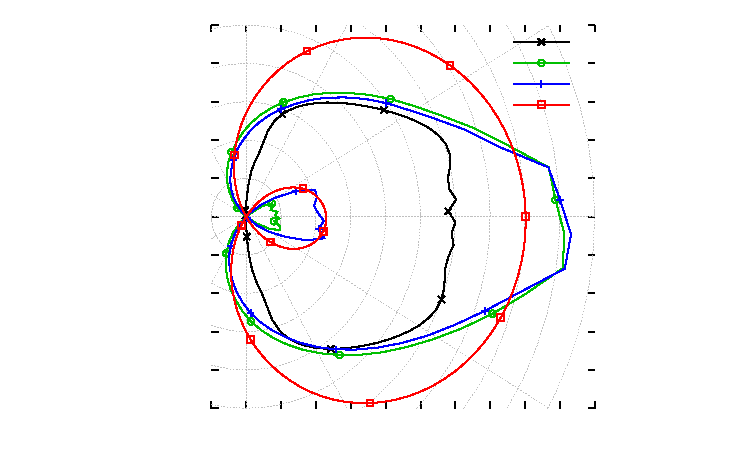
\includegraphics{/Users/seth/_thesis/figures/crashpipe2b/intens-x1-t1/intensity-x1-t1.pdf}}%
    \gplfronttext
  \end{picture}%
\endgroup
%
   \label{fig:bcReactorFchan}%
  }%
  \subfloat[$f(1.5,10,\omega)$]{%
    \hspace{-.25in}%
    % GNUPLOT: LaTeX picture with Postscript
\begingroup
  \makeatletter
  \providecommand\color[2][]{%
    \GenericError{(gnuplot) \space\space\space\@spaces}{%
      Package color not loaded in conjunction with
      terminal option `colourtext'%
    }{See the gnuplot documentation for explanation.%
    }{Either use 'blacktext' in gnuplot or load the package
      color.sty in LaTeX.}%
    \renewcommand\color[2][]{}%
  }%
  \providecommand\includegraphics[2][]{%
    \GenericError{(gnuplot) \space\space\space\@spaces}{%
      Package graphicx or graphics not loaded%
    }{See the gnuplot documentation for explanation.%
    }{The gnuplot epslatex terminal needs graphicx.sty or graphics.sty.}%
    \renewcommand\includegraphics[2][]{}%
  }%
  \providecommand\rotatebox[2]{#2}%
  \@ifundefined{ifGPcolor}{%
    \newif\ifGPcolor
    \GPcolortrue
  }{}%
  \@ifundefined{ifGPblacktext}{%
    \newif\ifGPblacktext
    \GPblacktexttrue
  }{}%
  % define a \g@addto@macro without @ in the name:
  \let\gplgaddtomacro\g@addto@macro
  % define empty templates for all commands taking text:
  \gdef\gplbacktext{}%
  \gdef\gplfronttext{}%
  \makeatother
  \ifGPblacktext
    % no textcolor at all
    \def\colorrgb#1{}%
    \def\colorgray#1{}%
  \else
    % gray or color?
    \ifGPcolor
      \def\colorrgb#1{\color[rgb]{#1}}%
      \def\colorgray#1{\color[gray]{#1}}%
      \expandafter\def\csname LTw\endcsname{\color{white}}%
      \expandafter\def\csname LTb\endcsname{\color{black}}%
      \expandafter\def\csname LTa\endcsname{\color{black}}%
      \expandafter\def\csname LT0\endcsname{\color[rgb]{1,0,0}}%
      \expandafter\def\csname LT1\endcsname{\color[rgb]{0,1,0}}%
      \expandafter\def\csname LT2\endcsname{\color[rgb]{0,0,1}}%
      \expandafter\def\csname LT3\endcsname{\color[rgb]{1,0,1}}%
      \expandafter\def\csname LT4\endcsname{\color[rgb]{0,1,1}}%
      \expandafter\def\csname LT5\endcsname{\color[rgb]{1,1,0}}%
      \expandafter\def\csname LT6\endcsname{\color[rgb]{0,0,0}}%
      \expandafter\def\csname LT7\endcsname{\color[rgb]{1,0.3,0}}%
      \expandafter\def\csname LT8\endcsname{\color[rgb]{0.5,0.5,0.5}}%
    \else
      % gray
      \def\colorrgb#1{\color{black}}%
      \def\colorgray#1{\color[gray]{#1}}%
      \expandafter\def\csname LTw\endcsname{\color{white}}%
      \expandafter\def\csname LTb\endcsname{\color{black}}%
      \expandafter\def\csname LTa\endcsname{\color{black}}%
      \expandafter\def\csname LT0\endcsname{\color{black}}%
      \expandafter\def\csname LT1\endcsname{\color{black}}%
      \expandafter\def\csname LT2\endcsname{\color{black}}%
      \expandafter\def\csname LT3\endcsname{\color{black}}%
      \expandafter\def\csname LT4\endcsname{\color{black}}%
      \expandafter\def\csname LT5\endcsname{\color{black}}%
      \expandafter\def\csname LT6\endcsname{\color{black}}%
      \expandafter\def\csname LT7\endcsname{\color{black}}%
      \expandafter\def\csname LT8\endcsname{\color{black}}%
    \fi
  \fi
  \setlength{\unitlength}{0.0500bp}%
  \begin{picture}(7200.00,4320.00)%
    \gplgaddtomacro\gplbacktext{%
      \csname LTb\endcsname%
      \put(1910,400){\makebox(0,0)[r]{\strut{} 0.1}}%
      \put(1910,768){\makebox(0,0)[r]{\strut{} 0.08}}%
      \put(1910,1136){\makebox(0,0)[r]{\strut{} 0.06}}%
      \put(1910,1504){\makebox(0,0)[r]{\strut{} 0.04}}%
      \put(1910,1872){\makebox(0,0)[r]{\strut{} 0.02}}%
      \put(1910,2240){\makebox(0,0)[r]{\strut{} 0}}%
      \put(1910,2607){\makebox(0,0)[r]{\strut{} 0.02}}%
      \put(1910,2975){\makebox(0,0)[r]{\strut{} 0.04}}%
      \put(1910,3343){\makebox(0,0)[r]{\strut{} 0.06}}%
      \put(1910,3711){\makebox(0,0)[r]{\strut{} 0.08}}%
      \put(1910,4079){\makebox(0,0)[r]{\strut{} 0.1}}%
      \csname LTb\endcsname%
      \put(2030,200){\makebox(0,0){\strut{} 0.02}}%
      \csname LTb\endcsname%
      \put(2364,200){\makebox(0,0){\strut{} 0}}%
      \csname LTb\endcsname%
      \put(2699,200){\makebox(0,0){\strut{} 0.02}}%
      \csname LTb\endcsname%
      \put(3033,200){\makebox(0,0){\strut{} 0.04}}%
      \csname LTb\endcsname%
      \put(3368,200){\makebox(0,0){\strut{} 0.06}}%
      \csname LTb\endcsname%
      \put(3702,200){\makebox(0,0){\strut{} 0.08}}%
      \csname LTb\endcsname%
      \put(4037,200){\makebox(0,0){\strut{} 0.1}}%
      \csname LTb\endcsname%
      \put(4371,200){\makebox(0,0){\strut{} 0.12}}%
      \csname LTb\endcsname%
      \put(4706,200){\makebox(0,0){\strut{} 0.14}}%
      \csname LTb\endcsname%
      \put(5040,200){\makebox(0,0){\strut{} 0.16}}%
      \csname LTb\endcsname%
      \put(5375,200){\makebox(0,0){\strut{} 0.18}}%
      \csname LTb\endcsname%
      \put(5709,200){\makebox(0,0){\strut{} 0.2}}%
      \csname LTb\endcsname%
      \put(1330,2239){\rotatebox{-270}{\makebox(0,0){\strut{}x1 center $(1.01,3.5)$}}}%
    }%
    \gplgaddtomacro\gplfronttext{%
      \csname LTb\endcsname%
      \put(4806,3916){\makebox(0,0)[r]{\strut{}S$_{128}$}}%
      \csname LTb\endcsname%
      \put(4806,3716){\makebox(0,0)[r]{\strut{}FLAD$_{64}$}}%
      \csname LTb\endcsname%
      \put(4806,3516){\makebox(0,0)[r]{\strut{}AD$_{64}$}}%
      \csname LTb\endcsname%
      \put(4806,3316){\makebox(0,0)[r]{\strut{}FLD}}%
    }%
    \gplbacktext
    \put(0,0){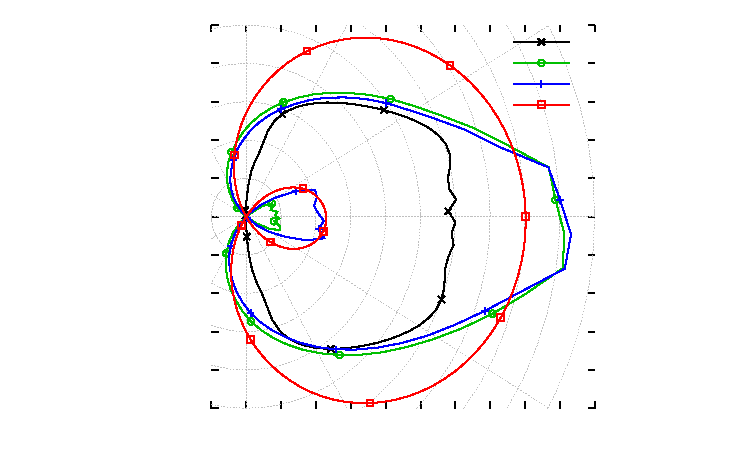
\includegraphics{/Users/seth/_thesis/figures/crashpipe2b/intens-x1-t1/intensity-x1-t1.pdf}}%
    \gplfronttext
  \end{picture}%
\endgroup

  }%
  \Caption{Plots of the purely absorbing transport solution at two points in
  at the end of the channel.}{
  The center of the channel (a) shows the highly anisotropic behavior $f$ can
  take; further from material discontinuities (b), $f$ tends toward isotropy.
  }
  \label{fig:bcReactorF}
\end{figure}

The effect of the boundary condition on $f$ is straightforward: a reflecting boundary
condition mirrors the angular distribution across the $x$ axis, and a white
boundary condition yields an isotropic distribution for incident angles. The
na\"ive boundary condition is positive only for exiting angles. For the sake of
comparison, the diffusion approximation $f(\vec{x},\vec{\Omega}) =
\frac{1}{2\pi \sigma(\vec{x})}$ could be plotted as a circle. (In
Fig.~\ref{fig:bcReactorFchan}, it would be out of range of the plot.) Both the
anisotropic diffusion tensor $\Dtens$ and the boundary coefficient
$\vec{d}$ change as a result of the boundary conditions.

The different diffusion and boundary coefficients naturally cause the
anisotropic diffusion solutions $\phi$ to differ. Figure~\ref{fig:bcReactorFlux}
compares the three instances of anisotropic diffusion with the Monte Carlo
reference solution and the diffusion solution.

\begin{figure}[htb]
  \centering
  \hspace{-.25in}%
  % GNUPLOT: LaTeX picture with Postscript
\begingroup
  \makeatletter
  \providecommand\color[2][]{%
    \GenericError{(gnuplot) \space\space\space\@spaces}{%
      Package color not loaded in conjunction with
      terminal option `colourtext'%
    }{See the gnuplot documentation for explanation.%
    }{Either use 'blacktext' in gnuplot or load the package
      color.sty in LaTeX.}%
    \renewcommand\color[2][]{}%
  }%
  \providecommand\includegraphics[2][]{%
    \GenericError{(gnuplot) \space\space\space\@spaces}{%
      Package graphicx or graphics not loaded%
    }{See the gnuplot documentation for explanation.%
    }{The gnuplot epslatex terminal needs graphicx.sty or graphics.sty.}%
    \renewcommand\includegraphics[2][]{}%
  }%
  \providecommand\rotatebox[2]{#2}%
  \@ifundefined{ifGPcolor}{%
    \newif\ifGPcolor
    \GPcolortrue
  }{}%
  \@ifundefined{ifGPblacktext}{%
    \newif\ifGPblacktext
    \GPblacktexttrue
  }{}%
  % define a \g@addto@macro without @ in the name:
  \let\gplgaddtomacro\g@addto@macro
  % define empty templates for all commands taking text:
  \gdef\gplbacktext{}%
  \gdef\gplfronttext{}%
  \makeatother
  \ifGPblacktext
    % no textcolor at all
    \def\colorrgb#1{}%
    \def\colorgray#1{}%
  \else
    % gray or color?
    \ifGPcolor
      \def\colorrgb#1{\color[rgb]{#1}}%
      \def\colorgray#1{\color[gray]{#1}}%
      \expandafter\def\csname LTw\endcsname{\color{white}}%
      \expandafter\def\csname LTb\endcsname{\color{black}}%
      \expandafter\def\csname LTa\endcsname{\color{black}}%
      \expandafter\def\csname LT0\endcsname{\color[rgb]{1,0,0}}%
      \expandafter\def\csname LT1\endcsname{\color[rgb]{0,1,0}}%
      \expandafter\def\csname LT2\endcsname{\color[rgb]{0,0,1}}%
      \expandafter\def\csname LT3\endcsname{\color[rgb]{1,0,1}}%
      \expandafter\def\csname LT4\endcsname{\color[rgb]{0,1,1}}%
      \expandafter\def\csname LT5\endcsname{\color[rgb]{1,1,0}}%
      \expandafter\def\csname LT6\endcsname{\color[rgb]{0,0,0}}%
      \expandafter\def\csname LT7\endcsname{\color[rgb]{1,0.3,0}}%
      \expandafter\def\csname LT8\endcsname{\color[rgb]{0.5,0.5,0.5}}%
    \else
      % gray
      \def\colorrgb#1{\color{black}}%
      \def\colorgray#1{\color[gray]{#1}}%
      \expandafter\def\csname LTw\endcsname{\color{white}}%
      \expandafter\def\csname LTb\endcsname{\color{black}}%
      \expandafter\def\csname LTa\endcsname{\color{black}}%
      \expandafter\def\csname LT0\endcsname{\color{black}}%
      \expandafter\def\csname LT1\endcsname{\color{black}}%
      \expandafter\def\csname LT2\endcsname{\color{black}}%
      \expandafter\def\csname LT3\endcsname{\color{black}}%
      \expandafter\def\csname LT4\endcsname{\color{black}}%
      \expandafter\def\csname LT5\endcsname{\color{black}}%
      \expandafter\def\csname LT6\endcsname{\color{black}}%
      \expandafter\def\csname LT7\endcsname{\color{black}}%
      \expandafter\def\csname LT8\endcsname{\color{black}}%
    \fi
  \fi
  \setlength{\unitlength}{0.0500bp}%
  \begin{picture}(7200.00,4320.00)%
    \gplgaddtomacro\gplbacktext{%
      \csname LTb\endcsname%
      \put(1910,400){\makebox(0,0)[r]{\strut{} 0.1}}%
      \put(1910,768){\makebox(0,0)[r]{\strut{} 0.08}}%
      \put(1910,1136){\makebox(0,0)[r]{\strut{} 0.06}}%
      \put(1910,1504){\makebox(0,0)[r]{\strut{} 0.04}}%
      \put(1910,1872){\makebox(0,0)[r]{\strut{} 0.02}}%
      \put(1910,2240){\makebox(0,0)[r]{\strut{} 0}}%
      \put(1910,2607){\makebox(0,0)[r]{\strut{} 0.02}}%
      \put(1910,2975){\makebox(0,0)[r]{\strut{} 0.04}}%
      \put(1910,3343){\makebox(0,0)[r]{\strut{} 0.06}}%
      \put(1910,3711){\makebox(0,0)[r]{\strut{} 0.08}}%
      \put(1910,4079){\makebox(0,0)[r]{\strut{} 0.1}}%
      \csname LTb\endcsname%
      \put(2030,200){\makebox(0,0){\strut{} 0.02}}%
      \csname LTb\endcsname%
      \put(2364,200){\makebox(0,0){\strut{} 0}}%
      \csname LTb\endcsname%
      \put(2699,200){\makebox(0,0){\strut{} 0.02}}%
      \csname LTb\endcsname%
      \put(3033,200){\makebox(0,0){\strut{} 0.04}}%
      \csname LTb\endcsname%
      \put(3368,200){\makebox(0,0){\strut{} 0.06}}%
      \csname LTb\endcsname%
      \put(3702,200){\makebox(0,0){\strut{} 0.08}}%
      \csname LTb\endcsname%
      \put(4037,200){\makebox(0,0){\strut{} 0.1}}%
      \csname LTb\endcsname%
      \put(4371,200){\makebox(0,0){\strut{} 0.12}}%
      \csname LTb\endcsname%
      \put(4706,200){\makebox(0,0){\strut{} 0.14}}%
      \csname LTb\endcsname%
      \put(5040,200){\makebox(0,0){\strut{} 0.16}}%
      \csname LTb\endcsname%
      \put(5375,200){\makebox(0,0){\strut{} 0.18}}%
      \csname LTb\endcsname%
      \put(5709,200){\makebox(0,0){\strut{} 0.2}}%
      \csname LTb\endcsname%
      \put(1330,2239){\rotatebox{-270}{\makebox(0,0){\strut{}x1 center $(1.01,3.5)$}}}%
    }%
    \gplgaddtomacro\gplfronttext{%
      \csname LTb\endcsname%
      \put(4806,3916){\makebox(0,0)[r]{\strut{}S$_{128}$}}%
      \csname LTb\endcsname%
      \put(4806,3716){\makebox(0,0)[r]{\strut{}FLAD$_{64}$}}%
      \csname LTb\endcsname%
      \put(4806,3516){\makebox(0,0)[r]{\strut{}AD$_{64}$}}%
      \csname LTb\endcsname%
      \put(4806,3316){\makebox(0,0)[r]{\strut{}FLD}}%
    }%
    \gplbacktext
    \put(0,0){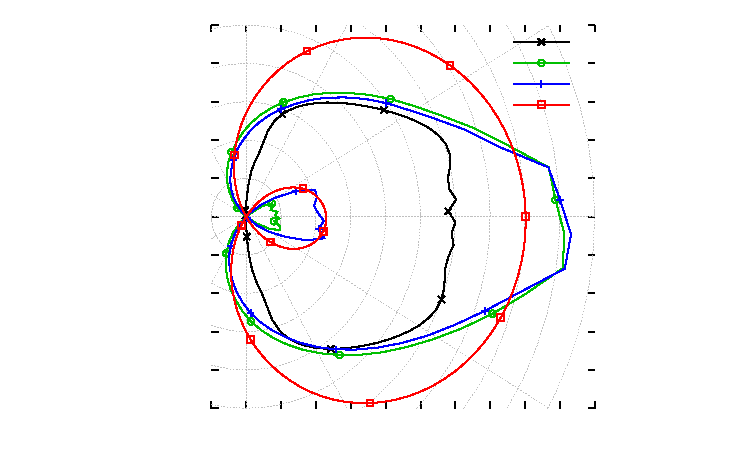
\includegraphics{/Users/seth/_thesis/figures/crashpipe2b/intens-x1-t1/intensity-x1-t1.pdf}}%
    \gplfronttext
  \end{picture}%
\endgroup

  \caption{Scalar flux in the steady-state interior source problem.}
  \label{fig:bcReactorFlux}
\end{figure}

Clearly, anisotropic diffusion is superior to conventional diffusion: it differs
from the reference solution by only few percent globally. The two choices of
boundary conditions for $f$ consistent with Eq.~\eqref{eq:hoBc}, reflecting and
white, produce very similar answers. In contrast, the inconsistent choice of a
vacuum boundary for $f$ introduces a significant global error, even many mean
free paths away from the boundary.

To help understand the accuracy of anisotropic diffusion as compared to standard
diffusion, we have plotted in Fig.~\ref{fig:bcReactorAngular} the angular
intensity at several points in the problem as approximated by \SN, AD, and
standard diffusion. Whereas standard diffusion approximates the radiation as linear in
angle, anisotropic diffusion has much more \emph{shape}, resulting from the
(generally nonlinear)
anisotropy in $f$. As we asserted in Chapter~\ref{chap:adDerivation}, this extra
transport-derived information results in a more accurate approximation.

\begin{figure}[htb]
  \centering\small
  \subfloat[$\psi(2.5,0,\omega)$]{%
    \hspace{-.25in}%
    % GNUPLOT: LaTeX picture with Postscript
\begingroup
  \makeatletter
  \providecommand\color[2][]{%
    \GenericError{(gnuplot) \space\space\space\@spaces}{%
      Package color not loaded in conjunction with
      terminal option `colourtext'%
    }{See the gnuplot documentation for explanation.%
    }{Either use 'blacktext' in gnuplot or load the package
      color.sty in LaTeX.}%
    \renewcommand\color[2][]{}%
  }%
  \providecommand\includegraphics[2][]{%
    \GenericError{(gnuplot) \space\space\space\@spaces}{%
      Package graphicx or graphics not loaded%
    }{See the gnuplot documentation for explanation.%
    }{The gnuplot epslatex terminal needs graphicx.sty or graphics.sty.}%
    \renewcommand\includegraphics[2][]{}%
  }%
  \providecommand\rotatebox[2]{#2}%
  \@ifundefined{ifGPcolor}{%
    \newif\ifGPcolor
    \GPcolortrue
  }{}%
  \@ifundefined{ifGPblacktext}{%
    \newif\ifGPblacktext
    \GPblacktexttrue
  }{}%
  % define a \g@addto@macro without @ in the name:
  \let\gplgaddtomacro\g@addto@macro
  % define empty templates for all commands taking text:
  \gdef\gplbacktext{}%
  \gdef\gplfronttext{}%
  \makeatother
  \ifGPblacktext
    % no textcolor at all
    \def\colorrgb#1{}%
    \def\colorgray#1{}%
  \else
    % gray or color?
    \ifGPcolor
      \def\colorrgb#1{\color[rgb]{#1}}%
      \def\colorgray#1{\color[gray]{#1}}%
      \expandafter\def\csname LTw\endcsname{\color{white}}%
      \expandafter\def\csname LTb\endcsname{\color{black}}%
      \expandafter\def\csname LTa\endcsname{\color{black}}%
      \expandafter\def\csname LT0\endcsname{\color[rgb]{1,0,0}}%
      \expandafter\def\csname LT1\endcsname{\color[rgb]{0,1,0}}%
      \expandafter\def\csname LT2\endcsname{\color[rgb]{0,0,1}}%
      \expandafter\def\csname LT3\endcsname{\color[rgb]{1,0,1}}%
      \expandafter\def\csname LT4\endcsname{\color[rgb]{0,1,1}}%
      \expandafter\def\csname LT5\endcsname{\color[rgb]{1,1,0}}%
      \expandafter\def\csname LT6\endcsname{\color[rgb]{0,0,0}}%
      \expandafter\def\csname LT7\endcsname{\color[rgb]{1,0.3,0}}%
      \expandafter\def\csname LT8\endcsname{\color[rgb]{0.5,0.5,0.5}}%
    \else
      % gray
      \def\colorrgb#1{\color{black}}%
      \def\colorgray#1{\color[gray]{#1}}%
      \expandafter\def\csname LTw\endcsname{\color{white}}%
      \expandafter\def\csname LTb\endcsname{\color{black}}%
      \expandafter\def\csname LTa\endcsname{\color{black}}%
      \expandafter\def\csname LT0\endcsname{\color{black}}%
      \expandafter\def\csname LT1\endcsname{\color{black}}%
      \expandafter\def\csname LT2\endcsname{\color{black}}%
      \expandafter\def\csname LT3\endcsname{\color{black}}%
      \expandafter\def\csname LT4\endcsname{\color{black}}%
      \expandafter\def\csname LT5\endcsname{\color{black}}%
      \expandafter\def\csname LT6\endcsname{\color{black}}%
      \expandafter\def\csname LT7\endcsname{\color{black}}%
      \expandafter\def\csname LT8\endcsname{\color{black}}%
    \fi
  \fi
  \setlength{\unitlength}{0.0500bp}%
  \begin{picture}(7200.00,4320.00)%
    \gplgaddtomacro\gplbacktext{%
      \csname LTb\endcsname%
      \put(1910,400){\makebox(0,0)[r]{\strut{} 0.1}}%
      \put(1910,768){\makebox(0,0)[r]{\strut{} 0.08}}%
      \put(1910,1136){\makebox(0,0)[r]{\strut{} 0.06}}%
      \put(1910,1504){\makebox(0,0)[r]{\strut{} 0.04}}%
      \put(1910,1872){\makebox(0,0)[r]{\strut{} 0.02}}%
      \put(1910,2240){\makebox(0,0)[r]{\strut{} 0}}%
      \put(1910,2607){\makebox(0,0)[r]{\strut{} 0.02}}%
      \put(1910,2975){\makebox(0,0)[r]{\strut{} 0.04}}%
      \put(1910,3343){\makebox(0,0)[r]{\strut{} 0.06}}%
      \put(1910,3711){\makebox(0,0)[r]{\strut{} 0.08}}%
      \put(1910,4079){\makebox(0,0)[r]{\strut{} 0.1}}%
      \csname LTb\endcsname%
      \put(2030,200){\makebox(0,0){\strut{} 0.02}}%
      \csname LTb\endcsname%
      \put(2364,200){\makebox(0,0){\strut{} 0}}%
      \csname LTb\endcsname%
      \put(2699,200){\makebox(0,0){\strut{} 0.02}}%
      \csname LTb\endcsname%
      \put(3033,200){\makebox(0,0){\strut{} 0.04}}%
      \csname LTb\endcsname%
      \put(3368,200){\makebox(0,0){\strut{} 0.06}}%
      \csname LTb\endcsname%
      \put(3702,200){\makebox(0,0){\strut{} 0.08}}%
      \csname LTb\endcsname%
      \put(4037,200){\makebox(0,0){\strut{} 0.1}}%
      \csname LTb\endcsname%
      \put(4371,200){\makebox(0,0){\strut{} 0.12}}%
      \csname LTb\endcsname%
      \put(4706,200){\makebox(0,0){\strut{} 0.14}}%
      \csname LTb\endcsname%
      \put(5040,200){\makebox(0,0){\strut{} 0.16}}%
      \csname LTb\endcsname%
      \put(5375,200){\makebox(0,0){\strut{} 0.18}}%
      \csname LTb\endcsname%
      \put(5709,200){\makebox(0,0){\strut{} 0.2}}%
      \csname LTb\endcsname%
      \put(1330,2239){\rotatebox{-270}{\makebox(0,0){\strut{}x1 center $(1.01,3.5)$}}}%
    }%
    \gplgaddtomacro\gplfronttext{%
      \csname LTb\endcsname%
      \put(4806,3916){\makebox(0,0)[r]{\strut{}S$_{128}$}}%
      \csname LTb\endcsname%
      \put(4806,3716){\makebox(0,0)[r]{\strut{}FLAD$_{64}$}}%
      \csname LTb\endcsname%
      \put(4806,3516){\makebox(0,0)[r]{\strut{}AD$_{64}$}}%
      \csname LTb\endcsname%
      \put(4806,3316){\makebox(0,0)[r]{\strut{}FLD}}%
    }%
    \gplbacktext
    \put(0,0){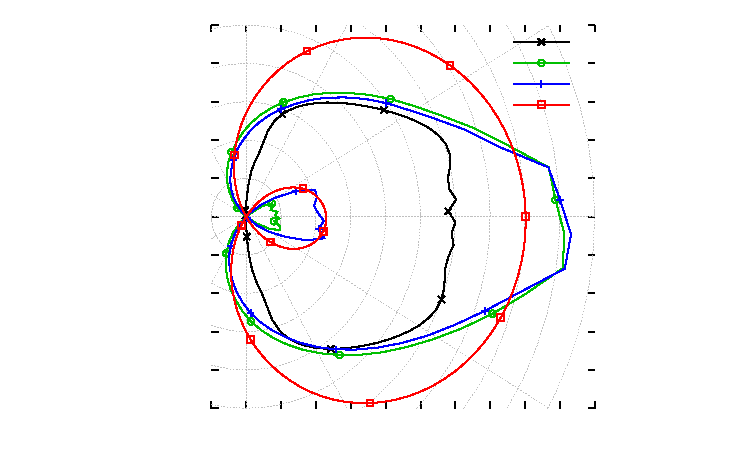
\includegraphics{/Users/seth/_thesis/figures/crashpipe2b/intens-x1-t1/intensity-x1-t1.pdf}}%
    \gplfronttext
  \end{picture}%
\endgroup
}

  \subfloat[$\psi(2.5,10,\omega)$]{%
    \hspace{-.25in}%
    % GNUPLOT: LaTeX picture with Postscript
\begingroup
  \makeatletter
  \providecommand\color[2][]{%
    \GenericError{(gnuplot) \space\space\space\@spaces}{%
      Package color not loaded in conjunction with
      terminal option `colourtext'%
    }{See the gnuplot documentation for explanation.%
    }{Either use 'blacktext' in gnuplot or load the package
      color.sty in LaTeX.}%
    \renewcommand\color[2][]{}%
  }%
  \providecommand\includegraphics[2][]{%
    \GenericError{(gnuplot) \space\space\space\@spaces}{%
      Package graphicx or graphics not loaded%
    }{See the gnuplot documentation for explanation.%
    }{The gnuplot epslatex terminal needs graphicx.sty or graphics.sty.}%
    \renewcommand\includegraphics[2][]{}%
  }%
  \providecommand\rotatebox[2]{#2}%
  \@ifundefined{ifGPcolor}{%
    \newif\ifGPcolor
    \GPcolortrue
  }{}%
  \@ifundefined{ifGPblacktext}{%
    \newif\ifGPblacktext
    \GPblacktexttrue
  }{}%
  % define a \g@addto@macro without @ in the name:
  \let\gplgaddtomacro\g@addto@macro
  % define empty templates for all commands taking text:
  \gdef\gplbacktext{}%
  \gdef\gplfronttext{}%
  \makeatother
  \ifGPblacktext
    % no textcolor at all
    \def\colorrgb#1{}%
    \def\colorgray#1{}%
  \else
    % gray or color?
    \ifGPcolor
      \def\colorrgb#1{\color[rgb]{#1}}%
      \def\colorgray#1{\color[gray]{#1}}%
      \expandafter\def\csname LTw\endcsname{\color{white}}%
      \expandafter\def\csname LTb\endcsname{\color{black}}%
      \expandafter\def\csname LTa\endcsname{\color{black}}%
      \expandafter\def\csname LT0\endcsname{\color[rgb]{1,0,0}}%
      \expandafter\def\csname LT1\endcsname{\color[rgb]{0,1,0}}%
      \expandafter\def\csname LT2\endcsname{\color[rgb]{0,0,1}}%
      \expandafter\def\csname LT3\endcsname{\color[rgb]{1,0,1}}%
      \expandafter\def\csname LT4\endcsname{\color[rgb]{0,1,1}}%
      \expandafter\def\csname LT5\endcsname{\color[rgb]{1,1,0}}%
      \expandafter\def\csname LT6\endcsname{\color[rgb]{0,0,0}}%
      \expandafter\def\csname LT7\endcsname{\color[rgb]{1,0.3,0}}%
      \expandafter\def\csname LT8\endcsname{\color[rgb]{0.5,0.5,0.5}}%
    \else
      % gray
      \def\colorrgb#1{\color{black}}%
      \def\colorgray#1{\color[gray]{#1}}%
      \expandafter\def\csname LTw\endcsname{\color{white}}%
      \expandafter\def\csname LTb\endcsname{\color{black}}%
      \expandafter\def\csname LTa\endcsname{\color{black}}%
      \expandafter\def\csname LT0\endcsname{\color{black}}%
      \expandafter\def\csname LT1\endcsname{\color{black}}%
      \expandafter\def\csname LT2\endcsname{\color{black}}%
      \expandafter\def\csname LT3\endcsname{\color{black}}%
      \expandafter\def\csname LT4\endcsname{\color{black}}%
      \expandafter\def\csname LT5\endcsname{\color{black}}%
      \expandafter\def\csname LT6\endcsname{\color{black}}%
      \expandafter\def\csname LT7\endcsname{\color{black}}%
      \expandafter\def\csname LT8\endcsname{\color{black}}%
    \fi
  \fi
  \setlength{\unitlength}{0.0500bp}%
  \begin{picture}(7200.00,4320.00)%
    \gplgaddtomacro\gplbacktext{%
      \csname LTb\endcsname%
      \put(1910,400){\makebox(0,0)[r]{\strut{} 0.1}}%
      \put(1910,768){\makebox(0,0)[r]{\strut{} 0.08}}%
      \put(1910,1136){\makebox(0,0)[r]{\strut{} 0.06}}%
      \put(1910,1504){\makebox(0,0)[r]{\strut{} 0.04}}%
      \put(1910,1872){\makebox(0,0)[r]{\strut{} 0.02}}%
      \put(1910,2240){\makebox(0,0)[r]{\strut{} 0}}%
      \put(1910,2607){\makebox(0,0)[r]{\strut{} 0.02}}%
      \put(1910,2975){\makebox(0,0)[r]{\strut{} 0.04}}%
      \put(1910,3343){\makebox(0,0)[r]{\strut{} 0.06}}%
      \put(1910,3711){\makebox(0,0)[r]{\strut{} 0.08}}%
      \put(1910,4079){\makebox(0,0)[r]{\strut{} 0.1}}%
      \csname LTb\endcsname%
      \put(2030,200){\makebox(0,0){\strut{} 0.02}}%
      \csname LTb\endcsname%
      \put(2364,200){\makebox(0,0){\strut{} 0}}%
      \csname LTb\endcsname%
      \put(2699,200){\makebox(0,0){\strut{} 0.02}}%
      \csname LTb\endcsname%
      \put(3033,200){\makebox(0,0){\strut{} 0.04}}%
      \csname LTb\endcsname%
      \put(3368,200){\makebox(0,0){\strut{} 0.06}}%
      \csname LTb\endcsname%
      \put(3702,200){\makebox(0,0){\strut{} 0.08}}%
      \csname LTb\endcsname%
      \put(4037,200){\makebox(0,0){\strut{} 0.1}}%
      \csname LTb\endcsname%
      \put(4371,200){\makebox(0,0){\strut{} 0.12}}%
      \csname LTb\endcsname%
      \put(4706,200){\makebox(0,0){\strut{} 0.14}}%
      \csname LTb\endcsname%
      \put(5040,200){\makebox(0,0){\strut{} 0.16}}%
      \csname LTb\endcsname%
      \put(5375,200){\makebox(0,0){\strut{} 0.18}}%
      \csname LTb\endcsname%
      \put(5709,200){\makebox(0,0){\strut{} 0.2}}%
      \csname LTb\endcsname%
      \put(1330,2239){\rotatebox{-270}{\makebox(0,0){\strut{}x1 center $(1.01,3.5)$}}}%
    }%
    \gplgaddtomacro\gplfronttext{%
      \csname LTb\endcsname%
      \put(4806,3916){\makebox(0,0)[r]{\strut{}S$_{128}$}}%
      \csname LTb\endcsname%
      \put(4806,3716){\makebox(0,0)[r]{\strut{}FLAD$_{64}$}}%
      \csname LTb\endcsname%
      \put(4806,3516){\makebox(0,0)[r]{\strut{}AD$_{64}$}}%
      \csname LTb\endcsname%
      \put(4806,3316){\makebox(0,0)[r]{\strut{}FLD}}%
    }%
    \gplbacktext
    \put(0,0){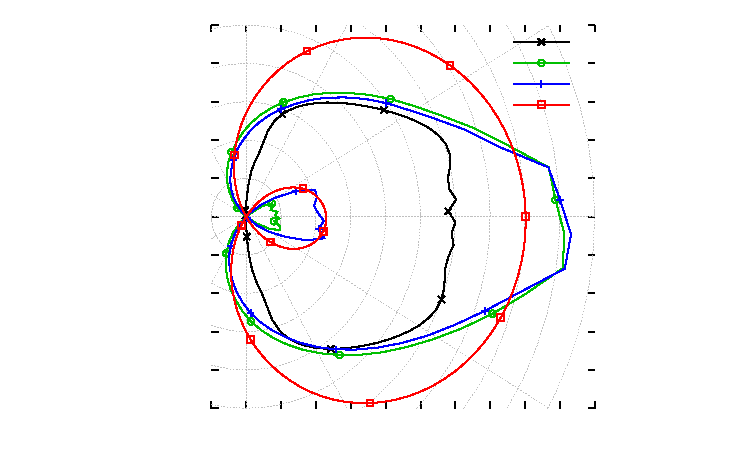
\includegraphics{/Users/seth/_thesis/figures/crashpipe2b/intens-x1-t1/intensity-x1-t1.pdf}}%
    \gplfronttext
  \end{picture}%
\endgroup
}%
  \subfloat[$\psi(1.55,5,\omega)$]{%
    \hspace{-.25in}%
    % GNUPLOT: LaTeX picture with Postscript
\begingroup
  \makeatletter
  \providecommand\color[2][]{%
    \GenericError{(gnuplot) \space\space\space\@spaces}{%
      Package color not loaded in conjunction with
      terminal option `colourtext'%
    }{See the gnuplot documentation for explanation.%
    }{Either use 'blacktext' in gnuplot or load the package
      color.sty in LaTeX.}%
    \renewcommand\color[2][]{}%
  }%
  \providecommand\includegraphics[2][]{%
    \GenericError{(gnuplot) \space\space\space\@spaces}{%
      Package graphicx or graphics not loaded%
    }{See the gnuplot documentation for explanation.%
    }{The gnuplot epslatex terminal needs graphicx.sty or graphics.sty.}%
    \renewcommand\includegraphics[2][]{}%
  }%
  \providecommand\rotatebox[2]{#2}%
  \@ifundefined{ifGPcolor}{%
    \newif\ifGPcolor
    \GPcolortrue
  }{}%
  \@ifundefined{ifGPblacktext}{%
    \newif\ifGPblacktext
    \GPblacktexttrue
  }{}%
  % define a \g@addto@macro without @ in the name:
  \let\gplgaddtomacro\g@addto@macro
  % define empty templates for all commands taking text:
  \gdef\gplbacktext{}%
  \gdef\gplfronttext{}%
  \makeatother
  \ifGPblacktext
    % no textcolor at all
    \def\colorrgb#1{}%
    \def\colorgray#1{}%
  \else
    % gray or color?
    \ifGPcolor
      \def\colorrgb#1{\color[rgb]{#1}}%
      \def\colorgray#1{\color[gray]{#1}}%
      \expandafter\def\csname LTw\endcsname{\color{white}}%
      \expandafter\def\csname LTb\endcsname{\color{black}}%
      \expandafter\def\csname LTa\endcsname{\color{black}}%
      \expandafter\def\csname LT0\endcsname{\color[rgb]{1,0,0}}%
      \expandafter\def\csname LT1\endcsname{\color[rgb]{0,1,0}}%
      \expandafter\def\csname LT2\endcsname{\color[rgb]{0,0,1}}%
      \expandafter\def\csname LT3\endcsname{\color[rgb]{1,0,1}}%
      \expandafter\def\csname LT4\endcsname{\color[rgb]{0,1,1}}%
      \expandafter\def\csname LT5\endcsname{\color[rgb]{1,1,0}}%
      \expandafter\def\csname LT6\endcsname{\color[rgb]{0,0,0}}%
      \expandafter\def\csname LT7\endcsname{\color[rgb]{1,0.3,0}}%
      \expandafter\def\csname LT8\endcsname{\color[rgb]{0.5,0.5,0.5}}%
    \else
      % gray
      \def\colorrgb#1{\color{black}}%
      \def\colorgray#1{\color[gray]{#1}}%
      \expandafter\def\csname LTw\endcsname{\color{white}}%
      \expandafter\def\csname LTb\endcsname{\color{black}}%
      \expandafter\def\csname LTa\endcsname{\color{black}}%
      \expandafter\def\csname LT0\endcsname{\color{black}}%
      \expandafter\def\csname LT1\endcsname{\color{black}}%
      \expandafter\def\csname LT2\endcsname{\color{black}}%
      \expandafter\def\csname LT3\endcsname{\color{black}}%
      \expandafter\def\csname LT4\endcsname{\color{black}}%
      \expandafter\def\csname LT5\endcsname{\color{black}}%
      \expandafter\def\csname LT6\endcsname{\color{black}}%
      \expandafter\def\csname LT7\endcsname{\color{black}}%
      \expandafter\def\csname LT8\endcsname{\color{black}}%
    \fi
  \fi
  \setlength{\unitlength}{0.0500bp}%
  \begin{picture}(7200.00,4320.00)%
    \gplgaddtomacro\gplbacktext{%
      \csname LTb\endcsname%
      \put(1910,400){\makebox(0,0)[r]{\strut{} 0.1}}%
      \put(1910,768){\makebox(0,0)[r]{\strut{} 0.08}}%
      \put(1910,1136){\makebox(0,0)[r]{\strut{} 0.06}}%
      \put(1910,1504){\makebox(0,0)[r]{\strut{} 0.04}}%
      \put(1910,1872){\makebox(0,0)[r]{\strut{} 0.02}}%
      \put(1910,2240){\makebox(0,0)[r]{\strut{} 0}}%
      \put(1910,2607){\makebox(0,0)[r]{\strut{} 0.02}}%
      \put(1910,2975){\makebox(0,0)[r]{\strut{} 0.04}}%
      \put(1910,3343){\makebox(0,0)[r]{\strut{} 0.06}}%
      \put(1910,3711){\makebox(0,0)[r]{\strut{} 0.08}}%
      \put(1910,4079){\makebox(0,0)[r]{\strut{} 0.1}}%
      \csname LTb\endcsname%
      \put(2030,200){\makebox(0,0){\strut{} 0.02}}%
      \csname LTb\endcsname%
      \put(2364,200){\makebox(0,0){\strut{} 0}}%
      \csname LTb\endcsname%
      \put(2699,200){\makebox(0,0){\strut{} 0.02}}%
      \csname LTb\endcsname%
      \put(3033,200){\makebox(0,0){\strut{} 0.04}}%
      \csname LTb\endcsname%
      \put(3368,200){\makebox(0,0){\strut{} 0.06}}%
      \csname LTb\endcsname%
      \put(3702,200){\makebox(0,0){\strut{} 0.08}}%
      \csname LTb\endcsname%
      \put(4037,200){\makebox(0,0){\strut{} 0.1}}%
      \csname LTb\endcsname%
      \put(4371,200){\makebox(0,0){\strut{} 0.12}}%
      \csname LTb\endcsname%
      \put(4706,200){\makebox(0,0){\strut{} 0.14}}%
      \csname LTb\endcsname%
      \put(5040,200){\makebox(0,0){\strut{} 0.16}}%
      \csname LTb\endcsname%
      \put(5375,200){\makebox(0,0){\strut{} 0.18}}%
      \csname LTb\endcsname%
      \put(5709,200){\makebox(0,0){\strut{} 0.2}}%
      \csname LTb\endcsname%
      \put(1330,2239){\rotatebox{-270}{\makebox(0,0){\strut{}x1 center $(1.01,3.5)$}}}%
    }%
    \gplgaddtomacro\gplfronttext{%
      \csname LTb\endcsname%
      \put(4806,3916){\makebox(0,0)[r]{\strut{}S$_{128}$}}%
      \csname LTb\endcsname%
      \put(4806,3716){\makebox(0,0)[r]{\strut{}FLAD$_{64}$}}%
      \csname LTb\endcsname%
      \put(4806,3516){\makebox(0,0)[r]{\strut{}AD$_{64}$}}%
      \csname LTb\endcsname%
      \put(4806,3316){\makebox(0,0)[r]{\strut{}FLD}}%
    }%
    \gplbacktext
    \put(0,0){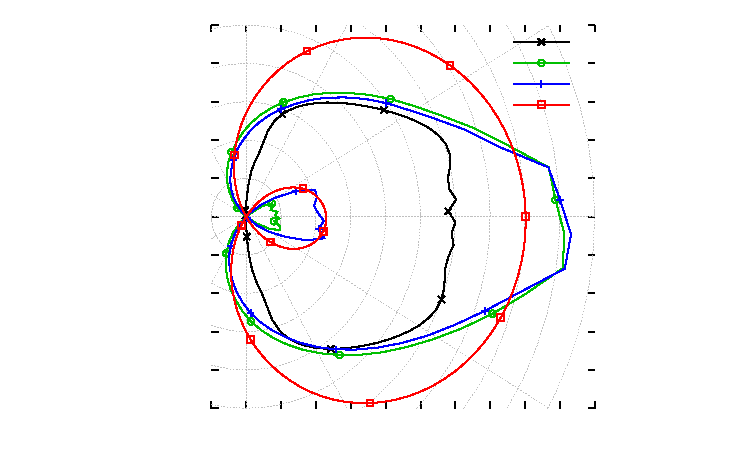
\includegraphics{/Users/seth/_thesis/figures/crashpipe2b/intens-x1-t1/intensity-x1-t1.pdf}}%
    \gplfronttext
  \end{picture}%
\endgroup
}%
  \caption{Angular flux in the channel at (a) the bottom center, (b) the top
  center, and (c) the middle left edge.}
  \label{fig:bcReactorAngular}
\end{figure}

%%%%%%%%%%%%%%%%%%%%%%%%%%%%%%%%%%%%%%%%%%%%%%%%%%%%%%%%%%%%%%%%%%%%%%%%%%%%%%%%
\subsection{Boundary source}

The problems with an incident particle flux on the boundary potentially have
strong gradients and anisotropy outside the applicable range of the anisotropic
diffusion approximation. As an alternative test of the boundary conditions, we
consider three boundary source--driven problems.

\subsubsection{Problem description}

This test problem has opacities identical to the previous problem: two diffusive
regions surround an optically thin channel. However, rather than being driven
by an extraneous source, the problem has an incident radiation flux on the
bottom face. The top, left, and right sides are reflecting. We consider the same
incident angular distributions as in \S\ref{sec:nrFlatlandBcs}, given in
Table~\ref{tab:angularDistributions}: an isotropic
source, a normally-incident source, and a grazing source.

\subsubsection{Results and Discussion}

Figure~\ref{fig:adbcIsotropic} shows a line-out of the scalar flux $\phi(2.5,y)$
along the center of the channel in the isotropic incident case. Standard
diffusion fails because $\sigma=0.01$ leads to a
large diffusion coefficient, resulting in a nearly constant solution inside the
channel. Anisotropic diffusion performs quite well, and the
white boundary condition for $f$ gives a more accurate result than the
reflecting boundary condition.

\begin{figure}[htb]
  \centering
  \centering\small
  \hspace{-.25in}%
  % GNUPLOT: LaTeX picture with Postscript
\begingroup
  \makeatletter
  \providecommand\color[2][]{%
    \GenericError{(gnuplot) \space\space\space\@spaces}{%
      Package color not loaded in conjunction with
      terminal option `colourtext'%
    }{See the gnuplot documentation for explanation.%
    }{Either use 'blacktext' in gnuplot or load the package
      color.sty in LaTeX.}%
    \renewcommand\color[2][]{}%
  }%
  \providecommand\includegraphics[2][]{%
    \GenericError{(gnuplot) \space\space\space\@spaces}{%
      Package graphicx or graphics not loaded%
    }{See the gnuplot documentation for explanation.%
    }{The gnuplot epslatex terminal needs graphicx.sty or graphics.sty.}%
    \renewcommand\includegraphics[2][]{}%
  }%
  \providecommand\rotatebox[2]{#2}%
  \@ifundefined{ifGPcolor}{%
    \newif\ifGPcolor
    \GPcolortrue
  }{}%
  \@ifundefined{ifGPblacktext}{%
    \newif\ifGPblacktext
    \GPblacktexttrue
  }{}%
  % define a \g@addto@macro without @ in the name:
  \let\gplgaddtomacro\g@addto@macro
  % define empty templates for all commands taking text:
  \gdef\gplbacktext{}%
  \gdef\gplfronttext{}%
  \makeatother
  \ifGPblacktext
    % no textcolor at all
    \def\colorrgb#1{}%
    \def\colorgray#1{}%
  \else
    % gray or color?
    \ifGPcolor
      \def\colorrgb#1{\color[rgb]{#1}}%
      \def\colorgray#1{\color[gray]{#1}}%
      \expandafter\def\csname LTw\endcsname{\color{white}}%
      \expandafter\def\csname LTb\endcsname{\color{black}}%
      \expandafter\def\csname LTa\endcsname{\color{black}}%
      \expandafter\def\csname LT0\endcsname{\color[rgb]{1,0,0}}%
      \expandafter\def\csname LT1\endcsname{\color[rgb]{0,1,0}}%
      \expandafter\def\csname LT2\endcsname{\color[rgb]{0,0,1}}%
      \expandafter\def\csname LT3\endcsname{\color[rgb]{1,0,1}}%
      \expandafter\def\csname LT4\endcsname{\color[rgb]{0,1,1}}%
      \expandafter\def\csname LT5\endcsname{\color[rgb]{1,1,0}}%
      \expandafter\def\csname LT6\endcsname{\color[rgb]{0,0,0}}%
      \expandafter\def\csname LT7\endcsname{\color[rgb]{1,0.3,0}}%
      \expandafter\def\csname LT8\endcsname{\color[rgb]{0.5,0.5,0.5}}%
    \else
      % gray
      \def\colorrgb#1{\color{black}}%
      \def\colorgray#1{\color[gray]{#1}}%
      \expandafter\def\csname LTw\endcsname{\color{white}}%
      \expandafter\def\csname LTb\endcsname{\color{black}}%
      \expandafter\def\csname LTa\endcsname{\color{black}}%
      \expandafter\def\csname LT0\endcsname{\color{black}}%
      \expandafter\def\csname LT1\endcsname{\color{black}}%
      \expandafter\def\csname LT2\endcsname{\color{black}}%
      \expandafter\def\csname LT3\endcsname{\color{black}}%
      \expandafter\def\csname LT4\endcsname{\color{black}}%
      \expandafter\def\csname LT5\endcsname{\color{black}}%
      \expandafter\def\csname LT6\endcsname{\color{black}}%
      \expandafter\def\csname LT7\endcsname{\color{black}}%
      \expandafter\def\csname LT8\endcsname{\color{black}}%
    \fi
  \fi
  \setlength{\unitlength}{0.0500bp}%
  \begin{picture}(7200.00,4320.00)%
    \gplgaddtomacro\gplbacktext{%
      \csname LTb\endcsname%
      \put(1910,400){\makebox(0,0)[r]{\strut{} 0.1}}%
      \put(1910,768){\makebox(0,0)[r]{\strut{} 0.08}}%
      \put(1910,1136){\makebox(0,0)[r]{\strut{} 0.06}}%
      \put(1910,1504){\makebox(0,0)[r]{\strut{} 0.04}}%
      \put(1910,1872){\makebox(0,0)[r]{\strut{} 0.02}}%
      \put(1910,2240){\makebox(0,0)[r]{\strut{} 0}}%
      \put(1910,2607){\makebox(0,0)[r]{\strut{} 0.02}}%
      \put(1910,2975){\makebox(0,0)[r]{\strut{} 0.04}}%
      \put(1910,3343){\makebox(0,0)[r]{\strut{} 0.06}}%
      \put(1910,3711){\makebox(0,0)[r]{\strut{} 0.08}}%
      \put(1910,4079){\makebox(0,0)[r]{\strut{} 0.1}}%
      \csname LTb\endcsname%
      \put(2030,200){\makebox(0,0){\strut{} 0.02}}%
      \csname LTb\endcsname%
      \put(2364,200){\makebox(0,0){\strut{} 0}}%
      \csname LTb\endcsname%
      \put(2699,200){\makebox(0,0){\strut{} 0.02}}%
      \csname LTb\endcsname%
      \put(3033,200){\makebox(0,0){\strut{} 0.04}}%
      \csname LTb\endcsname%
      \put(3368,200){\makebox(0,0){\strut{} 0.06}}%
      \csname LTb\endcsname%
      \put(3702,200){\makebox(0,0){\strut{} 0.08}}%
      \csname LTb\endcsname%
      \put(4037,200){\makebox(0,0){\strut{} 0.1}}%
      \csname LTb\endcsname%
      \put(4371,200){\makebox(0,0){\strut{} 0.12}}%
      \csname LTb\endcsname%
      \put(4706,200){\makebox(0,0){\strut{} 0.14}}%
      \csname LTb\endcsname%
      \put(5040,200){\makebox(0,0){\strut{} 0.16}}%
      \csname LTb\endcsname%
      \put(5375,200){\makebox(0,0){\strut{} 0.18}}%
      \csname LTb\endcsname%
      \put(5709,200){\makebox(0,0){\strut{} 0.2}}%
      \csname LTb\endcsname%
      \put(1330,2239){\rotatebox{-270}{\makebox(0,0){\strut{}x1 center $(1.01,3.5)$}}}%
    }%
    \gplgaddtomacro\gplfronttext{%
      \csname LTb\endcsname%
      \put(4806,3916){\makebox(0,0)[r]{\strut{}S$_{128}$}}%
      \csname LTb\endcsname%
      \put(4806,3716){\makebox(0,0)[r]{\strut{}FLAD$_{64}$}}%
      \csname LTb\endcsname%
      \put(4806,3516){\makebox(0,0)[r]{\strut{}AD$_{64}$}}%
      \csname LTb\endcsname%
      \put(4806,3316){\makebox(0,0)[r]{\strut{}FLD}}%
    }%
    \gplbacktext
    \put(0,0){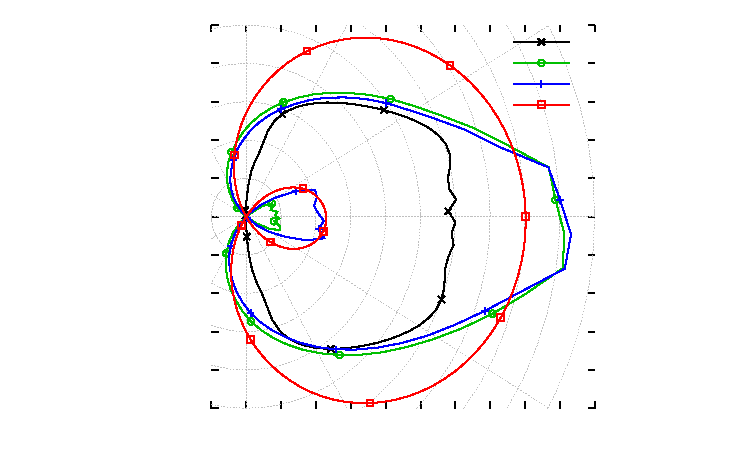
\includegraphics{/Users/seth/_thesis/figures/crashpipe2b/intens-x1-t1/intensity-x1-t1.pdf}}%
    \gplfronttext
  \end{picture}%
\endgroup

  \caption{Scalar flux along the centerline of the channel with an isotropic
  boundary condition at $y=0$.}
  \label{fig:adbcIsotropic}
\end{figure}

The AD approximation and its boundary conditions do have their limits. In the
case of a strongly anisotropic boundary source, the ansatz that
$\vec{F} = O(\epsilon)$ is violated in swaths of the problem, so the solutions
for the normal and grazing boundary conditions have large errors
(Fig.~\ref{fig:adbcRelErr}).

\begin{figure}[htb]
  \centering
  \centering\small
  \hspace{-.25in}%
  % GNUPLOT: LaTeX picture with Postscript
\begingroup
  \makeatletter
  \providecommand\color[2][]{%
    \GenericError{(gnuplot) \space\space\space\@spaces}{%
      Package color not loaded in conjunction with
      terminal option `colourtext'%
    }{See the gnuplot documentation for explanation.%
    }{Either use 'blacktext' in gnuplot or load the package
      color.sty in LaTeX.}%
    \renewcommand\color[2][]{}%
  }%
  \providecommand\includegraphics[2][]{%
    \GenericError{(gnuplot) \space\space\space\@spaces}{%
      Package graphicx or graphics not loaded%
    }{See the gnuplot documentation for explanation.%
    }{The gnuplot epslatex terminal needs graphicx.sty or graphics.sty.}%
    \renewcommand\includegraphics[2][]{}%
  }%
  \providecommand\rotatebox[2]{#2}%
  \@ifundefined{ifGPcolor}{%
    \newif\ifGPcolor
    \GPcolortrue
  }{}%
  \@ifundefined{ifGPblacktext}{%
    \newif\ifGPblacktext
    \GPblacktexttrue
  }{}%
  % define a \g@addto@macro without @ in the name:
  \let\gplgaddtomacro\g@addto@macro
  % define empty templates for all commands taking text:
  \gdef\gplbacktext{}%
  \gdef\gplfronttext{}%
  \makeatother
  \ifGPblacktext
    % no textcolor at all
    \def\colorrgb#1{}%
    \def\colorgray#1{}%
  \else
    % gray or color?
    \ifGPcolor
      \def\colorrgb#1{\color[rgb]{#1}}%
      \def\colorgray#1{\color[gray]{#1}}%
      \expandafter\def\csname LTw\endcsname{\color{white}}%
      \expandafter\def\csname LTb\endcsname{\color{black}}%
      \expandafter\def\csname LTa\endcsname{\color{black}}%
      \expandafter\def\csname LT0\endcsname{\color[rgb]{1,0,0}}%
      \expandafter\def\csname LT1\endcsname{\color[rgb]{0,1,0}}%
      \expandafter\def\csname LT2\endcsname{\color[rgb]{0,0,1}}%
      \expandafter\def\csname LT3\endcsname{\color[rgb]{1,0,1}}%
      \expandafter\def\csname LT4\endcsname{\color[rgb]{0,1,1}}%
      \expandafter\def\csname LT5\endcsname{\color[rgb]{1,1,0}}%
      \expandafter\def\csname LT6\endcsname{\color[rgb]{0,0,0}}%
      \expandafter\def\csname LT7\endcsname{\color[rgb]{1,0.3,0}}%
      \expandafter\def\csname LT8\endcsname{\color[rgb]{0.5,0.5,0.5}}%
    \else
      % gray
      \def\colorrgb#1{\color{black}}%
      \def\colorgray#1{\color[gray]{#1}}%
      \expandafter\def\csname LTw\endcsname{\color{white}}%
      \expandafter\def\csname LTb\endcsname{\color{black}}%
      \expandafter\def\csname LTa\endcsname{\color{black}}%
      \expandafter\def\csname LT0\endcsname{\color{black}}%
      \expandafter\def\csname LT1\endcsname{\color{black}}%
      \expandafter\def\csname LT2\endcsname{\color{black}}%
      \expandafter\def\csname LT3\endcsname{\color{black}}%
      \expandafter\def\csname LT4\endcsname{\color{black}}%
      \expandafter\def\csname LT5\endcsname{\color{black}}%
      \expandafter\def\csname LT6\endcsname{\color{black}}%
      \expandafter\def\csname LT7\endcsname{\color{black}}%
      \expandafter\def\csname LT8\endcsname{\color{black}}%
    \fi
  \fi
  \setlength{\unitlength}{0.0500bp}%
  \begin{picture}(7200.00,4320.00)%
    \gplgaddtomacro\gplbacktext{%
      \csname LTb\endcsname%
      \put(1910,400){\makebox(0,0)[r]{\strut{} 0.1}}%
      \put(1910,768){\makebox(0,0)[r]{\strut{} 0.08}}%
      \put(1910,1136){\makebox(0,0)[r]{\strut{} 0.06}}%
      \put(1910,1504){\makebox(0,0)[r]{\strut{} 0.04}}%
      \put(1910,1872){\makebox(0,0)[r]{\strut{} 0.02}}%
      \put(1910,2240){\makebox(0,0)[r]{\strut{} 0}}%
      \put(1910,2607){\makebox(0,0)[r]{\strut{} 0.02}}%
      \put(1910,2975){\makebox(0,0)[r]{\strut{} 0.04}}%
      \put(1910,3343){\makebox(0,0)[r]{\strut{} 0.06}}%
      \put(1910,3711){\makebox(0,0)[r]{\strut{} 0.08}}%
      \put(1910,4079){\makebox(0,0)[r]{\strut{} 0.1}}%
      \csname LTb\endcsname%
      \put(2030,200){\makebox(0,0){\strut{} 0.02}}%
      \csname LTb\endcsname%
      \put(2364,200){\makebox(0,0){\strut{} 0}}%
      \csname LTb\endcsname%
      \put(2699,200){\makebox(0,0){\strut{} 0.02}}%
      \csname LTb\endcsname%
      \put(3033,200){\makebox(0,0){\strut{} 0.04}}%
      \csname LTb\endcsname%
      \put(3368,200){\makebox(0,0){\strut{} 0.06}}%
      \csname LTb\endcsname%
      \put(3702,200){\makebox(0,0){\strut{} 0.08}}%
      \csname LTb\endcsname%
      \put(4037,200){\makebox(0,0){\strut{} 0.1}}%
      \csname LTb\endcsname%
      \put(4371,200){\makebox(0,0){\strut{} 0.12}}%
      \csname LTb\endcsname%
      \put(4706,200){\makebox(0,0){\strut{} 0.14}}%
      \csname LTb\endcsname%
      \put(5040,200){\makebox(0,0){\strut{} 0.16}}%
      \csname LTb\endcsname%
      \put(5375,200){\makebox(0,0){\strut{} 0.18}}%
      \csname LTb\endcsname%
      \put(5709,200){\makebox(0,0){\strut{} 0.2}}%
      \csname LTb\endcsname%
      \put(1330,2239){\rotatebox{-270}{\makebox(0,0){\strut{}x1 center $(1.01,3.5)$}}}%
    }%
    \gplgaddtomacro\gplfronttext{%
      \csname LTb\endcsname%
      \put(4806,3916){\makebox(0,0)[r]{\strut{}S$_{128}$}}%
      \csname LTb\endcsname%
      \put(4806,3716){\makebox(0,0)[r]{\strut{}FLAD$_{64}$}}%
      \csname LTb\endcsname%
      \put(4806,3516){\makebox(0,0)[r]{\strut{}AD$_{64}$}}%
      \csname LTb\endcsname%
      \put(4806,3316){\makebox(0,0)[r]{\strut{}FLD}}%
    }%
    \gplbacktext
    \put(0,0){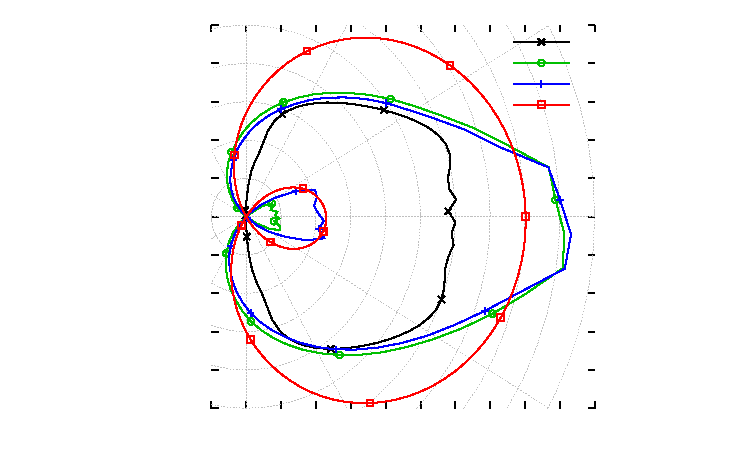
\includegraphics{/Users/seth/_thesis/figures/crashpipe2b/intens-x1-t1/intensity-x1-t1.pdf}}%
    \gplfronttext
  \end{picture}%
\endgroup

  \caption{Relative errors along the centerline of the channel with the three
  different incident boundary conditions.}
  \label{fig:adbcRelErr}
\end{figure}

A visualization of the angular flux for each method (replacing Monte Carlo with
an \SN\ solution), Fig.~\ref{fig:bcChannelIsotropicAngular}, helps explain the
accuracy
of the AD method and the difference between the reflecting and white boundary
treatments. Even though AD cannot exactly model the peak of freely streaming
photons in the channel (which the \SN\ angular flux shows at $\omega=3\pi/2$),
it accurately approximates the angular flux shape driven by scattering from the
diffusive region (the lobes on the left and right) in the isotropic incident
case. In the strongly anisotropic (normal incident source) case, where
uncollided particles from the boundary dominate the scattered particles,
anisotropic diffusion cannot accurately approximate the particle
distribution in the channel.
The linear-in-angle diffusion approximation cannot represent any of these
features.

\begin{figure}[htb]
  \centering\small
  \subfloat[Isotropic]{%
  % GNUPLOT: LaTeX picture with Postscript
\begingroup
  \makeatletter
  \providecommand\color[2][]{%
    \GenericError{(gnuplot) \space\space\space\@spaces}{%
      Package color not loaded in conjunction with
      terminal option `colourtext'%
    }{See the gnuplot documentation for explanation.%
    }{Either use 'blacktext' in gnuplot or load the package
      color.sty in LaTeX.}%
    \renewcommand\color[2][]{}%
  }%
  \providecommand\includegraphics[2][]{%
    \GenericError{(gnuplot) \space\space\space\@spaces}{%
      Package graphicx or graphics not loaded%
    }{See the gnuplot documentation for explanation.%
    }{The gnuplot epslatex terminal needs graphicx.sty or graphics.sty.}%
    \renewcommand\includegraphics[2][]{}%
  }%
  \providecommand\rotatebox[2]{#2}%
  \@ifundefined{ifGPcolor}{%
    \newif\ifGPcolor
    \GPcolortrue
  }{}%
  \@ifundefined{ifGPblacktext}{%
    \newif\ifGPblacktext
    \GPblacktexttrue
  }{}%
  % define a \g@addto@macro without @ in the name:
  \let\gplgaddtomacro\g@addto@macro
  % define empty templates for all commands taking text:
  \gdef\gplbacktext{}%
  \gdef\gplfronttext{}%
  \makeatother
  \ifGPblacktext
    % no textcolor at all
    \def\colorrgb#1{}%
    \def\colorgray#1{}%
  \else
    % gray or color?
    \ifGPcolor
      \def\colorrgb#1{\color[rgb]{#1}}%
      \def\colorgray#1{\color[gray]{#1}}%
      \expandafter\def\csname LTw\endcsname{\color{white}}%
      \expandafter\def\csname LTb\endcsname{\color{black}}%
      \expandafter\def\csname LTa\endcsname{\color{black}}%
      \expandafter\def\csname LT0\endcsname{\color[rgb]{1,0,0}}%
      \expandafter\def\csname LT1\endcsname{\color[rgb]{0,1,0}}%
      \expandafter\def\csname LT2\endcsname{\color[rgb]{0,0,1}}%
      \expandafter\def\csname LT3\endcsname{\color[rgb]{1,0,1}}%
      \expandafter\def\csname LT4\endcsname{\color[rgb]{0,1,1}}%
      \expandafter\def\csname LT5\endcsname{\color[rgb]{1,1,0}}%
      \expandafter\def\csname LT6\endcsname{\color[rgb]{0,0,0}}%
      \expandafter\def\csname LT7\endcsname{\color[rgb]{1,0.3,0}}%
      \expandafter\def\csname LT8\endcsname{\color[rgb]{0.5,0.5,0.5}}%
    \else
      % gray
      \def\colorrgb#1{\color{black}}%
      \def\colorgray#1{\color[gray]{#1}}%
      \expandafter\def\csname LTw\endcsname{\color{white}}%
      \expandafter\def\csname LTb\endcsname{\color{black}}%
      \expandafter\def\csname LTa\endcsname{\color{black}}%
      \expandafter\def\csname LT0\endcsname{\color{black}}%
      \expandafter\def\csname LT1\endcsname{\color{black}}%
      \expandafter\def\csname LT2\endcsname{\color{black}}%
      \expandafter\def\csname LT3\endcsname{\color{black}}%
      \expandafter\def\csname LT4\endcsname{\color{black}}%
      \expandafter\def\csname LT5\endcsname{\color{black}}%
      \expandafter\def\csname LT6\endcsname{\color{black}}%
      \expandafter\def\csname LT7\endcsname{\color{black}}%
      \expandafter\def\csname LT8\endcsname{\color{black}}%
    \fi
  \fi
  \setlength{\unitlength}{0.0500bp}%
  \begin{picture}(7200.00,4320.00)%
    \gplgaddtomacro\gplbacktext{%
      \csname LTb\endcsname%
      \put(1910,400){\makebox(0,0)[r]{\strut{} 0.1}}%
      \put(1910,768){\makebox(0,0)[r]{\strut{} 0.08}}%
      \put(1910,1136){\makebox(0,0)[r]{\strut{} 0.06}}%
      \put(1910,1504){\makebox(0,0)[r]{\strut{} 0.04}}%
      \put(1910,1872){\makebox(0,0)[r]{\strut{} 0.02}}%
      \put(1910,2240){\makebox(0,0)[r]{\strut{} 0}}%
      \put(1910,2607){\makebox(0,0)[r]{\strut{} 0.02}}%
      \put(1910,2975){\makebox(0,0)[r]{\strut{} 0.04}}%
      \put(1910,3343){\makebox(0,0)[r]{\strut{} 0.06}}%
      \put(1910,3711){\makebox(0,0)[r]{\strut{} 0.08}}%
      \put(1910,4079){\makebox(0,0)[r]{\strut{} 0.1}}%
      \csname LTb\endcsname%
      \put(2030,200){\makebox(0,0){\strut{} 0.02}}%
      \csname LTb\endcsname%
      \put(2364,200){\makebox(0,0){\strut{} 0}}%
      \csname LTb\endcsname%
      \put(2699,200){\makebox(0,0){\strut{} 0.02}}%
      \csname LTb\endcsname%
      \put(3033,200){\makebox(0,0){\strut{} 0.04}}%
      \csname LTb\endcsname%
      \put(3368,200){\makebox(0,0){\strut{} 0.06}}%
      \csname LTb\endcsname%
      \put(3702,200){\makebox(0,0){\strut{} 0.08}}%
      \csname LTb\endcsname%
      \put(4037,200){\makebox(0,0){\strut{} 0.1}}%
      \csname LTb\endcsname%
      \put(4371,200){\makebox(0,0){\strut{} 0.12}}%
      \csname LTb\endcsname%
      \put(4706,200){\makebox(0,0){\strut{} 0.14}}%
      \csname LTb\endcsname%
      \put(5040,200){\makebox(0,0){\strut{} 0.16}}%
      \csname LTb\endcsname%
      \put(5375,200){\makebox(0,0){\strut{} 0.18}}%
      \csname LTb\endcsname%
      \put(5709,200){\makebox(0,0){\strut{} 0.2}}%
      \csname LTb\endcsname%
      \put(1330,2239){\rotatebox{-270}{\makebox(0,0){\strut{}x1 center $(1.01,3.5)$}}}%
    }%
    \gplgaddtomacro\gplfronttext{%
      \csname LTb\endcsname%
      \put(4806,3916){\makebox(0,0)[r]{\strut{}S$_{128}$}}%
      \csname LTb\endcsname%
      \put(4806,3716){\makebox(0,0)[r]{\strut{}FLAD$_{64}$}}%
      \csname LTb\endcsname%
      \put(4806,3516){\makebox(0,0)[r]{\strut{}AD$_{64}$}}%
      \csname LTb\endcsname%
      \put(4806,3316){\makebox(0,0)[r]{\strut{}FLD}}%
    }%
    \gplbacktext
    \put(0,0){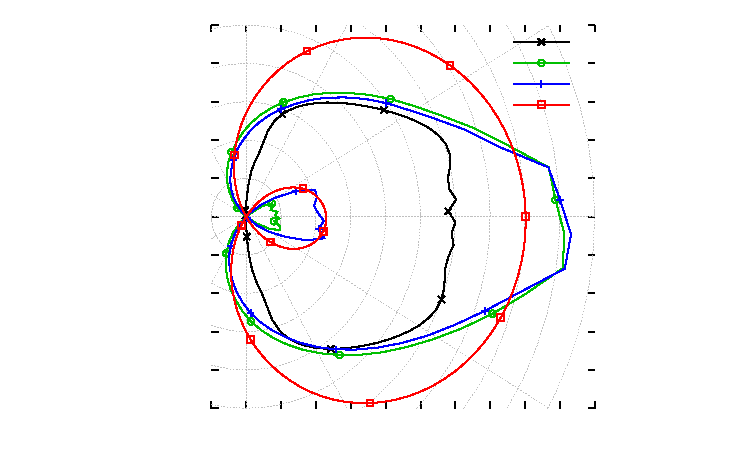
\includegraphics{/Users/seth/_thesis/figures/crashpipe2b/intens-x1-t1/intensity-x1-t1.pdf}}%
    \gplfronttext
  \end{picture}%
\endgroup
%
  \vspace{-.25in}%
  }%
  \subfloat[Normal]{%
  % GNUPLOT: LaTeX picture with Postscript
\begingroup
  \makeatletter
  \providecommand\color[2][]{%
    \GenericError{(gnuplot) \space\space\space\@spaces}{%
      Package color not loaded in conjunction with
      terminal option `colourtext'%
    }{See the gnuplot documentation for explanation.%
    }{Either use 'blacktext' in gnuplot or load the package
      color.sty in LaTeX.}%
    \renewcommand\color[2][]{}%
  }%
  \providecommand\includegraphics[2][]{%
    \GenericError{(gnuplot) \space\space\space\@spaces}{%
      Package graphicx or graphics not loaded%
    }{See the gnuplot documentation for explanation.%
    }{The gnuplot epslatex terminal needs graphicx.sty or graphics.sty.}%
    \renewcommand\includegraphics[2][]{}%
  }%
  \providecommand\rotatebox[2]{#2}%
  \@ifundefined{ifGPcolor}{%
    \newif\ifGPcolor
    \GPcolortrue
  }{}%
  \@ifundefined{ifGPblacktext}{%
    \newif\ifGPblacktext
    \GPblacktexttrue
  }{}%
  % define a \g@addto@macro without @ in the name:
  \let\gplgaddtomacro\g@addto@macro
  % define empty templates for all commands taking text:
  \gdef\gplbacktext{}%
  \gdef\gplfronttext{}%
  \makeatother
  \ifGPblacktext
    % no textcolor at all
    \def\colorrgb#1{}%
    \def\colorgray#1{}%
  \else
    % gray or color?
    \ifGPcolor
      \def\colorrgb#1{\color[rgb]{#1}}%
      \def\colorgray#1{\color[gray]{#1}}%
      \expandafter\def\csname LTw\endcsname{\color{white}}%
      \expandafter\def\csname LTb\endcsname{\color{black}}%
      \expandafter\def\csname LTa\endcsname{\color{black}}%
      \expandafter\def\csname LT0\endcsname{\color[rgb]{1,0,0}}%
      \expandafter\def\csname LT1\endcsname{\color[rgb]{0,1,0}}%
      \expandafter\def\csname LT2\endcsname{\color[rgb]{0,0,1}}%
      \expandafter\def\csname LT3\endcsname{\color[rgb]{1,0,1}}%
      \expandafter\def\csname LT4\endcsname{\color[rgb]{0,1,1}}%
      \expandafter\def\csname LT5\endcsname{\color[rgb]{1,1,0}}%
      \expandafter\def\csname LT6\endcsname{\color[rgb]{0,0,0}}%
      \expandafter\def\csname LT7\endcsname{\color[rgb]{1,0.3,0}}%
      \expandafter\def\csname LT8\endcsname{\color[rgb]{0.5,0.5,0.5}}%
    \else
      % gray
      \def\colorrgb#1{\color{black}}%
      \def\colorgray#1{\color[gray]{#1}}%
      \expandafter\def\csname LTw\endcsname{\color{white}}%
      \expandafter\def\csname LTb\endcsname{\color{black}}%
      \expandafter\def\csname LTa\endcsname{\color{black}}%
      \expandafter\def\csname LT0\endcsname{\color{black}}%
      \expandafter\def\csname LT1\endcsname{\color{black}}%
      \expandafter\def\csname LT2\endcsname{\color{black}}%
      \expandafter\def\csname LT3\endcsname{\color{black}}%
      \expandafter\def\csname LT4\endcsname{\color{black}}%
      \expandafter\def\csname LT5\endcsname{\color{black}}%
      \expandafter\def\csname LT6\endcsname{\color{black}}%
      \expandafter\def\csname LT7\endcsname{\color{black}}%
      \expandafter\def\csname LT8\endcsname{\color{black}}%
    \fi
  \fi
  \setlength{\unitlength}{0.0500bp}%
  \begin{picture}(7200.00,4320.00)%
    \gplgaddtomacro\gplbacktext{%
      \csname LTb\endcsname%
      \put(1910,400){\makebox(0,0)[r]{\strut{} 0.1}}%
      \put(1910,768){\makebox(0,0)[r]{\strut{} 0.08}}%
      \put(1910,1136){\makebox(0,0)[r]{\strut{} 0.06}}%
      \put(1910,1504){\makebox(0,0)[r]{\strut{} 0.04}}%
      \put(1910,1872){\makebox(0,0)[r]{\strut{} 0.02}}%
      \put(1910,2240){\makebox(0,0)[r]{\strut{} 0}}%
      \put(1910,2607){\makebox(0,0)[r]{\strut{} 0.02}}%
      \put(1910,2975){\makebox(0,0)[r]{\strut{} 0.04}}%
      \put(1910,3343){\makebox(0,0)[r]{\strut{} 0.06}}%
      \put(1910,3711){\makebox(0,0)[r]{\strut{} 0.08}}%
      \put(1910,4079){\makebox(0,0)[r]{\strut{} 0.1}}%
      \csname LTb\endcsname%
      \put(2030,200){\makebox(0,0){\strut{} 0.02}}%
      \csname LTb\endcsname%
      \put(2364,200){\makebox(0,0){\strut{} 0}}%
      \csname LTb\endcsname%
      \put(2699,200){\makebox(0,0){\strut{} 0.02}}%
      \csname LTb\endcsname%
      \put(3033,200){\makebox(0,0){\strut{} 0.04}}%
      \csname LTb\endcsname%
      \put(3368,200){\makebox(0,0){\strut{} 0.06}}%
      \csname LTb\endcsname%
      \put(3702,200){\makebox(0,0){\strut{} 0.08}}%
      \csname LTb\endcsname%
      \put(4037,200){\makebox(0,0){\strut{} 0.1}}%
      \csname LTb\endcsname%
      \put(4371,200){\makebox(0,0){\strut{} 0.12}}%
      \csname LTb\endcsname%
      \put(4706,200){\makebox(0,0){\strut{} 0.14}}%
      \csname LTb\endcsname%
      \put(5040,200){\makebox(0,0){\strut{} 0.16}}%
      \csname LTb\endcsname%
      \put(5375,200){\makebox(0,0){\strut{} 0.18}}%
      \csname LTb\endcsname%
      \put(5709,200){\makebox(0,0){\strut{} 0.2}}%
      \csname LTb\endcsname%
      \put(1330,2239){\rotatebox{-270}{\makebox(0,0){\strut{}x1 center $(1.01,3.5)$}}}%
    }%
    \gplgaddtomacro\gplfronttext{%
      \csname LTb\endcsname%
      \put(4806,3916){\makebox(0,0)[r]{\strut{}S$_{128}$}}%
      \csname LTb\endcsname%
      \put(4806,3716){\makebox(0,0)[r]{\strut{}FLAD$_{64}$}}%
      \csname LTb\endcsname%
      \put(4806,3516){\makebox(0,0)[r]{\strut{}AD$_{64}$}}%
      \csname LTb\endcsname%
      \put(4806,3316){\makebox(0,0)[r]{\strut{}FLD}}%
    }%
    \gplbacktext
    \put(0,0){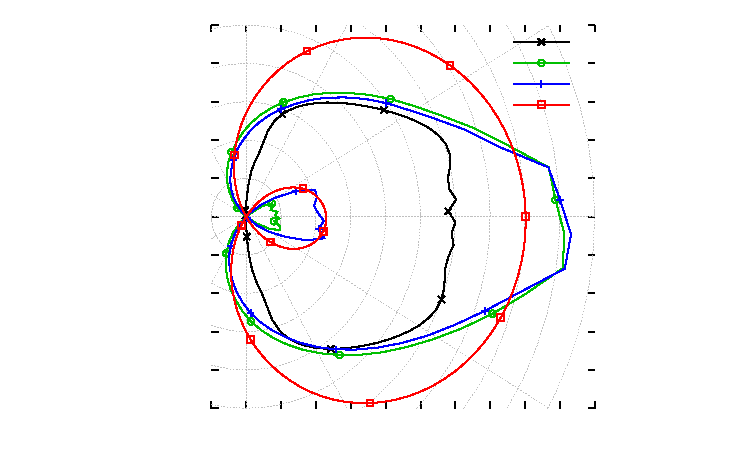
\includegraphics{/Users/seth/_thesis/figures/crashpipe2b/intens-x1-t1/intensity-x1-t1.pdf}}%
    \gplfronttext
  \end{picture}%
\endgroup
%
  \vspace{-.25in}%
  }%
  \Caption{Angular flux $\psi(2.5, 1, \omega)$ in the incident boundary source
  problem.}{
  The isotropic (a) and normal (b) incident cases are plotted in the centerline
  of the channel, one unit from the boundary.}
  \label{fig:bcChannelIsotropicAngular}
\end{figure}

The shape around $\omega=\pi/2$ gives insight into why the white boundary
performs slightly better in the case of an isotropic incident boundary
condition: a reflecting boundary produces a peak in $f$
along the channel, but a white boundary gives a more isotropic shape near that
range, better matching the incident isotropic boundary condition. This suggests
that the qualitatively best way to satisfy Eq.~\eqref{eq:hoBc} may be
to require the incident distribution of $f$ to take the shape of the true
boundary condition.

%%%%%%%%%%%%%%%%%%%%%%%%%%%%%%%%%%%%%%%%%%%%%%%%%%%%%%%%%%%%%%%%%%%%%%%%%%%%%%%%
\section{Smooth time-dependent problem}

One novel extension to the anisotropic diffusion approximation is the
formulation for time-dependent transport. Even though our primary application is
the time-dependent nonlinear thermal radiative transfer, we stress that the
nonlinearities are incidental to the AD approximation. We therefore 
test the behavior of the anisotropic diffusion methods in a more simple
situation: linear, time-dependent problems with time-independent opacities.

In this first time-dependent problem, we expect the temporal and spatial
gradients to be moderate but significant enough to distinguish diffusion from
transport.

\subsection{Problem description}

This smooth problem features a unit source in the bottom left corner of a
highly scattering medium of width~$2$ with
$\sigma=1$ and $\sigma_s=.99$. A voided region with width $0.5$,
$\sigma=0.01$, and $\sigma_s=.0099$ lies along the right edge of the problem.
The bottom,
left, and right boundaries are reflecting; the top of the problem has a vacuum
boundary. The problem's initial condition is uniformly zero, and the particle
speed is unity ($c=1$).

Because this problem is time-dependent, it is the first test of the anisotropic
\Pone\ method devised in Chapter~\ref{chap:aponeDerivation}. This method
uses not only the anisotropic diffusion tensors $\Dtens$ but also a nonlocal
opacity $\varsigma$, as formulated in \eqref{eq:ap1FicksLawFinal}:
\begin{equation*}
  \frac{1}{c}\pder{\vec{F}}{t}(\vec{x},t)
  + \varsigma(\vec{x}) \Dtens(\vec{x}) \vd \grad \phi(\vec{x}, t)
  + \varsigma(\vec{x})\vec{F}(\vec{x},t) 
  = 0 \,.
\end{equation*}
Figure~\ref{fig:tdReactorProblem} overlays these transport-calculated
coefficients on the problem's physical description.

\begin{figure}[htb]
  \centering
  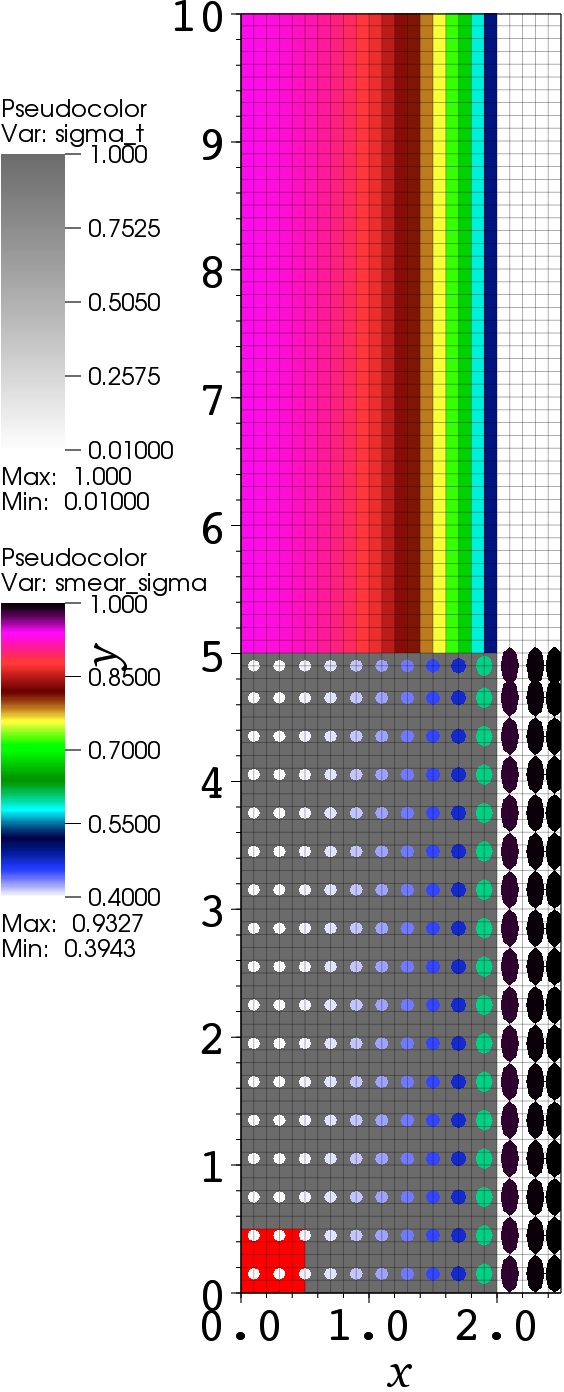
\includegraphics[width=1.25in]{td_reactor/xsn}
  \Caption{Time-dependent smooth problem properties.}{
    The source region is the red square in the lower-left; the black
    and white area in the bottom half shows $\sigma$, the colored region above
    shows $\varsigma = 1/\int_{S} f \ud\Omega$, and the ellipses are a
    visualization of the diffusion tensor $\Dtens=\int_{S}
    \vec{\Omega}\vec{\Omega} f \ud\Omega$.}
  \label{fig:tdReactorProblem}
\end{figure}

In this figure, the anisotropic diffusion tensors are plotted as ellipses. Each
ellipse's major axis
lies along the principal eigenvector of $\Dtens$, and the size along that axis is
proportional to the corresponding eigenvalue. The minor axis is proportional to
the second eigenvalue of the tensor. If $f$ is isotropic, $\Dtens$ is
proportional to the identity tensor, and its two eigenvalues are equal: thus, in
the interior, the anisotropic diffusion coefficients appear as circles whose
sizes are proportional to $1/\sigma$.

\subsection{Results and Discussion}

The large phase space of time-dependent transport forces us to carefully choose
representative metrics. We use contour plots to compare select methods at
select times, lineouts to compare more methods in greater detail, and wavefront
plots to visualize the detailed time evolution of the problem.

The behavior of $\phi$ along the center of the channel (i.e., at the
right edge of the problem) is plotted in Fig.~\ref{fig:tdReactor}. Anisotropic
diffusion and conventional diffusion, which both assume a quasi-static problem,
are significantly less accurate and are not plotted in that figure. Their
more accurate flux-limited counterparts, FLAD and FLD, are shown instead.

\begin{figure}[htb]
  \centering\small
  \subfloat[$t=2$]{%
    \hspace{-.25in}%
    % GNUPLOT: LaTeX picture with Postscript
\begingroup
  \makeatletter
  \providecommand\color[2][]{%
    \GenericError{(gnuplot) \space\space\space\@spaces}{%
      Package color not loaded in conjunction with
      terminal option `colourtext'%
    }{See the gnuplot documentation for explanation.%
    }{Either use 'blacktext' in gnuplot or load the package
      color.sty in LaTeX.}%
    \renewcommand\color[2][]{}%
  }%
  \providecommand\includegraphics[2][]{%
    \GenericError{(gnuplot) \space\space\space\@spaces}{%
      Package graphicx or graphics not loaded%
    }{See the gnuplot documentation for explanation.%
    }{The gnuplot epslatex terminal needs graphicx.sty or graphics.sty.}%
    \renewcommand\includegraphics[2][]{}%
  }%
  \providecommand\rotatebox[2]{#2}%
  \@ifundefined{ifGPcolor}{%
    \newif\ifGPcolor
    \GPcolortrue
  }{}%
  \@ifundefined{ifGPblacktext}{%
    \newif\ifGPblacktext
    \GPblacktexttrue
  }{}%
  % define a \g@addto@macro without @ in the name:
  \let\gplgaddtomacro\g@addto@macro
  % define empty templates for all commands taking text:
  \gdef\gplbacktext{}%
  \gdef\gplfronttext{}%
  \makeatother
  \ifGPblacktext
    % no textcolor at all
    \def\colorrgb#1{}%
    \def\colorgray#1{}%
  \else
    % gray or color?
    \ifGPcolor
      \def\colorrgb#1{\color[rgb]{#1}}%
      \def\colorgray#1{\color[gray]{#1}}%
      \expandafter\def\csname LTw\endcsname{\color{white}}%
      \expandafter\def\csname LTb\endcsname{\color{black}}%
      \expandafter\def\csname LTa\endcsname{\color{black}}%
      \expandafter\def\csname LT0\endcsname{\color[rgb]{1,0,0}}%
      \expandafter\def\csname LT1\endcsname{\color[rgb]{0,1,0}}%
      \expandafter\def\csname LT2\endcsname{\color[rgb]{0,0,1}}%
      \expandafter\def\csname LT3\endcsname{\color[rgb]{1,0,1}}%
      \expandafter\def\csname LT4\endcsname{\color[rgb]{0,1,1}}%
      \expandafter\def\csname LT5\endcsname{\color[rgb]{1,1,0}}%
      \expandafter\def\csname LT6\endcsname{\color[rgb]{0,0,0}}%
      \expandafter\def\csname LT7\endcsname{\color[rgb]{1,0.3,0}}%
      \expandafter\def\csname LT8\endcsname{\color[rgb]{0.5,0.5,0.5}}%
    \else
      % gray
      \def\colorrgb#1{\color{black}}%
      \def\colorgray#1{\color[gray]{#1}}%
      \expandafter\def\csname LTw\endcsname{\color{white}}%
      \expandafter\def\csname LTb\endcsname{\color{black}}%
      \expandafter\def\csname LTa\endcsname{\color{black}}%
      \expandafter\def\csname LT0\endcsname{\color{black}}%
      \expandafter\def\csname LT1\endcsname{\color{black}}%
      \expandafter\def\csname LT2\endcsname{\color{black}}%
      \expandafter\def\csname LT3\endcsname{\color{black}}%
      \expandafter\def\csname LT4\endcsname{\color{black}}%
      \expandafter\def\csname LT5\endcsname{\color{black}}%
      \expandafter\def\csname LT6\endcsname{\color{black}}%
      \expandafter\def\csname LT7\endcsname{\color{black}}%
      \expandafter\def\csname LT8\endcsname{\color{black}}%
    \fi
  \fi
  \setlength{\unitlength}{0.0500bp}%
  \begin{picture}(7200.00,4320.00)%
    \gplgaddtomacro\gplbacktext{%
      \csname LTb\endcsname%
      \put(1910,400){\makebox(0,0)[r]{\strut{} 0.1}}%
      \put(1910,768){\makebox(0,0)[r]{\strut{} 0.08}}%
      \put(1910,1136){\makebox(0,0)[r]{\strut{} 0.06}}%
      \put(1910,1504){\makebox(0,0)[r]{\strut{} 0.04}}%
      \put(1910,1872){\makebox(0,0)[r]{\strut{} 0.02}}%
      \put(1910,2240){\makebox(0,0)[r]{\strut{} 0}}%
      \put(1910,2607){\makebox(0,0)[r]{\strut{} 0.02}}%
      \put(1910,2975){\makebox(0,0)[r]{\strut{} 0.04}}%
      \put(1910,3343){\makebox(0,0)[r]{\strut{} 0.06}}%
      \put(1910,3711){\makebox(0,0)[r]{\strut{} 0.08}}%
      \put(1910,4079){\makebox(0,0)[r]{\strut{} 0.1}}%
      \csname LTb\endcsname%
      \put(2030,200){\makebox(0,0){\strut{} 0.02}}%
      \csname LTb\endcsname%
      \put(2364,200){\makebox(0,0){\strut{} 0}}%
      \csname LTb\endcsname%
      \put(2699,200){\makebox(0,0){\strut{} 0.02}}%
      \csname LTb\endcsname%
      \put(3033,200){\makebox(0,0){\strut{} 0.04}}%
      \csname LTb\endcsname%
      \put(3368,200){\makebox(0,0){\strut{} 0.06}}%
      \csname LTb\endcsname%
      \put(3702,200){\makebox(0,0){\strut{} 0.08}}%
      \csname LTb\endcsname%
      \put(4037,200){\makebox(0,0){\strut{} 0.1}}%
      \csname LTb\endcsname%
      \put(4371,200){\makebox(0,0){\strut{} 0.12}}%
      \csname LTb\endcsname%
      \put(4706,200){\makebox(0,0){\strut{} 0.14}}%
      \csname LTb\endcsname%
      \put(5040,200){\makebox(0,0){\strut{} 0.16}}%
      \csname LTb\endcsname%
      \put(5375,200){\makebox(0,0){\strut{} 0.18}}%
      \csname LTb\endcsname%
      \put(5709,200){\makebox(0,0){\strut{} 0.2}}%
      \csname LTb\endcsname%
      \put(1330,2239){\rotatebox{-270}{\makebox(0,0){\strut{}x1 center $(1.01,3.5)$}}}%
    }%
    \gplgaddtomacro\gplfronttext{%
      \csname LTb\endcsname%
      \put(4806,3916){\makebox(0,0)[r]{\strut{}S$_{128}$}}%
      \csname LTb\endcsname%
      \put(4806,3716){\makebox(0,0)[r]{\strut{}FLAD$_{64}$}}%
      \csname LTb\endcsname%
      \put(4806,3516){\makebox(0,0)[r]{\strut{}AD$_{64}$}}%
      \csname LTb\endcsname%
      \put(4806,3316){\makebox(0,0)[r]{\strut{}FLD}}%
    }%
    \gplbacktext
    \put(0,0){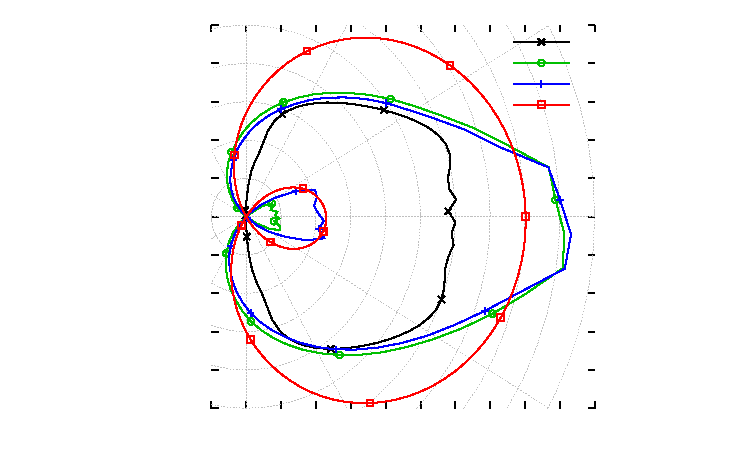
\includegraphics{/Users/seth/_thesis/figures/crashpipe2b/intens-x1-t1/intensity-x1-t1.pdf}}%
    \gplfronttext
  \end{picture}%
\endgroup
}%
  \subfloat[$t=5$]{%
    \hspace{-.25in}%
    % GNUPLOT: LaTeX picture with Postscript
\begingroup
  \makeatletter
  \providecommand\color[2][]{%
    \GenericError{(gnuplot) \space\space\space\@spaces}{%
      Package color not loaded in conjunction with
      terminal option `colourtext'%
    }{See the gnuplot documentation for explanation.%
    }{Either use 'blacktext' in gnuplot or load the package
      color.sty in LaTeX.}%
    \renewcommand\color[2][]{}%
  }%
  \providecommand\includegraphics[2][]{%
    \GenericError{(gnuplot) \space\space\space\@spaces}{%
      Package graphicx or graphics not loaded%
    }{See the gnuplot documentation for explanation.%
    }{The gnuplot epslatex terminal needs graphicx.sty or graphics.sty.}%
    \renewcommand\includegraphics[2][]{}%
  }%
  \providecommand\rotatebox[2]{#2}%
  \@ifundefined{ifGPcolor}{%
    \newif\ifGPcolor
    \GPcolortrue
  }{}%
  \@ifundefined{ifGPblacktext}{%
    \newif\ifGPblacktext
    \GPblacktexttrue
  }{}%
  % define a \g@addto@macro without @ in the name:
  \let\gplgaddtomacro\g@addto@macro
  % define empty templates for all commands taking text:
  \gdef\gplbacktext{}%
  \gdef\gplfronttext{}%
  \makeatother
  \ifGPblacktext
    % no textcolor at all
    \def\colorrgb#1{}%
    \def\colorgray#1{}%
  \else
    % gray or color?
    \ifGPcolor
      \def\colorrgb#1{\color[rgb]{#1}}%
      \def\colorgray#1{\color[gray]{#1}}%
      \expandafter\def\csname LTw\endcsname{\color{white}}%
      \expandafter\def\csname LTb\endcsname{\color{black}}%
      \expandafter\def\csname LTa\endcsname{\color{black}}%
      \expandafter\def\csname LT0\endcsname{\color[rgb]{1,0,0}}%
      \expandafter\def\csname LT1\endcsname{\color[rgb]{0,1,0}}%
      \expandafter\def\csname LT2\endcsname{\color[rgb]{0,0,1}}%
      \expandafter\def\csname LT3\endcsname{\color[rgb]{1,0,1}}%
      \expandafter\def\csname LT4\endcsname{\color[rgb]{0,1,1}}%
      \expandafter\def\csname LT5\endcsname{\color[rgb]{1,1,0}}%
      \expandafter\def\csname LT6\endcsname{\color[rgb]{0,0,0}}%
      \expandafter\def\csname LT7\endcsname{\color[rgb]{1,0.3,0}}%
      \expandafter\def\csname LT8\endcsname{\color[rgb]{0.5,0.5,0.5}}%
    \else
      % gray
      \def\colorrgb#1{\color{black}}%
      \def\colorgray#1{\color[gray]{#1}}%
      \expandafter\def\csname LTw\endcsname{\color{white}}%
      \expandafter\def\csname LTb\endcsname{\color{black}}%
      \expandafter\def\csname LTa\endcsname{\color{black}}%
      \expandafter\def\csname LT0\endcsname{\color{black}}%
      \expandafter\def\csname LT1\endcsname{\color{black}}%
      \expandafter\def\csname LT2\endcsname{\color{black}}%
      \expandafter\def\csname LT3\endcsname{\color{black}}%
      \expandafter\def\csname LT4\endcsname{\color{black}}%
      \expandafter\def\csname LT5\endcsname{\color{black}}%
      \expandafter\def\csname LT6\endcsname{\color{black}}%
      \expandafter\def\csname LT7\endcsname{\color{black}}%
      \expandafter\def\csname LT8\endcsname{\color{black}}%
    \fi
  \fi
  \setlength{\unitlength}{0.0500bp}%
  \begin{picture}(7200.00,4320.00)%
    \gplgaddtomacro\gplbacktext{%
      \csname LTb\endcsname%
      \put(1910,400){\makebox(0,0)[r]{\strut{} 0.1}}%
      \put(1910,768){\makebox(0,0)[r]{\strut{} 0.08}}%
      \put(1910,1136){\makebox(0,0)[r]{\strut{} 0.06}}%
      \put(1910,1504){\makebox(0,0)[r]{\strut{} 0.04}}%
      \put(1910,1872){\makebox(0,0)[r]{\strut{} 0.02}}%
      \put(1910,2240){\makebox(0,0)[r]{\strut{} 0}}%
      \put(1910,2607){\makebox(0,0)[r]{\strut{} 0.02}}%
      \put(1910,2975){\makebox(0,0)[r]{\strut{} 0.04}}%
      \put(1910,3343){\makebox(0,0)[r]{\strut{} 0.06}}%
      \put(1910,3711){\makebox(0,0)[r]{\strut{} 0.08}}%
      \put(1910,4079){\makebox(0,0)[r]{\strut{} 0.1}}%
      \csname LTb\endcsname%
      \put(2030,200){\makebox(0,0){\strut{} 0.02}}%
      \csname LTb\endcsname%
      \put(2364,200){\makebox(0,0){\strut{} 0}}%
      \csname LTb\endcsname%
      \put(2699,200){\makebox(0,0){\strut{} 0.02}}%
      \csname LTb\endcsname%
      \put(3033,200){\makebox(0,0){\strut{} 0.04}}%
      \csname LTb\endcsname%
      \put(3368,200){\makebox(0,0){\strut{} 0.06}}%
      \csname LTb\endcsname%
      \put(3702,200){\makebox(0,0){\strut{} 0.08}}%
      \csname LTb\endcsname%
      \put(4037,200){\makebox(0,0){\strut{} 0.1}}%
      \csname LTb\endcsname%
      \put(4371,200){\makebox(0,0){\strut{} 0.12}}%
      \csname LTb\endcsname%
      \put(4706,200){\makebox(0,0){\strut{} 0.14}}%
      \csname LTb\endcsname%
      \put(5040,200){\makebox(0,0){\strut{} 0.16}}%
      \csname LTb\endcsname%
      \put(5375,200){\makebox(0,0){\strut{} 0.18}}%
      \csname LTb\endcsname%
      \put(5709,200){\makebox(0,0){\strut{} 0.2}}%
      \csname LTb\endcsname%
      \put(1330,2239){\rotatebox{-270}{\makebox(0,0){\strut{}x1 center $(1.01,3.5)$}}}%
    }%
    \gplgaddtomacro\gplfronttext{%
      \csname LTb\endcsname%
      \put(4806,3916){\makebox(0,0)[r]{\strut{}S$_{128}$}}%
      \csname LTb\endcsname%
      \put(4806,3716){\makebox(0,0)[r]{\strut{}FLAD$_{64}$}}%
      \csname LTb\endcsname%
      \put(4806,3516){\makebox(0,0)[r]{\strut{}AD$_{64}$}}%
      \csname LTb\endcsname%
      \put(4806,3316){\makebox(0,0)[r]{\strut{}FLD}}%
    }%
    \gplbacktext
    \put(0,0){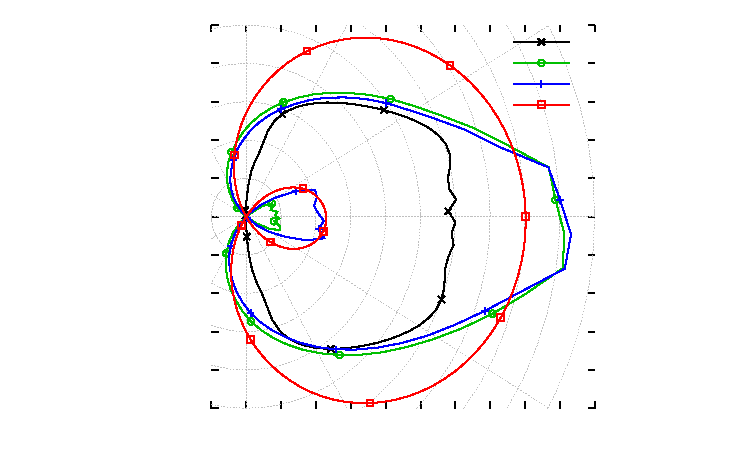
\includegraphics{/Users/seth/_thesis/figures/crashpipe2b/intens-x1-t1/intensity-x1-t1.pdf}}%
    \gplfronttext
  \end{picture}%
\endgroup
}

  \subfloat[$t=10$]{%
    \hspace{-.25in}%
    % GNUPLOT: LaTeX picture with Postscript
\begingroup
  \makeatletter
  \providecommand\color[2][]{%
    \GenericError{(gnuplot) \space\space\space\@spaces}{%
      Package color not loaded in conjunction with
      terminal option `colourtext'%
    }{See the gnuplot documentation for explanation.%
    }{Either use 'blacktext' in gnuplot or load the package
      color.sty in LaTeX.}%
    \renewcommand\color[2][]{}%
  }%
  \providecommand\includegraphics[2][]{%
    \GenericError{(gnuplot) \space\space\space\@spaces}{%
      Package graphicx or graphics not loaded%
    }{See the gnuplot documentation for explanation.%
    }{The gnuplot epslatex terminal needs graphicx.sty or graphics.sty.}%
    \renewcommand\includegraphics[2][]{}%
  }%
  \providecommand\rotatebox[2]{#2}%
  \@ifundefined{ifGPcolor}{%
    \newif\ifGPcolor
    \GPcolortrue
  }{}%
  \@ifundefined{ifGPblacktext}{%
    \newif\ifGPblacktext
    \GPblacktexttrue
  }{}%
  % define a \g@addto@macro without @ in the name:
  \let\gplgaddtomacro\g@addto@macro
  % define empty templates for all commands taking text:
  \gdef\gplbacktext{}%
  \gdef\gplfronttext{}%
  \makeatother
  \ifGPblacktext
    % no textcolor at all
    \def\colorrgb#1{}%
    \def\colorgray#1{}%
  \else
    % gray or color?
    \ifGPcolor
      \def\colorrgb#1{\color[rgb]{#1}}%
      \def\colorgray#1{\color[gray]{#1}}%
      \expandafter\def\csname LTw\endcsname{\color{white}}%
      \expandafter\def\csname LTb\endcsname{\color{black}}%
      \expandafter\def\csname LTa\endcsname{\color{black}}%
      \expandafter\def\csname LT0\endcsname{\color[rgb]{1,0,0}}%
      \expandafter\def\csname LT1\endcsname{\color[rgb]{0,1,0}}%
      \expandafter\def\csname LT2\endcsname{\color[rgb]{0,0,1}}%
      \expandafter\def\csname LT3\endcsname{\color[rgb]{1,0,1}}%
      \expandafter\def\csname LT4\endcsname{\color[rgb]{0,1,1}}%
      \expandafter\def\csname LT5\endcsname{\color[rgb]{1,1,0}}%
      \expandafter\def\csname LT6\endcsname{\color[rgb]{0,0,0}}%
      \expandafter\def\csname LT7\endcsname{\color[rgb]{1,0.3,0}}%
      \expandafter\def\csname LT8\endcsname{\color[rgb]{0.5,0.5,0.5}}%
    \else
      % gray
      \def\colorrgb#1{\color{black}}%
      \def\colorgray#1{\color[gray]{#1}}%
      \expandafter\def\csname LTw\endcsname{\color{white}}%
      \expandafter\def\csname LTb\endcsname{\color{black}}%
      \expandafter\def\csname LTa\endcsname{\color{black}}%
      \expandafter\def\csname LT0\endcsname{\color{black}}%
      \expandafter\def\csname LT1\endcsname{\color{black}}%
      \expandafter\def\csname LT2\endcsname{\color{black}}%
      \expandafter\def\csname LT3\endcsname{\color{black}}%
      \expandafter\def\csname LT4\endcsname{\color{black}}%
      \expandafter\def\csname LT5\endcsname{\color{black}}%
      \expandafter\def\csname LT6\endcsname{\color{black}}%
      \expandafter\def\csname LT7\endcsname{\color{black}}%
      \expandafter\def\csname LT8\endcsname{\color{black}}%
    \fi
  \fi
  \setlength{\unitlength}{0.0500bp}%
  \begin{picture}(7200.00,4320.00)%
    \gplgaddtomacro\gplbacktext{%
      \csname LTb\endcsname%
      \put(1910,400){\makebox(0,0)[r]{\strut{} 0.1}}%
      \put(1910,768){\makebox(0,0)[r]{\strut{} 0.08}}%
      \put(1910,1136){\makebox(0,0)[r]{\strut{} 0.06}}%
      \put(1910,1504){\makebox(0,0)[r]{\strut{} 0.04}}%
      \put(1910,1872){\makebox(0,0)[r]{\strut{} 0.02}}%
      \put(1910,2240){\makebox(0,0)[r]{\strut{} 0}}%
      \put(1910,2607){\makebox(0,0)[r]{\strut{} 0.02}}%
      \put(1910,2975){\makebox(0,0)[r]{\strut{} 0.04}}%
      \put(1910,3343){\makebox(0,0)[r]{\strut{} 0.06}}%
      \put(1910,3711){\makebox(0,0)[r]{\strut{} 0.08}}%
      \put(1910,4079){\makebox(0,0)[r]{\strut{} 0.1}}%
      \csname LTb\endcsname%
      \put(2030,200){\makebox(0,0){\strut{} 0.02}}%
      \csname LTb\endcsname%
      \put(2364,200){\makebox(0,0){\strut{} 0}}%
      \csname LTb\endcsname%
      \put(2699,200){\makebox(0,0){\strut{} 0.02}}%
      \csname LTb\endcsname%
      \put(3033,200){\makebox(0,0){\strut{} 0.04}}%
      \csname LTb\endcsname%
      \put(3368,200){\makebox(0,0){\strut{} 0.06}}%
      \csname LTb\endcsname%
      \put(3702,200){\makebox(0,0){\strut{} 0.08}}%
      \csname LTb\endcsname%
      \put(4037,200){\makebox(0,0){\strut{} 0.1}}%
      \csname LTb\endcsname%
      \put(4371,200){\makebox(0,0){\strut{} 0.12}}%
      \csname LTb\endcsname%
      \put(4706,200){\makebox(0,0){\strut{} 0.14}}%
      \csname LTb\endcsname%
      \put(5040,200){\makebox(0,0){\strut{} 0.16}}%
      \csname LTb\endcsname%
      \put(5375,200){\makebox(0,0){\strut{} 0.18}}%
      \csname LTb\endcsname%
      \put(5709,200){\makebox(0,0){\strut{} 0.2}}%
      \csname LTb\endcsname%
      \put(1330,2239){\rotatebox{-270}{\makebox(0,0){\strut{}x1 center $(1.01,3.5)$}}}%
    }%
    \gplgaddtomacro\gplfronttext{%
      \csname LTb\endcsname%
      \put(4806,3916){\makebox(0,0)[r]{\strut{}S$_{128}$}}%
      \csname LTb\endcsname%
      \put(4806,3716){\makebox(0,0)[r]{\strut{}FLAD$_{64}$}}%
      \csname LTb\endcsname%
      \put(4806,3516){\makebox(0,0)[r]{\strut{}AD$_{64}$}}%
      \csname LTb\endcsname%
      \put(4806,3316){\makebox(0,0)[r]{\strut{}FLD}}%
    }%
    \gplbacktext
    \put(0,0){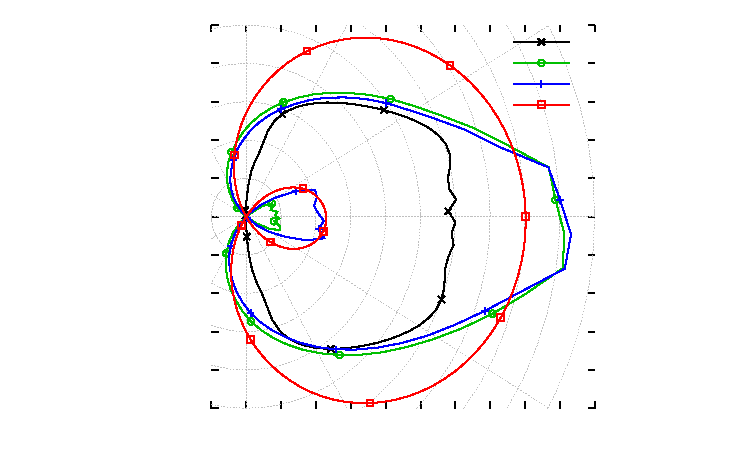
\includegraphics{/Users/seth/_thesis/figures/crashpipe2b/intens-x1-t1/intensity-x1-t1.pdf}}%
    \gplfronttext
  \end{picture}%
\endgroup
}%
  \subfloat[$t=15$]{%
    \hspace{-.25in}%
    % GNUPLOT: LaTeX picture with Postscript
\begingroup
  \makeatletter
  \providecommand\color[2][]{%
    \GenericError{(gnuplot) \space\space\space\@spaces}{%
      Package color not loaded in conjunction with
      terminal option `colourtext'%
    }{See the gnuplot documentation for explanation.%
    }{Either use 'blacktext' in gnuplot or load the package
      color.sty in LaTeX.}%
    \renewcommand\color[2][]{}%
  }%
  \providecommand\includegraphics[2][]{%
    \GenericError{(gnuplot) \space\space\space\@spaces}{%
      Package graphicx or graphics not loaded%
    }{See the gnuplot documentation for explanation.%
    }{The gnuplot epslatex terminal needs graphicx.sty or graphics.sty.}%
    \renewcommand\includegraphics[2][]{}%
  }%
  \providecommand\rotatebox[2]{#2}%
  \@ifundefined{ifGPcolor}{%
    \newif\ifGPcolor
    \GPcolortrue
  }{}%
  \@ifundefined{ifGPblacktext}{%
    \newif\ifGPblacktext
    \GPblacktexttrue
  }{}%
  % define a \g@addto@macro without @ in the name:
  \let\gplgaddtomacro\g@addto@macro
  % define empty templates for all commands taking text:
  \gdef\gplbacktext{}%
  \gdef\gplfronttext{}%
  \makeatother
  \ifGPblacktext
    % no textcolor at all
    \def\colorrgb#1{}%
    \def\colorgray#1{}%
  \else
    % gray or color?
    \ifGPcolor
      \def\colorrgb#1{\color[rgb]{#1}}%
      \def\colorgray#1{\color[gray]{#1}}%
      \expandafter\def\csname LTw\endcsname{\color{white}}%
      \expandafter\def\csname LTb\endcsname{\color{black}}%
      \expandafter\def\csname LTa\endcsname{\color{black}}%
      \expandafter\def\csname LT0\endcsname{\color[rgb]{1,0,0}}%
      \expandafter\def\csname LT1\endcsname{\color[rgb]{0,1,0}}%
      \expandafter\def\csname LT2\endcsname{\color[rgb]{0,0,1}}%
      \expandafter\def\csname LT3\endcsname{\color[rgb]{1,0,1}}%
      \expandafter\def\csname LT4\endcsname{\color[rgb]{0,1,1}}%
      \expandafter\def\csname LT5\endcsname{\color[rgb]{1,1,0}}%
      \expandafter\def\csname LT6\endcsname{\color[rgb]{0,0,0}}%
      \expandafter\def\csname LT7\endcsname{\color[rgb]{1,0.3,0}}%
      \expandafter\def\csname LT8\endcsname{\color[rgb]{0.5,0.5,0.5}}%
    \else
      % gray
      \def\colorrgb#1{\color{black}}%
      \def\colorgray#1{\color[gray]{#1}}%
      \expandafter\def\csname LTw\endcsname{\color{white}}%
      \expandafter\def\csname LTb\endcsname{\color{black}}%
      \expandafter\def\csname LTa\endcsname{\color{black}}%
      \expandafter\def\csname LT0\endcsname{\color{black}}%
      \expandafter\def\csname LT1\endcsname{\color{black}}%
      \expandafter\def\csname LT2\endcsname{\color{black}}%
      \expandafter\def\csname LT3\endcsname{\color{black}}%
      \expandafter\def\csname LT4\endcsname{\color{black}}%
      \expandafter\def\csname LT5\endcsname{\color{black}}%
      \expandafter\def\csname LT6\endcsname{\color{black}}%
      \expandafter\def\csname LT7\endcsname{\color{black}}%
      \expandafter\def\csname LT8\endcsname{\color{black}}%
    \fi
  \fi
  \setlength{\unitlength}{0.0500bp}%
  \begin{picture}(7200.00,4320.00)%
    \gplgaddtomacro\gplbacktext{%
      \csname LTb\endcsname%
      \put(1910,400){\makebox(0,0)[r]{\strut{} 0.1}}%
      \put(1910,768){\makebox(0,0)[r]{\strut{} 0.08}}%
      \put(1910,1136){\makebox(0,0)[r]{\strut{} 0.06}}%
      \put(1910,1504){\makebox(0,0)[r]{\strut{} 0.04}}%
      \put(1910,1872){\makebox(0,0)[r]{\strut{} 0.02}}%
      \put(1910,2240){\makebox(0,0)[r]{\strut{} 0}}%
      \put(1910,2607){\makebox(0,0)[r]{\strut{} 0.02}}%
      \put(1910,2975){\makebox(0,0)[r]{\strut{} 0.04}}%
      \put(1910,3343){\makebox(0,0)[r]{\strut{} 0.06}}%
      \put(1910,3711){\makebox(0,0)[r]{\strut{} 0.08}}%
      \put(1910,4079){\makebox(0,0)[r]{\strut{} 0.1}}%
      \csname LTb\endcsname%
      \put(2030,200){\makebox(0,0){\strut{} 0.02}}%
      \csname LTb\endcsname%
      \put(2364,200){\makebox(0,0){\strut{} 0}}%
      \csname LTb\endcsname%
      \put(2699,200){\makebox(0,0){\strut{} 0.02}}%
      \csname LTb\endcsname%
      \put(3033,200){\makebox(0,0){\strut{} 0.04}}%
      \csname LTb\endcsname%
      \put(3368,200){\makebox(0,0){\strut{} 0.06}}%
      \csname LTb\endcsname%
      \put(3702,200){\makebox(0,0){\strut{} 0.08}}%
      \csname LTb\endcsname%
      \put(4037,200){\makebox(0,0){\strut{} 0.1}}%
      \csname LTb\endcsname%
      \put(4371,200){\makebox(0,0){\strut{} 0.12}}%
      \csname LTb\endcsname%
      \put(4706,200){\makebox(0,0){\strut{} 0.14}}%
      \csname LTb\endcsname%
      \put(5040,200){\makebox(0,0){\strut{} 0.16}}%
      \csname LTb\endcsname%
      \put(5375,200){\makebox(0,0){\strut{} 0.18}}%
      \csname LTb\endcsname%
      \put(5709,200){\makebox(0,0){\strut{} 0.2}}%
      \csname LTb\endcsname%
      \put(1330,2239){\rotatebox{-270}{\makebox(0,0){\strut{}x1 center $(1.01,3.5)$}}}%
    }%
    \gplgaddtomacro\gplfronttext{%
      \csname LTb\endcsname%
      \put(4806,3916){\makebox(0,0)[r]{\strut{}S$_{128}$}}%
      \csname LTb\endcsname%
      \put(4806,3716){\makebox(0,0)[r]{\strut{}FLAD$_{64}$}}%
      \csname LTb\endcsname%
      \put(4806,3516){\makebox(0,0)[r]{\strut{}AD$_{64}$}}%
      \csname LTb\endcsname%
      \put(4806,3316){\makebox(0,0)[r]{\strut{}FLD}}%
    }%
    \gplbacktext
    \put(0,0){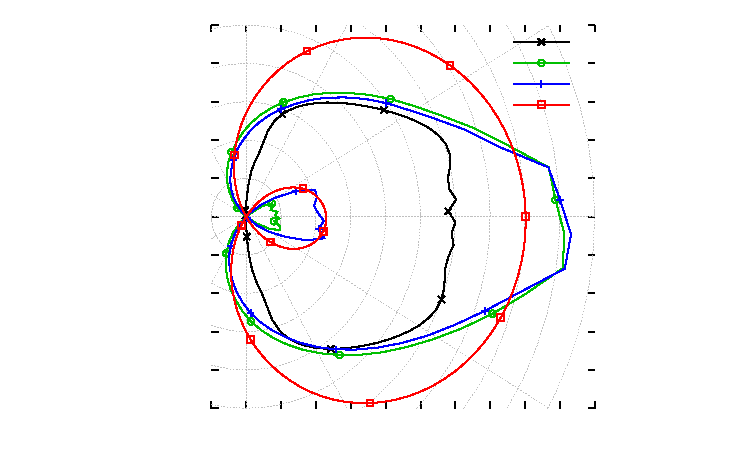
\includegraphics{/Users/seth/_thesis/figures/crashpipe2b/intens-x1-t1/intensity-x1-t1.pdf}}%
    \gplfronttext
  \end{picture}%
\endgroup
}

  \caption{Scalar intensity $\phi$ along the centerline of the channel, $y=2.5$.}
  \label{fig:tdReactor}
\end{figure}

None of the low-order methods exactly reproduces the transport solution. Even
with flux
limiting, FLD and FLAD overestimate the rate of particles flowing into the void.
However, as the problem tends toward steady-state, the anisotropic
methods become relatively accurate. (We recall that both FLAD and \APone\ limit
to the AD method when the solution varies slowly in time.)

A contour plot showing the difference between \Pone\ and \APone\ is given in
Fig.~\ref{fig:tdReactorContour}. The \APone\ solution is generally more accurate
than \Pone. As the system evolves in time, it becomes like the steady-state
channel problems analyzed earlier: diffusion (the steady-state limit of \Pone)
fails in these problems, so it is unsurprising that \APone\ outperforms \Pone\
at late times.

\begin{figure}[htb]
  \centering%\small

  \subfloat[$t=2$]{%
    \hspace{.75in}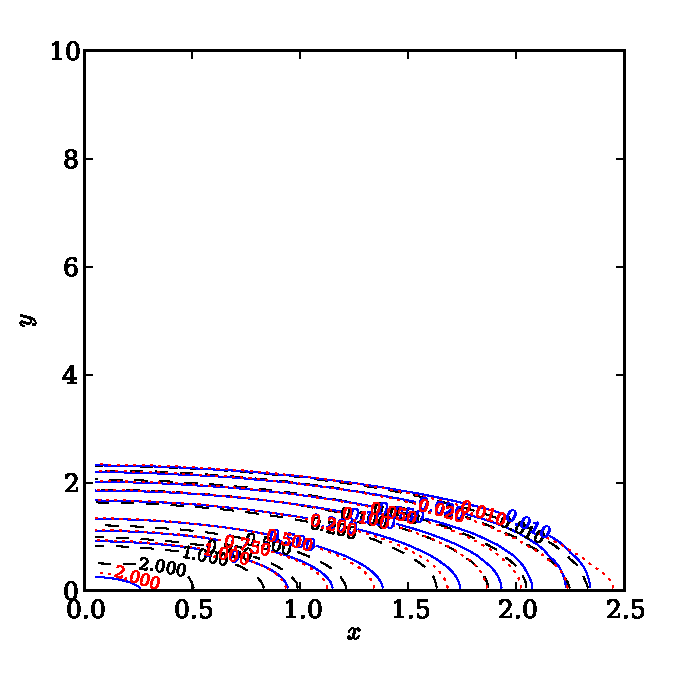
\includegraphics{td_reactor/phi-002}\hspace{.75in}}%
  \subfloat[$t=5$]{%
    \hspace{.75in}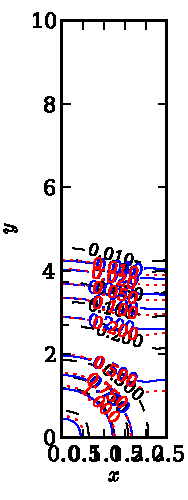
\includegraphics{td_reactor/phi-005}\hspace{.75in}}

  \subfloat[$t=10$]{%
    \hspace{.75in}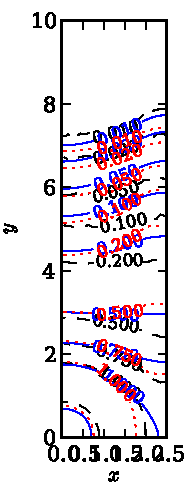
\includegraphics{td_reactor/phi-010}\hspace{.75in}}%
  \subfloat[$t=15$]{%
    \hspace{.75in}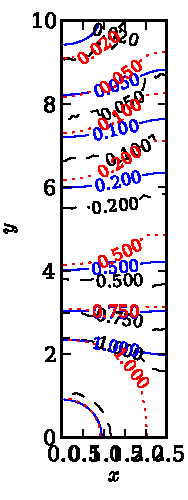
\includegraphics{td_reactor/phi-015}\hspace{.75in}}

  \Caption{Contour plots of the scalar intensity at four times.}{
    The black dashed line is the Monte Carlo solution, the blue solid line is
    the \APone\ solution, and the red dotted line is the \Pone\ solution.}
  \label{fig:tdReactorContour}
\end{figure}

As a final diagnostic, we plot the ``wavefront'' positions---determined by the
location at which $\phi=0.001$ after applying a small amount of smoothing---for
all of the methods in Fig.~\ref{fig:tdReactorWavefront}. These plots again show
how FLAD and AD both overestimate the scalar flux at early times, and they also
point to an explanation. Because the flux limiters are not iterated upon, the
solution of the first time step is the same as the standard diffusion
solution. (In Fig.~\ref{fig:tdReactorWavefrontLeft}, the flux-limited and
standard diffusion methods share a starting point.) As a result, the
flux-limited methods carry that artifact of non-flux-limited particles for all
later time steps. To obviate this error, shorter initial time steps (in which
the effective time absorption $1/c\Delta_t$ reduces the magnitude of the
precursor) could be used. Alternatively, the nonlinear flux-limited diffusion
coefficient could be converged.

\begin{figure}[htb]
  \centering\small
  \hspace{.25in}%
  \subfloat[Channel, $x=2.5$]{%
    \hspace{-.25in}%
    % GNUPLOT: LaTeX picture with Postscript
\begingroup
  \makeatletter
  \providecommand\color[2][]{%
    \GenericError{(gnuplot) \space\space\space\@spaces}{%
      Package color not loaded in conjunction with
      terminal option `colourtext'%
    }{See the gnuplot documentation for explanation.%
    }{Either use 'blacktext' in gnuplot or load the package
      color.sty in LaTeX.}%
    \renewcommand\color[2][]{}%
  }%
  \providecommand\includegraphics[2][]{%
    \GenericError{(gnuplot) \space\space\space\@spaces}{%
      Package graphicx or graphics not loaded%
    }{See the gnuplot documentation for explanation.%
    }{The gnuplot epslatex terminal needs graphicx.sty or graphics.sty.}%
    \renewcommand\includegraphics[2][]{}%
  }%
  \providecommand\rotatebox[2]{#2}%
  \@ifundefined{ifGPcolor}{%
    \newif\ifGPcolor
    \GPcolortrue
  }{}%
  \@ifundefined{ifGPblacktext}{%
    \newif\ifGPblacktext
    \GPblacktexttrue
  }{}%
  % define a \g@addto@macro without @ in the name:
  \let\gplgaddtomacro\g@addto@macro
  % define empty templates for all commands taking text:
  \gdef\gplbacktext{}%
  \gdef\gplfronttext{}%
  \makeatother
  \ifGPblacktext
    % no textcolor at all
    \def\colorrgb#1{}%
    \def\colorgray#1{}%
  \else
    % gray or color?
    \ifGPcolor
      \def\colorrgb#1{\color[rgb]{#1}}%
      \def\colorgray#1{\color[gray]{#1}}%
      \expandafter\def\csname LTw\endcsname{\color{white}}%
      \expandafter\def\csname LTb\endcsname{\color{black}}%
      \expandafter\def\csname LTa\endcsname{\color{black}}%
      \expandafter\def\csname LT0\endcsname{\color[rgb]{1,0,0}}%
      \expandafter\def\csname LT1\endcsname{\color[rgb]{0,1,0}}%
      \expandafter\def\csname LT2\endcsname{\color[rgb]{0,0,1}}%
      \expandafter\def\csname LT3\endcsname{\color[rgb]{1,0,1}}%
      \expandafter\def\csname LT4\endcsname{\color[rgb]{0,1,1}}%
      \expandafter\def\csname LT5\endcsname{\color[rgb]{1,1,0}}%
      \expandafter\def\csname LT6\endcsname{\color[rgb]{0,0,0}}%
      \expandafter\def\csname LT7\endcsname{\color[rgb]{1,0.3,0}}%
      \expandafter\def\csname LT8\endcsname{\color[rgb]{0.5,0.5,0.5}}%
    \else
      % gray
      \def\colorrgb#1{\color{black}}%
      \def\colorgray#1{\color[gray]{#1}}%
      \expandafter\def\csname LTw\endcsname{\color{white}}%
      \expandafter\def\csname LTb\endcsname{\color{black}}%
      \expandafter\def\csname LTa\endcsname{\color{black}}%
      \expandafter\def\csname LT0\endcsname{\color{black}}%
      \expandafter\def\csname LT1\endcsname{\color{black}}%
      \expandafter\def\csname LT2\endcsname{\color{black}}%
      \expandafter\def\csname LT3\endcsname{\color{black}}%
      \expandafter\def\csname LT4\endcsname{\color{black}}%
      \expandafter\def\csname LT5\endcsname{\color{black}}%
      \expandafter\def\csname LT6\endcsname{\color{black}}%
      \expandafter\def\csname LT7\endcsname{\color{black}}%
      \expandafter\def\csname LT8\endcsname{\color{black}}%
    \fi
  \fi
  \setlength{\unitlength}{0.0500bp}%
  \begin{picture}(7200.00,4320.00)%
    \gplgaddtomacro\gplbacktext{%
      \csname LTb\endcsname%
      \put(1910,400){\makebox(0,0)[r]{\strut{} 0.1}}%
      \put(1910,768){\makebox(0,0)[r]{\strut{} 0.08}}%
      \put(1910,1136){\makebox(0,0)[r]{\strut{} 0.06}}%
      \put(1910,1504){\makebox(0,0)[r]{\strut{} 0.04}}%
      \put(1910,1872){\makebox(0,0)[r]{\strut{} 0.02}}%
      \put(1910,2240){\makebox(0,0)[r]{\strut{} 0}}%
      \put(1910,2607){\makebox(0,0)[r]{\strut{} 0.02}}%
      \put(1910,2975){\makebox(0,0)[r]{\strut{} 0.04}}%
      \put(1910,3343){\makebox(0,0)[r]{\strut{} 0.06}}%
      \put(1910,3711){\makebox(0,0)[r]{\strut{} 0.08}}%
      \put(1910,4079){\makebox(0,0)[r]{\strut{} 0.1}}%
      \csname LTb\endcsname%
      \put(2030,200){\makebox(0,0){\strut{} 0.02}}%
      \csname LTb\endcsname%
      \put(2364,200){\makebox(0,0){\strut{} 0}}%
      \csname LTb\endcsname%
      \put(2699,200){\makebox(0,0){\strut{} 0.02}}%
      \csname LTb\endcsname%
      \put(3033,200){\makebox(0,0){\strut{} 0.04}}%
      \csname LTb\endcsname%
      \put(3368,200){\makebox(0,0){\strut{} 0.06}}%
      \csname LTb\endcsname%
      \put(3702,200){\makebox(0,0){\strut{} 0.08}}%
      \csname LTb\endcsname%
      \put(4037,200){\makebox(0,0){\strut{} 0.1}}%
      \csname LTb\endcsname%
      \put(4371,200){\makebox(0,0){\strut{} 0.12}}%
      \csname LTb\endcsname%
      \put(4706,200){\makebox(0,0){\strut{} 0.14}}%
      \csname LTb\endcsname%
      \put(5040,200){\makebox(0,0){\strut{} 0.16}}%
      \csname LTb\endcsname%
      \put(5375,200){\makebox(0,0){\strut{} 0.18}}%
      \csname LTb\endcsname%
      \put(5709,200){\makebox(0,0){\strut{} 0.2}}%
      \csname LTb\endcsname%
      \put(1330,2239){\rotatebox{-270}{\makebox(0,0){\strut{}x1 center $(1.01,3.5)$}}}%
    }%
    \gplgaddtomacro\gplfronttext{%
      \csname LTb\endcsname%
      \put(4806,3916){\makebox(0,0)[r]{\strut{}S$_{128}$}}%
      \csname LTb\endcsname%
      \put(4806,3716){\makebox(0,0)[r]{\strut{}FLAD$_{64}$}}%
      \csname LTb\endcsname%
      \put(4806,3516){\makebox(0,0)[r]{\strut{}AD$_{64}$}}%
      \csname LTb\endcsname%
      \put(4806,3316){\makebox(0,0)[r]{\strut{}FLD}}%
    }%
    \gplbacktext
    \put(0,0){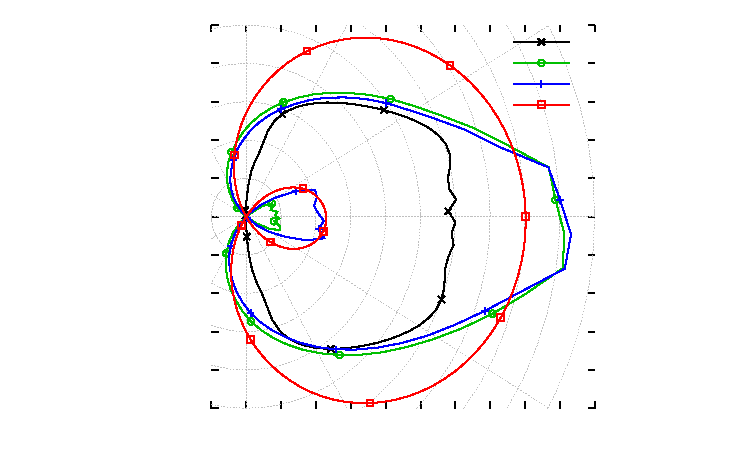
\includegraphics{/Users/seth/_thesis/figures/crashpipe2b/intens-x1-t1/intensity-x1-t1.pdf}}%
    \gplfronttext
  \end{picture}%
\endgroup
}
  \subfloat[Medium, $x=0$]{%
    \label{fig:tdReactorWavefrontLeft}%
    \hspace{-.25in}%
    % GNUPLOT: LaTeX picture with Postscript
\begingroup
  \makeatletter
  \providecommand\color[2][]{%
    \GenericError{(gnuplot) \space\space\space\@spaces}{%
      Package color not loaded in conjunction with
      terminal option `colourtext'%
    }{See the gnuplot documentation for explanation.%
    }{Either use 'blacktext' in gnuplot or load the package
      color.sty in LaTeX.}%
    \renewcommand\color[2][]{}%
  }%
  \providecommand\includegraphics[2][]{%
    \GenericError{(gnuplot) \space\space\space\@spaces}{%
      Package graphicx or graphics not loaded%
    }{See the gnuplot documentation for explanation.%
    }{The gnuplot epslatex terminal needs graphicx.sty or graphics.sty.}%
    \renewcommand\includegraphics[2][]{}%
  }%
  \providecommand\rotatebox[2]{#2}%
  \@ifundefined{ifGPcolor}{%
    \newif\ifGPcolor
    \GPcolortrue
  }{}%
  \@ifundefined{ifGPblacktext}{%
    \newif\ifGPblacktext
    \GPblacktexttrue
  }{}%
  % define a \g@addto@macro without @ in the name:
  \let\gplgaddtomacro\g@addto@macro
  % define empty templates for all commands taking text:
  \gdef\gplbacktext{}%
  \gdef\gplfronttext{}%
  \makeatother
  \ifGPblacktext
    % no textcolor at all
    \def\colorrgb#1{}%
    \def\colorgray#1{}%
  \else
    % gray or color?
    \ifGPcolor
      \def\colorrgb#1{\color[rgb]{#1}}%
      \def\colorgray#1{\color[gray]{#1}}%
      \expandafter\def\csname LTw\endcsname{\color{white}}%
      \expandafter\def\csname LTb\endcsname{\color{black}}%
      \expandafter\def\csname LTa\endcsname{\color{black}}%
      \expandafter\def\csname LT0\endcsname{\color[rgb]{1,0,0}}%
      \expandafter\def\csname LT1\endcsname{\color[rgb]{0,1,0}}%
      \expandafter\def\csname LT2\endcsname{\color[rgb]{0,0,1}}%
      \expandafter\def\csname LT3\endcsname{\color[rgb]{1,0,1}}%
      \expandafter\def\csname LT4\endcsname{\color[rgb]{0,1,1}}%
      \expandafter\def\csname LT5\endcsname{\color[rgb]{1,1,0}}%
      \expandafter\def\csname LT6\endcsname{\color[rgb]{0,0,0}}%
      \expandafter\def\csname LT7\endcsname{\color[rgb]{1,0.3,0}}%
      \expandafter\def\csname LT8\endcsname{\color[rgb]{0.5,0.5,0.5}}%
    \else
      % gray
      \def\colorrgb#1{\color{black}}%
      \def\colorgray#1{\color[gray]{#1}}%
      \expandafter\def\csname LTw\endcsname{\color{white}}%
      \expandafter\def\csname LTb\endcsname{\color{black}}%
      \expandafter\def\csname LTa\endcsname{\color{black}}%
      \expandafter\def\csname LT0\endcsname{\color{black}}%
      \expandafter\def\csname LT1\endcsname{\color{black}}%
      \expandafter\def\csname LT2\endcsname{\color{black}}%
      \expandafter\def\csname LT3\endcsname{\color{black}}%
      \expandafter\def\csname LT4\endcsname{\color{black}}%
      \expandafter\def\csname LT5\endcsname{\color{black}}%
      \expandafter\def\csname LT6\endcsname{\color{black}}%
      \expandafter\def\csname LT7\endcsname{\color{black}}%
      \expandafter\def\csname LT8\endcsname{\color{black}}%
    \fi
  \fi
  \setlength{\unitlength}{0.0500bp}%
  \begin{picture}(7200.00,4320.00)%
    \gplgaddtomacro\gplbacktext{%
      \csname LTb\endcsname%
      \put(1910,400){\makebox(0,0)[r]{\strut{} 0.1}}%
      \put(1910,768){\makebox(0,0)[r]{\strut{} 0.08}}%
      \put(1910,1136){\makebox(0,0)[r]{\strut{} 0.06}}%
      \put(1910,1504){\makebox(0,0)[r]{\strut{} 0.04}}%
      \put(1910,1872){\makebox(0,0)[r]{\strut{} 0.02}}%
      \put(1910,2240){\makebox(0,0)[r]{\strut{} 0}}%
      \put(1910,2607){\makebox(0,0)[r]{\strut{} 0.02}}%
      \put(1910,2975){\makebox(0,0)[r]{\strut{} 0.04}}%
      \put(1910,3343){\makebox(0,0)[r]{\strut{} 0.06}}%
      \put(1910,3711){\makebox(0,0)[r]{\strut{} 0.08}}%
      \put(1910,4079){\makebox(0,0)[r]{\strut{} 0.1}}%
      \csname LTb\endcsname%
      \put(2030,200){\makebox(0,0){\strut{} 0.02}}%
      \csname LTb\endcsname%
      \put(2364,200){\makebox(0,0){\strut{} 0}}%
      \csname LTb\endcsname%
      \put(2699,200){\makebox(0,0){\strut{} 0.02}}%
      \csname LTb\endcsname%
      \put(3033,200){\makebox(0,0){\strut{} 0.04}}%
      \csname LTb\endcsname%
      \put(3368,200){\makebox(0,0){\strut{} 0.06}}%
      \csname LTb\endcsname%
      \put(3702,200){\makebox(0,0){\strut{} 0.08}}%
      \csname LTb\endcsname%
      \put(4037,200){\makebox(0,0){\strut{} 0.1}}%
      \csname LTb\endcsname%
      \put(4371,200){\makebox(0,0){\strut{} 0.12}}%
      \csname LTb\endcsname%
      \put(4706,200){\makebox(0,0){\strut{} 0.14}}%
      \csname LTb\endcsname%
      \put(5040,200){\makebox(0,0){\strut{} 0.16}}%
      \csname LTb\endcsname%
      \put(5375,200){\makebox(0,0){\strut{} 0.18}}%
      \csname LTb\endcsname%
      \put(5709,200){\makebox(0,0){\strut{} 0.2}}%
      \csname LTb\endcsname%
      \put(1330,2239){\rotatebox{-270}{\makebox(0,0){\strut{}x1 center $(1.01,3.5)$}}}%
    }%
    \gplgaddtomacro\gplfronttext{%
      \csname LTb\endcsname%
      \put(4806,3916){\makebox(0,0)[r]{\strut{}S$_{128}$}}%
      \csname LTb\endcsname%
      \put(4806,3716){\makebox(0,0)[r]{\strut{}FLAD$_{64}$}}%
      \csname LTb\endcsname%
      \put(4806,3516){\makebox(0,0)[r]{\strut{}AD$_{64}$}}%
      \csname LTb\endcsname%
      \put(4806,3316){\makebox(0,0)[r]{\strut{}FLD}}%
    }%
    \gplbacktext
    \put(0,0){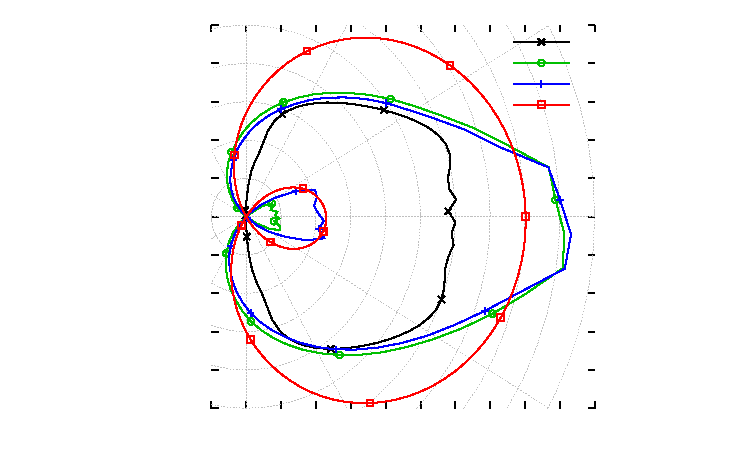
\includegraphics{/Users/seth/_thesis/figures/crashpipe2b/intens-x1-t1/intensity-x1-t1.pdf}}%
    \gplfronttext
  \end{picture}%
\endgroup
}
  \caption{Wavefront position along the $y$ axis.}
  \label{fig:tdReactorWavefront}
\end{figure}

%%%%%%%%%%%%%%%%%%%%%%%%%%%%%%%%%%%%%%%%%%%%%%%%%%%%%%%%%%%%%%%%%%%%%%%%%%%%%%%%
\clearpage
\section{Time-dependent blast wave}\label{sec:tdBlastwave}

Thermal radiative transfer problems often contain strong spatial and temporal
gradients. We consider a more stressful test of the different anisotropic
approximations to the transport equation.

\subsection{Problem description}

The ``blast wave'' test problem (Fig.~\ref{fig:tdBlastwaveXsn})
%
\begin{figure}[htb]
  \centering
  \includegraphics{td_blastpipe/xsn-enhanced}
  \Caption{Opacities and initial condition for the blast wave problem.}{
  The colored region is the isotropic initial condition $\phi_i$.}
  \label{fig:tdBlastwaveXsn}
\end{figure}
%
features a localized impulse of radiation; the
magnitude of the coefficients and the initial condition is based on a recurrent
test problem in the field
of thermal radiative transfer \cite{Kno1999a,Kno2001,Rau2005,Ols2007}. The
domain of this problem is $0 \le x \le 3$ and $-1.1 \le y \le 1.1$.
It features an optically thin channel with $\sigma=1$ and $\sigma_s=0.99$ inside
$-.1 \le y \le .1$, with a diffusive region $\sigma=10$ and $\sigma_s=9.99$
outside it. All boundaries are specularly reflecting.

The initial condition is a local but smooth Gaussian function:
\begin{equation*}
  \phi(x,y) = 0.001 + 100 \eexp^{-100 (x^2 + y^2) }\,.
\end{equation*}
We use a grid spacing of $\Delta_x=\Delta_y=0.02$, and a uniform time step
$\Delta_t=0.02$. As in the previous problem, the particle speed is $c=1$.

\subsection{Results and Discussion}

The isotropic initial condition is the only source of particles in this
problem. Because a majority of them are born in the optically thin channel,
those with directions close to the $+x$ axis will tend to stream down the
channel uncollided. This is the ``hyperbolic'' behavior of the transport
equation: when $\sigma$ and sources are small, it is a wave-like equation.
Particles that enter the medium diffuse: this is ``parabolic'' behavior. The
transport solution can be viewed as a combination of the hyperbolic and
parabolic solutions.

The final state ($t=3$) of the problem is plotted in Fig.~\ref{fig:tdBlastwave}.
Several features characteristic of the methods are apparent. First, only the
transport solution (Monte Carlo) contains the peak of uncollided particles at
$x=3$. Aside from that peak, the particles that have undergone
multiple collisions, the anisotropic diffusion methods all match reasonably
well. In this particular problem, flux-limited anisotropic diffusion is the most
accurate. The \Pone\ method fails even to produce a positive solution: this is a
known limitation of the method in multi-dimensional problems with strong spatial
and temporal gradients. Interestingly, the \APone\ solution is markedly better.
The smoothness of $\Dtens$ and $\varsigma$ as compared to $1/3\sigma$ and
$\sigma$ presumably obviate the strain on the wavelike behavior of the problem.

\begin{figure}[htb]
  \centering\small
  \subfloat[Along center]{%
    \hspace{-.25in}%
    % GNUPLOT: LaTeX picture with Postscript
\begingroup
  \makeatletter
  \providecommand\color[2][]{%
    \GenericError{(gnuplot) \space\space\space\@spaces}{%
      Package color not loaded in conjunction with
      terminal option `colourtext'%
    }{See the gnuplot documentation for explanation.%
    }{Either use 'blacktext' in gnuplot or load the package
      color.sty in LaTeX.}%
    \renewcommand\color[2][]{}%
  }%
  \providecommand\includegraphics[2][]{%
    \GenericError{(gnuplot) \space\space\space\@spaces}{%
      Package graphicx or graphics not loaded%
    }{See the gnuplot documentation for explanation.%
    }{The gnuplot epslatex terminal needs graphicx.sty or graphics.sty.}%
    \renewcommand\includegraphics[2][]{}%
  }%
  \providecommand\rotatebox[2]{#2}%
  \@ifundefined{ifGPcolor}{%
    \newif\ifGPcolor
    \GPcolortrue
  }{}%
  \@ifundefined{ifGPblacktext}{%
    \newif\ifGPblacktext
    \GPblacktexttrue
  }{}%
  % define a \g@addto@macro without @ in the name:
  \let\gplgaddtomacro\g@addto@macro
  % define empty templates for all commands taking text:
  \gdef\gplbacktext{}%
  \gdef\gplfronttext{}%
  \makeatother
  \ifGPblacktext
    % no textcolor at all
    \def\colorrgb#1{}%
    \def\colorgray#1{}%
  \else
    % gray or color?
    \ifGPcolor
      \def\colorrgb#1{\color[rgb]{#1}}%
      \def\colorgray#1{\color[gray]{#1}}%
      \expandafter\def\csname LTw\endcsname{\color{white}}%
      \expandafter\def\csname LTb\endcsname{\color{black}}%
      \expandafter\def\csname LTa\endcsname{\color{black}}%
      \expandafter\def\csname LT0\endcsname{\color[rgb]{1,0,0}}%
      \expandafter\def\csname LT1\endcsname{\color[rgb]{0,1,0}}%
      \expandafter\def\csname LT2\endcsname{\color[rgb]{0,0,1}}%
      \expandafter\def\csname LT3\endcsname{\color[rgb]{1,0,1}}%
      \expandafter\def\csname LT4\endcsname{\color[rgb]{0,1,1}}%
      \expandafter\def\csname LT5\endcsname{\color[rgb]{1,1,0}}%
      \expandafter\def\csname LT6\endcsname{\color[rgb]{0,0,0}}%
      \expandafter\def\csname LT7\endcsname{\color[rgb]{1,0.3,0}}%
      \expandafter\def\csname LT8\endcsname{\color[rgb]{0.5,0.5,0.5}}%
    \else
      % gray
      \def\colorrgb#1{\color{black}}%
      \def\colorgray#1{\color[gray]{#1}}%
      \expandafter\def\csname LTw\endcsname{\color{white}}%
      \expandafter\def\csname LTb\endcsname{\color{black}}%
      \expandafter\def\csname LTa\endcsname{\color{black}}%
      \expandafter\def\csname LT0\endcsname{\color{black}}%
      \expandafter\def\csname LT1\endcsname{\color{black}}%
      \expandafter\def\csname LT2\endcsname{\color{black}}%
      \expandafter\def\csname LT3\endcsname{\color{black}}%
      \expandafter\def\csname LT4\endcsname{\color{black}}%
      \expandafter\def\csname LT5\endcsname{\color{black}}%
      \expandafter\def\csname LT6\endcsname{\color{black}}%
      \expandafter\def\csname LT7\endcsname{\color{black}}%
      \expandafter\def\csname LT8\endcsname{\color{black}}%
    \fi
  \fi
  \setlength{\unitlength}{0.0500bp}%
  \begin{picture}(7200.00,4320.00)%
    \gplgaddtomacro\gplbacktext{%
      \csname LTb\endcsname%
      \put(1910,400){\makebox(0,0)[r]{\strut{} 0.1}}%
      \put(1910,768){\makebox(0,0)[r]{\strut{} 0.08}}%
      \put(1910,1136){\makebox(0,0)[r]{\strut{} 0.06}}%
      \put(1910,1504){\makebox(0,0)[r]{\strut{} 0.04}}%
      \put(1910,1872){\makebox(0,0)[r]{\strut{} 0.02}}%
      \put(1910,2240){\makebox(0,0)[r]{\strut{} 0}}%
      \put(1910,2607){\makebox(0,0)[r]{\strut{} 0.02}}%
      \put(1910,2975){\makebox(0,0)[r]{\strut{} 0.04}}%
      \put(1910,3343){\makebox(0,0)[r]{\strut{} 0.06}}%
      \put(1910,3711){\makebox(0,0)[r]{\strut{} 0.08}}%
      \put(1910,4079){\makebox(0,0)[r]{\strut{} 0.1}}%
      \csname LTb\endcsname%
      \put(2030,200){\makebox(0,0){\strut{} 0.02}}%
      \csname LTb\endcsname%
      \put(2364,200){\makebox(0,0){\strut{} 0}}%
      \csname LTb\endcsname%
      \put(2699,200){\makebox(0,0){\strut{} 0.02}}%
      \csname LTb\endcsname%
      \put(3033,200){\makebox(0,0){\strut{} 0.04}}%
      \csname LTb\endcsname%
      \put(3368,200){\makebox(0,0){\strut{} 0.06}}%
      \csname LTb\endcsname%
      \put(3702,200){\makebox(0,0){\strut{} 0.08}}%
      \csname LTb\endcsname%
      \put(4037,200){\makebox(0,0){\strut{} 0.1}}%
      \csname LTb\endcsname%
      \put(4371,200){\makebox(0,0){\strut{} 0.12}}%
      \csname LTb\endcsname%
      \put(4706,200){\makebox(0,0){\strut{} 0.14}}%
      \csname LTb\endcsname%
      \put(5040,200){\makebox(0,0){\strut{} 0.16}}%
      \csname LTb\endcsname%
      \put(5375,200){\makebox(0,0){\strut{} 0.18}}%
      \csname LTb\endcsname%
      \put(5709,200){\makebox(0,0){\strut{} 0.2}}%
      \csname LTb\endcsname%
      \put(1330,2239){\rotatebox{-270}{\makebox(0,0){\strut{}x1 center $(1.01,3.5)$}}}%
    }%
    \gplgaddtomacro\gplfronttext{%
      \csname LTb\endcsname%
      \put(4806,3916){\makebox(0,0)[r]{\strut{}S$_{128}$}}%
      \csname LTb\endcsname%
      \put(4806,3716){\makebox(0,0)[r]{\strut{}FLAD$_{64}$}}%
      \csname LTb\endcsname%
      \put(4806,3516){\makebox(0,0)[r]{\strut{}AD$_{64}$}}%
      \csname LTb\endcsname%
      \put(4806,3316){\makebox(0,0)[r]{\strut{}FLD}}%
    }%
    \gplbacktext
    \put(0,0){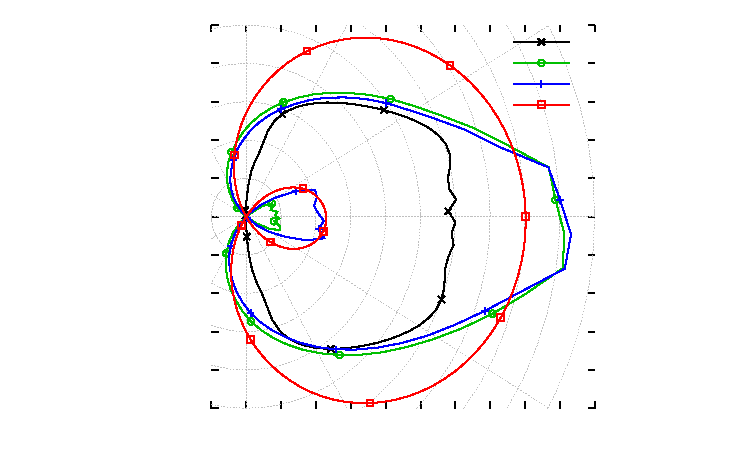
\includegraphics{/Users/seth/_thesis/figures/crashpipe2b/intens-x1-t1/intensity-x1-t1.pdf}}%
    \gplfronttext
  \end{picture}%
\endgroup
}%
  \subfloat[Orthogonal view]{%
    \hspace{-.25in}%
    % GNUPLOT: LaTeX picture with Postscript
\begingroup
  \makeatletter
  \providecommand\color[2][]{%
    \GenericError{(gnuplot) \space\space\space\@spaces}{%
      Package color not loaded in conjunction with
      terminal option `colourtext'%
    }{See the gnuplot documentation for explanation.%
    }{Either use 'blacktext' in gnuplot or load the package
      color.sty in LaTeX.}%
    \renewcommand\color[2][]{}%
  }%
  \providecommand\includegraphics[2][]{%
    \GenericError{(gnuplot) \space\space\space\@spaces}{%
      Package graphicx or graphics not loaded%
    }{See the gnuplot documentation for explanation.%
    }{The gnuplot epslatex terminal needs graphicx.sty or graphics.sty.}%
    \renewcommand\includegraphics[2][]{}%
  }%
  \providecommand\rotatebox[2]{#2}%
  \@ifundefined{ifGPcolor}{%
    \newif\ifGPcolor
    \GPcolortrue
  }{}%
  \@ifundefined{ifGPblacktext}{%
    \newif\ifGPblacktext
    \GPblacktexttrue
  }{}%
  % define a \g@addto@macro without @ in the name:
  \let\gplgaddtomacro\g@addto@macro
  % define empty templates for all commands taking text:
  \gdef\gplbacktext{}%
  \gdef\gplfronttext{}%
  \makeatother
  \ifGPblacktext
    % no textcolor at all
    \def\colorrgb#1{}%
    \def\colorgray#1{}%
  \else
    % gray or color?
    \ifGPcolor
      \def\colorrgb#1{\color[rgb]{#1}}%
      \def\colorgray#1{\color[gray]{#1}}%
      \expandafter\def\csname LTw\endcsname{\color{white}}%
      \expandafter\def\csname LTb\endcsname{\color{black}}%
      \expandafter\def\csname LTa\endcsname{\color{black}}%
      \expandafter\def\csname LT0\endcsname{\color[rgb]{1,0,0}}%
      \expandafter\def\csname LT1\endcsname{\color[rgb]{0,1,0}}%
      \expandafter\def\csname LT2\endcsname{\color[rgb]{0,0,1}}%
      \expandafter\def\csname LT3\endcsname{\color[rgb]{1,0,1}}%
      \expandafter\def\csname LT4\endcsname{\color[rgb]{0,1,1}}%
      \expandafter\def\csname LT5\endcsname{\color[rgb]{1,1,0}}%
      \expandafter\def\csname LT6\endcsname{\color[rgb]{0,0,0}}%
      \expandafter\def\csname LT7\endcsname{\color[rgb]{1,0.3,0}}%
      \expandafter\def\csname LT8\endcsname{\color[rgb]{0.5,0.5,0.5}}%
    \else
      % gray
      \def\colorrgb#1{\color{black}}%
      \def\colorgray#1{\color[gray]{#1}}%
      \expandafter\def\csname LTw\endcsname{\color{white}}%
      \expandafter\def\csname LTb\endcsname{\color{black}}%
      \expandafter\def\csname LTa\endcsname{\color{black}}%
      \expandafter\def\csname LT0\endcsname{\color{black}}%
      \expandafter\def\csname LT1\endcsname{\color{black}}%
      \expandafter\def\csname LT2\endcsname{\color{black}}%
      \expandafter\def\csname LT3\endcsname{\color{black}}%
      \expandafter\def\csname LT4\endcsname{\color{black}}%
      \expandafter\def\csname LT5\endcsname{\color{black}}%
      \expandafter\def\csname LT6\endcsname{\color{black}}%
      \expandafter\def\csname LT7\endcsname{\color{black}}%
      \expandafter\def\csname LT8\endcsname{\color{black}}%
    \fi
  \fi
  \setlength{\unitlength}{0.0500bp}%
  \begin{picture}(7200.00,4320.00)%
    \gplgaddtomacro\gplbacktext{%
      \csname LTb\endcsname%
      \put(1910,400){\makebox(0,0)[r]{\strut{} 0.1}}%
      \put(1910,768){\makebox(0,0)[r]{\strut{} 0.08}}%
      \put(1910,1136){\makebox(0,0)[r]{\strut{} 0.06}}%
      \put(1910,1504){\makebox(0,0)[r]{\strut{} 0.04}}%
      \put(1910,1872){\makebox(0,0)[r]{\strut{} 0.02}}%
      \put(1910,2240){\makebox(0,0)[r]{\strut{} 0}}%
      \put(1910,2607){\makebox(0,0)[r]{\strut{} 0.02}}%
      \put(1910,2975){\makebox(0,0)[r]{\strut{} 0.04}}%
      \put(1910,3343){\makebox(0,0)[r]{\strut{} 0.06}}%
      \put(1910,3711){\makebox(0,0)[r]{\strut{} 0.08}}%
      \put(1910,4079){\makebox(0,0)[r]{\strut{} 0.1}}%
      \csname LTb\endcsname%
      \put(2030,200){\makebox(0,0){\strut{} 0.02}}%
      \csname LTb\endcsname%
      \put(2364,200){\makebox(0,0){\strut{} 0}}%
      \csname LTb\endcsname%
      \put(2699,200){\makebox(0,0){\strut{} 0.02}}%
      \csname LTb\endcsname%
      \put(3033,200){\makebox(0,0){\strut{} 0.04}}%
      \csname LTb\endcsname%
      \put(3368,200){\makebox(0,0){\strut{} 0.06}}%
      \csname LTb\endcsname%
      \put(3702,200){\makebox(0,0){\strut{} 0.08}}%
      \csname LTb\endcsname%
      \put(4037,200){\makebox(0,0){\strut{} 0.1}}%
      \csname LTb\endcsname%
      \put(4371,200){\makebox(0,0){\strut{} 0.12}}%
      \csname LTb\endcsname%
      \put(4706,200){\makebox(0,0){\strut{} 0.14}}%
      \csname LTb\endcsname%
      \put(5040,200){\makebox(0,0){\strut{} 0.16}}%
      \csname LTb\endcsname%
      \put(5375,200){\makebox(0,0){\strut{} 0.18}}%
      \csname LTb\endcsname%
      \put(5709,200){\makebox(0,0){\strut{} 0.2}}%
      \csname LTb\endcsname%
      \put(1330,2239){\rotatebox{-270}{\makebox(0,0){\strut{}x1 center $(1.01,3.5)$}}}%
    }%
    \gplgaddtomacro\gplfronttext{%
      \csname LTb\endcsname%
      \put(4806,3916){\makebox(0,0)[r]{\strut{}S$_{128}$}}%
      \csname LTb\endcsname%
      \put(4806,3716){\makebox(0,0)[r]{\strut{}FLAD$_{64}$}}%
      \csname LTb\endcsname%
      \put(4806,3516){\makebox(0,0)[r]{\strut{}AD$_{64}$}}%
      \csname LTb\endcsname%
      \put(4806,3316){\makebox(0,0)[r]{\strut{}FLD}}%
    }%
    \gplbacktext
    \put(0,0){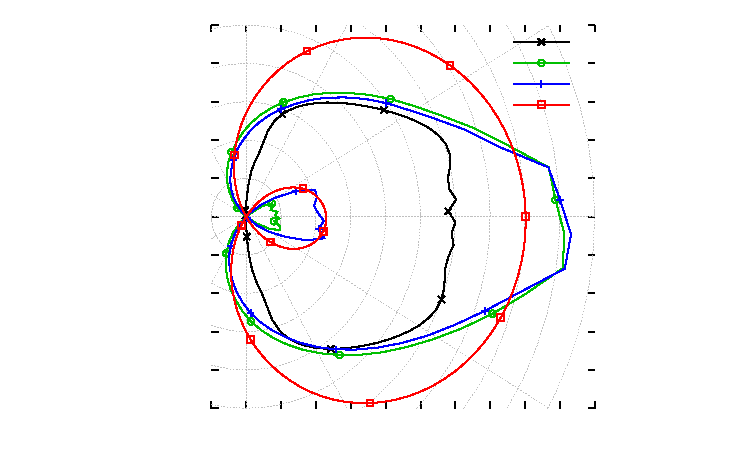
\includegraphics{/Users/seth/_thesis/figures/crashpipe2b/intens-x1-t1/intensity-x1-t1.pdf}}%
    \gplfronttext
  \end{picture}%
\endgroup
}%

  \caption{Scalar intensity at $t=3$ in the blast wave problem.}
  \label{fig:tdBlastwave}
\end{figure}

The time-dependent behavior of the transport solution (MC) and flux-limited
anisotropic diffusion (FLAD) is shown in Fig.~\ref{fig:tdBlastwaveAll}. At longer
times, the FLAD solution approaches the MC solution away from the uncollided
pulse of particles.

\begin{figure}[htb]
  \centering\small
    \hspace{-.15in}%
    % GNUPLOT: LaTeX picture with Postscript
\begingroup
  \makeatletter
  \providecommand\color[2][]{%
    \GenericError{(gnuplot) \space\space\space\@spaces}{%
      Package color not loaded in conjunction with
      terminal option `colourtext'%
    }{See the gnuplot documentation for explanation.%
    }{Either use 'blacktext' in gnuplot or load the package
      color.sty in LaTeX.}%
    \renewcommand\color[2][]{}%
  }%
  \providecommand\includegraphics[2][]{%
    \GenericError{(gnuplot) \space\space\space\@spaces}{%
      Package graphicx or graphics not loaded%
    }{See the gnuplot documentation for explanation.%
    }{The gnuplot epslatex terminal needs graphicx.sty or graphics.sty.}%
    \renewcommand\includegraphics[2][]{}%
  }%
  \providecommand\rotatebox[2]{#2}%
  \@ifundefined{ifGPcolor}{%
    \newif\ifGPcolor
    \GPcolortrue
  }{}%
  \@ifundefined{ifGPblacktext}{%
    \newif\ifGPblacktext
    \GPblacktexttrue
  }{}%
  % define a \g@addto@macro without @ in the name:
  \let\gplgaddtomacro\g@addto@macro
  % define empty templates for all commands taking text:
  \gdef\gplbacktext{}%
  \gdef\gplfronttext{}%
  \makeatother
  \ifGPblacktext
    % no textcolor at all
    \def\colorrgb#1{}%
    \def\colorgray#1{}%
  \else
    % gray or color?
    \ifGPcolor
      \def\colorrgb#1{\color[rgb]{#1}}%
      \def\colorgray#1{\color[gray]{#1}}%
      \expandafter\def\csname LTw\endcsname{\color{white}}%
      \expandafter\def\csname LTb\endcsname{\color{black}}%
      \expandafter\def\csname LTa\endcsname{\color{black}}%
      \expandafter\def\csname LT0\endcsname{\color[rgb]{1,0,0}}%
      \expandafter\def\csname LT1\endcsname{\color[rgb]{0,1,0}}%
      \expandafter\def\csname LT2\endcsname{\color[rgb]{0,0,1}}%
      \expandafter\def\csname LT3\endcsname{\color[rgb]{1,0,1}}%
      \expandafter\def\csname LT4\endcsname{\color[rgb]{0,1,1}}%
      \expandafter\def\csname LT5\endcsname{\color[rgb]{1,1,0}}%
      \expandafter\def\csname LT6\endcsname{\color[rgb]{0,0,0}}%
      \expandafter\def\csname LT7\endcsname{\color[rgb]{1,0.3,0}}%
      \expandafter\def\csname LT8\endcsname{\color[rgb]{0.5,0.5,0.5}}%
    \else
      % gray
      \def\colorrgb#1{\color{black}}%
      \def\colorgray#1{\color[gray]{#1}}%
      \expandafter\def\csname LTw\endcsname{\color{white}}%
      \expandafter\def\csname LTb\endcsname{\color{black}}%
      \expandafter\def\csname LTa\endcsname{\color{black}}%
      \expandafter\def\csname LT0\endcsname{\color{black}}%
      \expandafter\def\csname LT1\endcsname{\color{black}}%
      \expandafter\def\csname LT2\endcsname{\color{black}}%
      \expandafter\def\csname LT3\endcsname{\color{black}}%
      \expandafter\def\csname LT4\endcsname{\color{black}}%
      \expandafter\def\csname LT5\endcsname{\color{black}}%
      \expandafter\def\csname LT6\endcsname{\color{black}}%
      \expandafter\def\csname LT7\endcsname{\color{black}}%
      \expandafter\def\csname LT8\endcsname{\color{black}}%
    \fi
  \fi
  \setlength{\unitlength}{0.0500bp}%
  \begin{picture}(7200.00,4320.00)%
    \gplgaddtomacro\gplbacktext{%
      \csname LTb\endcsname%
      \put(1910,400){\makebox(0,0)[r]{\strut{} 0.1}}%
      \put(1910,768){\makebox(0,0)[r]{\strut{} 0.08}}%
      \put(1910,1136){\makebox(0,0)[r]{\strut{} 0.06}}%
      \put(1910,1504){\makebox(0,0)[r]{\strut{} 0.04}}%
      \put(1910,1872){\makebox(0,0)[r]{\strut{} 0.02}}%
      \put(1910,2240){\makebox(0,0)[r]{\strut{} 0}}%
      \put(1910,2607){\makebox(0,0)[r]{\strut{} 0.02}}%
      \put(1910,2975){\makebox(0,0)[r]{\strut{} 0.04}}%
      \put(1910,3343){\makebox(0,0)[r]{\strut{} 0.06}}%
      \put(1910,3711){\makebox(0,0)[r]{\strut{} 0.08}}%
      \put(1910,4079){\makebox(0,0)[r]{\strut{} 0.1}}%
      \csname LTb\endcsname%
      \put(2030,200){\makebox(0,0){\strut{} 0.02}}%
      \csname LTb\endcsname%
      \put(2364,200){\makebox(0,0){\strut{} 0}}%
      \csname LTb\endcsname%
      \put(2699,200){\makebox(0,0){\strut{} 0.02}}%
      \csname LTb\endcsname%
      \put(3033,200){\makebox(0,0){\strut{} 0.04}}%
      \csname LTb\endcsname%
      \put(3368,200){\makebox(0,0){\strut{} 0.06}}%
      \csname LTb\endcsname%
      \put(3702,200){\makebox(0,0){\strut{} 0.08}}%
      \csname LTb\endcsname%
      \put(4037,200){\makebox(0,0){\strut{} 0.1}}%
      \csname LTb\endcsname%
      \put(4371,200){\makebox(0,0){\strut{} 0.12}}%
      \csname LTb\endcsname%
      \put(4706,200){\makebox(0,0){\strut{} 0.14}}%
      \csname LTb\endcsname%
      \put(5040,200){\makebox(0,0){\strut{} 0.16}}%
      \csname LTb\endcsname%
      \put(5375,200){\makebox(0,0){\strut{} 0.18}}%
      \csname LTb\endcsname%
      \put(5709,200){\makebox(0,0){\strut{} 0.2}}%
      \csname LTb\endcsname%
      \put(1330,2239){\rotatebox{-270}{\makebox(0,0){\strut{}x1 center $(1.01,3.5)$}}}%
    }%
    \gplgaddtomacro\gplfronttext{%
      \csname LTb\endcsname%
      \put(4806,3916){\makebox(0,0)[r]{\strut{}S$_{128}$}}%
      \csname LTb\endcsname%
      \put(4806,3716){\makebox(0,0)[r]{\strut{}FLAD$_{64}$}}%
      \csname LTb\endcsname%
      \put(4806,3516){\makebox(0,0)[r]{\strut{}AD$_{64}$}}%
      \csname LTb\endcsname%
      \put(4806,3316){\makebox(0,0)[r]{\strut{}FLD}}%
    }%
    \gplbacktext
    \put(0,0){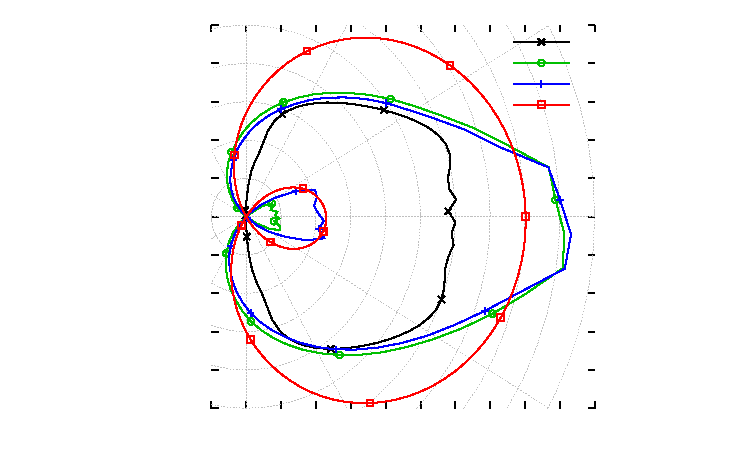
\includegraphics{/Users/seth/_thesis/figures/crashpipe2b/intens-x1-t1/intensity-x1-t1.pdf}}%
    \gplfronttext
  \end{picture}%
\endgroup


  \caption{Comparison of Monte Carlo and flux-limited anisotropic diffusion at
  four times in the blast wave problem.}
  \label{fig:tdBlastwaveAll}
\end{figure}

Because the diffusion equations are inherently parabolic, they cannot capture
the behavior of the uncollided particles seen in the Monte Carlo solution.
However, the hyperbolic (diffusive) behavior is modeled more accurately with
the AD methods than with conventional diffusion methods. As we have seen in the
previous test problems, the linear-in-angle approximation of standard diffusion
is wholly inadequate in the interior of the channel, leading to an inaccurate
solution.

The timings for the blast wave problem, as run on a single core of a 2.4 GHz
Intel Core 2 Duo chip, are presented in Table~\ref{tab:tdBlastwaveTiming}. These
give a rough idea of the relative performance of the standard diffusion methods,
the anisotropic diffusion methods, and the transport method. The initial
calculation of the anisotropic diffusion coefficients is amortized over the
subsequent time steps, so over longer times, the performance of the AD methods
asymptotically approaches the performance of the standard diffusion methods.

\begin{table}[htb]
  \centering
  \begin{tabular}{lr}
\toprule
    & Wall time (s)
\\ \midrule
MC & 790 \\
\APone & 31 \\
FLAD & 40 \\
AD & 38 \\
\Pone & 23 \\
FLD & 18 \\
Diffusion & 18
\\ \bottomrule
  \end{tabular}
  \caption{Timing comparison for the blast wave problem.}
  \label{tab:tdBlastwaveTiming}
\end{table}

\subsection{Extended problem parameter space}
To quantitatively verify that the positive results in this problem are not
accidental, we parameterized the problem and extensively investigated the parameter
space.
Using Latin Hypercube Sampling \cite{McK1979}, we sampled 40 instances of
the above problem with the following parameters and corresponding distributions:
\begin{itemize}
  \item the width of the diffusive region (uniform on $[0,2]$);
  \item the width of the channel region (uniform on $[0,1]$);
  \item the sharpness of the Gaussian (exponential with $\lambda = 100$);
  \item the value of $\sigma$ in the diffusive region (uniform on $[1,20]$); and
  \item the value of $\sigma$ in the channel region (exponential with
    $\lambda=0.1$).
\end{itemize}

As a metric of error, we compared the volume-weighted
2-norm error (with the reference solution being a Monte Carlo simulation
with $10^6$ particles) along the channel centerline and a cross-section of the
problem at $x=0.3$ at the final problem time. (Other metrics yielded similar
results.)

The error distributions are plotted in Fig.~\ref{fig:tdBlastwaveParameterized}.
%
\begin{figure}[htb]
  \centering\small
  \subfloat[Along center]{%
    \hspace{-.25in}%
    % GNUPLOT: LaTeX picture with Postscript
\begingroup
  \makeatletter
  \providecommand\color[2][]{%
    \GenericError{(gnuplot) \space\space\space\@spaces}{%
      Package color not loaded in conjunction with
      terminal option `colourtext'%
    }{See the gnuplot documentation for explanation.%
    }{Either use 'blacktext' in gnuplot or load the package
      color.sty in LaTeX.}%
    \renewcommand\color[2][]{}%
  }%
  \providecommand\includegraphics[2][]{%
    \GenericError{(gnuplot) \space\space\space\@spaces}{%
      Package graphicx or graphics not loaded%
    }{See the gnuplot documentation for explanation.%
    }{The gnuplot epslatex terminal needs graphicx.sty or graphics.sty.}%
    \renewcommand\includegraphics[2][]{}%
  }%
  \providecommand\rotatebox[2]{#2}%
  \@ifundefined{ifGPcolor}{%
    \newif\ifGPcolor
    \GPcolortrue
  }{}%
  \@ifundefined{ifGPblacktext}{%
    \newif\ifGPblacktext
    \GPblacktexttrue
  }{}%
  % define a \g@addto@macro without @ in the name:
  \let\gplgaddtomacro\g@addto@macro
  % define empty templates for all commands taking text:
  \gdef\gplbacktext{}%
  \gdef\gplfronttext{}%
  \makeatother
  \ifGPblacktext
    % no textcolor at all
    \def\colorrgb#1{}%
    \def\colorgray#1{}%
  \else
    % gray or color?
    \ifGPcolor
      \def\colorrgb#1{\color[rgb]{#1}}%
      \def\colorgray#1{\color[gray]{#1}}%
      \expandafter\def\csname LTw\endcsname{\color{white}}%
      \expandafter\def\csname LTb\endcsname{\color{black}}%
      \expandafter\def\csname LTa\endcsname{\color{black}}%
      \expandafter\def\csname LT0\endcsname{\color[rgb]{1,0,0}}%
      \expandafter\def\csname LT1\endcsname{\color[rgb]{0,1,0}}%
      \expandafter\def\csname LT2\endcsname{\color[rgb]{0,0,1}}%
      \expandafter\def\csname LT3\endcsname{\color[rgb]{1,0,1}}%
      \expandafter\def\csname LT4\endcsname{\color[rgb]{0,1,1}}%
      \expandafter\def\csname LT5\endcsname{\color[rgb]{1,1,0}}%
      \expandafter\def\csname LT6\endcsname{\color[rgb]{0,0,0}}%
      \expandafter\def\csname LT7\endcsname{\color[rgb]{1,0.3,0}}%
      \expandafter\def\csname LT8\endcsname{\color[rgb]{0.5,0.5,0.5}}%
    \else
      % gray
      \def\colorrgb#1{\color{black}}%
      \def\colorgray#1{\color[gray]{#1}}%
      \expandafter\def\csname LTw\endcsname{\color{white}}%
      \expandafter\def\csname LTb\endcsname{\color{black}}%
      \expandafter\def\csname LTa\endcsname{\color{black}}%
      \expandafter\def\csname LT0\endcsname{\color{black}}%
      \expandafter\def\csname LT1\endcsname{\color{black}}%
      \expandafter\def\csname LT2\endcsname{\color{black}}%
      \expandafter\def\csname LT3\endcsname{\color{black}}%
      \expandafter\def\csname LT4\endcsname{\color{black}}%
      \expandafter\def\csname LT5\endcsname{\color{black}}%
      \expandafter\def\csname LT6\endcsname{\color{black}}%
      \expandafter\def\csname LT7\endcsname{\color{black}}%
      \expandafter\def\csname LT8\endcsname{\color{black}}%
    \fi
  \fi
  \setlength{\unitlength}{0.0500bp}%
  \begin{picture}(7200.00,4320.00)%
    \gplgaddtomacro\gplbacktext{%
      \csname LTb\endcsname%
      \put(1910,400){\makebox(0,0)[r]{\strut{} 0.1}}%
      \put(1910,768){\makebox(0,0)[r]{\strut{} 0.08}}%
      \put(1910,1136){\makebox(0,0)[r]{\strut{} 0.06}}%
      \put(1910,1504){\makebox(0,0)[r]{\strut{} 0.04}}%
      \put(1910,1872){\makebox(0,0)[r]{\strut{} 0.02}}%
      \put(1910,2240){\makebox(0,0)[r]{\strut{} 0}}%
      \put(1910,2607){\makebox(0,0)[r]{\strut{} 0.02}}%
      \put(1910,2975){\makebox(0,0)[r]{\strut{} 0.04}}%
      \put(1910,3343){\makebox(0,0)[r]{\strut{} 0.06}}%
      \put(1910,3711){\makebox(0,0)[r]{\strut{} 0.08}}%
      \put(1910,4079){\makebox(0,0)[r]{\strut{} 0.1}}%
      \csname LTb\endcsname%
      \put(2030,200){\makebox(0,0){\strut{} 0.02}}%
      \csname LTb\endcsname%
      \put(2364,200){\makebox(0,0){\strut{} 0}}%
      \csname LTb\endcsname%
      \put(2699,200){\makebox(0,0){\strut{} 0.02}}%
      \csname LTb\endcsname%
      \put(3033,200){\makebox(0,0){\strut{} 0.04}}%
      \csname LTb\endcsname%
      \put(3368,200){\makebox(0,0){\strut{} 0.06}}%
      \csname LTb\endcsname%
      \put(3702,200){\makebox(0,0){\strut{} 0.08}}%
      \csname LTb\endcsname%
      \put(4037,200){\makebox(0,0){\strut{} 0.1}}%
      \csname LTb\endcsname%
      \put(4371,200){\makebox(0,0){\strut{} 0.12}}%
      \csname LTb\endcsname%
      \put(4706,200){\makebox(0,0){\strut{} 0.14}}%
      \csname LTb\endcsname%
      \put(5040,200){\makebox(0,0){\strut{} 0.16}}%
      \csname LTb\endcsname%
      \put(5375,200){\makebox(0,0){\strut{} 0.18}}%
      \csname LTb\endcsname%
      \put(5709,200){\makebox(0,0){\strut{} 0.2}}%
      \csname LTb\endcsname%
      \put(1330,2239){\rotatebox{-270}{\makebox(0,0){\strut{}x1 center $(1.01,3.5)$}}}%
    }%
    \gplgaddtomacro\gplfronttext{%
      \csname LTb\endcsname%
      \put(4806,3916){\makebox(0,0)[r]{\strut{}S$_{128}$}}%
      \csname LTb\endcsname%
      \put(4806,3716){\makebox(0,0)[r]{\strut{}FLAD$_{64}$}}%
      \csname LTb\endcsname%
      \put(4806,3516){\makebox(0,0)[r]{\strut{}AD$_{64}$}}%
      \csname LTb\endcsname%
      \put(4806,3316){\makebox(0,0)[r]{\strut{}FLD}}%
    }%
    \gplbacktext
    \put(0,0){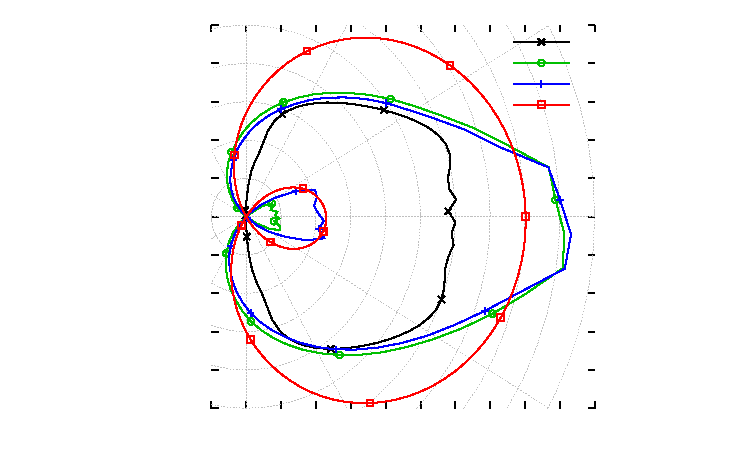
\includegraphics{/Users/seth/_thesis/figures/crashpipe2b/intens-x1-t1/intensity-x1-t1.pdf}}%
    \gplfronttext
  \end{picture}%
\endgroup
}%
  \subfloat[Orthogonal view]{%
    \hspace{-.25in}%
    % GNUPLOT: LaTeX picture with Postscript
\begingroup
  \makeatletter
  \providecommand\color[2][]{%
    \GenericError{(gnuplot) \space\space\space\@spaces}{%
      Package color not loaded in conjunction with
      terminal option `colourtext'%
    }{See the gnuplot documentation for explanation.%
    }{Either use 'blacktext' in gnuplot or load the package
      color.sty in LaTeX.}%
    \renewcommand\color[2][]{}%
  }%
  \providecommand\includegraphics[2][]{%
    \GenericError{(gnuplot) \space\space\space\@spaces}{%
      Package graphicx or graphics not loaded%
    }{See the gnuplot documentation for explanation.%
    }{The gnuplot epslatex terminal needs graphicx.sty or graphics.sty.}%
    \renewcommand\includegraphics[2][]{}%
  }%
  \providecommand\rotatebox[2]{#2}%
  \@ifundefined{ifGPcolor}{%
    \newif\ifGPcolor
    \GPcolortrue
  }{}%
  \@ifundefined{ifGPblacktext}{%
    \newif\ifGPblacktext
    \GPblacktexttrue
  }{}%
  % define a \g@addto@macro without @ in the name:
  \let\gplgaddtomacro\g@addto@macro
  % define empty templates for all commands taking text:
  \gdef\gplbacktext{}%
  \gdef\gplfronttext{}%
  \makeatother
  \ifGPblacktext
    % no textcolor at all
    \def\colorrgb#1{}%
    \def\colorgray#1{}%
  \else
    % gray or color?
    \ifGPcolor
      \def\colorrgb#1{\color[rgb]{#1}}%
      \def\colorgray#1{\color[gray]{#1}}%
      \expandafter\def\csname LTw\endcsname{\color{white}}%
      \expandafter\def\csname LTb\endcsname{\color{black}}%
      \expandafter\def\csname LTa\endcsname{\color{black}}%
      \expandafter\def\csname LT0\endcsname{\color[rgb]{1,0,0}}%
      \expandafter\def\csname LT1\endcsname{\color[rgb]{0,1,0}}%
      \expandafter\def\csname LT2\endcsname{\color[rgb]{0,0,1}}%
      \expandafter\def\csname LT3\endcsname{\color[rgb]{1,0,1}}%
      \expandafter\def\csname LT4\endcsname{\color[rgb]{0,1,1}}%
      \expandafter\def\csname LT5\endcsname{\color[rgb]{1,1,0}}%
      \expandafter\def\csname LT6\endcsname{\color[rgb]{0,0,0}}%
      \expandafter\def\csname LT7\endcsname{\color[rgb]{1,0.3,0}}%
      \expandafter\def\csname LT8\endcsname{\color[rgb]{0.5,0.5,0.5}}%
    \else
      % gray
      \def\colorrgb#1{\color{black}}%
      \def\colorgray#1{\color[gray]{#1}}%
      \expandafter\def\csname LTw\endcsname{\color{white}}%
      \expandafter\def\csname LTb\endcsname{\color{black}}%
      \expandafter\def\csname LTa\endcsname{\color{black}}%
      \expandafter\def\csname LT0\endcsname{\color{black}}%
      \expandafter\def\csname LT1\endcsname{\color{black}}%
      \expandafter\def\csname LT2\endcsname{\color{black}}%
      \expandafter\def\csname LT3\endcsname{\color{black}}%
      \expandafter\def\csname LT4\endcsname{\color{black}}%
      \expandafter\def\csname LT5\endcsname{\color{black}}%
      \expandafter\def\csname LT6\endcsname{\color{black}}%
      \expandafter\def\csname LT7\endcsname{\color{black}}%
      \expandafter\def\csname LT8\endcsname{\color{black}}%
    \fi
  \fi
  \setlength{\unitlength}{0.0500bp}%
  \begin{picture}(7200.00,4320.00)%
    \gplgaddtomacro\gplbacktext{%
      \csname LTb\endcsname%
      \put(1910,400){\makebox(0,0)[r]{\strut{} 0.1}}%
      \put(1910,768){\makebox(0,0)[r]{\strut{} 0.08}}%
      \put(1910,1136){\makebox(0,0)[r]{\strut{} 0.06}}%
      \put(1910,1504){\makebox(0,0)[r]{\strut{} 0.04}}%
      \put(1910,1872){\makebox(0,0)[r]{\strut{} 0.02}}%
      \put(1910,2240){\makebox(0,0)[r]{\strut{} 0}}%
      \put(1910,2607){\makebox(0,0)[r]{\strut{} 0.02}}%
      \put(1910,2975){\makebox(0,0)[r]{\strut{} 0.04}}%
      \put(1910,3343){\makebox(0,0)[r]{\strut{} 0.06}}%
      \put(1910,3711){\makebox(0,0)[r]{\strut{} 0.08}}%
      \put(1910,4079){\makebox(0,0)[r]{\strut{} 0.1}}%
      \csname LTb\endcsname%
      \put(2030,200){\makebox(0,0){\strut{} 0.02}}%
      \csname LTb\endcsname%
      \put(2364,200){\makebox(0,0){\strut{} 0}}%
      \csname LTb\endcsname%
      \put(2699,200){\makebox(0,0){\strut{} 0.02}}%
      \csname LTb\endcsname%
      \put(3033,200){\makebox(0,0){\strut{} 0.04}}%
      \csname LTb\endcsname%
      \put(3368,200){\makebox(0,0){\strut{} 0.06}}%
      \csname LTb\endcsname%
      \put(3702,200){\makebox(0,0){\strut{} 0.08}}%
      \csname LTb\endcsname%
      \put(4037,200){\makebox(0,0){\strut{} 0.1}}%
      \csname LTb\endcsname%
      \put(4371,200){\makebox(0,0){\strut{} 0.12}}%
      \csname LTb\endcsname%
      \put(4706,200){\makebox(0,0){\strut{} 0.14}}%
      \csname LTb\endcsname%
      \put(5040,200){\makebox(0,0){\strut{} 0.16}}%
      \csname LTb\endcsname%
      \put(5375,200){\makebox(0,0){\strut{} 0.18}}%
      \csname LTb\endcsname%
      \put(5709,200){\makebox(0,0){\strut{} 0.2}}%
      \csname LTb\endcsname%
      \put(1330,2239){\rotatebox{-270}{\makebox(0,0){\strut{}x1 center $(1.01,3.5)$}}}%
    }%
    \gplgaddtomacro\gplfronttext{%
      \csname LTb\endcsname%
      \put(4806,3916){\makebox(0,0)[r]{\strut{}S$_{128}$}}%
      \csname LTb\endcsname%
      \put(4806,3716){\makebox(0,0)[r]{\strut{}FLAD$_{64}$}}%
      \csname LTb\endcsname%
      \put(4806,3516){\makebox(0,0)[r]{\strut{}AD$_{64}$}}%
      \csname LTb\endcsname%
      \put(4806,3316){\makebox(0,0)[r]{\strut{}FLD}}%
    }%
    \gplbacktext
    \put(0,0){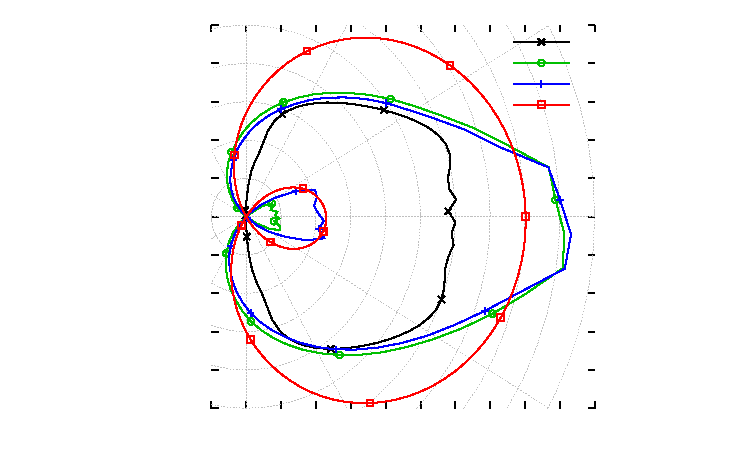
\includegraphics{/Users/seth/_thesis/figures/crashpipe2b/intens-x1-t1/intensity-x1-t1.pdf}}%
    \gplfronttext
  \end{picture}%
\endgroup
}%

  \caption{Distributions of errors in the parameterized blast wave problem.}
  \label{fig:tdBlastwaveParameterized}
\end{figure}
%
Distributions more peaked toward the left of the plot are more accurate, and
wider distributions indicate a method inconsistent in its accuracy. As one might
expect from the detailed discussion of one instance of the blast wave problem,
flux-limited anisotropic diffusion is the most accurate, and \Pone\ is the least
accurate.

%%%%%%%%%%%%%%%%%%%%%%%%%%%%%%%%%%%%%%%%%%%%%%%%%%%%%%%%%%%%%%%%%%%%%%%%%%%%%%%%
\section{Conclusions}

We have established and tested some approximations that undergird the rest of
our results.  First, we ensured that non-analytic (discrete
ordinates--calculated) AD coefficients do not compromise the accuracy of the
method. We also demonstrated that the number of sweeps required to converge a
transport-calculated $f$ is small enough to make an AD solution competitive.

With the linear numerical experiments in this chapter, we have verified the
theory developed in the previous chapters. The boundary conditions we proposed
for anisotropic diffusion in Chapter~\ref{chap:adDerivation} yield accurate
answers for our test problems in which the radiation is not strongly anisotropic
throughout the problem. The boundary conditions for flatland diffusion were also
successfully tested.

Finally, we performed the first test of time-dependent anisotropic diffusion. In
a wide variety of problems with optically thin channels, the anisotropic
diffusion methods (particularly flux-limited anisotropic diffusion) outperformed
their conventional counterparts.

With these encouraging results for linear, time-dependent problems, we move to
more difficult non-linear problems in Chapter~\ref{chap:trtNumericalResults}.


% !TEX root = _individual/trtNumericalResults.tex
% !TEX root = thesis.tex
%\addtocounter{page}{-1}
%%%%%%%%%%%%%%%%%%%%%%%%%%%%%%%%%%%%%%%%%%%%%%%%%%%%%%%%%%%%%%%%%%%%%%%%%%%%%%%%
\chapter{Numerical results: thermal radiative transfer}
\label{chap:trtNumericalResults}

Thermal radiative transfer, as we discussed at length in
Chapter~\ref{chap:trtBackground}, adds complexities beyond the already
substantial
difficulties of particle transport. The radiation source term is coupled to a
material temperature unknown, and the material's changing temperature modifies
the absorption opacity. These nonlinearities require special treatment
(semi-implicit linearization, in our work), and they mean that the problem's
physical properties are time-dependent. For the anisotropic diffusion methods,
this imposes the extra requirement that the diffusion coefficients be
recalculated at every time step.

In this chapter we test a wide range of TRT problems, beginning with diffusive
1-D problems that
contain temperature-dependent opacities. In addition to testing multi-D problems
with optically thin channels, we compare the performance of the anisotropic
methods against conventional methods using standard 2-D TRT benchmark problems.
%We also assess the performance of the methods in a realistic problem of
%interest.

Most of the methods we compare are described at the start of
Chapter~\ref{chap:simpleNumericalResults}, but the following methods need
further discussion when applied to TRT.
\begin{description}

  \item[Monte Carlo] is replaced by Implicit Monte Carlo \cite{Fle1971}. Our
    implementation uses implicit absorption, source tilting, census combing, and
    energy-weighted path length tallies \cite{Urb2006}. Each problem uses
    roughly $10^7$ particles per time step.

  \item[Anisotropic methods] Because the opacity is a time-dependent quantity
in TRT, the anisotropic diffusion coefficients must be recalculated at every
time step. The first time step uses up to 100 source iteration sweeps%
\footnote{%
  This is a \emph{very} conservative number; as the previous chapter showed,
  two or three iterations are sufficient.
} to
calculate the coefficients, but each time step thereafter uses only one sweep to
update them. (Because the transport problem for $f$ is purely absorbing, one
sweep is sufficient to converge the diffusion coefficients in the interior.)

  \item[\Pone-like methods] A known shortcoming of \Pone\ is that, in
    multidimensional geometry with steep gradients, the radiation can have a
    negative solution \cite{McC2008a}. To prevent unphysical negative
    temperatures, we
    ``fix'' non-positive values for the radiation by setting them
    to $10^{-16}$, violating conservation by adding energy to the problem.

\end{description}

%%%%%%%%%%%%%%%%%%%%%%%%%%%%%%%%%%%%%%%%%%%%%%%%%%%%%%%%%%%%%%%%%%%%%%%%%%%%%%%%
\section{1-D blast wave}\label{sec:trtOned}
We begin by testing a simple one-dimensional slab geometry problem on a refined
spatial and temporal grid. The anisotropic diffusion approximation is less
meaningful in 1-D: the rank-2 tensor becomes a scalar. Nevertheless, the AD
coefficient is still nonlocal and distinct from the standard diffusion
coefficient.

The classic Marshak wave \cite{Mar1958} is a feature of radiative transfer at
the boundaries between hot and cold materials. Because the cold material tends
to be optically opaque, radiation emitted from the hot material penetrates only
a short distance into the cold, rapidly heating it. As that layer of cold
material heats up, it begins to emit into the adjacent cold layer: the result
is a distinct radiation shock that looks like a wave. (Because the radiation
behavior tends to be diffusive rather than streaming, this wave does not
travel at the speed of light.)

This 1-D test problem does not create a ``classic'' Marshak wave: rather than a
constant
incident radiation boundary, it contains a large pulse of energy as an initial
condition. Yet the resulting qualitative behavior strongly resembles a Marshak
wave, since the pulse penetrates the colder material and heats it up
progressively.

Higher-dimensional geometries also have Marshak wave--like behavior, so the
features observed in this one-dimensional problem serves as a useful
introduction to the behavior of the different methods tested.

%%%%%%%%%%%%%%%%%%%%%%%%%%%%%%%%%%%%%%%%
\subsection{Problem description}
This ``diffusive'' test problem has been used to assess the
performance of flux limiters and nonlinear convergence schemes
\cite{Rau2005,Ols2007}. It features a smooth but
localized energy peak as an initial condition in both the material and the
radiation:
\begin{equation*}
  \phi(x,0) = [ a c T(x,0)]^{4} = 0.001 + 100 \eexp^{-100 x^2} \,.
\end{equation*}
The material is uniform with a constant heat capacity $c_v = 1$ and a
temperature-dependent
opacity $\sigma(T) = T^{-3}$. We use a uniform spatial and temporal grid of
$\Delta_x = \Delta_t = 0.01$. The boundaries at $x=0$ and $x=3$ are reflecting.

The problem uses a scaled unit system often seen in TRT methods development: $c
= a = 1$. The anisotropic diffusion coefficients are calculated with a
Gauss--Legendre $S_{16}$ quadrature set and the step characteristics method.

%%%%%%%%%%%%%%%%%%%%%%%%%%%%%%%%%%%%%%%%
\subsection{Results and discussion}

The wavefront position (Fig.~\ref{fig:1dblastWavefront}) provides an effective
%
\begin{figure}[tb]
  \centering\small
  % GNUPLOT: LaTeX picture with Postscript
\begingroup
  \makeatletter
  \providecommand\color[2][]{%
    \GenericError{(gnuplot) \space\space\space\@spaces}{%
      Package color not loaded in conjunction with
      terminal option `colourtext'%
    }{See the gnuplot documentation for explanation.%
    }{Either use 'blacktext' in gnuplot or load the package
      color.sty in LaTeX.}%
    \renewcommand\color[2][]{}%
  }%
  \providecommand\includegraphics[2][]{%
    \GenericError{(gnuplot) \space\space\space\@spaces}{%
      Package graphicx or graphics not loaded%
    }{See the gnuplot documentation for explanation.%
    }{The gnuplot epslatex terminal needs graphicx.sty or graphics.sty.}%
    \renewcommand\includegraphics[2][]{}%
  }%
  \providecommand\rotatebox[2]{#2}%
  \@ifundefined{ifGPcolor}{%
    \newif\ifGPcolor
    \GPcolortrue
  }{}%
  \@ifundefined{ifGPblacktext}{%
    \newif\ifGPblacktext
    \GPblacktexttrue
  }{}%
  % define a \g@addto@macro without @ in the name:
  \let\gplgaddtomacro\g@addto@macro
  % define empty templates for all commands taking text:
  \gdef\gplbacktext{}%
  \gdef\gplfronttext{}%
  \makeatother
  \ifGPblacktext
    % no textcolor at all
    \def\colorrgb#1{}%
    \def\colorgray#1{}%
  \else
    % gray or color?
    \ifGPcolor
      \def\colorrgb#1{\color[rgb]{#1}}%
      \def\colorgray#1{\color[gray]{#1}}%
      \expandafter\def\csname LTw\endcsname{\color{white}}%
      \expandafter\def\csname LTb\endcsname{\color{black}}%
      \expandafter\def\csname LTa\endcsname{\color{black}}%
      \expandafter\def\csname LT0\endcsname{\color[rgb]{1,0,0}}%
      \expandafter\def\csname LT1\endcsname{\color[rgb]{0,1,0}}%
      \expandafter\def\csname LT2\endcsname{\color[rgb]{0,0,1}}%
      \expandafter\def\csname LT3\endcsname{\color[rgb]{1,0,1}}%
      \expandafter\def\csname LT4\endcsname{\color[rgb]{0,1,1}}%
      \expandafter\def\csname LT5\endcsname{\color[rgb]{1,1,0}}%
      \expandafter\def\csname LT6\endcsname{\color[rgb]{0,0,0}}%
      \expandafter\def\csname LT7\endcsname{\color[rgb]{1,0.3,0}}%
      \expandafter\def\csname LT8\endcsname{\color[rgb]{0.5,0.5,0.5}}%
    \else
      % gray
      \def\colorrgb#1{\color{black}}%
      \def\colorgray#1{\color[gray]{#1}}%
      \expandafter\def\csname LTw\endcsname{\color{white}}%
      \expandafter\def\csname LTb\endcsname{\color{black}}%
      \expandafter\def\csname LTa\endcsname{\color{black}}%
      \expandafter\def\csname LT0\endcsname{\color{black}}%
      \expandafter\def\csname LT1\endcsname{\color{black}}%
      \expandafter\def\csname LT2\endcsname{\color{black}}%
      \expandafter\def\csname LT3\endcsname{\color{black}}%
      \expandafter\def\csname LT4\endcsname{\color{black}}%
      \expandafter\def\csname LT5\endcsname{\color{black}}%
      \expandafter\def\csname LT6\endcsname{\color{black}}%
      \expandafter\def\csname LT7\endcsname{\color{black}}%
      \expandafter\def\csname LT8\endcsname{\color{black}}%
    \fi
  \fi
  \setlength{\unitlength}{0.0500bp}%
  \begin{picture}(7200.00,4320.00)%
    \gplgaddtomacro\gplbacktext{%
      \csname LTb\endcsname%
      \put(1910,400){\makebox(0,0)[r]{\strut{} 0.1}}%
      \put(1910,768){\makebox(0,0)[r]{\strut{} 0.08}}%
      \put(1910,1136){\makebox(0,0)[r]{\strut{} 0.06}}%
      \put(1910,1504){\makebox(0,0)[r]{\strut{} 0.04}}%
      \put(1910,1872){\makebox(0,0)[r]{\strut{} 0.02}}%
      \put(1910,2240){\makebox(0,0)[r]{\strut{} 0}}%
      \put(1910,2607){\makebox(0,0)[r]{\strut{} 0.02}}%
      \put(1910,2975){\makebox(0,0)[r]{\strut{} 0.04}}%
      \put(1910,3343){\makebox(0,0)[r]{\strut{} 0.06}}%
      \put(1910,3711){\makebox(0,0)[r]{\strut{} 0.08}}%
      \put(1910,4079){\makebox(0,0)[r]{\strut{} 0.1}}%
      \csname LTb\endcsname%
      \put(2030,200){\makebox(0,0){\strut{} 0.02}}%
      \csname LTb\endcsname%
      \put(2364,200){\makebox(0,0){\strut{} 0}}%
      \csname LTb\endcsname%
      \put(2699,200){\makebox(0,0){\strut{} 0.02}}%
      \csname LTb\endcsname%
      \put(3033,200){\makebox(0,0){\strut{} 0.04}}%
      \csname LTb\endcsname%
      \put(3368,200){\makebox(0,0){\strut{} 0.06}}%
      \csname LTb\endcsname%
      \put(3702,200){\makebox(0,0){\strut{} 0.08}}%
      \csname LTb\endcsname%
      \put(4037,200){\makebox(0,0){\strut{} 0.1}}%
      \csname LTb\endcsname%
      \put(4371,200){\makebox(0,0){\strut{} 0.12}}%
      \csname LTb\endcsname%
      \put(4706,200){\makebox(0,0){\strut{} 0.14}}%
      \csname LTb\endcsname%
      \put(5040,200){\makebox(0,0){\strut{} 0.16}}%
      \csname LTb\endcsname%
      \put(5375,200){\makebox(0,0){\strut{} 0.18}}%
      \csname LTb\endcsname%
      \put(5709,200){\makebox(0,0){\strut{} 0.2}}%
      \csname LTb\endcsname%
      \put(1330,2239){\rotatebox{-270}{\makebox(0,0){\strut{}x1 center $(1.01,3.5)$}}}%
    }%
    \gplgaddtomacro\gplfronttext{%
      \csname LTb\endcsname%
      \put(4806,3916){\makebox(0,0)[r]{\strut{}S$_{128}$}}%
      \csname LTb\endcsname%
      \put(4806,3716){\makebox(0,0)[r]{\strut{}FLAD$_{64}$}}%
      \csname LTb\endcsname%
      \put(4806,3516){\makebox(0,0)[r]{\strut{}AD$_{64}$}}%
      \csname LTb\endcsname%
      \put(4806,3316){\makebox(0,0)[r]{\strut{}FLD}}%
    }%
    \gplbacktext
    \put(0,0){\includegraphics{/Users/seth/_thesis/figures/crashpipe2b/intens-x1-t1/intensity-x1-t1.pdf}}%
    \gplfronttext
  \end{picture}%
\endgroup

  \caption{Wavefront position of $\phi$ in 1-D blast wave problem.}
  \label{fig:1dblastWavefront}
\end{figure}
%
visualization of the problem's time evolution. The position is calculated at
each point in time by taking the radiation temperature, convolving it with a
weighted five-point kernel to smooth out potential noise in the solution, and
using linear interpolation to find the point at which the radiation temperature
is twice the initial temperature of the problem.

We note how Fig.~\ref{fig:1dblastWavefront}
shows that, during the streaming-dominated early times, both standard diffusion
and anisotropic diffusion display an unphysical wave speed. For these methods,
the slope of the wavefront position near $t=0$ exceeds $c=1$: energy is
transferred through the system faster than the speed of light. This
shortcoming motivated the development of both flux-limited diffusion
(\S\ref{sec:bgFld}) and our flux-limited anisotropic diffusion
(\S\ref{sec:flad}). Both the standard \Pone\ and anisotropic \Pone\ are wave
equations, but they have the incorrect wave speed of $c/\sqrt{3}$.

A detailed view of the radiation and material temperatures
(Fig.~\ref{fig:1dblastTemp}) at $t=3$ gives further insight into the differences
%
\begin{figure}[tb]
  \centering\small
  \centering
  \subfloat[Radiation temperature]{%
    \hspace{-.25in}%
    % GNUPLOT: LaTeX picture with Postscript
\begingroup
  \makeatletter
  \providecommand\color[2][]{%
    \GenericError{(gnuplot) \space\space\space\@spaces}{%
      Package color not loaded in conjunction with
      terminal option `colourtext'%
    }{See the gnuplot documentation for explanation.%
    }{Either use 'blacktext' in gnuplot or load the package
      color.sty in LaTeX.}%
    \renewcommand\color[2][]{}%
  }%
  \providecommand\includegraphics[2][]{%
    \GenericError{(gnuplot) \space\space\space\@spaces}{%
      Package graphicx or graphics not loaded%
    }{See the gnuplot documentation for explanation.%
    }{The gnuplot epslatex terminal needs graphicx.sty or graphics.sty.}%
    \renewcommand\includegraphics[2][]{}%
  }%
  \providecommand\rotatebox[2]{#2}%
  \@ifundefined{ifGPcolor}{%
    \newif\ifGPcolor
    \GPcolortrue
  }{}%
  \@ifundefined{ifGPblacktext}{%
    \newif\ifGPblacktext
    \GPblacktexttrue
  }{}%
  % define a \g@addto@macro without @ in the name:
  \let\gplgaddtomacro\g@addto@macro
  % define empty templates for all commands taking text:
  \gdef\gplbacktext{}%
  \gdef\gplfronttext{}%
  \makeatother
  \ifGPblacktext
    % no textcolor at all
    \def\colorrgb#1{}%
    \def\colorgray#1{}%
  \else
    % gray or color?
    \ifGPcolor
      \def\colorrgb#1{\color[rgb]{#1}}%
      \def\colorgray#1{\color[gray]{#1}}%
      \expandafter\def\csname LTw\endcsname{\color{white}}%
      \expandafter\def\csname LTb\endcsname{\color{black}}%
      \expandafter\def\csname LTa\endcsname{\color{black}}%
      \expandafter\def\csname LT0\endcsname{\color[rgb]{1,0,0}}%
      \expandafter\def\csname LT1\endcsname{\color[rgb]{0,1,0}}%
      \expandafter\def\csname LT2\endcsname{\color[rgb]{0,0,1}}%
      \expandafter\def\csname LT3\endcsname{\color[rgb]{1,0,1}}%
      \expandafter\def\csname LT4\endcsname{\color[rgb]{0,1,1}}%
      \expandafter\def\csname LT5\endcsname{\color[rgb]{1,1,0}}%
      \expandafter\def\csname LT6\endcsname{\color[rgb]{0,0,0}}%
      \expandafter\def\csname LT7\endcsname{\color[rgb]{1,0.3,0}}%
      \expandafter\def\csname LT8\endcsname{\color[rgb]{0.5,0.5,0.5}}%
    \else
      % gray
      \def\colorrgb#1{\color{black}}%
      \def\colorgray#1{\color[gray]{#1}}%
      \expandafter\def\csname LTw\endcsname{\color{white}}%
      \expandafter\def\csname LTb\endcsname{\color{black}}%
      \expandafter\def\csname LTa\endcsname{\color{black}}%
      \expandafter\def\csname LT0\endcsname{\color{black}}%
      \expandafter\def\csname LT1\endcsname{\color{black}}%
      \expandafter\def\csname LT2\endcsname{\color{black}}%
      \expandafter\def\csname LT3\endcsname{\color{black}}%
      \expandafter\def\csname LT4\endcsname{\color{black}}%
      \expandafter\def\csname LT5\endcsname{\color{black}}%
      \expandafter\def\csname LT6\endcsname{\color{black}}%
      \expandafter\def\csname LT7\endcsname{\color{black}}%
      \expandafter\def\csname LT8\endcsname{\color{black}}%
    \fi
  \fi
  \setlength{\unitlength}{0.0500bp}%
  \begin{picture}(7200.00,4320.00)%
    \gplgaddtomacro\gplbacktext{%
      \csname LTb\endcsname%
      \put(1910,400){\makebox(0,0)[r]{\strut{} 0.1}}%
      \put(1910,768){\makebox(0,0)[r]{\strut{} 0.08}}%
      \put(1910,1136){\makebox(0,0)[r]{\strut{} 0.06}}%
      \put(1910,1504){\makebox(0,0)[r]{\strut{} 0.04}}%
      \put(1910,1872){\makebox(0,0)[r]{\strut{} 0.02}}%
      \put(1910,2240){\makebox(0,0)[r]{\strut{} 0}}%
      \put(1910,2607){\makebox(0,0)[r]{\strut{} 0.02}}%
      \put(1910,2975){\makebox(0,0)[r]{\strut{} 0.04}}%
      \put(1910,3343){\makebox(0,0)[r]{\strut{} 0.06}}%
      \put(1910,3711){\makebox(0,0)[r]{\strut{} 0.08}}%
      \put(1910,4079){\makebox(0,0)[r]{\strut{} 0.1}}%
      \csname LTb\endcsname%
      \put(2030,200){\makebox(0,0){\strut{} 0.02}}%
      \csname LTb\endcsname%
      \put(2364,200){\makebox(0,0){\strut{} 0}}%
      \csname LTb\endcsname%
      \put(2699,200){\makebox(0,0){\strut{} 0.02}}%
      \csname LTb\endcsname%
      \put(3033,200){\makebox(0,0){\strut{} 0.04}}%
      \csname LTb\endcsname%
      \put(3368,200){\makebox(0,0){\strut{} 0.06}}%
      \csname LTb\endcsname%
      \put(3702,200){\makebox(0,0){\strut{} 0.08}}%
      \csname LTb\endcsname%
      \put(4037,200){\makebox(0,0){\strut{} 0.1}}%
      \csname LTb\endcsname%
      \put(4371,200){\makebox(0,0){\strut{} 0.12}}%
      \csname LTb\endcsname%
      \put(4706,200){\makebox(0,0){\strut{} 0.14}}%
      \csname LTb\endcsname%
      \put(5040,200){\makebox(0,0){\strut{} 0.16}}%
      \csname LTb\endcsname%
      \put(5375,200){\makebox(0,0){\strut{} 0.18}}%
      \csname LTb\endcsname%
      \put(5709,200){\makebox(0,0){\strut{} 0.2}}%
      \csname LTb\endcsname%
      \put(1330,2239){\rotatebox{-270}{\makebox(0,0){\strut{}x1 center $(1.01,3.5)$}}}%
    }%
    \gplgaddtomacro\gplfronttext{%
      \csname LTb\endcsname%
      \put(4806,3916){\makebox(0,0)[r]{\strut{}S$_{128}$}}%
      \csname LTb\endcsname%
      \put(4806,3716){\makebox(0,0)[r]{\strut{}FLAD$_{64}$}}%
      \csname LTb\endcsname%
      \put(4806,3516){\makebox(0,0)[r]{\strut{}AD$_{64}$}}%
      \csname LTb\endcsname%
      \put(4806,3316){\makebox(0,0)[r]{\strut{}FLD}}%
    }%
    \gplbacktext
    \put(0,0){\includegraphics{/Users/seth/_thesis/figures/crashpipe2b/intens-x1-t1/intensity-x1-t1.pdf}}%
    \gplfronttext
  \end{picture}%
\endgroup

  }%
  \subfloat[Material temperature]{%
    \hspace{-.25in}%
    % GNUPLOT: LaTeX picture with Postscript
\begingroup
  \makeatletter
  \providecommand\color[2][]{%
    \GenericError{(gnuplot) \space\space\space\@spaces}{%
      Package color not loaded in conjunction with
      terminal option `colourtext'%
    }{See the gnuplot documentation for explanation.%
    }{Either use 'blacktext' in gnuplot or load the package
      color.sty in LaTeX.}%
    \renewcommand\color[2][]{}%
  }%
  \providecommand\includegraphics[2][]{%
    \GenericError{(gnuplot) \space\space\space\@spaces}{%
      Package graphicx or graphics not loaded%
    }{See the gnuplot documentation for explanation.%
    }{The gnuplot epslatex terminal needs graphicx.sty or graphics.sty.}%
    \renewcommand\includegraphics[2][]{}%
  }%
  \providecommand\rotatebox[2]{#2}%
  \@ifundefined{ifGPcolor}{%
    \newif\ifGPcolor
    \GPcolortrue
  }{}%
  \@ifundefined{ifGPblacktext}{%
    \newif\ifGPblacktext
    \GPblacktexttrue
  }{}%
  % define a \g@addto@macro without @ in the name:
  \let\gplgaddtomacro\g@addto@macro
  % define empty templates for all commands taking text:
  \gdef\gplbacktext{}%
  \gdef\gplfronttext{}%
  \makeatother
  \ifGPblacktext
    % no textcolor at all
    \def\colorrgb#1{}%
    \def\colorgray#1{}%
  \else
    % gray or color?
    \ifGPcolor
      \def\colorrgb#1{\color[rgb]{#1}}%
      \def\colorgray#1{\color[gray]{#1}}%
      \expandafter\def\csname LTw\endcsname{\color{white}}%
      \expandafter\def\csname LTb\endcsname{\color{black}}%
      \expandafter\def\csname LTa\endcsname{\color{black}}%
      \expandafter\def\csname LT0\endcsname{\color[rgb]{1,0,0}}%
      \expandafter\def\csname LT1\endcsname{\color[rgb]{0,1,0}}%
      \expandafter\def\csname LT2\endcsname{\color[rgb]{0,0,1}}%
      \expandafter\def\csname LT3\endcsname{\color[rgb]{1,0,1}}%
      \expandafter\def\csname LT4\endcsname{\color[rgb]{0,1,1}}%
      \expandafter\def\csname LT5\endcsname{\color[rgb]{1,1,0}}%
      \expandafter\def\csname LT6\endcsname{\color[rgb]{0,0,0}}%
      \expandafter\def\csname LT7\endcsname{\color[rgb]{1,0.3,0}}%
      \expandafter\def\csname LT8\endcsname{\color[rgb]{0.5,0.5,0.5}}%
    \else
      % gray
      \def\colorrgb#1{\color{black}}%
      \def\colorgray#1{\color[gray]{#1}}%
      \expandafter\def\csname LTw\endcsname{\color{white}}%
      \expandafter\def\csname LTb\endcsname{\color{black}}%
      \expandafter\def\csname LTa\endcsname{\color{black}}%
      \expandafter\def\csname LT0\endcsname{\color{black}}%
      \expandafter\def\csname LT1\endcsname{\color{black}}%
      \expandafter\def\csname LT2\endcsname{\color{black}}%
      \expandafter\def\csname LT3\endcsname{\color{black}}%
      \expandafter\def\csname LT4\endcsname{\color{black}}%
      \expandafter\def\csname LT5\endcsname{\color{black}}%
      \expandafter\def\csname LT6\endcsname{\color{black}}%
      \expandafter\def\csname LT7\endcsname{\color{black}}%
      \expandafter\def\csname LT8\endcsname{\color{black}}%
    \fi
  \fi
  \setlength{\unitlength}{0.0500bp}%
  \begin{picture}(7200.00,4320.00)%
    \gplgaddtomacro\gplbacktext{%
      \csname LTb\endcsname%
      \put(1910,400){\makebox(0,0)[r]{\strut{} 0.1}}%
      \put(1910,768){\makebox(0,0)[r]{\strut{} 0.08}}%
      \put(1910,1136){\makebox(0,0)[r]{\strut{} 0.06}}%
      \put(1910,1504){\makebox(0,0)[r]{\strut{} 0.04}}%
      \put(1910,1872){\makebox(0,0)[r]{\strut{} 0.02}}%
      \put(1910,2240){\makebox(0,0)[r]{\strut{} 0}}%
      \put(1910,2607){\makebox(0,0)[r]{\strut{} 0.02}}%
      \put(1910,2975){\makebox(0,0)[r]{\strut{} 0.04}}%
      \put(1910,3343){\makebox(0,0)[r]{\strut{} 0.06}}%
      \put(1910,3711){\makebox(0,0)[r]{\strut{} 0.08}}%
      \put(1910,4079){\makebox(0,0)[r]{\strut{} 0.1}}%
      \csname LTb\endcsname%
      \put(2030,200){\makebox(0,0){\strut{} 0.02}}%
      \csname LTb\endcsname%
      \put(2364,200){\makebox(0,0){\strut{} 0}}%
      \csname LTb\endcsname%
      \put(2699,200){\makebox(0,0){\strut{} 0.02}}%
      \csname LTb\endcsname%
      \put(3033,200){\makebox(0,0){\strut{} 0.04}}%
      \csname LTb\endcsname%
      \put(3368,200){\makebox(0,0){\strut{} 0.06}}%
      \csname LTb\endcsname%
      \put(3702,200){\makebox(0,0){\strut{} 0.08}}%
      \csname LTb\endcsname%
      \put(4037,200){\makebox(0,0){\strut{} 0.1}}%
      \csname LTb\endcsname%
      \put(4371,200){\makebox(0,0){\strut{} 0.12}}%
      \csname LTb\endcsname%
      \put(4706,200){\makebox(0,0){\strut{} 0.14}}%
      \csname LTb\endcsname%
      \put(5040,200){\makebox(0,0){\strut{} 0.16}}%
      \csname LTb\endcsname%
      \put(5375,200){\makebox(0,0){\strut{} 0.18}}%
      \csname LTb\endcsname%
      \put(5709,200){\makebox(0,0){\strut{} 0.2}}%
      \csname LTb\endcsname%
      \put(1330,2239){\rotatebox{-270}{\makebox(0,0){\strut{}x1 center $(1.01,3.5)$}}}%
    }%
    \gplgaddtomacro\gplfronttext{%
      \csname LTb\endcsname%
      \put(4806,3916){\makebox(0,0)[r]{\strut{}S$_{128}$}}%
      \csname LTb\endcsname%
      \put(4806,3716){\makebox(0,0)[r]{\strut{}FLAD$_{64}$}}%
      \csname LTb\endcsname%
      \put(4806,3516){\makebox(0,0)[r]{\strut{}AD$_{64}$}}%
      \csname LTb\endcsname%
      \put(4806,3316){\makebox(0,0)[r]{\strut{}FLD}}%
    }%
    \gplbacktext
    \put(0,0){\includegraphics{/Users/seth/_thesis/figures/crashpipe2b/intens-x1-t1/intensity-x1-t1.pdf}}%
    \gplfronttext
  \end{picture}%
\endgroup

  }%
  \caption{Solution at $t=3$ in the 1-D blast wave problem.}
  \label{fig:1dblastTemp}
\end{figure}
%
between the methods.
Both \Pone-like methods share a characteristic, unphysical wavefront shape
that results from the equations' hyperbolic nature.
The radiation pulse at the beginning, with its steep spatial gradients,
induces a wave-like pulse of particles that travel through the problem. The
\APone\ approximation, because it uses a non-local $\varsigma$ [see
Eq.~\eqref{eq:ap1FicksLawFinal}] rather than a local $\sigma$, is smoother: the
wavefront's ``hump''
is not as peaked, but the larger $\varsigma$ slows the propagation of energy
compared to \Pone.

Flux-limited diffusion matches the transport solution very closely in this
problem: the gradients in the interior are small, the radiation is predominantly
isotropic, and the difficulties with streaming are overcome by the flux limiter.
However, at later times, the wavefront drops off more abruptly than the
transport solution because the limiter reduces the diffusion coefficient too
far.

Flux-limited anisotropic diffusion better matches the wavefront position and
shape of the transport solution. However, near $x=0$, the temperature is too
high: the AD coefficients are smaller than the diffusion coefficients
because of their nonlocal nature, so the radiation behind the wavefront tends to
be less homogeneous than in the standard FLD solution.

%We also note that this problem was 

Overall, in this simple problem, the flux-limited methods match the transport
solution most closely. (The problem was, after all, constructed to test the
relative performance of flux-limited diffusion.) The standard diffusion
and AD methods allow radiation to travel too quickly through the problem,
resulting in wavefront positions unrealistically deep into the problem. The
\Pone-like methods fail to match even the qualitative shape of the solution.

%%%%%%%%%%%%%%%%%%%%%%%%%%%%%%%%%%%%%%%%%%%%%%%%%%%%%%%%%%%%%%%%%%%%%%%%%%%%%%%%
\section{Flatland pipe}
%\section{Ceci est pas une pipe}

For most transport approximations, the extension from one to multiple spatial
dimensions is nontrivial. In the case of anisotropic diffusion, as we saw, the
diffusion coefficient becomes a diffusion tensor, necessitating new
discretization schemes. At the same time, the added complexity inherent
to anisotropic
diffusion gives it an advantage relative to standard diffusion.

The practical extension of flux-limited diffusion to multi-D is straightforward,
but the theory is less sound: most flux limiters are derived under
the assumption of 1-D radiation behavior. In multiple dimensions, the
anisotropic diffusion methods may become more advantageous relative to FLD
because their smaller diffusion coefficients reduce the necessity for flux
limiting.

%%%%%%%%%%%%%%%%%%%%%%%%%%%%%%%%%%%%%%%%
\subsection{Problem description}

Our first multi-D test problem for thermal radiative transfer is loosely based
on the problem of interest to the Center for Radiative Shock Hydrodynamics
(CRASH) program: radiation travels down an optically thin channel with
optically thick walls. We use the same unit system as in the 1-D test problem, $c=a=1$.

As represented in Fig.~\ref{fig:crashaltMaterials}, this flatland problem
consists of:
\begin{itemize}
  \item a radiation source region (red) with an energy emission rate density
    $q_r=25$, 
    a constant opacity $\sigma=0.5$, and a constant heat capacity $c_v=0.5$;
  \item a small channel region (white) with $\sigma = T^{-3}$ and $c_v=1.0$; and
  \item a diffusive region (gray) with $\sigma = 25 T^{-3}$ and $c_v=2.5$.
\end{itemize}
The physical properties of the channel are the same as those in the 1-D test
problem.
%
\begin{figure}[htb]
  \centering
  \includegraphics{trt_crashpipealt/materials-enhanced}
  \Caption{Materials, geometry, and grid spacing in the flatland pipe problem.}{
   Each ``cell'' shown on the grid encompasses $5\times5$ cells in the actual
   numerical simulation. The red zone is the radiation source, the white zone is
 the channel, and the gray zone is the diffusive region.}
  \label{fig:crashaltMaterials}
\end{figure}

The time step is piecewise linear: it increases from $\Delta_t=0.002$ at $t=0$
to $\Delta_t=0.02$ at $t=0.1$, and stays constant thereafter. (Keeping the
time step small at the beginning is a technique used to improve the
performance of the flux limiters and reduce the linearization error during the
initial strong temperature gradients.) The mesh size used
is $\Delta_x=\Delta_y=0.02$. The initial condition is uniformly $\phi = T^4 = 0.001$, and
the problem is run until time $t=3$. All problem boundaries are reflecting.

%%%%%%%%%%%%%%%%%%%%%%%%%%%%%%%%%%%%%%%%
\subsection{Results and discussion}

The constant radiation source at the left end of the channel
drives the problem. At the beginning, the entire domain is optically thick
(even the channel has the initial opacity $\sigma=0.001^{-4/3}$), but it quickly
heats up as it absorbs radiation from the source. As the material's
temperature rises, the material becomes optically
thinner: the lower heat capacity and optical thinness of the channel cause it to
become transparent more quickly than the surrounding region. Energy readily
flows from the radiation source through the channel, and less readily from the
channel into the diffusive region.

Two lineouts of the material temperatures at the final state are plotted in
Fig.~\ref{fig:crashaltMattemp}.
%
\begin{figure}[htb]
  \centering\small
  \subfloat[Centerline view]{%
    \label{fig:crashaltMattempCenter}%
    \hspace{-.25in}%
    % GNUPLOT: LaTeX picture with Postscript
\begingroup
  \makeatletter
  \providecommand\color[2][]{%
    \GenericError{(gnuplot) \space\space\space\@spaces}{%
      Package color not loaded in conjunction with
      terminal option `colourtext'%
    }{See the gnuplot documentation for explanation.%
    }{Either use 'blacktext' in gnuplot or load the package
      color.sty in LaTeX.}%
    \renewcommand\color[2][]{}%
  }%
  \providecommand\includegraphics[2][]{%
    \GenericError{(gnuplot) \space\space\space\@spaces}{%
      Package graphicx or graphics not loaded%
    }{See the gnuplot documentation for explanation.%
    }{The gnuplot epslatex terminal needs graphicx.sty or graphics.sty.}%
    \renewcommand\includegraphics[2][]{}%
  }%
  \providecommand\rotatebox[2]{#2}%
  \@ifundefined{ifGPcolor}{%
    \newif\ifGPcolor
    \GPcolortrue
  }{}%
  \@ifundefined{ifGPblacktext}{%
    \newif\ifGPblacktext
    \GPblacktexttrue
  }{}%
  % define a \g@addto@macro without @ in the name:
  \let\gplgaddtomacro\g@addto@macro
  % define empty templates for all commands taking text:
  \gdef\gplbacktext{}%
  \gdef\gplfronttext{}%
  \makeatother
  \ifGPblacktext
    % no textcolor at all
    \def\colorrgb#1{}%
    \def\colorgray#1{}%
  \else
    % gray or color?
    \ifGPcolor
      \def\colorrgb#1{\color[rgb]{#1}}%
      \def\colorgray#1{\color[gray]{#1}}%
      \expandafter\def\csname LTw\endcsname{\color{white}}%
      \expandafter\def\csname LTb\endcsname{\color{black}}%
      \expandafter\def\csname LTa\endcsname{\color{black}}%
      \expandafter\def\csname LT0\endcsname{\color[rgb]{1,0,0}}%
      \expandafter\def\csname LT1\endcsname{\color[rgb]{0,1,0}}%
      \expandafter\def\csname LT2\endcsname{\color[rgb]{0,0,1}}%
      \expandafter\def\csname LT3\endcsname{\color[rgb]{1,0,1}}%
      \expandafter\def\csname LT4\endcsname{\color[rgb]{0,1,1}}%
      \expandafter\def\csname LT5\endcsname{\color[rgb]{1,1,0}}%
      \expandafter\def\csname LT6\endcsname{\color[rgb]{0,0,0}}%
      \expandafter\def\csname LT7\endcsname{\color[rgb]{1,0.3,0}}%
      \expandafter\def\csname LT8\endcsname{\color[rgb]{0.5,0.5,0.5}}%
    \else
      % gray
      \def\colorrgb#1{\color{black}}%
      \def\colorgray#1{\color[gray]{#1}}%
      \expandafter\def\csname LTw\endcsname{\color{white}}%
      \expandafter\def\csname LTb\endcsname{\color{black}}%
      \expandafter\def\csname LTa\endcsname{\color{black}}%
      \expandafter\def\csname LT0\endcsname{\color{black}}%
      \expandafter\def\csname LT1\endcsname{\color{black}}%
      \expandafter\def\csname LT2\endcsname{\color{black}}%
      \expandafter\def\csname LT3\endcsname{\color{black}}%
      \expandafter\def\csname LT4\endcsname{\color{black}}%
      \expandafter\def\csname LT5\endcsname{\color{black}}%
      \expandafter\def\csname LT6\endcsname{\color{black}}%
      \expandafter\def\csname LT7\endcsname{\color{black}}%
      \expandafter\def\csname LT8\endcsname{\color{black}}%
    \fi
  \fi
  \setlength{\unitlength}{0.0500bp}%
  \begin{picture}(7200.00,4320.00)%
    \gplgaddtomacro\gplbacktext{%
      \csname LTb\endcsname%
      \put(1910,400){\makebox(0,0)[r]{\strut{} 0.1}}%
      \put(1910,768){\makebox(0,0)[r]{\strut{} 0.08}}%
      \put(1910,1136){\makebox(0,0)[r]{\strut{} 0.06}}%
      \put(1910,1504){\makebox(0,0)[r]{\strut{} 0.04}}%
      \put(1910,1872){\makebox(0,0)[r]{\strut{} 0.02}}%
      \put(1910,2240){\makebox(0,0)[r]{\strut{} 0}}%
      \put(1910,2607){\makebox(0,0)[r]{\strut{} 0.02}}%
      \put(1910,2975){\makebox(0,0)[r]{\strut{} 0.04}}%
      \put(1910,3343){\makebox(0,0)[r]{\strut{} 0.06}}%
      \put(1910,3711){\makebox(0,0)[r]{\strut{} 0.08}}%
      \put(1910,4079){\makebox(0,0)[r]{\strut{} 0.1}}%
      \csname LTb\endcsname%
      \put(2030,200){\makebox(0,0){\strut{} 0.02}}%
      \csname LTb\endcsname%
      \put(2364,200){\makebox(0,0){\strut{} 0}}%
      \csname LTb\endcsname%
      \put(2699,200){\makebox(0,0){\strut{} 0.02}}%
      \csname LTb\endcsname%
      \put(3033,200){\makebox(0,0){\strut{} 0.04}}%
      \csname LTb\endcsname%
      \put(3368,200){\makebox(0,0){\strut{} 0.06}}%
      \csname LTb\endcsname%
      \put(3702,200){\makebox(0,0){\strut{} 0.08}}%
      \csname LTb\endcsname%
      \put(4037,200){\makebox(0,0){\strut{} 0.1}}%
      \csname LTb\endcsname%
      \put(4371,200){\makebox(0,0){\strut{} 0.12}}%
      \csname LTb\endcsname%
      \put(4706,200){\makebox(0,0){\strut{} 0.14}}%
      \csname LTb\endcsname%
      \put(5040,200){\makebox(0,0){\strut{} 0.16}}%
      \csname LTb\endcsname%
      \put(5375,200){\makebox(0,0){\strut{} 0.18}}%
      \csname LTb\endcsname%
      \put(5709,200){\makebox(0,0){\strut{} 0.2}}%
      \csname LTb\endcsname%
      \put(1330,2239){\rotatebox{-270}{\makebox(0,0){\strut{}x1 center $(1.01,3.5)$}}}%
    }%
    \gplgaddtomacro\gplfronttext{%
      \csname LTb\endcsname%
      \put(4806,3916){\makebox(0,0)[r]{\strut{}S$_{128}$}}%
      \csname LTb\endcsname%
      \put(4806,3716){\makebox(0,0)[r]{\strut{}FLAD$_{64}$}}%
      \csname LTb\endcsname%
      \put(4806,3516){\makebox(0,0)[r]{\strut{}AD$_{64}$}}%
      \csname LTb\endcsname%
      \put(4806,3316){\makebox(0,0)[r]{\strut{}FLD}}%
    }%
    \gplbacktext
    \put(0,0){\includegraphics{/Users/seth/_thesis/figures/crashpipe2b/intens-x1-t1/intensity-x1-t1.pdf}}%
    \gplfronttext
  \end{picture}%
\endgroup

  }%
  \subfloat[Orthogonal view]{%
    \label{fig:crashaltMattempOrtho}%
    \hspace{-.25in}%
    % GNUPLOT: LaTeX picture with Postscript
\begingroup
  \makeatletter
  \providecommand\color[2][]{%
    \GenericError{(gnuplot) \space\space\space\@spaces}{%
      Package color not loaded in conjunction with
      terminal option `colourtext'%
    }{See the gnuplot documentation for explanation.%
    }{Either use 'blacktext' in gnuplot or load the package
      color.sty in LaTeX.}%
    \renewcommand\color[2][]{}%
  }%
  \providecommand\includegraphics[2][]{%
    \GenericError{(gnuplot) \space\space\space\@spaces}{%
      Package graphicx or graphics not loaded%
    }{See the gnuplot documentation for explanation.%
    }{The gnuplot epslatex terminal needs graphicx.sty or graphics.sty.}%
    \renewcommand\includegraphics[2][]{}%
  }%
  \providecommand\rotatebox[2]{#2}%
  \@ifundefined{ifGPcolor}{%
    \newif\ifGPcolor
    \GPcolortrue
  }{}%
  \@ifundefined{ifGPblacktext}{%
    \newif\ifGPblacktext
    \GPblacktexttrue
  }{}%
  % define a \g@addto@macro without @ in the name:
  \let\gplgaddtomacro\g@addto@macro
  % define empty templates for all commands taking text:
  \gdef\gplbacktext{}%
  \gdef\gplfronttext{}%
  \makeatother
  \ifGPblacktext
    % no textcolor at all
    \def\colorrgb#1{}%
    \def\colorgray#1{}%
  \else
    % gray or color?
    \ifGPcolor
      \def\colorrgb#1{\color[rgb]{#1}}%
      \def\colorgray#1{\color[gray]{#1}}%
      \expandafter\def\csname LTw\endcsname{\color{white}}%
      \expandafter\def\csname LTb\endcsname{\color{black}}%
      \expandafter\def\csname LTa\endcsname{\color{black}}%
      \expandafter\def\csname LT0\endcsname{\color[rgb]{1,0,0}}%
      \expandafter\def\csname LT1\endcsname{\color[rgb]{0,1,0}}%
      \expandafter\def\csname LT2\endcsname{\color[rgb]{0,0,1}}%
      \expandafter\def\csname LT3\endcsname{\color[rgb]{1,0,1}}%
      \expandafter\def\csname LT4\endcsname{\color[rgb]{0,1,1}}%
      \expandafter\def\csname LT5\endcsname{\color[rgb]{1,1,0}}%
      \expandafter\def\csname LT6\endcsname{\color[rgb]{0,0,0}}%
      \expandafter\def\csname LT7\endcsname{\color[rgb]{1,0.3,0}}%
      \expandafter\def\csname LT8\endcsname{\color[rgb]{0.5,0.5,0.5}}%
    \else
      % gray
      \def\colorrgb#1{\color{black}}%
      \def\colorgray#1{\color[gray]{#1}}%
      \expandafter\def\csname LTw\endcsname{\color{white}}%
      \expandafter\def\csname LTb\endcsname{\color{black}}%
      \expandafter\def\csname LTa\endcsname{\color{black}}%
      \expandafter\def\csname LT0\endcsname{\color{black}}%
      \expandafter\def\csname LT1\endcsname{\color{black}}%
      \expandafter\def\csname LT2\endcsname{\color{black}}%
      \expandafter\def\csname LT3\endcsname{\color{black}}%
      \expandafter\def\csname LT4\endcsname{\color{black}}%
      \expandafter\def\csname LT5\endcsname{\color{black}}%
      \expandafter\def\csname LT6\endcsname{\color{black}}%
      \expandafter\def\csname LT7\endcsname{\color{black}}%
      \expandafter\def\csname LT8\endcsname{\color{black}}%
    \fi
  \fi
  \setlength{\unitlength}{0.0500bp}%
  \begin{picture}(7200.00,4320.00)%
    \gplgaddtomacro\gplbacktext{%
      \csname LTb\endcsname%
      \put(1910,400){\makebox(0,0)[r]{\strut{} 0.1}}%
      \put(1910,768){\makebox(0,0)[r]{\strut{} 0.08}}%
      \put(1910,1136){\makebox(0,0)[r]{\strut{} 0.06}}%
      \put(1910,1504){\makebox(0,0)[r]{\strut{} 0.04}}%
      \put(1910,1872){\makebox(0,0)[r]{\strut{} 0.02}}%
      \put(1910,2240){\makebox(0,0)[r]{\strut{} 0}}%
      \put(1910,2607){\makebox(0,0)[r]{\strut{} 0.02}}%
      \put(1910,2975){\makebox(0,0)[r]{\strut{} 0.04}}%
      \put(1910,3343){\makebox(0,0)[r]{\strut{} 0.06}}%
      \put(1910,3711){\makebox(0,0)[r]{\strut{} 0.08}}%
      \put(1910,4079){\makebox(0,0)[r]{\strut{} 0.1}}%
      \csname LTb\endcsname%
      \put(2030,200){\makebox(0,0){\strut{} 0.02}}%
      \csname LTb\endcsname%
      \put(2364,200){\makebox(0,0){\strut{} 0}}%
      \csname LTb\endcsname%
      \put(2699,200){\makebox(0,0){\strut{} 0.02}}%
      \csname LTb\endcsname%
      \put(3033,200){\makebox(0,0){\strut{} 0.04}}%
      \csname LTb\endcsname%
      \put(3368,200){\makebox(0,0){\strut{} 0.06}}%
      \csname LTb\endcsname%
      \put(3702,200){\makebox(0,0){\strut{} 0.08}}%
      \csname LTb\endcsname%
      \put(4037,200){\makebox(0,0){\strut{} 0.1}}%
      \csname LTb\endcsname%
      \put(4371,200){\makebox(0,0){\strut{} 0.12}}%
      \csname LTb\endcsname%
      \put(4706,200){\makebox(0,0){\strut{} 0.14}}%
      \csname LTb\endcsname%
      \put(5040,200){\makebox(0,0){\strut{} 0.16}}%
      \csname LTb\endcsname%
      \put(5375,200){\makebox(0,0){\strut{} 0.18}}%
      \csname LTb\endcsname%
      \put(5709,200){\makebox(0,0){\strut{} 0.2}}%
      \csname LTb\endcsname%
      \put(1330,2239){\rotatebox{-270}{\makebox(0,0){\strut{}x1 center $(1.01,3.5)$}}}%
    }%
    \gplgaddtomacro\gplfronttext{%
      \csname LTb\endcsname%
      \put(4806,3916){\makebox(0,0)[r]{\strut{}S$_{128}$}}%
      \csname LTb\endcsname%
      \put(4806,3716){\makebox(0,0)[r]{\strut{}FLAD$_{64}$}}%
      \csname LTb\endcsname%
      \put(4806,3516){\makebox(0,0)[r]{\strut{}AD$_{64}$}}%
      \csname LTb\endcsname%
      \put(4806,3316){\makebox(0,0)[r]{\strut{}FLD}}%
    }%
    \gplbacktext
    \put(0,0){\includegraphics{/Users/seth/_thesis/figures/crashpipe2b/intens-x1-t1/intensity-x1-t1.pdf}}%
    \gplfronttext
  \end{picture}%
\endgroup

  }%
  \caption{Material temperature at $t=3$ in the flatland source problem.}
  \label{fig:crashaltMattemp}
\end{figure}
%
The standard diffusion approximation performs
poorly: like the previous 1-D problem, it allows energy to move too quickly.
Yet, unlike in the 1-D problem, standard flux-limited diffusion also
performs poorly. As seen by comparing the centerline
(Fig.~\ref{fig:crashaltMattempCenter}) and orthogonal
(Fig.~\ref{fig:crashaltMattempOrtho}) views, flux-limited diffusion artificially
constrains the movement of energy into the surrounding opaque materials,
preferring instead to heat the channel and further propagate energy in that
direction. This is not entirely unexpected: flux limiters cannot approximate the
full angular dependence of the intensity; they only restrict the flow of energy
\emph{based on the local spatial gradients}. The gradient at the cold--hot
material interface in the diffusive material is strong, so the flow of
radiation is limited.

Compared to the conventional methods, the new anisotropic methods perform quite
well.  Their differing behavior can be better understood by viewing the
magnitude of the
diffusion coefficients and anisotropic diffusion tensor.
Figure~\ref{fig:crashaltDcoeff} shows the diffusion coefficients
%
\begin{figure}[htb]
  \centering\small
  \subfloat[Centerline view]{%
    \hspace{-.25in}%
    % GNUPLOT: LaTeX picture with Postscript
\begingroup
  \makeatletter
  \providecommand\color[2][]{%
    \GenericError{(gnuplot) \space\space\space\@spaces}{%
      Package color not loaded in conjunction with
      terminal option `colourtext'%
    }{See the gnuplot documentation for explanation.%
    }{Either use 'blacktext' in gnuplot or load the package
      color.sty in LaTeX.}%
    \renewcommand\color[2][]{}%
  }%
  \providecommand\includegraphics[2][]{%
    \GenericError{(gnuplot) \space\space\space\@spaces}{%
      Package graphicx or graphics not loaded%
    }{See the gnuplot documentation for explanation.%
    }{The gnuplot epslatex terminal needs graphicx.sty or graphics.sty.}%
    \renewcommand\includegraphics[2][]{}%
  }%
  \providecommand\rotatebox[2]{#2}%
  \@ifundefined{ifGPcolor}{%
    \newif\ifGPcolor
    \GPcolortrue
  }{}%
  \@ifundefined{ifGPblacktext}{%
    \newif\ifGPblacktext
    \GPblacktexttrue
  }{}%
  % define a \g@addto@macro without @ in the name:
  \let\gplgaddtomacro\g@addto@macro
  % define empty templates for all commands taking text:
  \gdef\gplbacktext{}%
  \gdef\gplfronttext{}%
  \makeatother
  \ifGPblacktext
    % no textcolor at all
    \def\colorrgb#1{}%
    \def\colorgray#1{}%
  \else
    % gray or color?
    \ifGPcolor
      \def\colorrgb#1{\color[rgb]{#1}}%
      \def\colorgray#1{\color[gray]{#1}}%
      \expandafter\def\csname LTw\endcsname{\color{white}}%
      \expandafter\def\csname LTb\endcsname{\color{black}}%
      \expandafter\def\csname LTa\endcsname{\color{black}}%
      \expandafter\def\csname LT0\endcsname{\color[rgb]{1,0,0}}%
      \expandafter\def\csname LT1\endcsname{\color[rgb]{0,1,0}}%
      \expandafter\def\csname LT2\endcsname{\color[rgb]{0,0,1}}%
      \expandafter\def\csname LT3\endcsname{\color[rgb]{1,0,1}}%
      \expandafter\def\csname LT4\endcsname{\color[rgb]{0,1,1}}%
      \expandafter\def\csname LT5\endcsname{\color[rgb]{1,1,0}}%
      \expandafter\def\csname LT6\endcsname{\color[rgb]{0,0,0}}%
      \expandafter\def\csname LT7\endcsname{\color[rgb]{1,0.3,0}}%
      \expandafter\def\csname LT8\endcsname{\color[rgb]{0.5,0.5,0.5}}%
    \else
      % gray
      \def\colorrgb#1{\color{black}}%
      \def\colorgray#1{\color[gray]{#1}}%
      \expandafter\def\csname LTw\endcsname{\color{white}}%
      \expandafter\def\csname LTb\endcsname{\color{black}}%
      \expandafter\def\csname LTa\endcsname{\color{black}}%
      \expandafter\def\csname LT0\endcsname{\color{black}}%
      \expandafter\def\csname LT1\endcsname{\color{black}}%
      \expandafter\def\csname LT2\endcsname{\color{black}}%
      \expandafter\def\csname LT3\endcsname{\color{black}}%
      \expandafter\def\csname LT4\endcsname{\color{black}}%
      \expandafter\def\csname LT5\endcsname{\color{black}}%
      \expandafter\def\csname LT6\endcsname{\color{black}}%
      \expandafter\def\csname LT7\endcsname{\color{black}}%
      \expandafter\def\csname LT8\endcsname{\color{black}}%
    \fi
  \fi
  \setlength{\unitlength}{0.0500bp}%
  \begin{picture}(7200.00,4320.00)%
    \gplgaddtomacro\gplbacktext{%
      \csname LTb\endcsname%
      \put(1910,400){\makebox(0,0)[r]{\strut{} 0.1}}%
      \put(1910,768){\makebox(0,0)[r]{\strut{} 0.08}}%
      \put(1910,1136){\makebox(0,0)[r]{\strut{} 0.06}}%
      \put(1910,1504){\makebox(0,0)[r]{\strut{} 0.04}}%
      \put(1910,1872){\makebox(0,0)[r]{\strut{} 0.02}}%
      \put(1910,2240){\makebox(0,0)[r]{\strut{} 0}}%
      \put(1910,2607){\makebox(0,0)[r]{\strut{} 0.02}}%
      \put(1910,2975){\makebox(0,0)[r]{\strut{} 0.04}}%
      \put(1910,3343){\makebox(0,0)[r]{\strut{} 0.06}}%
      \put(1910,3711){\makebox(0,0)[r]{\strut{} 0.08}}%
      \put(1910,4079){\makebox(0,0)[r]{\strut{} 0.1}}%
      \csname LTb\endcsname%
      \put(2030,200){\makebox(0,0){\strut{} 0.02}}%
      \csname LTb\endcsname%
      \put(2364,200){\makebox(0,0){\strut{} 0}}%
      \csname LTb\endcsname%
      \put(2699,200){\makebox(0,0){\strut{} 0.02}}%
      \csname LTb\endcsname%
      \put(3033,200){\makebox(0,0){\strut{} 0.04}}%
      \csname LTb\endcsname%
      \put(3368,200){\makebox(0,0){\strut{} 0.06}}%
      \csname LTb\endcsname%
      \put(3702,200){\makebox(0,0){\strut{} 0.08}}%
      \csname LTb\endcsname%
      \put(4037,200){\makebox(0,0){\strut{} 0.1}}%
      \csname LTb\endcsname%
      \put(4371,200){\makebox(0,0){\strut{} 0.12}}%
      \csname LTb\endcsname%
      \put(4706,200){\makebox(0,0){\strut{} 0.14}}%
      \csname LTb\endcsname%
      \put(5040,200){\makebox(0,0){\strut{} 0.16}}%
      \csname LTb\endcsname%
      \put(5375,200){\makebox(0,0){\strut{} 0.18}}%
      \csname LTb\endcsname%
      \put(5709,200){\makebox(0,0){\strut{} 0.2}}%
      \csname LTb\endcsname%
      \put(1330,2239){\rotatebox{-270}{\makebox(0,0){\strut{}x1 center $(1.01,3.5)$}}}%
    }%
    \gplgaddtomacro\gplfronttext{%
      \csname LTb\endcsname%
      \put(4806,3916){\makebox(0,0)[r]{\strut{}S$_{128}$}}%
      \csname LTb\endcsname%
      \put(4806,3716){\makebox(0,0)[r]{\strut{}FLAD$_{64}$}}%
      \csname LTb\endcsname%
      \put(4806,3516){\makebox(0,0)[r]{\strut{}AD$_{64}$}}%
      \csname LTb\endcsname%
      \put(4806,3316){\makebox(0,0)[r]{\strut{}FLD}}%
    }%
    \gplbacktext
    \put(0,0){\includegraphics{/Users/seth/_thesis/figures/crashpipe2b/intens-x1-t1/intensity-x1-t1.pdf}}%
    \gplfronttext
  \end{picture}%
\endgroup

  }%
  \subfloat[Orthogonal view]{%
    \hspace{-.25in}%
    % GNUPLOT: LaTeX picture with Postscript
\begingroup
  \makeatletter
  \providecommand\color[2][]{%
    \GenericError{(gnuplot) \space\space\space\@spaces}{%
      Package color not loaded in conjunction with
      terminal option `colourtext'%
    }{See the gnuplot documentation for explanation.%
    }{Either use 'blacktext' in gnuplot or load the package
      color.sty in LaTeX.}%
    \renewcommand\color[2][]{}%
  }%
  \providecommand\includegraphics[2][]{%
    \GenericError{(gnuplot) \space\space\space\@spaces}{%
      Package graphicx or graphics not loaded%
    }{See the gnuplot documentation for explanation.%
    }{The gnuplot epslatex terminal needs graphicx.sty or graphics.sty.}%
    \renewcommand\includegraphics[2][]{}%
  }%
  \providecommand\rotatebox[2]{#2}%
  \@ifundefined{ifGPcolor}{%
    \newif\ifGPcolor
    \GPcolortrue
  }{}%
  \@ifundefined{ifGPblacktext}{%
    \newif\ifGPblacktext
    \GPblacktexttrue
  }{}%
  % define a \g@addto@macro without @ in the name:
  \let\gplgaddtomacro\g@addto@macro
  % define empty templates for all commands taking text:
  \gdef\gplbacktext{}%
  \gdef\gplfronttext{}%
  \makeatother
  \ifGPblacktext
    % no textcolor at all
    \def\colorrgb#1{}%
    \def\colorgray#1{}%
  \else
    % gray or color?
    \ifGPcolor
      \def\colorrgb#1{\color[rgb]{#1}}%
      \def\colorgray#1{\color[gray]{#1}}%
      \expandafter\def\csname LTw\endcsname{\color{white}}%
      \expandafter\def\csname LTb\endcsname{\color{black}}%
      \expandafter\def\csname LTa\endcsname{\color{black}}%
      \expandafter\def\csname LT0\endcsname{\color[rgb]{1,0,0}}%
      \expandafter\def\csname LT1\endcsname{\color[rgb]{0,1,0}}%
      \expandafter\def\csname LT2\endcsname{\color[rgb]{0,0,1}}%
      \expandafter\def\csname LT3\endcsname{\color[rgb]{1,0,1}}%
      \expandafter\def\csname LT4\endcsname{\color[rgb]{0,1,1}}%
      \expandafter\def\csname LT5\endcsname{\color[rgb]{1,1,0}}%
      \expandafter\def\csname LT6\endcsname{\color[rgb]{0,0,0}}%
      \expandafter\def\csname LT7\endcsname{\color[rgb]{1,0.3,0}}%
      \expandafter\def\csname LT8\endcsname{\color[rgb]{0.5,0.5,0.5}}%
    \else
      % gray
      \def\colorrgb#1{\color{black}}%
      \def\colorgray#1{\color[gray]{#1}}%
      \expandafter\def\csname LTw\endcsname{\color{white}}%
      \expandafter\def\csname LTb\endcsname{\color{black}}%
      \expandafter\def\csname LTa\endcsname{\color{black}}%
      \expandafter\def\csname LT0\endcsname{\color{black}}%
      \expandafter\def\csname LT1\endcsname{\color{black}}%
      \expandafter\def\csname LT2\endcsname{\color{black}}%
      \expandafter\def\csname LT3\endcsname{\color{black}}%
      \expandafter\def\csname LT4\endcsname{\color{black}}%
      \expandafter\def\csname LT5\endcsname{\color{black}}%
      \expandafter\def\csname LT6\endcsname{\color{black}}%
      \expandafter\def\csname LT7\endcsname{\color{black}}%
      \expandafter\def\csname LT8\endcsname{\color{black}}%
    \fi
  \fi
  \setlength{\unitlength}{0.0500bp}%
  \begin{picture}(7200.00,4320.00)%
    \gplgaddtomacro\gplbacktext{%
      \csname LTb\endcsname%
      \put(1910,400){\makebox(0,0)[r]{\strut{} 0.1}}%
      \put(1910,768){\makebox(0,0)[r]{\strut{} 0.08}}%
      \put(1910,1136){\makebox(0,0)[r]{\strut{} 0.06}}%
      \put(1910,1504){\makebox(0,0)[r]{\strut{} 0.04}}%
      \put(1910,1872){\makebox(0,0)[r]{\strut{} 0.02}}%
      \put(1910,2240){\makebox(0,0)[r]{\strut{} 0}}%
      \put(1910,2607){\makebox(0,0)[r]{\strut{} 0.02}}%
      \put(1910,2975){\makebox(0,0)[r]{\strut{} 0.04}}%
      \put(1910,3343){\makebox(0,0)[r]{\strut{} 0.06}}%
      \put(1910,3711){\makebox(0,0)[r]{\strut{} 0.08}}%
      \put(1910,4079){\makebox(0,0)[r]{\strut{} 0.1}}%
      \csname LTb\endcsname%
      \put(2030,200){\makebox(0,0){\strut{} 0.02}}%
      \csname LTb\endcsname%
      \put(2364,200){\makebox(0,0){\strut{} 0}}%
      \csname LTb\endcsname%
      \put(2699,200){\makebox(0,0){\strut{} 0.02}}%
      \csname LTb\endcsname%
      \put(3033,200){\makebox(0,0){\strut{} 0.04}}%
      \csname LTb\endcsname%
      \put(3368,200){\makebox(0,0){\strut{} 0.06}}%
      \csname LTb\endcsname%
      \put(3702,200){\makebox(0,0){\strut{} 0.08}}%
      \csname LTb\endcsname%
      \put(4037,200){\makebox(0,0){\strut{} 0.1}}%
      \csname LTb\endcsname%
      \put(4371,200){\makebox(0,0){\strut{} 0.12}}%
      \csname LTb\endcsname%
      \put(4706,200){\makebox(0,0){\strut{} 0.14}}%
      \csname LTb\endcsname%
      \put(5040,200){\makebox(0,0){\strut{} 0.16}}%
      \csname LTb\endcsname%
      \put(5375,200){\makebox(0,0){\strut{} 0.18}}%
      \csname LTb\endcsname%
      \put(5709,200){\makebox(0,0){\strut{} 0.2}}%
      \csname LTb\endcsname%
      \put(1330,2239){\rotatebox{-270}{\makebox(0,0){\strut{}x1 center $(1.01,3.5)$}}}%
    }%
    \gplgaddtomacro\gplfronttext{%
      \csname LTb\endcsname%
      \put(4806,3916){\makebox(0,0)[r]{\strut{}S$_{128}$}}%
      \csname LTb\endcsname%
      \put(4806,3716){\makebox(0,0)[r]{\strut{}FLAD$_{64}$}}%
      \csname LTb\endcsname%
      \put(4806,3516){\makebox(0,0)[r]{\strut{}AD$_{64}$}}%
      \csname LTb\endcsname%
      \put(4806,3316){\makebox(0,0)[r]{\strut{}FLD}}%
    }%
    \gplbacktext
    \put(0,0){\includegraphics{/Users/seth/_thesis/figures/crashpipe2b/intens-x1-t1/intensity-x1-t1.pdf}}%
    \gplfronttext
  \end{picture}%
\endgroup

  }%
  \Caption{Diffusion coefficients at $t=3$ in the flatland pipe problem.}{
    The three components of the FLAD tensor are plotted as solid lines; the
    flux-limited diffusion and standard diffusion coefficients are plotted for
    comparison.}
  \label{fig:crashaltDcoeff}
\end{figure}
%
of FLAD, FLD, and standard diffusion at the final state. (The components of the
FLAD tensor are plotted separately.)
The anisotropic diffusion tensor
remains consistently smaller than the diffusion coefficients, slowing down the
radiative transfer even compared to flux-limited diffusion. We also note that in
most of the problem, the off-diagonal component of the AD tensor $D^{xy}$ is
much smaller than the corresponding $D^{xx}$ and $D^{yy}$ components: the
temperature-dependent opacity in the problem is nearly symmetric about the line
$y=1$, so this is not unexpected.

The anisotropy of the problem is plotted in Fig.~\ref{fig:crashaltAnisotropy}.
This metric is defined by:
\begin{equation}\label{eq:anisotropyMetric}
  \text{anisotropy} = \frac{\abs{\lambda_1 - \lambda_2} }{ \sqrt{
  \lambda_1^2 + \lambda_2^2} }\,,
\end{equation}
where $\lambda$ are the eigenvalues of the diffusion tensor $\Dtens$.
%
\begin{figure}[htb]
  \centering
  \includegraphics[width=3in]{trt_crashpipealt/anisotropy}
  \Caption{Anisotropy of the flatland pipe problem.}{
    In white regions, the FLAD tensor is isotropic, and in red regions, it is
  highly anisotropic.}
  \label{fig:crashaltAnisotropy}
\end{figure}
%
An isotropic diffusion tensor is proportional to the identity matrix, so its
eigenvalues are equal, giving an anisotropy of zero. A tensor that only allows
diffusion along one axis (i.e., $\lambda_2 = 0$) would have an anisotropy of
unity. In this problem, the AD method produces strongly anisotropic coefficients
in the channel.
%abs(eigenvalues[0] - eigenvalues[1])/ sqrt( * (eigenvalues[0]^2 +eigenvalues[1]^2) )

Because the problem is driven by a constant spatial source rather than a pulsed
initial condition, the gradients are smoother than in the 1-D Marshak wave
problem, and the \Pone\ and \APone\ methods concordantly perform much better.
In fact, the
\APone\ and FLAD methods are qualitatively very close, as are the \Pone\ and FLD
methods.

\thesisclearpage

Finally, a plot of the wavefront location along the channel centerline
(Fig.~\ref{fig:crashaltWavefront}) provides a comparison of the methods over a
broader range of times.
%
\begin{figure}[tb]
  \centering\small
  % GNUPLOT: LaTeX picture with Postscript
\begingroup
  \makeatletter
  \providecommand\color[2][]{%
    \GenericError{(gnuplot) \space\space\space\@spaces}{%
      Package color not loaded in conjunction with
      terminal option `colourtext'%
    }{See the gnuplot documentation for explanation.%
    }{Either use 'blacktext' in gnuplot or load the package
      color.sty in LaTeX.}%
    \renewcommand\color[2][]{}%
  }%
  \providecommand\includegraphics[2][]{%
    \GenericError{(gnuplot) \space\space\space\@spaces}{%
      Package graphicx or graphics not loaded%
    }{See the gnuplot documentation for explanation.%
    }{The gnuplot epslatex terminal needs graphicx.sty or graphics.sty.}%
    \renewcommand\includegraphics[2][]{}%
  }%
  \providecommand\rotatebox[2]{#2}%
  \@ifundefined{ifGPcolor}{%
    \newif\ifGPcolor
    \GPcolortrue
  }{}%
  \@ifundefined{ifGPblacktext}{%
    \newif\ifGPblacktext
    \GPblacktexttrue
  }{}%
  % define a \g@addto@macro without @ in the name:
  \let\gplgaddtomacro\g@addto@macro
  % define empty templates for all commands taking text:
  \gdef\gplbacktext{}%
  \gdef\gplfronttext{}%
  \makeatother
  \ifGPblacktext
    % no textcolor at all
    \def\colorrgb#1{}%
    \def\colorgray#1{}%
  \else
    % gray or color?
    \ifGPcolor
      \def\colorrgb#1{\color[rgb]{#1}}%
      \def\colorgray#1{\color[gray]{#1}}%
      \expandafter\def\csname LTw\endcsname{\color{white}}%
      \expandafter\def\csname LTb\endcsname{\color{black}}%
      \expandafter\def\csname LTa\endcsname{\color{black}}%
      \expandafter\def\csname LT0\endcsname{\color[rgb]{1,0,0}}%
      \expandafter\def\csname LT1\endcsname{\color[rgb]{0,1,0}}%
      \expandafter\def\csname LT2\endcsname{\color[rgb]{0,0,1}}%
      \expandafter\def\csname LT3\endcsname{\color[rgb]{1,0,1}}%
      \expandafter\def\csname LT4\endcsname{\color[rgb]{0,1,1}}%
      \expandafter\def\csname LT5\endcsname{\color[rgb]{1,1,0}}%
      \expandafter\def\csname LT6\endcsname{\color[rgb]{0,0,0}}%
      \expandafter\def\csname LT7\endcsname{\color[rgb]{1,0.3,0}}%
      \expandafter\def\csname LT8\endcsname{\color[rgb]{0.5,0.5,0.5}}%
    \else
      % gray
      \def\colorrgb#1{\color{black}}%
      \def\colorgray#1{\color[gray]{#1}}%
      \expandafter\def\csname LTw\endcsname{\color{white}}%
      \expandafter\def\csname LTb\endcsname{\color{black}}%
      \expandafter\def\csname LTa\endcsname{\color{black}}%
      \expandafter\def\csname LT0\endcsname{\color{black}}%
      \expandafter\def\csname LT1\endcsname{\color{black}}%
      \expandafter\def\csname LT2\endcsname{\color{black}}%
      \expandafter\def\csname LT3\endcsname{\color{black}}%
      \expandafter\def\csname LT4\endcsname{\color{black}}%
      \expandafter\def\csname LT5\endcsname{\color{black}}%
      \expandafter\def\csname LT6\endcsname{\color{black}}%
      \expandafter\def\csname LT7\endcsname{\color{black}}%
      \expandafter\def\csname LT8\endcsname{\color{black}}%
    \fi
  \fi
  \setlength{\unitlength}{0.0500bp}%
  \begin{picture}(7200.00,4320.00)%
    \gplgaddtomacro\gplbacktext{%
      \csname LTb\endcsname%
      \put(1910,400){\makebox(0,0)[r]{\strut{} 0.1}}%
      \put(1910,768){\makebox(0,0)[r]{\strut{} 0.08}}%
      \put(1910,1136){\makebox(0,0)[r]{\strut{} 0.06}}%
      \put(1910,1504){\makebox(0,0)[r]{\strut{} 0.04}}%
      \put(1910,1872){\makebox(0,0)[r]{\strut{} 0.02}}%
      \put(1910,2240){\makebox(0,0)[r]{\strut{} 0}}%
      \put(1910,2607){\makebox(0,0)[r]{\strut{} 0.02}}%
      \put(1910,2975){\makebox(0,0)[r]{\strut{} 0.04}}%
      \put(1910,3343){\makebox(0,0)[r]{\strut{} 0.06}}%
      \put(1910,3711){\makebox(0,0)[r]{\strut{} 0.08}}%
      \put(1910,4079){\makebox(0,0)[r]{\strut{} 0.1}}%
      \csname LTb\endcsname%
      \put(2030,200){\makebox(0,0){\strut{} 0.02}}%
      \csname LTb\endcsname%
      \put(2364,200){\makebox(0,0){\strut{} 0}}%
      \csname LTb\endcsname%
      \put(2699,200){\makebox(0,0){\strut{} 0.02}}%
      \csname LTb\endcsname%
      \put(3033,200){\makebox(0,0){\strut{} 0.04}}%
      \csname LTb\endcsname%
      \put(3368,200){\makebox(0,0){\strut{} 0.06}}%
      \csname LTb\endcsname%
      \put(3702,200){\makebox(0,0){\strut{} 0.08}}%
      \csname LTb\endcsname%
      \put(4037,200){\makebox(0,0){\strut{} 0.1}}%
      \csname LTb\endcsname%
      \put(4371,200){\makebox(0,0){\strut{} 0.12}}%
      \csname LTb\endcsname%
      \put(4706,200){\makebox(0,0){\strut{} 0.14}}%
      \csname LTb\endcsname%
      \put(5040,200){\makebox(0,0){\strut{} 0.16}}%
      \csname LTb\endcsname%
      \put(5375,200){\makebox(0,0){\strut{} 0.18}}%
      \csname LTb\endcsname%
      \put(5709,200){\makebox(0,0){\strut{} 0.2}}%
      \csname LTb\endcsname%
      \put(1330,2239){\rotatebox{-270}{\makebox(0,0){\strut{}x1 center $(1.01,3.5)$}}}%
    }%
    \gplgaddtomacro\gplfronttext{%
      \csname LTb\endcsname%
      \put(4806,3916){\makebox(0,0)[r]{\strut{}S$_{128}$}}%
      \csname LTb\endcsname%
      \put(4806,3716){\makebox(0,0)[r]{\strut{}FLAD$_{64}$}}%
      \csname LTb\endcsname%
      \put(4806,3516){\makebox(0,0)[r]{\strut{}AD$_{64}$}}%
      \csname LTb\endcsname%
      \put(4806,3316){\makebox(0,0)[r]{\strut{}FLD}}%
    }%
    \gplbacktext
    \put(0,0){\includegraphics{/Users/seth/_thesis/figures/crashpipe2b/intens-x1-t1/intensity-x1-t1.pdf}}%
    \gplfronttext
  \end{picture}%
\endgroup

  \caption{Wavefront position of $\phi$ in the flatland pipe problem.}
  \label{fig:crashaltWavefront}
\end{figure}
%
Both the diffusion and AD methods initially push energy too quickly into the
channel, but the more moderate AD coefficients naturally limit the speed after
that point. Only during the initial $\mathop{\sim} 0.5$ units of time are the slopes of the
FLAD- and AD-calculated wavefront positions different, demonstrating that
flux limiting is most important at the initial times and less so thereafter.

We more quantitatively test our expectation (see \S\ref{sec:flad}) that the more
moderate AD coefficients require less flux-limiting than standard diffusion.
Using this flatland pipe problem, we compare anisotropic diffusion to
standard diffusion, with a ``max'' limiter modifying the coefficients of both.
(The rest of our FLD problems use the ``square root'' limiter.)
When the magnitude of the cell-average flux $\norm{\vec{F}}$ exceeds the cell-average
$\phi$, the limiter not only modifies the diffusion coefficient/tensor but also
increments a counter. In Fig.~\ref{fig:crashaltFld}, we plot the fraction of
cells that required limiting in each time step as a function of time. 
%
\begin{figure}[htb]
  \centering\small
  % GNUPLOT: LaTeX picture with Postscript
\begingroup
  \makeatletter
  \providecommand\color[2][]{%
    \GenericError{(gnuplot) \space\space\space\@spaces}{%
      Package color not loaded in conjunction with
      terminal option `colourtext'%
    }{See the gnuplot documentation for explanation.%
    }{Either use 'blacktext' in gnuplot or load the package
      color.sty in LaTeX.}%
    \renewcommand\color[2][]{}%
  }%
  \providecommand\includegraphics[2][]{%
    \GenericError{(gnuplot) \space\space\space\@spaces}{%
      Package graphicx or graphics not loaded%
    }{See the gnuplot documentation for explanation.%
    }{The gnuplot epslatex terminal needs graphicx.sty or graphics.sty.}%
    \renewcommand\includegraphics[2][]{}%
  }%
  \providecommand\rotatebox[2]{#2}%
  \@ifundefined{ifGPcolor}{%
    \newif\ifGPcolor
    \GPcolortrue
  }{}%
  \@ifundefined{ifGPblacktext}{%
    \newif\ifGPblacktext
    \GPblacktexttrue
  }{}%
  % define a \g@addto@macro without @ in the name:
  \let\gplgaddtomacro\g@addto@macro
  % define empty templates for all commands taking text:
  \gdef\gplbacktext{}%
  \gdef\gplfronttext{}%
  \makeatother
  \ifGPblacktext
    % no textcolor at all
    \def\colorrgb#1{}%
    \def\colorgray#1{}%
  \else
    % gray or color?
    \ifGPcolor
      \def\colorrgb#1{\color[rgb]{#1}}%
      \def\colorgray#1{\color[gray]{#1}}%
      \expandafter\def\csname LTw\endcsname{\color{white}}%
      \expandafter\def\csname LTb\endcsname{\color{black}}%
      \expandafter\def\csname LTa\endcsname{\color{black}}%
      \expandafter\def\csname LT0\endcsname{\color[rgb]{1,0,0}}%
      \expandafter\def\csname LT1\endcsname{\color[rgb]{0,1,0}}%
      \expandafter\def\csname LT2\endcsname{\color[rgb]{0,0,1}}%
      \expandafter\def\csname LT3\endcsname{\color[rgb]{1,0,1}}%
      \expandafter\def\csname LT4\endcsname{\color[rgb]{0,1,1}}%
      \expandafter\def\csname LT5\endcsname{\color[rgb]{1,1,0}}%
      \expandafter\def\csname LT6\endcsname{\color[rgb]{0,0,0}}%
      \expandafter\def\csname LT7\endcsname{\color[rgb]{1,0.3,0}}%
      \expandafter\def\csname LT8\endcsname{\color[rgb]{0.5,0.5,0.5}}%
    \else
      % gray
      \def\colorrgb#1{\color{black}}%
      \def\colorgray#1{\color[gray]{#1}}%
      \expandafter\def\csname LTw\endcsname{\color{white}}%
      \expandafter\def\csname LTb\endcsname{\color{black}}%
      \expandafter\def\csname LTa\endcsname{\color{black}}%
      \expandafter\def\csname LT0\endcsname{\color{black}}%
      \expandafter\def\csname LT1\endcsname{\color{black}}%
      \expandafter\def\csname LT2\endcsname{\color{black}}%
      \expandafter\def\csname LT3\endcsname{\color{black}}%
      \expandafter\def\csname LT4\endcsname{\color{black}}%
      \expandafter\def\csname LT5\endcsname{\color{black}}%
      \expandafter\def\csname LT6\endcsname{\color{black}}%
      \expandafter\def\csname LT7\endcsname{\color{black}}%
      \expandafter\def\csname LT8\endcsname{\color{black}}%
    \fi
  \fi
  \setlength{\unitlength}{0.0500bp}%
  \begin{picture}(7200.00,4320.00)%
    \gplgaddtomacro\gplbacktext{%
      \csname LTb\endcsname%
      \put(1910,400){\makebox(0,0)[r]{\strut{} 0.1}}%
      \put(1910,768){\makebox(0,0)[r]{\strut{} 0.08}}%
      \put(1910,1136){\makebox(0,0)[r]{\strut{} 0.06}}%
      \put(1910,1504){\makebox(0,0)[r]{\strut{} 0.04}}%
      \put(1910,1872){\makebox(0,0)[r]{\strut{} 0.02}}%
      \put(1910,2240){\makebox(0,0)[r]{\strut{} 0}}%
      \put(1910,2607){\makebox(0,0)[r]{\strut{} 0.02}}%
      \put(1910,2975){\makebox(0,0)[r]{\strut{} 0.04}}%
      \put(1910,3343){\makebox(0,0)[r]{\strut{} 0.06}}%
      \put(1910,3711){\makebox(0,0)[r]{\strut{} 0.08}}%
      \put(1910,4079){\makebox(0,0)[r]{\strut{} 0.1}}%
      \csname LTb\endcsname%
      \put(2030,200){\makebox(0,0){\strut{} 0.02}}%
      \csname LTb\endcsname%
      \put(2364,200){\makebox(0,0){\strut{} 0}}%
      \csname LTb\endcsname%
      \put(2699,200){\makebox(0,0){\strut{} 0.02}}%
      \csname LTb\endcsname%
      \put(3033,200){\makebox(0,0){\strut{} 0.04}}%
      \csname LTb\endcsname%
      \put(3368,200){\makebox(0,0){\strut{} 0.06}}%
      \csname LTb\endcsname%
      \put(3702,200){\makebox(0,0){\strut{} 0.08}}%
      \csname LTb\endcsname%
      \put(4037,200){\makebox(0,0){\strut{} 0.1}}%
      \csname LTb\endcsname%
      \put(4371,200){\makebox(0,0){\strut{} 0.12}}%
      \csname LTb\endcsname%
      \put(4706,200){\makebox(0,0){\strut{} 0.14}}%
      \csname LTb\endcsname%
      \put(5040,200){\makebox(0,0){\strut{} 0.16}}%
      \csname LTb\endcsname%
      \put(5375,200){\makebox(0,0){\strut{} 0.18}}%
      \csname LTb\endcsname%
      \put(5709,200){\makebox(0,0){\strut{} 0.2}}%
      \csname LTb\endcsname%
      \put(1330,2239){\rotatebox{-270}{\makebox(0,0){\strut{}x1 center $(1.01,3.5)$}}}%
    }%
    \gplgaddtomacro\gplfronttext{%
      \csname LTb\endcsname%
      \put(4806,3916){\makebox(0,0)[r]{\strut{}S$_{128}$}}%
      \csname LTb\endcsname%
      \put(4806,3716){\makebox(0,0)[r]{\strut{}FLAD$_{64}$}}%
      \csname LTb\endcsname%
      \put(4806,3516){\makebox(0,0)[r]{\strut{}AD$_{64}$}}%
      \csname LTb\endcsname%
      \put(4806,3316){\makebox(0,0)[r]{\strut{}FLD}}%
    }%
    \gplbacktext
    \put(0,0){\includegraphics{/Users/seth/_thesis/figures/crashpipe2b/intens-x1-t1/intensity-x1-t1.pdf}}%
    \gplfronttext
  \end{picture}%
\endgroup

  \caption{Application of flux limiters for anisotropic and standard diffusion
  in the flatland pipe problem.}
  \label{fig:crashaltFld}
\end{figure}
%
As a reminder, the relatively thin channel comprises 10\% of the problem, and
the problem contains $10\,000$ cells total. Both methods require the same
amount of limiting during the initial transient, but flux limiting is active in
far fewer cells at later times. Because flux limiting is an \emph{ad hoc}
fix-up, it is desirable for a method to use it as little as possible.
The similarity between the AD and FLAD answers at later times are in accord
with the very moderate use of flux limiting.

We note that this problem was also solved with the AD coefficients calculated on
a coarse grid, as discussed in \S\ref{sec:coarseGridAdCoeff}. Even though the
wall time for the calculation was significantly decreased, errors on the order
of 10\% or more were introduced in the solution. In the steady-state calculation
of AD coefficients, material boundaries are well-defined, so a coarse grid may
be easily chosen that shares those boundaries. With nonlinear opacities, the
boundary between high- and low-opacity materials changes at every time step,
preventing the na\"ive imposition of a coarse grid.

This test problem has demonstrated the feasibility of the anisotropic diffusion
approximations to outperform conventional methods in multi-dimensional
TRT problems. The strongly anisotropic diffusion tensor approximates the flow of
radiation through the channel more accurately than the conventional isotropic
diffusion coefficient.

%%%%%%%%%%%%%%%%%%%%%%%%%%%%%%%%%%%%%%%%%%%%%%%%%%%%%%%%%%%%%%%%%%%%%%%%%%%%%%%%
\nonthesisclearpage
\section{Crooked pipe}

To add additional complexity, we modified the flatland pipe problem by adding
two bends in it and adjusting the physical coefficients to more closely resemble
the ``crooked pipe'' problem from Ref.~\cite{Gen2001}.

\subsection{Problem description}

This ``crooked pipe'' or ``dogleg'' problem (Fig.~\ref{fig:doglegMaterials})
%
\begin{figure}[htb]
  \centering
  \includegraphics{trt_dogleg/materials-enhanced}
  \Caption{The crooked pipe problem configuration.}{
  The streaming region is white, and the diffusive region is gray. The arrows
  indicate an isotropic incident radiation boundary. The centerlines of the
  three legs are shown with a dotted line; the four fiducial points are circled.}
  \label{fig:doglegMaterials}
\end{figure}
%
uses flatland geometry rather than the $r$-$z$ geometry typically seen in
pipe/obstacle problems. It also uses the model system $a=c=1$ rather than
physical coefficients. The problem consists of an optically thin
streaming region embedded in an optically thick diffusive region. The thin
``pipe'' has a very small heat capacity and opacity: $c_v=0.01$ and
$\sigma=0.25T^{-3}$. The diffusive region has $c_v=5$ and $\sigma=200 T^{-3}$.
The pipe has a width of 0.2 (although, because of the reflecting boundary at
the top of the problem, it represents a channel with width 0.4 at that point);
the legs are 1.0, 0.8, and 1.0 units long.

As with the previous scaled problem, the material and radiation temperatures
have a uniform initial condition of $\phi = T^4 = 0.001$, and $a=c=1$. The
problem is driven by an isotropic boundary source on the left edge of the pipe
with an incident radiation temperature $T_\text{rad} = 5^{1/4}$. (This gives
an incident radiation flux of $5/\pi$; see Eq.~\eqref{eq:bndyTradFlatland}.)
The top boundary is reflecting, and all other boundaries are vacuum.

The problem runs until $t=10$, with varying time steps
(Fig.~\ref{fig:doglegTimestep}) that range from $\Delta_t=0.00125$ to
%
\begin{figure}[htb]
  \centering
  % GNUPLOT: LaTeX picture with Postscript
\begingroup
  \makeatletter
  \providecommand\color[2][]{%
    \GenericError{(gnuplot) \space\space\space\@spaces}{%
      Package color not loaded in conjunction with
      terminal option `colourtext'%
    }{See the gnuplot documentation for explanation.%
    }{Either use 'blacktext' in gnuplot or load the package
      color.sty in LaTeX.}%
    \renewcommand\color[2][]{}%
  }%
  \providecommand\includegraphics[2][]{%
    \GenericError{(gnuplot) \space\space\space\@spaces}{%
      Package graphicx or graphics not loaded%
    }{See the gnuplot documentation for explanation.%
    }{The gnuplot epslatex terminal needs graphicx.sty or graphics.sty.}%
    \renewcommand\includegraphics[2][]{}%
  }%
  \providecommand\rotatebox[2]{#2}%
  \@ifundefined{ifGPcolor}{%
    \newif\ifGPcolor
    \GPcolortrue
  }{}%
  \@ifundefined{ifGPblacktext}{%
    \newif\ifGPblacktext
    \GPblacktexttrue
  }{}%
  % define a \g@addto@macro without @ in the name:
  \let\gplgaddtomacro\g@addto@macro
  % define empty templates for all commands taking text:
  \gdef\gplbacktext{}%
  \gdef\gplfronttext{}%
  \makeatother
  \ifGPblacktext
    % no textcolor at all
    \def\colorrgb#1{}%
    \def\colorgray#1{}%
  \else
    % gray or color?
    \ifGPcolor
      \def\colorrgb#1{\color[rgb]{#1}}%
      \def\colorgray#1{\color[gray]{#1}}%
      \expandafter\def\csname LTw\endcsname{\color{white}}%
      \expandafter\def\csname LTb\endcsname{\color{black}}%
      \expandafter\def\csname LTa\endcsname{\color{black}}%
      \expandafter\def\csname LT0\endcsname{\color[rgb]{1,0,0}}%
      \expandafter\def\csname LT1\endcsname{\color[rgb]{0,1,0}}%
      \expandafter\def\csname LT2\endcsname{\color[rgb]{0,0,1}}%
      \expandafter\def\csname LT3\endcsname{\color[rgb]{1,0,1}}%
      \expandafter\def\csname LT4\endcsname{\color[rgb]{0,1,1}}%
      \expandafter\def\csname LT5\endcsname{\color[rgb]{1,1,0}}%
      \expandafter\def\csname LT6\endcsname{\color[rgb]{0,0,0}}%
      \expandafter\def\csname LT7\endcsname{\color[rgb]{1,0.3,0}}%
      \expandafter\def\csname LT8\endcsname{\color[rgb]{0.5,0.5,0.5}}%
    \else
      % gray
      \def\colorrgb#1{\color{black}}%
      \def\colorgray#1{\color[gray]{#1}}%
      \expandafter\def\csname LTw\endcsname{\color{white}}%
      \expandafter\def\csname LTb\endcsname{\color{black}}%
      \expandafter\def\csname LTa\endcsname{\color{black}}%
      \expandafter\def\csname LT0\endcsname{\color{black}}%
      \expandafter\def\csname LT1\endcsname{\color{black}}%
      \expandafter\def\csname LT2\endcsname{\color{black}}%
      \expandafter\def\csname LT3\endcsname{\color{black}}%
      \expandafter\def\csname LT4\endcsname{\color{black}}%
      \expandafter\def\csname LT5\endcsname{\color{black}}%
      \expandafter\def\csname LT6\endcsname{\color{black}}%
      \expandafter\def\csname LT7\endcsname{\color{black}}%
      \expandafter\def\csname LT8\endcsname{\color{black}}%
    \fi
  \fi
  \setlength{\unitlength}{0.0500bp}%
  \begin{picture}(7200.00,4320.00)%
    \gplgaddtomacro\gplbacktext{%
      \csname LTb\endcsname%
      \put(1910,400){\makebox(0,0)[r]{\strut{} 0.1}}%
      \put(1910,768){\makebox(0,0)[r]{\strut{} 0.08}}%
      \put(1910,1136){\makebox(0,0)[r]{\strut{} 0.06}}%
      \put(1910,1504){\makebox(0,0)[r]{\strut{} 0.04}}%
      \put(1910,1872){\makebox(0,0)[r]{\strut{} 0.02}}%
      \put(1910,2240){\makebox(0,0)[r]{\strut{} 0}}%
      \put(1910,2607){\makebox(0,0)[r]{\strut{} 0.02}}%
      \put(1910,2975){\makebox(0,0)[r]{\strut{} 0.04}}%
      \put(1910,3343){\makebox(0,0)[r]{\strut{} 0.06}}%
      \put(1910,3711){\makebox(0,0)[r]{\strut{} 0.08}}%
      \put(1910,4079){\makebox(0,0)[r]{\strut{} 0.1}}%
      \csname LTb\endcsname%
      \put(2030,200){\makebox(0,0){\strut{} 0.02}}%
      \csname LTb\endcsname%
      \put(2364,200){\makebox(0,0){\strut{} 0}}%
      \csname LTb\endcsname%
      \put(2699,200){\makebox(0,0){\strut{} 0.02}}%
      \csname LTb\endcsname%
      \put(3033,200){\makebox(0,0){\strut{} 0.04}}%
      \csname LTb\endcsname%
      \put(3368,200){\makebox(0,0){\strut{} 0.06}}%
      \csname LTb\endcsname%
      \put(3702,200){\makebox(0,0){\strut{} 0.08}}%
      \csname LTb\endcsname%
      \put(4037,200){\makebox(0,0){\strut{} 0.1}}%
      \csname LTb\endcsname%
      \put(4371,200){\makebox(0,0){\strut{} 0.12}}%
      \csname LTb\endcsname%
      \put(4706,200){\makebox(0,0){\strut{} 0.14}}%
      \csname LTb\endcsname%
      \put(5040,200){\makebox(0,0){\strut{} 0.16}}%
      \csname LTb\endcsname%
      \put(5375,200){\makebox(0,0){\strut{} 0.18}}%
      \csname LTb\endcsname%
      \put(5709,200){\makebox(0,0){\strut{} 0.2}}%
      \csname LTb\endcsname%
      \put(1330,2239){\rotatebox{-270}{\makebox(0,0){\strut{}x1 center $(1.01,3.5)$}}}%
    }%
    \gplgaddtomacro\gplfronttext{%
      \csname LTb\endcsname%
      \put(4806,3916){\makebox(0,0)[r]{\strut{}S$_{128}$}}%
      \csname LTb\endcsname%
      \put(4806,3716){\makebox(0,0)[r]{\strut{}FLAD$_{64}$}}%
      \csname LTb\endcsname%
      \put(4806,3516){\makebox(0,0)[r]{\strut{}AD$_{64}$}}%
      \csname LTb\endcsname%
      \put(4806,3316){\makebox(0,0)[r]{\strut{}FLD}}%
    }%
    \gplbacktext
    \put(0,0){\includegraphics{/Users/seth/_thesis/figures/crashpipe2b/intens-x1-t1/intensity-x1-t1.pdf}}%
    \gplfronttext
  \end{picture}%
\endgroup

  \caption{Time steps used in the crooked pipe problem.}
  \label{fig:doglegTimestep}
\end{figure}
%
$\Delta_t=0.1$ to account for the stronger temporal gradients
at the beginning of the problem. (Small time steps are needed
to prevent IMC, and other methods to a lesser extent, from violating the maximum
principle.\footnote{%
See Ref.~\cite{Lar1987} for a discussion of the maximum principle.
})
The chosen grid width is $\Delta_x = 0.025$ for IMC and $\Delta_x = 0.0125$
for the deterministic methods. (In this problem, the spatial discretization
error for the diffusion methods was higher than the other problems
we ran because of the very optically thick region, so we refined the mesh for
those methods.)


The analysis will primarily consider segments along the centerline of the legs
(dashed lines
in Fig.~\ref{fig:doglegMaterials}) and certain fiducial points in the channel
that are representative of the radiation behavior over time. These points,
circled in Fig.~\ref{fig:doglegMaterials}, have the following  $(x,y)$
coordinates: $(0.1, 1.0)$, $(0.9, 1.0)$, $(0.9, 0.3)$, and $(1.7, 0.3)$.

\subsection{Results and discussion}

With the semi-implicit linearization, the problem is highly scattering and
thus expensive for MC solvers. In fact, our particular choice of $\sigma
\propto T^{-3}$ and $c_v \propto 1$ means that the denominator of the Fleck
factor, $\beta \sigma$ [see Eq.~\eqref{eq:beta}], is
temperature-independent inside each material, and we can calculate \emph{a
priori} the effective scattering ratio $\sigma_\text{es}/\sigma$:
\begin{align*}
  \text{effective scattering} = 1 - f
  &= 1 - \left[ 1 + \beta c \Delta_t \sigma \right]\inv
  \\
  &= 1 -  \left[ 1 +\left(  \frac{4 a T^3}{ c_v } \right) c \Delta_t (\alpha T^{-3}) \right]\inv
  \\
  &= 1 - \left[ 1 + 4 \Delta_t \frac{\alpha}{c_v} \right]\inv\,,
\end{align*}
where $\frac{\alpha}{c_v} = 25$ in the channel and $\frac{\alpha}{c_v} = 40$ in
the medium. In the final time step with $\Delta_t=0.1$, the Fleck factor is
about $0.09$ in the channel and $0.06$ in in the
diffusive medium: the effective scattering ratio is above $0.9$ throughout the
problem.

Figure~\ref{fig:doglegRadtempFinal} plots the radiation temperature at the final
%
\begin{figure}[htb]
  \centering
  \hspace{-.5in}%
  \includegraphics[width=3in]{trt_dogleg/radtemp-t10}
  \Caption{Radiation temperature at $t=10$ in the crooked pipe problem.}{
  From top to bottom, the methods compared are IMC, FLAD, and FLD.}
  \label{fig:doglegRadtempFinal}
\end{figure}
%
state $t=10$ for the reference solution (IMC), the flux-limited anisotropic
solution (FLAD), and the flux-limited diffusion solution (FLD). Clearly, the
complicated features in this problem lead to very different approximate
answers, unlike the self-similar results seen in in the simple 1-D case of
\S\ref{sec:trtOned}.

This problem has the same qualitative behavior as the previous flatland pipe
problem: radiation streams through the optically thin pipe, heating it and
the surrounding diffusive material. One notable difference is that the smaller
heat capacity more tightly
couples the radiation and material temperatures: the incident radiation heats
the material in the channel more quickly.

The choice of a boundary source rather than an interior source further
differentiates the anisotropic diffusion methods from the conventional diffusion
methods (see Fig.~\ref{fig:doglegRadtemp}). Because the conventional and
%
\begin{figure}[htb]
  \centering\small
  \subfloat[Leg 1 at $t=0.5$]{%
    \hspace{-.25in}%
    % GNUPLOT: LaTeX picture with Postscript
\begingroup
  \makeatletter
  \providecommand\color[2][]{%
    \GenericError{(gnuplot) \space\space\space\@spaces}{%
      Package color not loaded in conjunction with
      terminal option `colourtext'%
    }{See the gnuplot documentation for explanation.%
    }{Either use 'blacktext' in gnuplot or load the package
      color.sty in LaTeX.}%
    \renewcommand\color[2][]{}%
  }%
  \providecommand\includegraphics[2][]{%
    \GenericError{(gnuplot) \space\space\space\@spaces}{%
      Package graphicx or graphics not loaded%
    }{See the gnuplot documentation for explanation.%
    }{The gnuplot epslatex terminal needs graphicx.sty or graphics.sty.}%
    \renewcommand\includegraphics[2][]{}%
  }%
  \providecommand\rotatebox[2]{#2}%
  \@ifundefined{ifGPcolor}{%
    \newif\ifGPcolor
    \GPcolortrue
  }{}%
  \@ifundefined{ifGPblacktext}{%
    \newif\ifGPblacktext
    \GPblacktexttrue
  }{}%
  % define a \g@addto@macro without @ in the name:
  \let\gplgaddtomacro\g@addto@macro
  % define empty templates for all commands taking text:
  \gdef\gplbacktext{}%
  \gdef\gplfronttext{}%
  \makeatother
  \ifGPblacktext
    % no textcolor at all
    \def\colorrgb#1{}%
    \def\colorgray#1{}%
  \else
    % gray or color?
    \ifGPcolor
      \def\colorrgb#1{\color[rgb]{#1}}%
      \def\colorgray#1{\color[gray]{#1}}%
      \expandafter\def\csname LTw\endcsname{\color{white}}%
      \expandafter\def\csname LTb\endcsname{\color{black}}%
      \expandafter\def\csname LTa\endcsname{\color{black}}%
      \expandafter\def\csname LT0\endcsname{\color[rgb]{1,0,0}}%
      \expandafter\def\csname LT1\endcsname{\color[rgb]{0,1,0}}%
      \expandafter\def\csname LT2\endcsname{\color[rgb]{0,0,1}}%
      \expandafter\def\csname LT3\endcsname{\color[rgb]{1,0,1}}%
      \expandafter\def\csname LT4\endcsname{\color[rgb]{0,1,1}}%
      \expandafter\def\csname LT5\endcsname{\color[rgb]{1,1,0}}%
      \expandafter\def\csname LT6\endcsname{\color[rgb]{0,0,0}}%
      \expandafter\def\csname LT7\endcsname{\color[rgb]{1,0.3,0}}%
      \expandafter\def\csname LT8\endcsname{\color[rgb]{0.5,0.5,0.5}}%
    \else
      % gray
      \def\colorrgb#1{\color{black}}%
      \def\colorgray#1{\color[gray]{#1}}%
      \expandafter\def\csname LTw\endcsname{\color{white}}%
      \expandafter\def\csname LTb\endcsname{\color{black}}%
      \expandafter\def\csname LTa\endcsname{\color{black}}%
      \expandafter\def\csname LT0\endcsname{\color{black}}%
      \expandafter\def\csname LT1\endcsname{\color{black}}%
      \expandafter\def\csname LT2\endcsname{\color{black}}%
      \expandafter\def\csname LT3\endcsname{\color{black}}%
      \expandafter\def\csname LT4\endcsname{\color{black}}%
      \expandafter\def\csname LT5\endcsname{\color{black}}%
      \expandafter\def\csname LT6\endcsname{\color{black}}%
      \expandafter\def\csname LT7\endcsname{\color{black}}%
      \expandafter\def\csname LT8\endcsname{\color{black}}%
    \fi
  \fi
  \setlength{\unitlength}{0.0500bp}%
  \begin{picture}(7200.00,4320.00)%
    \gplgaddtomacro\gplbacktext{%
      \csname LTb\endcsname%
      \put(1910,400){\makebox(0,0)[r]{\strut{} 0.1}}%
      \put(1910,768){\makebox(0,0)[r]{\strut{} 0.08}}%
      \put(1910,1136){\makebox(0,0)[r]{\strut{} 0.06}}%
      \put(1910,1504){\makebox(0,0)[r]{\strut{} 0.04}}%
      \put(1910,1872){\makebox(0,0)[r]{\strut{} 0.02}}%
      \put(1910,2240){\makebox(0,0)[r]{\strut{} 0}}%
      \put(1910,2607){\makebox(0,0)[r]{\strut{} 0.02}}%
      \put(1910,2975){\makebox(0,0)[r]{\strut{} 0.04}}%
      \put(1910,3343){\makebox(0,0)[r]{\strut{} 0.06}}%
      \put(1910,3711){\makebox(0,0)[r]{\strut{} 0.08}}%
      \put(1910,4079){\makebox(0,0)[r]{\strut{} 0.1}}%
      \csname LTb\endcsname%
      \put(2030,200){\makebox(0,0){\strut{} 0.02}}%
      \csname LTb\endcsname%
      \put(2364,200){\makebox(0,0){\strut{} 0}}%
      \csname LTb\endcsname%
      \put(2699,200){\makebox(0,0){\strut{} 0.02}}%
      \csname LTb\endcsname%
      \put(3033,200){\makebox(0,0){\strut{} 0.04}}%
      \csname LTb\endcsname%
      \put(3368,200){\makebox(0,0){\strut{} 0.06}}%
      \csname LTb\endcsname%
      \put(3702,200){\makebox(0,0){\strut{} 0.08}}%
      \csname LTb\endcsname%
      \put(4037,200){\makebox(0,0){\strut{} 0.1}}%
      \csname LTb\endcsname%
      \put(4371,200){\makebox(0,0){\strut{} 0.12}}%
      \csname LTb\endcsname%
      \put(4706,200){\makebox(0,0){\strut{} 0.14}}%
      \csname LTb\endcsname%
      \put(5040,200){\makebox(0,0){\strut{} 0.16}}%
      \csname LTb\endcsname%
      \put(5375,200){\makebox(0,0){\strut{} 0.18}}%
      \csname LTb\endcsname%
      \put(5709,200){\makebox(0,0){\strut{} 0.2}}%
      \csname LTb\endcsname%
      \put(1330,2239){\rotatebox{-270}{\makebox(0,0){\strut{}x1 center $(1.01,3.5)$}}}%
    }%
    \gplgaddtomacro\gplfronttext{%
      \csname LTb\endcsname%
      \put(4806,3916){\makebox(0,0)[r]{\strut{}S$_{128}$}}%
      \csname LTb\endcsname%
      \put(4806,3716){\makebox(0,0)[r]{\strut{}FLAD$_{64}$}}%
      \csname LTb\endcsname%
      \put(4806,3516){\makebox(0,0)[r]{\strut{}AD$_{64}$}}%
      \csname LTb\endcsname%
      \put(4806,3316){\makebox(0,0)[r]{\strut{}FLD}}%
    }%
    \gplbacktext
    \put(0,0){\includegraphics{/Users/seth/_thesis/figures/crashpipe2b/intens-x1-t1/intensity-x1-t1.pdf}}%
    \gplfronttext
  \end{picture}%
\endgroup

    \label{fig:doglegRadtemp1}
  }%
  \subfloat[Leg 2 at $t=3.0$]{%
    \hspace{-.25in}%
    % GNUPLOT: LaTeX picture with Postscript
\begingroup
  \makeatletter
  \providecommand\color[2][]{%
    \GenericError{(gnuplot) \space\space\space\@spaces}{%
      Package color not loaded in conjunction with
      terminal option `colourtext'%
    }{See the gnuplot documentation for explanation.%
    }{Either use 'blacktext' in gnuplot or load the package
      color.sty in LaTeX.}%
    \renewcommand\color[2][]{}%
  }%
  \providecommand\includegraphics[2][]{%
    \GenericError{(gnuplot) \space\space\space\@spaces}{%
      Package graphicx or graphics not loaded%
    }{See the gnuplot documentation for explanation.%
    }{The gnuplot epslatex terminal needs graphicx.sty or graphics.sty.}%
    \renewcommand\includegraphics[2][]{}%
  }%
  \providecommand\rotatebox[2]{#2}%
  \@ifundefined{ifGPcolor}{%
    \newif\ifGPcolor
    \GPcolortrue
  }{}%
  \@ifundefined{ifGPblacktext}{%
    \newif\ifGPblacktext
    \GPblacktexttrue
  }{}%
  % define a \g@addto@macro without @ in the name:
  \let\gplgaddtomacro\g@addto@macro
  % define empty templates for all commands taking text:
  \gdef\gplbacktext{}%
  \gdef\gplfronttext{}%
  \makeatother
  \ifGPblacktext
    % no textcolor at all
    \def\colorrgb#1{}%
    \def\colorgray#1{}%
  \else
    % gray or color?
    \ifGPcolor
      \def\colorrgb#1{\color[rgb]{#1}}%
      \def\colorgray#1{\color[gray]{#1}}%
      \expandafter\def\csname LTw\endcsname{\color{white}}%
      \expandafter\def\csname LTb\endcsname{\color{black}}%
      \expandafter\def\csname LTa\endcsname{\color{black}}%
      \expandafter\def\csname LT0\endcsname{\color[rgb]{1,0,0}}%
      \expandafter\def\csname LT1\endcsname{\color[rgb]{0,1,0}}%
      \expandafter\def\csname LT2\endcsname{\color[rgb]{0,0,1}}%
      \expandafter\def\csname LT3\endcsname{\color[rgb]{1,0,1}}%
      \expandafter\def\csname LT4\endcsname{\color[rgb]{0,1,1}}%
      \expandafter\def\csname LT5\endcsname{\color[rgb]{1,1,0}}%
      \expandafter\def\csname LT6\endcsname{\color[rgb]{0,0,0}}%
      \expandafter\def\csname LT7\endcsname{\color[rgb]{1,0.3,0}}%
      \expandafter\def\csname LT8\endcsname{\color[rgb]{0.5,0.5,0.5}}%
    \else
      % gray
      \def\colorrgb#1{\color{black}}%
      \def\colorgray#1{\color[gray]{#1}}%
      \expandafter\def\csname LTw\endcsname{\color{white}}%
      \expandafter\def\csname LTb\endcsname{\color{black}}%
      \expandafter\def\csname LTa\endcsname{\color{black}}%
      \expandafter\def\csname LT0\endcsname{\color{black}}%
      \expandafter\def\csname LT1\endcsname{\color{black}}%
      \expandafter\def\csname LT2\endcsname{\color{black}}%
      \expandafter\def\csname LT3\endcsname{\color{black}}%
      \expandafter\def\csname LT4\endcsname{\color{black}}%
      \expandafter\def\csname LT5\endcsname{\color{black}}%
      \expandafter\def\csname LT6\endcsname{\color{black}}%
      \expandafter\def\csname LT7\endcsname{\color{black}}%
      \expandafter\def\csname LT8\endcsname{\color{black}}%
    \fi
  \fi
  \setlength{\unitlength}{0.0500bp}%
  \begin{picture}(7200.00,4320.00)%
    \gplgaddtomacro\gplbacktext{%
      \csname LTb\endcsname%
      \put(1910,400){\makebox(0,0)[r]{\strut{} 0.1}}%
      \put(1910,768){\makebox(0,0)[r]{\strut{} 0.08}}%
      \put(1910,1136){\makebox(0,0)[r]{\strut{} 0.06}}%
      \put(1910,1504){\makebox(0,0)[r]{\strut{} 0.04}}%
      \put(1910,1872){\makebox(0,0)[r]{\strut{} 0.02}}%
      \put(1910,2240){\makebox(0,0)[r]{\strut{} 0}}%
      \put(1910,2607){\makebox(0,0)[r]{\strut{} 0.02}}%
      \put(1910,2975){\makebox(0,0)[r]{\strut{} 0.04}}%
      \put(1910,3343){\makebox(0,0)[r]{\strut{} 0.06}}%
      \put(1910,3711){\makebox(0,0)[r]{\strut{} 0.08}}%
      \put(1910,4079){\makebox(0,0)[r]{\strut{} 0.1}}%
      \csname LTb\endcsname%
      \put(2030,200){\makebox(0,0){\strut{} 0.02}}%
      \csname LTb\endcsname%
      \put(2364,200){\makebox(0,0){\strut{} 0}}%
      \csname LTb\endcsname%
      \put(2699,200){\makebox(0,0){\strut{} 0.02}}%
      \csname LTb\endcsname%
      \put(3033,200){\makebox(0,0){\strut{} 0.04}}%
      \csname LTb\endcsname%
      \put(3368,200){\makebox(0,0){\strut{} 0.06}}%
      \csname LTb\endcsname%
      \put(3702,200){\makebox(0,0){\strut{} 0.08}}%
      \csname LTb\endcsname%
      \put(4037,200){\makebox(0,0){\strut{} 0.1}}%
      \csname LTb\endcsname%
      \put(4371,200){\makebox(0,0){\strut{} 0.12}}%
      \csname LTb\endcsname%
      \put(4706,200){\makebox(0,0){\strut{} 0.14}}%
      \csname LTb\endcsname%
      \put(5040,200){\makebox(0,0){\strut{} 0.16}}%
      \csname LTb\endcsname%
      \put(5375,200){\makebox(0,0){\strut{} 0.18}}%
      \csname LTb\endcsname%
      \put(5709,200){\makebox(0,0){\strut{} 0.2}}%
      \csname LTb\endcsname%
      \put(1330,2239){\rotatebox{-270}{\makebox(0,0){\strut{}x1 center $(1.01,3.5)$}}}%
    }%
    \gplgaddtomacro\gplfronttext{%
      \csname LTb\endcsname%
      \put(4806,3916){\makebox(0,0)[r]{\strut{}S$_{128}$}}%
      \csname LTb\endcsname%
      \put(4806,3716){\makebox(0,0)[r]{\strut{}FLAD$_{64}$}}%
      \csname LTb\endcsname%
      \put(4806,3516){\makebox(0,0)[r]{\strut{}AD$_{64}$}}%
      \csname LTb\endcsname%
      \put(4806,3316){\makebox(0,0)[r]{\strut{}FLD}}%
    }%
    \gplbacktext
    \put(0,0){\includegraphics{/Users/seth/_thesis/figures/crashpipe2b/intens-x1-t1/intensity-x1-t1.pdf}}%
    \gplfronttext
  \end{picture}%
\endgroup

    \label{fig:doglegRadtemp2}
  }%
  \caption{Representative plots of the radiation temperature in the crooked
  pipe problem.}
  \label{fig:doglegRadtemp}
\end{figure}
%
anisotropic diffusion methods yield such different diffusion coefficients
(Fig.~\ref{fig:doglegDcoeff}), the slope of the radiation temperature at the
%
\begin{figure}[htb]
  \centering\small
  \subfloat[Leg 1]{%
    \hspace{-.25in}%
    % GNUPLOT: LaTeX picture with Postscript
\begingroup
  \makeatletter
  \providecommand\color[2][]{%
    \GenericError{(gnuplot) \space\space\space\@spaces}{%
      Package color not loaded in conjunction with
      terminal option `colourtext'%
    }{See the gnuplot documentation for explanation.%
    }{Either use 'blacktext' in gnuplot or load the package
      color.sty in LaTeX.}%
    \renewcommand\color[2][]{}%
  }%
  \providecommand\includegraphics[2][]{%
    \GenericError{(gnuplot) \space\space\space\@spaces}{%
      Package graphicx or graphics not loaded%
    }{See the gnuplot documentation for explanation.%
    }{The gnuplot epslatex terminal needs graphicx.sty or graphics.sty.}%
    \renewcommand\includegraphics[2][]{}%
  }%
  \providecommand\rotatebox[2]{#2}%
  \@ifundefined{ifGPcolor}{%
    \newif\ifGPcolor
    \GPcolortrue
  }{}%
  \@ifundefined{ifGPblacktext}{%
    \newif\ifGPblacktext
    \GPblacktexttrue
  }{}%
  % define a \g@addto@macro without @ in the name:
  \let\gplgaddtomacro\g@addto@macro
  % define empty templates for all commands taking text:
  \gdef\gplbacktext{}%
  \gdef\gplfronttext{}%
  \makeatother
  \ifGPblacktext
    % no textcolor at all
    \def\colorrgb#1{}%
    \def\colorgray#1{}%
  \else
    % gray or color?
    \ifGPcolor
      \def\colorrgb#1{\color[rgb]{#1}}%
      \def\colorgray#1{\color[gray]{#1}}%
      \expandafter\def\csname LTw\endcsname{\color{white}}%
      \expandafter\def\csname LTb\endcsname{\color{black}}%
      \expandafter\def\csname LTa\endcsname{\color{black}}%
      \expandafter\def\csname LT0\endcsname{\color[rgb]{1,0,0}}%
      \expandafter\def\csname LT1\endcsname{\color[rgb]{0,1,0}}%
      \expandafter\def\csname LT2\endcsname{\color[rgb]{0,0,1}}%
      \expandafter\def\csname LT3\endcsname{\color[rgb]{1,0,1}}%
      \expandafter\def\csname LT4\endcsname{\color[rgb]{0,1,1}}%
      \expandafter\def\csname LT5\endcsname{\color[rgb]{1,1,0}}%
      \expandafter\def\csname LT6\endcsname{\color[rgb]{0,0,0}}%
      \expandafter\def\csname LT7\endcsname{\color[rgb]{1,0.3,0}}%
      \expandafter\def\csname LT8\endcsname{\color[rgb]{0.5,0.5,0.5}}%
    \else
      % gray
      \def\colorrgb#1{\color{black}}%
      \def\colorgray#1{\color[gray]{#1}}%
      \expandafter\def\csname LTw\endcsname{\color{white}}%
      \expandafter\def\csname LTb\endcsname{\color{black}}%
      \expandafter\def\csname LTa\endcsname{\color{black}}%
      \expandafter\def\csname LT0\endcsname{\color{black}}%
      \expandafter\def\csname LT1\endcsname{\color{black}}%
      \expandafter\def\csname LT2\endcsname{\color{black}}%
      \expandafter\def\csname LT3\endcsname{\color{black}}%
      \expandafter\def\csname LT4\endcsname{\color{black}}%
      \expandafter\def\csname LT5\endcsname{\color{black}}%
      \expandafter\def\csname LT6\endcsname{\color{black}}%
      \expandafter\def\csname LT7\endcsname{\color{black}}%
      \expandafter\def\csname LT8\endcsname{\color{black}}%
    \fi
  \fi
  \setlength{\unitlength}{0.0500bp}%
  \begin{picture}(7200.00,4320.00)%
    \gplgaddtomacro\gplbacktext{%
      \csname LTb\endcsname%
      \put(1910,400){\makebox(0,0)[r]{\strut{} 0.1}}%
      \put(1910,768){\makebox(0,0)[r]{\strut{} 0.08}}%
      \put(1910,1136){\makebox(0,0)[r]{\strut{} 0.06}}%
      \put(1910,1504){\makebox(0,0)[r]{\strut{} 0.04}}%
      \put(1910,1872){\makebox(0,0)[r]{\strut{} 0.02}}%
      \put(1910,2240){\makebox(0,0)[r]{\strut{} 0}}%
      \put(1910,2607){\makebox(0,0)[r]{\strut{} 0.02}}%
      \put(1910,2975){\makebox(0,0)[r]{\strut{} 0.04}}%
      \put(1910,3343){\makebox(0,0)[r]{\strut{} 0.06}}%
      \put(1910,3711){\makebox(0,0)[r]{\strut{} 0.08}}%
      \put(1910,4079){\makebox(0,0)[r]{\strut{} 0.1}}%
      \csname LTb\endcsname%
      \put(2030,200){\makebox(0,0){\strut{} 0.02}}%
      \csname LTb\endcsname%
      \put(2364,200){\makebox(0,0){\strut{} 0}}%
      \csname LTb\endcsname%
      \put(2699,200){\makebox(0,0){\strut{} 0.02}}%
      \csname LTb\endcsname%
      \put(3033,200){\makebox(0,0){\strut{} 0.04}}%
      \csname LTb\endcsname%
      \put(3368,200){\makebox(0,0){\strut{} 0.06}}%
      \csname LTb\endcsname%
      \put(3702,200){\makebox(0,0){\strut{} 0.08}}%
      \csname LTb\endcsname%
      \put(4037,200){\makebox(0,0){\strut{} 0.1}}%
      \csname LTb\endcsname%
      \put(4371,200){\makebox(0,0){\strut{} 0.12}}%
      \csname LTb\endcsname%
      \put(4706,200){\makebox(0,0){\strut{} 0.14}}%
      \csname LTb\endcsname%
      \put(5040,200){\makebox(0,0){\strut{} 0.16}}%
      \csname LTb\endcsname%
      \put(5375,200){\makebox(0,0){\strut{} 0.18}}%
      \csname LTb\endcsname%
      \put(5709,200){\makebox(0,0){\strut{} 0.2}}%
      \csname LTb\endcsname%
      \put(1330,2239){\rotatebox{-270}{\makebox(0,0){\strut{}x1 center $(1.01,3.5)$}}}%
    }%
    \gplgaddtomacro\gplfronttext{%
      \csname LTb\endcsname%
      \put(4806,3916){\makebox(0,0)[r]{\strut{}S$_{128}$}}%
      \csname LTb\endcsname%
      \put(4806,3716){\makebox(0,0)[r]{\strut{}FLAD$_{64}$}}%
      \csname LTb\endcsname%
      \put(4806,3516){\makebox(0,0)[r]{\strut{}AD$_{64}$}}%
      \csname LTb\endcsname%
      \put(4806,3316){\makebox(0,0)[r]{\strut{}FLD}}%
    }%
    \gplbacktext
    \put(0,0){\includegraphics{/Users/seth/_thesis/figures/crashpipe2b/intens-x1-t1/intensity-x1-t1.pdf}}%
    \gplfronttext
  \end{picture}%
\endgroup

  }%
  \subfloat[Leg 2]{%
    \hspace{-.25in}%
    % GNUPLOT: LaTeX picture with Postscript
\begingroup
  \makeatletter
  \providecommand\color[2][]{%
    \GenericError{(gnuplot) \space\space\space\@spaces}{%
      Package color not loaded in conjunction with
      terminal option `colourtext'%
    }{See the gnuplot documentation for explanation.%
    }{Either use 'blacktext' in gnuplot or load the package
      color.sty in LaTeX.}%
    \renewcommand\color[2][]{}%
  }%
  \providecommand\includegraphics[2][]{%
    \GenericError{(gnuplot) \space\space\space\@spaces}{%
      Package graphicx or graphics not loaded%
    }{See the gnuplot documentation for explanation.%
    }{The gnuplot epslatex terminal needs graphicx.sty or graphics.sty.}%
    \renewcommand\includegraphics[2][]{}%
  }%
  \providecommand\rotatebox[2]{#2}%
  \@ifundefined{ifGPcolor}{%
    \newif\ifGPcolor
    \GPcolortrue
  }{}%
  \@ifundefined{ifGPblacktext}{%
    \newif\ifGPblacktext
    \GPblacktexttrue
  }{}%
  % define a \g@addto@macro without @ in the name:
  \let\gplgaddtomacro\g@addto@macro
  % define empty templates for all commands taking text:
  \gdef\gplbacktext{}%
  \gdef\gplfronttext{}%
  \makeatother
  \ifGPblacktext
    % no textcolor at all
    \def\colorrgb#1{}%
    \def\colorgray#1{}%
  \else
    % gray or color?
    \ifGPcolor
      \def\colorrgb#1{\color[rgb]{#1}}%
      \def\colorgray#1{\color[gray]{#1}}%
      \expandafter\def\csname LTw\endcsname{\color{white}}%
      \expandafter\def\csname LTb\endcsname{\color{black}}%
      \expandafter\def\csname LTa\endcsname{\color{black}}%
      \expandafter\def\csname LT0\endcsname{\color[rgb]{1,0,0}}%
      \expandafter\def\csname LT1\endcsname{\color[rgb]{0,1,0}}%
      \expandafter\def\csname LT2\endcsname{\color[rgb]{0,0,1}}%
      \expandafter\def\csname LT3\endcsname{\color[rgb]{1,0,1}}%
      \expandafter\def\csname LT4\endcsname{\color[rgb]{0,1,1}}%
      \expandafter\def\csname LT5\endcsname{\color[rgb]{1,1,0}}%
      \expandafter\def\csname LT6\endcsname{\color[rgb]{0,0,0}}%
      \expandafter\def\csname LT7\endcsname{\color[rgb]{1,0.3,0}}%
      \expandafter\def\csname LT8\endcsname{\color[rgb]{0.5,0.5,0.5}}%
    \else
      % gray
      \def\colorrgb#1{\color{black}}%
      \def\colorgray#1{\color[gray]{#1}}%
      \expandafter\def\csname LTw\endcsname{\color{white}}%
      \expandafter\def\csname LTb\endcsname{\color{black}}%
      \expandafter\def\csname LTa\endcsname{\color{black}}%
      \expandafter\def\csname LT0\endcsname{\color{black}}%
      \expandafter\def\csname LT1\endcsname{\color{black}}%
      \expandafter\def\csname LT2\endcsname{\color{black}}%
      \expandafter\def\csname LT3\endcsname{\color{black}}%
      \expandafter\def\csname LT4\endcsname{\color{black}}%
      \expandafter\def\csname LT5\endcsname{\color{black}}%
      \expandafter\def\csname LT6\endcsname{\color{black}}%
      \expandafter\def\csname LT7\endcsname{\color{black}}%
      \expandafter\def\csname LT8\endcsname{\color{black}}%
    \fi
  \fi
  \setlength{\unitlength}{0.0500bp}%
  \begin{picture}(7200.00,4320.00)%
    \gplgaddtomacro\gplbacktext{%
      \csname LTb\endcsname%
      \put(1910,400){\makebox(0,0)[r]{\strut{} 0.1}}%
      \put(1910,768){\makebox(0,0)[r]{\strut{} 0.08}}%
      \put(1910,1136){\makebox(0,0)[r]{\strut{} 0.06}}%
      \put(1910,1504){\makebox(0,0)[r]{\strut{} 0.04}}%
      \put(1910,1872){\makebox(0,0)[r]{\strut{} 0.02}}%
      \put(1910,2240){\makebox(0,0)[r]{\strut{} 0}}%
      \put(1910,2607){\makebox(0,0)[r]{\strut{} 0.02}}%
      \put(1910,2975){\makebox(0,0)[r]{\strut{} 0.04}}%
      \put(1910,3343){\makebox(0,0)[r]{\strut{} 0.06}}%
      \put(1910,3711){\makebox(0,0)[r]{\strut{} 0.08}}%
      \put(1910,4079){\makebox(0,0)[r]{\strut{} 0.1}}%
      \csname LTb\endcsname%
      \put(2030,200){\makebox(0,0){\strut{} 0.02}}%
      \csname LTb\endcsname%
      \put(2364,200){\makebox(0,0){\strut{} 0}}%
      \csname LTb\endcsname%
      \put(2699,200){\makebox(0,0){\strut{} 0.02}}%
      \csname LTb\endcsname%
      \put(3033,200){\makebox(0,0){\strut{} 0.04}}%
      \csname LTb\endcsname%
      \put(3368,200){\makebox(0,0){\strut{} 0.06}}%
      \csname LTb\endcsname%
      \put(3702,200){\makebox(0,0){\strut{} 0.08}}%
      \csname LTb\endcsname%
      \put(4037,200){\makebox(0,0){\strut{} 0.1}}%
      \csname LTb\endcsname%
      \put(4371,200){\makebox(0,0){\strut{} 0.12}}%
      \csname LTb\endcsname%
      \put(4706,200){\makebox(0,0){\strut{} 0.14}}%
      \csname LTb\endcsname%
      \put(5040,200){\makebox(0,0){\strut{} 0.16}}%
      \csname LTb\endcsname%
      \put(5375,200){\makebox(0,0){\strut{} 0.18}}%
      \csname LTb\endcsname%
      \put(5709,200){\makebox(0,0){\strut{} 0.2}}%
      \csname LTb\endcsname%
      \put(1330,2239){\rotatebox{-270}{\makebox(0,0){\strut{}x1 center $(1.01,3.5)$}}}%
    }%
    \gplgaddtomacro\gplfronttext{%
      \csname LTb\endcsname%
      \put(4806,3916){\makebox(0,0)[r]{\strut{}S$_{128}$}}%
      \csname LTb\endcsname%
      \put(4806,3716){\makebox(0,0)[r]{\strut{}FLAD$_{64}$}}%
      \csname LTb\endcsname%
      \put(4806,3516){\makebox(0,0)[r]{\strut{}AD$_{64}$}}%
      \csname LTb\endcsname%
      \put(4806,3316){\makebox(0,0)[r]{\strut{}FLD}}%
    }%
    \gplbacktext
    \put(0,0){\includegraphics{/Users/seth/_thesis/figures/crashpipe2b/intens-x1-t1/intensity-x1-t1.pdf}}%
    \gplfronttext
  \end{picture}%
\endgroup

  }%
  \Caption{Diffusion coefficients at $t=10$ in the crooked pipe problem.}{
    The three components of the FLAD tensor are plotted as solid lines; the
    flux-limited diffusion and standard diffusion coefficients are plotted for
    comparison.}
  \label{fig:doglegDcoeff}
\end{figure}
%
boundary is very different. The flatter slope of the standard
diffusion methods (due to the very large $D$) strongly affects the rate at which
radiation penetrates the problem: even with a flux limiter, diffusion
overestimates the amount of radiation that moves through the channel.

\thesisclearpage

An additional complication is the strongly multi-dimensional layout of this
problem. The true transport solution (IMC) shows highly collimated radiation
streaming through the channel, impacting the obstacle at $x=1$, and heating it
so that it re-emits isotropically. The limited approximations of standard
diffusion do not take this into
account at all: radiation flows isotropically through the bends with nary a care
for the obstacle. Flux-limited anisotropic diffusion captures some of the
strong anisotropy of the intensity, thereby driving energy into the obstacle and
heating it up.
We have plotted the flux-limited anisotropic diffusion tensors (as well as
the opacity, which determines those coefficients) at the final state in
Fig.~\ref{fig:doglegAdcoeffFinal}. 
%
\begin{figure}[tbh]
  \centering
  \hspace{-.5in}%
  \includegraphics[width=4in]{trt_dogleg/ad_coeff.png}
  \Caption{Opacity and flux-limited anisotropic diffusion tensors at $t=10$ in
  the crooked pipe problem.}{
  The opacity is shown (scaled logarithmically)
  in white, blue, and black, and a subset
  of the anisotropic diffusion tensors are shown in red. The size of each
  ellipse is proportional to the magnitude of the AD tensor at that point, the
  eccentricity is proportional to the anisotropy, and the principal direction
  indicates the strongest action of the tensor.}
  \label{fig:doglegAdcoeffFinal}
\end{figure}
%
The smaller magnitude of the AD coefficients in the channel, compared to
standard diffusion and FLD, allow the surrounding diffusive regions to
absorb more energy than the conventional diffusion methods.

Yet only the transport
method (IMC) is able to capture the full multi-dimensional aspects of the
solution. In Fig.~\ref{fig:doglegRadtemp2}, for example, there is a sudden
drop-off in the IMC solution at $y=0.8$ along the centerline of leg 2: this is
at the bottom edge of the first leg, where the relatively opaque diffusive
region obstructs radiation emitted by the boundary source. Only transport can
accurately
model that the primary source of particles into the second leg is by radiative
emission from the heated wall. (The channel has a very small $\sigma$, implying
that  
its emission term $\sigma a c T^4$ is also small.) Diffusion and anisotropic
diffusion only approximate this effect by allowing particles to diffuse around
corners.

\nonthesisclearpage

To better compare the time-dependent behavior of the methods, we turn to
the radiation temperature as a function of time at the first and second fiducial
points (Fig.~\ref{fig:doglegFiducial}). As we have already discussed, the
%
\begin{figure}[tb]
  \centering\small
  \subfloat[$x=0.9$, $y=1.0$]{%
    \hspace{-.25in}%
    % GNUPLOT: LaTeX picture with Postscript
\begingroup
  \makeatletter
  \providecommand\color[2][]{%
    \GenericError{(gnuplot) \space\space\space\@spaces}{%
      Package color not loaded in conjunction with
      terminal option `colourtext'%
    }{See the gnuplot documentation for explanation.%
    }{Either use 'blacktext' in gnuplot or load the package
      color.sty in LaTeX.}%
    \renewcommand\color[2][]{}%
  }%
  \providecommand\includegraphics[2][]{%
    \GenericError{(gnuplot) \space\space\space\@spaces}{%
      Package graphicx or graphics not loaded%
    }{See the gnuplot documentation for explanation.%
    }{The gnuplot epslatex terminal needs graphicx.sty or graphics.sty.}%
    \renewcommand\includegraphics[2][]{}%
  }%
  \providecommand\rotatebox[2]{#2}%
  \@ifundefined{ifGPcolor}{%
    \newif\ifGPcolor
    \GPcolortrue
  }{}%
  \@ifundefined{ifGPblacktext}{%
    \newif\ifGPblacktext
    \GPblacktexttrue
  }{}%
  % define a \g@addto@macro without @ in the name:
  \let\gplgaddtomacro\g@addto@macro
  % define empty templates for all commands taking text:
  \gdef\gplbacktext{}%
  \gdef\gplfronttext{}%
  \makeatother
  \ifGPblacktext
    % no textcolor at all
    \def\colorrgb#1{}%
    \def\colorgray#1{}%
  \else
    % gray or color?
    \ifGPcolor
      \def\colorrgb#1{\color[rgb]{#1}}%
      \def\colorgray#1{\color[gray]{#1}}%
      \expandafter\def\csname LTw\endcsname{\color{white}}%
      \expandafter\def\csname LTb\endcsname{\color{black}}%
      \expandafter\def\csname LTa\endcsname{\color{black}}%
      \expandafter\def\csname LT0\endcsname{\color[rgb]{1,0,0}}%
      \expandafter\def\csname LT1\endcsname{\color[rgb]{0,1,0}}%
      \expandafter\def\csname LT2\endcsname{\color[rgb]{0,0,1}}%
      \expandafter\def\csname LT3\endcsname{\color[rgb]{1,0,1}}%
      \expandafter\def\csname LT4\endcsname{\color[rgb]{0,1,1}}%
      \expandafter\def\csname LT5\endcsname{\color[rgb]{1,1,0}}%
      \expandafter\def\csname LT6\endcsname{\color[rgb]{0,0,0}}%
      \expandafter\def\csname LT7\endcsname{\color[rgb]{1,0.3,0}}%
      \expandafter\def\csname LT8\endcsname{\color[rgb]{0.5,0.5,0.5}}%
    \else
      % gray
      \def\colorrgb#1{\color{black}}%
      \def\colorgray#1{\color[gray]{#1}}%
      \expandafter\def\csname LTw\endcsname{\color{white}}%
      \expandafter\def\csname LTb\endcsname{\color{black}}%
      \expandafter\def\csname LTa\endcsname{\color{black}}%
      \expandafter\def\csname LT0\endcsname{\color{black}}%
      \expandafter\def\csname LT1\endcsname{\color{black}}%
      \expandafter\def\csname LT2\endcsname{\color{black}}%
      \expandafter\def\csname LT3\endcsname{\color{black}}%
      \expandafter\def\csname LT4\endcsname{\color{black}}%
      \expandafter\def\csname LT5\endcsname{\color{black}}%
      \expandafter\def\csname LT6\endcsname{\color{black}}%
      \expandafter\def\csname LT7\endcsname{\color{black}}%
      \expandafter\def\csname LT8\endcsname{\color{black}}%
    \fi
  \fi
  \setlength{\unitlength}{0.0500bp}%
  \begin{picture}(7200.00,4320.00)%
    \gplgaddtomacro\gplbacktext{%
      \csname LTb\endcsname%
      \put(1910,400){\makebox(0,0)[r]{\strut{} 0.1}}%
      \put(1910,768){\makebox(0,0)[r]{\strut{} 0.08}}%
      \put(1910,1136){\makebox(0,0)[r]{\strut{} 0.06}}%
      \put(1910,1504){\makebox(0,0)[r]{\strut{} 0.04}}%
      \put(1910,1872){\makebox(0,0)[r]{\strut{} 0.02}}%
      \put(1910,2240){\makebox(0,0)[r]{\strut{} 0}}%
      \put(1910,2607){\makebox(0,0)[r]{\strut{} 0.02}}%
      \put(1910,2975){\makebox(0,0)[r]{\strut{} 0.04}}%
      \put(1910,3343){\makebox(0,0)[r]{\strut{} 0.06}}%
      \put(1910,3711){\makebox(0,0)[r]{\strut{} 0.08}}%
      \put(1910,4079){\makebox(0,0)[r]{\strut{} 0.1}}%
      \csname LTb\endcsname%
      \put(2030,200){\makebox(0,0){\strut{} 0.02}}%
      \csname LTb\endcsname%
      \put(2364,200){\makebox(0,0){\strut{} 0}}%
      \csname LTb\endcsname%
      \put(2699,200){\makebox(0,0){\strut{} 0.02}}%
      \csname LTb\endcsname%
      \put(3033,200){\makebox(0,0){\strut{} 0.04}}%
      \csname LTb\endcsname%
      \put(3368,200){\makebox(0,0){\strut{} 0.06}}%
      \csname LTb\endcsname%
      \put(3702,200){\makebox(0,0){\strut{} 0.08}}%
      \csname LTb\endcsname%
      \put(4037,200){\makebox(0,0){\strut{} 0.1}}%
      \csname LTb\endcsname%
      \put(4371,200){\makebox(0,0){\strut{} 0.12}}%
      \csname LTb\endcsname%
      \put(4706,200){\makebox(0,0){\strut{} 0.14}}%
      \csname LTb\endcsname%
      \put(5040,200){\makebox(0,0){\strut{} 0.16}}%
      \csname LTb\endcsname%
      \put(5375,200){\makebox(0,0){\strut{} 0.18}}%
      \csname LTb\endcsname%
      \put(5709,200){\makebox(0,0){\strut{} 0.2}}%
      \csname LTb\endcsname%
      \put(1330,2239){\rotatebox{-270}{\makebox(0,0){\strut{}x1 center $(1.01,3.5)$}}}%
    }%
    \gplgaddtomacro\gplfronttext{%
      \csname LTb\endcsname%
      \put(4806,3916){\makebox(0,0)[r]{\strut{}S$_{128}$}}%
      \csname LTb\endcsname%
      \put(4806,3716){\makebox(0,0)[r]{\strut{}FLAD$_{64}$}}%
      \csname LTb\endcsname%
      \put(4806,3516){\makebox(0,0)[r]{\strut{}AD$_{64}$}}%
      \csname LTb\endcsname%
      \put(4806,3316){\makebox(0,0)[r]{\strut{}FLD}}%
    }%
    \gplbacktext
    \put(0,0){\includegraphics{/Users/seth/_thesis/figures/crashpipe2b/intens-x1-t1/intensity-x1-t1.pdf}}%
    \gplfronttext
  \end{picture}%
\endgroup

  }%
  \subfloat[$x=0.9$, $y=0.3$]{%
    \hspace{-.25in}%
    % GNUPLOT: LaTeX picture with Postscript
\begingroup
  \makeatletter
  \providecommand\color[2][]{%
    \GenericError{(gnuplot) \space\space\space\@spaces}{%
      Package color not loaded in conjunction with
      terminal option `colourtext'%
    }{See the gnuplot documentation for explanation.%
    }{Either use 'blacktext' in gnuplot or load the package
      color.sty in LaTeX.}%
    \renewcommand\color[2][]{}%
  }%
  \providecommand\includegraphics[2][]{%
    \GenericError{(gnuplot) \space\space\space\@spaces}{%
      Package graphicx or graphics not loaded%
    }{See the gnuplot documentation for explanation.%
    }{The gnuplot epslatex terminal needs graphicx.sty or graphics.sty.}%
    \renewcommand\includegraphics[2][]{}%
  }%
  \providecommand\rotatebox[2]{#2}%
  \@ifundefined{ifGPcolor}{%
    \newif\ifGPcolor
    \GPcolortrue
  }{}%
  \@ifundefined{ifGPblacktext}{%
    \newif\ifGPblacktext
    \GPblacktexttrue
  }{}%
  % define a \g@addto@macro without @ in the name:
  \let\gplgaddtomacro\g@addto@macro
  % define empty templates for all commands taking text:
  \gdef\gplbacktext{}%
  \gdef\gplfronttext{}%
  \makeatother
  \ifGPblacktext
    % no textcolor at all
    \def\colorrgb#1{}%
    \def\colorgray#1{}%
  \else
    % gray or color?
    \ifGPcolor
      \def\colorrgb#1{\color[rgb]{#1}}%
      \def\colorgray#1{\color[gray]{#1}}%
      \expandafter\def\csname LTw\endcsname{\color{white}}%
      \expandafter\def\csname LTb\endcsname{\color{black}}%
      \expandafter\def\csname LTa\endcsname{\color{black}}%
      \expandafter\def\csname LT0\endcsname{\color[rgb]{1,0,0}}%
      \expandafter\def\csname LT1\endcsname{\color[rgb]{0,1,0}}%
      \expandafter\def\csname LT2\endcsname{\color[rgb]{0,0,1}}%
      \expandafter\def\csname LT3\endcsname{\color[rgb]{1,0,1}}%
      \expandafter\def\csname LT4\endcsname{\color[rgb]{0,1,1}}%
      \expandafter\def\csname LT5\endcsname{\color[rgb]{1,1,0}}%
      \expandafter\def\csname LT6\endcsname{\color[rgb]{0,0,0}}%
      \expandafter\def\csname LT7\endcsname{\color[rgb]{1,0.3,0}}%
      \expandafter\def\csname LT8\endcsname{\color[rgb]{0.5,0.5,0.5}}%
    \else
      % gray
      \def\colorrgb#1{\color{black}}%
      \def\colorgray#1{\color[gray]{#1}}%
      \expandafter\def\csname LTw\endcsname{\color{white}}%
      \expandafter\def\csname LTb\endcsname{\color{black}}%
      \expandafter\def\csname LTa\endcsname{\color{black}}%
      \expandafter\def\csname LT0\endcsname{\color{black}}%
      \expandafter\def\csname LT1\endcsname{\color{black}}%
      \expandafter\def\csname LT2\endcsname{\color{black}}%
      \expandafter\def\csname LT3\endcsname{\color{black}}%
      \expandafter\def\csname LT4\endcsname{\color{black}}%
      \expandafter\def\csname LT5\endcsname{\color{black}}%
      \expandafter\def\csname LT6\endcsname{\color{black}}%
      \expandafter\def\csname LT7\endcsname{\color{black}}%
      \expandafter\def\csname LT8\endcsname{\color{black}}%
    \fi
  \fi
  \setlength{\unitlength}{0.0500bp}%
  \begin{picture}(7200.00,4320.00)%
    \gplgaddtomacro\gplbacktext{%
      \csname LTb\endcsname%
      \put(1910,400){\makebox(0,0)[r]{\strut{} 0.1}}%
      \put(1910,768){\makebox(0,0)[r]{\strut{} 0.08}}%
      \put(1910,1136){\makebox(0,0)[r]{\strut{} 0.06}}%
      \put(1910,1504){\makebox(0,0)[r]{\strut{} 0.04}}%
      \put(1910,1872){\makebox(0,0)[r]{\strut{} 0.02}}%
      \put(1910,2240){\makebox(0,0)[r]{\strut{} 0}}%
      \put(1910,2607){\makebox(0,0)[r]{\strut{} 0.02}}%
      \put(1910,2975){\makebox(0,0)[r]{\strut{} 0.04}}%
      \put(1910,3343){\makebox(0,0)[r]{\strut{} 0.06}}%
      \put(1910,3711){\makebox(0,0)[r]{\strut{} 0.08}}%
      \put(1910,4079){\makebox(0,0)[r]{\strut{} 0.1}}%
      \csname LTb\endcsname%
      \put(2030,200){\makebox(0,0){\strut{} 0.02}}%
      \csname LTb\endcsname%
      \put(2364,200){\makebox(0,0){\strut{} 0}}%
      \csname LTb\endcsname%
      \put(2699,200){\makebox(0,0){\strut{} 0.02}}%
      \csname LTb\endcsname%
      \put(3033,200){\makebox(0,0){\strut{} 0.04}}%
      \csname LTb\endcsname%
      \put(3368,200){\makebox(0,0){\strut{} 0.06}}%
      \csname LTb\endcsname%
      \put(3702,200){\makebox(0,0){\strut{} 0.08}}%
      \csname LTb\endcsname%
      \put(4037,200){\makebox(0,0){\strut{} 0.1}}%
      \csname LTb\endcsname%
      \put(4371,200){\makebox(0,0){\strut{} 0.12}}%
      \csname LTb\endcsname%
      \put(4706,200){\makebox(0,0){\strut{} 0.14}}%
      \csname LTb\endcsname%
      \put(5040,200){\makebox(0,0){\strut{} 0.16}}%
      \csname LTb\endcsname%
      \put(5375,200){\makebox(0,0){\strut{} 0.18}}%
      \csname LTb\endcsname%
      \put(5709,200){\makebox(0,0){\strut{} 0.2}}%
      \csname LTb\endcsname%
      \put(1330,2239){\rotatebox{-270}{\makebox(0,0){\strut{}x1 center $(1.01,3.5)$}}}%
    }%
    \gplgaddtomacro\gplfronttext{%
      \csname LTb\endcsname%
      \put(4806,3916){\makebox(0,0)[r]{\strut{}S$_{128}$}}%
      \csname LTb\endcsname%
      \put(4806,3716){\makebox(0,0)[r]{\strut{}FLAD$_{64}$}}%
      \csname LTb\endcsname%
      \put(4806,3516){\makebox(0,0)[r]{\strut{}AD$_{64}$}}%
      \csname LTb\endcsname%
      \put(4806,3316){\makebox(0,0)[r]{\strut{}FLD}}%
    }%
    \gplbacktext
    \put(0,0){\includegraphics{/Users/seth/_thesis/figures/crashpipe2b/intens-x1-t1/intensity-x1-t1.pdf}}%
    \gplfronttext
  \end{picture}%
\endgroup

  }%
  \Caption{Fiducial points at the end of the first (a) and second (b) legs.}{
    These plots show the time-dependent behavior of all the methods tested.}
  \label{fig:doglegFiducial}
\end{figure}
%
diffusion and AD solutions allow radiation to exceed the speed of light in the
channel. (The result is that the radiation temperature for these methods rises
\emph{sooner} than the other methods.) However, the \emph{rate} of
the temperature rise is different between the conventional and the anisotropic
methods. Diffusion, flux-limited diffusion, and \Pone\ all allow too much energy
into the channel, heating it to an unphysically high temperature. The
anisotropic methods show a more gradual rise in the radiation, closer to the
reference solution.

In Fig.~\ref{fig:doglegFiducialAll} we have overlaid the reference solution
%
\begin{figure}[htb]
  \centering\small
  \hspace{-.25in}%
  % GNUPLOT: LaTeX picture with Postscript
\begingroup
  \makeatletter
  \providecommand\color[2][]{%
    \GenericError{(gnuplot) \space\space\space\@spaces}{%
      Package color not loaded in conjunction with
      terminal option `colourtext'%
    }{See the gnuplot documentation for explanation.%
    }{Either use 'blacktext' in gnuplot or load the package
      color.sty in LaTeX.}%
    \renewcommand\color[2][]{}%
  }%
  \providecommand\includegraphics[2][]{%
    \GenericError{(gnuplot) \space\space\space\@spaces}{%
      Package graphicx or graphics not loaded%
    }{See the gnuplot documentation for explanation.%
    }{The gnuplot epslatex terminal needs graphicx.sty or graphics.sty.}%
    \renewcommand\includegraphics[2][]{}%
  }%
  \providecommand\rotatebox[2]{#2}%
  \@ifundefined{ifGPcolor}{%
    \newif\ifGPcolor
    \GPcolortrue
  }{}%
  \@ifundefined{ifGPblacktext}{%
    \newif\ifGPblacktext
    \GPblacktexttrue
  }{}%
  % define a \g@addto@macro without @ in the name:
  \let\gplgaddtomacro\g@addto@macro
  % define empty templates for all commands taking text:
  \gdef\gplbacktext{}%
  \gdef\gplfronttext{}%
  \makeatother
  \ifGPblacktext
    % no textcolor at all
    \def\colorrgb#1{}%
    \def\colorgray#1{}%
  \else
    % gray or color?
    \ifGPcolor
      \def\colorrgb#1{\color[rgb]{#1}}%
      \def\colorgray#1{\color[gray]{#1}}%
      \expandafter\def\csname LTw\endcsname{\color{white}}%
      \expandafter\def\csname LTb\endcsname{\color{black}}%
      \expandafter\def\csname LTa\endcsname{\color{black}}%
      \expandafter\def\csname LT0\endcsname{\color[rgb]{1,0,0}}%
      \expandafter\def\csname LT1\endcsname{\color[rgb]{0,1,0}}%
      \expandafter\def\csname LT2\endcsname{\color[rgb]{0,0,1}}%
      \expandafter\def\csname LT3\endcsname{\color[rgb]{1,0,1}}%
      \expandafter\def\csname LT4\endcsname{\color[rgb]{0,1,1}}%
      \expandafter\def\csname LT5\endcsname{\color[rgb]{1,1,0}}%
      \expandafter\def\csname LT6\endcsname{\color[rgb]{0,0,0}}%
      \expandafter\def\csname LT7\endcsname{\color[rgb]{1,0.3,0}}%
      \expandafter\def\csname LT8\endcsname{\color[rgb]{0.5,0.5,0.5}}%
    \else
      % gray
      \def\colorrgb#1{\color{black}}%
      \def\colorgray#1{\color[gray]{#1}}%
      \expandafter\def\csname LTw\endcsname{\color{white}}%
      \expandafter\def\csname LTb\endcsname{\color{black}}%
      \expandafter\def\csname LTa\endcsname{\color{black}}%
      \expandafter\def\csname LT0\endcsname{\color{black}}%
      \expandafter\def\csname LT1\endcsname{\color{black}}%
      \expandafter\def\csname LT2\endcsname{\color{black}}%
      \expandafter\def\csname LT3\endcsname{\color{black}}%
      \expandafter\def\csname LT4\endcsname{\color{black}}%
      \expandafter\def\csname LT5\endcsname{\color{black}}%
      \expandafter\def\csname LT6\endcsname{\color{black}}%
      \expandafter\def\csname LT7\endcsname{\color{black}}%
      \expandafter\def\csname LT8\endcsname{\color{black}}%
    \fi
  \fi
  \setlength{\unitlength}{0.0500bp}%
  \begin{picture}(7200.00,4320.00)%
    \gplgaddtomacro\gplbacktext{%
      \csname LTb\endcsname%
      \put(1910,400){\makebox(0,0)[r]{\strut{} 0.1}}%
      \put(1910,768){\makebox(0,0)[r]{\strut{} 0.08}}%
      \put(1910,1136){\makebox(0,0)[r]{\strut{} 0.06}}%
      \put(1910,1504){\makebox(0,0)[r]{\strut{} 0.04}}%
      \put(1910,1872){\makebox(0,0)[r]{\strut{} 0.02}}%
      \put(1910,2240){\makebox(0,0)[r]{\strut{} 0}}%
      \put(1910,2607){\makebox(0,0)[r]{\strut{} 0.02}}%
      \put(1910,2975){\makebox(0,0)[r]{\strut{} 0.04}}%
      \put(1910,3343){\makebox(0,0)[r]{\strut{} 0.06}}%
      \put(1910,3711){\makebox(0,0)[r]{\strut{} 0.08}}%
      \put(1910,4079){\makebox(0,0)[r]{\strut{} 0.1}}%
      \csname LTb\endcsname%
      \put(2030,200){\makebox(0,0){\strut{} 0.02}}%
      \csname LTb\endcsname%
      \put(2364,200){\makebox(0,0){\strut{} 0}}%
      \csname LTb\endcsname%
      \put(2699,200){\makebox(0,0){\strut{} 0.02}}%
      \csname LTb\endcsname%
      \put(3033,200){\makebox(0,0){\strut{} 0.04}}%
      \csname LTb\endcsname%
      \put(3368,200){\makebox(0,0){\strut{} 0.06}}%
      \csname LTb\endcsname%
      \put(3702,200){\makebox(0,0){\strut{} 0.08}}%
      \csname LTb\endcsname%
      \put(4037,200){\makebox(0,0){\strut{} 0.1}}%
      \csname LTb\endcsname%
      \put(4371,200){\makebox(0,0){\strut{} 0.12}}%
      \csname LTb\endcsname%
      \put(4706,200){\makebox(0,0){\strut{} 0.14}}%
      \csname LTb\endcsname%
      \put(5040,200){\makebox(0,0){\strut{} 0.16}}%
      \csname LTb\endcsname%
      \put(5375,200){\makebox(0,0){\strut{} 0.18}}%
      \csname LTb\endcsname%
      \put(5709,200){\makebox(0,0){\strut{} 0.2}}%
      \csname LTb\endcsname%
      \put(1330,2239){\rotatebox{-270}{\makebox(0,0){\strut{}x1 center $(1.01,3.5)$}}}%
    }%
    \gplgaddtomacro\gplfronttext{%
      \csname LTb\endcsname%
      \put(4806,3916){\makebox(0,0)[r]{\strut{}S$_{128}$}}%
      \csname LTb\endcsname%
      \put(4806,3716){\makebox(0,0)[r]{\strut{}FLAD$_{64}$}}%
      \csname LTb\endcsname%
      \put(4806,3516){\makebox(0,0)[r]{\strut{}AD$_{64}$}}%
      \csname LTb\endcsname%
      \put(4806,3316){\makebox(0,0)[r]{\strut{}FLD}}%
    }%
    \gplbacktext
    \put(0,0){\includegraphics{/Users/seth/_thesis/figures/crashpipe2b/intens-x1-t1/intensity-x1-t1.pdf}}%
    \gplfronttext
  \end{picture}%
\endgroup

  \Caption{Plot of the radiation temperature at the four fiducial points.}{
  IMC (blue and black dashed lines), FLD (green and magenta dotted lines), and
  FLAD (red and cyan solid lines) are compared. The $y$ scale ranges from 0.16
  to 1.6.}
  \label{fig:doglegFiducialAll}
\end{figure}
%
(IMC), flux-limited diffusion, and flux-limited anisotropic diffusion at all
four representative points. The leading tail in FLD and FLAD is an artifact of
the temporal discretization error. The IMC and FLAD show good agreement at the
first two points for nearly all times, but after the first bend in the problem,
the accuracy of FLAD suffers. The FLD approximation allows energy to travel
through the problem too rapidly: its calculated solution in the pipe is
nearly constant by $t=2$, whereas the transport solution does not show radiation
heating the final point until $t=5$.

In Table~\ref{tab:doglegTiming} we compare the amount of computer time taken
for each of the problems.
%
\begin{table}[htb]
  \centering
  \begin{tabular}{lr}
\toprule
    & Wall time (s)
\\ \midrule
IMC & 54300 \\
\APone & 94 \\
FLAD & 48 \\
AD & 44 \\
\Pone & 73 \\
FLD & 43 \\
Diffusion & 44
\\ \bottomrule
  \end{tabular}
  \caption{Timing comparison for the crooked pipe problem.}
  \label{tab:doglegTiming}
\end{table}
%
The one transport sweep per time step needed to calculate $\Dtens$
accounts for about half of the run time for the anisotropic methods, but
the total wall time for each AD method is approximately equal to that of the
conventional diffusion methods.
Our explanation is that the magnitude of the diffusion coefficients
affects the conditioning of the diffusion matrix, which in turn affects the
convergence rate of the iterative matrix solvers. The anisotropic diffusion
coefficients are a factor of ten smaller than those of flux-limited diffusion
(see Fig.~\ref{fig:doglegDcoeff}). By explicitly saving the sparse diffusion
matrices to files and importing them into \textsf{MATLAB}, we determined that
the
approximate 1-norm condition numbers for the FLD and FLAD matrices (at the
final state $t=10$) are $1.6\EE4$ and $1.2\EE3$, respectively.
The CG solver converges more
quickly for better-conditioned matrices \cite{Tre1997}, so the low-order AD
solution
is faster than the FLD solution. The additional expense of the
calculation of the anisotropic diffusion coefficients by chance brings the
wall time of the AD methods to parity with the conventional diffusion
methods. (We suspect that a well-chosen preconditioner for each method will
equalize the computational effort spent in the diffusion solve, so the AD
methods will require slightly more time overall.)

In this test problem, the anisotropic diffusion methods consistently produce
more accurate solutions than the standard diffusion methods without
an increase in computing time. The flux limiter
(FLAD) further improves the result by reducing the speed of the initial
radiation wave. As seen in the previous flatland pipe problem, the \APone\
approximation yields solutions similar to those of FLAD. None of the approximate
methods can exactly reproduce the transport solution, but by all metrics the new
anisotropic diffusion methods approximate the transport solution much better
than conventional diffusion methods.

%None of the anisotropic
%methods exactly reproduces the transport solution.

%%%%%%%%%%%%%%%%%%%%%%%%%%%%%%%%%%%%%%%%%%%%%%%%%%%%%%%%%%%%%%%%%%%%%%%%%%%%%%%%
\section{2-D \texorpdfstring{``easy''}{easy} obstacle problem}

One might argue that the previous flatland problems are particularly suited to
the
anisotropic approximations because of the clear-cut ``voided channel''
configuration. How then do the methods perform on problems
\emph{without} simple, optically thin channels in a thicker medium? To answer this
question, we have tested the methods against existing multi-D test problems in
the literature.

\subsection{Problem description}

The ``easy'' obstacle problem (Fig.~\ref{fig:easymkMaterials}),
%
\begin{figure}[htb]
  \centering
  \includegraphics{trt_easymk/materials-enhanced}
  \Caption{Problem layout for the ``easy'' obstacle problem.}{
    The gray blocks are 50\% more opaque than the white region at the same
  temperature.}
  \label{fig:easymkMaterials}
\end{figure}
%
described in Ref.~\cite{Mou2006} (and also used in
Ref.~\cite{Kno2007}), is a simple radiation transport designed to have
relatively weak gradients and constant dynamic timescales.

The problem contains two square obstacles that impede a front of
radiation emitted by a boundary source. It is a
two-dimensional problem on the domain $0 \le x \le 2$, $0 \le y \le 1$ with
$\Delta_x=\Delta_y=1/32$. The
problem has a uniform heat capacity $c_v = 1$, and the opacity is
$\sigma=T^{-3}$ everywhere except inside two obstacles, where $\sigma= 1.5
T^{-3}$. These obstacles are squares of width $5/8$, with lower-left corners
at $(3/16, 3/16)$ and $(19/16, 3/16)$. It uses the model unit system $c=a=1$.

The top and bottom boundaries are reflecting; the left of the problem has an
incident black body radiation source with $T_\text{rad} = 5^{1/4}$, and the right
side of the problem has a vacuum boundary. (The black body boundary condition
has an incident radiation flux of $5/4$; see Eq.~\eqref{eq:bndyTrad3D}.) The
initial condition is $\phi = T^{4} = 0.001$.

In Ref.~\cite{Mou2006}, the problem halts at $t=3$; for the sake of completeness we
compare the convergence of the solutions until $t=8$ in
Fig.~\ref{fig:easymkConvergence}. We use a uniform time step $\Delta_t=0.01$.
The original problem also contains a material energy conduction term%
\footnote{To incorporate conduction in the material, a diffusion term
$-\grad D_m \grad T$ must be added to Eq.~\eqref{eq:explanMaterial}.}
which we omit.

We use a ``level-symmetric'' Chebyshev--Legendre S$_{16}$ quadrature set for
calculating the AD coefficients. (This quadrature set uses a Gauss--Legendre
quadrature to obtain polar angles, and Chebyshev--Gauss quadratures for the
azimuthal directions, with fewer azimuthal ordinates with increasing polar
level.)

\subsection{Results and discussion}

This problem is a slight variation on a one-dimensional
Marshak wave problem. The presence of the moderately optically thick obstacles
introduces some mild non-uniformity into the solution along the $y$ axis.

Qualitatively, flux-limited diffusion and flux-limited anisotropic diffusion
perform equally well (Fig.~\ref{fig:easymkContour}).
%
\begin{figure}[htb]
  \centering
  \subfloat[Radiation temperature at $t=3$]{%
    \includegraphics{trt_easymk/radtemp_contour_t3}
  }%
  \subfloat[Radiation temperature at $t=6$]{%
    \includegraphics{trt_easymk/radtemp_contour_t6}
  }
  \Caption{Contour plot of the solution at $t=3$ and $t=6$ in the easy obstacle
  problem.}{
  The black dashed line is the IMC solution, the blue solid line is the
  FLAD solution, and the red dotted line is the FLD solution. Contours are at
  $0.25, 0.5, \dots, 1.25$.}
  \label{fig:easymkContour}
\end{figure}
%
Whereas FLD contains spatial gradients that are slightly
too steep, FLAD is unnaturally smooth due to its smoother anisotropic diffusion
coefficients.

A more detailed comparison of the methods at the intermediate time $t=3$
(Fig.~\ref{fig:easymkCenterline}) shows that the IMC reference solution agrees
%
\begin{figure}[htb]
  \centering
  \subfloat[Radiation temperature]{%
    % GNUPLOT: LaTeX picture with Postscript
\begingroup
  \makeatletter
  \providecommand\color[2][]{%
    \GenericError{(gnuplot) \space\space\space\@spaces}{%
      Package color not loaded in conjunction with
      terminal option `colourtext'%
    }{See the gnuplot documentation for explanation.%
    }{Either use 'blacktext' in gnuplot or load the package
      color.sty in LaTeX.}%
    \renewcommand\color[2][]{}%
  }%
  \providecommand\includegraphics[2][]{%
    \GenericError{(gnuplot) \space\space\space\@spaces}{%
      Package graphicx or graphics not loaded%
    }{See the gnuplot documentation for explanation.%
    }{The gnuplot epslatex terminal needs graphicx.sty or graphics.sty.}%
    \renewcommand\includegraphics[2][]{}%
  }%
  \providecommand\rotatebox[2]{#2}%
  \@ifundefined{ifGPcolor}{%
    \newif\ifGPcolor
    \GPcolortrue
  }{}%
  \@ifundefined{ifGPblacktext}{%
    \newif\ifGPblacktext
    \GPblacktexttrue
  }{}%
  % define a \g@addto@macro without @ in the name:
  \let\gplgaddtomacro\g@addto@macro
  % define empty templates for all commands taking text:
  \gdef\gplbacktext{}%
  \gdef\gplfronttext{}%
  \makeatother
  \ifGPblacktext
    % no textcolor at all
    \def\colorrgb#1{}%
    \def\colorgray#1{}%
  \else
    % gray or color?
    \ifGPcolor
      \def\colorrgb#1{\color[rgb]{#1}}%
      \def\colorgray#1{\color[gray]{#1}}%
      \expandafter\def\csname LTw\endcsname{\color{white}}%
      \expandafter\def\csname LTb\endcsname{\color{black}}%
      \expandafter\def\csname LTa\endcsname{\color{black}}%
      \expandafter\def\csname LT0\endcsname{\color[rgb]{1,0,0}}%
      \expandafter\def\csname LT1\endcsname{\color[rgb]{0,1,0}}%
      \expandafter\def\csname LT2\endcsname{\color[rgb]{0,0,1}}%
      \expandafter\def\csname LT3\endcsname{\color[rgb]{1,0,1}}%
      \expandafter\def\csname LT4\endcsname{\color[rgb]{0,1,1}}%
      \expandafter\def\csname LT5\endcsname{\color[rgb]{1,1,0}}%
      \expandafter\def\csname LT6\endcsname{\color[rgb]{0,0,0}}%
      \expandafter\def\csname LT7\endcsname{\color[rgb]{1,0.3,0}}%
      \expandafter\def\csname LT8\endcsname{\color[rgb]{0.5,0.5,0.5}}%
    \else
      % gray
      \def\colorrgb#1{\color{black}}%
      \def\colorgray#1{\color[gray]{#1}}%
      \expandafter\def\csname LTw\endcsname{\color{white}}%
      \expandafter\def\csname LTb\endcsname{\color{black}}%
      \expandafter\def\csname LTa\endcsname{\color{black}}%
      \expandafter\def\csname LT0\endcsname{\color{black}}%
      \expandafter\def\csname LT1\endcsname{\color{black}}%
      \expandafter\def\csname LT2\endcsname{\color{black}}%
      \expandafter\def\csname LT3\endcsname{\color{black}}%
      \expandafter\def\csname LT4\endcsname{\color{black}}%
      \expandafter\def\csname LT5\endcsname{\color{black}}%
      \expandafter\def\csname LT6\endcsname{\color{black}}%
      \expandafter\def\csname LT7\endcsname{\color{black}}%
      \expandafter\def\csname LT8\endcsname{\color{black}}%
    \fi
  \fi
  \setlength{\unitlength}{0.0500bp}%
  \begin{picture}(7200.00,4320.00)%
    \gplgaddtomacro\gplbacktext{%
      \csname LTb\endcsname%
      \put(1910,400){\makebox(0,0)[r]{\strut{} 0.1}}%
      \put(1910,768){\makebox(0,0)[r]{\strut{} 0.08}}%
      \put(1910,1136){\makebox(0,0)[r]{\strut{} 0.06}}%
      \put(1910,1504){\makebox(0,0)[r]{\strut{} 0.04}}%
      \put(1910,1872){\makebox(0,0)[r]{\strut{} 0.02}}%
      \put(1910,2240){\makebox(0,0)[r]{\strut{} 0}}%
      \put(1910,2607){\makebox(0,0)[r]{\strut{} 0.02}}%
      \put(1910,2975){\makebox(0,0)[r]{\strut{} 0.04}}%
      \put(1910,3343){\makebox(0,0)[r]{\strut{} 0.06}}%
      \put(1910,3711){\makebox(0,0)[r]{\strut{} 0.08}}%
      \put(1910,4079){\makebox(0,0)[r]{\strut{} 0.1}}%
      \csname LTb\endcsname%
      \put(2030,200){\makebox(0,0){\strut{} 0.02}}%
      \csname LTb\endcsname%
      \put(2364,200){\makebox(0,0){\strut{} 0}}%
      \csname LTb\endcsname%
      \put(2699,200){\makebox(0,0){\strut{} 0.02}}%
      \csname LTb\endcsname%
      \put(3033,200){\makebox(0,0){\strut{} 0.04}}%
      \csname LTb\endcsname%
      \put(3368,200){\makebox(0,0){\strut{} 0.06}}%
      \csname LTb\endcsname%
      \put(3702,200){\makebox(0,0){\strut{} 0.08}}%
      \csname LTb\endcsname%
      \put(4037,200){\makebox(0,0){\strut{} 0.1}}%
      \csname LTb\endcsname%
      \put(4371,200){\makebox(0,0){\strut{} 0.12}}%
      \csname LTb\endcsname%
      \put(4706,200){\makebox(0,0){\strut{} 0.14}}%
      \csname LTb\endcsname%
      \put(5040,200){\makebox(0,0){\strut{} 0.16}}%
      \csname LTb\endcsname%
      \put(5375,200){\makebox(0,0){\strut{} 0.18}}%
      \csname LTb\endcsname%
      \put(5709,200){\makebox(0,0){\strut{} 0.2}}%
      \csname LTb\endcsname%
      \put(1330,2239){\rotatebox{-270}{\makebox(0,0){\strut{}x1 center $(1.01,3.5)$}}}%
    }%
    \gplgaddtomacro\gplfronttext{%
      \csname LTb\endcsname%
      \put(4806,3916){\makebox(0,0)[r]{\strut{}S$_{128}$}}%
      \csname LTb\endcsname%
      \put(4806,3716){\makebox(0,0)[r]{\strut{}FLAD$_{64}$}}%
      \csname LTb\endcsname%
      \put(4806,3516){\makebox(0,0)[r]{\strut{}AD$_{64}$}}%
      \csname LTb\endcsname%
      \put(4806,3316){\makebox(0,0)[r]{\strut{}FLD}}%
    }%
    \gplbacktext
    \put(0,0){\includegraphics{/Users/seth/_thesis/figures/crashpipe2b/intens-x1-t1/intensity-x1-t1.pdf}}%
    \gplfronttext
  \end{picture}%
\endgroup

  }%
  \subfloat[Material temperature]{%
    % GNUPLOT: LaTeX picture with Postscript
\begingroup
  \makeatletter
  \providecommand\color[2][]{%
    \GenericError{(gnuplot) \space\space\space\@spaces}{%
      Package color not loaded in conjunction with
      terminal option `colourtext'%
    }{See the gnuplot documentation for explanation.%
    }{Either use 'blacktext' in gnuplot or load the package
      color.sty in LaTeX.}%
    \renewcommand\color[2][]{}%
  }%
  \providecommand\includegraphics[2][]{%
    \GenericError{(gnuplot) \space\space\space\@spaces}{%
      Package graphicx or graphics not loaded%
    }{See the gnuplot documentation for explanation.%
    }{The gnuplot epslatex terminal needs graphicx.sty or graphics.sty.}%
    \renewcommand\includegraphics[2][]{}%
  }%
  \providecommand\rotatebox[2]{#2}%
  \@ifundefined{ifGPcolor}{%
    \newif\ifGPcolor
    \GPcolortrue
  }{}%
  \@ifundefined{ifGPblacktext}{%
    \newif\ifGPblacktext
    \GPblacktexttrue
  }{}%
  % define a \g@addto@macro without @ in the name:
  \let\gplgaddtomacro\g@addto@macro
  % define empty templates for all commands taking text:
  \gdef\gplbacktext{}%
  \gdef\gplfronttext{}%
  \makeatother
  \ifGPblacktext
    % no textcolor at all
    \def\colorrgb#1{}%
    \def\colorgray#1{}%
  \else
    % gray or color?
    \ifGPcolor
      \def\colorrgb#1{\color[rgb]{#1}}%
      \def\colorgray#1{\color[gray]{#1}}%
      \expandafter\def\csname LTw\endcsname{\color{white}}%
      \expandafter\def\csname LTb\endcsname{\color{black}}%
      \expandafter\def\csname LTa\endcsname{\color{black}}%
      \expandafter\def\csname LT0\endcsname{\color[rgb]{1,0,0}}%
      \expandafter\def\csname LT1\endcsname{\color[rgb]{0,1,0}}%
      \expandafter\def\csname LT2\endcsname{\color[rgb]{0,0,1}}%
      \expandafter\def\csname LT3\endcsname{\color[rgb]{1,0,1}}%
      \expandafter\def\csname LT4\endcsname{\color[rgb]{0,1,1}}%
      \expandafter\def\csname LT5\endcsname{\color[rgb]{1,1,0}}%
      \expandafter\def\csname LT6\endcsname{\color[rgb]{0,0,0}}%
      \expandafter\def\csname LT7\endcsname{\color[rgb]{1,0.3,0}}%
      \expandafter\def\csname LT8\endcsname{\color[rgb]{0.5,0.5,0.5}}%
    \else
      % gray
      \def\colorrgb#1{\color{black}}%
      \def\colorgray#1{\color[gray]{#1}}%
      \expandafter\def\csname LTw\endcsname{\color{white}}%
      \expandafter\def\csname LTb\endcsname{\color{black}}%
      \expandafter\def\csname LTa\endcsname{\color{black}}%
      \expandafter\def\csname LT0\endcsname{\color{black}}%
      \expandafter\def\csname LT1\endcsname{\color{black}}%
      \expandafter\def\csname LT2\endcsname{\color{black}}%
      \expandafter\def\csname LT3\endcsname{\color{black}}%
      \expandafter\def\csname LT4\endcsname{\color{black}}%
      \expandafter\def\csname LT5\endcsname{\color{black}}%
      \expandafter\def\csname LT6\endcsname{\color{black}}%
      \expandafter\def\csname LT7\endcsname{\color{black}}%
      \expandafter\def\csname LT8\endcsname{\color{black}}%
    \fi
  \fi
  \setlength{\unitlength}{0.0500bp}%
  \begin{picture}(7200.00,4320.00)%
    \gplgaddtomacro\gplbacktext{%
      \csname LTb\endcsname%
      \put(1910,400){\makebox(0,0)[r]{\strut{} 0.1}}%
      \put(1910,768){\makebox(0,0)[r]{\strut{} 0.08}}%
      \put(1910,1136){\makebox(0,0)[r]{\strut{} 0.06}}%
      \put(1910,1504){\makebox(0,0)[r]{\strut{} 0.04}}%
      \put(1910,1872){\makebox(0,0)[r]{\strut{} 0.02}}%
      \put(1910,2240){\makebox(0,0)[r]{\strut{} 0}}%
      \put(1910,2607){\makebox(0,0)[r]{\strut{} 0.02}}%
      \put(1910,2975){\makebox(0,0)[r]{\strut{} 0.04}}%
      \put(1910,3343){\makebox(0,0)[r]{\strut{} 0.06}}%
      \put(1910,3711){\makebox(0,0)[r]{\strut{} 0.08}}%
      \put(1910,4079){\makebox(0,0)[r]{\strut{} 0.1}}%
      \csname LTb\endcsname%
      \put(2030,200){\makebox(0,0){\strut{} 0.02}}%
      \csname LTb\endcsname%
      \put(2364,200){\makebox(0,0){\strut{} 0}}%
      \csname LTb\endcsname%
      \put(2699,200){\makebox(0,0){\strut{} 0.02}}%
      \csname LTb\endcsname%
      \put(3033,200){\makebox(0,0){\strut{} 0.04}}%
      \csname LTb\endcsname%
      \put(3368,200){\makebox(0,0){\strut{} 0.06}}%
      \csname LTb\endcsname%
      \put(3702,200){\makebox(0,0){\strut{} 0.08}}%
      \csname LTb\endcsname%
      \put(4037,200){\makebox(0,0){\strut{} 0.1}}%
      \csname LTb\endcsname%
      \put(4371,200){\makebox(0,0){\strut{} 0.12}}%
      \csname LTb\endcsname%
      \put(4706,200){\makebox(0,0){\strut{} 0.14}}%
      \csname LTb\endcsname%
      \put(5040,200){\makebox(0,0){\strut{} 0.16}}%
      \csname LTb\endcsname%
      \put(5375,200){\makebox(0,0){\strut{} 0.18}}%
      \csname LTb\endcsname%
      \put(5709,200){\makebox(0,0){\strut{} 0.2}}%
      \csname LTb\endcsname%
      \put(1330,2239){\rotatebox{-270}{\makebox(0,0){\strut{}x1 center $(1.01,3.5)$}}}%
    }%
    \gplgaddtomacro\gplfronttext{%
      \csname LTb\endcsname%
      \put(4806,3916){\makebox(0,0)[r]{\strut{}S$_{128}$}}%
      \csname LTb\endcsname%
      \put(4806,3716){\makebox(0,0)[r]{\strut{}FLAD$_{64}$}}%
      \csname LTb\endcsname%
      \put(4806,3516){\makebox(0,0)[r]{\strut{}AD$_{64}$}}%
      \csname LTb\endcsname%
      \put(4806,3316){\makebox(0,0)[r]{\strut{}FLD}}%
    }%
    \gplbacktext
    \put(0,0){\includegraphics{/Users/seth/_thesis/figures/crashpipe2b/intens-x1-t1/intensity-x1-t1.pdf}}%
    \gplfronttext
  \end{picture}%
\endgroup

  }%
  \caption{Solution along the centerline at $t=3$ in the easy obstacle
  problem.}
  \label{fig:easymkCenterline}
\end{figure}
%
with the conventional FLD more closely inside the obstacle, but FLAD gives a
better result in the channel.

\thesisclearpage

To provide a quantitative comparison of the
methods, we have compared the difference in the temperature (volume-weighted
relative 2-norm) between each method and the reference solution as a function of
time (Fig.~\ref{fig:easymkConvergence}).
This metric,
\begin{equation*}
  \text{reported difference} =
  \left[ \sum_{i \in \text{cells}} \left(
  \frac{T_i}{T_{i,\text{reference}}} - 1 \right)^2 (V_i)^2\right]^{1/2} \,,
\end{equation*}
is similar to Eq.~\eqref{eq:rel2norm} used in the previous chapter.

\begin{figure}[htb]
  \centering
  % GNUPLOT: LaTeX picture with Postscript
\begingroup
  \makeatletter
  \providecommand\color[2][]{%
    \GenericError{(gnuplot) \space\space\space\@spaces}{%
      Package color not loaded in conjunction with
      terminal option `colourtext'%
    }{See the gnuplot documentation for explanation.%
    }{Either use 'blacktext' in gnuplot or load the package
      color.sty in LaTeX.}%
    \renewcommand\color[2][]{}%
  }%
  \providecommand\includegraphics[2][]{%
    \GenericError{(gnuplot) \space\space\space\@spaces}{%
      Package graphicx or graphics not loaded%
    }{See the gnuplot documentation for explanation.%
    }{The gnuplot epslatex terminal needs graphicx.sty or graphics.sty.}%
    \renewcommand\includegraphics[2][]{}%
  }%
  \providecommand\rotatebox[2]{#2}%
  \@ifundefined{ifGPcolor}{%
    \newif\ifGPcolor
    \GPcolortrue
  }{}%
  \@ifundefined{ifGPblacktext}{%
    \newif\ifGPblacktext
    \GPblacktexttrue
  }{}%
  % define a \g@addto@macro without @ in the name:
  \let\gplgaddtomacro\g@addto@macro
  % define empty templates for all commands taking text:
  \gdef\gplbacktext{}%
  \gdef\gplfronttext{}%
  \makeatother
  \ifGPblacktext
    % no textcolor at all
    \def\colorrgb#1{}%
    \def\colorgray#1{}%
  \else
    % gray or color?
    \ifGPcolor
      \def\colorrgb#1{\color[rgb]{#1}}%
      \def\colorgray#1{\color[gray]{#1}}%
      \expandafter\def\csname LTw\endcsname{\color{white}}%
      \expandafter\def\csname LTb\endcsname{\color{black}}%
      \expandafter\def\csname LTa\endcsname{\color{black}}%
      \expandafter\def\csname LT0\endcsname{\color[rgb]{1,0,0}}%
      \expandafter\def\csname LT1\endcsname{\color[rgb]{0,1,0}}%
      \expandafter\def\csname LT2\endcsname{\color[rgb]{0,0,1}}%
      \expandafter\def\csname LT3\endcsname{\color[rgb]{1,0,1}}%
      \expandafter\def\csname LT4\endcsname{\color[rgb]{0,1,1}}%
      \expandafter\def\csname LT5\endcsname{\color[rgb]{1,1,0}}%
      \expandafter\def\csname LT6\endcsname{\color[rgb]{0,0,0}}%
      \expandafter\def\csname LT7\endcsname{\color[rgb]{1,0.3,0}}%
      \expandafter\def\csname LT8\endcsname{\color[rgb]{0.5,0.5,0.5}}%
    \else
      % gray
      \def\colorrgb#1{\color{black}}%
      \def\colorgray#1{\color[gray]{#1}}%
      \expandafter\def\csname LTw\endcsname{\color{white}}%
      \expandafter\def\csname LTb\endcsname{\color{black}}%
      \expandafter\def\csname LTa\endcsname{\color{black}}%
      \expandafter\def\csname LT0\endcsname{\color{black}}%
      \expandafter\def\csname LT1\endcsname{\color{black}}%
      \expandafter\def\csname LT2\endcsname{\color{black}}%
      \expandafter\def\csname LT3\endcsname{\color{black}}%
      \expandafter\def\csname LT4\endcsname{\color{black}}%
      \expandafter\def\csname LT5\endcsname{\color{black}}%
      \expandafter\def\csname LT6\endcsname{\color{black}}%
      \expandafter\def\csname LT7\endcsname{\color{black}}%
      \expandafter\def\csname LT8\endcsname{\color{black}}%
    \fi
  \fi
  \setlength{\unitlength}{0.0500bp}%
  \begin{picture}(7200.00,4320.00)%
    \gplgaddtomacro\gplbacktext{%
      \csname LTb\endcsname%
      \put(1910,400){\makebox(0,0)[r]{\strut{} 0.1}}%
      \put(1910,768){\makebox(0,0)[r]{\strut{} 0.08}}%
      \put(1910,1136){\makebox(0,0)[r]{\strut{} 0.06}}%
      \put(1910,1504){\makebox(0,0)[r]{\strut{} 0.04}}%
      \put(1910,1872){\makebox(0,0)[r]{\strut{} 0.02}}%
      \put(1910,2240){\makebox(0,0)[r]{\strut{} 0}}%
      \put(1910,2607){\makebox(0,0)[r]{\strut{} 0.02}}%
      \put(1910,2975){\makebox(0,0)[r]{\strut{} 0.04}}%
      \put(1910,3343){\makebox(0,0)[r]{\strut{} 0.06}}%
      \put(1910,3711){\makebox(0,0)[r]{\strut{} 0.08}}%
      \put(1910,4079){\makebox(0,0)[r]{\strut{} 0.1}}%
      \csname LTb\endcsname%
      \put(2030,200){\makebox(0,0){\strut{} 0.02}}%
      \csname LTb\endcsname%
      \put(2364,200){\makebox(0,0){\strut{} 0}}%
      \csname LTb\endcsname%
      \put(2699,200){\makebox(0,0){\strut{} 0.02}}%
      \csname LTb\endcsname%
      \put(3033,200){\makebox(0,0){\strut{} 0.04}}%
      \csname LTb\endcsname%
      \put(3368,200){\makebox(0,0){\strut{} 0.06}}%
      \csname LTb\endcsname%
      \put(3702,200){\makebox(0,0){\strut{} 0.08}}%
      \csname LTb\endcsname%
      \put(4037,200){\makebox(0,0){\strut{} 0.1}}%
      \csname LTb\endcsname%
      \put(4371,200){\makebox(0,0){\strut{} 0.12}}%
      \csname LTb\endcsname%
      \put(4706,200){\makebox(0,0){\strut{} 0.14}}%
      \csname LTb\endcsname%
      \put(5040,200){\makebox(0,0){\strut{} 0.16}}%
      \csname LTb\endcsname%
      \put(5375,200){\makebox(0,0){\strut{} 0.18}}%
      \csname LTb\endcsname%
      \put(5709,200){\makebox(0,0){\strut{} 0.2}}%
      \csname LTb\endcsname%
      \put(1330,2239){\rotatebox{-270}{\makebox(0,0){\strut{}x1 center $(1.01,3.5)$}}}%
    }%
    \gplgaddtomacro\gplfronttext{%
      \csname LTb\endcsname%
      \put(4806,3916){\makebox(0,0)[r]{\strut{}S$_{128}$}}%
      \csname LTb\endcsname%
      \put(4806,3716){\makebox(0,0)[r]{\strut{}FLAD$_{64}$}}%
      \csname LTb\endcsname%
      \put(4806,3516){\makebox(0,0)[r]{\strut{}AD$_{64}$}}%
      \csname LTb\endcsname%
      \put(4806,3316){\makebox(0,0)[r]{\strut{}FLD}}%
    }%
    \gplbacktext
    \put(0,0){\includegraphics{/Users/seth/_thesis/figures/crashpipe2b/intens-x1-t1/intensity-x1-t1.pdf}}%
    \gplfronttext
  \end{picture}%
\endgroup

  \caption{Relative difference of the material temperature in the easy obstacle
  problem, compared against IMC.}
  \label{fig:easymkConvergence}
\end{figure}

From the plotted relative differences, it appears that the most accurate method
overall is flux-limited anisotropic diffusion. Diffusion is the least accurate,
and the \APone\ and \Pone\ methods perform similarly.

In this problem, our new anisotropic methods do not notably outperform the
conventional diffusion-based methods, just as it was not advantageous in the
earlier 1-D numerical test. Anisotropic diffusion can be an
improvement over standard diffusion in some but not all problems.

%%%%%%%%%%%%%%%%%%%%%%%%%%%%%%%%%%%%%%%%%%%%%%%%%%%%%%%%%%%%%%%%%%%%%%%%%%%%%%%%
\nonthesisclearpage
\section{2-D \texorpdfstring{``hard''}{hard} obstacle problem}

A second problem from Ref.~\cite{Mou2006} has steeper spatial gradients and
large voided regions: it should therefore lie outside the comfort zone of
both conventional and anisotropic diffusion methods.

%%%%%%%%%%%%%%%%%%%%%%%%%%%%%%%%%%%%%%%%
\subsection{Problem description}

The ``hard'' obstacle problem has the 2-D domain $0 \le x,y \le 1$ and uses a
cell width $\Delta_x=\Delta_y=1/64$. The heat capacity is uniform, $c_v=1$, and
the opacity is $\sigma=T^{-3}$ outside of two square obstacles, which have
$\sigma=10 T^{-3}$. The square obstacles, each of which has a width of $1/4$, are
stationed with lower-left corners at $(3/16, 9/16)$ and $(9/16,3/16)$. As with
the previous problem, we omit material conduction.

\begin{figure}[htb]
  \centering
  \includegraphics{trt_hardmk/materials-enhanced}
  \Caption{Problem layout for the ``hard'' obstacle problem.}{
    The gray blocks are ten times as opaque than the white region at the same
  temperature.}
  \label{fig:hardmkMaterials}
\end{figure}

All energy in the problem comes from the Gaussian initial condition peaked near
$x=y=0$:
\begin{equation*}
  \phi(x,y,0) = [ a c T(x,y,0)]^{4} = 0.001 + 100 \eexp^{-100 (x^2 + y^2) } \,.
\end{equation*}
In the model's unit system, $a=c=1$.

The problem is run until $t=3$. The time step increases linearly from
$\Delta_t=0.0001$ at
$t=0$ to $\Delta_t=0.01$ at $t=1$ and is constant thereafter. To calculate the
anisotropic diffusion coefficients, we use the same Chebyshev--Legendre level
symmetric quadrature set as in the ``easy'' obstacle problem.

%%%%%%%%%%%%%%%%%%%%%%%%%%%%%%%%%%%%%%%%
\subsection{Results and discussion}

The large optically thick region and the sharp discontinuity in temperature at
the obstacles pose a challenge to all of the approximate methods. As we saw in
the linear test problem of \S\ref{sec:tdBlastwave}, only a transport method is
able to accurately capture the hyperbolic behavior of the transport equation. In
Fig.~\ref{fig:hardmkPseudocolor} we have plotted the radiation field at a time
%
\begin{figure}[tb]
  \centering
  \hspace{-1in}%
  \includegraphics[width=5in]{trt_hardmk/radtemp_t25}
  \Caption{Pseudocolor plots of the radiation temperature at $t=2.5$.}{
  The methods compared are: IMC (upper left), FLAD (upper right), FLD (lower
  left), AP1 (lower right). The temperature scale is linear and ranges from
  $0.18$ (white) to $1$ (black).}
  \label{fig:hardmkPseudocolor}
\end{figure}
%
in the problem where the transport effects are particularly visible.
The optically thick obstacles have impeded the flow of radiation, heating up
slowly at their exterior, re-radiating from their outer boundary into the
medium, but preventing radiation from passing through. The radiation streams
through the gap in the middle, at first almost as a mono-directional beam. As it
heats up the upper right section of the problem, isotropic black-body emission
warms the reverse sides of the blocks.

The diffusion methods cannot reproduce the hyperbolic behavior of radiation
streaming through a void. In the conventional diffusion methods, radiation
diffuses isotropically through the problem: it flows unnaturally around the
obstacles. In Fig.~\ref{fig:hardmkPseudocolor}, this is seen in the FLD solution
(lower left): the more homogeneous radiation field has fully surrounded the
obstacle.

Fig.~\ref{fig:hardmkDiag} gives a more detailed look at the final state.
%
\begin{figure}[htb]
  \centering
  \subfloat[Radiation temperature]{%
    \hspace{-.25in}%
    % GNUPLOT: LaTeX picture with Postscript
\begingroup
  \makeatletter
  \providecommand\color[2][]{%
    \GenericError{(gnuplot) \space\space\space\@spaces}{%
      Package color not loaded in conjunction with
      terminal option `colourtext'%
    }{See the gnuplot documentation for explanation.%
    }{Either use 'blacktext' in gnuplot or load the package
      color.sty in LaTeX.}%
    \renewcommand\color[2][]{}%
  }%
  \providecommand\includegraphics[2][]{%
    \GenericError{(gnuplot) \space\space\space\@spaces}{%
      Package graphicx or graphics not loaded%
    }{See the gnuplot documentation for explanation.%
    }{The gnuplot epslatex terminal needs graphicx.sty or graphics.sty.}%
    \renewcommand\includegraphics[2][]{}%
  }%
  \providecommand\rotatebox[2]{#2}%
  \@ifundefined{ifGPcolor}{%
    \newif\ifGPcolor
    \GPcolortrue
  }{}%
  \@ifundefined{ifGPblacktext}{%
    \newif\ifGPblacktext
    \GPblacktexttrue
  }{}%
  % define a \g@addto@macro without @ in the name:
  \let\gplgaddtomacro\g@addto@macro
  % define empty templates for all commands taking text:
  \gdef\gplbacktext{}%
  \gdef\gplfronttext{}%
  \makeatother
  \ifGPblacktext
    % no textcolor at all
    \def\colorrgb#1{}%
    \def\colorgray#1{}%
  \else
    % gray or color?
    \ifGPcolor
      \def\colorrgb#1{\color[rgb]{#1}}%
      \def\colorgray#1{\color[gray]{#1}}%
      \expandafter\def\csname LTw\endcsname{\color{white}}%
      \expandafter\def\csname LTb\endcsname{\color{black}}%
      \expandafter\def\csname LTa\endcsname{\color{black}}%
      \expandafter\def\csname LT0\endcsname{\color[rgb]{1,0,0}}%
      \expandafter\def\csname LT1\endcsname{\color[rgb]{0,1,0}}%
      \expandafter\def\csname LT2\endcsname{\color[rgb]{0,0,1}}%
      \expandafter\def\csname LT3\endcsname{\color[rgb]{1,0,1}}%
      \expandafter\def\csname LT4\endcsname{\color[rgb]{0,1,1}}%
      \expandafter\def\csname LT5\endcsname{\color[rgb]{1,1,0}}%
      \expandafter\def\csname LT6\endcsname{\color[rgb]{0,0,0}}%
      \expandafter\def\csname LT7\endcsname{\color[rgb]{1,0.3,0}}%
      \expandafter\def\csname LT8\endcsname{\color[rgb]{0.5,0.5,0.5}}%
    \else
      % gray
      \def\colorrgb#1{\color{black}}%
      \def\colorgray#1{\color[gray]{#1}}%
      \expandafter\def\csname LTw\endcsname{\color{white}}%
      \expandafter\def\csname LTb\endcsname{\color{black}}%
      \expandafter\def\csname LTa\endcsname{\color{black}}%
      \expandafter\def\csname LT0\endcsname{\color{black}}%
      \expandafter\def\csname LT1\endcsname{\color{black}}%
      \expandafter\def\csname LT2\endcsname{\color{black}}%
      \expandafter\def\csname LT3\endcsname{\color{black}}%
      \expandafter\def\csname LT4\endcsname{\color{black}}%
      \expandafter\def\csname LT5\endcsname{\color{black}}%
      \expandafter\def\csname LT6\endcsname{\color{black}}%
      \expandafter\def\csname LT7\endcsname{\color{black}}%
      \expandafter\def\csname LT8\endcsname{\color{black}}%
    \fi
  \fi
  \setlength{\unitlength}{0.0500bp}%
  \begin{picture}(7200.00,4320.00)%
    \gplgaddtomacro\gplbacktext{%
      \csname LTb\endcsname%
      \put(1910,400){\makebox(0,0)[r]{\strut{} 0.1}}%
      \put(1910,768){\makebox(0,0)[r]{\strut{} 0.08}}%
      \put(1910,1136){\makebox(0,0)[r]{\strut{} 0.06}}%
      \put(1910,1504){\makebox(0,0)[r]{\strut{} 0.04}}%
      \put(1910,1872){\makebox(0,0)[r]{\strut{} 0.02}}%
      \put(1910,2240){\makebox(0,0)[r]{\strut{} 0}}%
      \put(1910,2607){\makebox(0,0)[r]{\strut{} 0.02}}%
      \put(1910,2975){\makebox(0,0)[r]{\strut{} 0.04}}%
      \put(1910,3343){\makebox(0,0)[r]{\strut{} 0.06}}%
      \put(1910,3711){\makebox(0,0)[r]{\strut{} 0.08}}%
      \put(1910,4079){\makebox(0,0)[r]{\strut{} 0.1}}%
      \csname LTb\endcsname%
      \put(2030,200){\makebox(0,0){\strut{} 0.02}}%
      \csname LTb\endcsname%
      \put(2364,200){\makebox(0,0){\strut{} 0}}%
      \csname LTb\endcsname%
      \put(2699,200){\makebox(0,0){\strut{} 0.02}}%
      \csname LTb\endcsname%
      \put(3033,200){\makebox(0,0){\strut{} 0.04}}%
      \csname LTb\endcsname%
      \put(3368,200){\makebox(0,0){\strut{} 0.06}}%
      \csname LTb\endcsname%
      \put(3702,200){\makebox(0,0){\strut{} 0.08}}%
      \csname LTb\endcsname%
      \put(4037,200){\makebox(0,0){\strut{} 0.1}}%
      \csname LTb\endcsname%
      \put(4371,200){\makebox(0,0){\strut{} 0.12}}%
      \csname LTb\endcsname%
      \put(4706,200){\makebox(0,0){\strut{} 0.14}}%
      \csname LTb\endcsname%
      \put(5040,200){\makebox(0,0){\strut{} 0.16}}%
      \csname LTb\endcsname%
      \put(5375,200){\makebox(0,0){\strut{} 0.18}}%
      \csname LTb\endcsname%
      \put(5709,200){\makebox(0,0){\strut{} 0.2}}%
      \csname LTb\endcsname%
      \put(1330,2239){\rotatebox{-270}{\makebox(0,0){\strut{}x1 center $(1.01,3.5)$}}}%
    }%
    \gplgaddtomacro\gplfronttext{%
      \csname LTb\endcsname%
      \put(4806,3916){\makebox(0,0)[r]{\strut{}S$_{128}$}}%
      \csname LTb\endcsname%
      \put(4806,3716){\makebox(0,0)[r]{\strut{}FLAD$_{64}$}}%
      \csname LTb\endcsname%
      \put(4806,3516){\makebox(0,0)[r]{\strut{}AD$_{64}$}}%
      \csname LTb\endcsname%
      \put(4806,3316){\makebox(0,0)[r]{\strut{}FLD}}%
    }%
    \gplbacktext
    \put(0,0){\includegraphics{/Users/seth/_thesis/figures/crashpipe2b/intens-x1-t1/intensity-x1-t1.pdf}}%
    \gplfronttext
  \end{picture}%
\endgroup

  }%
  \subfloat[Material temperature]{%
    \hspace{-.25in}%
    % GNUPLOT: LaTeX picture with Postscript
\begingroup
  \makeatletter
  \providecommand\color[2][]{%
    \GenericError{(gnuplot) \space\space\space\@spaces}{%
      Package color not loaded in conjunction with
      terminal option `colourtext'%
    }{See the gnuplot documentation for explanation.%
    }{Either use 'blacktext' in gnuplot or load the package
      color.sty in LaTeX.}%
    \renewcommand\color[2][]{}%
  }%
  \providecommand\includegraphics[2][]{%
    \GenericError{(gnuplot) \space\space\space\@spaces}{%
      Package graphicx or graphics not loaded%
    }{See the gnuplot documentation for explanation.%
    }{The gnuplot epslatex terminal needs graphicx.sty or graphics.sty.}%
    \renewcommand\includegraphics[2][]{}%
  }%
  \providecommand\rotatebox[2]{#2}%
  \@ifundefined{ifGPcolor}{%
    \newif\ifGPcolor
    \GPcolortrue
  }{}%
  \@ifundefined{ifGPblacktext}{%
    \newif\ifGPblacktext
    \GPblacktexttrue
  }{}%
  % define a \g@addto@macro without @ in the name:
  \let\gplgaddtomacro\g@addto@macro
  % define empty templates for all commands taking text:
  \gdef\gplbacktext{}%
  \gdef\gplfronttext{}%
  \makeatother
  \ifGPblacktext
    % no textcolor at all
    \def\colorrgb#1{}%
    \def\colorgray#1{}%
  \else
    % gray or color?
    \ifGPcolor
      \def\colorrgb#1{\color[rgb]{#1}}%
      \def\colorgray#1{\color[gray]{#1}}%
      \expandafter\def\csname LTw\endcsname{\color{white}}%
      \expandafter\def\csname LTb\endcsname{\color{black}}%
      \expandafter\def\csname LTa\endcsname{\color{black}}%
      \expandafter\def\csname LT0\endcsname{\color[rgb]{1,0,0}}%
      \expandafter\def\csname LT1\endcsname{\color[rgb]{0,1,0}}%
      \expandafter\def\csname LT2\endcsname{\color[rgb]{0,0,1}}%
      \expandafter\def\csname LT3\endcsname{\color[rgb]{1,0,1}}%
      \expandafter\def\csname LT4\endcsname{\color[rgb]{0,1,1}}%
      \expandafter\def\csname LT5\endcsname{\color[rgb]{1,1,0}}%
      \expandafter\def\csname LT6\endcsname{\color[rgb]{0,0,0}}%
      \expandafter\def\csname LT7\endcsname{\color[rgb]{1,0.3,0}}%
      \expandafter\def\csname LT8\endcsname{\color[rgb]{0.5,0.5,0.5}}%
    \else
      % gray
      \def\colorrgb#1{\color{black}}%
      \def\colorgray#1{\color[gray]{#1}}%
      \expandafter\def\csname LTw\endcsname{\color{white}}%
      \expandafter\def\csname LTb\endcsname{\color{black}}%
      \expandafter\def\csname LTa\endcsname{\color{black}}%
      \expandafter\def\csname LT0\endcsname{\color{black}}%
      \expandafter\def\csname LT1\endcsname{\color{black}}%
      \expandafter\def\csname LT2\endcsname{\color{black}}%
      \expandafter\def\csname LT3\endcsname{\color{black}}%
      \expandafter\def\csname LT4\endcsname{\color{black}}%
      \expandafter\def\csname LT5\endcsname{\color{black}}%
      \expandafter\def\csname LT6\endcsname{\color{black}}%
      \expandafter\def\csname LT7\endcsname{\color{black}}%
      \expandafter\def\csname LT8\endcsname{\color{black}}%
    \fi
  \fi
  \setlength{\unitlength}{0.0500bp}%
  \begin{picture}(7200.00,4320.00)%
    \gplgaddtomacro\gplbacktext{%
      \csname LTb\endcsname%
      \put(1910,400){\makebox(0,0)[r]{\strut{} 0.1}}%
      \put(1910,768){\makebox(0,0)[r]{\strut{} 0.08}}%
      \put(1910,1136){\makebox(0,0)[r]{\strut{} 0.06}}%
      \put(1910,1504){\makebox(0,0)[r]{\strut{} 0.04}}%
      \put(1910,1872){\makebox(0,0)[r]{\strut{} 0.02}}%
      \put(1910,2240){\makebox(0,0)[r]{\strut{} 0}}%
      \put(1910,2607){\makebox(0,0)[r]{\strut{} 0.02}}%
      \put(1910,2975){\makebox(0,0)[r]{\strut{} 0.04}}%
      \put(1910,3343){\makebox(0,0)[r]{\strut{} 0.06}}%
      \put(1910,3711){\makebox(0,0)[r]{\strut{} 0.08}}%
      \put(1910,4079){\makebox(0,0)[r]{\strut{} 0.1}}%
      \csname LTb\endcsname%
      \put(2030,200){\makebox(0,0){\strut{} 0.02}}%
      \csname LTb\endcsname%
      \put(2364,200){\makebox(0,0){\strut{} 0}}%
      \csname LTb\endcsname%
      \put(2699,200){\makebox(0,0){\strut{} 0.02}}%
      \csname LTb\endcsname%
      \put(3033,200){\makebox(0,0){\strut{} 0.04}}%
      \csname LTb\endcsname%
      \put(3368,200){\makebox(0,0){\strut{} 0.06}}%
      \csname LTb\endcsname%
      \put(3702,200){\makebox(0,0){\strut{} 0.08}}%
      \csname LTb\endcsname%
      \put(4037,200){\makebox(0,0){\strut{} 0.1}}%
      \csname LTb\endcsname%
      \put(4371,200){\makebox(0,0){\strut{} 0.12}}%
      \csname LTb\endcsname%
      \put(4706,200){\makebox(0,0){\strut{} 0.14}}%
      \csname LTb\endcsname%
      \put(5040,200){\makebox(0,0){\strut{} 0.16}}%
      \csname LTb\endcsname%
      \put(5375,200){\makebox(0,0){\strut{} 0.18}}%
      \csname LTb\endcsname%
      \put(5709,200){\makebox(0,0){\strut{} 0.2}}%
      \csname LTb\endcsname%
      \put(1330,2239){\rotatebox{-270}{\makebox(0,0){\strut{}x1 center $(1.01,3.5)$}}}%
    }%
    \gplgaddtomacro\gplfronttext{%
      \csname LTb\endcsname%
      \put(4806,3916){\makebox(0,0)[r]{\strut{}S$_{128}$}}%
      \csname LTb\endcsname%
      \put(4806,3716){\makebox(0,0)[r]{\strut{}FLAD$_{64}$}}%
      \csname LTb\endcsname%
      \put(4806,3516){\makebox(0,0)[r]{\strut{}AD$_{64}$}}%
      \csname LTb\endcsname%
      \put(4806,3316){\makebox(0,0)[r]{\strut{}FLD}}%
    }%
    \gplbacktext
    \put(0,0){\includegraphics{/Users/seth/_thesis/figures/crashpipe2b/intens-x1-t1/intensity-x1-t1.pdf}}%
    \gplfronttext
  \end{picture}%
\endgroup

  }%
  \caption{Solution along the diagonal at $t=3$ in the hard obstacle problem.}
  \label{fig:hardmkDiag}
\end{figure}
%
With the exception of \Pone, the approximate methods qualitatively
capture the behavior of the radiation and material temperatures along the
diagonal of the problem. The initial gradient proved too strong for \Pone, which
showed unphysical wavelike behavior throughout the problem. The smoother
coefficients in the \APone\ equation moderate the wavelike behavior, allowing it
to represent the behavior of the radiation more accurately.

Because the primary symmetry in this problem is along the diagonal (as opposed
to the $x$ or $y$ axis), the $D^{xy}$ component of the diffusion coefficients
are larger than in any of the other problems we tested. The
discretizations we use (from Chapter~\ref{chap:implementation}) are not designed
for strong off-diagonal anisotropy, so the negative result for anisotropic
diffusion in this problem is somewhat clouded.

This problem demonstrates again that anisotropic diffusion is not a ``silver
bullet.'' It cannot model the hyperbolic behavior of the transport equation,
but at the same time it performs no less poorly than conventional flux-limited
diffusion.

%\begin{figure}[htb]
%  \centering
%  % GNUPLOT: LaTeX picture with Postscript
\begingroup
  \makeatletter
  \providecommand\color[2][]{%
    \GenericError{(gnuplot) \space\space\space\@spaces}{%
      Package color not loaded in conjunction with
      terminal option `colourtext'%
    }{See the gnuplot documentation for explanation.%
    }{Either use 'blacktext' in gnuplot or load the package
      color.sty in LaTeX.}%
    \renewcommand\color[2][]{}%
  }%
  \providecommand\includegraphics[2][]{%
    \GenericError{(gnuplot) \space\space\space\@spaces}{%
      Package graphicx or graphics not loaded%
    }{See the gnuplot documentation for explanation.%
    }{The gnuplot epslatex terminal needs graphicx.sty or graphics.sty.}%
    \renewcommand\includegraphics[2][]{}%
  }%
  \providecommand\rotatebox[2]{#2}%
  \@ifundefined{ifGPcolor}{%
    \newif\ifGPcolor
    \GPcolortrue
  }{}%
  \@ifundefined{ifGPblacktext}{%
    \newif\ifGPblacktext
    \GPblacktexttrue
  }{}%
  % define a \g@addto@macro without @ in the name:
  \let\gplgaddtomacro\g@addto@macro
  % define empty templates for all commands taking text:
  \gdef\gplbacktext{}%
  \gdef\gplfronttext{}%
  \makeatother
  \ifGPblacktext
    % no textcolor at all
    \def\colorrgb#1{}%
    \def\colorgray#1{}%
  \else
    % gray or color?
    \ifGPcolor
      \def\colorrgb#1{\color[rgb]{#1}}%
      \def\colorgray#1{\color[gray]{#1}}%
      \expandafter\def\csname LTw\endcsname{\color{white}}%
      \expandafter\def\csname LTb\endcsname{\color{black}}%
      \expandafter\def\csname LTa\endcsname{\color{black}}%
      \expandafter\def\csname LT0\endcsname{\color[rgb]{1,0,0}}%
      \expandafter\def\csname LT1\endcsname{\color[rgb]{0,1,0}}%
      \expandafter\def\csname LT2\endcsname{\color[rgb]{0,0,1}}%
      \expandafter\def\csname LT3\endcsname{\color[rgb]{1,0,1}}%
      \expandafter\def\csname LT4\endcsname{\color[rgb]{0,1,1}}%
      \expandafter\def\csname LT5\endcsname{\color[rgb]{1,1,0}}%
      \expandafter\def\csname LT6\endcsname{\color[rgb]{0,0,0}}%
      \expandafter\def\csname LT7\endcsname{\color[rgb]{1,0.3,0}}%
      \expandafter\def\csname LT8\endcsname{\color[rgb]{0.5,0.5,0.5}}%
    \else
      % gray
      \def\colorrgb#1{\color{black}}%
      \def\colorgray#1{\color[gray]{#1}}%
      \expandafter\def\csname LTw\endcsname{\color{white}}%
      \expandafter\def\csname LTb\endcsname{\color{black}}%
      \expandafter\def\csname LTa\endcsname{\color{black}}%
      \expandafter\def\csname LT0\endcsname{\color{black}}%
      \expandafter\def\csname LT1\endcsname{\color{black}}%
      \expandafter\def\csname LT2\endcsname{\color{black}}%
      \expandafter\def\csname LT3\endcsname{\color{black}}%
      \expandafter\def\csname LT4\endcsname{\color{black}}%
      \expandafter\def\csname LT5\endcsname{\color{black}}%
      \expandafter\def\csname LT6\endcsname{\color{black}}%
      \expandafter\def\csname LT7\endcsname{\color{black}}%
      \expandafter\def\csname LT8\endcsname{\color{black}}%
    \fi
  \fi
  \setlength{\unitlength}{0.0500bp}%
  \begin{picture}(7200.00,4320.00)%
    \gplgaddtomacro\gplbacktext{%
      \csname LTb\endcsname%
      \put(1910,400){\makebox(0,0)[r]{\strut{} 0.1}}%
      \put(1910,768){\makebox(0,0)[r]{\strut{} 0.08}}%
      \put(1910,1136){\makebox(0,0)[r]{\strut{} 0.06}}%
      \put(1910,1504){\makebox(0,0)[r]{\strut{} 0.04}}%
      \put(1910,1872){\makebox(0,0)[r]{\strut{} 0.02}}%
      \put(1910,2240){\makebox(0,0)[r]{\strut{} 0}}%
      \put(1910,2607){\makebox(0,0)[r]{\strut{} 0.02}}%
      \put(1910,2975){\makebox(0,0)[r]{\strut{} 0.04}}%
      \put(1910,3343){\makebox(0,0)[r]{\strut{} 0.06}}%
      \put(1910,3711){\makebox(0,0)[r]{\strut{} 0.08}}%
      \put(1910,4079){\makebox(0,0)[r]{\strut{} 0.1}}%
      \csname LTb\endcsname%
      \put(2030,200){\makebox(0,0){\strut{} 0.02}}%
      \csname LTb\endcsname%
      \put(2364,200){\makebox(0,0){\strut{} 0}}%
      \csname LTb\endcsname%
      \put(2699,200){\makebox(0,0){\strut{} 0.02}}%
      \csname LTb\endcsname%
      \put(3033,200){\makebox(0,0){\strut{} 0.04}}%
      \csname LTb\endcsname%
      \put(3368,200){\makebox(0,0){\strut{} 0.06}}%
      \csname LTb\endcsname%
      \put(3702,200){\makebox(0,0){\strut{} 0.08}}%
      \csname LTb\endcsname%
      \put(4037,200){\makebox(0,0){\strut{} 0.1}}%
      \csname LTb\endcsname%
      \put(4371,200){\makebox(0,0){\strut{} 0.12}}%
      \csname LTb\endcsname%
      \put(4706,200){\makebox(0,0){\strut{} 0.14}}%
      \csname LTb\endcsname%
      \put(5040,200){\makebox(0,0){\strut{} 0.16}}%
      \csname LTb\endcsname%
      \put(5375,200){\makebox(0,0){\strut{} 0.18}}%
      \csname LTb\endcsname%
      \put(5709,200){\makebox(0,0){\strut{} 0.2}}%
      \csname LTb\endcsname%
      \put(1330,2239){\rotatebox{-270}{\makebox(0,0){\strut{}x1 center $(1.01,3.5)$}}}%
    }%
    \gplgaddtomacro\gplfronttext{%
      \csname LTb\endcsname%
      \put(4806,3916){\makebox(0,0)[r]{\strut{}S$_{128}$}}%
      \csname LTb\endcsname%
      \put(4806,3716){\makebox(0,0)[r]{\strut{}FLAD$_{64}$}}%
      \csname LTb\endcsname%
      \put(4806,3516){\makebox(0,0)[r]{\strut{}AD$_{64}$}}%
      \csname LTb\endcsname%
      \put(4806,3316){\makebox(0,0)[r]{\strut{}FLD}}%
    }%
    \gplbacktext
    \put(0,0){\includegraphics{/Users/seth/_thesis/figures/crashpipe2b/intens-x1-t1/intensity-x1-t1.pdf}}%
    \gplfronttext
  \end{picture}%
\endgroup

%  \caption{Wavefront plot along the diagonal in the hard obstacle problem.}
%  \label{fig:hardmkWavefront}
%\end{figure}

%%%%%%%%%%%%%%%%%%%%%%%%%%%%%%%%%%%%%%%%%%%%%%%%%%%%%%%%%%%%%%%%%%%%%%%%%%%%%%%%
\begin{comment}
%\clearpage
\section{CRASH-like problem}

THIS ISN'T WORKING: I CANNOT EXPLAIN IT. Perhaps, given the quantity and quality
of the other test problems, we should omit this one? I'm meeting with Eric Myra
on 11/21 to discuss my problem and why even the 1-D versions I've created do not
even qualitatively match their numerical results.

%%%%%%%%%%%%%%%%%%%%%%%%%%%%%%%%%%%%%%%%
\subsection{Problem description}

The physical opacities in Fig.~\ref{fig:seriousOpacity} are interpolated from a
table of Rosseland-averaged opacities given as $\sigma(\log \rho, \log T)$, 
%
\begin{figure}[htb]
  \centering\small
  \hspace{-.5in}%
  % GNUPLOT: LaTeX picture with Postscript
\begingroup
  \makeatletter
  \providecommand\color[2][]{%
    \GenericError{(gnuplot) \space\space\space\@spaces}{%
      Package color not loaded in conjunction with
      terminal option `colourtext'%
    }{See the gnuplot documentation for explanation.%
    }{Either use 'blacktext' in gnuplot or load the package
      color.sty in LaTeX.}%
    \renewcommand\color[2][]{}%
  }%
  \providecommand\includegraphics[2][]{%
    \GenericError{(gnuplot) \space\space\space\@spaces}{%
      Package graphicx or graphics not loaded%
    }{See the gnuplot documentation for explanation.%
    }{The gnuplot epslatex terminal needs graphicx.sty or graphics.sty.}%
    \renewcommand\includegraphics[2][]{}%
  }%
  \providecommand\rotatebox[2]{#2}%
  \@ifundefined{ifGPcolor}{%
    \newif\ifGPcolor
    \GPcolortrue
  }{}%
  \@ifundefined{ifGPblacktext}{%
    \newif\ifGPblacktext
    \GPblacktexttrue
  }{}%
  % define a \g@addto@macro without @ in the name:
  \let\gplgaddtomacro\g@addto@macro
  % define empty templates for all commands taking text:
  \gdef\gplbacktext{}%
  \gdef\gplfronttext{}%
  \makeatother
  \ifGPblacktext
    % no textcolor at all
    \def\colorrgb#1{}%
    \def\colorgray#1{}%
  \else
    % gray or color?
    \ifGPcolor
      \def\colorrgb#1{\color[rgb]{#1}}%
      \def\colorgray#1{\color[gray]{#1}}%
      \expandafter\def\csname LTw\endcsname{\color{white}}%
      \expandafter\def\csname LTb\endcsname{\color{black}}%
      \expandafter\def\csname LTa\endcsname{\color{black}}%
      \expandafter\def\csname LT0\endcsname{\color[rgb]{1,0,0}}%
      \expandafter\def\csname LT1\endcsname{\color[rgb]{0,1,0}}%
      \expandafter\def\csname LT2\endcsname{\color[rgb]{0,0,1}}%
      \expandafter\def\csname LT3\endcsname{\color[rgb]{1,0,1}}%
      \expandafter\def\csname LT4\endcsname{\color[rgb]{0,1,1}}%
      \expandafter\def\csname LT5\endcsname{\color[rgb]{1,1,0}}%
      \expandafter\def\csname LT6\endcsname{\color[rgb]{0,0,0}}%
      \expandafter\def\csname LT7\endcsname{\color[rgb]{1,0.3,0}}%
      \expandafter\def\csname LT8\endcsname{\color[rgb]{0.5,0.5,0.5}}%
    \else
      % gray
      \def\colorrgb#1{\color{black}}%
      \def\colorgray#1{\color[gray]{#1}}%
      \expandafter\def\csname LTw\endcsname{\color{white}}%
      \expandafter\def\csname LTb\endcsname{\color{black}}%
      \expandafter\def\csname LTa\endcsname{\color{black}}%
      \expandafter\def\csname LT0\endcsname{\color{black}}%
      \expandafter\def\csname LT1\endcsname{\color{black}}%
      \expandafter\def\csname LT2\endcsname{\color{black}}%
      \expandafter\def\csname LT3\endcsname{\color{black}}%
      \expandafter\def\csname LT4\endcsname{\color{black}}%
      \expandafter\def\csname LT5\endcsname{\color{black}}%
      \expandafter\def\csname LT6\endcsname{\color{black}}%
      \expandafter\def\csname LT7\endcsname{\color{black}}%
      \expandafter\def\csname LT8\endcsname{\color{black}}%
    \fi
  \fi
  \setlength{\unitlength}{0.0500bp}%
  \begin{picture}(7200.00,4320.00)%
    \gplgaddtomacro\gplbacktext{%
      \csname LTb\endcsname%
      \put(1910,400){\makebox(0,0)[r]{\strut{} 0.1}}%
      \put(1910,768){\makebox(0,0)[r]{\strut{} 0.08}}%
      \put(1910,1136){\makebox(0,0)[r]{\strut{} 0.06}}%
      \put(1910,1504){\makebox(0,0)[r]{\strut{} 0.04}}%
      \put(1910,1872){\makebox(0,0)[r]{\strut{} 0.02}}%
      \put(1910,2240){\makebox(0,0)[r]{\strut{} 0}}%
      \put(1910,2607){\makebox(0,0)[r]{\strut{} 0.02}}%
      \put(1910,2975){\makebox(0,0)[r]{\strut{} 0.04}}%
      \put(1910,3343){\makebox(0,0)[r]{\strut{} 0.06}}%
      \put(1910,3711){\makebox(0,0)[r]{\strut{} 0.08}}%
      \put(1910,4079){\makebox(0,0)[r]{\strut{} 0.1}}%
      \csname LTb\endcsname%
      \put(2030,200){\makebox(0,0){\strut{} 0.02}}%
      \csname LTb\endcsname%
      \put(2364,200){\makebox(0,0){\strut{} 0}}%
      \csname LTb\endcsname%
      \put(2699,200){\makebox(0,0){\strut{} 0.02}}%
      \csname LTb\endcsname%
      \put(3033,200){\makebox(0,0){\strut{} 0.04}}%
      \csname LTb\endcsname%
      \put(3368,200){\makebox(0,0){\strut{} 0.06}}%
      \csname LTb\endcsname%
      \put(3702,200){\makebox(0,0){\strut{} 0.08}}%
      \csname LTb\endcsname%
      \put(4037,200){\makebox(0,0){\strut{} 0.1}}%
      \csname LTb\endcsname%
      \put(4371,200){\makebox(0,0){\strut{} 0.12}}%
      \csname LTb\endcsname%
      \put(4706,200){\makebox(0,0){\strut{} 0.14}}%
      \csname LTb\endcsname%
      \put(5040,200){\makebox(0,0){\strut{} 0.16}}%
      \csname LTb\endcsname%
      \put(5375,200){\makebox(0,0){\strut{} 0.18}}%
      \csname LTb\endcsname%
      \put(5709,200){\makebox(0,0){\strut{} 0.2}}%
      \csname LTb\endcsname%
      \put(1330,2239){\rotatebox{-270}{\makebox(0,0){\strut{}x1 center $(1.01,3.5)$}}}%
    }%
    \gplgaddtomacro\gplfronttext{%
      \csname LTb\endcsname%
      \put(4806,3916){\makebox(0,0)[r]{\strut{}S$_{128}$}}%
      \csname LTb\endcsname%
      \put(4806,3716){\makebox(0,0)[r]{\strut{}FLAD$_{64}$}}%
      \csname LTb\endcsname%
      \put(4806,3516){\makebox(0,0)[r]{\strut{}AD$_{64}$}}%
      \csname LTb\endcsname%
      \put(4806,3316){\makebox(0,0)[r]{\strut{}FLD}}%
    }%
    \gplbacktext
    \put(0,0){\includegraphics{/Users/seth/_thesis/figures/crashpipe2b/intens-x1-t1/intensity-x1-t1.pdf}}%
    \gplfronttext
  \end{picture}%
\endgroup

  \Caption{True opacities and modeled versions used in the CRASH-like
  problem.}{
  The true opacities (solid line) are generated from physical data,
  and the model opacities (dashed lines of the same color and marker) are
  fitted.}
  \label{fig:seriousOpacity}
\end{figure}
%
and a crude temperature model approximates the more realistic model:
\begin{equation*}
  \sigma(T;\gamma,T_1,T_2) =
  \begin{cases}
    \gamma   & T < T_1\,, \\
    \gamma \left( \frac{T}{T_1} \right)^{-3}   & T_1 \le T < T_2\,, \\
    \gamma \left( \frac{T_2}{T_1} \right)^{-3}
    \left( \frac{T}{T_2} \right)^{-1/2}   & T_2 \le T \,.
  \end{cases}
\end{equation*}

The values for $\gamma$, $T_1$, and $T_2$, along with other physical properties
of the materials, are given in Table~\ref{tab:seriousPhysics}. The unit system
uses electron volts (eV) as a unit of energy, and eV$_T$ as a unit of temperature, where
$1\units{K} = 8.6173324\EE{-5} \units{eV$_T$}$. The unit of length is centimeters
(cm), and time is in nanoseconds (ns). With these scalings, $c=29.9792458
\units{cm/ns}$, and $a=8.5634228\EE{13} \units{eV/cm$^3$-eV$_T^4$}$.

\begin{table}[htb]
  \centering
  \begin{tabular}{llllll}
\toprule
Material & Width [cm] & $c_v$ [eV/eV$_T$-cm$^{-3}$] & $\gamma$ [cm$^{-1}$]
& $T_1$ [eV$_T$] & $T_2$ [eV$_T$]
\\ \midrule
Plastic (original) & 0.0025 & $1.89\EE{23}$ & $14500$ & $80$ & $2.3\EE3$\\
Plastic (stretched) & 0.01 & $4.73\EE{22}$ & $3620$ & $80$ & $2.3\EE3$\\
Be & 0.1 & $1.05\EE{21}$ & $634$ & $6$ & $250$\\
Xe (post-shock) & 0.08 & $2.06\EE{20}$ & $138$ & $150$ & $4.7\EE3$\\
Xe (shock) & 0.02 & $1.14\EE{21}$ & $729$ & $150$ & $4.5\EE3$\\
Xe (pre-shock) & 0.20 & $6.74\EE{19}$ & $45.4$ & $150$ & $5\EE3$
\\ \bottomrule
  \end{tabular}
  \Caption{Physical parameters used in the CRASH-like simulation problem.}{
  The ``stretched'' version of the plastic is used in our simulation; it
  replaces the original physical plastic.}
  \label{tab:seriousPhysics}
\end{table}

\begin{figure}[htb]
  \centering
  \includegraphics[width=6in]{trt_serious/materials}
  \Caption{Materials, geometry, and grid spacing in the CRASH-like problem.}{
   Each ``cell'' shown on the grid encompasses $5\times5$ cells in the true
   numerical simulation. The red zone is plastic, yellow is Be, blue is
   post-shock Xe, cyan is shock Xe, and green is pre-shock Xe.}
  \label{fig:seriousMaterials}
\end{figure}

%%%%%%%%%%%%%%%%%%%%%%%%%%%%%%%%%%%%%%%%
\subsection{Results}

The profile of energy deposition in the wall is an important diagnostic in the
radiation hydrodynamics problem relevant to the CRASH program \cite{HolCom2011}.

\begin{figure}[htb]
  \centering
  \includegraphics[width=6in]{trt_serious/adcoeff}
  \Caption{Opacity and AD tensors of the CRASH problem near the shock at $t=0.2$.}{
   The opacity is plotted on a log scale in shades of gray (white is optically
   thin). The AD coefficients range from very small (red) in the optically
   thick regions to very large (violet).}
  \label{fig:seriousAdcoeff}
\end{figure}

\begin{figure}[htb]
  \centering\small
  \subfloat[Radiation temperature]{%
    \includegraphics[width=6in]{trt_serious/radtemp02}
  }

  \subfloat[Material temperature]{%
    \includegraphics[width=6in]{trt_serious/mattemp02}
  }

  \Caption{Solution at $t=0.2\units{ns}$ in the CRASH-like problem.}{
  From top to bottom, the solutions for AD, FLD, and FLAD are plotted.}
  \label{fig:seriousTemp}
\end{figure}

\begin{figure}[htb]
  \centering
  \subfloat[Radiation temperature]{%
    \hspace{-.25in}%
    % GNUPLOT: LaTeX picture with Postscript
\begingroup
  \makeatletter
  \providecommand\color[2][]{%
    \GenericError{(gnuplot) \space\space\space\@spaces}{%
      Package color not loaded in conjunction with
      terminal option `colourtext'%
    }{See the gnuplot documentation for explanation.%
    }{Either use 'blacktext' in gnuplot or load the package
      color.sty in LaTeX.}%
    \renewcommand\color[2][]{}%
  }%
  \providecommand\includegraphics[2][]{%
    \GenericError{(gnuplot) \space\space\space\@spaces}{%
      Package graphicx or graphics not loaded%
    }{See the gnuplot documentation for explanation.%
    }{The gnuplot epslatex terminal needs graphicx.sty or graphics.sty.}%
    \renewcommand\includegraphics[2][]{}%
  }%
  \providecommand\rotatebox[2]{#2}%
  \@ifundefined{ifGPcolor}{%
    \newif\ifGPcolor
    \GPcolortrue
  }{}%
  \@ifundefined{ifGPblacktext}{%
    \newif\ifGPblacktext
    \GPblacktexttrue
  }{}%
  % define a \g@addto@macro without @ in the name:
  \let\gplgaddtomacro\g@addto@macro
  % define empty templates for all commands taking text:
  \gdef\gplbacktext{}%
  \gdef\gplfronttext{}%
  \makeatother
  \ifGPblacktext
    % no textcolor at all
    \def\colorrgb#1{}%
    \def\colorgray#1{}%
  \else
    % gray or color?
    \ifGPcolor
      \def\colorrgb#1{\color[rgb]{#1}}%
      \def\colorgray#1{\color[gray]{#1}}%
      \expandafter\def\csname LTw\endcsname{\color{white}}%
      \expandafter\def\csname LTb\endcsname{\color{black}}%
      \expandafter\def\csname LTa\endcsname{\color{black}}%
      \expandafter\def\csname LT0\endcsname{\color[rgb]{1,0,0}}%
      \expandafter\def\csname LT1\endcsname{\color[rgb]{0,1,0}}%
      \expandafter\def\csname LT2\endcsname{\color[rgb]{0,0,1}}%
      \expandafter\def\csname LT3\endcsname{\color[rgb]{1,0,1}}%
      \expandafter\def\csname LT4\endcsname{\color[rgb]{0,1,1}}%
      \expandafter\def\csname LT5\endcsname{\color[rgb]{1,1,0}}%
      \expandafter\def\csname LT6\endcsname{\color[rgb]{0,0,0}}%
      \expandafter\def\csname LT7\endcsname{\color[rgb]{1,0.3,0}}%
      \expandafter\def\csname LT8\endcsname{\color[rgb]{0.5,0.5,0.5}}%
    \else
      % gray
      \def\colorrgb#1{\color{black}}%
      \def\colorgray#1{\color[gray]{#1}}%
      \expandafter\def\csname LTw\endcsname{\color{white}}%
      \expandafter\def\csname LTb\endcsname{\color{black}}%
      \expandafter\def\csname LTa\endcsname{\color{black}}%
      \expandafter\def\csname LT0\endcsname{\color{black}}%
      \expandafter\def\csname LT1\endcsname{\color{black}}%
      \expandafter\def\csname LT2\endcsname{\color{black}}%
      \expandafter\def\csname LT3\endcsname{\color{black}}%
      \expandafter\def\csname LT4\endcsname{\color{black}}%
      \expandafter\def\csname LT5\endcsname{\color{black}}%
      \expandafter\def\csname LT6\endcsname{\color{black}}%
      \expandafter\def\csname LT7\endcsname{\color{black}}%
      \expandafter\def\csname LT8\endcsname{\color{black}}%
    \fi
  \fi
  \setlength{\unitlength}{0.0500bp}%
  \begin{picture}(7200.00,4320.00)%
    \gplgaddtomacro\gplbacktext{%
      \csname LTb\endcsname%
      \put(1910,400){\makebox(0,0)[r]{\strut{} 0.1}}%
      \put(1910,768){\makebox(0,0)[r]{\strut{} 0.08}}%
      \put(1910,1136){\makebox(0,0)[r]{\strut{} 0.06}}%
      \put(1910,1504){\makebox(0,0)[r]{\strut{} 0.04}}%
      \put(1910,1872){\makebox(0,0)[r]{\strut{} 0.02}}%
      \put(1910,2240){\makebox(0,0)[r]{\strut{} 0}}%
      \put(1910,2607){\makebox(0,0)[r]{\strut{} 0.02}}%
      \put(1910,2975){\makebox(0,0)[r]{\strut{} 0.04}}%
      \put(1910,3343){\makebox(0,0)[r]{\strut{} 0.06}}%
      \put(1910,3711){\makebox(0,0)[r]{\strut{} 0.08}}%
      \put(1910,4079){\makebox(0,0)[r]{\strut{} 0.1}}%
      \csname LTb\endcsname%
      \put(2030,200){\makebox(0,0){\strut{} 0.02}}%
      \csname LTb\endcsname%
      \put(2364,200){\makebox(0,0){\strut{} 0}}%
      \csname LTb\endcsname%
      \put(2699,200){\makebox(0,0){\strut{} 0.02}}%
      \csname LTb\endcsname%
      \put(3033,200){\makebox(0,0){\strut{} 0.04}}%
      \csname LTb\endcsname%
      \put(3368,200){\makebox(0,0){\strut{} 0.06}}%
      \csname LTb\endcsname%
      \put(3702,200){\makebox(0,0){\strut{} 0.08}}%
      \csname LTb\endcsname%
      \put(4037,200){\makebox(0,0){\strut{} 0.1}}%
      \csname LTb\endcsname%
      \put(4371,200){\makebox(0,0){\strut{} 0.12}}%
      \csname LTb\endcsname%
      \put(4706,200){\makebox(0,0){\strut{} 0.14}}%
      \csname LTb\endcsname%
      \put(5040,200){\makebox(0,0){\strut{} 0.16}}%
      \csname LTb\endcsname%
      \put(5375,200){\makebox(0,0){\strut{} 0.18}}%
      \csname LTb\endcsname%
      \put(5709,200){\makebox(0,0){\strut{} 0.2}}%
      \csname LTb\endcsname%
      \put(1330,2239){\rotatebox{-270}{\makebox(0,0){\strut{}x1 center $(1.01,3.5)$}}}%
    }%
    \gplgaddtomacro\gplfronttext{%
      \csname LTb\endcsname%
      \put(4806,3916){\makebox(0,0)[r]{\strut{}S$_{128}$}}%
      \csname LTb\endcsname%
      \put(4806,3716){\makebox(0,0)[r]{\strut{}FLAD$_{64}$}}%
      \csname LTb\endcsname%
      \put(4806,3516){\makebox(0,0)[r]{\strut{}AD$_{64}$}}%
      \csname LTb\endcsname%
      \put(4806,3316){\makebox(0,0)[r]{\strut{}FLD}}%
    }%
    \gplbacktext
    \put(0,0){\includegraphics{/Users/seth/_thesis/figures/crashpipe2b/intens-x1-t1/intensity-x1-t1.pdf}}%
    \gplfronttext
  \end{picture}%
\endgroup

  }

  \subfloat[Material temperature]{%
    \hspace{-.25in}%
    % GNUPLOT: LaTeX picture with Postscript
\begingroup
  \makeatletter
  \providecommand\color[2][]{%
    \GenericError{(gnuplot) \space\space\space\@spaces}{%
      Package color not loaded in conjunction with
      terminal option `colourtext'%
    }{See the gnuplot documentation for explanation.%
    }{Either use 'blacktext' in gnuplot or load the package
      color.sty in LaTeX.}%
    \renewcommand\color[2][]{}%
  }%
  \providecommand\includegraphics[2][]{%
    \GenericError{(gnuplot) \space\space\space\@spaces}{%
      Package graphicx or graphics not loaded%
    }{See the gnuplot documentation for explanation.%
    }{The gnuplot epslatex terminal needs graphicx.sty or graphics.sty.}%
    \renewcommand\includegraphics[2][]{}%
  }%
  \providecommand\rotatebox[2]{#2}%
  \@ifundefined{ifGPcolor}{%
    \newif\ifGPcolor
    \GPcolortrue
  }{}%
  \@ifundefined{ifGPblacktext}{%
    \newif\ifGPblacktext
    \GPblacktexttrue
  }{}%
  % define a \g@addto@macro without @ in the name:
  \let\gplgaddtomacro\g@addto@macro
  % define empty templates for all commands taking text:
  \gdef\gplbacktext{}%
  \gdef\gplfronttext{}%
  \makeatother
  \ifGPblacktext
    % no textcolor at all
    \def\colorrgb#1{}%
    \def\colorgray#1{}%
  \else
    % gray or color?
    \ifGPcolor
      \def\colorrgb#1{\color[rgb]{#1}}%
      \def\colorgray#1{\color[gray]{#1}}%
      \expandafter\def\csname LTw\endcsname{\color{white}}%
      \expandafter\def\csname LTb\endcsname{\color{black}}%
      \expandafter\def\csname LTa\endcsname{\color{black}}%
      \expandafter\def\csname LT0\endcsname{\color[rgb]{1,0,0}}%
      \expandafter\def\csname LT1\endcsname{\color[rgb]{0,1,0}}%
      \expandafter\def\csname LT2\endcsname{\color[rgb]{0,0,1}}%
      \expandafter\def\csname LT3\endcsname{\color[rgb]{1,0,1}}%
      \expandafter\def\csname LT4\endcsname{\color[rgb]{0,1,1}}%
      \expandafter\def\csname LT5\endcsname{\color[rgb]{1,1,0}}%
      \expandafter\def\csname LT6\endcsname{\color[rgb]{0,0,0}}%
      \expandafter\def\csname LT7\endcsname{\color[rgb]{1,0.3,0}}%
      \expandafter\def\csname LT8\endcsname{\color[rgb]{0.5,0.5,0.5}}%
    \else
      % gray
      \def\colorrgb#1{\color{black}}%
      \def\colorgray#1{\color[gray]{#1}}%
      \expandafter\def\csname LTw\endcsname{\color{white}}%
      \expandafter\def\csname LTb\endcsname{\color{black}}%
      \expandafter\def\csname LTa\endcsname{\color{black}}%
      \expandafter\def\csname LT0\endcsname{\color{black}}%
      \expandafter\def\csname LT1\endcsname{\color{black}}%
      \expandafter\def\csname LT2\endcsname{\color{black}}%
      \expandafter\def\csname LT3\endcsname{\color{black}}%
      \expandafter\def\csname LT4\endcsname{\color{black}}%
      \expandafter\def\csname LT5\endcsname{\color{black}}%
      \expandafter\def\csname LT6\endcsname{\color{black}}%
      \expandafter\def\csname LT7\endcsname{\color{black}}%
      \expandafter\def\csname LT8\endcsname{\color{black}}%
    \fi
  \fi
  \setlength{\unitlength}{0.0500bp}%
  \begin{picture}(7200.00,4320.00)%
    \gplgaddtomacro\gplbacktext{%
      \csname LTb\endcsname%
      \put(1910,400){\makebox(0,0)[r]{\strut{} 0.1}}%
      \put(1910,768){\makebox(0,0)[r]{\strut{} 0.08}}%
      \put(1910,1136){\makebox(0,0)[r]{\strut{} 0.06}}%
      \put(1910,1504){\makebox(0,0)[r]{\strut{} 0.04}}%
      \put(1910,1872){\makebox(0,0)[r]{\strut{} 0.02}}%
      \put(1910,2240){\makebox(0,0)[r]{\strut{} 0}}%
      \put(1910,2607){\makebox(0,0)[r]{\strut{} 0.02}}%
      \put(1910,2975){\makebox(0,0)[r]{\strut{} 0.04}}%
      \put(1910,3343){\makebox(0,0)[r]{\strut{} 0.06}}%
      \put(1910,3711){\makebox(0,0)[r]{\strut{} 0.08}}%
      \put(1910,4079){\makebox(0,0)[r]{\strut{} 0.1}}%
      \csname LTb\endcsname%
      \put(2030,200){\makebox(0,0){\strut{} 0.02}}%
      \csname LTb\endcsname%
      \put(2364,200){\makebox(0,0){\strut{} 0}}%
      \csname LTb\endcsname%
      \put(2699,200){\makebox(0,0){\strut{} 0.02}}%
      \csname LTb\endcsname%
      \put(3033,200){\makebox(0,0){\strut{} 0.04}}%
      \csname LTb\endcsname%
      \put(3368,200){\makebox(0,0){\strut{} 0.06}}%
      \csname LTb\endcsname%
      \put(3702,200){\makebox(0,0){\strut{} 0.08}}%
      \csname LTb\endcsname%
      \put(4037,200){\makebox(0,0){\strut{} 0.1}}%
      \csname LTb\endcsname%
      \put(4371,200){\makebox(0,0){\strut{} 0.12}}%
      \csname LTb\endcsname%
      \put(4706,200){\makebox(0,0){\strut{} 0.14}}%
      \csname LTb\endcsname%
      \put(5040,200){\makebox(0,0){\strut{} 0.16}}%
      \csname LTb\endcsname%
      \put(5375,200){\makebox(0,0){\strut{} 0.18}}%
      \csname LTb\endcsname%
      \put(5709,200){\makebox(0,0){\strut{} 0.2}}%
      \csname LTb\endcsname%
      \put(1330,2239){\rotatebox{-270}{\makebox(0,0){\strut{}x1 center $(1.01,3.5)$}}}%
    }%
    \gplgaddtomacro\gplfronttext{%
      \csname LTb\endcsname%
      \put(4806,3916){\makebox(0,0)[r]{\strut{}S$_{128}$}}%
      \csname LTb\endcsname%
      \put(4806,3716){\makebox(0,0)[r]{\strut{}FLAD$_{64}$}}%
      \csname LTb\endcsname%
      \put(4806,3516){\makebox(0,0)[r]{\strut{}AD$_{64}$}}%
      \csname LTb\endcsname%
      \put(4806,3316){\makebox(0,0)[r]{\strut{}FLD}}%
    }%
    \gplbacktext
    \put(0,0){\includegraphics{/Users/seth/_thesis/figures/crashpipe2b/intens-x1-t1/intensity-x1-t1.pdf}}%
    \gplfronttext
  \end{picture}%
\endgroup

  }
  \caption{Solution along the centerline ($y=0$) at $t=0.2\units{ns}$ in the
  CRASH-like problem.}
  \label{fig:seriousTempCenterline}
\end{figure}

\begin{figure}[htb]
  \centering
  \hspace{-.25in}%
  % GNUPLOT: LaTeX picture with Postscript
\begingroup
  \makeatletter
  \providecommand\color[2][]{%
    \GenericError{(gnuplot) \space\space\space\@spaces}{%
      Package color not loaded in conjunction with
      terminal option `colourtext'%
    }{See the gnuplot documentation for explanation.%
    }{Either use 'blacktext' in gnuplot or load the package
      color.sty in LaTeX.}%
    \renewcommand\color[2][]{}%
  }%
  \providecommand\includegraphics[2][]{%
    \GenericError{(gnuplot) \space\space\space\@spaces}{%
      Package graphicx or graphics not loaded%
    }{See the gnuplot documentation for explanation.%
    }{The gnuplot epslatex terminal needs graphicx.sty or graphics.sty.}%
    \renewcommand\includegraphics[2][]{}%
  }%
  \providecommand\rotatebox[2]{#2}%
  \@ifundefined{ifGPcolor}{%
    \newif\ifGPcolor
    \GPcolortrue
  }{}%
  \@ifundefined{ifGPblacktext}{%
    \newif\ifGPblacktext
    \GPblacktexttrue
  }{}%
  % define a \g@addto@macro without @ in the name:
  \let\gplgaddtomacro\g@addto@macro
  % define empty templates for all commands taking text:
  \gdef\gplbacktext{}%
  \gdef\gplfronttext{}%
  \makeatother
  \ifGPblacktext
    % no textcolor at all
    \def\colorrgb#1{}%
    \def\colorgray#1{}%
  \else
    % gray or color?
    \ifGPcolor
      \def\colorrgb#1{\color[rgb]{#1}}%
      \def\colorgray#1{\color[gray]{#1}}%
      \expandafter\def\csname LTw\endcsname{\color{white}}%
      \expandafter\def\csname LTb\endcsname{\color{black}}%
      \expandafter\def\csname LTa\endcsname{\color{black}}%
      \expandafter\def\csname LT0\endcsname{\color[rgb]{1,0,0}}%
      \expandafter\def\csname LT1\endcsname{\color[rgb]{0,1,0}}%
      \expandafter\def\csname LT2\endcsname{\color[rgb]{0,0,1}}%
      \expandafter\def\csname LT3\endcsname{\color[rgb]{1,0,1}}%
      \expandafter\def\csname LT4\endcsname{\color[rgb]{0,1,1}}%
      \expandafter\def\csname LT5\endcsname{\color[rgb]{1,1,0}}%
      \expandafter\def\csname LT6\endcsname{\color[rgb]{0,0,0}}%
      \expandafter\def\csname LT7\endcsname{\color[rgb]{1,0.3,0}}%
      \expandafter\def\csname LT8\endcsname{\color[rgb]{0.5,0.5,0.5}}%
    \else
      % gray
      \def\colorrgb#1{\color{black}}%
      \def\colorgray#1{\color[gray]{#1}}%
      \expandafter\def\csname LTw\endcsname{\color{white}}%
      \expandafter\def\csname LTb\endcsname{\color{black}}%
      \expandafter\def\csname LTa\endcsname{\color{black}}%
      \expandafter\def\csname LT0\endcsname{\color{black}}%
      \expandafter\def\csname LT1\endcsname{\color{black}}%
      \expandafter\def\csname LT2\endcsname{\color{black}}%
      \expandafter\def\csname LT3\endcsname{\color{black}}%
      \expandafter\def\csname LT4\endcsname{\color{black}}%
      \expandafter\def\csname LT5\endcsname{\color{black}}%
      \expandafter\def\csname LT6\endcsname{\color{black}}%
      \expandafter\def\csname LT7\endcsname{\color{black}}%
      \expandafter\def\csname LT8\endcsname{\color{black}}%
    \fi
  \fi
  \setlength{\unitlength}{0.0500bp}%
  \begin{picture}(7200.00,4320.00)%
    \gplgaddtomacro\gplbacktext{%
      \csname LTb\endcsname%
      \put(1910,400){\makebox(0,0)[r]{\strut{} 0.1}}%
      \put(1910,768){\makebox(0,0)[r]{\strut{} 0.08}}%
      \put(1910,1136){\makebox(0,0)[r]{\strut{} 0.06}}%
      \put(1910,1504){\makebox(0,0)[r]{\strut{} 0.04}}%
      \put(1910,1872){\makebox(0,0)[r]{\strut{} 0.02}}%
      \put(1910,2240){\makebox(0,0)[r]{\strut{} 0}}%
      \put(1910,2607){\makebox(0,0)[r]{\strut{} 0.02}}%
      \put(1910,2975){\makebox(0,0)[r]{\strut{} 0.04}}%
      \put(1910,3343){\makebox(0,0)[r]{\strut{} 0.06}}%
      \put(1910,3711){\makebox(0,0)[r]{\strut{} 0.08}}%
      \put(1910,4079){\makebox(0,0)[r]{\strut{} 0.1}}%
      \csname LTb\endcsname%
      \put(2030,200){\makebox(0,0){\strut{} 0.02}}%
      \csname LTb\endcsname%
      \put(2364,200){\makebox(0,0){\strut{} 0}}%
      \csname LTb\endcsname%
      \put(2699,200){\makebox(0,0){\strut{} 0.02}}%
      \csname LTb\endcsname%
      \put(3033,200){\makebox(0,0){\strut{} 0.04}}%
      \csname LTb\endcsname%
      \put(3368,200){\makebox(0,0){\strut{} 0.06}}%
      \csname LTb\endcsname%
      \put(3702,200){\makebox(0,0){\strut{} 0.08}}%
      \csname LTb\endcsname%
      \put(4037,200){\makebox(0,0){\strut{} 0.1}}%
      \csname LTb\endcsname%
      \put(4371,200){\makebox(0,0){\strut{} 0.12}}%
      \csname LTb\endcsname%
      \put(4706,200){\makebox(0,0){\strut{} 0.14}}%
      \csname LTb\endcsname%
      \put(5040,200){\makebox(0,0){\strut{} 0.16}}%
      \csname LTb\endcsname%
      \put(5375,200){\makebox(0,0){\strut{} 0.18}}%
      \csname LTb\endcsname%
      \put(5709,200){\makebox(0,0){\strut{} 0.2}}%
      \csname LTb\endcsname%
      \put(1330,2239){\rotatebox{-270}{\makebox(0,0){\strut{}x1 center $(1.01,3.5)$}}}%
    }%
    \gplgaddtomacro\gplfronttext{%
      \csname LTb\endcsname%
      \put(4806,3916){\makebox(0,0)[r]{\strut{}S$_{128}$}}%
      \csname LTb\endcsname%
      \put(4806,3716){\makebox(0,0)[r]{\strut{}FLAD$_{64}$}}%
      \csname LTb\endcsname%
      \put(4806,3516){\makebox(0,0)[r]{\strut{}AD$_{64}$}}%
      \csname LTb\endcsname%
      \put(4806,3316){\makebox(0,0)[r]{\strut{}FLD}}%
    }%
    \gplbacktext
    \put(0,0){\includegraphics{/Users/seth/_thesis/figures/crashpipe2b/intens-x1-t1/intensity-x1-t1.pdf}}%
    \gplfronttext
  \end{picture}%
\endgroup

  \caption{Absorption along the inside edge of the plastic centerline
    ($y=0.028750$) at $t=0.2\units{ns}$ in the CRASH-like problem.}
  \label{fig:seriousAbsorption}
\end{figure}


\begin{figure}[htb]
  \centering
  \includegraphics[width=6in]{trt_serious/anisotropy}
  \Caption{Anisotropy of the CRASH-like problem.}{
    In white regions, the FLAD tensor is isotropic, and in red and black
  regions, it is highly anisotropic. The scale is the same as in
  Fig.~\ref{fig:crashaltAnisotropy}.}
  \label{fig:seriousAnisotropy}
\end{figure}


%%%%%%%%%%%%%%%%%%%%%%%%%%%%%%%%%%%%%%%%
\subsection{Discussion}

\end{comment}
%%%%%%%%%%%%%%%%%%%%%%%%%%%%%%%%%%%%%%%%%%%%%%%%%%%%%%%%%%%%%%%%%%%%%%%%%%%%%%%%
\section{Conclusions}

The wide variety of problems we chose to test in this section give a full
picture of the behavior of the anisotropic diffusion methods in TRT problems.
Although the new approximations do not perform much better than conventional
diffusion approximations in 1-D geometry or problems with large voids, FLAD and
\APone\ provide qualitatively good answers for problems where radiation travels
through small voided regions.

In small regions of optically thin materials, the AD method calculates strongly
anisotropic coefficients in those regions, providing better
answers than conventional diffusion. Using a flux limiter with the AD
approximation (FLAD) fixes the unphysical violation of the speed of light
seen in early time steps.

We conclude that in many realistic, multi-dimension problems of interest,
flux-limited anisotropic diffusion is a more accurate solution method than
conventional flux-limited diffusion. The small amount of computational effort
needed to calculate the AD coefficients is repaid by superior results.

% !TEX root = _individual/conclusion.tex

%%%%%%%%%%%%%%%%%%%%%%%%%%%%%%%%%%%%%%%%%%%%%%%%%%%%%%%%%%%%%%%%%%%%%%%%%%%%%%%%
\chapter{Conclusions}\label{chap:conclusion}

In this thesis, we have developed and numerically tested three anisotropic
diffusion approximations to time-dependent radiation transport and
nonlinear radiative transfer. Ancillary to the numerical testing, we
investigated flatland geometry and new discretization schemes suitable for the
anisotropic diffusion methods. We conclude by reviewing the new developments and
results, then discussing future refinements and improvements to the methods.

%%%%%%%%%%%%%%%%%%%%%%%%%%%%%%%%%%%%%%%%%%%%%%%%%%%%%%%%%%%%%%%%%%%%%%%%%%%%%%%%
\section{Anisotropic diffusion}

The anisotropic diffusion (AD) approximation, initially formulated in prior work, has been extended to finite and time-dependent problems
(Chapter~\ref{chap:adDerivation}). Using an asymptotic
derivation that appeals to the physical scaling of the problem, we
obtained a new, arbitrarily anisotropic (as opposed to linearly anisotropic in
the case of standard diffusion) approximation to the angular intensity.
Boundary and initial layer analyses gave transport-matched boundary and initial
conditions for the new method.

We then discussed properties of the new AD approximation solely on the basis of
the underlying equations. We postulated that the method should be only slightly
more expensive than diffusion: in an infinite-medium problem with
time-independent opacities, only one transport sweep is needed to calculate
the anisotropic diffusion coefficients for all time steps. (In finite medium
problems, an additional few sweeps may be needed to converge the opposing
reflecting/white boundary conditions.) Furthermore, unlike time-dependent
transport methods, the time-dependent AD methods do not require the storage of
the full angle-dependent intensity. Anisotropic diffusion is faster and less
memory-intensive than transport methods.

One complication present in the anisotropic diffusion methods is
that, in most problems, the diffusion tensor has nonzero off-diagonal terms.
These terms cause a gradient in one direction to induce particle flow in an
orthogonal direction. To account for this ``transverse'' leakage, we generalized
an existing cell-centered difference scheme (Chapter~\ref{chap:implementation}).
It reduces to a conventional 5-point finite difference method when the diffusion
tensors are isotropic, and it does not increase the number of unknowns compared
to cell-centered finite difference diffusion. With the penalty of a slightly
less sparse matrix structure, these new difference schemes account for the
transverse leakage in anisotropic diffusion

Our numerical results (Chapter~\ref{chap:simpleNumericalResults}) began by
testing the fidelity of \SN-calculated AD coefficients. We obtained accurate
answers with a coarse quadrature set (16 ordinates per quadrant), few
transport sweeps (about two), and a coarse grid (so long as material boundaries
were preserved).

Comparing plots of the intensity as a function of angle, we confirmed the
hypothesis that the arbitrary anisotropy inherent to the AD approximation
allows it to better represent the shape of the true intensity. We found
the linear-in-angle representation of conventional diffusion to be inadequate
in problems with strong anisotropy in the solution.

We also tested the newly derived boundary conditions. In most cases, they
accurately preserved the transport solution away from the boundaries, even in
the presence of voids. The exceptions that performed poorly were in cases of
strongly anisotropic specified boundaries incident on a void. (Because the AD
boundary
conditions reduce to the diffusion boundary conditions in a homogeneous medium,
these same boundary conditions in a problem without a void perform well.)

In time-dependent problems, the anisotropic diffusion approximation produced
more accurate answers than standard diffusion, but in voids, it allowed energy
to travel too quickly. The same behavior was seen in thermal radiative transfer
problems but was less pronounced: even the streaming areas are
relatively opaque at their initial cold temperatures.

The anisotropic diffusion method shows great promise in steady-state problems.
Yet because the anisotropic diffusion equations are parabolic, they have the
shortcoming that in time-dependent problems, radiation may travel faster than
$c$,~the speed of light. We addressed this issue by proposing a modification to
the AD approximation (flux limiting) and by developing a second ``anisotropic''
approximation (anisotropic \Pone).

%%%%%%%%%%%%%%%%%%%%%%%%%%%%%%%%%%%%%%%%%%%%%%%%%%%%%%%%%%%%%%%%%%%%%%%%%%%%%%%%
\section{Flux-limited anisotropic diffusion}

Adding a flux limiter to the anisotropic diffusion approximation
(\S\ref{sec:flad}) artificially reduced the diffusion tensor's magnitude in
the presence of strong gradients, inhibiting the spread of energy at a wavefront
to restore the qualitative feature of transport that transfer is limited to the
speed of light. Flux-limited anisotropic diffusion (FLAD) yields results
similar to AD in problems with weak time derivatives and large opacities, but
our results show that it improves the accuracy of the solution during the
initial transients of a Marshak wave.
Testing showed the ``max'' limiter with AD is used less frequently than with
standard diffusion: as expected, the \emph{ad hoc}
fix-up is less necessary for the anisotropic diffusion approximation.

We found that FLAD produced very accurate solutions in a wide
variety of problems with voided channel-like regions. The anisotropic diffusion
approximation, when modified by the flux limiter, was especially efficacious in
pipe-like problems with strong multi-dimensional behavior, which conventional
flux-limited diffusion could not approximate well.

%%%%%%%%%%%%%%%%%%%%%%%%%%%%%%%%%%%%%%%%%%%%%%%%%%%%%%%%%%%%%%%%%%%%%%%%%%%%%%%%
\section{Anisotropic \texorpdfstring{\Pone}{P1}}

In the derivation of the anisotropic diffusion approximation, we assumed a very
slowly changing solution. Revisiting that assumption and allowing a stronger
$O(\epsilon)$ time derivative, we
derived a set of \Pone-like equations that contained the anisotropic diffusion
tensor $\Dtens$ (Chapter~\ref{chap:aponeDerivation}). 

These equations
had a shortcoming which was corrected by the \emph{ad hoc} replacement of the
opacity $\sigma$ with a nonlocal $\varsigma$ that could be
calculated in the same transport sweep as $\Dtens$. The resulting Anisotropic
\Pone\ (\APone) approximation behaves well in voids, reduces to the AD
approximation at steady state, and becomes the standard \Pone\ approximation in
a homogeneous medium.
Using a boundary layer analysis, we also obtained boundary conditions for this
new method.

The low-order unknowns for \APone\ comprise both $\phi$ and $\vec{F}$, compared
to just $\phi$ needed with the AD method.  As a result, a different spatial
discretization is also needed. We formulated a staggered-mesh
scheme for \APone\ based on an extant \Pone\ discretization.

We found that \APone-calculated solutions behaved like standard \Pone\ in some
problems (with large voided regions) and like anisotropic diffusion in others
(with smaller voided regions). In the case of large voids, \APone\ showed less
unphysically oscillatory behavior than \Pone.

There were no problems in which \APone\ was superior to FLAD,
despite that the equations of \APone\ are more complex than those of FLAD. (They
are not
self-adjoint, and they have a larger unknown space and therefore require more
computer memory.)
As a result, we cannot recommend the new anisotropic \Pone\ approximation over
flux-limited anisotropic diffusion.

%%%%%%%%%%%%%%%%%%%%%%%%%%%%%%%%%%%%%%%%%%%%%%%%%%%%%%%%%%%%%%%%%%%%%%%%%%%%%%%%
\section{Flatland geometry}

Many of our test problems used the ``flatland'' geometry
(Chapter~\ref{chap:flatland}), which has a smaller angular phase space than 2-D
geometry and qualitatively simulates channels more realistically. (In 2-D
geometry, what looks like a channel is the projection of two infinite walls.)
Flatland geometry is not as straightforward as it seemed at first glance,
however. The diffusion coefficients, Marshak boundary conditions,
transport-matched boundary conditions, and black-body radiation boundary
conditions all are different from their standard 2-D formulations.

In addition to prescribing sampling routines for flatland Monte Carlo
calculations and presenting \SN\ quadrature sets that preserve the flatland
angular moments (the equivalent of spherical harmonic functions), we more
thoroughly investigated the diffusion approximation in flatland. We derived
flatland Marshak boundary conditions and variational boundary conditions for
diffusion, and generalized them so that they could apply to AD and \APone\ as
well. We verified these boundary conditions numerically in
Chapter~\ref{chap:simpleNumericalResults}.

%%%%%%%%%%%%%%%%%%%%%%%%%%%%%%%%%%%%%%%%%%%%%%%%%%%%%%%%%%%%%%%%%%%%%%%%%%%%%%%%
\section{Future work}

The anisotropic diffusion approximations are still in their infancy. Their
accuracy may be improved in a number of ways, which we now discuss.

%%%%%%%%%%%%%%%%%%%%%%%%%%%%%%%%%%%%%%%%
\subsection{Improved discontinuity treatment}

In the derivation of the anisotropic diffusion method, we discarded
terms of $O(\epsilon^2)$ using a particular asymptotic scaling. Retaining more
terms---making fewer approximations---should result in a more accurate
approximation to the radiative intensity.

By retaining the $\frac{1}{4\pi} \grad \vd \vec{F}$ term in
Eq.~\eqref{eq:capPsiVol}, we can derive at a new approximation that takes the place
of Fick's law:
\begin{equation*}
  \vec{F} = - \Dtens \vd \grad \phi + \vec{E} (\grad \vd\vec{F})\,,
\end{equation*}
where
\begin{equation*}
  \vec{E} = \int_{4\pi} \vec{\Omega} f \ud\Omega\,.
\end{equation*}

Away from material discontinuities, $\vec{E}$ is exponentially small; but
near a discontinuity, $\vec{E}$ is non-negligible. This additional advection
term may
improve the accuracy of the anisotropic diffusion approximation in an
asymptotic order-of-accuracy sense, and it will re-introduce a qualitative
property that our anisotropic
diffusion approximation lacks: a ``kink'' in the solution $\phi$. (Because
$\vec{E}$ is discontinuous at a material boundary, it will induce a
discontinuity in $\grad \phi$.) This new method will then have at a material
interface both a boundary layer (which transport and AD have but standard
diffusion does not) and a discontinuous first derivative (which transport and
standard diffusion have but AD does not).

The difficulty with this extra term is that advection-diffusion equations
require troublesome discretization schemes. Also, advection-diffusion is
not self-adjoint,
so the fast and simple conjugate gradient (CG) method could no longer be used to
solve the resulting matrix: more costly methods (such as GMRES) would be
required.

%%%%%%%%%%%%%%%%%%%%%%%%%%%%%%%%%%%%%%%%
\subsection{Alternative flux limiters}

In \S\ref{sec:flad}, we proposed a flux-limited modification to anisotropic
diffusion theory. For ease of understanding and implementation, we chose a
``max'' limiter that multiplies the tensor by a scalar that preserves the
physical property $\vec{F} \le \phi$. However, other flux limiting
methods---some of which may be more well behaved numerically---are possible.
These flux limiters would be more complicated than the standard scalar diffusion
coefficients: the extra degrees of freedom in being anisotropic
\emph{tensors} rather than isotropic \emph{scalars} would allow more options in
formulating the tensor.
They may also be more computationally expensive. For a ``square root''-type
limiter, as an
example, a ``matrix square root'' would have to be calculated in each cell at
each time step.

%The
%two properties a flux-limited diffusion tensor $\tilde\Dtens$ must retain are
%that:
%\begin{enumerate}
%  \item it must reduce to the true, transport-calculated $\Dtens$ in the absence
%    of strong gradients; and
%  \item in the presence of strong gradients it must satisfy $ \norm{
%    \tilde\Dtens \vd \grad \phi} = \phi$.
%\end{enumerate}
%Because the anisotropic diffusion coefficient is, in multiple spatial
%dimensions, a rank-2 tensor, there is a degree of flexibility not present in
%standard diffusion theory.

%%%%%%%%%%%%%%%%%%%%%%%%%%%%%%%%%%%%%%%%
\subsection{Multigroup}

Flux-limited diffusion is often used with multiple energy groups (frequency
groups) to improve the
fidelity of the simulation. Because of the strong variation of opacity with
frequency, parts of the problem that are optically thick in one group may be optically
thin in another. The AD approximation will likely provide a better treatment of
these groups than standard FLD. However, a disadvantage of multigroup solutions is that
each group will require its own transport-calculated $\Dtens$, This might be
too costly a requirement for it to remain competitive against IMC and other
transport methods.

%%%%%%%%%%%%%%%%%%%%%%%%%%%%%%%%%%%%%%%%
\subsection{Three-dimensional problems}

Time-dependent anisotropic diffusion has been formulated for general
3-D geometry (see Chapter~\ref{chap:adDerivation}), but it has not
been implemented or tested in 3-D. The major differences between our work
and 3-D are that the
diffusion tensor is a $3\times 3$ matrix, the diffusion matrix is more
complex, and the cost of the transport sweep increases.

%%%%%%%%%%%%%%%%%%%%%%%%%%%%%%%%%%%%%%%%
\subsection{Discretization schemes}

The cell-centered discretization schemes of Chapter~\ref{chap:implementation}
are only a first attempt at developing an accurate, cheap discretization for
anisotropic diffusion. The Support Operators Method
\cite{Mor1998,Run2006}, even though it uses more unknowns than
cell-centered diffusion, may compensate for this added expense by being more accurate. Finite element
methods might also be applied effectively to the anisotropic diffusion methods.
Because the cell-centered scheme we derived is only applicable to ``brick''
geometry (regular Cartesian mesh), other discretization schemes will undoubtedly
be needed (and equally undoubtedly already exist in other fields) for more
complex geometries.

%%%%%%%%%%%%%%%%%%%%%%%%%%%%%%%%%%%%%%%%
\subsection{Preconditioners}

As with standard diffusion methods, the performance of the anisotropic diffusion method could be improved
by using Krylov solvers with well-chosen preconditioners. Multigrid
preconditioning has already been applied to nonlinear diffusion \cite{Rid1999};
the extension to anisotropic diffusion should be straightforward.

%%%%%%%%%%%%%%%%%%%%%%%%%%%%%%%%%%%%%%%%%%%%%%%%%%%%%%%%%%%%%%%%%%%%%%%%%%%%%%%%
\section{Final remarks}

The anisotropic diffusion methods that we derived and tested incorporate an
arbitrary amount of anisotropy into their approximation of the angular
intensity, producing results superior to diffusion in a number of problems. Of
these new methods, flux-limited anisotropic diffusion is the most accurate.
Even though the calculation of the anisotropic diffusion tensor
requires the moderate cost of a transport sweep, the FLAD solution in many
problems is commensurately more accurate compared to conventional FLD. Our
goal of developing a newer method more accurate than FLD yet less expensive
than transport has been attained. Based on
our numerical testing, we believe FLAD to be a strong contender for
accurate, inexpensive multi-dimensional simulations for time-dependent
transport and thermal radiative transfer.



%\appendix
%\documentclass{beamer}
%%%%%%%%%%%%%%%%%%%%%%%%%%%%%%%%%%%%%%%%%%%%%%%%%%%%%%%%%%%%%%%%%%%%%%%%%%%%
\usepackage{microtype}
%%% INCLUDE FILE FOR DEFINITIONS
%%% These may require various packages.

% Shortcuts in regular text
\newcommand{\degs}{\ensuremath{^\circ}}
\newcommand{\EE}[1]{\ensuremath{\times 10^{#1}}}
\newcommand{\ttimes}{\ensuremath{{}\times{}}}
\newcommand{\cclicense}{%
  \smash{\raisebox{-0.45ex}{%
  \setlength{\unitlength}{1em}%
  \begin{picture}(1,1)%
    \put(0.5,0.5){\circle{1}}
    \put(0.5,0.5){\hbox to 0pt{\hss\raisebox{-.45ex}{\tiny\textsf{CC}}\hss}}
  \end{picture}%
  }}%
  \hskip -1em%
  \href{http://creativecommons.org/licenses/by-nc-sa/3.0/}%
  {\ \hskip 1em \textsf{BY-NC-SA}}%
}

%\newcommand{\horizsep}{{\par\noindent\centering\rule[.25ex]{.75\columnwidth}{2pt}\par}}
\newcommand{\horizsep}{\vspace{\baselineskip}\noindent\hspace{\stretch{1}}$
\ast\qquad \ast\qquad \ast\qquad
$ \hspace{\stretch{1}} \vspace{\baselineskip}}
\newcommand{\pytrt}{\textsf{PyTRT}}

% Research
\newcommand{\lop}[1]{\mathcal{L}\!\left[#1\right]}
\newcommand{\lopinv}[2]{\mathcal{I}_{#1}\!\left[#2\right]}
\newcommand{\Dtens}{\mat{D}}
\newcommand{\Etens}{\mat{E}}
\newcommand{\Identitytens}{\mat{I}}
\newcommand{\APone}{AP$_1$}
\newcommand{\Pone}{P$_1$}
\newcommand{\SN}{S$_N$}%{S$_\text{N}$}%{$S_N$}%
\newcommand{\PN}{P$_N$}%{P$_\text{N}$}%{$P_N$}%
\newcommand{\CN}{Crank--Nicolson} %Yes, it's Nic not Nich
\newcommand{\Eddington}{\mathcal{E}} %whatever symbol I decided for Eddington
\newcommand{\RadEn}{E} %whatever symbol I decide for radiation energy
\newcommand{\Sigmatr}{\Sigma_{\mathit{tr}}}

% Program names
\newcommand{\cpp}{\textsf{C\raisebox{0.2ex}{++}}}

% General math shortcuts
\newcommand{\ud}{\mathop{}\!\mathrm{d}}
\newcommand{\pder}[2]{\frac{\partial #1}{\partial #2}}
\newcommand{\oder}[2]{\frac{\mathrm{d} #1}{\mathrm{d} #2}}
\newcommand{\tpder}[2]{{\partial #1}/{\partial #2}} %inlined
\newcommand{\toder}[2]{{\mathrm{d} #1}/{\mathrm{d} #2}} %inlined
\newcommand{\lra}{ \quad \Longrightarrow \quad }
\newcommand{\eexp}{\mathop{}\!\mathrm{e}} % upright ``e'' for exponent
\newcommand{\expp}[1]{\exp\!\left( {#1} \right)} % exp with parentheses
\newcommand{\qeq}{\stackrel{\mathrm{?}}{=}}

% Probability
\newcommand{\expectation}[1]{\mathop{}\!\mathrm{E}\!\left[ #1 \right]}
\DeclareMathOperator{\Var}{Var} % variance

% Asymptotic analysis
\DeclareMathOperator{\Ei}{Ei} % Exponential function
\newcommand{\lapl}[1]{\mathcal{L}[{#1}]} %laplace

%change the Re and Im operators from fancy curly letters
\DeclareMathOperator{\MathOpRe}{Re}
\renewcommand{\Re}{\MathOpRe}
\DeclareMathOperator{\MathOpIm}{Im}
\renewcommand{\Im}{\MathOpIm}

%imaginary ``i'' , upright 'i' or \imath
\newcommand{\iimag}{\mathrm{i}}

% Finite differences
\newcommand{\hot}{\text{h.o.t.}}
\newcommand{\inv}{^{-1}}

% Numerical Linear Algebra
\newcommand{\conj}{^{\ast}} % complex conjugate (transpose)
\newcommand{\norm}[1]{\left\| #1 \right\|} % double pipe
\newcommand{\abs}[1]{\left| #1 \right|} % single pipe
\newcommand{\eps}{\varepsilon}
\DeclareMathOperator{\fl}{fl}

\DeclareMathOperator{\acosh}{arccosh} 

% Define a command to write a nice-looking element, e.g. 4,2 He
\newcommand{\elem}[3]{\ensuremath{{}^{{#1}}_{{#2}}\mathrm{{#3}}}}

% Vector definitions
\newcommand{\mat}[1]{\mathbf{#1}} %matrix is bold upright
\renewcommand{\vec}[1]{\bm{#1}} %vector is bold italic
\newcommand{\op}[1]{\mathsf{#1}} % ``operator'' is sans serif

\newcommand{\vd}{\bm{\cdot}} % slightly bold vector dot
\newcommand{\del}{\vec{\nabla}} % gradient (Del) is bold
\newcommand{\grad}{\vec{\nabla}} % gradient

%\newcommand{\abr}[1]{\langle {#1} \rangle}
\newcommand{\abr}[1]{\left\langle {#1} \right\rangle} % angle brackets for avg.

%% topbox is useful in extended definitions of math terms inside an align
\newcommand{\topbox}[2][0.6]{\parbox[t]{#1\columnwidth}{\raggedright{}#2}}

% commands to make text in math mode appear as zero-width (better-looking
% integrals/sums, e.g.)
% from mathmode.pdf page 74, or Alexander R. Perlis ``A complement to \smash,
% \llap, and \rlap''

\def\mathllap{\mathpalette\mathllapinternal}
	\def\mathllapinternal#1#2{%
	\llap{$\mathsurround=0pt#1{#2}$}%
}
\def\clap#1{\hbox to 0pt{\hss#1\hss}}%
\def\mathclap{\mathpalette\mathclapinternal}%
\def\mathclapinternal#1#2{%
	\clap{$\mathsurround=0pt#1{#2}$}%
}
\def\mathrlap{\mathpalette\mathrlapinternal}%
\def\mathrlapinternal#1#2{%
	\rlap{$\mathsurround=0pt#1{#2}$}%
}

%%%%%%%%%%%%%%%%%%%%%%%%%%%%%%%%%%%%%%%%%%%%%%%%%%%%%%%%%%%%%%%%%%%%%%%%%%%%

%30 minute presentation
%15 minutes scheduled for questions
%1 hour allotted total

\usetheme{AnnArbor}
\usecolortheme{seahorse}
\usecolortheme{orchid}
\usefonttheme[onlymath]{serif}
\setbeamercolor*{frametitle}{use=structure,bg=structure.fg!20!white}
\setbeamercolor*{frametitle right}{use=structure,bg=structure.fg!20!white}
%\setbeamertemplate{navigation symbols}{\insertframenavigationsymbol}
\setbeamertemplate{caption}[numbered]

\title[PyTRT]%
{PyTRT: a Python/C++ framework for transport methods development}

\author[SRJ]{Seth~Johnson}

\institute[UMich]{
University of Michigan, Ann Arbor
}
\date[5/6/2011]{May 6, 2011}

\AtBeginSection[]
{
\begin{frame}
  \frametitle{Outline}
  \tableofcontents[currentsection]
\end{frame}
}

\hypersetup{colorlinks=true,linkcolor=black}

%use symbols for footnote
\renewcommand{\thefootnote}{\fnsymbol{footnote}}

\begin{document}
%%%%%%%%%%%%%%%%%%%%%%%%%%%%%%%%%%%%%%%%%%%%%%%%%%%%%%%%%%%%%%%%%%%%%%%%%%%%

\begin{frame}
\titlepage
\begin{center}
  \includegraphics[width=0.5\textwidth]{logo}
  \hspace{.5in}
  \includegraphics[width=0.2\textwidth]{../figures/umlogo}
\end{center}
\end{frame}

%%%%%%%%%%%%%%%%%%%%%%%%%%%%%%%%%%%%%%%%%%%%%%%%%%%%%%%%%%%%%%%%%%%%%%%%%%%%
\section{Introduction}
%%%%%%%%%%%%%%%%%%%%%%%%%%%%%%%%%%%%%%%%
\begin{frame}{Design goals}
\begin{block}{Primary mission}
   To graduate in a timely manner.
\end{block}


\begin{itemize}
  \item rapid, error-free implementation of new methods,
  \item easy definition of multiple-method test problems,
  \item high-performance solver kernels to run the problems quickly,
  \item powerful data analysis tools driven by user needs (me), and
  \item automated generation of high-quality figures.
\end{itemize}
  
\end{frame}

%%%%%%%%%%%%%%%%%%%%%%%%%%%%%%%%%%%%%%%%
\begin{frame}{Capabilities}
Cartesian product of methods:
\begin{itemize}
  \item Steady-state, linear time-dependent, and nonlinear (semi-implicit)
    TRT
  \item 1-D, Flatland, 2-D
  \item Monte Carlo, \SN\ transport, diffusion, \Pone, anisotropic diffusion
\end{itemize}

Analysis:
\begin{itemize}
  \item Lineout
  \item Angleout
  \item Matrixout
  \item Silo for VisIT
\end{itemize}
  
\end{frame}

%%%%%%%%%%%%%%%%%%%%%%%%%%%%%%%%%%%%%%%%
\begin{frame}{Techniques}
Reliability:
\begin{itemize}
  \item CMake build process
  \item Git for version control
  \item Unit tests (regression)
  \item Design By Contract
  \item Modular design
  \item Trilinos for linear algebra\footnote{Two-edged sword in terms of
    reliability}
\end{itemize}

Code reuse:
\begin{itemize}
  \item Template on geometry, etc.
  \item Python wrapper handles linearization
  \item Python handles all the stuff that only needs to happen once
\end{itemize}
  
\end{frame}

%%%%%%%%%%%%%%%%%%%%%%%%%%%%%%%%%%%%%%%%
\begin{frame}{Modular design}

{\centering\includegraphics[height=2.75in]{hierarchy}\par}

\end{frame}

%%%%%%%%%%%%%%%%%%%%%%%%%%%%%%%%%%%%%%%%%%%%%%%%%%%%%%%%%%%%%%%%%%%%%%%%%%%%
\section{Object-oriented boundary conditions}
%%%%%%%%%%%%%%%%%%%%%%%%%%%%%%%%%%%%%%%%
\begin{frame}[fragile]{Object oriented boundary conditions}
  \begin{itemize}
\item Abstract \verb|BoundaryCondition| class:
  \begin{itemize}
    \item At least one \verb|apply| method
    \item Other methods like \verb|getIncidentSourceRate|
  \end{itemize}

\item Generic \verb|BcManager| class:
  \begin{itemize}
    \item The problem definition contains a \verb|BcManager| object
    \item Vector that maps \verb|BoundaryFace| to \verb|BoundaryCondition*|
    \item Functors to help with modifying multiple boundary conditions
  \end{itemize}
\end{itemize}
\end{frame}

%%%%%%%%%%%%%%%%%%%%%%%%%%%%%%%%%%%%%%%%
\begin{frame}[fragile]{Diffusion/constructed matrix}
  \begin{verbatim}
void MyBc::apply(const BoundaryFaceT& bface,
                 ProxyVector& vec) const
{
    const CellT& cell = *insideBoundaryCell(&bface);
    source.getFlux()[ cell ] += /* some value */;
}

void apply(const BoundaryFaceT& bface,
           Operator& matrix) const
{
    const CellT& cell = *insideBoundaryCell(&bface);
    matrix.startRow( matrix.getFlux()[cell] );
    matrix.pushRowElement( matrix.getFlux()[cell], /*val*/);
    matrix.finishRow();
}
  \end{verbatim}
\end{frame}

\begin{frame}[fragile]{Diffusion/constructed matrix}
Called after initializing source vector:
\begin{verbatim}
	bcs.apply( <Traits::BcManagerT, ProxyVector>(sourceVec) );
\end{verbatim}
  
Called after the internal part of the diffusion matrix has been built:
\begin{verbatim}
  startMatrix( ACCUMULATE );
  bcs.apply(BcOperatorApplier<Traits>(*this));
  finishMatrix();
\end{verbatim}
\end{frame}

%%%%%%%%%%%%%%%%%%%%%%%%%%%%%%%%%%%%%%%%
\begin{frame}[fragile]{\SN\ boundary conditions}
  \begin{verbatim}
void ReflectingBoundaryCondition::apply(
        const BoundaryFaceT& bface,
        Vector& source ) const
{
    bool onNegBoundary = bface.getFace()->onNegBoundary();
    unsigned int axis = bface.getFace()->getAxis();
    FluxDiscreteT& sourceFlux = source.getBoundaryFlux()[ bface ];
    for (QuadratureSetT::const_iterator angle = qs_.begin();
            angle != qs_.end(); ++angle)
    {
        if (isPositive(angle->getOmega()[axis]) == onNegBoundary ) {
            sourceFlux[ *angle ]
                = sourceFlux[ qs_.getReflectedAngle(*angle, axis) ];
        }
    }
}
  \end{verbatim}
\end{frame}

%%%%%%%%%%%%%%%%%%%%%%%%%%%%%%%%%%%%%%%%
\begin{frame}[fragile]{MC boundary conditions}
  \begin{verbatim}
template<class ProblemTraits_T>
void VacuumBoundaryCondition<ProblemTraits_T>::apply(
        const BoundaryFaceT& bface,
        ParticleT& particle,
        Tally& tally) const
{
    tally.particleExited( bface, particle );
    particle.markDestroyed();
}
  \end{verbatim}
\end{frame}

%%%%%%%%%%%%%%%%%%%%%%%%%%%%%%%%%%%%%%%%%%%%%%%%%%%%%%%%%%%%%%%%%%%%%%%%%%%%
\section{Python}
\begin{frame}[fragile]{Python structure}
  \begin{itemize}
    \item \verb|Manager| class emits \cpp\ problem depending on module passed
      to it (duck typing)
    \item \verb|Solver| handles time stepping, callbacks, user feedback, etc.
    \item Callbacks include Silo output, liveplot, lineout, angleout, MC
      particle tally info, $\Delta t$ vs. $t$, etc.
    \item Lineout etc. use PyTables to store HDF5 data and metadata
  \end{itemize}

  High-level ``glue'' written in Python:
  \begin{itemize}
    \item Flux-limited diffusion
    \item Linearization scheme
    \item Multigrid management
    \item Time-dependent ``events''
  \end{itemize}
\end{frame}

\begin{frame}{Angleout}

{\centering\includegraphics[height=2.75in]{angleout}\par}
\end{frame}

%%%%%%%%%%%%%%%%%%%%%%%%%%%%%%%%%%%%%%%%%%%%%%%%%%%%%%%%%%%%%%%%%%%%%%%%%%%%
\section{Conclusions}
%%%%%%%%%%%%%%%%%%%%%%%%%%%%%%%%%%%%%%%%
\begin{frame}{Availability}

\begin{center}
Sponsored by the public, available to the public. (Simplified BSD license.)
\vspace{.5in}
  \Huge pytrt.org
\end{center}

\end{frame}

%%%%%%%%%%%%%%%%%%%%%%%%%%%%%%%%%%%%%%%%
\begin{frame}{Questions?}

{\centering\includegraphics[height=2.75in]{larsen}\par}
\vspace{-\baselineskip}
{\setlength{\baselineskip}{-\baselineskip} \tiny 
This material is based upon work supported under a National Science Foundation
Graduate Research Fellowship and a Department of Energy Nuclear Energy
University Programs Graduate Fellowship. Any opinions, findings, conclusions or
recommendations expressed in this publication are those of the author and do
not necessarily reflect the views of the National Science Foundation or the
Department of Energy Office of Nuclear Energy.\par}
\end{frame}

%%%%%%%%%%%%%%%%%%%%%%%%%%%%%%%%%%%%%%%%%%%%%%%%%%%%%%%%%%%%%%%%%%%%%%%%%%%

%	This material is based upon work supported under a National Science
%	Foundation Graduate Research Fellowship. Any opinions, findings, conclusions
%	or recommendations expressed in this publication are those of the author(s)
%	and do not necessarily reflect the views of the National Science
%	Foundation.  
\end{document}


%%%%%%%%%%%%%%%%%%%%%%%%%%%%%%%%%%%%%%%%%%%%%%%%%%%%%%%%%%%%%%%%%%%%%%%%%%%%%%%%
% BIBLIOGRAPHY
\backmatter
\bibliographystyle{ans}
\bibliography{../SRJall}
%%%%%%%%%%%%%%%%%%%%%%%%%%%%%%%%%%%%%%%%%%%%%%%%%%%%%%%%%%%%%%%%%%%%%%%%%%%%%%%%
% OPTIONAL INDEX
%\phantomsection %makes sure it points to the right page
%\addtocontents{toc}{chapter}{Index}
%\printindex
%%%%%%%%%%%%%%%%%%%%%%%%%%%%%%%%%%%%%%%%%%%%%%%%%%%%%%%%%%%%%%%%%%%%%%%%%%%%%%%%
\end{document}
